%Um hyperref Warning: The PDF version number could not be set, abzuschalten
\pdfminorversion=4\relax
\pdfobjcompresslevel=0\relax

\documentclass[a4paper]{report}
\usepackage[usenames,dvipsnames]{xcolor}
\usepackage[ngerman]{babel}
\usepackage[utf8x]{inputenc}  
\usepackage[T1]{fontenc}
\inputencoding{utf8}
\makeatother
\usepackage{lmodern}           

%Bilder
\usepackage{graphicx}
%Nutzung: \includegraphics{eps; png; jpeg; gif; pdf}
%Text um Bilder herum
\usepackage{wrapfig}
\usepackage{adjustbox} %Boxen anpassen; vor allem für wrapfigures in itemize (bsp: vektor)
%Eigene Grafiken und Diagramme bauen
\usepackage{tikz}
\usetikzlibrary{positioning, matrix, arrows, shapes.geometric, fit, backgrounds, scopes}
%Damit mit b platzierte Grafiken nicht unter der Fußnote stehen
\usepackage[bottom]{footmisc}

%Tabellenspezifisches
\usepackage{array}
\usepackage{booktabs}
\usepackage{multirow}
\usepackage{colortbl}
\usepackage{caption}
\usepackage{subcaption}
\usepackage{longtable}

%Diverse Symbole
\usepackage{amssymb}
\usepackage[nointegrals]{wasysym}
%Ausschalten der Warnung:
%Latex Font Warning: Font shape `U/wasy/b/n' in size <7> not available
%(Font)              Font shape `U/wasy/m/n' tried instead on input line X
\wasyfamily
\DeclareFontShape{U}{wasy}{b}{n}{ <-10> ssub * wasy/m/n
 <10> <10.95> <12> <14.4> <17.28> <20.74> <24.88>wasyb10 }{}

\usepackage{ccicons}

%Zur Anpassung der Titelformatierung
\usepackage{titlesec}

%Für syntax highlighting von Codeschnipseln (z.B. XML)
\usepackage{listings}

%Für Listeneinstellungen
\usepackage{enumitem}


%Um ein Index zu erstellen
%\usepackage{makeidx}
%\makeindex
%%Einträge in verschiedene Ebenen sind möglich
%%\index{Haupteintrag}
%%\index{Haupteintrag!Untereintrag}
%%\index{Haupteintrag!Untereintrag!Unteruntereintrag}
%%Verweis auf ganze Textabschnitte:
%%\index{Neurobiologie|(}
%% TEXT
%%\index{Neurobiologie|)}
%%Sortierung von Sonderzeichen oder Symbolen:
%%\index{Summe@$\sum$} vorne wie sortiert wird, nach dem @ was ausgegeben wird

\usepackage[hyphens]{url}
%Pakete für PDF/A
%\usepackage[a-1a]{pdfx}
\usepackage[a-2b]{pdfx}
%\hypersetup{pdfencoding=unicode}
\input{glyphtounicode.tex}
\input{glyphtounicode-cmr.tex}
%\pdfglyphtounicode{CIRCLE}{0041} %0041=A
\pdfgentounicode=1
\usepackage[pdfa]{hyperref}
\usepackage{bookmark}

\usepackage[acronym, toc, section, nonumberlist]{glossaries}
\makeglossaries

\renewcommand*{\glspostdescription}{} %Entfernt den Punkt am Ende

%+++++++++++ ALT ++++++++++++++++
%Generell: es gibt ein Glossar und danach auch noch eine Liste mit Akronymen. Die Liste der Akronyme verlinkt auf das Glossar. Das Glossar verlinkt NICHT auf die Akronyme!

%Für Akronyme ohne Glossareintrag (falls das überhaupt eintritt)
%\newcommand{\acr}[2]{\newacronym{#1}{#1}{#2}}
%Für Akronyme mit Glossareintrag
%\newcommand{\acrg}[3]{\newglossaryentry{#1-gl}{name={#2 (#1)}, description={#3}} \newacronym[description={\glslink{#1-gl}{#2}}]{#1}{#1}{#2 \protect\glsadd{glos:#1-gl}}}

%Für Akronyme im Glossar
\newcommand{\glosacr}[3]{\newglossaryentry{#1-gl}{name={#1}, description={{\bfseries(#2)} #3}}}
%Für Glossareinträge ohne Akronyme, (Sonderzeichen?) oder sonstigem
\newcommand{\glos}[2]{\newglossaryentry{#1-gl}{name={#1}, description={#2}}}

%Für Glossareinträge mit vielen Spezialfällen
%ACHTUNG!: Als das Label muss mit -gl enden, da das Nachschlagen im Glossar sonst nicht funktioniert. 
%\newglossaryentry{<Label>, Name ohne Sonderzeichen, z.B.: Archaeologe-gl}{name={z.B. Archäologe}, description={..}, sort={Wie der Begriff sortiert werden soll; z.B.: Archaeologe}, plural={Wenn Plural nicht mit s gebildet wird; z.B.: Archäologen}, symbol={Wenn man ein Symbol verwenden möchte}}
%Verwendung (auch für Akronyme)
%\gls{Label} - normal
%\glspl{Label} - Pluralvariante
%\Gls{Label} - Am Anfang groß
%\Glspl{Label} - Die Pluralvariante, groß
%\glslink{Label}{Alternativer Text} - Ein alternativer Text verweist auf den Glossareintrag

%Verwendung für Verweis auf andere Glossareinträge mit und ohne Verwendung von den Akronymen
\newcommand{\ingls}[1]{\glslink{#1-gl}{#1}}

%\gls muss auch neu definiert werden, da das Label immer auf -gl endet)
\renewcommand*{\gls}[1]{\glslink{#1-gl}{#1}}

%%%%%%%%%%%%%%%%%%%%%%%%%%%%%%%%%%%%%%%%%%%%%
%A
%%%%%%%%%%%%%%%%%%%%%%%%%%%%%%%%%%%%%%%%%%%%%
\glosacr{AAC}{Advanced Audio Coding}{ist ein Audiocodec, der als Nachfolger von MP3 im Rahmen von MPEG-2 und MPEG-4 spezifiziert wurde. AAC ist unter ISO/IEC 13818-7 und 14496-3 standardisiert. Der Codec verwendet eine verlustbehaftete Kompression.}

\glos{Abtastrate}{bezeichnet die Zeitintervalle, also die Häufigkeit, in der ein analoges Signal bei der Digitalisierung gemessen wird. Je kleiner das Zeitintervall, desto größer die Abtastrate. Die Abtastrate wird üblicherweise in Kilohertz (kHz) angegeben.}

\glos{Abtasttiefe}{bezeichnet die Messgenauigkeit, mit der ein analoges Signal bei der Digitalisierung gemessen wird, also wie genau der gemessene Wert dem ursprünglichen Signal entspricht. Die Abtasttiefe wird mittels der Anzahl an Bits bestimmt. Je höher die Bitzahl, desto größer ist auch die Abtasttiefe. Die Abtasttiefe ist vom Konzept her vergleichbar mit der Farbtiefe.}

\glos{ACCDB}{ist ein seit 2007 verwendetes proprietäres Datenbankformat von Microsoft Access.}

\glosacr{ADDML}{Archival Data Description Mark-up Language}{ist eine Sprache zur Dokumentation von Datenbanken.}

\glos{Adobe RGB}{ist ein häufig verwendeter \ingls{RGB}-\ingls{Farbraum}, der 1998 von Adobe veröffentlicht wurde.}

\glos{AI}{ein proprietäres Format für Vektorgrafiken, das in Adobe Illustrator verwendet wird.}

\glosacr{AIFF}{Audio Interchange File Format}{ist ein proprietäres Containerformat zum Speichern von Audiodaten. Es wurde von Apple entwickelt und hat vor allem auf Apple-Systemen eine weite Verbreitung gefunden.}

%AIP

\glos{Alphakanal}{wird bei Rastergrafiken verwendet, um Transparenz zu speichern.}

\glos{AMP}{Apache-Server, MySQL oder PostgreSQL Datenbank, PHP, Perl oder Python-Skriptsprache ist ein Akronym für den kombinierten Einsatz von Programmen, um dynamische Webseiten zur Verfügung zu stellen. Die einzelnen Komponenten des AMP-Systems können durch ähnliche Komponenten ersetzt werden.}

\glosacr{ANSI}{American National Standards Institute}{ist eine Standardisierungsorganisation aus den USA mit Sitz in Washington, D. C. Sie ist vergleichbar zur DIN.}

\glosacr{ASCII}{American Standard Code for Information Interchange}{ist eine Zeichenkodierung, deren Zeichensatz aus insgesamt 128 Zeichen besteht und mit jeweils einem \ingls{Byte} gespeichert werden. ASCII enthält keine diakritischen Zeichen oder gar andere Schriften, weshalb verschiedene Erweiterungen der ASCII-Kodierung entwickelt wurden, um insgesamt 256 verschiedene Zeichen zu kodieren.}

\glos{ASF/WMV}{ist ein proprietäres Containerformat für Videos, das von Microsoft für das Streaming von Multimediadaten entwickelt wurde.}

\glos{Attribut}{bezeichnet die Eigenschaft eines Objektes, wie etwa "Farbe" oder "Größe".}

\glos{Attributtyp}{gibt an um welchen Datentyp es sich bei dem Wert eines Attributes handelt, wie beipsielsweise "Text" für das Attribut "Farbe" oder "Fließkommazahl" für das Attribut "Größe".}

\newglossaryentry{Auflosung-gl}{name={Auflösung}, description={gibt die Punktdichte für ein physikalisches Wiedergabemedium an. Sie wird üblicherweise in Punkten (dots per inch; dpi), \ingls{Pixel}n (pixel per inch; ppi) oder Linien (lines per inch; lpi) pro Zoll (inch) angegeben.}}

\glos{Aussehensattribut}{siehe \ingls{Layoutattribut}}

\glos{Auszeichnungselement}{(Tag) wird in Auszeichnungssprachen verwendet, um bestimmte Bereiche zu etikettieren. Beispielsweise kann durch die Verwendung eines Tags die Zeichenkette "24-28" als eine Größenangabe gekennzeichnet werden: $\langle$groesse$\rangle$24-28$\langle$/groesse$\rangle$}

\glos{Auszeichnungssprache}{(Markup Language) beschreibt mit Hilfe von Auszeichnungselementen den Inhalt von textbasierten Formaten. Damit kann das Aussehen eines Textdokumentes von dessen Struktur und Inhalt getrennt werden. Außerdem können implizite Informationen, die bisher nur für den menschlichen Leser verständlich waren, explizit gekennzeichnet werden und somit auch maschinell verarbeitbar gemacht werden. Beispiele sind: SGML, XML, HTML und TEI.}

\glos{AutoCAD}{ist Teil der \ingls{CAD}-Produktpalette von Autodesk zum Erstellen von zwei- und dreidimensionalen CAD-Zeichnungen.}

\glosacr{AVI}{Audio Video Interleave}{ist ein einfaches und robustes, jedoch proprietäres Containerformat für Videos. Es wurde von Microsoft entwickelt.}

%%%%%%%%%%%%%%%%%%%%%%%%%%%%%%%%%%%%%%%%%%%%%
%B
%%%%%%%%%%%%%%%%%%%%%%%%%%%%%%%%%%%%%%%%%%%%%
\glosacr{B-Rep}{Boundary Representation}{, dt. Begrenzungsflächenmodell, ist eine Methode zur Beschreibung von 3D-Modellen durch deren begrenzende Oberflächen.}

\glos{BAK}{steht für eine Datei, die meist als Backupdatei oder Kopie von Programmen angelegt wird.}

\glos{Baseline TIFF}{ist der kleinste gemeinsame Nenner aller \ingls{TIFF}-Formate, das von jedem TIFF-fähigen Programm verarbeitet werden kann und daher für die Langzeitarchivierung geeignet ist. Es kann beispielsweise keine Ebenen speichern und erlaubt auch keine Kompression wie LZW. Ursprünglich war das Format als TIFF 6.0, Teil 1: Baseline TIFF bekannt.} 

%binär
%Binärformat, Binärdatei

\glos{Batchverarbeitung}{siehe \ingls{Stapelverarbeitung}.}

\glos{Beziehung}{dient in Datenbanken zur Beschreibung der Abhängigkeit von Attributen. Die Beziehungen werden mittels Schlüsseln realisiert. Beispielsweise kann eine Beziehung zwischen einem in einer Tabelle gespeicherten Objekt und einem in einer weiteren Tabelle gespeicherten Ort hergestellt werden.}

\newglossaryentry{bezierkurve-gl}{name={Bézierkurve}, description={ist eine Kurve, die mittels bestimmten Parametern mathematisch beschrieben wird. Bézierkurven werden beispielsweise in Vektorgrafiken eingesetzt.}}

\glos{Bildformat}{wird für Videos durch die Anzahl der Pixel und dem \ingls{Seitenverhaltnis} angegeben, um die Darstellungsgröße zu ermitteln.}

\glos{Bildfrequenz}{gibt an wie viele Bilder pro Sekunde in einem Video abgespielt werden.}

\newglossaryentry{Bildpunkt-gl}{name={Bildpunkt}, description={ siehe \ingls{Pixel}.}, plural=Bildpunkte}

\glosacr{BIM}{Building Information Model}{, dt. Gebäudedatenmodell, ist eine Methode zur digitalen Planung von Gebäuden. In einem BIM fließen alle Gebäudedaten zusammen aus dem dann alle anderen Teile und Dateien erzeugt werden können.}

\glos{Bit}{ist die kleinste digitale Informationseinheit und kann entweder den Wert $0$ oder $1$ haben. Der Name ist aus \emph{binary digit} zusammengesetzt.}

\glos{Bitrate}{siehe \ingls{Datenrate}}

\glos{Bitstream}{ist eine Sequenz von \ingls{Bit}s, die einen Informationsfluss repräsentiert und eine unbestimmte Länge hat.}

\glosacr{BLOB}{Binary Large Object}{ist ein großes binäres und damit für die Datenbank nicht weiter strukturiertes Objekt,  beziehungsweise Felddaten (z.B. Bilddateien).}

\newglossaryentry{Bloecke-gl}{name={Blöcke}, description={sind im Bereich von CAD zu einem komplexen Objekt zusammengesetzte Einzelobjekte, die in anderen Dateien wiederverwendet werden können}}

\glosacr{BOM}{Byte Order Mark, Bytereihenfolge-Markierung}{ist das \ingls{Unicode}-Zeichen U+FEFF am Anfang eines in Unicode kodierten Dokumentes, das angibt in welcher Reihenfolge die \ingls{Byte}s angeordnet sind. BOM ist bei der Verwendung von UTF-16 und UTF-32 zwingend in der Datei erforderlich. Zusätzlich kann das BOM ein Hinweis auf die Verwendung von UTF-Kodierungen sein, jedoch wird von dessen Verwendung außer für UTF-16 und UTF-32 abgeraten.}

\glos{Bounding Box}{, auch Minimum Bounding Box, (engl. minimal umgebende Box) ist der kleinste mögliche Quader, der eine bestimmte Menge an Punkten oder Objekten umschließt. Eine Bounding Box kann sowohl zweidimensional als auch dreidimensional sein.}

\glos{Browser}{Ein Browser ist ein Computerprogramm zum Abrufen wie auch Darstellen von Dateien (HTML-Dokumente, PDF-Dateien, multimediale Inhalte). Ein Webbrowser dient speziell für die Darstellung von Dateien und ganzen Webanwendungen aus dem Internet und ist die Schnittstelle zwischen dem Nutzer und WWW.}

\glosacr{BWF}{Broadcast Wave Format}{ist ein von der EBU entwickeltes Containerformat für Audiodaten, das auf WAVE aufbaut. Es unterstützt die Einbettung von weiteren Metadaten und kann maximal zwei Tonkanäle speichern.}

\glos{Byte}{ist eine Folge von 8 \ingls{Bit}s.}

%%%%%%%%%%%%%%%%%%%%%%%%%%%%%%%%%%%%%%%%%%%%%
%C
%%%%%%%%%%%%%%%%%%%%%%%%%%%%%%%%%%%%%%%%%%%%%
%\glosacr{CD}{Compact Disc}{ist ein scheibenförmiges, optisches Speichermedium.}

\glosacr{CAD}{Computer-aided design}{, dt. rechnerunterstützte Konstruktion, bezeichnet Programme und Dateien, die auf das computerunterstützte Konstruieren spezialisiert sind. Mittels CAD können technische Zeichnungen erstellt werden, die mit zusätzlichen Informationen angereichert werden können. Zudem bieten CAD-Programme spezielle Funktionalitäten, wie etwa die automatische Berechnung von Volumina, die Erzeugung verschiedener Ansichten oder eine Such- und Filtermöglichkeit.}

\glosacr{CBR}{engl. \emph{constant bitrate}, konstante Bitrate}{überträgt pro Sekunde immer die gleiche Datenmenge. Siehe auch \ingls{Datenrate}.}

\glosacr{CGM}{Computer Graphics Metafile}{ist ein unter ISO/IEC 8632 standardisiertes Format für Vektorgrafiken, das 1986 entwickelt wurde. Seit 1999 wurden keine weiteren Aktualisierungen vorgenommen.}

\glosacr{CHI}{Cultural Heritage Imaging}{ist eine gemeinnützige Firma, die visuelle Dokumentationsmethoden für Kulturgut entwickeln und einsetzen. CHI hat die Methode des Highlight-RTI entwickelt und stellt kostenlose Programme für die Erstellung von RTIs zur Verfügung.}

\glos{Chroma}{steht für den Farbanteil eines Bildpunktes, bezogen auf Farbmodelle für selbstleuchtende Geräte.}

\glos{Chrominanz}{siehe \ingls{Chroma}.}

\glosacr{CIDOC}{Comité International pour la DOCumentation}{ist das internationale Komitee für Dokumentation des internationalen Museumsverbandes (ICOM) und setzt Standards für die Dokumentation in Museen. Es hat außerdem eine beratende Funktion. Das Komitee ist verantwortlich für \ingls{CIDOC CRM}.}

\glosacr{CIDOC CRM}{CIDOC Conceptual Reference Model}{ist eine erweiterbare Struktur, um Begriffe und Informationen im Bereich des Kulturerbes in kontrollierter Form austauschen zu können. Neben der physischen Beschreibung von Objekten können auch zeitliche und örtliche Informationen beschrieben werden. Es ist die Norm ISO 21127:2006. Seit 2014 ist ebenfalls eine neue Version normiert: ISO 21127:2014.}

\glos{Client}{greift auf einen \ingls{Server} zu.}

\glosacr{CMS}{Content Management System}{ist eine Software zur gemeinschaftlichen Erstellung, Bearbeitung und Organisation Webseiteninhalten. Viele CM-Systeme sind mit wenig Programmier- und HTML-Kenntnissen bedienbar. Beispiele sind Drupal, Joomla, TYPO3 oder WordPress.}

\glos{CMYK}{ist ein subtraktives \ingls{Farbmodell}. Es bildet die technische Grundlage des Vierfarbendrucks. Die Abkürzung steht für die Farben Cyan, Magenta, Gelb (Yellow) und den Schwarzanteil für die Farbtiefe (Key). CMYK-Farbräume enthalten weniger Farben, als \ingls{RGB}-Farbräume.}

\glosacr{CNR-ISTI}{Consiglio Nazionale delle Ricerche - Istituto di Scienza e Tecnologie dell’Informazione "A. Faedo"}{ist ein in Pisa angesiedeltes informationstechnisches Institut, das dem Nationalen Forschungsrat angehört.}

\glos{Codec}{Der Begriff Codec setzt sich aus den englischen Wörtern \emph{coder} (Codierer) und \emph{decoder} (Decodierer) zusammen. Codecs definieren wie Datenströme gespeichert und gelesen werden, können also als Format verstanden werden. Codecs bieten immer eine Kompression der Daten, die entweder verlustbehaftet oder verlustfrei erfolgen kann. Im Bereich Video und Audio werden die visuellen und auditiven Inhalte jeweils in einem eigenen Codec gespeichert und anschließend in einem Containerformat zusammengeführt.}

\glos{Container}{Eine Containerdatei kann unterschiedliche Dateien und Dateitypen enthalten. Beispielsweise werden in einem ZIP-Container mehrere Dateien in einer Archivdatei zusammengefasst. Als Containerformat werden Containerdateien bezeichnet, die eine bestimmte Strukturierung der beinhalteten Dateien voraussetzen. Beispielsweise werden in dem Containerformat Matroska visuelle und auditive Inhalte zusammengeführt, um ein Video zu speichern. Es gibt eine große Zahl an Containerformaten, die für unterschiedliche Anforderungen entwickelt wurden und daher auch jeweils einen unterschiedlichen Funktionsumfang aufweisen.}

\glosacr{CSG}{Constructive Solid Geometry}{, Konstruktive Festkörpergeometrie, beschreibt 3D-Modelle anstatt durch Eckpunkte, Flächen oder Kurven, mit Hilfe von geschlossenen geometrischen Körpern. Dabei kann die Vereinigung, die Differenz oder die Schnittmenge der Körper gebildet werden.}

\glosacr{CSS}{Cascading Style Sheets}{ist eine Sprache mittels der Elemente aus HTML- und XML-Dokumenten hinsichtlich des Aussehens konfiguriert werden können. CSS wird vom W3C gepflegt und standardisiert.}

\glosacr{CSV}{Comma Separated Values}{ist ein textbasiertes Dateiformat für tabellarische Daten. Hierbei werden einzelne Zellen durch das ein bestimmtes Trennzeichen, z.B. durch ein Komma, voneinander getrennt. Jede Zeile einer CSV-Datei entspricht der Zeile einer Tabelle. Da das Trennzeichen auch als Inhalt der Zellen erlaubt ist, werden in diesem Fall zusätzlich Textbegrenzungszeichen (z.B. Anführungszeichen) vor und nach den Zellen eingefügt, falls das Trennzeichen auch als Wert innerhalb der Zelle verwendet wird. Ein De-facto-Standard für CSV-Dateien ist in RFC 4180 beschrieben.}

%%%%%%%%%%%%%%%%%%%%%%%%%%%%%%%%%%%%%%%%%%%%%
%D
%%%%%%%%%%%%%%%%%%%%%%%%%%%%%%%%%%%%%%%%%%%%%
%\glosacr{DAT}{Data File}{ein Dateiformat mit sehr unterschiedliche Verwendung, meist als Container für binäre Daten.}%alt

\glos{Data-URI}{,auch Data-URL, ermöglicht die textbasierte Einbettung von Ressourcen (z.B. Bilder) in strukturierte Textdateien. Die Spezifizierung erfolgt durch RFC 2397.}

\glos{Datenbankschema}{ist Bestandteil eines \ingls{Datenkatalog}s. Es beschreibt formal die Struktur der Daten und legt in abstrahierter Form die Beziehung und Art der Speicherung von Einzelinformationen fest.}

\glos{Datenkatalog}{dient der Beschreibung der Datenstruktur in einer Datenbank. Er enthält alle Festlegungen und Detailinformationen, welche die Struktur der Datenbankinhalte in einem konkreten DBMS beschreiben, wozu beispielsweise die Attributtypen und die Beziehungen gehören. Außerdem enthält der Katalog das \ingls{Datenbankschema}.}

\glos{Datenrate}{gibt an wie viele Daten in einer bestimmten Zeitspanne übertragen oder gelesen werden. Sie wird meist in Bits pro Sekunde gemessen, weshalb auch von Bitrate gesprochen wird.}

\glos{dBASE}{war das erste weit verbreitete Datenbankverwaltungssystem für Mikrocomputer. Die Basisidee des dBASE-Systems ist, die Tabellen einer Datenbank in speziell strukturierten Dateien zu halten.}

\glosacr{DBF}{Data Base File}{proprietäres Format zur Speicherung von dBASE-Datenbanken.}

\glosacr{DBS}{Datenbanksystem}{dient der Strukturierung, Pflege und Verwaltung von Daten. Ein DBS besteht aus einer Datenbank mit dem eigentlichen Datenbestand und der Datenbanksoftware mittels derer auf die Daten zugegriffen wird.}

\glosacr{DBML}{Database Markup Language}{ist eine Sprache zur Dokumentation von Datenbanken.}

\glosacr{DBMS}{Datenbankmanagementsystem}{ist die Verwaltungssoftware eines DBS über die der Nutzer auf die Datenbank zugreift. Es steuert die strukturierte Speicherung der Daten und führt alle lesenden und schreibenden Zugriffe auf die Datenbank aus.}

\glos{Demultiplexing}{bezeichnet das Aufsplitten der Inhalte eines Containers für Videos in die einzelnen Bestandteile.}

\glos{Demuxing}{siehe \ingls{Demultiplexing}.}

\glos{Detaillierungsgrad}{gibt an wie detailliert ein zweidimensionales Bild oder ein dreidimensionales Objekt dargestellt ist. In 3D-Szenen können unterschiedliche Objekte unterschiedliche Detailstufen aufweisen.}

\glos{Dirac/Schroedinger}{ist ein vom BBC entwickelter Codec für Videos, der eine verlustfreie Komprimierung bietet, jedoch nicht sehr performant ist.}

\glosacr{DML}{Database Markup Language}{,dt. \emph{Datenbearbeitungssprache}, ist der Teil einer Datenbanksprache, der Befehle zur Manipulation, also Schreiben, Bearbeiten und Löschen bereit stellt.}

\glos{DMP}{ist ein proprietäres Format von Oracle zur Speicherung von Datenbankdaten. Es handelt sich dabei um eine temporäre Backup-Datei, also sogenannte \emph{data dumps}.}

\glosacr{DNG}{Digital Negative}{ein offenes Format, das von Adobe speziell für die Speicherung und Langzeitarchivierung von Kamerarohdaten (\ingls{RAW}) entwickelt wurde. Es werden die \ingls{Metadaten}-Standards \ingls{Exif}, \ingls{IPTC-NAA} und \ingls{XMP} unterstützt.}

\glosacr{DNS}{Domain Name System}{verwaltet die IP-Adressen zu den verschiedenen eingetragenen Domains und gibt sie an Nutzer weiter, um ihnen die Navigation auf die gewünschte Seite zu ermöglichen.}

%Dublin Core

%\glosacr{DVD}{Digital Versatile Disc}{die DVD ist ein digitales Speichermedium, das einer \ingls{CD} ähnelt, aber über eine deutlich höhere Speicherkapazität verfügt.}
\glos{DOCX}{ist ein offenes XML-basiertes Format, das von Microsoft zur Speicherung von Textdokumenten entwickelt wurde.}

\glosacr{DOI}{Digital Object Identifier}{, dt. \emph{digitaler Objektidentifikator}, ist ein Persistenter Identifikator für elektronische Ressourcen vergleichbar mit einer ISBN für Bücher. Damit können digitale Objekte eindeutig referenziert werden.}

\glos{Domain}{ist ein Teilbereich des Internets, der mit einem Namen versehen ist und als Adressbestandteil für Ressourcen im WWW dient.}

\glos{Dokumenttypdefinition}{siehe \ingls{DTD}.}

\glos{Dokumenttypdeklaration}{steht zu Beginn eines SGML-, XML- oder HTML-Dokuments. Es enthält den Verweis auf die verwendete Dokumenttypdefinition oder auf das verwendete XML Schema.}

\glosacr{dpi}{dots per inch}{gibt an wie viele Bildpunkte pro Zoll eine Rastergrafik enthält. Je größer die Punktdichte, desto größer auch die Auflösung des Bildes.}

\glosacr{DTD}{Dokumenttypdefinition}{beinhaltet für SGML-Dateien die Regeln für die zu verwendende Auszeichnungselemente und deren Kombinationsmöglichkeiten, beschreibt also deren Struktur. Es handelt sich um eine separate Datei, die in der SGML-Datei in der Dokumenttypdeklaration angegeben wird.}

\glos{Dublin Core}{ist ein Metadatenschema, das 15 Kernfelder beinhaltet. Es wurde entwickelt, um möglichst viele verschiedene Objekttypen beschreiben zu können. Es ist standardisiert als ISO 15836-2003, ANSI/NISO Z39.85-2007 und IETF RFC 5013.}

\glosacr{DV}{Digital Video}{ist ein Codec für digitale Videos auf Videokasetten, der mit der Ablösung von Kasetten durch andere Speichermedien obsolet wird.}

\glos{DWF}{ein von Autodesk entwickeltes Format zur Visualisierung von Vektordaten.}

\glosacr{DWG}{abgeleitet von \emph{drawing}}{ist das native Speicherformat von AutoCAD und weder offen dokumentiert noch standardisiert. Um eine hohe Nachnutzbarkeit zu gewährleisten, sollte eine ältere Version des Formates verwendet werden, wie beispielsweise DWG 2010.}

\glosacr{DXF}{Drawing Interchange Format}{ist ein von Autodesk entwickeltes Format zum Austausch von CAD-Dateien. Es ist offen dokumentiert, wobei ab Release 13 manche Bereiche ungenügend spezifiziert sind. DXF gibt es als Binärformat und als textbasierte ASCII-Variante, die auch für die Langzeitarchivierung verwendet werden sollte. Um eine hohe Nachnutzbarkeit zu gewährleisten, sollte eine ältere Version des Formates verwendet werden, wie beispielsweise DXF 2010.}

%%%%%%%%%%%%%%%%%%%%%%%%%%%%%%%%%%%%%%%%%%%%%
%E
%%%%%%%%%%%%%%%%%%%%%%%%%%%%%%%%%%%%%%%%%%%%%
\glos{Ebene}{wird in der Bildbearbeitung verwendet, um verschiedene Elemente eines Bildes zu gruppieren. Ebenen können mit durchsichtigen Folien verglichen werden, die übereinander gelegt werden, um den gesamten Bildinhalt wiederzugeben. Mit Ebenen können Zeichnungen strukturiert werden, indem etwa Elemente mit ähnlicher inhaltlicher Bedeutung oder ähnlichem Aussehen zusammengefasst werden.}

\glosacr{EBML}{Extensible Binary Meta Language}{ist das binäre Äquivalent zu XML.}

\glosacr{EBU}{European Broadcasting Union}{ist die Europäische Rundfunkunion, die einen Zusammenschluss von über 70 Rundfunkanstalten bildet. Die Organisation beteiligt sich an der Forschung und Entwicklung von neuen Standards, wie etwa EBUCore.}

\glos{EBUCore}{ist ein von der EBU entwickeltes Metadatenschema für Film und Ton.}

\glos{Ecma}{(Ecma International, früher ECMA) ist eine private Normungsorganisation mit Sitz in Genf, die sich insbesondere auf Informations- und Kommunikationssysteme konzentriert. Sie wurde 1961 gegründet.}

\glos{Editor}{ist ein Programm für die Erstellung und Bearbeitung von bestimmten Dateiformaten. Beispielsweise bieten Texteditoren spezielle Funktionen für das Arbeiten mit Textdateien.}

\glos{Einbetten}{bezeichnet in der IT das integrieren von externen Ressourcen in eine Datei. Beispielsweise kann eine Schriftart in ein PDF-Dokument eingebettet werden, um das Erscheinungsbild des Dokumentes auch auf anderen Systemen zu erhalten, wo die Schriftart nicht installiert ist.}

\glos{Emulation}{bezeichnet in der IT die Nachbildung eines, meist älteren oder obsoleten, Systems in einem noch verwendeten System. Beispielsweise können alte Videospiele mit passenden Emulatoren auch auf modernen Betriebssystemen ausgeführt werden.}

\newglossaryentry{entitat-gl}{name={Entität}, description={ist in einer Datenbank das Objekt das mit verschiedenen Attributen beschrieben wird, wie beispielsweise eine Münze.}}

\glos{encoding}{siehe \ingls{Zeichenkodierung}.}

\glosacr{EPS}{Encapsulated PostScript}{ist ein Format für Vektordaten, das aufbauend auf PS von Adobe entwickelt wurde. EPS enthält im Vergleich zu PS zusätzlich eine Vorschaudatei. EPS kann keine Ebenen und Transparenzen speichern.}

\glosacr{ERD}{Entity Relationship Diagram}{siehe \ingls{ERM}.}

\glosacr{ERM}{Entity-Relationship-Modell}{ist ein grafisches Hilfsmittel zum Entwurf und zur Dokumentation einer Datenbank. Dabei werden die Entitätstypen, Beziehungstypen und Attribute tabellarisch erfasst und beschrieben. Eine grafische Darstellung in einem Diagramm wird mittels eines Entity-Relationship-Diagram (ERD) realisiert. Mit Hilfe eines ERM kann zunächst die Konzeption der Datenbank vorgenommen werden, auf deren Grundlage dann die Implementierung der Datenbank erfolgt.}

\glos{ESRI-Shape}{Das Dateiformat Shapefile (oft Shapedaten oder Shapes genannt) ist ein von ESRI ursprünglich für ArcView entwickeltes Format für Geodaten. Ein Shapefile ist keine einzelne Datei, es besteht aus mindestens drei Dateien:
\begin{itemize}
	\item .shp dient zur Speicherung der Geometriedaten
	\item .shx dient als Index der Geometrie zur Verknüpfung der Sachdaten (auch Attributdaten genannt)
	\item .dbf Sachdaten im \ingls{dBASE}-Format
\end{itemize}}

\glosacr{Exif}{Exchangeable Image File Format}{ist ein Standard der Japan Electronic and Information Technology Industries Association (JEITA) für die Speicherung von \ingls{Metadaten} in digitalen Bildern. Exif-Daten können in \ingls{TIFF}-, \ingls{DNG}- und \ingls{JPEG}-Formaten gespeichert werden.}

%%%%%%%%%%%%%%%%%%%%%%%%%%%%%%%%%%%%%%%%%%%%%
%F
%%%%%%%%%%%%%%%%%%%%%%%%%%%%%%%%%%%%%%%%%%%%%
\glos{Farbmodell}{ist ein mathematisches Modell, das üblicherweise mit Hilfe von Zahlentupeln (Zahlenpaare) beschreibt wie Farben dargestellt werden können. Alle Farben eines Farbmodells können dreidimensional als \ingls{Farbraum} dargestellt werden.}

\newglossaryentry{Farbraum-gl}{name=Farbraum, description={ist die dreidimensionale Abbildung eines \ingls{Farbmodell}s.}, plural=Farbräume}

\glos{Farbtiefe}{gibt die Anzahl der \ingls{Bit}s an, die den Farbwert eines \ingls{Pixel}s speichern. Ein Bit kann dabei $2^1$, also zwei Farbwerte (z.B. Schwarz und Weiß) speichern. Die Anzahl der darstellbaren Farbwerte steigt mit der Anzahl der Bits exponentiell. So können mit 8 Bits bereits $2^8$ also 256 Farbwerte und mit 24 Bits schon $2^{24} = 16.777.216$ Farbwerte dargestellt werden.}

\glos{Farbunterabtastung}{(engl. \emph{chroma subsampling}) macht sich zunutze, dass das menschliche Auge Farben im Vergleich zu Helligkeiten schlechter auflösen kann. Die Farbunterabtastung bedeutet, dass von dem Kanal für Chrominanz und den zwei Kanälen für Luminanz nur die Chrominanz vollständig gespeichert wird, während die Chrominanz horizontal und vertikal geringer aufgelöst wird. Wenn die drei Kanäle zusammengerechnet werden, weist das Gesamtbild optisch kaum sichtbare Unterschiede auf. Die Farbunterabtastung wird üblicherweise mittels drei Ziffern angegeben, wie etwa 4:2:0.}

\glos{FFmpeg}{ist ein Projekt, das aus einer Reihe von frei verfügbaren Programmbibliotheken besteht, um digitale Videos und Audioaufnahmen aufzunehmen, zu konvertieren und streamen. FFmpeg enthält eine umfangreiche Sammlung von Audio- und Videocodecs, wie beispielsweise FFV1 für Videos.}

\glosacr{FFV1}{FFmpeg Video Codec 1}{ist ein Codec für Videos, der eine verlustfreie und schnelle Intraframe-Kompression verwendet. Er wurde in dem Projekt FFmpeg entwickelt und hat eine weite Verbreitung gefunden.}

\glosacr{FLAC}{Free Lossless Audio Codec}{ist ein offen dokumentierter und frei verfügbarer Audiocodec, der verlustfrei komprimiert.}

\glos{Flash}{ist ein Containerformat für das Streaming von Multimediadaten. Es wurde von Macromedia entwickelt und dann von Adobe übernommen.}

\glos{FMP}{proprietäres und binäres Dateiformat für FileMaker-Datenbanken. Je nach verwendeter Version lautet die Dateiendung FP5, FP7 oder FMP12.}

\glos{Font}{steht für Schriftart.}

\glosacr{FourCC}{Four Character Code}{ist ein vier Byte langer Bezeichner aus ASCII-Zeichen, der in dem Header einer Videodatei angibt, welcher Codec verwendet wird. Beispielsweise wird \emph{FFV1} verwendet um den Codec FFV1 zu identifizieren.}

\glosacr{FTP}{File Transfer Protocol}{überträgt Dateien zwischen einem Server und einem Client mittels Up- und Download über das Internet. FTP ist in RFC 959 spezifiziert.}

%%%%%%%%%%%%%%%%%%%%%%%%%%%%%%%%%%%%%%%%%%%%%
%G
%%%%%%%%%%%%%%%%%%%%%%%%%%%%%%%%%%%%%%%%%%%%%
\newglossaryentry{Gauss-Krueger-gl}{name=Gauß-Krüger, description={ist ein kartesisches Koordinatensystem, womit hinreichend kleine Gebiete auf der Erde mit metrischen Koordinaten winkeltreu verortet werden können.}}

\glos{Generationsverlust}{bezeichnet die Abnahme der Qualität von einer Kopie zur nächsten. Gerade bei verlustbehafteten Formaten, wie beispielsweise \ingls{JPEG} entstehen beim Speichern Fehler, die sich mit jeder weiteren Kopie der Kopie fortpflanzen und durch neue ergänzt werden. Vorbeugen kann man diesem Phänomen, indem man möglichst verlustfreie Formate verwendet.}

\glos{Georeferenz}{siehe \ingls{Raumbezug}.}

\glos{Georeferenzierung}{bezeichnet die Zuweisung raumbezogener Informationen zu einem Datensatz. Beispielsweise können einem Objekt in einer Vektordatei geografische Koordinaten zugewiesen werden.}

\glos{GeoTIFF}{ist ein georeferenziertes \ingls{TIFF}. Die Besonderheit gegenüber dem normalen TIFF-Format liegt darin, dass spezielle Daten über die Georeferenz zusätzlich zu den sichtbaren Rasterdaten in die Bilddatei eingebettet werden. Dazu zählen Koordinaten zur Georeferenzierung des Bildausschnitts sowie zur verwendeten Kartenprojektion: Die Datei enthält spezifische Angaben über das Koordinatenreferenzsystem.}

\glosacr{GIF}{Graphics Interchange Format}{ist ein proprietäres Dateiformat zur Speicherung von Bilddaten, das von Compuserve entwickelt wurde. Dieses Format ist im Internet besonders verbreitet und bietet eine verlustfreie \ingls{Komprimierung} und nur eine \ingls{Farbtiefe} von 8 \ingls{Bit}, also 256 Farben, an. \ingls{Metadaten} können nur eingeschränkt in diesem Dateiformat gespeichert werden. Es wird empfohlen stattdessen \ingls{PNG} oder \ingls{TIFF} zu verwenden.}

\glosacr{GIS}{Geoinformationssystem}{ist ein rechnergestütztes System, mit dem raumbezogene Daten digital erfasst, redigiert, gespeichert, organisiert, modelliert und analysiert sowie alphanumerisch und grafisch präsentiert werden können.}

\glosacr{GPL}{GNU General Public License}{ist eine weit verbreitet Softwarelizenz, welche die frei Ausführung, Verbreitung und Änderung von Software erlaubt. Dabei muss die Software aber unter den gleichen Bedingungen weiter Verbreitet werden.}

\glos{Grafische Primitive}{sind die kleinsten Bestandteile von Vektorgrafiken, die elementare geometrische Formen umfassen. Zu grafischen Primitiven gehören beispielsweise Punkte, Linien, Kurven und geschlossene Pfade. Auch einfache Geometrien, wie Rechtecke oder Kreise, und Texte können dazu gezählt werden.}

\glos{Graph}{ist eine abstrakte Struktur mit der Objekte und deren Verbindungen untereinander repräsentiert werden können. Die Objekte werden dabei als Knoten bezeichnet, während die Verbindungen zwischen den Knoten Kanten genannt werden. Kanten bestehen nur zwischen zwei Objekten und können gerichtet oder ungerichtet sein. Graphen können auch visuell dargestellt werden.}

%%%%%%%%%%%%%%%%%%%%%%%%%%%%%%%%%%%%%%%%%%%%%
%H
%%%%%%%%%%%%%%%%%%%%%%%%%%%%%%%%%%%%%%%%%%%%%
\glos{H.264}{(H.264/MPEG-4 AVC) ist ein Videocodec, mit dem eine verlustfreie Kompression möglich ist. Der Codec bietet eine hohe Bildqualität, ist Teil des MPEG-4-Standards und wird in dem Containerformat MP4 verwendet.}

\glos{H.265}{(H.265/MPEG-H (High Efficiency Video Coding (HEVC)) ist ein Videocodec der seit 2013 existiert und als Nachfolger von H.264 gedacht ist. Er bietet eine verlustfreie Kompression, ist jedoch noch nicht vollständig spezifiziert und weist patentrechtliche Einschränkungen auf. Daher ist dieser Codec \emph{nicht} für die Langzeitarchivierung geeignet.}

\glos{Hardware}{beschreibt in der IT die physische Ausrüstung, also Geräte und Geräteteile, wie beispielsweise Festplatten, Grafikkarten oder Computer. Der Begriff kann auf alle weiteren Geräte erweitert werden, die digitale Daten produzieren, wie etwa Digitalkameras oder Tachymeter.}

\glos{Header}{bezeichnet in der \ingls{IT} den Dateikopf, also die Daten am Anfang eines Datenblocks, in dem üblicherweise \ingls{Metadaten} gespeichert werden. Beispielsweise werden Metadaten für Bilder mit Hilfe des \ingls{Exif}-Formats in den Header der Bilddatei geschrieben. Für XML- oder HTML-Dateien gibt es eigene Auszeichnungselemente für Informationen im Header, der am Anfang der jeweiligen Datei zu finden ist.}
% In der Informationstechnik steht die Bezeichnung Header für Zusatzinformationen (Metadaten), die Nutzdaten am Anfang eines Datenblocks ergänzen. Handelt es sich bei dem Datenblock um eine Datei, so wird der Header auch Dateikopf genannt. Die Zusatzinformationen können verwendet werden, um die Verarbeitung der Daten zu beschreiben (z. B. das Datenformat, die Adressinformationen eines Datenpakets zu transportieren oder die verwendete Zeichenkodierung) bzw. um die Daten zu charakterisieren (z. B. der Autor oder die Lizenz). 
%Nicht verwechseln mit Kopfzeilen in Textdokumenten

\glos{hexadezimal}{(Hexadezimalsystem) beschreibt Zahlen auf Basis von 16. Im Unterschied zu dem üblichen Dezimalsystem gibt es für die Zahlen 0 bis 15 eigene Werte: 0,1,2,3,4,5,6,7,8,9,A,B,C,D,E,F.}

\glos{H-RTI}{siehe Highlight-RTI.}

\glos{Highlight-RTI}{ist eine von CHI entwickelte Aufnahmemethode für die Erstellung von RTI-Dateien. Hierfür wird nur ein Blitzgerät benötigt, das für jede Aufnahme an einer imaginären Kuppel entlang bewegt wird. Um die Position der Lichtquelle errechnen zu können, wird neben das Objekt eine schwarz glänzende Kugel platziert. Aus den Reflexionspunkten des Lichtes an der Kugel kann das Programm dann die Richtung, aus der das Licht kommt, berechnen.}

\glos{Homepage}{bezeichnet die Startseite einer Website.}

\glosacr{HTML}{Hyptertext Markup Language}{ist eine Auszeichnungssprache, die einen Anwendungsfall von SGML darstellt. HTML hat als Grundlage von Webseiten eine große Verbreitung gefunden und wird vom W3C und der Web Hyptertext Application Technology Working Group (WHATWG) gepflegt und entwickelt. Die aktuellste Version ist HTML5.}

\glosacr{HTTP}{HyperText Transfer Protocol}{ist das Protokoll zur Datenübertragung im WWW zwischen Server und Browser. Derzeit ist Version HTTP/2 aktuell, spezifiziert durch RFC 7540. Eine sichere Variante stellt HTTPS dar, das in RFC 2718 spezifiziert wird.}

\glos{HuffYUV}{ist ein verlustfreier Codec für Videodaten, der eigens für Windows-Systeme entwickelt wurde. HuffYUV ist mit \ingls{Lagarith} verwandt.}

\glos{Hyperlink}{Ein Hyperlink verweist in einem Hypermedium auf eine externe Ressource (ein Bild oder Video im Internet, eine Webseite im WWW etc.) oder eine bestimmte Stelle in derselben Datei. Ein "toter Verweis" (\emph{dead link, broken link}) ist ein Hyperlink, der auf eine nicht (mehr) vorhandene Ressource zeigt und demnach ungültig ist. Hierbei wird oftmals der Statuscode 404 Not Found (die Ressource konnte nicht gefunden werden) ausgegeben. Hyperlinks sind eine elementarer Bestandteil des WWW.}

\glos{Hypermedium}{Bei Hypertext handelt es sich um non-linearen Text, der Hyperlinks als Verweise zu anderen Texten enthält und so mit diesen vernetzt ist. Unter Hypermedia versteht man zuzüglich zum Text Grafiken und jede weitere Art von multimedialer Ressource, die ebenso durch Hyperlinks miteinander verknüpft sind. Die Begriffe Hypertext und Hypermedium sind nicht klar definiert und werden sowohl synonym als auch distinktiv benutzt. Zudem kann das Hypermedium als Konzept verstanden werden, das Texte und multimediale Inhalte miteinander verbindet; als Beispiel für ein solches wäre das WWW selbst zu nennen.}

\glos{Hypertext}{siehe \ingls{Hypermedium}.}

%%%%%%%%%%%%%%%%%%%%%%%%%%%%%%%%%%%%%%%%%%%%%
%I
%%%%%%%%%%%%%%%%%%%%%%%%%%%%%%%%%%%%%%%%%%%%%
\glosacr{IANA}{Internet Assigned Numbers Authority}{ist für die Zuordnung von Namen und Nummern im Internet zuständig. Darunter fallen beispielsweise IP-Adressen oder Medientypen.}

\glosacr{IASA}{International Association of Sound and Audiovisual Archives}{ist eine 1969 gebildete Vereinigung, um als Mittler für internationale Kooperationen zwischen Archiven für Ton- und Videoaufnahmen zu fungieren.}

\glosacr{ICC}{International Color Consortium}{wurde 1993 von acht Industrieunternehmen gegründet um eine Vereinheitlichung der Farbmanagementsysteme für alle Betriebssysteme und Softwarepakete zu erreichen.  Weithin bekanntes Ergebnis der Bemühungen des ICC ist ein Standard zur Beschreibung von Farbprofilen.}

\glosacr{IEC}{International Electrotechnical Commission}{ist eine 1906 gegründete Organisation für die Erstellung und Veröffentlichung von internationalen Standards im Bereich von  Elektrotechnik und Elektronik. Einige Normen entwickelt sie auch gemeinsam mit der \ingls{ISO}.}

\glosacr{IETF}{Internet Engineering Task Force}{ist eine Organisation, die in mehreren Arbeitsgruppen Standards für das Internet erstellt.}

\glosacr{IIM}{Information Interchange Model}{Ein Standard zur Speicherung von \ingls{Metadaten} in Bilddateien, der 1990 vom International Press Telecommunications Council und der Newspaper Association of America (NAA) entwickelt wurde und ein Vorläufer des \ingls{IPTC-NAA} Standards ist. Die letzte Version, 4.1, stammt von 1997.}

\glos{INDD}{ein proprietäres Format, das von Adobe InDesign verwendet wird.}

\glos{Internet}{verbindet auf weltweiter Ebene verschiedene Computer-Netzwerke. Systeme wie das WWW als Internetdienste ermöglichen hier den Austausch von Daten.}

\glos{Interframe-Kompression}{bezeichnet bei Videos die Komprimierung über die ganze Sequenz hinweg, wobei mehrere Bilder zusammengefasst werden können, was im Gegensatz zur \ingls{Intraframe-Kompression} steht. Dies hat den Nachteil, dass eventuell auftretende Fehler nicht nur ein Einzelbild, sondern eine ganze Sequenz an Bildern korrumpieren.}

\glos{Interpolation}{bezeichnet in der Mathematik Methoden, um für gegebene Werte eine stetige Funktion zu finden. Anwendung findet dies beispielsweise bei der Vergrößerung von Rastergrafiken. Dabei werden die fehlenden Bildpunkte mittels Interpolation berechnet, wobei dies immer nur eine Annäherung sein kann.}

\glos{Intraframe-Kompression}{beschränkt sich bei der Kompression von Videos auf die Komprimierung der Daten jedes Einzelbildes für sich. Sie steht im Gegensatz zur \ingls{Interframe-Kompression}.}

\glos{IP-Adresse}{ist die Adresse von physischen Severn und anderen Geräten im Internet.}

\glos{IPTC-NAA}{(kurz auch nur IPTC) ist ein Standard zur Speicherung von \ingls{Metadaten} in Bilddateien. Er wurde vom International Press Telecommunications Council (IPTC) zusammen mit der Newspaper Association of America (NAA) entwickelt. Vorläufer dieses Standards ist der \ingls{IIM}-Standard.}

\glosacr{ISBN}{Internationale Standardbuchnummer}{ist eine Nummer, die verwendet wird, um Bücher eindeutig zu kennzeichnen. Eine ISBN ist ein \ingls{persistenter Identifikator}.}

\glosacr{ISO}{International Organization for Standardization}{eine internationale Vereinigung von Normungsorganisationen. Sie erarbeitet internationale Normen in allen Bereichen mit Ausnahme der Elektrik und der Elektronik, für die die Internationale elektrotechnische Kommission (IEC) zuständig ist, und mit Ausnahme der Telekommunikation, für die die Internationale Fernmeldeunion (ITU) zuständig ist.}

\glos{ISO 639}{ist eine fünfteilige Sammlung von Standards, die sich mit der Benennung (Codes) von Sprachen und Sprachgruppen beschäftigt. So kann nach ISO 639-1 für ein Text in Deutsch das Kürzel \emph{de} verwendet werden, um die verwendete Sprache anzugeben. Da ISO 639-1 bei weitem nicht alle Sprachen abdeckt, wird die Verwendung von ISO 639-3 empfohlen, das dreistellige Kürzel verwendet, wie etwa \emph{deu} für Deutsch oder \emph{eng} für Englisch. ISO 639-3 berücksichtigt auch ausgestorbene Sprachen oder Dialekte. Eine vollständige Liste wird von der Organisation SIL International verwaltet und bereit gestellt: \url{http://www-01.sil.org/iso639-3/download.asp}}

\glos{ISO 8601}{ist eine internationale Norm, die Empfehlungen für numerische Datumsformate und Zeitangaben enthält. Der Titel der Norm ist \emph{Data elements and interchange formats -- Information interchange -- Representation of dates and times} (dt. Datenelemente und Austauschformate -- Informationsaustausch -- Darstellung von Datum und Uhrzeit). Eine Datums- und Zeitangabe kann beispielsweise folgendermaßen aussehen: 2015-06-03T12:45:30+02:00. Diese Zeichenfolge steht für den 03. Juni 2015 um 14:45 (und 30 Sekunden) in Berlin. Die Zeichenfolge \emph{+02:00} gibt dabei die Differenz zur UTC an. Auch Zeitspannen können mit der Norm dargestellt werden, wobei beispielsweise \emph{P3Y6M4DT12H30M5S} für 3 Jahre, 6 Monate, 4 Tage, 12 Stunden, 30 Minuten und 5 Sekunden steht, oder die Zeichenfolge \emph{T2H2M} für 2 Stunden und 2 Minuten steht.}

\glosacr{IT}{Informationstechnologie}{ein Oberbegriff für die Informations- und Datenverarbeitung sowie für die dafür benötigte Hard- und Software. Häufig wird auch die englisch ausgesprochene Abkürzung IT verwendet.}

%%%%%%%%%%%%%%%%%%%%%%%%%%%%%%%%%%%%%%%%%%%%%
%J
%%%%%%%%%%%%%%%%%%%%%%%%%%%%%%%%%%%%%%%%%%%%%

\glos{Java}{bezeichnet sowohl die Programmiersprache Java als auch verschiedene Laufzeitumgebungen, die zur Ausführung von Java-Programmen dienen. Zahlreiche Anwendungen und Systeme verwenden die Java Technologie. Die Sprache Java ist eine auf Simplizität ausgelegte, sehr beliebte, plattformunabhängige Programmiersprache und ist aktuell durch die 8. Edition der Java Language Specification spezifiziert.}

\glos{Java-Applet}{ist ein Programm mit der Dateinnamenserweiterung ".class", das von einer Webseite durch einen Webbrowser heruntergeladen und in einer JVM ausgeführt wird, um spezielle Funktionen, etwa eine interaktive Karte, bereitzustellen. Es wird eine Laufzeitumgebung benötigt. Java-Applets werden aus verschiedenen Gründen nicht von allen aktuellen Browsern (etwa Google Chrome ab Version 45) unterstützt.}

\glos{JavaScript}{ist eine Programmiersprache. Sie dient dazu, Webseiten um zusätzliche Funktionen zu ergänzen und ist die im WWW und HTML-Bereich verbreitetste Programmiersprache. JavaScript ist durch die Standards ECMA-262 und ECMA-402 von Ecma International spezifiziert und liegt derzeit in der Version ECMAScript 2016 vor. Programme in JavaScript verfügen über die Dateinamenserweiterung ".js".}

\glosacr{JPEG}{Joint Photographic Experts Group}{ist ein Dateiformat zur Speicherung von Bilddaten, das verlustbehaftete \ingls{Komprimierung} verwendet und eine \ingls{Farbtiefe} von 32 \ingls{Bit} anbietet. Es wird  in der Norm \ingls{ISO}/IEC 10918-1 bzw. CCITT Recommendation T.81 beschrieben und eignet sich \emph{nicht} für die Langzeitarchivierung. \ingls{Metadaten} können im \ingls{Exif}- oder \ingls{IPTC-NAA}-Format gespeichert werden.}

\glos{JPEG 2000}{ist ein Dateiformat zur Speicherung von Bilddaten. Es ist als ISO/IEC 15444 zertifiziert. Im Gegensatz zu \ingls{JPEG} ermöglicht die verwendete diskrete Wavelet-Transformation auch eine verlustfreie Kompression, weshalb dieses Format für die Langzeitarchivierung verwendet werden kann.}

\glos{JPG}{siehe \ingls{JPEG}.}

\glosacr{JSON}{Javascript Object Notation}{ist ein textbasiertes Dateiformat, das für den Datentransfer im Internet entwickelt wurde. Es ist unter RFC 7159 und Ecma 404 standardisiert.}

%%%%%%%%%%%%%%%%%%%%%%%%%%%%%%%%%%%%%%%%%%%%%
%K
%%%%%%%%%%%%%%%%%%%%%%%%%%%%%%%%%%%%%%%%%%%%%
\glos{Kartenprojektion}{, auch Kartennetzentwurf oder Kartenabbildung, bezeichnet die Methode in der Kartografie, mit der die dreidimensionale Oberfläche der Erde auf eine zweidimensionale Karte projiziert wird. Dabei kann man diesen Vorgang mathematisch beschreiben. Ein prominentes Beispiel für die Vielzahl an Kartenprojektionen ist die Mercator-Projektion.}

\glosacr{kB}{kilobyte}{bezeichnet 1024 Byte.}

\glos{Khronos Group}{wurde 2000 von als Konsortium von Industrievertretern gegründet, um sich für die Erstellung und Verwaltung von offenen Standards im Multimediabereich einzusetzen.}

\glos{Kompression}{siehe \ingls{Komprimierung}.}

\glos{Komprimierung}{(auch Kompression) ist die Reduzierung der Dateigröße mit Hilfe verschiedener Algorithmen. Es gibt verlustfreie und verlustbehaftete Komprimierungsmethoden.}

\glos{Konvertierung}{ist die Überführung eines Dateiformates in anderes Format. Konvertierung kann verlustbehaftet sein.}

\glos{Koordinatensystem}{wird in der Mathematik zur eindeutigen Positionsangabe von Objekten verwendet. Koordinatensysteme können mehrere Dimensionen haben. Beispielsweise werden zweidimensionale Grafiken oder geografische Karten mit zwei Dimensionen beschrieben, während 3D-Daten in einem dreidimensionalen Koordinatensystem verortet werden. Das hierfür am häufigsten verwendete System ist das kartesische Koordinatensystem. Auch Punkte auf der Erde können mit einem geografischen Koordinatensystem genau angesprochen werden. Dabei kann auch zwischen einem individuell festgelegtem lokalen Koordinatensystem und einem weltweit geltenden globalen System unterschieden werden. Sind für einzelne Punkte eines lokalen Koordinatensystems auch die Koordinaten des globalen Systems bekannt, kann ein lokales System in ein globales System gehängt werden.}

\glos{Koordinatenreferenzsystem}{, auch Koordinatenbezugsystem, besteht aus einem geodätischen Bezugssystem (z. B. ETRS89) und einem Koordinatensystem (z. B. UTM) und dient der eindeutigen Verortung von Punkten in der realen Welt.}

%Kuratierung

%%%%%%%%%%%%%%%%%%%%%%%%%%%%%%%%%%%%%%%%%%%%%
%L
%%%%%%%%%%%%%%%%%%%%%%%%%%%%%%%%%%%%%%%%%%%%%
\glos{Lagarith}{ist ein verlustfreier Codec für Videodaten, der eigens für Windows-Systeme entwickelt wurde. Lagarith ist mit \ingls{HuffYUV} verwandt.}

\glos{Layer}{siehe \ingls{Ebene}}

\glos{Layoutattribut}{ist eine Eigenschaft, die grafischen Primitiven zugewiesen werden kann, um deren Darstellung zu beeinflussen. Damit können beispielsweise die Strichstärke, der Linientyp, die Farbe oder Transparenz definiert werden.}

\glos{Link}{siehe \ingls{Hyperlink}.}

\glosacr{LOD}{Level of Detail}{siehe \ingls{Detaillierungsgrad}.}

\glos{LP}{(light position file) ist eine textbasierten Datei für die Erstellung von RTIs. In der Datei werden die Positionen der Lichtquelle für jedes einzelne Bild gespeichert.}

\glosacr{LPCM}{Lineare Puls-Code-Modulation}{verwendet für das Abtasten eines Signals einen gleich groß bleibenden Wertebereich bei der Quantisierung (also immer die gleiche Messskala).}

\glosacr{lpi}{lines per inch}{gibt an wie viele Zeilen mit Bildpunkten pro Zoll eine Rastergrafik enthält. Je größer die Punktdichte, desto größer auch die Auflösung des Bildes.}

\glos{Luma}{steht für die Helligkeit eines Bildpunktes, bezogen auf Farbmodelle für selbstleuchtende Geräte.}

\glos{Luminanz}{siehe \ingls{Luma}.}

\glosacr{LZW}{Lempel-Ziv-Welch-Algorithmus}{ist ein Algorithums zur verlustfreien \ingls{Komprimierung} von Bilddateien. Bis 2004 war diese Methode nur eingeschränkt verwendbar, da Patente darauf bestanden. Diese Patente sind inzwischen ausgelaufen, weshalb LZW-Komprimierung frei verwendet werden kann. Allerdings wurde die Verwendung in der Langzeitarchivierung noch nicht ausreichend erprobt.}

%%%%%%%%%%%%%%%%%%%%%%%%%%%%%%%%%%%%%%%%%%%%%
%M
%%%%%%%%%%%%%%%%%%%%%%%%%%%%%%%%%%%%%%%%%%%%%,
\glosacr{MAFF}{Mozilla Archive Format}{ermöglicht die Speicherung einer ganzen Webseite samt allen zugehörigen Ressourcen komprimiert und verlustfrei in einem ZIP-Container. MAFF-Dateien werden derzeit von Mozilla Firefox unter Verwendung eines Plug-ins unterstützt. Es liegt eine Spezifikation auf Mozdev vor.}

\glos{Mapping}{, dt. Abbildung oder Kartierung, meint in der IT das Überführen von Elementen aus einem Modell in ein anderes.}

\glos{Marker}{bezeichnet innerhalb von Vektorgrafiken einen bestimmten Punkt. Mit der Verwendung von Symbolen (Punkt, Kreuz etc.), können Marker identifiziert werden.}

\glos{Matroska}{(MKV für Video oder MVA für Audio) ist ein offenes Containerformat, das eine große Bandbreite von Codecs und ergänzenden Inhalten unterstützt. Das Format basiert auf einer binären Variante von XML, nämlich EBML, was eine zukünftige flexible Erweiterung erlaubt, jedoch auch sicher sicher stellt, dass ältere Programme weiterhin damit umgehen können. Das Format ist fehlertolerant und kann bis zu einem gewissen Grad auch beschädigte Dateien wiedergeben. Für die Langzeitarchivierung wird die Verwendung von den Codecs FFV1 für Video und FLAC für Audio empfohlen.}

\glos{MDB}{ist ein Datenbankformat von Microsoft Access. Es steht für Microsoft DataBase und ist proprietär. Seit Access 2007 wird \ingls{ACCDB} verwendet.}

\glos{Mesh}{ist ein 3D-Modell, bei dem nur die Eckpunkte und die zu den Polygonen gehörenden Kanten erfasst sind, also ein Drahtgittermodell.}

\glos{Metadaten}{sind Informationen über eine Datei oder ein Dokument. Sie umfassen sowohl technische (Dateiname, Dateigröße etc.) als auch inhaltliche Angaben, wie z.B. Schlagworte. Bei einem Foto beinhalten Metadaten beispielsweise Informationen über den Fotografen, die verwendete Ausrüstung, den Aufnahmeort etc.}

\glosacr{MHTML}{MIME Encapsulation of Aggregate HTML Documents}{ist ein Format zur Speicherung ganzer Webseiten sowie teilweise der externen Ressourcen unter Beibehaltung des Designs der Webseite in einer Datei mit der Endung .mht. MHTML wird durch RFC 2557 spezifiziert.}

\glos{MIME-Type}{(Internet Media Type) wird im Internet verwendet, um in einer Datei zu spezifizieren um welches Format es sich handelt. MIME-Types werden von der IANA verwaltet.}

\glosacr{MPEG}{Moving Picture Experts Group}{(engl. „Expertengruppe für bewegte Bilder“) ist eine Gruppe von Experten, die verschiedene Standards für Video und Audio erstellen. Es gibt mehrere Generationen von Standards, darunter MPEG-1, MPEG-2, MPEG-4 oder MPEG-7. Die Standards beschreiben nicht nur Containerformate, sondern auch Codecs für Video und Audio oder Vorgaben für die Dokumentation von Multimediadateien (MPEG-7). Viele MPEG-Standards sind auch ISO/IEC zertifiziert.}

\glos{MP3}{(MPEG-1 Audio Layer III) ist ein Audiocodec, der in MPEG-1 spezifiziert wurde und seit 1991 unter ISO/IEC 11172 zertifiziert ist. Der Codec hat eine weite Verbreitung gefunden, verwendet jedoch verlustbehaftete Kompression.}

\glosacr{M-JPEG}{Motion JPEG}{ist ein Videocodec, bei dem jedes Einzelbild separat als \ingls{JPEG}-Bild komprimiert wird. Er eignet sich \emph{nicht} zur Langzeitarchivierung, da die Kompression verlustbehaftet ist.}

\glos{Motion JPEG 2000}{(MJ2) ist ein speziell für die Archivierung entwickeltes Containerformat für Videos. MJ2 ist unter ISO/IEC 15444-3:2007 zertifiziert und als MIME-Type video/mj2 registriert. Das Format verwendet einen eigenen \ingls{Codec}, der jedes Einzelbild separat und verlustfrei als Bild in JPEG 2000 speichert.}

\glos{MOV}{ist ein proprietäres Containerformat für Videos, das von Apple entwickelt wurde und beispielsweise in QuickTime verwendet wird.}

\glos{Multiplexing}{bezeichnet das Zusammenführen der einzelnen Komponenten einer Videodatei in ein Containerformat.}

\glos{Muxing}{siehe \ingls{Multiplexing}.}

\glosacr{MXF}{Material eXchange Format}{ist ein offenes Containerformat für Videos, das von der SMPTE standardisiert wird. Es ist als MIME-Type application/mxf registriert und kann, zusammen mit der verlustfreien Variante des Codecs JPEG 2000, für die Langzeitarchivierung verwendet werden. MXF ist eine Teilmenge des Advanced Authoring Format (AAF) und wird vor allem im Bereich Kino und Fernsehen in spezialisierten Varianten verwendet.}

%%%%%%%%%%%%%%%%%%%%%%%%%%%%%%%%%%%%%%%%%%%%%
%N
%%%%%%%%%%%%%%%%%%%%%%%%%%%%%%%%%%%%%%%%%%%%%

\glosacr{NISO}{National Information Standards Organization}{ist eine Standardisierungsorganisation aus den USA. Sie wurde 1939 gegründet und entwickelt technische Standards für den bibliografischen und bibliothekarischen Bereich. Die Namen der Standards beginnen jeweils mit "ANSI/NISO Z39.". Die NISO ist auch im entsprechenden Komitee der \ingls{ISO} vertreten.}

\glos{NOSQL Datenbank}{ist eine Datenbank, die keinem relationalen Modell folgt, sondern andere Paradigmen anwendet. NoSQL steht dabei für "nicht nur SQL" (engl. \emph{Not only SQL}).}

\glos{Nullwert-Problematik}{bezeichnet die Unsicherheit, wie fehlende Angaben (z.B. in Datenbankfeldern) zu interpretieren sind: Wurden Angaben vergessen; Konnten sie nicht erfasst werden; War die gefragte Information nicht relevant; Wurde das Eingabefeld nicht verstanden? Vermieden werden können solche Unsicherheiten durch die Verwendung eindeutig definierter, expliziter Werte oder Zeichen, z.B. "nicht relevant", "keine Information vorliegend", "unklar".}

\glosacr{NURBS}{Non-Uniform Rational B-Splines}{, dt. nicht-uniforme rationale B-Splines, werden verwendet um mathematisch Kurven zu beschreiben. NURBS werden beispielsweise in 3D-Daten oder Vektordaten verwendet.}

\glos{Nyquist-Frequenz}{ist nach Harry Nyquist benannt und besagt, dass das originale (analoge) Signal exakt reproduziert werden kann, wenn die Abtastrate doppelt so hoch wie die höchste Signalfrequenz ist.}

%%%%%%%%%%%%%%%%%%%%%%%%%%%%%%%%%%%%%%%%%%%%%
%O
%%%%%%%%%%%%%%%%%%%%%%%%%%%%%%%%%%%%%%%%%%%%%
\glosacr{OAIS}{Open Archival Information System}{Offenes Archiv-Informations-System (\ingls{ISO}-Standard 14721:2003). Der Grund für die Entwicklung dieses Modells bestand in der Einsicht, dass elektronisch archivierte Dokumente nach längerer Zeit aus vielfältigen Gründen nicht mehr lesbar sein könnten. Das Referenzmodell beschreibt ein Archiv als Organisation, in dem Menschen und Systeme  zusammenwirken, um einer definierten Nutzerschaft Archivgut verfügbar zu machen. Die Implementierung eines OAIS-konformen Archivs ist dabei jedoch nicht festgelegt. "Offen" bedeutet, dass die Entwicklung des OAIS sich in offenen Foren abspielt. Dies bezieht sich nicht auf den uneingeschränkten Zugang zu einem Archiv.}

\glosacr{OASIS}{Organization for the Advancement of Structured Information Standards}{ist eine Organisation, die sich mit der Weiterentwicklung von Standards im Bereicht IT-Sicherheit, Internet der Dinge und weiteren beschäftigt.}

\glos{Objektorientiert}{oder Objektorientierung ist die Beschreibung eines Systems durch Objekte. Dabei hat ein Objekt bestimmte Eigenschaften und Methoden, so dass es mit anderen Objekten kommunizieren kann. Mehrere Objekte können in einer Klasse zusammengefasst werden.}

\glosacr{OCR}{Optical Character Recognition, optische Zeichenerkennung}{ist die Bezeichnung für den automatisierten Prozess, bei dem Text in digitalen Bildern (z.B. Scans von Dokumentseiten) automatisch in einzelne Buchstabenzeichen umgewandelt wird.}

\glos{ODB}{ist ein Teil von \ingls{ODF} zur Speicherung von Datenbanken. Es ist offen verfügbar und basiert auf XML.}

\glosacr{ODF}{Open Document Format}{ist ein offenes XML-basiertes Dateiformat für Textdokumente (ODT), Tabellenkalkulationen (ODS), Präsentationen (ODP), Datenbanken (ODB), Grafiken (ODG) und mathematische Formeln (ODF). Es wurde von einem technischen Komitee unter der Leitung der Organization for the Advancement of Structured Information Standards (OASIS) entwickelt und ist seit 2006 als internationale Norm \ingls{ISO}/IEC 26300 verfügbar.}

\glos{ODS}{ist ein Teil von \ingls{ODF} zur Speicherung von Tabellenkalkulationen. Es ist offen verfügbar und basiert auf XML.}

\glos{ODT}{ist ein Teil von \ingls{ODF} zur Speicherung von Textdokumenten. Es ist offen verfügbar und basiert auf XML.}

\glos{Ogg}{ist ein offenes Containerformat für Audio und Video , das von der Xiph.Org Foundation entwickelt wurde. Es verwendet Codecs mit verlustbehafteter Kompression und ist vor allem für das Streaming von Multimediadaten gedacht.}

\glos{Opus}{ist ein Audiocodec, der in dem Format Ogg verwendet wird. Er komprimiert verlustbehaftet.}

%%%%%%%%%%%%%%%%%%%%%%%%%%%%%%%%%%%%%%%%%%%%%
%P
%%%%%%%%%%%%%%%%%%%%%%%%%%%%%%%%%%%%%%%%%%%%%
\glos{Passpunkt}{ist ein Punkt im Gelände, dessen Lage im verwendeten Koordinatensystem (z.B. in einem geografischen System) bekannt ist. Zwei oder mehr Passpunkte werden verwendet, um beispielsweise eine Georeferenzierung und Entzerrung von Luftbildern zu realisieren.}

\glos{PBCore}{ist ein in den USA von der Public Broadcasting entwickeltes Metadatenschema für Film und Ton.}

\glosacr{PCM}{Puls-Code-Modulation}{bezeichnet das Abtasten eines Signals in einer vorgegebenen Abtastrate und die anschließende Quantisierung des gemessenen Wertes. Es handelt sich um ein Verfahren, um beispielsweise ein analoges Audiosignal in ein digitales Signal umzuwandeln.}

\glosacr{PDF}{Portable Document Format}{wurde 1993 von Adobe Systems entwickelt, um den Datenaustausch zu erleichtern. Es ist ein plattformunabhängiges, offenes Dateiformat, das 2008 mit der Version 1.7 als ISO-Standard zertifiziert wurde und seitdem von der ISO weiter gepflegt wird.}

\glos{PDF/A}{ist gezielt als stabiles, offenes und standardisiertes Format für die Langzeitarchivierung unterschiedlicher Ausgangsdateien entwickelt worden. Insgesamt sind aktuell drei, aufeinander aufbauende Versionen von PDF/A-Formaten zu unterscheiden, von denen PDF/A-1 (seit 2005, ISO 19005-1) und PDF/A-2 (seit 2011) echte Archivformate sind, da sie das Objekt in einem stabilen Zustand konservieren. Bei PDF/A-3 (seit 2012) handelt es sich hingegen um einen Container, in den beliebige Dateiformate eingebettet werden können. Letzteres ist nur dann für die Langzeitarchivierung geeignet, wenn alle eingebetteten Dateien in einem anerkannten Archivformat vorliegen.}

\glos{persistenter Identifikator}{(PID) ist eine einzigartige Zeichenkette, die einem Etwas dauerhaft zugeordnet wird, um dieses Etwas eindeutig zu identifizieren oder zu referenzieren. Ein PID wird exakt einmal vergeben. Beispielsweise ist die \ingls{ISBN}-Nummer ein persistenter Identifikator für Bücher.}

\glos{Pfad}{ist in Computergrafiken der Weg zwischen mehreren Punkten, die entweder durch gerade Linien oder Kurven miteinander verbunden sind.}

\glos{Pillarboxing}{bezeichnet bei Videodateien das Einfügen eines Bildes in ein Breitbildformat, wobei schwarze Ränder in Kauf genommen werden. Ein typisches Beispiel ist die Wiedergabe von älteren Videos im Format 4:3 auf neueren Wiedergabemedien mit dem Format 16:9.}

\glos{Pixel}{ist ein Bildpunkt einer Rastergrafik und das kleinste Element darin, das kontrolliert werden kann. Auch digitale Videos bestehen in ihren kleinsten Elementen aus Pixeln, wobei diese im Gegensatz zu denen bei Rastergrafiken, nicht immer quadratisch sind, sondern aufgrund des analogen Ursprungs von einigen Videoformaten auch rechteckig sein können.}

\glos{plain text}{(reiner Text) beschreibt Textdokumente, die nur Text (und Zahlen) enthalten und meist als TXT-Datei gespeichert werden. Formatierungsangaben, Tabellen, Bilder etc. sind nicht in plain-text-Dateien enthalten.}

\glos{Plug-in}{ein in eine Anwendung integriertes, externes Programm, das dem ursprünglichen Umfang der Anwendung zusätzliche Funktionen hinzufügt.}

\glosacr{PNG}{Portable Network Graphics}{ist ein Dateiformat zur Speicherung von Bilddaten. Es bietet eine verlustfreie \ingls{Komprimierung}, hat eine \ingls{Farbtiefe} von 32 \ingls{Bit} und ermöglicht die Speicherung von Transparenzen. Das Format ist primär für die Verwendung im Internet gedacht, weshalb auch nur das \ingls{RGB}-\ingls{Farbmodell} unterstützt wird. \ingls{Exif}-Daten können nicht gespeichert werden. Das Format eignet sich nicht für digitale Fotos.}

\glos{Polylinie}{oder Polygonzug ist ein Weg oder Pfad, der sich aus Geraden zusammensetzt.}

\glosacr{ppi}{pixel per inch}{gibt an wie viele Bildpunkte, Pixel, pro Zoll eine Rastergrafik enthält. Je größer die Punktdichte, desto größer auch die Auflösung des Bildes.}

\newglossaryentry{Primarschlussel-gl}{name={Primärschlüssel}, description={dient zur eindeutigen Referenzierung eines Datensatzes in einer Datenbank. Der Primärschlüssel für einen Datensatz ist in Datenbanken immer einzigartig und unveränderbar.}}

\glos{Profil}{fasst Konfigurationsmerkmale für bestimmte Anwendungsbereiche zusammen. Siehe z.B. \ingls{Videoprofil}.}

\glosacr{PS}{PostScript}{ist eine Sprache zur Beschreibung von Seiten, die von Adobe entwickelt wurde und den Grundstein des PDF-Formates bildet. Sie erlaubt das Speichern von Vektorgrafiken.}

\glosacr{PTM}{Polynomial Texture Map}{ist eine Repräsentationsform von Bildern mit Hilfe von Funktionen, statt einzelner Farbwerte. Im Gegensatz zu Rastergrafiken werden für die einzelnen Pixel von PTMs nicht nur feste Farbwerte gespeichert, sondern zusätzlich eine Funktion, die mit Hilfe der Parameter $l_u$ und $l_v$ die Leuchtdichte der Oberfläche berechnet.}


%%%%%%%%%%%%%%%%%%%%%%%%%%%%%%%%%%%%%%%%%%%%%
%Q
%%%%%%%%%%%%%%%%%%%%%%%%%%%%%%%%%%%%%%%%%%%%%
\glos{Quantisierung}{bezeichnet bei der Digitalisierung eines analogen Signals das Runden des gemessenen Wertes auf den nächstliegenden Wert der verwendeten Messskala. Da die verwendete Messskala nur bestimmte Werte abdeckt, kann die digitale Repräsentation des Signals vom Original abweichen.}

%%%%%%%%%%%%%%%%%%%%%%%%%%%%%%%%%%%%%%%%%%%%%
%R
%%%%%%%%%%%%%%%%%%%%%%%%%%%%%%%%%%%%%%%%%%%%%
%Da hier noch ein Plural definiert wird
\newglossaryentry{Rastergrafik-gl}{name={Rastergrafik}, description={(auch Pixelgrafik) ist ein digitales Bild, das mittels rasterförmig angeordneter \ingls{Pixel} beschrieben wird. Jedem Pixel ist dabei ein Farbwert zugeordnet. Rastergrafiken haben eine fixe Größe und \glslink{Auflosung-gl}{Auflösung} und sind daher nicht skalierbar. Rastergrafiken können sein: Digitale Fotografien jeder Art, Satellitenbilder, digitalisierte Bilder (Scans), Screenshots sowie digitale Orignialbilder und -grafiken.}, plural=Rastergrafiken}

\glos{Rastern}{bezeichnet den Vorgang der Umwandlung einer \ingls{Vektorgrafik} in eine \ingls{Rastergrafik}.}

\glos{Raumbezug}{bezeichnet die Lage eines Objektes in einem Bezugssystem, wie etwa mittels Koordinaten im geografischen Raum. Der Raumbezug kann direkt oder indirekt sein.}

\glos{RAW}{ist ein jeweils kamera-, modell- und herstellerspezifisches Dateiformat von Digitalkameras, bei dem die Kamera die Daten nach der Digitalisierung weitgehend ohne Bearbeitung auf das Speichermedium schreibt. Die Schreibweise RAW hat sich analog zur Schreibweise Raw eingebürgert.}

\glos{Relation}{bezeichnet in relationalen Datenbankmodellen die Darstellung der Daten in Tabellen.}

\glos{Ressource}{Bei einer Ressource handelt es sich um alles, was durch eine URI adressiert werden kann, etwa elektronische Dokumente oder Bilder. Der Begriff wird durch RFC 3986 spezifiziert.}

\glosacr{RFC}{Request for Comments}{sind Dokumente in denen Methoden, Eingeschaften, Forschungen oder Innovationen im Zusammenhang mit dem Internet und der damit verbundenen Systeme veröffentlicht werden. Sie können als Richtlinien dienen oder werden sogar von der \emph{Internet Engineering Task Force} zu Standards erhoben.}

\glos{RF64/MBWF}{ist eine Erweiterung des BWF-Formats, das von der EBU entwickelt wurde, um Dateien zu speichern, die größer als 4GB sind oder mehr als zwei Tonkanäle beinhalten.}

\glos{RGB}{ist ein additives \ingls{Farbmodell}, in dem die Farben durch mischen der drei Grundfarben Rot, Grün und Blau dargestellt werden. Übliche Farbräume in RGB sind \ingls{sRGB} und \ingls{Adobe RGB}.}

\glosacr{RIFF}{Resource Interchange File Format}{ist ein von Microsoft und IBM entwickeltes Containerformat für Multimediadateien. Je nachdem ob es ich um Audio- oder Videoinhalte handelt, kann es sich bei dem Container um eine WAVE- oder AVI-Datei handeln.}

\glosacr{RTI}{Reflectance Transformation Imaging}{ist eine computergestützte Fotografiermethode, mit der von einem Objekt mehrere Bilder mit fixierter Kameraposition und variablen Beleuchtungspositionen gemacht werden. Die Bilder werden zu einem PTM zusammengerechnet. In der resultierenden Datei kann die Position der Lichtquelle verändert werden, um beispielsweise die Oberfläche des aufgenommenen Objekts im Schräglicht untersuchen zu können.}

%RTF

%%%%%%%%%%%%%%%%%%%%%%%%%%%%%%%%%%%%%%%%%%%%%
%S
%%%%%%%%%%%%%%%%%%%%%%%%%%%%%%%%%%%%%%%%%%%%%
\glos{Screenreader}{ist ein Programm, das Sehbehinderten und Blinden Informationen vom Bildschirm auf anderem Wege, meistens akustisch, vermittelt.}

\glos{Screenshot}{, auch Bildschirmfoto, bezeichnet die Abbildung des Inhalts eines Computerbildschirms. Ein Screenshot ist immer eine Rastergrafik.}

\glos{SD PAL}{beschreibt ein bestimmtes Seitenverhältnis und eine bestimmte Bildgröße von Videodateien.}

\newglossaryentry{Seitenverhaltnis-gl}{name={Seitenverhältnis}, description={bezieht sich auf die Darstellung eines Videobildes und wird als Verhältnis von Breite zu Höhe angegeben, wie beispielsweise 4:3.}}

\glos{Server}{ist ein Programm oder Computer (\emph{Host}), der in einem Netzwerk, wie beispielsweise im Internet, verschiedene Dienste und Ressourcen zur Verfügung stellt. Andere Programme oder Computer die auf den Server zugreifen werden Clients genannt.}

\glosacr{SGML}{Standard Generalized Markup Language}{eine Auszeichnungssprache, die seit 1986 unter ISO 8879 standardisiert ist.}

\glos{SHP}{eine zur Speicherung der Geometriedaten. Es ist Bestandteil des Dateiformats \ingls{ESRI-Shape}.}

\glos{SHX}{dient als Index der Geometrie zur Verknüpfung der Sachdaten (auch Attributdaten genannt) eines \ingls{ESRI-Shape}files.}

\glosacr{SIARD}{Software Independent Archiving of Relational Databases}{ist ein vom schweizerischen Bundesarchiv entwickeltes Format, das im Projekt e-ARK weiterentwickelt wurde. Es beruht auf den ISO-Standards zu XML und SQL und dient als Archivformat für relationale Datenbanken. Es werden sowohl Datenbankstruktur als auch Datenbankinhalte gemeinsam beschrieben und archiviert. Der Standard ist offen und frei verfügbar.}

\glos{Sicht}{(engl. \emph{view}) bezeichnet im Zusammenhang mit Datenbanken einen Ausschnitt aus der Gesamtmenge aller Daten dar und kann mittels Abfragen nach bestimmten Merkmalen erstellt werden.}

\glos{Skalieren}{bedeutet z.B. ein digitales Bild oder 3D-Objekt zu vergrößern oder zu verkleinern.}

\glosacr{SMPTE}{Society of Motion Picture and Television Engineers}{ist eine internationalee Organisation im Bereich der professionellen Film- und Videotechnik, die 1916 gegründet wurde. Die Organisation kümmert sich um Standards, Praxisempfehlungen und Richtlinien im Film-, Video- und Audiobereich.}

\glos{Software}{meint Programme, die auf einer \ingls{Hardware} laufen, beziehungsweise deren Funktionalität erst herstellen. Dies kann beispielsweise das Betriebssystem auf einem Computer oder einer Totalstation sein. Es kann auch ganz speziell ein bestimmtes Programm gemeint sein, wie etwa das Programm zur Verarbeitung von Messdaten.}

\glos{Spline}{ist in der Mathematik eine Funktion, die aus Polynomen zusammengesetzt ist. Mit Hilfe von Splines können Kurven oder aus mehreren Kurven zusammengesetzte Pfade beschrieben werden.}

\glosacr{SQL}{Structured Query Language}{ist eine Datenbanksprache zur Definition, Abfrage und Manipulation von Daten in relationalen Datenbanken. SQL ist unter ISO 9075 standardisiert und wird von fast allen gängigen Datenbanksystemen unterstützt.}

\glosacr{sRGB}{Standard-RGB}{ist ein häufig verwendeter \ingls{RGB}-\ingls{Farbraum}.}

\glos{Stapelverarbeitung}{bezeichnet die automatisierte Verarbeitung von mehreren Dateien mittels eines Programms. Beispielsweise können Bilddateien im Stapel gedreht und skaliert werden.}

\glos{Streaming}{bezeichnet in der elektronischen Datenverarbeitung die kontinuierliche Übertagung eines Datenstroms. Beispielsweise können mittels Audiostreaming Audiodaten vergleichbar zu einer Radiofunkübertragung gesendet und empfangen werden.}

\glosacr{SVG}{Scalable Vector Graphics}{ist ein offenes XML-basiertes Format zur Speicherung von zweidimensionalen Vektorgrafiken, das vom W3C empfohlen wird. Es ist als MIME-Type image/svg+xml registriert. Die aktuelle Version ist 1.1. Seit 2012 wird an Version 2 gearbeitet, welche als Nachfolger von 1.1 gedacht ist.}

\glos{SVGZ}{ist eine mittels gzip gespeicherte Version von SVG, die nicht für die Langzeitarchivierung geeignet ist.}

%%%%%%%%%%%%%%%%%%%%%%%%%%%%%%%%%%%%%%%%%%%%%
%T
%%%%%%%%%%%%%%%%%%%%%%%%%%%%%%%%%%%%%%%%%%%%%
\glos{Tabellenkalkulation}{kann sowohl das Programm (z.B. OpenOffice Calc), als auch die damit erstellte Datei mit einer oder mehreren Tabellen meinen.}

\glos{Tag}{siehe \ingls{Auszeichnungselement}.}

\glosacr{TCP}{Transmission Control Protocol}{ist ein Netzwerkprotokoll mit dem der Austausch von Daten geregelt wird. Es wird durch RFC 793 und 1323 spezifiziert.}

\glosacr{TEI}{Text Encoding Initiative}{ist eine Initiative, die speziell für Geistes-, Sozial- und Sprachwissenschaften ein auf \ingls{XML} basierendes Dokumentenformat entwickelt, das den Austausch von maschinenlesbaren Texten unterstützen und standardisieren soll. Die aktuelle Version ist P5.}

\glos{Textbasiertes Format}{ist ein Format, das seinen Inhalte in Form von Darstellbaren Zeichen beschreiben. Textbasierte Formate sind auf eine bestimmte Weise strukturiert oder verwenden Auszeichnungssprachen. Im Gegensatz zu Binärdateien, können textbasierte Formate beispielsweise mit einem Texteditor geöffnet und auch von Menschen gelesen und verstanden werden. Beispiele für textbasierte Formate sind: XML, CSV, PLY.}

\glos{Textbegrenzungszeichen}{wird in textbasierten Tabellenformaten vor und nach den Zellen eingefügt, falls das Trennzeichen auch als Wert innerhalb der Zelle verwendet wird.}

\glos{Texteditor}{ist ein \ingls{Editor}, der speziell für die Bearbeitung von Textdateien entwickelt wurde.}

\glos{Textdatei}{ist eine Datei, die nur darstellbare Zeichen enthält. Sie enthält keine Formatierungsangaben oder externe Medien wie Bilder oder Tabellen.}

\glos{Textdokument}{ist eine Datei, die neben darstellbaren Zeichen auch Formatierungsangaben und externe Medien enthält. Für Textdokumente gibt es spezielle Speicherformate wie \ingls{DOCX} oder \ingls{ODT}. }

\glos{Textverarbeitungsprogramm}{ist ein Programm, um Textdokumente zu erstellen und zu bearbeiten. Es bietet Funktionalitäten, um Formatierungsangaben zu machen und Medien wie Bilder oder Tabellen einzubetten. Frei verfügbare Beispiele wären OpenOffice Writer und LibreOffice Writer.}

\glos{Theora}{ist der für \ingls{Ogg}-Dateien entwickelte Videocodec, der allerdings nur eine verlustbehaftete Kompression bietet und daher \emph{nicht} für die Langzeitarchivierung zu empfehlen ist.}

\glosacr{TIFF}{Tagged Image File Format}{ist ein Dateiformat zur Speicherung von Rastergrafiken. TIFF bietet verschiedene Speicheroptionen an, wie die Verwendung von \ingls{LZW}-\ingls{Komprimierung}, mehrere Seiten, Ebenen und eingebettete \ingls{Metadaten}. Der kleinste gemeinsame Nenner aller Speicheroptionen bildet das unkomprimierte \ingls{Baseline TIFF}.}

\glos{Tonkanal}{entspricht in einer Audiodatei einer Tonspur. Eine Audiodatei kann eine, zwei oder mehr Tonspuren enthalten und diese können bei der Wiedergabe, je nach verwendetem Tonsystem, an unterschiedliche Ausgabegeräte geleitet werden.}

\glos{Tonsystem}{gibt an, wie die Anordnung der Ausgabegeräte für die Tonkanäle einer Audiodatei intendiert ist.}

\glos{Transcodierung}{bezeichnet für Audio- und Videodateien die \ingls{Konvertierung} von einem Codec in einen anderen.}

\glos{Trennzeichen}{ist in textbasierten Tabellenformaten (wie z.B. CSV) das Zeichen, das verwendet wird, um die einzelnen Zellen voneinander zu trennen.}

\glos{True Color}{ist eine Bezeichnung für Bilder, die einen natürlichen Eindruck beim Betrachter erwecken. Man spricht auch von Echtfarben. Dabei hat jedes \ingls{Pixel} 256 mögliche Werte (also 8 \ingls{Bit}) für jede der Farbkomponenten. True Color \ingls{RGB}-Bilder weisen daher eine \ingls{Farbtiefe} von 24 ($3\times 8$) und \ingls{CMYK}-Bilder von 32 ($4\times 8$) Bit auf.}

\glos{TrueType}{ist ein Standard zur Darstellung von Schriftarten. Die einzelnen Zeichen werden dabei als Vektorgrafiken abgelegt, was eine Skalierbarkeit ermöglicht.}

\glosacr{TSV}{Tab-Separated Values}{ist ein textbasiertes Dateiformat für tabellarische Daten. Hierbei werden einzelne Zellen durch das Tabulator-Zeichen (U+0009) voneinander getrennt. Jede Zeile einer TSV-Datei entspricht der Zeile einer Tabelle. Das Tabulator-Zeichen ist nicht als Inhalt der Zellen erlaubt. TSV ist ein Standard der IANA und ist als MIME-Type \emph{text/tab-separated-values} registriert.}

\glos{Tupel}{dienen in der Mathematik dazu mathematische Objekte zusammenzufassen. Ein Tupel kann als eine Liste von Objekten in einer bestimmten Reihenfolge betrachtet werden. Im relationalen Datenbanken werden die Informationen zu einem Datensatz in einem Tupel zusammengefasst.}

\glos{TXT}{ist ein einfaches reines Textformat (\emph{\ingls{plain text}}).}

%%%%%%%%%%%%%%%%%%%%%%%%%%%%%%%%%%%%%%%%%%%%%
%U
%%%%%%%%%%%%%%%%%%%%%%%%%%%%%%%%%%%%%%%%%%%%%
\glosacr{U3D}{Universal 3D Format}{ist ein 2005 von der ECMA standardisiertes 3D-Format, das vom 3D Industry Forum mit Mitgliedern wie Intel und Adobe Systems entwickelt wurde. Dieses Format ist nur für die Integration von 3D-Modellen in ein 3D-PDF relevant.}

\glos{Unicode}{ist ein Zeichensatz, in dem aktuell für 113.021 Zeichen aus 123 Schriftsystemen eindeutige Codepunkte (\emph{code points}) zugewiesen werden. Die Codepunkte werden mittels einer hexadezimalen Zahl und einem vorangestellten \emph{U+} dargestellt, wie beispielsweise \emph{U+00C4} für \emph{ä}. Zugleich stellt dieser Zeichensatz die Umsetzung von dem in ISO 10646 beschriebenen universellen Zeichensatz \emph{Universal Character Set} dar. Um den Unicode-Zeichensatz in einem System anwenden zu können, wurden Zeichenkodierungen definiert, die unter dem Namen \emph{Unicode Transformation Format} (UTF) subsumiert werden.}

\glosacr{URI}{Uniform Resource Identifier}{, dt. \emph{einheitlicher Bezeichner für Ressourcen}, ermöglicht die Identifizierung einer elektronischen Ressource (z. B. PDF) mittels einer Reihe von Zeichen, die einer bestimmten Syntax folgen. URIs sind durch RFC 3986 spezifiziert. Ein URI ist ein übergreifender Begriff für alle Möglichkeiten, um ein Ressource im Internet zu identifizieren und kann entweder als ein Name (z. B. URN), als ein "locator" (wo
etwas zu finden ist, z. B. URL) oder als beides klassifiziert werden.}

\glosacr{URL}{Uniform Resource Locator}{, dt. \emph{einheitlicher Quellenanzeiger}, ermöglicht die Adressierung einer bestimmten Ressource, was vergleichbar mit der postalischen Adresse einer Person ist. Der Begriff URL bezieht sich auf eine Untermenge der URIs und bezeichnet URIs, die nicht nur eine Ressource identifizieren, sondern auch ein Mittel zur Lokalisierung der Ressource bereitstellen, indem der primäre Zugriffsmechanismus beschrieben wird. URLs sind durch RFC 1738 spezifiziert.}

\glosacr{URN}{Uniform Resource Name}{, dt. \emph{einheitlicher Name für Ressourcen}, benennen eine Ressource persistent und eindeutig. URN sind URIs, die das urn-Schema verwenden. URNs können nicht auf den Ort des referenzierten Objektes verweisen, sind also ortsunabhängig. Beispielsweise identifiziert eine URN mittels der ISBN-Nummer ein bestimmtes Buch, aber nicht den Ort an dem es sich befindet. URNs sind durch RFC 2141 spezifiziert.}

\glosacr{UTC}{koordinierte Weltzeit}{wurde 1972 eingeführt und ist die gültige Weltzeit. Die mitteleuropäische Zeit ergibt sich aus der Weltzeit durch die Addition von einer (Winterzeit) oder zwei (Sommerzeit) Stunden. Mit Hilfe der UTC können nach ISO 8601 Datum und Zeit angegeben werden, wie beispielsweise 2015-06-03T12:45:30+02:00 für den 03. Juni 2015 um 14:45 (und 30 Sekunden) in Berlin. Die Zeichenfolge "+02:00" gibt dabei die Differenz zur UTC an, die an dem Tag wegen der geltenden Sommerzeit bei zwei Stunden lag.}

\glosacr{UTF}{Unicode Transformation Format}{ist eine Menge von Zeichenkodierungen für den Unicode-Zeichensatz. Zu den häufigsten gehören dabei UTF-8 und UTF-16, die im Web und in verschiedenen Betriebssystemen eine große Verbreitung gefunden haben. Der Unterschied besteht dabei in der Zahl der pro Zeichen verwendeten Bytes. Eine Besonderheit von UTF-8 besteht darin, dass die Bytedarstellungen der ersten 128 Zeichen denen der 128 Zeichen des ASCII-Zeichensatzes entspricht. Weitere Varianten von UTF sind UTF-1, UTF-7 und UTF-32.}

\glosacr{UTM}{Universal Transverse Mercator}{ist ein globales Koordinatensystem, das die Erdoberfläche in $6^{\circ}$ breite vertikale Streifen aufteilt. Die einzelnen Zonen werden mit einem kartesischen Koordinatensystem überzogen.}

%%%%%%%%%%%%%%%%%%%%%%%%%%%%%%%%%%%%%%%%%%%%%
%V
%%%%%%%%%%%%%%%%%%%%%%%%%%%%%%%%%%%%%%%%%%%%%
\glos{Valide}{(Validität) bezieht sich im Zusammenhang von \ingls{Auszeichnungssprache}n auf ein Dokument, das sich an die angegebene \ingls{Dokumenttypdefinition}, \ingls{XSD} oder andere angegebene Grammatik hält. Beispielsweise ist ein XML-Dokument valide wenn die in der \ingls{XSD} definierte Struktur eingehalten wird. Wird keine Dokumentgrammatik spezifiziert, kann das Dokument nicht validiert werden.}

\glosacr{VBR}{engl. \emph{variable bitrate}, variable Bitrate}{überträgt, je nach Komplexität des Inhaltes, pro Sekunde variierende Datenmengen. Da ruhige und einfache Übergänge und Inhalte mit einer niedrigen Datenrate gespeichert werden können, kann der Speicherplatzverbrauch verringert werden. Siehe auch \ingls{Datenrate}.}

\glos{Vektorgrafik}{ist ein digitales Bild, das mittels grafischer Primitiven wie Linien, Kreisen, Polygonen oder Kurven beschrieben wird. Vektorgrafiken sind stufenlos skalierbar.}

\glos{Vektorisierung}{bezeichnet die Umwandlung einer Rastergrafik oder einer analogen Vorlage in eine Vektorgrafik. Das kann entweder mit Hilfe verschiedener Algorithmen automatisch passieren oder durch manuelles Nachzeichnen.}

\glos{Verwaistes Werk}{(engl. \emph{orphan work}) ist ein Werk an das keine \ingls{Metadaten} mehr geknüpft sind. Beispielsweise lässt ein Bild ohne eingebettete, bzw. verknüpfte Metadaten keinerlei Rückschlüsse auf dessen Urheber und Inhalt zu.}

\glos{Videoprofil}{, auch einfach nur Profil. Da Videodateien auf den unterschiedlichsten Medien wiedergegeben werden können, die hardwareseitig stark differierende Leistung bieten, gibt es für einige Containerformate Profile, die Konfigurationsmerkmale für bestimmte Anwendungsbereiche zusammenfassen, wie beispielsweise die Profile \emph{Baseline}, \emph{Extended} oder \emph{Main} für MPEG-4. \\
Ein Profil stellt eine Zusammenfassung bestimmter Merkmale dar und ist jeweils auf verschiedene Anwendungen zugeschnitten, wie beispielsweise mobile Applikationen, professionelle Videobearbeitung oder Videostream per Internet. Dazu definiert ein Profil einen Satz an unterstützten Eigenschaften, wie etwa verlustfreie Kompression oder eine bestimmte Farbunterabtastung. \\
Zusätzlich kann ein Profil durch Level weiter definiert werden. Die verschiedenen Level definieren maximale Werte für etwa Bitrate, Bildfrequenz oder Bildformat, um beispielsweise die Wiedergabe auf Systemen mit schwacher Leistung zu gewährleisten.}

\glos{Vorbis}{ist ein Audiocodec, der in dem Format Ogg verwendet wird. Er komprimiert verlustbehaftet.}

\glosacr{VRML}{Virtual Reality Modelling Language}{ist das Vorgängerformat von X3D für 3D-Daten. Die jüngste Version wurde 1997 unter dem Namen VRML97 veröffentlicht.}

%%%%%%%%%%%%%%%%%%%%%%%%%%%%%%%%%%%%%%%%%%%%%
%W
%%%%%%%%%%%%%%%%%%%%%%%%%%%%%%%%%%%%%%%%%%%%%
\glosacr{W3C}{World Wide Web Consortium}{ist das wichtigste Gremium zur Standardisierung des World Wide Web, das 1994 gegründet wurde. Das W3C entwickelt technische Spezifikationen und Richtlinien und stellt diese Vorgänge auch transparent auf deren Webseiten dar. \url{http://www.w3.org/}}

\glosacr{WARC}{Web ARChive}{ist ein Format das unter ISO 28500 standardisiert ist und als Containerformat für mehrere Webseiten einer ganzen Website dient.}

\glosacr{WAVE}{Waveform Audio File Format}{ist ein Containerformat zur Speicherung von Audiodaten, das von Microsoft und IBM als Teil von RIFF entwickelt wurde. Das Format ist proprietär, aber offen dokumentiert und kann verschiedene Audiocodecs speichern. Von der IASA wird WAVE mit linearem PCM als Archivformat empfohlen und es hat sich als Standard de facto etabliert.}

\glos{Web3D Consortium}{ist eine 1997 gegründete Organisation, um die Entwicklung des X3D-Formates zu fördern.}

\glos{Webarchive}{ist ein Dateiformat zur Speicherung ganzer Webseiten, welches derzeit nur durch Apples Safari Webbrowser unterstützt wird.}

\glos{Webbrowser}{siehe \ingls{Browser}.}

\glos{WebCGM}{ist eine 2001 vom W3C veröffentlichte Variante von CGM zur Speicherung von Vektorgrafiken, die zusätzliche Funktionalitäten für die Verwendung im Internet enthält. Die aktuell empfohlene Fassung ist Version 2.1.}

\glos{Website}{meint und umfasst alle Webseiten eines Auftritts im Internet, beispielsweise die Website der IT-Empfehlungen.}

\glos{WHATWG}{\textbf{\small(Web Hypertext Application Technology Working Group)} ist eine Arbeitsgruppe für neue Entwicklungen im HTML-Bereich, die sich aus Mozilla, Opera und Apple zusammensetzt und mit dem W3C in variierendem Ausmaß zusammenarbeitet. Auf die WHATWG geht HTML5 zurück.}

\glosacr{WMA}{Windows Media Audio}{ist ein von Microsoft entwickeltes proprietäres Containerformat für Audiodaten, das verlustbehaftete Kompression verwendet.}

\glos{Wohlgeformt}{bezieht sich im Kontext von \ingls{Auszeichnungssprache}n auf Dokumente, welche die Regeln der jeweils verwendeten Auszeichnungssprache einhalten.}

\glosacr{WWW}{World Wide Web}{ist ein System aus Hypertexten und Hypermedia im Internet, das via HTTP als Protokoll kommuniziert. Standardisiert durch IETF und W3C, ist HTTP derzeit als Version HTTP/2 durch RFC 7540 spezifiziert.}

\glosacr{WYSIWYG}{What You See Is What You Get}{bezeichnet den Umstand, dass z.B. Textdokumente in einem Text-Editor nicht etwa als Codezeilen, sondern so dargestellt werden, wie sie in der Ausgabe, etwa als Ausdruck, erscheinen. Bei LibreOffice Writer handelt es sich beispielsweise um ein WYSIWYG Textverarbeitungsprogramm.}

%%%%%%%%%%%%%%%%%%%%%%%%%%%%%%%%%%%%%%%%%%%%%
%X
%%%%%%%%%%%%%%%%%%%%%%%%%%%%%%%%%%%%%%%%%%%%%
\glosacr{X3D}{extensible 3D Graphics}{ein Format zur Speicherung von 3D-Daten, das vom Web3D Consortium entwickelt wurde und seit 2006 bei der ISO zertifiziert ist. Es eignet sich sowohl zur Speicherung von einzelnen 3D-Modellen, als auch komplexer 3D-Inhalte, wie etwa Virtual Reality. Es darf nicht mit dem proprietären Format 3DXML verwechselt werden.}

\glosacr{XHTML}{Extensible HyperText Markup Language}{ist eine Auszeichnungssprache, die sich stark an XML orientiert, jedoch mit HTML verwandt ist. XHTML ist durch die W3C Recommendation vom 28. 10. 2014 spezifiziert.}

\glosacr{XSD}{XML Schema Definition}{dient zur Beschreibung der Struktur und der verwendeten Elemente einer \ingls{XML}-Datei. XSD ist eine Empfehlung des W3C und ist selbst ein XML-Dokument.}

\glos{XLSX}{ist ein offenes XML-basiertes Format, das von Microsoft zur Speicherung von Tabellenkalkulationen entwickelt wurde.}

\glosacr{XML}{Extensible Markup Language}{ist eine Auszeichnungssprache, die eine Teilmenge von SGML bildet und die Definition von eigenen Auszeichnungselementen erlaubt, um beliebige Strukturen annotieren zu können. De facto wurde SGML von der einfacher anwendbaren XML verdrängt. XML wird vom W3C gepflegt und entwickelt. Es bildet die Grundlage von vielen weiteren Dateiformaten wie ODT, DOCX, SVG etc. Für XML-Dateien gibt es als Alternative zu einer Dokumenttypdefinition (DTD) die Möglichkeit der Verwendung eines XML Schemas.}

\glos{XML Schema}{siehe \ingls{XSD}.}

\glosacr{XMP}{Extensible Metadata Platform}{ist ein ISO-Standard (seit 2012, 16684-1), um \ingls{Metadaten} in digitale Medien einzubetten oder sie dateibegleitend zu speichern.}

%\glosacr{XSL-FO}{Extensible Stylesheet Language - Formatting Objects}{ist eine \ingls{XML}-Anwendung, die beschreibt, wie Text, Bilder, Linien und andere grafische Elemente auf einer Seite angeordnet werden. Mit Hilfe von XSL-FO ist es möglich, qualitativ hochwertige Druckerzeugnisse entweder auf Papier oder auf dem Bildschirm zu erzeugen.}

%%%%%%%%%%%%%%%%%%%%%%%%%%%%%%%%%%%%%%%%%%%%%
%Y
%%%%%%%%%%%%%%%%%%%%%%%%%%%%%%%%%%%%%%%%%%%%%
\glos{YCbCr}{ist ein \ingls{Farbmodell} für selbstleuchtende Geräte. Es hat drei Kanäle, wovon der erste (Y) die Helligkeit (\ingls{Luma}) der Bildpunkte beschreibt und für die Übertragung von Schwarz-Weiß-Bildern verwendet wird. Der Farbanteil (\ingls{Chroma}) wird mit den Kanälen Cb und Cr repräsentiert.}

\glos{YPbPr}{ist ein \ingls{Farbmodell} für selbstleuchtende Geräte. Es hat drei Kanäle, wovon der erste (Y) die Helligkeit (\ingls{Luma}) der Bildpunkte beschreibt und für die Übertragung von Schwarz-Weiß-Bildern verwendet wird. Der Farbanteil (\ingls{Chroma}) wird mit den Kanälen Pb und Pr repräsentiert.}

\glos{YUV}{ist ein \ingls{Farbmodell} für selbstleuchtende Geräte. Es hat drei Kanäle, wovon der erste (Y) die Helligkeit (\ingls{Luma}) der Bildpunkte beschreibt und für die Übertragung von Schwarz-Weiß-Bildern verwendet wird. Der Farbanteil (\ingls{Chroma}) wird mit den Kanälen U und V repräsentiert.}


%%%%%%%%%%%%%%%%%%%%%%%%%%%%%%%%%%%%%%%%%%%%%
%Z
%%%%%%%%%%%%%%%%%%%%%%%%%%%%%%%%%%%%%%%%%%%%%

\glos{Zeichenkodierung}{kann als abstrakte Tabelle verstanden werden, in der einer bestimmten Zeichenmenge, dem Zeichensatz, Zahlenwerte zugeordnet werden. Beispielsweise hat der Buchstabe \emph{A} in dem \emph{American Standard Code for Information Interchange} (ASCII) den dezimalen Zahlenwert von \emph{65}. In ISO 8859-1 stellt der Wert \emph{228} das Zeichen \emph{ä} dar, während der gleiche Wert in ISO 8859-7 als \emph{$\delta$} interpretiert wird. Die Angabe der verwendeten Zeichenkodierung ist entscheidend dafür, ob auf dem Bildschirm \emph{ôå$\div$íç} oder \emph{$\tau\epsilon\chi\nu\eta$} dargestellt wird.}

\glos{Zeichensatz}{definiert eine Menge von Zeichen, wie beispielsweise das deutsche Alphabet. Die Darstellung eines Zeichensatzes im Computer wird mit einer \ingls{Zeichenkodierung} realisiert. Beispielsweise kann der Zeichensatz \ingls{Unicode} mit der Zeichenkodierung \ingls{UTF}-8 dargestellt werden.}

\glos{ZIP}{ist ein Dateiformat das Dateien verlustfrei zusammenfasst, also als Container dient, und dabei den Platzbedarf verlustfrei reduziert.}


%%%%%%%%%%%%%%%%%%%%%%%%%%%%%%%%%%%%%%%%%%%%%

%falls sie mal Erwähung finden:
% SIP, DIP, PID, PIP, Ingest, CMS


%\newacronym{XSLFO}{XSLFO}{Extensible Stylesheet Language –- Formatting Objects \protect\glsadd{glos:XSLFO}}
%\newglossaryentry{glos:XSLFO}{name={Extensible Stylesheet Language –- Formatting Objects (XSLFO)}, description={eine \ingls{XML}-Anwendung, die beschreibt, wie Text, Bilder, Linien und andere grafische Elemente auf einer Seite angeordnet werden. Mit Hilfe von XSL-FO ist es möglich, qualitativ hochwertige Druckerzeugnisse entweder auf Papier oder auf dem Bildschirm zu erzeugen.}}


\title{IT-Empfehlungen für den nachhaltigen Umgang mit digitalen Daten in den Altertumswissenschaften}
%\author{XX \and Xy \and Z}
\date{IANUS\\
Version 1.0.0.0\\ 
\today}

%Auch subsubsections sollen ins Inhaltsverzeichnis
\setcounter{secnumdepth}{3}
\setcounter{tocdepth}{3}

%Silbentrennung für das ganze Dokument (max. 300 Wörter!)
%Für die einzelnen Dateien kann noch mal eine Liste angelegt werden
\hyphenation{
al-ter-tums-wis-sen-schaft-lich-er
For-schungs-pro-jek-te
Aus-zeich-nungs-spra-che
Ge-ne-ra-tions-ver-lust
Digi-ta-li-sa-te
Digi-ta-li-sierung
un-kom-pri-mier-te
Da-tei-na-men
Da-tei-na-mens-er-wei-te-rung
PDF-Do-ku-men-ten
}

%compilieren des documentes mit nur einem der inkludierten files:
%\includeonly{dateiformate}
\begin{document}
%\newcommand{Achtung}[1]{\parbox[c]{1.1\width}{#1}}

%Für URL-Angaben in den Toollisten und den Quellangaben
\newcommand{\urllist}[1]{\newline \hspace*{0.08cm} {\parbox[c]{0.98\textwidth}{\itshape \url{#1}}\\ \vspace*{0.15cm}}}

%Für Abstand nach Quelle ohne URL in Quellangaben
\newcommand{\abstand}{\\ \vspace*{0.15cm}}

%IANUS-Farben
\definecolor{ianusGrau}{cmyk}{0.07, 0, 0, 0.25}
\definecolor{ianusBlau}{cmyk}{0.851, 0.561, 0, 0.42}

\definecolor{ianusBlauHell}{cmyk}{0.851, 0.561, 0, 0.0}

%Kommando für Text in ianusBlau
\newcommand{\tib}[1]{{\color{ianusBlau}#1}}

%kurzes Kommando für vertikale Tabellenstreifen in ianusGrau
\newcommand{\tbg}{{\color{ianusGrau}\vrule}}

%Rotierter Text in Tabellen
\newcommand{\rot}[1]{\makebox[1em][l]{\rotatebox{45}{#1}}}

%Spalten bestimmter breite mit automatischen Textumbruch und links, zentriert oder rechts aligned
\newcolumntype{L}[1]{>{\raggedright\let\newline\\\arraybackslash\hspace{0pt}}p{#1}}
\newcolumntype{C}[1]{>{\centering\let\newline\\\arraybackslash\hspace{0pt}}p{#1}}
\newcolumntype{R}[1]{>{\raggedleft\let\newline\\\arraybackslash\hspace{0pt}}p{#1}}

%Formatierung der Überschriften
\newcommand{\hsp}{\hspace{20pt}}
%\titleformat{\chapter}[hang]{\Huge\bfseries}{\thechapter\hsp\textcolor{ianusGrau}{|}\hsp}{0pt}{\Huge\bfseries}
\titleformat{\chapter}[hang]{\huge\sffamily\color{ianusBlau}}{\thechapter\hspace{5pt}\textcolor{ianusGrau}{\bfseries |}\hspace{20pt}}{0pt}{\huge\sffamily\color{ianusBlau}}
\titlespacing*{\chapter}{0pt}{-\topskip}{8pt}

\titleformat*{\section}{\Large\sffamily\color{ianusBlau}}
\titlespacing*{\section} {0pt}{3.5ex plus 1ex minus .2ex}{0.8ex plus .2ex}
\titleformat*{\subsection}{\large\sffamily\color{ianusBlau}}
\titlespacing*{\subsection} {0pt}{3.25ex plus 1ex minus .2ex}{0.7ex plus .2ex}
\titleformat*{\subsubsection}{\sffamily\color{ianusBlau}}
\titlespacing*{\subsubsection}{0pt}{3.25ex plus 1ex minus .2ex}{0.6ex plus .2ex}
\titleformat{\paragraph}[hang]{\bfseries\sffamily\color{ianusBlau}}{\theparagraph}{1em}{}
\titlespacing*{\paragraph} {0pt}{3.25ex plus 1ex minus .2ex}{0.6ex plus .2ex}
\titleformat*{\subparagraph}{\bfseries\color{ianusBlau}}

%Überschrift in den Quellangaben
\newcommand{\quelltyp}[1]{\vspace*{0.2cm} {\bfseries\sffamily\color{ianusBlau} #1}\linebreak}

%Anpassung der Listenformatierung
\renewcommand{\labelitemi}{{\color{ianusGrau}{\bfseries -}}}
\renewcommand{\labelitemii}{{\color{ianusGrau}{\bfseries -}}}
\renewcommand{\labelitemiii}{{\color{ianusGrau}{\bfseries -}}}

\setlist[itemize]{leftmargin=\parindent} %Einzug
%\setlist[itemize,2]{leftmargin=0} %Einzug, zweite Listenebene
\setlist[itemize]{itemsep=0.2\itemsep} %Abstand zwischen items
\setlist[itemize,2]{topsep=-3pt} %Abstand oben für zweite Listenebene

%Anpassung der Angaben in Bildern (und Tabellen)
\renewcommand{\figurename}{Abb.}
%\renewcaptionname{ngerman}{\tablename}{Tab.}

%Kommando zur Angabe der Autoren
\newcommand{\abschnittsautor}[1]{\vspace{-1mm}{\footnotesize \itshape #1 \vspace{0.3cm}\newline}}


%\maketitle
\hypersetup{pageanchor=false}
%Kommando für Titeltext
\newcommand{\titel}[1]{{\LARGE \sffamily #1}}

%Führende Null im Datum
\newcommand{\leadingzero}[1]{\ifnum #1<10 0\the#1\else\the#1\fi}

%Kurzer Befehl für das heutige Datum
\newcommand{\datum}{\the\day.\the\month.\the\year}

\newcommand{\HRule}{\rule{\linewidth}{0.4mm}}

%\begin{document}
\thispagestyle{empty}
\begin{titlepage}
%\setlength{\parskip}{2mm plus 1mm minus 1mm}

\begin{center}
% Upper part of the page
\begin{flushleft}

\includegraphics[width=0.13\textwidth]{../deckblattLogos/ianus.png}\\[3cm]
\end{flushleft}
% Title
\titel{Kurzfassung der IT-Empfehlungen für den nachhaltigen Umgang mit digitalen Daten in den Altertumswissenschaften}\\[0.2cm]
\tib{\HRule \\[1.0cm]}
\large
\emph{Herausgeber:}\\
\textsc{IANUS}\\[1cm]
Version 1.0.1.0\\
{\large \today}
\end{center}

% Bottom of the page
\vfill
\begin{flushright} \sffamily
\minipage{0.155\textwidth}
Koordination\\

\includegraphics[width=\textwidth]{../deckblattLogos/dai.jpg} 
\endminipage
\hspace{1cm}
\minipage{0.155\textwidth}
Förderung\\

\includegraphics[width=\textwidth]{../deckblattLogos/dfg.jpg}
\endminipage

\end{flushright}
\end{titlepage}
\newpage
%Kommando für Text in ianusBlau, ohne Serifen
\newcommand{\tbsf}[1]{{\color{ianusBlau}\sffamily\normalsize#1}}

%Kommando für Text in ianusBlau, ohne Serifen in fett
\newcommand{\tbsff}[1]{{\color{ianusBlau}\sffamily\bfseries#1}}

%Breitere Zeilen in Tabellen
\renewcommand{\arraystretch}{1.2}

\thispagestyle{empty}
\urlstyle{same}

\begin{flushleft}
\tbsff{Herausgeber} IANUS -- Maurice Heinrich, Felix Schäfer, Martina Trognitz \vspace{2mm}

\tbsff{Autoren:} siehe Autorenverzeichnis \vspace{2mm}

\tbsff{Titel:} IT-Empfehlungen für den nachhaltigen Umgang mit digitalen Daten in den Altertumswissenschaften \vspace{2mm}

\tbsff{Sprache:} Deutsch \vspace{4mm}

%\tbsff{doi:10.13149/000.y47clt-t}

\end{flushleft}

\begin{center}
	\fboxrule0.3mm
 	\fcolorbox{ianusGrau}{white}{\parbox[c]{0.97\textwidth}{{\sffamily\color{ianusBlau}Zitierhinweis:}\\ IANUS (Hrsg.), IT-Empfehlungen für den nachhaltigen Umgang mit digitalen Daten in den Altertumswissenschaften (2017) [Version 1.0.1.0]
 	}}
\end{center}%\vspace{1mm}

\begin{flushleft}

\tbsff{Kontakt:}\\
ianus-fdz@dainst.de\\
\url{www.ianus-fdz.de}\\ \vspace{5mm}

\tbsff{Lizenz:} \vspace{3mm}

\setlength{\tabcolsep}{0.5pt}
\begin{tabular}{c c c c}
	\multirow{2}{*}{\raisebox{2.5mm}{\color{ianusBlau} \Huge \ccLogo}} 	& {\color{ianusBlau} \large \ccAttribution}		& {\color{ianusBlau} \large \ccShareAlike} \\
	 																									& \color{ianusBlau} \sffamily \scriptsize BY	& \color{ianusBlau} \sffamily \scriptsize SA \\
\end{tabular}

\vspace{2mm} Dieses Werk bzw. Inhalt ist lizenziert unter einer Creative Commons Namensnennung -- Weitergabe unter gleichen Bedingungen 4.0 International Lizenz. \\
\url{http://creativecommons.org/licenses/by-sa/4.0/}
\end{flushleft}

\vspace{2cm}

\begin{center}
	\begin{longtable}{!\tbg p{0.09\textwidth}!\tbg p{0.2\textwidth}!\tbg p{0.14\textwidth}!\tbg L{0.42\textwidth}!\tbg} %\small
		\arrayrulecolor{ianusGrau}
		\multicolumn{4}{l}{Versionshistorie}\\
		\multicolumn{1}{l}{\tbsf{Version}} & \multicolumn{1}{l}{\tbsf{Autor}} & \multicolumn{1}{l}{\tbsf{Datum}} & \multicolumn{1}{l}{\tbsf{Beschreibung}} \\
		\endfirsthead
		\multicolumn{4}{l}{\footnotesize Fortsetzung der vorhergehenden Seite}\\
		\multicolumn{1}{l}{\tbsf{Version}} & \multicolumn{1}{l}{\tbsf{Autor}} & \multicolumn{1}{l}{\tbsf{Datum}} & \multicolumn{1}{l}{\tbsf{Beschreibung}} \\ 
		\cline{1-4} 
		\endhead
		\cline{1-4}
		\multicolumn{4}{r}{{\footnotesize Fortsetzung auf der nächsten Seite}} \\
		\endfoot
		\cline{1-4}
		\endlastfoot
	\cline{1-4}
	0.9 & IANUS & 18.02.2014 & Erste veröffentlichte Fassung. \\
	\cline{1-4}
	0.9 & IANUS & 11.03.2014 & Änderung der Lizenzbedingungen. \\
	\cline{1-4}
	0.95 & IANUS & 05.02.2015 & Kapitel "`3D und Virtual Reality"' und "`Textdokumente"' neu. Anpassungen im Layout und kleinere Korrekturen. \\
	\cline{1-4}
	0.96 & IANUS & 27.05.2015 & Kapitel "`Datenmanagement"' neu, Ergänzung Versionskontrolle und Korrekturen. \\
	\cline{1-4}
	0.97 & IANUS & 09.12.2015 & Kapitel "`Tabellen"' neu, Ergänzungen im Glossar und Korrekturen. \\
	\cline{1-4}
	0.97.5 & IANUS & 21.07.2016 & Kapitel "`Video"', "`Audio"' und "`RTI"' neu, Ergänzungen im Glossar, Anpassungen im Kapitel "`Archivierung bei IANUS"' und Korrekturen. \\
	\cline{1-4}
	0.97.5 & IANUS & 13.09.2016 & Einarbeitung Reviews für "`Video"', "`Audio"' und "`RTI"', Ergänzungen im Glossar und Korrekturen. \\
	\cline{1-4}
	0.98 & IANUS & 22.11.2016 & Überarbeitung "`Datenmanagement"' und "`3D und Virtual Reality"', Ergänzung Bild in "`RTI"'.\\
	\cline{1-4}
	0.99 & D. Hagmann & 09.12.2016 & Kapitel "`Webseiten"' neu.\\
	\cline{1-4}
	1.0 & IANUS & 15.12.2016 & Kapitel "`Vektorgrafiken - Übersicht"', Kapitel "`Datenbanken - Übersicht, Vertiefung"' neu. Korrekturen.\\
	\cline{1-4}
	1.0.0.0 & IANUS & 29.03.2017 & Kapitel "`Vektorgrafiken - Vertiefung, Praxis"', Kapitel "`Datenbanken - Praxis"' neu. Ergänzungen im Glossar und Korrekturen.\\
	\cline{1-4}
	1.0.1.0 & IANUS & 18.11.2017 & Überarbeitung der Kapitel "`Dokumentation"' und "`Dateiverwaltung"'.\\
	\cline{1-4}
	 &  &  &  \\
\end{longtable}
 	
\end{center}
\hypersetup{pageanchor=true}
\tableofcontents
%\newpage

\definecolor{eclipseGreen}{RGB}{63,127,95}
%Einstellungen für Code-Blocks mit listings;
%Ab hier überall gültig
\lstset{
  basicstyle=\ttfamily\small,
  columns=fullflexible,
  showstringspaces=false,
	tabsize=2,
	linewidth=0.58\linewidth}
\lstdefinelanguage{XML}
{ morestring=[b]",
  morestring=[s]{>}{<},
  stringstyle=\color{black},
  identifierstyle=\color{ianusBlau},
  keywordstyle=\color{ianusGrau},
  morekeywords={typ, einheit, count, link, name, creationTime, version, encoding, path, creationDate}}
\lstdefinelanguage{HTML}
{ morecomment=[s]{<!--}{-->},
	commentstyle=\color{eclipseGreen},
  stringstyle=\color{black},
  identifierstyle=\color{ianusBlau},
  keywordstyle=\color{ianusGrau}
	}
\lstdefinelanguage{SQL}	
{	morecomment=[s]{/*}{*/},
	morecomment=[l]{--},
	commentstyle=\color{eclipseGreen},
	stringstyle=\color{black},
  %identifierstyle=\color{ianusBlau}%,
  keywordstyle=\color{ianusBlau},
	morekeywords={CREATE, TABLE, NOT NULL, SELECT, FROM, WHERE, UPDATE, SET, USER, PASSWORD}
	}

%Damit Sonderzeichen in den listings auch richtig gesetzt werden
\lstset{literate=
  {á}{{\'a}}1 {é}{{\'e}}1 {í}{{\'i}}1 {ó}{{\'o}}1 {ú}{{\'u}}1
  {Á}{{\'A}}1 {É}{{\'E}}1 {Í}{{\'I}}1 {Ó}{{\'O}}1 {Ú}{{\'U}}1
  {à}{{\`a}}1 {è}{{\`e}}1 {ì}{{\`i}}1 {ò}{{\`o}}1 {ù}{{\`u}}1
  {À}{{\`A}}1 {È}{{\'E}}1 {Ì}{{\`I}}1 {Ò}{{\`O}}1 {Ù}{{\`U}}1
  {ä}{{\"a}}1 {ë}{{\"e}}1 {ï}{{\"i}}1 {ö}{{\"o}}1 {ü}{{\"u}}1
  {Ä}{{\"A}}1 {Ë}{{\"E}}1 {Ï}{{\"I}}1 {Ö}{{\"O}}1 {Ü}{{\"U}}1
  {â}{{\^a}}1 {ê}{{\^e}}1 {î}{{\^i}}1 {ô}{{\^o}}1 {û}{{\^u}}1
  {Â}{{\^A}}1 {Ê}{{\^E}}1 {Î}{{\^I}}1 {Ô}{{\^O}}1 {Û}{{\^U}}1
  {œ}{{\oe}}1 {Œ}{{\OE}}1 {æ}{{\ae}}1 {Æ}{{\AE}}1 {ß}{{\ss}}1
  {ű}{{\H{u}}}1 {Ű}{{\H{U}}}1 {ő}{{\H{o}}}1 {Ő}{{\H{O}}}1
  {ç}{{\c c}}1 {Ç}{{\c C}}1 {ø}{{\o}}1 {å}{{\r a}}1 {Å}{{\r A}}1
  {€}{{\euro}}1 {£}{{\pounds}}1 {«}{{\guillemotleft}}1
  {»}{{\guillemotright}}1 {ñ}{{\~n}}1 {Ñ}{{\~N}}1 {¿}{{?`}}1
}	

%Einleitung
	\hyphenation{
For-schungs-pro-je-kte
For-schungs-vor-ha-ben}

\chapter{Einleitung}
	\abschnittsautor{F. Schäfer, M. Trognitz}

Für die Durchführung archäologischer und altertumswissenschaftlicher Forschungsprojekte ist die Anwendung von Informationstechnologien verschiedener Art immer geläufiger und selbstverständlicher. Dennoch fehlt es bis­lang an etablierten Strukturen, Standards und Verfahrensweisen, die allen Projekten den erprobten und effizienten Einsatz von IT ermöglichen, Vergleichbarkeit gewonnener Datenbestände erlauben, übergreifend gleichwertige Qualität digitalen Materials sicherstellen und die langfristige Les- und Nutzbarkeit von Forschungsergebnissen in digitaler Form garantieren. Durch die Einhaltung von Standards können nicht nur redundante Entwicklungsarbeiten mit zusätzlichen Finanzierungs-, Zeit- und Arbeitsaufwänden vermieden werden, sondern auch der Austausch von wissenschaftlichen Inhalten vereinfacht werden.

In zunehmendem Maße fordern auch wissenschaftspolitische Gremien, wie DFG, Wissenschaftsrat\footnote{\url{http://www.wissenschaftsrat.de/download/archiv/2359-12.pdf}} oder Schwerpunktinitiative "`Digitale Informationen"'\footnote{\url{http://www.allianzinitiative.de/de/handlungsfelder/forschungsdaten/grundsaetze}}, die Nachhaltigkeit und die Vernetzbarkeit digitaler wissenschaftlicher Informationen ein, was eine Auseinandersetzung mit Dateiformaten, Datenmanagement, Normen, Mindeststandards, semantischen Referenzmodellen, Dokumentations- und Austauschverfahren erforderlich macht -- sowohl bei kleineren Projekten eines Einzelnen als auch bei größeren disziplinen- und institutionenübergreifenden Forschungen. Einheitliche und in den jeweiligen Fachcommunities abgestimmte Vorgehen eröffnen für die aktuelle und zukünftige Forschung neue Möglichkeiten, um auf einer größeren, qualitätvolleren und homogeneren Datengrundlage komplexe Fragestellungen besser als bisher beantworten zu können.

Die IT-Empfehlungen sind als Hilfestellungen für alle Akteure in den Altertumswissenschaften konzipiert, um die langfristige Erhaltung und Benutzbarkeit des wissenschaftlichen Quellenmaterials zu gewährleisten sowie die Interoperabilität von Daten unterschiedlichen Ursprungs zu verbessern. Durch die Veröffentlichung von vollständigen digitalen Datensammlungen kann der Prozess der traditionellen Publikation von Forschungsergebnisse befördert und ergänzt werden, bspw. durch die zusätzliche Online-Bereitstellung von nicht in Druckform publizierten Katalogen, Analyseserien, Rekonstruktionen o. ä. m. (sog. Datenpublikationen).

Die hier zusammengetragenen IT-Empfehlungen befassen sich vor allem mit der Frage, wie digitale Daten besser ausgetauscht, für die Zukunft aufbewahrt und dauerhaft verstanden werden können. Sie fokussieren also auf technische Formate und inhaltliche Beschreibung von Daten und Methoden, die für die langfristige Archivierung, Bereitstellung und Nachnutzung von Daten von zentraler Bedeutung sind. Spezifische Vorgaben zu fachlichen Methoden, Fragestellungen, Workflows oder Anwendungen sind dagegen nicht Gegenstand der Empfehlungen.

Weitere Informationen zur Relevanz und Kuratierung von digitalen Forschungsdaten in den Altertumswissenschaften sind in den "`Guides to Good Practice"'\footnote{\url{http://guides.archaeologydataservice.ac.uk/g2gp/GuideAim}} des Archaeology Data Service zu finden, wo ebenfalls auf weiterführende Publikationen verwiesen wird. 


\section*{Umsetzung}
In der Regel wird es in bestimmten Phasen eines Projektes oder aufgrund institutioneller Rahmenbedingungen notwendig sein, von diesen IT-Empfehlungen abzuweichen, vor allem während der Generierung und der Auswertung von Daten. Da im Folgenden nur minimale Standards beschrieben werden, kann es für deren praktische Anwendung hilfreich sein, darüber hinausgehende Spezifizierungen festzulegen, z. B. Wege zur konkreten Umsetzung von Vorgaben zu definieren, Zuständigkeiten beim Forschungsdatenmanagement zu verteilen oder zusätzliche forschungs- bzw. organisationsspezifische Bedingungen zu diskutieren. Diese Spezifizierungen sowie Abweichungen von Standards sollten immer sorgfältig abgewogen, hinsichtlich der digitalen Nachhaltigkeit und Austauschbarkeit hinterfragt und ausreichend dokumentiert werden. Zudem gilt es jeweils zu prüfen, ob dadurch zusätzliche Arbeitsschritte erforderlich werden.

Da Forschungsdaten in hohem Maße von einem zyklischen Charakter geprägt werden, wie beim Lebenszyklus von Daten auf Seite \pageref{lebenszyklus} beschrieben, sind die Archivierung und Nachnutzung von Daten keine Aspekte, die erst am Ende eines Projektes zu behandeln sind, sondern bereits vor bzw. bei der Erhebung der ersten digitalen Dateien berücksichtigt werden müssen.

Wird z. B. bei Fotografien nicht von Anfang an festgehalten, wer an welchem Ort und zu welchem Zeitpunkt ein Bild aufgenommen hat, oder bei Messungen gerätespezifische Eigenschaften, die die Qualität von Daten bestimmen, nicht dokumentiert, so können diese wichtigen Angaben nach dem Projektende fehlen oder mangels Personal, Finanzmittel oder Möglichkeiten nachträglich nicht mehr erhoben werden. Forschungsdaten sind dadurch potentiell in ihrer Qualität für eine wissenschaftliche Nachnutzung durch Dritte stark eingeschränkt. Ähnlich kann es sich bei der Verwendung proprietärer Formate verhalten, bei denen einerseits eine Migration auf neuere Programmversionen nur mit inhaltlichen und/oder funktionalen Verlusten einhergeht und andererseits kein Export der Inhalte in anwendungsunabhängige Formate unterstützt wird. In diesem Fall ist ein realer Datenverlust vorhersehbar.

Zur Verwirklichung der hier aufgeführten IT-Empfehlungen sollten Einrichtungen entsprechende Strukturen aufbauen, die Forschungsprojekte bei der Formulierung von IT-Konzepten beraten und diese begutachten, die bei der Implementierung eines Forschungsdatenmanagements unterstützen, die die Qualitätskontrolle von Daten übernehmen sowie deren langfristige Verfügbarkeit und Archivierung gewährleisten.

Für laufende Projekte und "`Altdaten"' gilt Bestandsschutz. Da aber auch diesen Daten ein hoher wissenschaftlicher Wert zukommt, den es in der Regel zu erhalten gilt, ist auch hier eine Anpassung bzw. Migration auf aktuelle Standards und Empfehlungen in jedem Fall erstrebenswert und es sollte immer geprüft werden, ob ein solcher Schritt möglich ist.

Weiterhin ist der Einsatz von Informationstechnologien und der Umgang mit digitalen Daten an die Berücksichtigung des Urheberrechts und des Datenschutzes gebunden.


\subsection*{Wann sollten Sie diese Empfehlungen berücksichtigen?}
\begin{itemize}
	\item In der Antrags- und Planungsphase eines neuen Projektes, um frühzeitig technische, personelle und finanzielle Anforderungen und Lösungen berücksichtigen zu können
	\item Während der Durchführung von Forschungsprojekten als Referenz für spezifische Fragen und Probleme
	\item Vor der Übergabe von Daten an ein institutionelles Archiv oder Datenrepositorium
\end{itemize}

\subsection*{Autoren und Quellen der Empfehlungen}
Die hier präsentierten Empfehlungen und Hintergrundinformationen beruhen im Wesentlichen auf drei Quellen.

1. \textbf{Texte von Fachspezialisten}, die aus unterschiedlichen Institutionen, Disziplinen und Projekten stammen und Vorschläge für die jeweiligen Fachcommunities formuliert haben. Entsprechend werden am Ende der einzelnen Kapitel die maßgeblichen Autoren genannt. Dieser Prozess wurde seit 2007 von der Deutschen Forschungsgemeinschaft angestoßen und unterstützt (u. a. durch die Finanzierung vorbereitender Arbeitstreffen) sowie durch das Deutsche Archäologische Institut in seiner Gesamtheit koordiniert. IANUS hat für die Ergebnisse die technische Plattform bereitgestellt und die redaktionelle Qualitätssicherung übernommen. Die weitere Pflege und Aktualisierung der IT-Empfehlungen wird durch entsprechende Mitarbeiter übernommen sowie ihre Umsetzung durch entsprechende Angebote unterstützt.

2. Der vom DAI entwickelte \href{http://www.ianus-fdz.de/it-empfehlungen/downloads\#dai-leitfaden}{"Leitfaden zur Anwendung von Informationstechniken der archäologischen Forschung"}\footnote{\url{http://www.ianus-fdz.de/it-empfehlungen/downloads\#dai-leitfaden}}, der sich im Downloadbereich befindet, wird vollständig durch die von IANUS betreuten IT-Empfehlungen abgelöst. Inhalte dieses IT-Leitfadens sind vollumfänglich in die hier formulierten Mindeststandards eingeflossen und wo notwendig aktualisiert bzw. ergänzt worden.

3. \textbf{Standards und Veröffentlichungen anderer Einrichtungen}, um die hier formulierten Mindeststandards in den nationalen und internationalen Kontext zu stellen und länderübergreifende Übereinstimmung in Kernfragen zu erreichen. Hervorzuheben sind in diesem Kontext besonders die \href{http://guides.archaeologydataservice.ac.uk/g2gp/Main}{"Guides to Good Practice"}\footnote{\url{http://guides.archaeologydataservice.ac.uk/g2gp/Main}} des Archaeology Data Service in York, England und der Digital Antiquity in Tempe, Arizona, USA, die \href{http://www.dcc.ac.uk/resources/how-guides}{"How-to Guides"}\footnote{\url{http://www.dcc.ac.uk/resources/how-guides}} des Digital Curation Center in London, England und der noch nicht finalisierte \href{http://www.landesarchaeologen.de/fileadmin/Dokumente/Dokumente_Kommissionen/Dokumente_Archaeologie-Informationssysteme/Dokumente_AIS_Archivierung/Ratgeber-Archivierung_Vorab-V0.07.pdf}{"Ratgeber zur Archivierung Digitaler Daten"}\footnote{\url{http://www.landesarchaeologen.de/fileadmin/Dokumente/Dokumente_Kommissionen/Dokumente_Archaeologie-Informationssysteme/Dokumente_AIS_Archivierung/Ratgeber-Archivierung_Vorab-V0.07.pdf}} des Verbandes der Landesarchäologen in Deutschland.

%##################################################################
%##################################################################
%##################################################################
\newpage
\section{Benutzung der IT-Empfehlungen}
\abschnittsautor{F. Schäfer, M. Trognitz}
Die IT-Empfehlungen für den nachhaltigen Umgang mit digitalen Daten in den Altertumswissenschaften liegen sowohl in statischer Form als verschiedene PDF-Dateien vor, als auch in dynamischer Form auf \href{https://www.ianus-fdz.de/it-empfehlungen}{www.ianus-fdz.de/it-empfehlungen}. Beide Formen sind inhaltlich identisch und können unabhängig voneinander verwendet werden. Die Webseite bietet neben vielfältigen Verlinkungen und Downloads weitere Funktionalitäten, zu denen auch eine Suchfunktion und ein integriertes Glossar gehören. Die PDF-Dokumente eignen sich dagegen z. B. als Hilfsmittel im Feld, das individuell ausgedruckt werden kann.

Die IT-Empfehlungen umfassen neben diesem Einleitungskapitel die drei Kapitel \textbf{Projektphasen}, \textbf{Datenformate} und \textbf{Forschungsmethoden}.

\subsection*{Aufbau der einzelnen Kapitel}
In dem Kapitel \textbf{Projektphasen} sind allgemeine Hinweise hinterlegt, die sich mit den konkreten Arbeitweisen und Phasen in Forschungsprojekten befassen. Es enthält Hinweise darauf, was bei der Planung und dem Beginn eines Projektes zu beachten ist, welche Aspekte während der Projektdurchführung, also vor allem bei der Erhebung und Verwaltung von Forschungsdaten, wichtig sind und welche Fragen beim Abschluss eines Forschungsvorhabens beantwortet werden sollten. 

Das Kapitel \textbf{Dateiformate} beinhaltet einerseits konkrete Hinweise zu den technischen Dateiformaten, die nach heutigem Wissen für die Langzeitarchivierung geeignet sind. Andererseits werden die minimalen Anforderungen an die Dokumentation von Forschungsdaten genannt, damit diese nicht nur heute, sondern auch in Zukunft von Dritten verstanden und nachgenutzt werden können. Diese Abschnitte sind weiter unterteilt in: \textbf{Übersicht}, \textbf{Vertiefung}, \textbf{Praxis} und \textbf{Quellen}.

Der Unterabschnitt \textbf{Übersicht} bietet eine Zusammenfassung über die jeweils geeigneten technischen Formate, die erforderlichen Metadaten und eventuelle Fehlerquellen. Er richtet sich sowohl an den erfahrenen Anwender als auch an Nutzer mit konkreten, schnell zu beantwortenden Fragen. Die Informationen aus allen Übersichts-Abschnitten werden in einer eigenen PDF-Datei als Kurzfassung der IT-Empfehlung zusammengefasst und zum Download bereit gestellt. Zu beachten ist, dass die angegebenen Metadaten nur ein Minimum darstellen und gegebenfalls abhängig vom Projektkontext und der verwendeten Methode ergänzt werden müssen.

Der interessierte Nutzer findet im Unterabschnitt \textbf{Vertiefung} weiterführende Hintergrundinformationen über die in der jeweiligen Übersicht angesprochenen Teilaspekte und im Abschnitt \textbf{Praxis} werden praktische Anleitungen, Vorlagen, Formulare, Best-Practice-Beispiele und andere nützliche Werkzeuge gesammelt, die bei der praktischen Umsetzung der beschriebenen Mindeststandards helfen sollen. Ergänzende Informationen werden in dem Unterabschnitt \textbf{Quellen} gelistet.

Das Kapitel \textbf{Forschungsmethoden} befasst sich mit den verschiedenen in den Altertumswissenschaften angewandten Methoden und Disziplinen. Auch wenn langfristig eine möglichst hohe Vollständigkeit angestrebt wird, ist es nicht Ziel und Zweck der IT-Empfehlungen, ein umfassendes Handbuch über die Geschichte, Fragestellungen, Anwendung oder Vor-/Nachteile aller relevanten Methoden und Arbeitsweisen zu sein. Stattdessen stehen Dokumentation und Metadaten im Vordergrund, die für das Verständnis, die Nachvollziehbarkeit und Nachnutzbarkeit der generierten digitalen Daten durch Dritte zentral sind. Wie bei den Dateiformaten sind auch hier die einzelnen Abschnitte in \textbf{Übersicht}, \textbf{Vertiefung}, \textbf{Praxis} und \textbf{Quellen} untergliedert. Sofern bei einzelnen Disziplinen spezifische Dateiformate eine besondere Relevanz besitzen, sind diese entweder hier beschrieben oder es wird mittels Links auf die entsprechenden Abschnitte im Kapitel "`Dateiformate"' verwiesen.

Häufig genutzte oder zentrale Fachbegriffe werden in einem \textbf{Glossar} erklärt und sind auf der Webseite unterstrichen. Wenn der Mauszeiger auf einem markierten Wort liegt, wird die Erklärung mittels Tooltip eingeblendet.

Im \textbf{Download-Bereich} können sowohl die verschiedenen längeren und kürzeren Varianten der aktuellen IT-Empfehlungen als auch älteren Versionen heruntergeladen werden. Außerdem sind hier zentrale Dokumente für die Archivierung von Forschungsdaten in IANUS enthalten. 

In der \textbf{rechten Spalte} findet man Materialien zum Download, die auf den gerade ausgewählten Abschnitt abgestimmt sind.

\subsection*{Zitation der IT-Empfehlungen}
Die gesamten IT-Empfehlungen können als eine einzige Publikation betrachtet werden, deren unterschiedliche Kapitel von unterschiedlichen Autoren verfasst wurden. Auf die einzelnen Kapitel kann unter Nennung der Autoren entweder auf die Online-Version oder auf die Vollversion als PDF-Dokument verwiesen werden:
\begin{itemize}
	\item M. Trognitz -- P. Grunwald, Bilder -- Rastergrafiken, in: IANUS (Hrsg.), IT-Empfehlungen für den nachhaltigen Umgang mit digitalen Daten in den Altertumswissenschaften (25.01.2017) [online] doi: \url{http://dx.doi.org/10.13149/000.111000-a}
	\item M. Trognitz -- P. Grunwald, Bilder -- Rastergrafiken, in: IANUS (Hrsg.), IT-Empfehlungen für den nachhaltigen Umgang mit digitalen Daten in den Altertumswissenschaften (2017) [Version 1.0.0.0] doi: \url{http://dx.doi.org/10.13149/000.y47clt-t}
\end{itemize}

Die  Online-Version der IT-Empfehlungen ist immer die aktuellste Fassung und hat für die dauerhafte Referenzierung einen DOI:

\begin{itemize}
	\item IANUS (Hrsg.), IT-Empfehlungen für den nachhaltigen Umgang mit digitalen Daten in den Altertumswissenschaften (Abrufdatum) [online] doi: \url{http://dx.doi.org/10.13149/000.111000-a}
\end{itemize}

Für die PDF-Version muss zusätzlich die Versionsnummer angegeben werden, da diese von Zeit zu Zeit aktualisiert und als Download zur Verfügung gestellt werden. Die Versionsnummer besteht aus vier Stellen, die Auskunft über die verschiedenen Änderungen geben:

\begin{center}
	\Large \bfseries Version 1.0.0.0
\end{center}

Die erste Stelle ändert sich nur, wenn grundlegende Veränderungen an den IT-Empfehlungen vorgenommen werden. Die zweite Stelle ändert sich, sobald ein neues Kapitel hinzukommt. Wenn sich die zweite Stelle ändert, bekommt das jeweilige PDF einen neuen DOI. Die dritte Stelle erhöht sich, sobald an den Formatempfehlungen oder in anderen Abschnitten Änderungen mit substantiellen Auswirkungen auf die konkrete Datenpraxis vorgenommen werden. Alle weiteren Änderungen, wie Korrekturen, kleinere Ergänzungen im Text oder Ergänzungen im Glossar, werden mit der vierten Stelle der Versionsnummer gekennzeichnet. Eine Tabelle am Beginn des PDF-Dokumentes gibt Auskunft über die Art der jeweiligen Änderungen.

Beispielsweise wird Version 1.2.0.0 im Vergleich zu Version 1.0.0.0 mindestens zwei neue Kapitel enthalten. Version 1.0.1.0 wird im Vergleich zu 1.0.0.0 Änderungen an den empfohlenen Langzeitformaten oder umfängliche andere Änderungen enthalten. Für die praktische Verwendung sind Version 1.0.1.0 und Version 1.0.1.5 gleichermaßen geeignet, da sie die gleichen Empfehlungen für Langzeitformate enthalten und sich lediglich in Korrekturen oder Ergänzungen unterscheiden. 

\subsection*{Mitarbeit und Diskussion}
Jeder Abschnitt in den Kapiteln \textbf{Dateiformate} und \textbf{Forschungsmethoden} enthält einen Unterabschnitt \textbf{Diskussion}, der angemeldeten Nutzern die Möglichkeit bietet, Hinweise und Kommentare, z. B. zu nützlichen Softwaretools oder neuen Standards, zu hinterlegen. Ebenso können hier noch fehlende oder unzureichend formulierte Aspekte benannt werden oder gemachte Empfehlungen offen diskutiert werden. Daneben kann natürlich auch eine E-Mail an it-empfehlungen.ianus-fdz@dainst.de geschickt werden, um individuelle Anmerkungen zu formulieren oder die Bereitschaft zur Mitarbeit bei neuen oder zu aktualisierenden Kapiteln zu signalisieren. Alle Rückmeldungen werden regelmäßig von Mitarbeitern in IANUS geprüft und gegebenfalls in die IT-Empfehlungen eingearbeitet. 

%##################################################################
%##################################################################
%##################################################################
\newpage
\section{Der Lebenszyklus von Forschungsdaten}
\label{lebenszyklus}
\abschnittsautor{M. Trognitz}
Die Anforderungen an das Management von Forschungsdaten gehen weit über die Langzeitarchivierung, einer Kernaufgabe von IANUS, hinaus. Daher soll im Folgenden kurz auf das Konzept des Datenlebenszyklus eingegangen werden. 

Forschungsdaten haben im Allgemeinen eine deutlich längere Lebensdauer als die Projekte, in denen sie entstanden sind. Auch nach Ablauf von Förderungsphasen kann es sein, dass Forscher weiterhin an den Daten arbeiten oder sie werden in Folgeprojekten weiter verarbeitet und ergänzt. Die Daten können auch von anderen Wissenschaftlern unter Berücksichtigung neuer Forschungsfragen wiederverwendet werden. Somit können aus bereits gesammelten Forschungsdaten neue Daten entstehen. Dieser Kreislauf wird mit dem sogenannten Datenlebenszyklus beschrieben. 

\begin{wrapfigure}{r}{0.51\textwidth}%0.51
  \begin{center}
    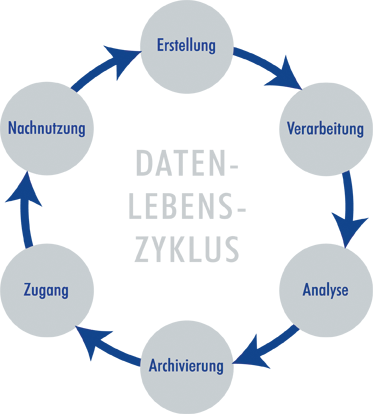
\includegraphics[width=0.51\textwidth]{bilder/Datenlebenszyklus}
  \end{center}
  \caption{Datenlebenszyklus}
\end{wrapfigure}

In der gegenwärtigen Praxis ist der Datenlebenszyklus oft unterbrochen, da nur einige wenige Daten ihren Weg in eine Publikation finden. Die übrigen Daten geraten auf den lokalen Speichermedien der Forscher in Vergessenheit oder werden komplett gelöscht und stehen somit einer Nachnutzung nicht mehr zur Verfügung. Diese Tatsache gilt es für die Zukunft zu verbessern und im Idealfall vollständig zu vermeiden.

Der hier vorgestellte Datenlebenszyklus beruht auf dem des "`UK Data Archive"'\footnote{\url{http://data-archive.ac.uk/create-manage/life-cycle}}. Er beschreibt sehr vereinfacht und idealtypisch die Abfolge der einzelnen Phasen im Zyklus aus einem eher praktischen Umgang mit Forschungsdaten. Es gibt auch andere komplexere Modelle, die einen anderen Blickwinkel beschreiben, wie etwa das "`Curation Lifecycle Model"'\footnote{\url{http://www.dcc.ac.uk/resources/curation-lifecycle-model}}, das verschiedene Tätigkeitsfelder bei der Erhaltung und Pflege der Daten beschreibt, und das "`Data Curation Continuum"'\footnote{\url{http://www.dlib.org/dlib/september07/treloar/09treloar.html}}, das vor allem auf die technischen Bedingungen eingeht und Daten unter dem Gesichtspunkt der Nutzergruppen, von privat bis öffentlich, beschreibt.

In jeder Phase des Datenlebenszyklus gelten unterschiedliche Schwerpunkte mit ihren eigenen Implikationen, die im Folgenden umrissen werden. In dem Kapitel Projektphasen ab Seite \pageref{projektphasen} werden die wichtigsten Aspekte dann ausführlich behandelt.

\subparagraph{Erstellung} Vor der eigentlichen Erstellung von neuen Daten muss schon die Projektplanung erfolgt und die Fragestellung formuliert sein, die maßgeblich bestimmen, wie die gesammelten und erzeugten Daten letztendlich aussehen sollen. Ein Bestandteil der Planung muss auch das Datenmanagement sein, das ab Seite \pageref{datenmanagement} beschrieben wird, um vorab festzulegen, welche Formate und Benennungsregeln verwendet werden sollen, wie die Speicherung und Sicherung der Daten und die Vernetzung von Daten und Projektmitarbeitern untereinander aussehen soll. Bereits vorhandene relevante Daten sollten lokalisiert und berücksichtigt werden. 

Schon während der Erstellung der Forschungsdaten erfolgt idealerweise die Beschreibung der Daten, da diese besonders im Hinblick auf die spätere Nachnutzung für die Verständlichkeit eine elementare Rolle spielt. Beispielsweise müssen die technischen Parameter der verwendeten Aufnahmegeräte so früh wie möglich dokumentiert werden.

\subparagraph{Verarbeitung} Sobald die Daten erhoben wurden, können sie verarbeitet werden. Dazu gehören verschiedene Abläufe, wie etwa Digitalisierung, Übersetzung, Überprüfung, Validierung, Bereinigung und andere Verarbeitungsformen mittels Programmen. Für einige Anwendungen oder im Hinblick auf eine spätere Veröffentlichung, kann eine Anonymisierung notwendig sein. Auch gilt es festzuhalten, wie Ausgangsdaten verändert und bearbeitet wurden. 

Außerdem ist die Beschreibung von Forschungsdaten ein wichtiger Aspekt für die Archivierung, um die Verständlichkeit für die spätere Nachnutzung deutlich zu erhöhen. Während der Verarbeitung von Forschungsdaten spielt die Verwaltung und Speicherung der Daten eine große Rolle, da gewährleistet werden muss, dass mit der richtigen Version gearbeitet wird und notfalls auch Sicherheitskopien zur Verfügung stehen.

\subparagraph{Analyse} Durch die Analyse und Interpretation der Forschungsdaten werden die Forschungsergebnisse gewonnen, die dann in Publikationen veröffentlicht werden. In der Regel sind die den neuen Erkenntnissen zugrunde liegenden Daten aber nur ein kleiner Bestandteil einer solchen Publikation. Jedoch werden alle Daten benötigt, um die Analyseergebnisse vollständig nachvollziehen zu können.

\subparagraph{Archivierung} Die Archivierung von Forschungsdaten beinhaltet die Auswahl und Umwandlung der einzelnen Dateien in geeignete Formate und deren Speicherung auf einem für die Archivierung geeigneten Medium. Die Erstellung und Speicherung von Backups gehört ebenfalls dazu.

Eine wesentliche Rolle bei der Archivierung spielt sowohl die strukturierte als auch die freie Beschreibung der Forschungsdaten, da diese Informationen darüber enthalten, wie und durch wen die Daten gewonnen wurden, welche Geräte dabei Verwendung fanden, wie diese konfiguriert waren und was die Daten bedeuten. 

\subparagraph{Zugang} Da das Ziel einer Datenarchivierung immer die Nachnutzbarkeit von Inhalten ist, sollten archivierte Daten im Rahmen rechtlicher Rahmenbedingungen verbreitet und Dritten ein Zugriff auf diese gewährt werden. Den Zugriff auf die Daten kann man mit verschiedenen Zugriffsrechten steuern, die es beispielsweise nur einer eingeschränkten Gruppe von Nutzern erlauben auf die Daten zuzugreifen. Bevor die Daten zugänglich gemacht werden, sollte man dafür sorgen, dass das Urheberrecht geklärt und gekennzeichnet ist.

Durch die Zugriffsgewährung wird die Sichtbarkeit von eigenen Forschungsleistungen erhöht.

\subparagraph{Nachnutzung} Archivierte Daten, die zugänglich gemacht wurden, können für eigene Forschungsvorhaben kostenlos wiederverwendet und neuen Analysen unterzogen werden. Durch die Nachnutzung wird die Nachprüfbarkeit von Ergebnissen im Sinne der guten wissenschaftlichen Praxis erleichtert.

%Projektphasen
	\chapter{Projektphasen}
	\abschnittsautor{S. Jahn, F. Schäfer, M. Trognitz}
	\label{projektphasen}

Im Umgang mit digitalen Daten gelten für jede Phase eines Forschungsprojektes unterschiedliche Anforderungen und Bedingungen. Da Forschungsdaten einem Lebenszyklus (siehe Seite \pageref{lebenszyklus}) unterliegen, haben Entscheidungen und Arbeitsschritte, die in einer bestimmten Phase getroffen werden, auch Auswirkungen auf die anderen Phase des Datenkreislaufs. Bereits bei Entwurf und Planung eines neuen Forschungsprojektes muss überlegt werden, welche Informationen bereits digital existieren, welche Arten von Dateien neu erzeugt werden müssen, welche Informationstechnologien zum Einsatz kommen sollen und wie das Management der Forschungsdaten gestaltet sein wird. 

Insofern gilt es einige Aspekte so früh wie möglich, häufig noch vor der Erstellung der ersten Datei, zu adressieren:
\begin{itemize}
\item Informationen über existierende Standards und Richtlinien einholen
\item Entscheidungen über die zu verwendenden Dateiformate und Softwareprogramme fällen
\item Verantwortliche für das Datenmanagement bestimmen
\item Kriterien für die laufende Dokumentation entwickeln
\item Konventionen für die Ablage, Benennung und Versionierung von Dateien festlegen
\item Strategien zur Speicherung und Sicherung definieren
\item Geeignete Infrastrukturen für die Archivierung auswählen und kontaktieren
\end{itemize}

Diese und weitere Fragen zur Vorbereitung, Durchführung und Nachbereitung eines Projektes werden im Folgenden anhand eines sogenannten Datenmanagementplans thematisiert. Der Datenmanagementplan bildet einen wichtigen Baustein zur Festlegung der Arbeitsabläufe im Umgang mit Forschungsdaten und für eine Kostenkalkulation.

Je mehr und je früher in den Einzelentscheidungen die Nachnutzung der Daten durch Dritte auch über die Lebensdauer eines Projektes hinaus berücksichtigt wird und die Langzeitarchivierung als kontinuierliche Maßnahme und nicht als letzter Schritt eines bereits abgeschlossenen Projektes begriffen wird, umso leichter gelingt es, einmal erhobene Daten auch für die Zukunft zu erhalten. Die Archivierung der Daten nach Abschluss eines Projektes wird erleichtert, wenn schon während der Durchführung eines Projektes auf die konsequente Erfüllung der im Datenmanagementplan genannten Aufgaben geachtet wird.

Das Finanzierungskonzept eines Forschungsprojektes sollte neben Hard- und Softwareausstattung ausdrücklich angemessene Anteile für Personalkosten und Dienstleistungen berücksichtigen. Im Zweifelsfall ist es ratsam, sich hierbei beraten zu lassen. Ab einer bestimmten Projektgröße bzw. Umfang der zu prozessierenden Daten sollten eine oder mehrere Personalstellen eingeplant werden, die überwiegend oder ausschließlich für IT-Belange zuständig sind. 

Vor oder kurz nach Beginn des Projektes erstellte und kommunizierte Richtlinien, ermöglichen es allen Projektmitarbeitern diese auch einzuhalten. Auf diese Weise wird die Handhabung der Projektdaten erheblich erleichtert, da geregelte Ordnerstrukturen und vorgegebene Namenskonventionen das Auffinden der Daten vereinfachen, die parallele Dokumentation das Verstehen und die Nachnutzung ermöglicht und Sicherungskopien das Risiko eines Datenverlustes reduzieren.

Abweichungen von den hier aufgeführten Empfehlungen sind nicht auszuschließen, doch sollten diese bewusst diskutiert und in Abwägung der jeweiligen Vor- und Nachteile entschieden werden.

\newpage
\section{Datenmanagement}\label{datenmanagement}
\abschnittsautor{M. Trognitz, D. Hagmann, J. Räther, S. Jahn}
Bereits vor Beginn eines Forschungsvorhabens steht die Konzeption und Planung des Projektes. Dazu gehört auch eine Beschreibung über den Umgang mit den resultierenden Forschungsdaten, der sogenannte Datenmanagementplan. Ein vollständiger Datenmanagementplan berücksichtigt alle Phasen des auf Seite \pageref{lebenszyklus} beschriebenen Lebenszyklus von Forschungsdaten. Er dient zunächst als Mittel zur strukturierten Reflexion über datenrelevante Aspekte eines Projektes und beantwortet grundsätzliche Fragen zu Verantwortlichkeiten, Maßnahmen zur Pflege und Verarbeitung der Daten, Standards und bereits vorhandenen Daten. Außerdem bietet er die Grundlage für Arbeitsabläufe (Workflows) im Umgang mit Forschungsdaten und für eine Kostenkalkulation.

Eine vollständige Dokumentation des Datenmanagements in einem Datenmanagementplan spart Zeit und Kosten, wenn beispielsweise Zusammenhänge beim Wechsel von Mitarbeitern hergestellt werden sollen, und beugt einem Datenverlust vor. Da die Nachnutzung von Forschungsdaten zunehmend an Bedeutung gewinnt, setzen Geldgeber oft einen Datenmanagementplan als Teil eines Förderantrags voraus.

Die konsequente Einhaltung aller im Datenmanagementplan gemachten Vorgaben während der gesamten Projektlaufzeit stellt sicher, dass die Daten auch von Dritten interpretiert und nachgenutzt werden können. Wird das Überführen der Daten in ein Archiv schon von Beginn des Projektes an vorbereitet und einkalkuliert ist zum Projektabschluss nur noch ein geringer Aufwand für die Übergabe in ein Archiv erforderlich, weil die Umformatierung, Neustrukturierung oder nachträgliche Dokumentation von Daten wegfällt.

Ein aktives Datenmanagement beugt insbesondere während der Planung und Durchführung eines Projektes späteren Zeit- und Budgetverlusten vor und stellt sicher, dass Daten am Ende in nachhaltigen Formaten, gut dokumentiert und gut strukturiert vorliegen.
% implementing data management measures during the planning and development stages of research will avoid later panic and frustration

\subsection{Übersicht der Aufgaben in den Projektphasen}
Mit Hilfe des zu Beginn eines Projektes erstellten Datenmanagementplans können sämtliche Prozesse während des Projekts strategisch umgesetzt werden, wobei die Umsetzung des Plans als laufender Vorgang zu verstehen ist. Wenn während eines Projektes Änderungen an dem Datenmanagementplan notwendig werden, sollten diese begründet, dokumentiert sowie Arbeitsprozesse und Ergebnisse angepasst werden. Außerdem muss dokumentiert werden wie die Änderungen sich auf bereits bestehende Daten auswirken.

In den unterschiedlichen Phasen des Datenlebenszyklus und des Projektes sind die Aspekte des Datenmanagementplans unterschiedlich stark zu berücksichtigen. Die folgende Tabelle veranschaulicht, wann im Lebenszyklus von Forschungsdaten welchen Aufgaben aus dem Datenmanagement besondere Aufmerksamkeit zuteil werden muss.

In Abhängigkeit der Projektgröße kann der Umfang der Aufgaben des Datenmanagementplanes und der Plan selbst skaliert werden, wobei jedoch Minimalanforderungen einzuhalten sind, um zuallererst die Verfügbarkeit der Daten im laufenden Projekt zu gewährleisten. Um die Planungen zu erleichtern und zu beschleunigen,  sollten bereits vorhandene institutionelle Vorgaben und Infrastrukturen genutzt werden.

\begin{table}[hbt]
\begin{tabular}{r!\tbg c!\tbg c!\tbg c!\tbg c!\tbg c!\tbg c!\tbg c!\tbg}
	\arrayrulecolor{ianusGrau}
 	\multicolumn{1}{r}{} & \multicolumn{1}{c}{\rot{Vorbereitung}} & \multicolumn{1}{c}{\rot{Erstellung}}& \multicolumn{1}{c}{\rot{Verarbeitung}} & \multicolumn{1}{c}{\rot{Analyse}} & \multicolumn{1}{c}{\rot{Archivierung}} & \multicolumn{1}{c}{\rot{Zugang}} & \multicolumn{1}{c}{\rot{Nachnutzung}}\\
	\cline{2-8}
	Rahmendaten\tib{*} & $\tib{\CIRCLE}$ & $\tib{\Circle}$ & $\tib{\Circle}$ & $\tib{\Circle}$ & $\tib{\RIGHTcircle}$ & $\tib{\Circle}$ & $\tib{\Circle}$\\
	\cline{2-8}
	Verantwortlichkeiten\tib{*} & $\tib{\CIRCLE}$ & $\tib{\Circle}$ & $\tib{\Circle}$ & $\tib{\Circle}$ & $\tib{\Circle}$ & $\tib{\Circle}$ & $\tib{\Circle}$\\
	\cline{2-8}
	Rechtliche Aspekte\tib{*} & $\tib{\CIRCLE}$ & $\tib{\Circle}$ & $\tib{\Circle}$ & $\tib{\Circle}$ & $\tib{\CIRCLE}$ & $\tib{\CIRCLE}$ & $\tib{\CIRCLE}$\\
	\cline{2-8}
	Methoden & $\tib{\CIRCLE}$ & $\tib{\CIRCLE}$ & $\tib{\RIGHTcircle}$ & $\tib{\RIGHTcircle}$ & $\tib{\Circle}$ & $\tib{\Circle}$ & $\tib{\Circle}$\\
	\cline{2-8}
	Vorgaben und Standards\tib{*} & $\tib{\CIRCLE}$ & $\tib{\CIRCLE}$ & $\tib{\CIRCLE}$ & $\tib{\Circle}$ & $\tib{\CIRCLE}$ & $\tib{\RIGHTcircle}$ & $\tib{\Circle}$\\
	\cline{2-8}	
	Kosten \& Ressourcen\tib{*} & $\tib{\CIRCLE}$ & $\tib{\CIRCLE}$ & $\tib{\CIRCLE}$ & $\tib{\Circle}$ & $\tib{\RIGHTcircle}$ & $\tib{\Circle}$ & $\tib{\Circle}$\\
	\cline{2-8}
	Externe Partner & $\tib{\CIRCLE}$ & $\tib{\CIRCLE}$ & $\tib{\RIGHTcircle}$ & $\tib{\Circle}$ & $\tib{\Circle}$ & $\tib{\RIGHTcircle}$ & $\tib{\CIRCLE}$\\
	\cline{2-8}
	Hard- und Software\tib{*} & $\tib{\CIRCLE}$ & $\tib{\CIRCLE}$ & $\tib{\RIGHTcircle}$ & $\tib{\RIGHTcircle}$ & $\tib{\Circle}$ & $\tib{\Circle}$ & $\tib{\Circle}$\\
	\cline{2-8}
	Datentypen und Datenformate & $\tib{\RIGHTcircle}$ & $\tib{\CIRCLE}$ & $\tib{\CIRCLE}$ & $\tib{\Circle}$ & $\tib{\CIRCLE}$ & $\tib{\Circle}$ & $\tib{\Circle}$\\
	\cline{2-8}
	Nachnutzung vorhandener Daten\tib{*} & $\tib{\RIGHTcircle}$ & $\tib{\RIGHTcircle}$ & $\tib{\CIRCLE}$ & $\tib{\CIRCLE}$ & $\tib{\Circle}$ & $\tib{\RIGHTcircle}$ & $\tib{\Circle}$\\
	\cline{2-8}
	Datenerzeugung \& -prozessierung\tib{*} & $\tib{\RIGHTcircle}$ & $\tib{\CIRCLE}$ & $\tib{\RIGHTcircle}$ & $\tib{\Circle}$ & $\tib{\RIGHTcircle}$ & $\tib{\RIGHTcircle}$ & $\tib{\Circle}$\\
	\cline{2-8}
	Datenmenge & $\tib{\CIRCLE}$ & $\tib{\CIRCLE}$ & $\tib{\CIRCLE}$ & $\tib{\CIRCLE}$ & $\tib{\RIGHTcircle}$ & $\tib{\Circle}$ & $\tib{\Circle}$\\
	\cline{2-8}
	Dateispeicherung und -sicherung\tib{*} & $\tib{\RIGHTcircle}$ & $\tib{\CIRCLE}$ & $\tib{\CIRCLE}$ & $\tib{\CIRCLE}$ & $\tib{\Circle}$ & $\tib{\Circle}$ & $\tib{\Circle}$\\
	\cline{2-8}
	Dateiverwaltung & $\tib{\RIGHTcircle}$ & $\tib{\CIRCLE}$ & $\tib{\CIRCLE}$ & $\tib{\CIRCLE}$ & $\tib{\RIGHTcircle}$ & $\tib{\Circle}$ & $\tib{\Circle}$\\
	\cline{2-8}
	Dokumentation\tib{*} & $\tib{\RIGHTcircle}$ & $\tib{\CIRCLE}$ & $\tib{\CIRCLE}$ & $\tib{\CIRCLE}$ & $\tib{\CIRCLE}$ & $\tib{\RIGHTcircle}$ & $\tib{\Circle}$\\
	\cline{2-8}
	Qualitätssicherung & $\tib{\RIGHTcircle}$ & $\tib{\CIRCLE}$ & $\tib{\CIRCLE}$ & $\tib{\CIRCLE}$ & $\tib{\CIRCLE}$ & $\tib{\Circle}$ & $\tib{\CIRCLE}$\\
	\cline{2-8}
	Datenaustausch & $\tib{\RIGHTcircle}$ & $\tib{\RIGHTcircle}$ & $\tib{\CIRCLE}$ & $\tib{\CIRCLE}$ & $\tib{\Circle}$ & $\tib{\CIRCLE}$ & $\tib{\Circle}$\\
	\cline{2-8}
	Mittelfristige Datenaufbewahrung & $\tib{\RIGHTcircle}$ & $\tib{\CIRCLE}$ & $\tib{\CIRCLE}$ & $\tib{\CIRCLE}$ & $\tib{\Circle}$ & $\tib{\Circle}$ & $\tib{\Circle}$\\
	\cline{2-8}
	Langfristige Archivierung\tib{*} & $\tib{\RIGHTcircle}$ & $\tib{\RIGHTcircle}$ & $\tib{\RIGHTcircle}$ & $\tib{\RIGHTcircle}$ & $\tib{\CIRCLE}$ & $\tib{\Circle}$ & $\tib{\CIRCLE}$ \\
	\cline{2-8}
	Zugänglichkeit und Nachnutzung & $\tib{\CIRCLE}$ & $\tib{\RIGHTcircle}$ & $\tib{\RIGHTcircle}$ & $\tib{\RIGHTcircle}$ & $\tib{\CIRCLE}$ & $\tib{\CIRCLE}$ & $\tib{\CIRCLE}$\\
	\cline{2-8}
	Projektabschluss & $\tib{\RIGHTcircle}$ & $\tib{\Circle}$ & $\tib{\Circle}$ & $\tib{\Circle}$ & $\tib{\RIGHTcircle}$ & $\tib{\RIGHTcircle}$ & $\tib{\Circle}$\\
	\cline{2-8}
\end{tabular}
\caption{Tabellarische Übersicht über die verschiedenen zu berücksichtigenden Aspekte eines Datenmanagementplans während unterschiedlicher Projektphasen und unter Beachtung des Lebenszyklus von Forschungsdaten. Besonders wichtige, als Minimalanforderung zu betrachtende Aspekte des Datenmanagementplans sind mit einem Stern gekennzeichnet.}
\label{tab:dmp-lebenszyklus}
\end{table}
\begin{table}[h!bt]
\begin{tabular}{cr}
	$\tib{\CIRCLE}$ & Aufgabe ist während der Phase relevant.\\
	$\tib{\RIGHTcircle}$ & Aufgabe ist während der Phase teilweise relevant.\\
	$\tib{\Circle}$ & Aufgabe ist während der Phase nicht relevant.\\
\end{tabular}
\end{table}
\subsection{Datenmanagementplan}
Die einzelnen in einem Datenmanagementplan zu berücksichtigenden Aspekte werden im Folgenden kurz skizziert, wobei diese Liste keinen Anspruch auf Vollständigkeit erhebt, sondern vor allem als Anregung für verschiedene Themenfelder gedacht ist. Zu einigen Aspekten folgen ausführlichere Abschnitte im Anschluss an diese Übersicht. 

Die Aufgaben können grob in drei Phasen gegliedert werden:
\begin{itemize}
    \item Planungsphase (ab Seite \pageref{dmp-planung})
    \item Durchführungsphase (ab Seite \pageref{dmp-durchfuehrung})
    \item Abschlussphase (ab Seite \pageref{dmp-abschluss})
\end{itemize}

\label{dmp-planung}\paragraph{Planungsphase}
In der Planungsphase eines Projektes ist es im Hinblick auf den Datenmanagementplan insbesondere notwendig, die hierfür erforderlichen Ressourcen einzuplanen. Diese stehen in direkter Abhängigkeit von dem allgemeinen Rahmendaten und den anzuwendenden Methoden. Sie umfassen sowohl den technischen, als auch den personellen Aufwand. Neben der allgemeinen Festlegung von Verantwortlichkeiten empfiehlt es sich, für den Datenmanagementplan als ganzes oder spezifischer Teile und Datenarten Datenverantwortliche zu benennen.

\subparagraph{Rahmendaten und administrative Angaben}
\begin{itemize}
    \item Welche allgemeinen Informationen und Rahmenbedingungen des Projektvorhabens kontextualisieren das Vorhaben und die Daten? (z.B. Eckdaten des Projektes wie Titel, Namen der Verantwortlichen, Partner, Methoden und Laufzeit)
    \item Was sind, zusammengefasst, die Ziele und das Vorhaben?
    \item Wer sind die Projektträger und Finanzgeber?
\end{itemize}
Dazu kann auch die Liste für Projektbezogene Metadaten ab Seite \pageref{Metadaten-anwendung} konsultiert werden.

\subparagraph{Verantwortlichkeiten}
\begin{itemize}
    \item Wie werden die Rollen und Zuständigkeiten beim Datenmanagement eingeteilt?
    \item Wer beaufsichtigt die Einhaltung des Datenmanagementplans und der daraus resultierenden Vorgaben?
    \item Wer ist für Hard- und Software zuständig?
    \item Wer kümmert sich um die Sicherung der Daten und Backups?
    \item Wer sind institutionelle Ansprechpartner?
    \item Wer sind sonstige Ansprechpartner?
    \item Wer kümmert sich um die Integrität der Daten?
    \item Wie werden die Verantwortlichkeiten kommuniziert?
    \item Ist für eine Kontinuität bei den Verantwortlichkeiten gesorgt?
    \item Wer bekommt welche Berechtigungen für welche Daten?
    \item Gibt es für bestimmte Datenarten Datenverantwortliche?
\end{itemize}

\subparagraph{Rechtliche Aspekte}
\begin{itemize}
    \item Welche Daten sind urheberrechtlich geschützt?
    \item Welche Daten fallen unter Datenschutz?
    \item Wie werden die Rechte am geistigen Eigentum für die Daten von Beginn an dokumentiert?
    \item Gibt es Anforderungen und Einschränkungen für eine Veröffentlichung der Daten?
    \item Mit welchen Lizenzen sollen die Daten für Dritte zur Verfügung gestellt werden?
\end{itemize}

\subparagraph{Methoden}
\begin{itemize}
    \item Welche Methode oder Grabungsmethode wird angewandt?
    \item Hat die Fundstelle oder das Projektvorhaben Einfluss auf die zu verwendenden Methoden?
    \item Gibt es Richtlinien oder Best-Practices für die eingesetzten Methoden?
    \item Welche Dokumentationsmethoden kommen zum Einsatz?
    \item Beeinflusst die zu verwendende Methode die Datenmenge?
\end{itemize}

\subparagraph{Vorgaben, Richtlinien und Standards}
\begin{itemize}
    \item Gibt es Gesetze, Vorschriften der Institution, der Projektträger, der Geldgeber, der externen Partner, der zuständigen Landesämter, die eingehalten werden müssen?
    \item Kann eine bestehende institutionelle Infrastruktur zur Organisation, Verwaltung und Speicherung der Daten genutzt werden?
    \item Sind externe Standards und Richtlinien für den Umgang mit den Daten bekannt?
    \item Welche Qualitätsvorgaben sind für die verschiedenen Datenarten notwendig?
    \item Müssen eigene Vorgaben definiert werden?
    \item Gibt es Checklisten zur Kontrolle der Einhaltung von Vorgaben?
\end{itemize}

\subparagraph{Kosten und Ressourcen}
\begin{itemize}
    \item Wie hoch werden die anfallenden Kosten für Personal und Technik eingeschätzt?
    \item Berücksichtigt die Kostenkalkulation die Kosten in Abhängigkeit der zu erwartenden Datenmenge?
    \item Fallen weitere Kosten für externe Partner oder Dienstleister an?
    \item Muss mit zusätzlichen Kosten für spezielle Anwendungen, Werkzeuge, Systeme etc. gerechnet werden?
    \item Wie sind die Kosten für die Publikation der Ergebnisse zu erwarten?
    \item Welche Folgekosten sind nach Projektende zu erwarten, beispielsweise für die Archivierung der Forschungsdaten?
    \item Welche weiteren Ressourcen werden benötigt?
    \item Bei reproduzierbaren Daten: Sind die Kosten für eine Aufbewahrung höher als für eine Wiederbeschaffung?
    \item Welche Kosten fallen einmalig an, welche regelmäßig?
    \item Können Kosten durch regelmäßige Aufgaben oder durch eine frühzeitige Berücksichtigung von bestimmten Aufgaben verringert werden? (z.B. Dokumentation, Auswahl für das Archiv)
    \item Wer trägt welche Kosten?
    \item Kann der Standard während der gesamten Laufzeit gehalten werden?
\end{itemize}
Weitere Hinweise zur Planung von Kosten und Ressourcen sind in der Broschüre “Einstieg ins Forschungsdatenmanagement in den Geowissenschaften” des EWIG-Projektes ab Seite 11 zu finden. (http://doi.org/10.2312/lis.14.01)


\label{dmp-durchfuehrung}\paragraph{Durchführungsphase}
Während der Durchführung eines Projektes werden die in der Planungsphase gesammelten und erstellten Vorgaben umgesetzt und deren Einhaltung aktiv kontrolliert, sowie bei Bedarf angepasst. 

Eine zeitnah nach Plan durchgeführte Erstellung, Verarbeitung, Analyse und Dokumentation von Daten und Arbeitsabläufen vermeidet eine lange und kostenintensive Abschlussphase. 

\subparagraph{Externe Partner oder Dienstleister}
\begin{itemize}
    \item Mit welchen externen Partnern soll kooperiert werden?
    \item Welche Dienstleister sollen in Anspruch genommen werden?
    \item Welche Auflagen entstehen dadurch und sind diese mit den eigenen Vorgaben vereinbar?
    \item Wie erfolgt der Datenaustausch?
    \item Bei wem verbleiben die Rechte an den Daten?
    \item Wie werden die verschiedenen Vorgaben und Richtlinien an externe Partner kommuniziert?
\end{itemize}

\subparagraph{Hard- und Software}
\begin{itemize}
    \item Welche Hard- und Software steht zur Verfügung?
    \item Werden spezielle Geräte oder Programme benötigt?
    \item Erfüllen die Systeme die vorgegebenen Auflagen, etablierte Standards und die Anforderungen an ein nachhaltiges Datenmanagement?
    \item Können kostenpflichtige Programme durch frei verfügbare Programme (sogenannte Open-Source-Software) ersetzt werden?
\end{itemize}

\subparagraph{Datentypen und Datenformate}
\begin{itemize}
    \item Welche Daten werden verwendet oder erzeugt? (z.B. Beobachtungs- und Messdaten, prozessierte Daten etc.)
    \item In welchen Formaten werden die Daten erzeugt und in welchen sollen sie gesichert werden?
    \item Welches Dateiformat ist für die Archivierung geeignet?
    \item Gibt es verbreitete Standards, die bei der Wahl des Formats zu beachten sind?
    \item Können offene Formate verwendet werden oder müssen proprietäre verwendet werden und hat das Implikationen für die verwendete Hard- und Software?
\end{itemize}
Weitere Informationen sind in den Kapiteln "`Dateiformate"' ab Seite \pageref{dateiformate} und "`Forschungsmethoden"' ab Seite \pageref{methoden} zu finden.

\subparagraph{Nachnutzung vorhandener Daten}
\begin{itemize}
    \item Gibt es bereits vorhandene Daten, die nachgenutzt werden können?
    \item Wurde nach Datenbeständen im Besitz der eigenen Institution oder von Dritten recherchiert?
    \item Wie sind deren Zugriffsmöglichkeiten und Urheberrechte?
    \item Ist die Qualität der Daten ausreichend? (z.B. geeignete Formate, ausreichend Dokumentation)
    \item Wie wird die Integration zwischen bereits bestehenden und neuen Daten organisiert?
    \item Sind auch analoge Quellen zu berücksichtigen?
\end{itemize}

\subparagraph{Erzeugung und Prozessierung von Daten}
\begin{itemize}
    \item Welche Daten müssen neu erzeugt werden oder können bestehende nachgenutzt werden, um das Projektziel zu erreichen?
    \item Handelt es sich um einmalige Daten oder können sie reproduziert werden?
    \item Welche Rolle spielen die Daten innerhalb des Projektes? (z.B. Dokumentation, Publikation, Nachnutzung etc.)
    \item Gibt es sensible oder besonders schützenswerte Daten?
    \item Kann man Anforderungen potentieller Nachnutzer bei der Datenerzeugung mitberücksichtigen?
\end{itemize}

\subparagraph{Datenmenge}
\begin{itemize}
    \item Wie groß ist die zu erwartende Datenmenge für die Gesamtdauer des Projekts?
    \item Hat das Folgen für die Speicherung und Sicherung der Daten? (z.B. längere Backup-Zeiten)
    \item Ergeben sich daraus besondere Anforderungen an die technische Infrastruktur? (z.B. mehr Speicherplatz)
    \item Fallen verschiedene Bearbeitungsstufen mit verschiedenen Versionen an, die gegebenenfalls ein Versionierungssystem erfordern?
\end{itemize}
Weitere Informationen zur Versionierung sind in dem Abschnitt "`Versionskontrolle"' ab Seite \pageref{versionskontrolle} zu finden.

\subparagraph{Dateispeicherung und -sicherung}
\begin{itemize}
    \item Welche Maßnahmen zur Dateispeicherung und -sicherung sind während des Projekts notwendig?
    \item Auf welcher Hardware sollen die Daten gesichert werden? (z.B. Server oder Festplatten)
    \item Wie oft, womit und durch wen werden Backups durchgeführt?
    \item Wer ist für die Datenspeicherung und -sicherung verantwortlich?
    \item Gibt es ein Disaster Management?
    \item Wurden die Maßnahmen zur Dateiwiederherstellung geprobt?
\end{itemize}
Weitere Informationen sind im Abschnitt "`Dateispeicherung und -sicherung"' ab Seite \pageref{dateispeicherung} zu finden.

\subparagraph{Dateiverwaltung}
\begin{itemize}
    \item Wie sollen Dateien benannt, geordnet und versioniert werden?
    \item Gibt es Benennungsregeln für die Dateien?
    \item Kann auf auf bestehende Vorgaben und Systeme für die Dateiverwaltung zurückgegriffen werden?
    \item Sind Verzeichnisstrukturen logisch nachvollziehbar und selbsterklärend?
    \item Ist die Datenablage dokumentiert?
    \item Wie ist der Umgang mit verschiedenen Dateiversionen geplant?
    \item Ist der Einsatz eines Versionierungssystems notwendig?
    \item Werden Daten, die für eine künftige Nachnutzung geeignet sind oder archiviert werden sollen, gesondert verwaltet?
\end{itemize}
Weitere Informationen sind im Abschnitt "`Dateiverwaltung"' ab Seite \pageref{dateiverwaltung} zu finden.

\subparagraph{Dokumentation}
\begin{itemize}
    \item Wie sollen die Daten beschrieben werden, damit sie kurz- und langfristig lesbar und verständlich sind?
    \item Welche Informationen sind zur Dokumentation der Forschungsdaten notwendig?
    \item Zu welchem Zeitpunkt muss die Dokumentation geschehen?
    \item Gibt es Vorgaben oder Standards dafür?
    \item Werden Veränderungen und Aktualisierungen der Daten dokumentiert?
    \item Wie sollen Metadaten abgelegt und gespeichert werden?
    \item Werden Anpassungen an der Projektstruktur und dem Datenmanagementplan dokumentiert?
    \item Werden Ausnahmen dokumentiert?
    \item Gibt es Werkzeuge, die den Dokumentationsprozess unterstützen?
\end{itemize}
Weitere Informationen sind im Abschnitt "`Dokumentation"' ab Seite \pageref{Metadaten-allgemein} zu finden.

\subparagraph{Qualitätssicherung}
\begin{itemize}
    \item Welche Kriterien sind hinsichtlich vorhandener Standards zur Qualitätssicherung zu beachten?
    \item Wie werden Vorgaben zu Formaten und zur Datenbearbeitung eingehalten?
    \item Sind die Daten genau, konsistent und authentisch?
    \item Sind die Daten vollständig?
    \item Wie steht es um die Integrität der Daten?
    \item Sind die Daten verständlich Dokumentiert und geht aus der Dokumentation hervor: \emph{Wer} hat \emph{wann}, zu welchem \emph{Zweck}, \emph{was} und \emph{womit} gemacht?
    \item Wird eine Qualitätskontrolle durchgeführt?
    \item Gibt es Checklisten zur unterstützung der Qualitätskontrolle?
    \item Welche Maßnahmen gegen ein versehentliches Löschen oder eine Manipulation der Daten werden getroffen?
\end{itemize}

\subparagraph{Datenaustausch}
\begin{itemize}
    \item Wie ist der Datenaustausch zwischen den Projektbeteiligten geplant?
    \item Welche technische Infrastruktur ist für den Datenaustausch erforderlich?
    \item Sind gesetzliche Vorgaben oder andere Einschränkungen zu beachten?
    \item Wie soll auf die Daten zugegriffen werden?
    \item Welche Nutzungsrechte liegen für die Daten vor?
\end{itemize}


\label{dmp-abschluss}\paragraph{Abschlussphase}
In der das Projekt abschließenden Phase müssen besonders Entscheidungen sowohl zur mittelfristigen Datenaufbewahrung, als auch zur langfristigen Archivierung der im Projekt generierten Daten und Ergebnisse getroffen werden. Neben der Klärung der organisatorischen und rechtlichen Rahmenbedingungen muss hierbei spezielles Augenmerk auf die Regelung der Zugänglichkeit zu den langzeitarchivierten Daten und der Nachnutzung gelegt werden. So wird sichergestellt, dass über den Projektabschluss hinaus die Daten langfristig zur Verfügung stehen. 

\subparagraph{Mittelfristige Datenaufbewahrung}
\begin{itemize}
    \item Welche Gründe gibt es für eine Aufbewahrung der Daten?
    \item Liegen Vorgaben zur Aufbewahrungsdauer der Daten vor?
    \item Liegen Vorgaben zu Aufbewahrungsorten der Daten vor?
    \item Welche Daten sollen oder müssen aufbewahrt werden, welche Daten sollen oder können gelöscht werden?
    \item Sind sie selbst Hersteller der Daten?
    \item Ist die Aufbewahrung von Fremddaten zwingend notwendig?
    \item Wie lange sollen die Daten aufbewahrt werden?
    \item Wie und wo sollen die Daten aufbewahrt werden?
    \item Wer ist für die Aufbewahrung der Daten verantwortlich?
    \item Sind Kosten zu erwarten?
\end{itemize}

\subparagraph{Vorbereitung für die langfristige Archivierung}
\begin{itemize}
    \item Welche Daten sollen archiviert werden?
    \item Liegen Kriterien für die Auswahl der Daten vor?
    \item Gibt es eine passende Archivlösung?
    \item Wurde bereits Kontakt mit dem Archiv aufgenommen?
    \item Welche Besonderheiten gilt es zu beachten? (z.B. eine gesonderte Aufbereitung der Daten)
    \item Wann und durch wen werden die Daten übergeben?
\end{itemize}

\subparagraph{Zugänglichkeit und Nachnutzung}
\begin{itemize}
    \item Wie sollen die Daten zugänglich sein?
    \item Welche Zusatzinformationen sind für das Verständnis der Daten notwendig?
    \item Wer darf die Daten nutzen, welche Lizenzen sollen verwendet werden?
    \item Gibt es Einschränkungen für den Zugriff auf und die Nutzung der Daten?
    \item Auf welche Weise sollen die Daten zur Verfügung gestellt werden?
\end{itemize}

\subparagraph{Projektabschluss}
\begin{itemize}
    \item Liegt die Dokumentation vollständig und den Vorgaben entsprechend vor?
    \item Ist eine gesonderte abschließende Dokumentation erforderlich?
    \item Ist der Datenmanagementplan in die Dokumentation integriert?
    \item Ist die Nachnutzbarkeit der Forschungsdaten auch nach Projektende gewährleistet?
    \item Wie ist die mittelfristige Aufbewahrung der Daten geregelt?
    \item Wie ist die langfristige Archivierung der Daten geregelt?
    \item Wie ist die Zugänglichkeit der Daten geregelt?
\end{itemize}

%XXX Grafik zur Visualisierung vom DMP: Mit Waben oder Puzzleteilen

\subsection{Weiterführende Informationen}
\paragraph{Quellen}
\begin{flushleft}
Archaeology Data Service, Planning for the Creation of Digital Data \urllist{http://guides.archaeologydataservice.ac.uk/g2gp/CreateData_1-0}
Archaeology Data Service, Data Management and Sharing Plans \urllist{http://archaeologydataservice.ac.uk/advice/DataManagementPlans}
Archaeology Data Service, DataTrain. Open Access Post-Graduate Teaching Materials in Managing Research Data in Archaeology \urllist{http://archaeologydataservice.ac.uk/learning/DataTrain}
S. Büttner --  H.-C. Hobohm -- L. Müller (Hrsg.) Handbuch Forschungsdatenmanagement (Bad Honnef 2011)\abstand
DCC (Hrsg.) Data Management Plans \urllist{http://www.dcc.ac.uk/resources/data-management-plans}
Helmholtz-Zentrum Potsdam - Deutsches GeoForschungsZentrum GFZ -- Bibliothek und Informationsdienste -- Institut für Meteorologie der FU Berlin -- Konrad-Zuse-Zentrum für Informationstechnik Berlin (Hrsg.) Einstieg ins Forschungsdatenmanagement in den Geowissenschaften (2014), DOI: 10.2312/lis.14.01 \urllist{http://doi.org/10.2312/lis.14.01}
HU Berlin (Hrsg.)  Datenmanagementplan. Anleitung zur Erstellung eines Datenmanagementplans (DMP) \urllist{https://www.cms.hu-berlin.de/de/dl/dataman/arbeiten/dmp_erstellen}
U. Jakobsson, Data Management Planning. What it is and how to do it (2013) \urllist{http://www.ariadne-infrastructure.eu/fre/Events/ARIADNE-Workshop-EAA-2013/Agenda-Presentations/DataManagementPlanning_SND_Ujakobsson_04092013}
H. Neuroth -- A. Oßwald -- R. Scheffel -- S. Strathmann -- M. Jehn (Hrsg.) nestor Handbuch. Eine kleine Enzyklopädie der digitalen Langzeitarchivierung. Version 2.0 (2009) Kap.3:15 \abstand
K. Perrin -- D. H. Brown -- G. Lange -- D. Bibby -- A. Carlsson -- A. Degraeve -- M. Kuna -- Y. Larsson -- S. U. Pálsdóttir -- B. Stoll-Tucker -- C. Dunning -- A. Rogalla von Bieberstein, A Standard and Guide to Best Practice for Archaeological Archiving in Europe, EAC Guidelines 1 (2013) \urllist{http://archaeologydataservice.ac.uk/arches/Wiki.jsp?page=The\%20Standard\%20and\%20Guide\%20to\%20Best\%20Practice\%20in\%20Archaeological\%20Archiving\%20in\%20Europe}
UK Data Archive (Hrsg.) Create \& Manage Data. Planning for Sharing \urllist{http://data-archive.ac.uk/create-manage/planning-for-sharing}
Uni Marburg (Hrsg.) Projekt "Kompetenzzentrum Forschungsdatenmanagement und -archivierung" \urllist{https://www.uni-marburg.de/projekte/forschungsdaten}
V. van den Eynden -- L. Corti -- M. Woollard -- L. Bishop -- L. Horton, Managing and Sharing Data. Best Practice for Researchers (Essex 2011) \urllist{http://ukdataservice.ac.uk/manage-data/handbook.aspx}
WissGrid (Hrsg.) Leitfaden Forschungsdaten-Management (2011) \urllist{http://www.wissgrid.de/publikationen/deliverables/wp3/WissGrid-oeffentlicher-Entwurf-Leitfaden-Forschungsdaten-Management.pdf}

\quelltyp{Beispiele für Datenmanagementpläne}
DataONE (Hrsg.) Data Management Planning \urllist{https://www.dataone.org/data-management-planning}
DCC (Hrsg.) Data plan guidance and examples \urllist{http://www.dcc.ac.uk/resources/data-management-plans/guidance-examples}
MITLibraries (Hrsg.) Write a Data Management Plan \urllist{http://libraries.mit.edu/data-management/plan/write/\#Resources}

\quelltyp{Checklisten und Tools für Datenmanagementpläne}
DCC (Hrsg.) Checklist for a Data Management Plan (2014) \urllist{http://www.dcc.ac.uk/webfm_send/1279}
DCC (Hrsg.) DMPOnline \urllist{https://dmponline.dcc.ac.uk/}
J. Richards, Online Resources for Data Management Planning (2013) \urllist{http://www.ariadne-infrastructure.eu/fre/Events/ARIADNE-Workshop-EAA-2013/Agenda-Presentations/DataManagementPlanning_Online_Resources_ADS_JRichards_04092013}
RDMO (Hrsg.) Research Data Management Organiser \urllist{http://rdmorganiser.github.io/software/}
WissGrid (Hrsg.) Checkliste zum Forschungsdaten-Management (2011) \urllist{http://www.wissgrid.de/publikationen/deliverables/wp3/WissGrid-oeffentlicher-Entwurf-Checkliste-Forschungsdaten-Management.pdf}
\end{flushleft}

\newpage
\section{Dokumentation}\label{Metadaten-allgemein}
\abschnittsautor{D. Bibby, P. Gerth, M. Heinrich, S. Jahn, B. Ludwig, A. Posluschny, E. Siegloff, A. Sieverling, M. Trognitz}
\hyphenation{
}

Das wichtigste Kriterium für die Archivierung und Nachnutzbarkeit von Daten ist neben technischen Aspekten, wie die Wahl eines geeigneten Langzeitformates, eine vollständige Dokumentation . Viele Dokumente und Dateien sind nicht aus sich selbst heraus verständlich. Sie stehen immer in einem gewissen Forschungs- oder Projektkontext, der für die Nachnutzung dokumentiert werden muss. Damit Forschungsdaten von Dritten gefunden und sinnvoll verwertet werden können, müssen sie durch zusätzliche Informationen ergänzt und strukturiert beschrieben werden. Wenn Daten ausreichend fachlich wie technisch beschrieben werden, können sie durch andere Personen wissenschaftlich nachgenutzt werden und besitzen somit einen Wert für die Zukunft. Nur dann lohnt sich auch der Aufwand einer analogen oder digitalen Langzeitarchivierung.

Die Dokumentation eines Projektes und der erzeugten Daten sollte als ein wichtiger, kontinuierlicher Prozess verstanden werden, der von Anfang an berücksichtigt und während des gesamten Lebenszyklus von Daten umgesetzt wird -- und nicht erst nach Abschluss von Arbeiten oder bei der Übergabe von Beständen an ein Archiv. Insofern bedarf es innerhalb von größeren Projekten eines Verantwortlichen oder einer Organisationsform aller Beteiligten, welche die Struktur und Pflege der Dokumentation konzeptionell und koordinierend begleitet. Gemeinsam muss definiert werden, welcher Gegenstand dokumentiert wird, in welchem Umfang und mit welcher Gliederung, welche Form geeignet ist (z. B. Wiki versus PDF), wie die Aktualität der Inhalte erhalten wird, wie Nutzer über Änderungen informiert werden usw. Fehlende Strategien für den Aufbau und die Pflege einer Dokumentation führen häufig zu Unübersichtlichkeit und dadurch zu einer Konfusion der beteiligten Akteure. Von umfassenden, detaillierten und strukturierten Angaben zu  digitalen Daten profitieren nicht nur die Archive und zukünftige Generationen von Forschern, sondern auch die Wissenschaftler selbst während der Durchführung eines Projektes -- genauso wie es auch bei einer guten analogen Dokumentenablage der Fall ist.

Welche Informationen sind für eine Dokumentation erforderlich? Wichtig sind alle Angaben, die den Entstehungsprozess und -kontext sowie die Konventionen von Inhalten und Daten beschreiben oder zumindest skizzieren. Dabei kann die Dokumentation als "`Beipackzettel"' verstanden werden, der anderen Personen das Auffinden der Daten, das Verstehen der Inhalte, eine sinnvolle Wiederverwendung der Daten für weitere Forschungen ermöglicht und die Vergleichbarkeit von Daten erhöht. So ist es beispielsweise üblich, bei Fotografien das Aufnahmedatum, eine Kurzbeschreibung des abgelichteten Gegenstandes und den Fotografen anzugeben, Zeichnungen mit einem Maßstab, der geografischen Ausrichtung, dem Zeichner und einem Kurztext zu beschriften oder bei Texten einen Autor, einen Titel und ein Datum zu nennen.

Insbesondere bei digitalen Daten sind zusätzliche, spezialisierte Informationen erforderlich, die über die rein deskriptiven Angaben zu den Inhalten und zum Forschungsinteresse hinausgehen und nicht nur die primären Fragen zu \emph{"`Wer, Wie, Was, Wo, Wann und Warum?"'} beantworten. So sind technische und administrative Angaben über die Vorgehensweise der Datenerhebung und die eingesetzten Programme, mit denen die Daten erzeugt oder digitalisiert wurden, für ein späteres Auslesen, Auswerten und Interpretieren unverzichtbar. Auch wie die Daten strukturiert wurden und in welcher Beziehung Dateien zueinander stehen, muss in der Regel explizit erklärt werden. Angaben zu Qualitätssicherungsverfahren,  Änderungshistorie und Versionierung von Daten erlauben es, das empirische Vorgehen im Forschungsprozess nachzuprüfen. Zudem ist es wichtig zu erklären, wie Dritte zukünftig auf die Daten zugreifen  oder sie nutzen dürfen.

Damit unbeteiligte Personen den größeren Zusammenhang einer einzelnen Information oder eines Datenbestandes verstehen und nachvollziehen können, sollte jede Dokumentation eines Projektes mindestens folgende Punkte enthalten:
\begin{itemize}
	\item Angaben zur Fragestellung und zum Untersuchungsgegenstand
	\item Angaben zu den Projektverantwortlichen für Nachfragen
	\item Zusammenfassung der wissenschaftlichen Ergebnisse
	\item Beschreibung von Arbeitsabläufen und Methoden, vor allem bezüglich der Datenerhebung, -verarbeitung und Qualitätssicherung
	\item Auflistung der erzeugten unterschiedlichen Dokumentarten (z. B. Tagebücher, Berichte, Listen, Fotos etc.)
	\item Beschreibung von verwendeten Handbüchern, Standards, projektspezifischen Konventionen, Thesauri, Nummernsystemen etc.
	\item Auflistung der eingesetzten technischen Geräte und Programme
	\item Relevante Publikationen und wichtige Sekundärliteratur
	\item Wichtige Korrespondenzen, Verträge, Anträge etc. (ggf. in anonymisierter Form) 
	\item Bestimmungen zur weiteren freien oder eingeschränkten Verwendung von Daten
\end{itemize}

In dem Abschnitt Speicherung von Metadaten ab Seite \pageref{metadatenSpeicherung} sind weitere allgemeine Angaben zu finden. In dem Kapitel Dateiformate ab Seite \pageref{dateiformate} werden außerdem weitere notwendige Angaben abhängig vom Dateityp aufgelistet. Auch für die Anwendung von bestimmten Methoden werden gesonderte Dokumentationsangaben erforderlich, die in dem Kapitel Forschungsmethoden ab Seite \pageref{methoden} zu finden sind.


%##################################################################################

\subsection{Dokumentation mit Metadaten}
Ein spezifischer Bestandteil einer jeden Dokumentation sind Metadaten. Während die Dokumentation die Summe aller Angaben zu einem Projekt und der zugehörigen Daten umfasst und sie in Form, Inhalt, Länge und Struktur je nach fachlichen Gepflogenheiten völlig frei formuliert sein kann, sind Metadaten nach festen formalen Kriterien strukturiert (z. B. als Formulare oder Eingabemasken) und beschreiben die Eigenschaften von anderen Daten, ohne diese selbst zu enthalten.

Metadaten machen die fachlich oder organisatorisch notwendigen Kontextinformationen explizit und dienen zur Auffindung von relevanten Informationen, deren Identifikation, deren Auswahl und Verwaltung. Beispielsweise sind Fotos nur anhand der mit ihnen assoziierten beschreibenden Metadaten effizient durchsuch- und auffindbar oder Karten nur dank einer Maßstabsangabe und einer aussagekräftigen Legende wissenschaftlich nutzbar. Die National Information Standards Organization (NISO) definiert Metadaten als Werkzeuge, um Forschungsdaten nachhaltig zu organisieren, zu erschließen, zu verstehen und zu benutzen. Werden Metadaten standardisiert gespeichert, können sie auch maschinell verarbeitet werden.

Da Metadaten immer von unterschiedlichen Informationsbedürfnissen und Anwendungskontexten abhängig sind, lassen sie sich unter verschiedenen Blickwinkeln betrachten. Egal ob sie ein Forschungsvorhaben in seiner Gesamtheit oder den Inhalt eines einzelnen Dokuments beschreiben, können sie sich auf folgende Aspekte beziehen:
\begin{itemize}
	\item Deskriptive Angaben, die ein Projekt, ein Objekt oder eine Methode fachlich und inhaltlich näher beschreiben (z. B. Kurzbeschreibung eines Fotos, Laufzeit eines Forschungsvorhabens, Autor eines Textes)
	\item Strukturelle Angaben, welche die physischen oder logischen Beziehungen zwischen komplexen Objekten beschreiben (z. B. referenzierte Dateien in Zeichnungen, die Reihenfolge von Fotos oder zusammengehörige Dateien)
	\item Administrativ-rechtliche Angaben, die Rechteinhaber, Lizenzbedingungen und Zugangsregeln benennen und für die Verwaltung relevant sind (z. B. Fristen für die Veröffentlichung von Ergebnissen)
	\item Administrativ-erhaltungsbezogene Angaben, welche die Geschichte eines digitalen Objektes, also die  vorhergehenden und gegenwärtigen Zustände, nachvollziehen lassen und Erhaltungsmaßnahmen beschreiben (z. B. Angabe zur Herkunft einer Karte, Konvertierungsmaßnahmen)
	\item Technische Angaben, die Informationen zu Software und Hardware liefern (z. B. das Dateiformat eines Bildes, die Zeichenkodierung eines Textes oder technische Parameter eines Messgerätes). Sie werden benötigt, um Daten in veralteten Dateiformaten in neuere umwandeln oder um die ursprüngliche Programmumgebung mittels aktueller Technik nachbauen zu können.
\end{itemize}

Ein anderes Unterscheidungskriterium von Metadaten ist der Umfang der Daten, die sie beschreiben. Sie können sich beziehen auf:
\begin{itemize}
	\item Eine größere zusammenhängende Datensammlung (z. B. der gesamte Datenbestand eines Projektes)
	\item Eine einzelne Datei
	\item Eine einzelne Information innerhalb eines Systems (z. B. ein Datensatz in einer Datenbank)
\end{itemize}

Weiterhin können Metadaten auch angewandte Prozesse und Methoden beschreiben, um den Entstehungsprozess von Dateien und Dateikonvoluten verständlicher zu machen und Hinweise für den weiteren Umgang mit den Daten zu liefern. Im Abschnitt Metadaten in der Anwendung ab Seite \pageref{Metadaten-anwendung} werden daher Metadaten in drei Kategorien unterschieden:
\begin{itemize}
	\item Projektbezogene Metadaten, die den gesamten Datenbestand eines Projektes dokumentieren
	\item Dateibezogene Metadaten, die einzelne Dateien dokumentieren
	\item Methodenbezogene Metadaten, die angewandte Prozesse und Methoden dokumentieren
\end{itemize}

Außerdem kann bei Metadaten unterschieden werden zwischen solchen, die eine manuelle Eingabe erfordern, und solchen, die durch Systeme und Programme automatisch erzeugt werden können. Erstere können beispielsweise eine Kurzbeschreibung oder Schlagworte sein. Letztere sind Angaben wie Erstellungsdatum, Dateiname oder Einstellungen der Digitalkamera.

Während für ein laufendes Projekt nur ein Ausschnitt dieser Metadaten eine praktische Relevanz besitzt, sind für die digitale Langzeitarchivierung von Daten alle Aspekte wichtig. Einige der Metadaten können ausschließlich von beteiligten Personen frühzeitig während des Prozesses der Datenerzeugung erfasst werden, da nur sie den Inhalt, den Charakter, die Struktur, den Kontext und die Quellen der Daten kennen. Andere Metadaten dagegen lassen sich auch zu einem späteren Zeitpunkt bei der Archivierung und Veröffentlichung der Daten generieren.


%##################################################################################

\subsection{Strukturierung von Metadaten}
Die Struktur und der Umfang von Metadaten sind wesentliche Faktoren, um diese sinnvoll nutzen zu können. Die Art und Weise, wie die verschiedenen Informationen erfasst und organisiert werden, spielen dabei eine zentrale Rolle, ob sie von einer unbeteiligten dritten Person richtig verstanden werden und ob die Angaben automatisiert verarbeitet werden können. 

Um die Struktur und den Umfang von Metadaten verbindlich zu beschreiben und vorzugeben, werden Metadatenschemata verwendet. Ein Metadatenschema gibt den Inhalt und die Gliederung von Metadaten vor, also die zu verwendenden Metadaten-Kategorien. Beispielsweise kann eine Publikation mit den Attributen Autor -- Jahr -- Titel -- Reihe -- Verlag -- Erscheinungsort und Schlagworte beschrieben werden, die dann mit den entsprechenden Informationen gefüllt werden. Diese Minimalbeschreibung kann je nach Anforderungen erweitert werden, etwa um die Elemente Sprache -- Seitenzahl -- Abbildungszahl -- Auflage und ISBN-Nummer.

In einem Metadatenschema wird zudem für einzelne Informationen die Genauigkeit (die Granularität) der erwarteten Information festgelegt, also ob beispielsweise für das Attribut "`Autor"' eine freie Texteingabe ausreichend ist oder ob eine Aufteilung in die Teilattribute Anrede -- Titel -- Vorname(n) und Nachname sowie eine Referenz zu einer Personennormdatei erforderlich ist.

Für den Austausch von Metadaten zwischen verschiedenen technischen Systemen besitzen die zugrunde liegenden Schemata eine zentrale Bedeutung. Sollen Informationen aus unterschiedlichen Quellen miteinander in Beziehung gesetzt werden, so dass sie gemeinsam ausgewertet werden können, müssen die jeweils eingetragenen Werte auf der Ebene ihrer semantischen Bedeutung miteinander verknüpft und abgeglichen werden. Das heißt, dass neben dem eigentlichen Wert (z. B. die Zeichenkette "`Pompeji"') auch das Attribut angegeben werden muss, also die Eigenschaft, die durch den Wert beschrieben wird (z. B. "`Fundort"', "`Aufbewahrungsort"' oder "`Publikationsort"'). 

Für viele Bereiche, wie etwa Medienarchive, Bibliotheken oder Museen, gibt es langjährige Erfahrungen im Umgang mit Metadaten und es wurden spezifische Metadatenschemata entwickelt. Zu Beginn eines Projektes sollte geprüft werden, ob relevante Metadatenschemata bereits existieren oder sogar vorgegeben werden und bei der Erzeugung von eigenen Metadaten berücksichtigt werden sollten. Je internationaler und standardisierter ein verwendetes Schema ist, desto eher ist die Austauschbarkeit von Metadaten mit anderen Systemen gewährleistet. Sofern sich unterschiedliche Metadaten auf ein gemeinsames Metadatenschema abbilden (\emph{mappen}) lassen, können sie in ein drittes System importiert und dort gemeinsam geöffnet werden.

\begin{wrapfigure}{r}{0.5\textwidth}
  \begin{center}
    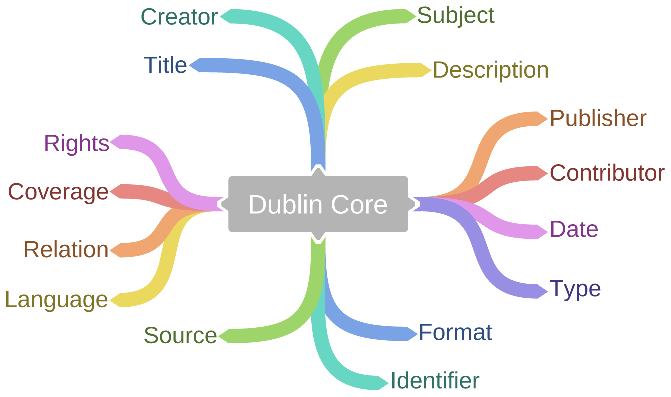
\includegraphics[width=0.5\textwidth]{bilder/doku_dublinCore}
  \end{center}
  \caption{Die 15 Kernfelder von Dublin Core Version 1.1. (Grafik erstellt mit coggle.it.)}
  \label{doku_dublinCore}
\end{wrapfigure}
Für deskriptive Metadaten ist das unter ISO 15836 zertifizierte Metadatenschema \emph{Dublin Core} (in Abbildung \ref{doku_dublinCore}) am weitesten verbreitet. Es verfügt in der Version 1.1 über folgende 15 Kernfelder: \emph{Title} (Titel) -- \emph{Creator} (Ersteller) -- \emph{Subject} (Thema) -- \emph{Description} (Beschreibung) -- \emph{Publisher} (Verleger) -- \emph{Contributor} (Mitwirkender) -- \emph{Date} (Datum) -- \emph{Type} (Typ) -- \emph{Format} (Format) -- \emph{Identifier} (Identifikator) -- \emph{Source} (Quelle) -- \emph{Language} (Sprache) -- \emph{Relation} (Beziehung) -- \emph{Coverage} (Umfang) -- \emph{Rights} (Rechte).

Im Laufe der Jahre wurde dieses grundlegende Set noch erweitert. Das aktuelle Set, "`\emph{The Dublin Core Metadata Initiative (DCMI) Metadata Terms}"', und die Beschreibung der einzelnen Attribute kann \href{http://dublincore.org/documents/dcmi-terms/}{online}\footnote{\href{http://dublincore.org/documents/dcmi-terms/}{http://dublincore.org/documents/dcmi-terms/}} abgerufen werden.

Eine besondere Relevanz im archäologischen und altertumswissenschaftlichen Kontext haben folgende Standards erlangt:
\begin{itemize}
	\item Online AccesS to the Index of archaeological investigationS (OASIS), veröffentlicht von English Heritage. Es wurde für den Nachweis von archäologischen Projekten und Maßnahmen in Großbritannien entwickelt. Das Schema liegt aktuell in Version 1.3 vor. Neben den in der Abbildung \ref{abb:doku_oasisProject} dargestellten fünf Themenbereichen können auch weitere spezielle Angaben wie etwa zu Arealen, Geophysik, Geologie und Artefakten gemacht werden.
	\begin{figure}[h!bt]
		\begin{center}
			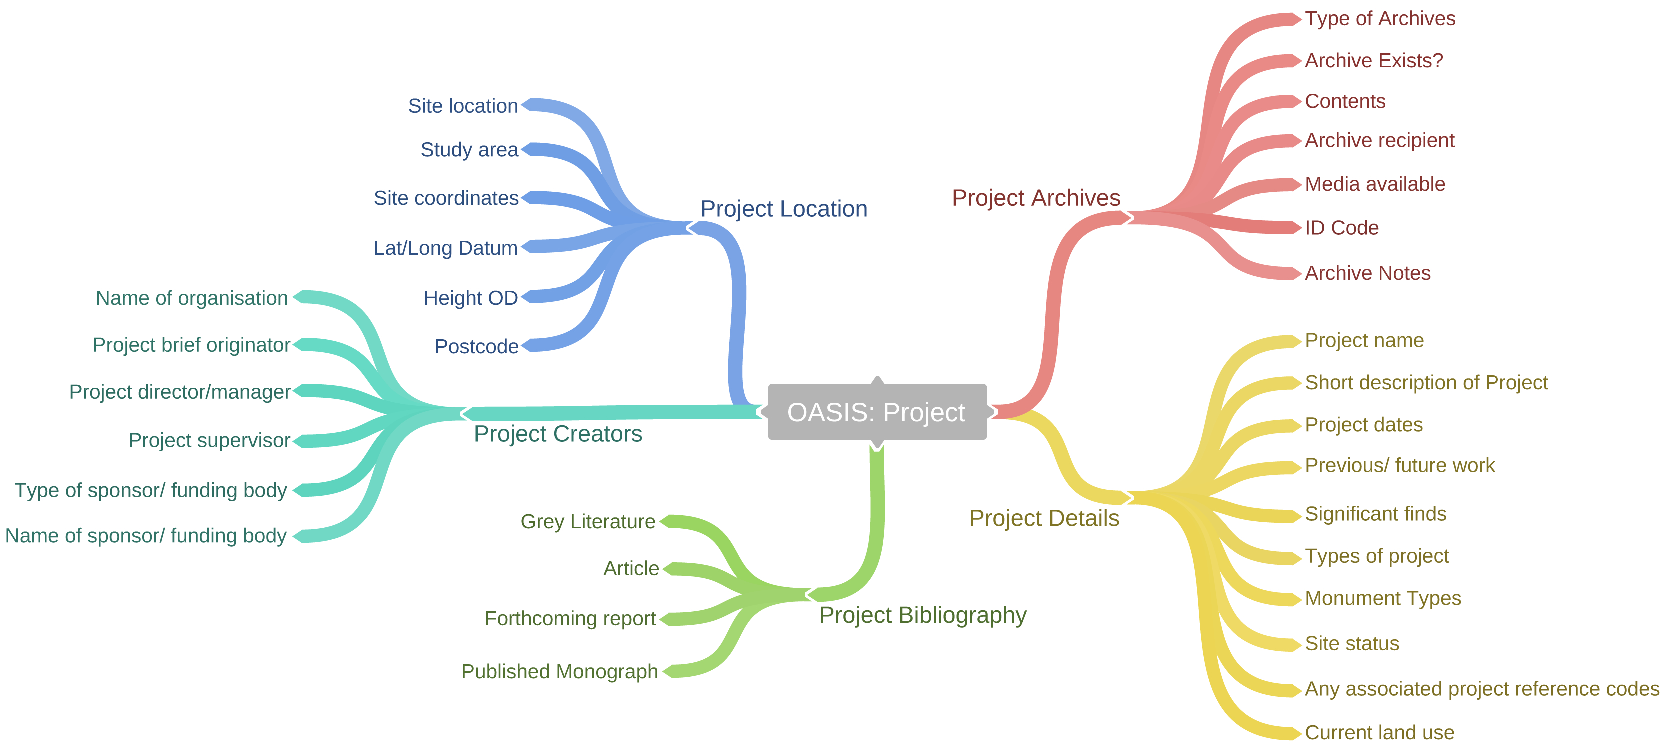
\includegraphics[width=\textwidth]{bilder/doku_oasisProject}
		\end{center}
		\caption{OASIS in Version 1.3. Neben den abgebildeten Themenbereichen sind auch Attribute für weitere spezialisiertere Informationen vorgesehen. (Grafik erstellt mit coggle.it.)}
		\label{abb:doku_oasisProject}
\end{figure}
	\item Archäologischer DateneXport-Standard (ADeX), wurde von der "`Kommission Archäologie und Informationssyteme"' beim Verband der Landesarchäologen entwickelt. Der Standard wurde für den Austausch archäologischer Fachdaten zwischen Landesämtern und anderen Institutionen erarbeitet. Die aktuelle in Abbildung \ref{abb:doku_ADeX} dargestellte Version ist 2.0, die auch den Austausch von komplexen Geometrien mittels externer Geometriedaten (SHP oder MIF) ermöglicht. ADeX ist bewusst als einfaches Austauschformat mit den Teilen "`Generelles"', "`Georeferenz"' und  "`Typ und Zeit"' unter Berücksichtigung internationaler Standards, wie etwa CIDOC-CRM, gestaltet. Dies gewährleistet eine hohe Austauschbarkeit.
	\begin{figure}[h!bt]
		\begin{center}
			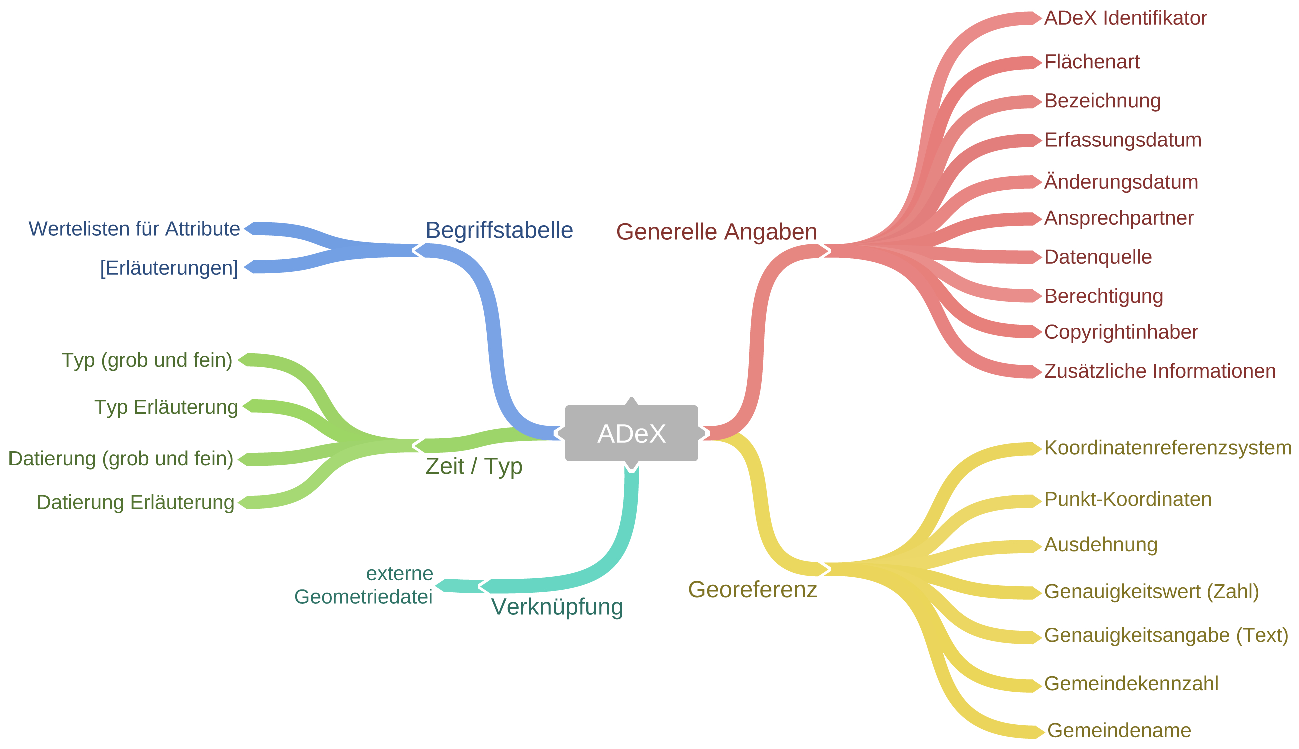
\includegraphics[width=\textwidth]{bilder/doku_ADeX}
		\end{center}
		\caption{ADeX in Version 2.0, das für eine hohe Kompatibilität auf detailliete Informationen verzichtet. (Grafik erstellt mit coggle.it.)}
		\label{abb:doku_ADeX}
\end{figure}
	\item Connecting Archaeology and Architecture in Europeana (CARARE) in Version 2.0. Es wurde als archäologiespezifisches Datenmodell unter Berücksichtigung verschiedener europäischer Standards von Europeana und dem Project 3D-ICONS entwickelt. Die Abbildung \ref{abb:doku_CARARE} verdeutlicht, dass in dem Schema Informationen zur Sammlung (\emph{Collection information}), zum physischen Objekt (\emph{Heritage asset}), zur digitalen Ressource (\emph{Digital resource}) und zur Aktivität (\emph{Activity}) definiert werden.
	\begin{figure}[h!tb]
		\begin{center}
			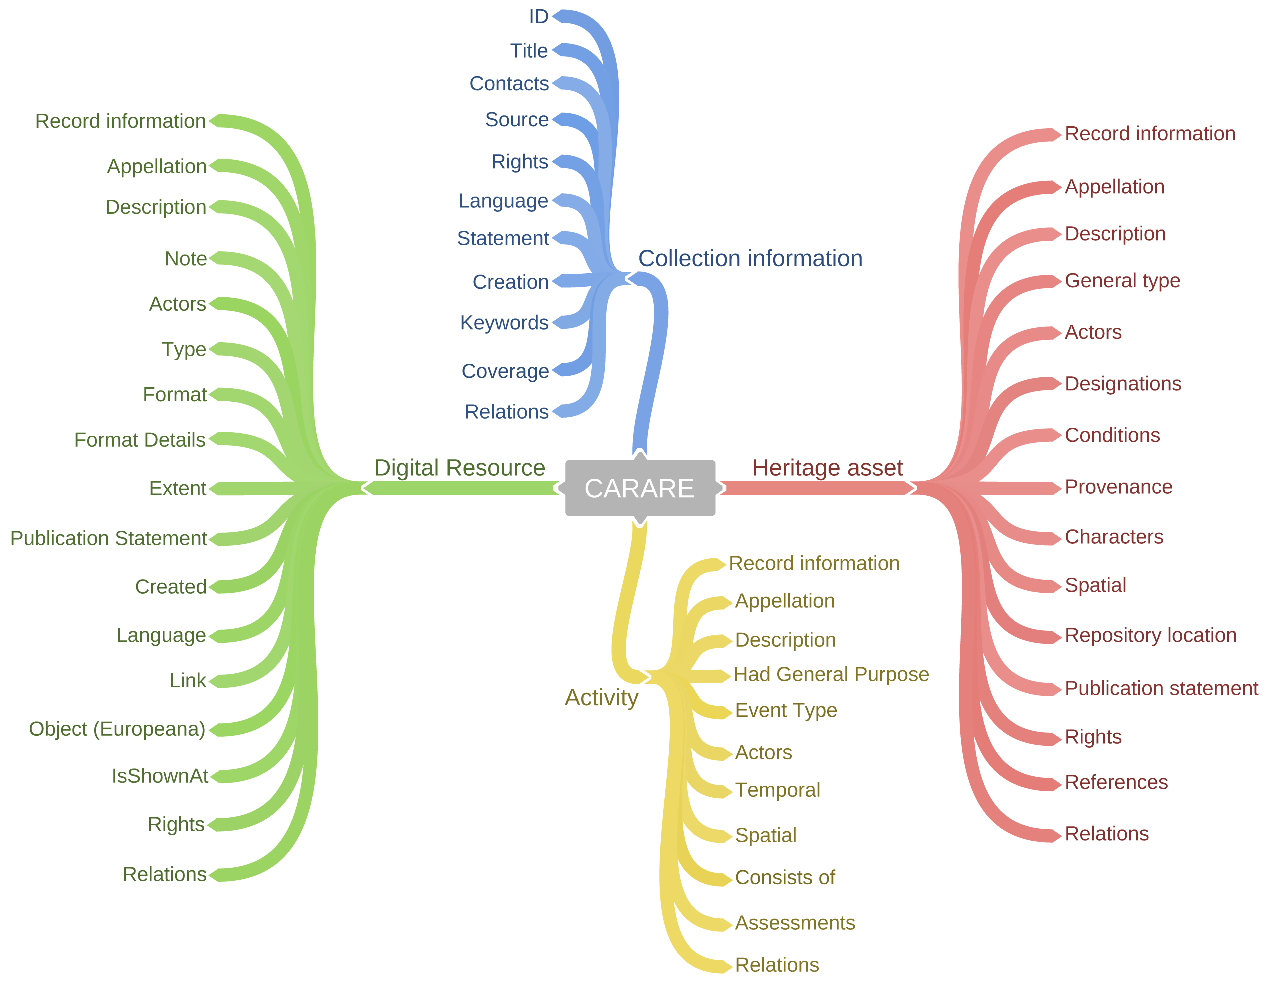
\includegraphics[width=0.9\textwidth]{bilder/doku_CARARE}
		\end{center}
		\caption{CARARE 2.0. (Grafik erstellt mit coggle.it.)}
		\label{abb:doku_CARARE}
\end{figure}
\item Das Metadatenschema von IANUS in Abbildung \ref{abb:doku_IANUS} wurde ebenfalls für Daten aus dem Bereich der Archäologien und Altertumswissenschaften entwickelt und orientiert sich an bereits vorhandenen Standards.
\begin{figure}[h!bt]
		\begin{center}
			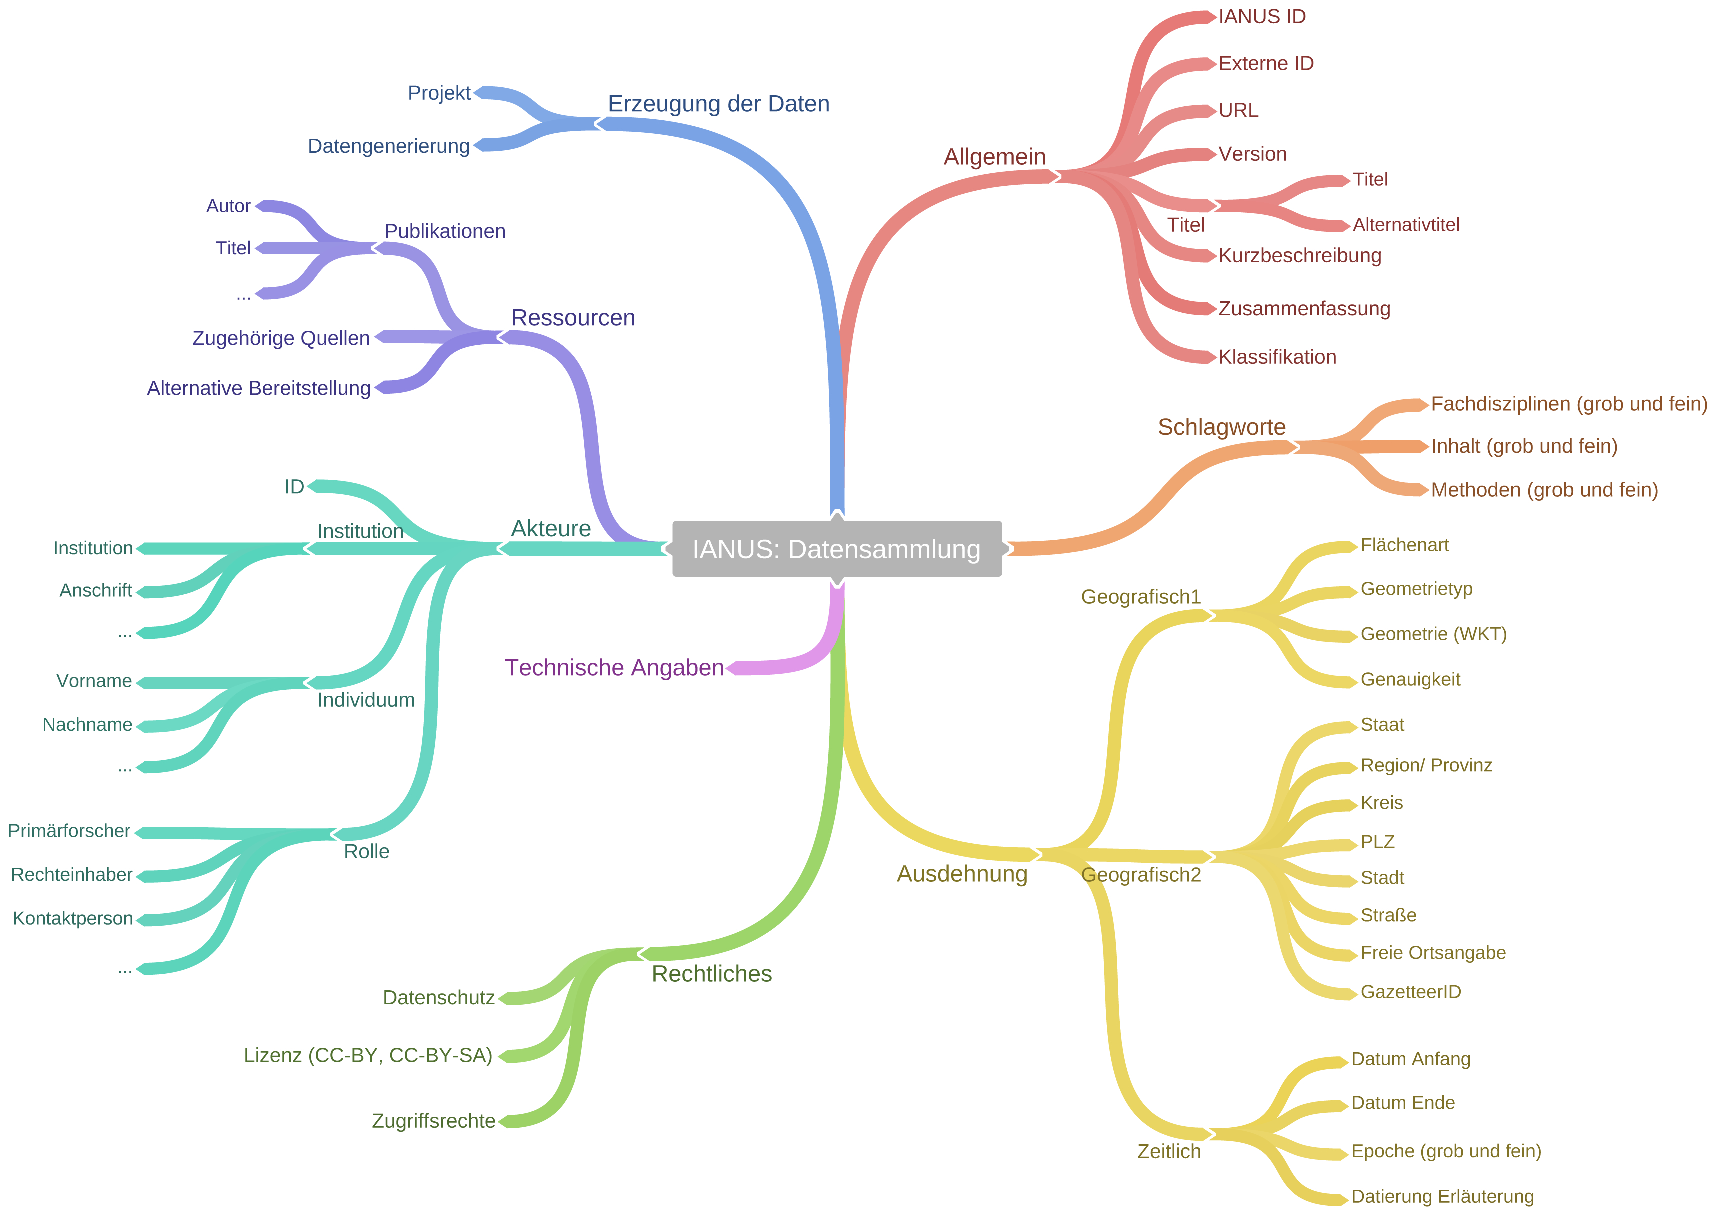
\includegraphics[width=\textwidth]{bilder/doku_IANUS}
		\end{center}
		\caption{Eine vereinfachte Darstellung des Metadatenschemas von IANUS. (Grafik erstellt mit coggle.it.)}
		\label{abb:doku_IANUS}
\end{figure}
\end{itemize}

Darüberhinaus gibt es weitere internationale Standards und institutionelle Vorgaben:
\begin{itemize}
	\item CIDOC Conceptual Reference Modell (CIDOC CRM) wurde von der Arbeitsgruppe "`Dokumentationsstandards"' im Internationalen Komitee für Dokumentation (CIDOC) des internationalen Museumsverbandes (ICOM) erarbeitet. Es dient der Strukturierung und formalen Beschreibung von Informationen, Konzepten und Relationen im Bereich des Kulturerbes. Seit 2006 ist CIDOC CRM unter ISO 21127 standardisiert. Für CIDOC-CRM gibt es zusätzlich die im Rahmen von ARIADNE entwickelten Erweiterungen CRMarchaeo, CRMba, CRNdig und CRMgeo, die eine Relevanz für die Archäologie haben. Sie werden in dem Ariadne Reference Model zusammengefasst.
	\item Das Lightweight Information Describing Objects (LIDO) wurde als Austauschformat für bewegliche Objekte in Museen von Arbeitsgruppen innerhalb von CIDOC entwickelt.
	\item Historic Environment Records oder MIDAS Heritage aus Großbritannien.
	\item Vorgaben verschiedener Denkmalämter. Weitere Informationen dazu sind in dem Abschnitt "`Grabungsdokumentation"' ab Seite \pageref{grabungsdokumentation} zu finden.
\end{itemize}


%##################################################################################

\subsection{Kontrollierte Vokabulare, Thesauri und Normdaten}
Damit Metadaten möglichst sinnvoll genutzt und maschinell verarbeitet werden können, sollten neben klar definierten Metadatenschemata auch möglichst einheitliche Begriffe und homogene Beschreibungen verwendet werden. Nur wenn gleiche Dinge auch mit den gleichen Begriffen benannt werden, ist es möglich vollständige und präzise Suchergebnisse zu erhalten oder vergleichbare Daten richtig miteinander zu verknüpfen. Die Vorgabe und Definition von festen Begriffen und Regeln hilft zudem, Mehrdeutigkeiten und Redundanzen zu vermeiden, etwa wenn eine Zeichenkette verschiedene Bedeutungen besitzen kann (z. B. Abakus als Rechenhilfsmittel oder als architektonischer Abschluss eines Kapitells), ein identischer Sachverhalt durch unterschiedliche Worte erfasst werden kann (z. B. Survey und Oberflächenbegehung) oder die Form der Angabe variieren kann (z. B. ein Datum in der Form 12.03.2012 oder 2012-03-12).
 
Das geeignete Mittel zur Vereinheitlichung der sprachlichen Vielfalt sind sogenannte kontrollierte oder normierte Vokabulare, die entweder einfache Wortlisten oder strukturierte Thesauri sein können, in denen Wörter zusammen mit ihrem semantischen Kontext verwaltet werden. Diese "`terminologische Kontrolle"' kann in unterschiedlicher Weise systematisiert und implementiert sein. 

Beispielsweise können innerhalb eines Projektes alle zu verwendenden Begriffe unter allen Beteiligten abgestimmt, klar fachlich definiert, voneinander abgegrenzt und in strukturierter Form dokumentiert werden. Diese Absprachen können dann in einem zentralen Textdokument als Projektleitfaden abgelegt oder in einer Datenbank als Felder umgesetzt werden, die nur eine begrenze Auswahl von Begriffen zur Beschreibung eines spezifischen Sachverhaltes zulassen (z. B. für das Attribut Filmart nur die Werte "`Diapositiv (Farbe)"', "`Negativfilm (Farbe)"', "`Negativfilm (SW)"' und "`Digital"').

Besser eignen sich jedoch etablierte, standardisierte, globale Vokabulare, Thesauri oder Normdateien. Sie weisen oft eine thematische, fachspezifische oder institutionelle Ausprägung auf und werden von maßgeblichen Einrichtungen kontinuierlich gepflegt. Dazu gehören beispielsweise Normdateien zur Katalogisierung aus dem Bibliotheksbereich, Personennormdateien oder Thesauri zur eindeutigen Identifizierung von geografischen Orten oder Zeitbegriffen. 

Diese globalen Systeme bieten nicht nur eine feste Bezeichnung und eine Definition eines Begriffes oder des diesem zugrunde liegenden Konzeptes, sondern auch alternative und gegebenenfalls mehrsprachige Benennungen und eine eindeutige Kennung zur Identifizierung des Begriffes. So kann beispielsweise der Ort "`Alexandria"' (\href{http://www.geonames.org/361058/alexandria.html}{361058}) in Ägypten von dem Ort "`Alexandria"' (\href{http://www.geonames.org/4744091/alexandria.html}{4744091}) in den USA mittels der in den Klammern angegebenen Kennungen aus GeoNames unterschieden werden.

Bereits existierende Thesauri und Vokabulare sollten bei der Vergabe von Metadaten berücksichtigt und angewendet werden, um den späteren elektronischen Austausch, also die Interoperabilität, der eigenen Daten mit anderen Systemen erheblich zu vereinfachen. Wenn Ressourcen in mehreren Sprachen vorliegen und entsprechend multilingual beschrieben werden sollen, müssen die genutzten Wörterbücher, Thesauri und Schlagwortsysteme äquivalente Begriffe in mehreren Sprachen abbilden.

Für die systematische Erfassung archäologischer und allgemeiner Begriffe existieren folgende Vokabulare:
\begin{itemize}
	\item Art \& Architecture Thesaurus (AAT) wurde Ende der 1970er von dem Getty Research Institute entwickelt, um die Katalogisierungsprozesse in Kunstbibliotheken und im Museumsbereich zu unterstützen und zu vereinheitlichen. Dieser Thesaurus wird von einer breiten Fachgemeinschaft kuratiert.
	\item Heritage Data -- Linked Data Vocabularies for Cultural Heritage führt die in England genutzten Vokabulare im Bereich kulturelles Erbe zusammen. 
	\item Wortnetz Kultur (WNK) wurde vom Landschaftsverband Rheinland ins Leben gerufen, um die Inhalte in deren verschiedenen Informationssystemen zu vereinheitlichen. Mittlerweile sind die Themen Kulturlandschaft, Archäologie, Kulturanthropologie, Denkmalpflege sowie Kunstgeschichte mit rund 15.000 Begriffen vertreten.
	\item Das DAI bietet mit iDAI.vocab (auch archwort) ein flaches multilinguales Vokabular mit Links auf den AAT. Außerdem gibt es mit dem iDAI.the"-sau"-rus ein System, das die Schlagworte aus den unterschiedlichen Thesauri der Bibliotheken zusammenführt und strukturiert.
	\item Die Encyclopedia of Life stellt eine weltweite Datenbank für Pflanzen und Lebewesen dar, die zusätzlich Fotos, Verbreitungskarten und Literaturhinweise enthält.
	\item In Wikidata werden alle strukturierten Daten aus den Systemen von WikiMedia erfasst und mit eindeutigen Identifikatoren zur Verfügung gestellt.
\end{itemize}

Für die eindeutige Identifizierung von geografischen Orten eignen sich, neben den amtlichen Gemeindekennzahlen und dem geodätischen Parameterdatensatz EPSG, folgende Ortsthesauri, sogenannte Gazetteers:
\begin{itemize}
	\item GeoNames ist ein Gazetteer, in dem vor allem moderne Orte, deren alternative Bezeichnungen und geografischen Koordinaten systematisch erfasst werden. Die Inhalte stammen von engagierten Nutzern weltweit.
	\item Getty Thesaurus of Geographic Names (TGN) wurde 1987 von dem Getty Research Institute ins Leben gerufen, um ebenfalls deren Katalogisierungsprozesse in Kunstbibliotheken und im Museumsbereich zu unterstützen und zu vereinheitlichen.
	\item Das DAI betreibt mit dem iDAI.gazetteer einen Gazetteer für die eindeutige Adressierung von antiken Orten, in dem außerdem auch die Eintragungen in GeoNames berücksichtigt werden.
	\item Pleiades ist ebenfalls ein Gazetteer für antike Orte mit einem Schwerpunkt auf der griechischen und römischen Antike, dessen Inhalt durch jeden Nutzer erweitert oder korrigiert werden kann.
\end{itemize}

Auch für Zeitbegriffe gibt es kontrollierte Vokabulare:
\begin{itemize}
	\item PeriodO ist ein Gazetteer für Zeitepochen. Neben der zeitlichen Information wird auch die geografische Verbreitung der jeweiligen Epoche erfasst.
	\item iDAI.chronontology ist ein vom DAI durchgeführtes Projekt, das wie PeriodO zeitliche und geografische Informationen miteinander in Beziehung setzt.
\end{itemize}

Zur Erfassung von Informationen zu Personen oder Institutionen sollten Normdateien verwendet werden, wie beispielsweise:
\begin{itemize}
	\item Das Virtual International Authority File (VIAF) kombiniert Normdateien mehrerer Nationalbibliotheken und speichert Informationen zu Personen und Institutionen, sowie deren Publikationen.
	\item Die Open Researcher and Contributor ID (ORCID) ist eine alphanumerische Zeichenkette, die der eindeutigen Identifizierung wissenschaftlicher Autoren dient. ORCID wird von einem gemeinnützigen Gremium betrieben und Autoren müssen sich selbst registrieren, um eine ID zu bekommen.
	\item Die Gemeinsame Normdatei (GND) der Deutschen Nationalbibliothek dient primär der Katalogisierung in Bibliotheken. Neben Informationen zu Personen und Körperschaften werden auch weitere Informationen zu Konferenzen, Geografika, Sachschlagwörtern und Werktiteln verwaltet.
\end{itemize}

Wenn in Metadaten auf Publikationen verwiesen werden soll, eignen sich folgende Systeme:
\begin{itemize}
	\item Die Internationale Standardbuchnummer (engl. \emph{International Standard Book Number}, ISBN) wird zur eindeutigen Identifizierung von Publikationen verwendet. Sie ist vor allem im Buchhandel verbreitet. Für Reihen und Zeitschriften wird eine ähnliche Nummer, die ISSN (Internationale Standardnummer für fortlaufende Sammelwerke, engl. \emph{International Standard Serial Number}) verwendet.
	\item Für in Deutschland veröffentlichte Medienwerke gibt es eine Ablieferungspflicht bei der Deutschen Nationalbibliothek, weshalb die dort vergebenen  eindeutigen Kennungen ebenfalls zur Identifizierung verwendet werden können.
	\item Für archäologische und altertumswissenschaftliche Publikationen eignen sich auch die Identifikatoren aus iDAI.bibliography (Zenon), in dem die umfangreichen Bestände aller DAI Bibliotheken nachgewiesen werden.
\end{itemize}

%##################################################################################
\label{metadatenSpeicherung}
\subsection{Speicherung von Metadaten}
Für eine strukturierte Speicherung von Metadaten gibt es verschiedene Möglichkeiten und Wege, die einerseits von dem Zeitpunkt (synchron mit der Datenerhebung oder im Nachhinein) und andererseits von der Art der Metadatenerfassung (manuell oder automatisiert) abhängen. 

Grundsätzlich sollten Metadaten so früh wie möglich, also bereits bei der Generierung von neuen digitalen Objekten oder am Anfang eines neuen Forschungsvorhabens vergeben werden, auch wenn diese noch nicht vollständig angegeben werden können. Somit wird vermieden, dass Informationen im Nachhinein nicht mehr nachgetragen werden können, da sie vergessen wurden oder sich nicht mehr ermitteln lassen. Eine regelmäßige Aktualisierung und kontinuierliche Metadatenpflege ist ratsam und für manche Daten, wie etwa 3D-Scans oder Geodaten auch erforderlich.

Abhängig vom verwendeten Dateiformat können Metadaten auch direkt in eine Datei integriert werden. Dies kann teilweise automatisiert erfolgen, wie beispielsweise bei digitalen Fotos. Hier werden von der Kamera automatisch technische Angaben zu Dateiformat, Verschlusszeit, Blendenöffnung, Farbinformationen usw. direkt in der Bilddatei hinterlegt. Je nach Gerät können über die Voreinstellungen auch deskriptive Informationen wie Fotograf, Aufnahmedatum, Land etc. hinzugefügt werden. Ähnliche Verfahren zur automatischen Metadatenerzeugung sind auch bei Vermessungsgeräten üblich. Die durch Geräte generierten Metadaten werden unmittelbar in einem besonderen Bereich und auf standardisierte Weise in der resultierenden Datei gespeichert, etwa bei Fotos im Format Exif im Header der Datei.

Mit Hilfe von editierbaren Dateieigenschaften können auch in anderen Dateiformaten, wie etwa DOCX, ODT oder PDF, Metadaten direkt im Header gespeichert werden. Dabei ist jedoch eine manuelle Eingabe mit Hilfe der passenden Software erforderlich. Diese Informationen können über die Eigenschaften einer Datei angezeigt und teilweise verändert und ergänzt werden, was in Abbildung \ref{eigenschaftenAcrobat} für ein PDF-Dokument zu sehen ist. Bei der Auswahl von Anwendungen sollte darauf geachtet werden, ob diese spezifischen Metadaten entweder als separate Datei exportiert oder ob sie mit den Dateien, in denen sie enthalten sind, auch unabhängig von der ursprünglichen Software geöffnet werden können.

\begin{figure}[t!]
  \begin{center}
    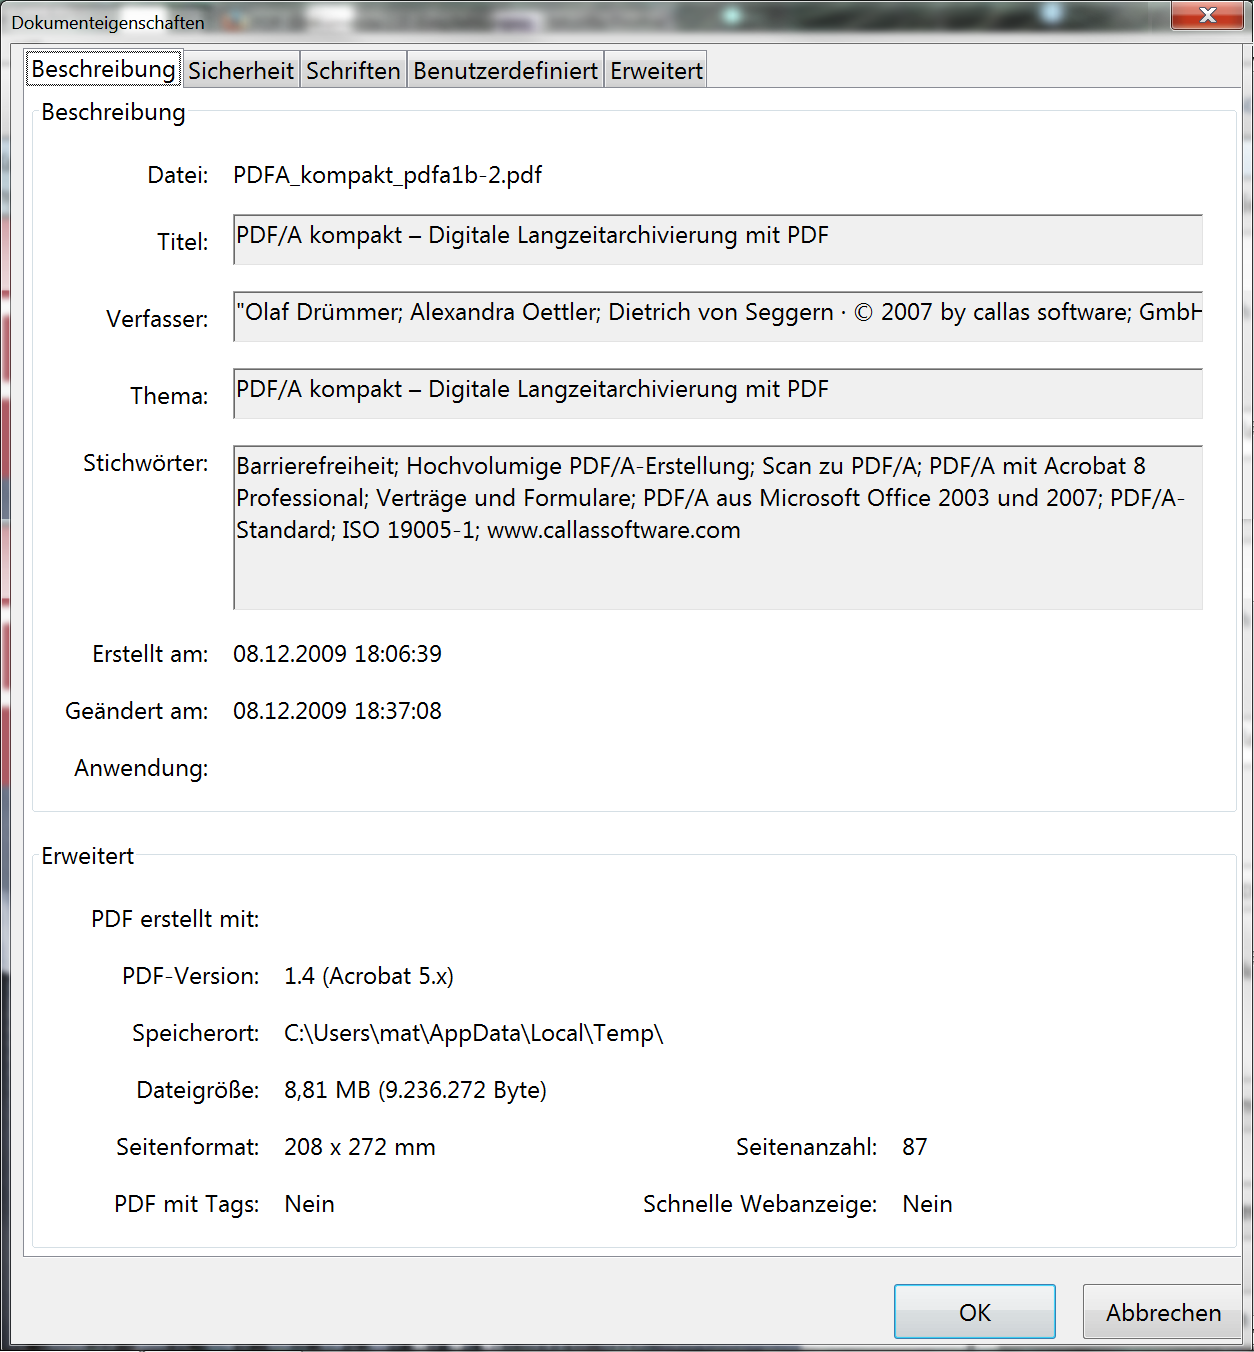
\includegraphics[width=0.9\textwidth]{bilder/doku_AdobeEigenschaften}
  \end{center}
  \caption{Beispiel der Metadaten eines PDF-Dokumentes im Programm Adobe Reader. Die Metadaten können unter "`Datei > Eigenschaften"' angezeigt und verändert werden.}
  \label{eigenschaftenAcrobat}
\end{figure}

Bei textbasierten (insbesondere XML-basierten) Dateiformaten oder Textdateien, die Auszeichnungssprachen verwenden (wie etwa SVG-, HTML- oder XML-Dateien), können Metadaten leicht mittels Auszeichnungselementen im Header der Datei integriert werden. Konkrete Hinweise für die Bearbeitung und Ergänzung von Metadaten für bestimmte Dateiformate sind in den entsprechenden Abschnitten im Kapitel Dateiformate ab Seite \pageref{dateiformate} zu finden. Auch Hinweise für die Extraktion von Metadaten in separate Dateien sind ebenfalls in den entsprechenden Abschnitten zu finden.

Für Dateiformate, in denen kein eigener Metadatenbereich vorgesehen ist, oder für übergeordnete projekt- und methodenbezogene Metadaten, ist eine Speicherung in separaten Dateien oder Systemen erforderlich. Hierfür eignen sich Tabellen und Datenbanken, da diese die Erfassung mithilfe spezifischer Eingabemasken, einer gezielten Suche und einer strukturierten Sicherung von Metadaten erleichtern. Zusätzlich erlauben sie eine (Teil-)Automatisierung der Metadaten, wie etwa die automatische Speicherung des Datums der letzten Bearbeitung eines Datensatzes und den Namen des Bearbeiters. Ein weiterer Vorteil der Erfassung von Metadaten in Tabellen oder Datenbanken besteht in der effizienten Bearbeitung von Merkmalen, die für mehrere Dokumente identisch sind, wie beispielsweise der gleiche Maßstab für alle Zeichnungen eines Projektes.

Bei der Speicherung von Metadaten in separaten Dateien muss in besonderer Weise darauf geachtet werden, dass die Beziehungen zwischen beiden Einheiten eindeutig und aktuell sind. Wird etwa bei den Metadaten der Name einer Datei zur Identifizierung verwendet, muss sichergestellt werden, dass dieser einmalig ist (ggf. in Kombination mit seinem Speicherort) und dass im Falle der Umbenennung der Datei der Eintrag auch bei den Metadaten aktualisiert wird.

Die Erfassung von Metadaten in einer Freitextdatei sollte vermieden werden, da diese meist nicht automatisiert durch Computer überprüft und verarbeitet werden können.

Bei Dokumenten mit Textinhalt können beschreibende Metadaten auch automatisch erzeugt werden, indem nach charakteristischen Zeichenketten gesucht wird und Schlag- und Stichworte extrahiert werden. Allerdings reicht die Qualität einer automatischen Erschließung bislang nicht an eine manuelle und intellektuelle Metadatenvergabe heran, da maschinell nicht nur sinnvolle Deskriptoren herausgefiltert werden.

Für die Übergabe von Dateien und Metadaten an ein Langzeitarchiv gilt die Empfehlung, die Metadaten sowohl in den Originaldateien selbst als auch in einem separaten, strukturierten und textbasierten Dokument vorzuhalten: in den Originaldateien selbst, um keine verwaisten, also undokumentierten Werke zu erzeugen, und als separate Textdatei, um eine automatisierte Verarbeitung und den Austausch von Referenzangaben zu vereinfachen.
\subsection{Metadaten in der Anwendung}
\label{Metadaten-anwendung}
\paragraph{Projektbezogene Metadaten}
Die wichtigsten Metadaten, die für die Beschreibung eines Projektes oder einer Dokumentensammlung erforderlich sind, werden in der folgenden Tabelle abgebildet und knapp definiert. Sie geben einen Überblick über einen größeren, zusammenhängenden Datenbestand und beschreiben den fachlichen Kontext in dem dieser entstanden ist. Vergleichbar einem Bibliothekskatalog liegt die Hauptfunktion dieser Metadaten darin, dass externe Personen ein Projekt oder eine dessen digitale Daten über Web-Portale und Suchmaschinen finden und einordnen können. Darüber hinaus enthalten sie rechtliche Informationen, die für den weiteren Umgang mit den Daten wichtig sind. 

Die hier vorgestellten Eigenschaften basieren auf dem Dublin Core Metadata Schema und den Angaben, wie sie vom ADS in den UK und tDAR in den USA erhoben werden, um einen zukünftigen Austausch zu vereinfachen. Ein darauf aufbauendes ausführliches Metadatenschema, das auch die Grundlage für die Archivierung von Projektdaten bei IANUS bildet, sowie ausgefüllte Beispielformulare sind in dem Kapitel Archivierung von Forschungsdaten in IANUS ab Seite \pageref{archivierungIANUS} zu finden.

\begin{center}
	\begin{longtable}{L{0.25\textwidth} p{0.68\textwidth}}
		\toprule
		Bezeichnung & Kurzdefinition\\ \midrule \endfirsthead
		\multicolumn{2}{l}{\footnotesize Fortsetzung der vorhergehenden Seite}\\
		\toprule
		Bezeichnung & Kurzdefinition\\ \midrule \endhead
		\bottomrule \multicolumn{2}{r}{{\footnotesize Fortsetzung auf der nächsten Seite}} \\
		\endfoot
		\bottomrule 
		\endlastfoot

		Identifizierung -- Projekttitel & Verbindliche Kurzbezeichnung des Projektes.\\
		Identifizierung -- Alternativtitel & Ggf. alternative Titel für ein Projekt.\\
		Identifizierung -- Projektnummer(n) & Nummern oder Kennungen, die z.B. innerhalb der durchführenden Organisation oder von Mittelgebern verwendet werden, um das Projekt eindeutig identifizieren zu können.\\
		Kurzbeschreibung & Knappe Angaben zur Fragestellung, zum Verlauf und Ergebnis des Projektes sowie Skizzierung der Datensammlung (insgesamt ca. 100-300 Worte)\\
		Schlagworte -- Fachdisziplinen & Stichworte, die die beteiligten Disziplinen und Fächer benennen. Sofern die Stichworte auf publizierten Standards oder internen Thesauri beruhen, müssen diese mitangegeben werden.\\
		Schlagworte -- Inhalt & Stichworte, die den Inhalt der Datensammlung benennen., z. B. zu Materialgruppen, Fundstellen-Klassifizierung, Quellenarten,  Kulturgruppen etc. Sofern die Stichworte auf publizierten Standards oder internen Thesauri beruhen, müssen diese mitangegeben werden.\\
		Schlagworte -- Methoden & Stichworte, die die eingesetzten Forschungsmethoden beschreiben. Sofern die Stichworte auf publizierten Standards oder internen Thesauri beruhen, müssen diese mitangegeben werden.\\
		Ausdehnung -- Geografisch-1 & Detaillierte Angaben zur räumlichen Ausdehnung oder zum Fundort des untersuchten Gegenstandes mittels geografischer Koordinaten. Die maximale Ausdehnung kann als Bounding Box angegeben werden.\\
		Ausdehnung -- Geografisch-2 & Sprachliche Beschreibung des untersuchten Gegenstandes mittels Ortsangaben mit Land, Stadt, Kreis, Straße, Gemarkung etc. Sofern Namen sich im Lauf der Zeit geändert haben, dies gesondert vermerken. Sofern eine Referenz zu einer Geo-Ressource oder einem Gazetteer existiert, sollte diese ebenfalls angegeben werden.\\
		Ausdehnung -- zeitlich & Chronologische Angaben zum untersuchten Gegenstand, entweder als Periodenbezeichnung und/oder mit groben/genauen Jahresangaben. Sofern die Stichworte auf publizierten Standards oder internen Thesauri beruhen, müssen diese mitangegeben werden.\\
		Primärforscher -- Person & Personen, die entweder für das Projekt als Ganzes, für das Datenmanagement oder für die Erzeugung bestimmter Datenarten zentral bzw. verantwortlich sind. Hier ist eine Kontaktadresse erforderlich und die aktuelle/letzte institutionelle Zugehörigkeit, damit die Personen bei Rückfragen erreicht werden kann.\\
		Eigentümer -- Organisation & Organisation, der die unter "`Primärforscher"' genannten Personen angehören, oder die nach Ausscheiden derselben für die Daten verantwortlich ist, im weitesten Sinne also Eigentümer der Daten ist. Hier ist eine Kontaktadresse erforderlich, damit die Organisation bei Rückfragen erreicht werden kann.\\
		Finanzierung & Nennung der Organisation(en) / (Dritt-)Mittelgeber, durch die das Projekt finanziert wurde. Es sollte jeweils der Zeitraum der Finanzierung angegeben werden.\\
		Veröffentlichung -- Projektdaten & Wenn die hier beschriebene Datensammlung des Projektes bereits an anderer Stelle veröffentlicht / online gestellt wurde, bitte entsprechende Angaben machen, z. B. durch Nennung der Organisationen, Datenarchive, Online-Ressourcen etc.\\
		Veröffentlichung -- Ergebnisse & Analoge oder digitale Publikationen zu Ergebnissen des Projektes oder zur Datensammlung des Projektes, ausführliche bibliographische Angaben (ohne fachspezifische Abkürzungen) unter Nennung des Verlages erforderlich.\\
		Dauer -- Projekt & Anfangs- und Enddatum des Projektes.\\
		Dauer -- Datenbestand & Anfangs- und Enddatum der Erzeugung oder Verarbeitung digitaler Daten im Rahmen des Projektes.\\
		Rechtliches -- Urheberrechte & Name des Inhabers der Urheber-, Nutzungs- und Verwertungsrechte; i. d. R. die Organisation, an der der Primärforscher beschäftigt war.\\
		Rechtliches -- Lizenzgeber & Angabe der Person, die i. d. R. als Vertretung für eine Organisation für die Lizenzierung von Daten zur Nachnutzung verantwortlich und berechtigt ist, einen Datenübergabevertrag abzuschließen.\\
		Rechtliches -- Datenschutz & Angaben, ob in der Datensammlung datenschutzrelevante Informationen enthalten sind. Wenn ja, in welchem Umfang.\\
		Quellen -- Ältere & Ältere Quellen oder existierende Ressourcen, auf denen die Daten aufbauen.\\
		Quellen -- Zugehörige & Sofern während des Projektes Informationen, Datensammlungen, (un-)publizierte Dokumente, Online-Ressourcen etc. verwendet oder erzeugt wurden, die nicht Teil der hier beschriebenen Datensammlung sind, aber für deren Verständnis wichtig sind, bitte entsprechende Angaben zu Art und Umfang dieser Quellen machen.\\
		Sprache & Die in den Dokumenten und Dateien verwendete(n) Sprache(n). Sprachkennungen nach ISO 639 angeben.\\
		Art der Daten & Kurzcharakterisierung der Daten, z. B. ob es sich um Rohdaten, verarbeitete Daten, Interpretationen, Ergebnisse, Abschlussberichte etc. handelt.\\
		Vollständigkeit & Aussagen zur Vollständigkeit der Projektdaten, z. B. ob bestimmte Datenarten noch fehlen und warum.\\
		Dateiformate & Auflistung der Dateiformate, die in der Datensammlung vorkommen, ggf. unter Nennung der verwendeten Programme und Zeichenkodierungen.\\
		Zugriffsrechte & Festlegung der gewünschten Zugriffsrechte für die Daten, sofern diese für den gesamten Projekt-Datenbestand gelten sollen; differenzierte Regelungen müssen auf Dateiebene vorgenommen werden.\\
		Signatur Metadaten & Angabe darüber, wer die o. g. Metadaten wann ausgefüllt hat.\\
		\bottomrule
	\end{longtable}
\end{center}

\paragraph{Dateibezogene Metadaten}
Bei dieser Art von Metadaten handelt es sich um technische und inhaltliche Informationen, die Nutzern verständlich machen, wie einzelne Dateien innerhalb eines Projektes oder einer Datensammlung beschaffen sind und welche Möglichkeiten der Nachnutzbarkeit sie beinhalten. 

Dateibezogene Metadaten sind abhängig von dem Format, dem Inhalt und der Methode, mit denen die Dateien erzeugt wurden. Beispielsweise sind für Rastergrafiken, die durch digitale Fotografie entstanden sind, andere Angaben erforderlich (Fotograf, Aufnahmedatum, Aufnahmeort, abgelichtetes Objekt etc.) als für Rasterdateien, die durch geophysikalische Messungen erzeugt wurden (Koordinaten, Messgerät, Genauigkeit, Datum etc.). Zusätzliche spezifische Angaben, die für bestimmte Dateiformate empfohlen werden, sind in den verschiedenen Kapiteln zu den jeweiligen Formaten ab Seite \pageref{dateiformate} beschrieben.

Es gibt jedoch dateibezogene Metadaten, die unabhängig von Format, Inhalt und Methode für alle Einzeldateien gleichermaßen relevant und notwendig sind. Zu diesen Metadaten gehören neben den Angaben zu Dateiname, Dateiformat, Dateiversion, Titel, Beschreibung und Ersteller auch Informationen zur verwendeten Soft- und Hardware, Versionierung, zu rechtlichen Aspekten und Verweise auf weitere relevante Dateien.

Auch wenn es in der Theorie wünschenswert ist, diese Angaben sowie die zugehörigen spezifischen Angaben zu Methoden und Dateiformaten für jede Datei einzeln zu erfassen, so zeigt die Praxis, dass es häufig ausreichend ist, einen Metadatensatz für Gruppen von Dateien anzulegen, wenn diese das gleiche Format oder die gleichen inhaltlichen Eigenschaften aufweisen. 

\begin{center}
	\begin{longtable}{L{0.25\textwidth} p{0.68\textwidth}}
		\toprule
		Bezeichnung & Kurzdefinition\\ \midrule \endfirsthead
		\multicolumn{2}{l}{\footnotesize Fortsetzung der vorhergehenden Seite}\\
		\toprule
		Bezeichnung & Kurzdefinition\\ \midrule \endhead
		\bottomrule \multicolumn{2}{r}{{\footnotesize Fortsetzung auf der nächsten Seite}} \\
		\endfoot
		\bottomrule 
		\endlastfoot
		
		Identifikator, Dateiname & Eindeutiger Name der Datei.\\
		Dateiformat & Format, in dem die Datei abgespeichert ist.\\
		Urheber & Name des Verfassers oder Erstellers der Datei.\\
		Titel & Titel der Datei, nicht der Dateiname.\\
		Beschreibung & Beschreibung des Inhalts der Datei. \\
		Schlagworte & Schlagworte, wie etwa Periode, Fundstelle oder charakteristische Merkmale. Wenn vorhanden, angemessene Thesauri verwenden.\\
		Software -- Dateierstellung & Software, mit der die Datei erstellt wurde.\\
		Hardware -- Dateierstellung & Hardware, mit der die Datei erstellt wurde, v. a. bei technischen Geräten wie Kameras, GPS-Geräten, Vermessungsinstrumenten, Laserscanner etc.\\
		Betriebssystem -- Dateierstellung & Betriebssystem, das verwendet wurde als die Datei erstellt wurde.\\
		Erstellungsdatum & Datum, an dem die Datei erstellt wurde. Datum und Zeit in UTC nach ISO 8601.\\
		Letzte Aktualisierung & Datum, an dem die Datei zuletzt bearbeitet wurde. Datum und Zeit in UTC nach ISO 8601.\\
		Dateiversion & Angabe der Versionsnummer der Datei.\\
		Weitere Dateien & Referenzen auf Dateien, die für das Verständnis einer anderen Datei zentral sind, insbesondere für zusammenhängende, komplexe Dateien oder wenn auf eine Ursprungsdatei verwiesen werden soll.\\
		Sprache & Sofern schriftliche Inhalte vorhanden sind, die Sprache angeben. Sprachkennungen nach ISO 639 angeben.\\
		Copyright-Angaben & Angaben zur Person oder Einrichtung, die das Copyright oder die Lizenzrechte an der Datei oder deren Inhalt besitzt.\\
		\bottomrule
	\end{longtable}
\end{center}

\paragraph{Methodenbezogene Metadaten}
Jede Fachdisziplin innerhalb der Altertumswissenschaften verfügt über spezifische Forschungsmethoden. Auch diese haben Einfluss auf Umfang, Art, Struktur und Inhalt digitaler Objekte, da sie bei verschiedenen Arbeitsweisen und technischen Geräten unterschiedlich ausfallen. Daher sollten methodenbezogene Metadaten ebenfalls dokumentiert werden, insbesondere wenn mehrere Zwischenstände einer Prozesskette archiviert und Dritten zur Verfügung gestellt werden sollen. Je nach Genauigkeit der Methodenbeschreibung kann sie sich sowohl auf eine Einzeldatei als auch auf mehrere Dateien gleichen Typs beziehen.

Die Angabe der methodenbezogenen Metadaten ist wichtig, um zu beschreiben, wie die Rohdaten in prozessierte Daten überführt wurden. Außerdem kann so verstanden werden, welchen Einfluss die angewandte Methode auf das Ergebnis hat, das Ergebnis folglich zu interpretieren ist und wo Fehler zu erwarten sind.

Zusätzliche spezifische Angaben, die für bestimmte Forschungsmethoden oder Prozesse empfohlen werden, sind in den einzelnen Kapiteln des Abschnittes Forschungsmethoden ab Seite \pageref{methoden} beschrieben.

\begin{center}
	\begin{tabular}{L{0.25\textwidth} p{0.68\textwidth}}
		\toprule
		Bezeichnung & Kurzdefinition\\ \midrule
		Prozessnummer & Eindeutige Nummer eines Prozesses oder einer Methode.\\
		Prozessbeschreibung & Beschreibung des Prozesses oder der Methode. Insbesondere Beschreibung der Ausgangssituation und der Zielvorstellung.\\
		Ausgangsformat(e) & Format der Dateien, die am Anfang eines gesamten Prozesses stehen und den Ausgangspunkt bilden.\\
		Zwischenformat(e) & Format der Dateien, die im Verlauf eines Prozesses erzeugt werden und den Ausgangspunkt für weitere Prozesse bilden.\\
		Zielformat(e) & Format der Dateien, die am Ende eines Prozesses erzeugt werden.\\
		Durchführender & Person(en), die den Prozess durchgeführt hat (haben).\\
		Prozessbeginn & Datum, an dem der Prozess begonnen wurde. Datum und Zeit in UTC nach ISO 8601.\\
		Prozessende & Datum, an dem der Prozess beendet wurde. Datum und Zeit in UTC nach ISO 8601.\\
		Software & Software, mit der der Prozess durchgeführt wurde.\\
		Hardware & Hardware, auf der der Prozess durchgeführt wurde.\\
 		\bottomrule
		\bottomrule
	\end{tabular}
\end{center}


%##################################################################################
\label{grabungsdokumentation}
\subsection{Grabungsdokumentation}
Speziell für die Dokumentation von Grabungen und anderen archäologischen Maßnahmen sind weitere Metadaten erforderlich, die in der folgenden Tabelle aufgelistet sind. Dabei sollten auch die verschiedenen angewandten Methoden berücksichtigt werden, da diese ebenfalls den Umfang und die Art der Dokumentation beeinflussen. Wichtig bei einer Grabungsdokumentation ist, dass nicht nur die digitalen Daten, sondern auch die analogen Daten mit einer Dokumentation versehen sind, um beispielsweise auch Abhängigkeiten zwischen den verschiedenen Daten festzuhalten. Zum Beispiel sollten Zeichnungen mit den Befundbeschreibungen, Fotos mit den Fundstellenplänen oder Objektbeschreibungen mit den jeweiligen Objekten verknüpft sein.

\begin{center}
	\begin{longtable}{L{0.25\textwidth} p{0.68\textwidth}}
		\toprule
		Bezeichnung & Kurzdefinition\\ \midrule \endfirsthead
		\multicolumn{2}{l}{\footnotesize Fortsetzung der vorhergehenden Seite}\\
		\toprule
		Bezeichnung & Kurzdefinition\\ \midrule \endhead
		\bottomrule \multicolumn{2}{r}{{\footnotesize Fortsetzung auf der nächsten Seite}} \\
		\endfoot
		\bottomrule 
		\endlastfoot

		Fundstellenart & Angabe über die Art der Fundstelle. Mehrfachangaben sind möglich, wenn beispielsweise ein sich mit einer Siedlung überlagerndes Gräberfeld beschrieben werden soll.\\
		Maßnahmenart & Angabe über die Art der Untersuchung. Werte können beispielsweise sein: Ausgrabung, Survey, Baustellenbegleitung etc.\\
		Anlass & Angabe des Anlasses, der zur Durchführung der Maßnahme führt. Werte können beispielsweise sein: Rettungsgrabung, Notgrabung, Forschungsgrabung, Lehrgrabung etc.\\
		Grabungsmethodik & Angabe der angewandten Grabungsmethodik. Werte können beispielsweise sein: Flächengrabung, Schichtengrabung, Wheeler-Kenyon-Methode etc.\\
		Verfahren & Angabe über die angewandten Arbeitsverfahren, die nicht zu Dokumentationsverfahren gehören. Werte können beispielsweise sein: Schlämmen, Bohrung, Sieben etc.\\
		Datierung & Datierung der Fundstelle, beispielsweise anhand des archäologischen Fundmaterials. Eingruppierung in eine Epoche als relative Zeitstellung und optional als absolute Zeitangabe. Bei mehrphasigen Fundstellen werden mehrere Zeiträume angegeben.\\
		Fundstellenstatus & Angaben zum Schutzstatus einer Fundstelle.\\
		Bodenbeschaffenheit & Angabe über die natürlichen Gegebenheiten und die Bodenbeschaffenheit, die Einfluss auf die Erhaltungsbedingungen von Objekten und Strukturen haben. Werte können beispielsweise sein: Feuchtboden, Mineralboden, Unter Wasser etc.\\
		Strukturen & Verschlagwortung von aufgefundenen archäologischen Strukturen, die sich aus den Befunden ergeben.\\
		Funde & Verschlagwortung von signifikanten Fundgattungen.\\
		Richtlinie & Angaben zur Grabungs- oder Dokumentationsrichtlinie, die für die Maßnahme vorgegeben war oder gewählt wurde.\\
		Dokumentationssystem & Angabe des verwendeten Dokumentationssystems. Werte können beispielsweise sein: Stellenkartensystem, Single Context Recording, spezielle institutionelle Systeme etc.\\
		Dokumentationsmethoden & Angabe der verwendeten Dokumentationsmethoden. Werte können beispielsweise sein: Text, Foto, Zeichnung, 3D-Scan, Vermessung etc. \\
		\bottomrule
	\end{longtable}
\end{center}

Die große Zahl an Dokumentationsverfahren und Forschungsmethoden führt dazu, dass eine umfassende Grabungsdokumentation aus einer großen Menge unterschiedlicher Dokumente besteht, die folgendes enthalten sollte:
\begin{itemize}
	\item Allgemeine Angaben
	\item Grabungsplan
	\item Grabungstagebuch und Grabungsprotokoll
	\item Befundblätter und Befundliste
	\item Fundzettel und/oder Fundmeldung
	\item Fund- und Probenliste
	\item Datenbanken
	\item Dokumentation der angewandten Methoden, wie:
	\begin{itemize}
		\item Vermessungsmethoden
		\item Fotografie
		\item Photogrammetrie
		\item 3D-Scans
		\item Luftbildaufnahmen
		\item Naturwissenschaftliche Beprobung
		\item Zeichnung
		\item Allgemeine Beschreibungen
	\end{itemize}
	\item Abschlussbericht
\end{itemize}

Wie eine Grabungsdokumentation aussehen und welchen Umfang sie haben soll, wird in zahlreichen Richtlinien und Vorgaben spezifiziert, die bei der Planung des Vorhabens bereits berücksichtigt werden sollten. Dabei handelt es sich meist um Vorgaben von Landesdenkmalämtern. Online verfügbare Vorgaben sind bei den weiterführenden Informationen unter Vorgaben zur Grabungsdokumentation ab Seite \pageref{Metadaten-ListeLDA} aufgelistet.

Um die Grabungsdokumentation zu erleichtern und auch sicher zu stellen, dass alle erforderlichen Metadaten angegeben werden, sollten Vorlagen für Formulare und Checklisten bereits vor der Durchführung der Maßnahme erstellt werden. In der online verfügbaren Fassung der IT-Empfehlungen sind zu diesem Kapitel passende Vorlagen zur freien Verwendung zu finden. Darunter befinden sich eine Befundliste, eine Fotoliste, eine Fundliste, eine Geräteliste, ein Probenverzeichnis, ein Restaurierungsverzeichnis, ein Zeichnungsverzeichnis und ein Dokument zur Urheberrechtsverwaltung. Ein weiterer Anhaltspunkt sind die bereits genannten Richtlinien, sowie das Werk "`Tabellen und Tafeln zur Grabungstechnik"' von Andreas Kinne und das Grabungstechnikerhandbuch des Verbandes der Landesarchäologen. 
\newpage
\subsection{Weiterführende Informationen}
\begin{flushleft}
\quelltyp{Metadaten allgemein}
Archaeology Data Service: Guides to Good Practice -- Project Metadata \urllist{http://guides.archaeologydataservice.ac.uk/g2gp/CreateData\_1-2}

Archaeology Data Service: Project metadata for the Archaeology Data Service \urllist{https://archaeologydataservice.ac.uk/resources/images/attach/ADS_collection_level_metadata_example.pdf}

DARIAH-DE (Hrsg.) Daten- und Metadatenformate in den Fachdisziplinen. Archäologie (2015) \urllist{http://dev2.dariah.eu/wiki/pages/viewpage.action?pageId=20058856}

Deutsche Initiative für Netzwerkinformation e. V. (Hrsg.) Kompetenzzentrum Interoperable Metadaten (KIM) \urllist{http://www.dini.de/ag/standards/}

Gesis: Dokumentation und Metadaten \urllist{https://web.archive.org/web/20150928031540/http://www.gesis.org/archive-and-data-management-training-and-information-center/forschungsdatenmanagement/dokumentation-und-metadaten/}

U. Jensen -- A. Katsanidou -- W. Zenk-Möltgen, Metadaten und Standards, in: S. Büttner -- H.-C. Hobohm -- L. Müller (Hrsg.) Handbuch Forschungsdatenmanagement (Bad Honnef 2011) 83-100 \urllist{http://www.forschungsdatenmanagement.de/?page_id=2}

A. Kinne, Tabellen und Tafeln zur Grabungstechnik (Dresden 2013)\abstand

J. M. Lill, Kontrolliertes Vokabular. Wieso? Weshalb? Warum?, Fachgruppe Dokumentation im DMB: Terminologie -- das Schweizer Messer der Dokumentation (9. Mai 2012, Kunstmuseum Stuttgart) \urllist{http://swop.bsz-bw.de/volltexte/2012/1002/pdf/Lill_Textfassung_VortragDMB2012.pdf}

J. Lindenthal, Normen und Standards für Thesauri (2015) \urllist{https://www.ianus-fdz.de/it-empfehlungen/sites/default/files/NormenEmpfehlungenEntwicklungThesauri_Lindenthal.pdf}

nestor (Hrsg.) Standardisierung -- Metadaten \urllist{https://wiki.dnb.de/display/NESTOR/Metadaten}

C. Papatheodorou -- D. Gavrilis -- K. Fernie -- H. Wright -- J. Richards -- P. Ronzino -- C. Meghini, D3.1 Initial Report on the project registry (2013)\urllist{http://ariadne-infrastructure.eu/Resources/D3.1-Initial-Report-on-the-project-registry}

National Information Standards Organization (Hrsg.) Understanding Metadata \urllist{http://www.niso.org/publications/press/UnderstandingMetadata.pdf}

J. Riley -- D. Becker, Glossary of Metadata Standards (2010) \urllist{http://jennriley.com/metadatamap/seeingstandards_glossary_pamphlet.pdf}

Verband der Landesarchäologen (Hrsg.) Grabungstechnikerhandbuch \urllist{http://www.landesarchaeologen.de/verband/kommissionen/grabungstechnik/grabungstechnikerhandbuch/}

W3C (Hrsg.) Vocabularies \urllist{http://www.w3.org/standards/semanticweb/ontology}

\quelltyp{Metadatenschemata}
Dublin Core Metadata Initiative: \urllist{http://dublincore.org/}

OASIS (Version 1.3): \urllist{http://oasis.ac.uk/pages/wiki/TECHNICAL\%20INFORMATION}

ADeX -- Standard für den Austausch archäologischer Fachdaten: \urllist{http://www.landesarchaeologen.de/verband/kommissionen/archaeologie-und-informationssysteme/projektearbeitsgruppen/adex/}

CARARE metadata schema: \urllist{http://pro.carare.eu/doku.php?id=support:metadata-schema}

IANUS: \urllist{https://www.ianus-fdz.de/it-empfehlungen/archivierung}

CIDOC Conceptual Reference Model (Vers. 5.0.4): \urllist{http://www.cidoc-crm.org/}

CIDOC-CRM, CRMarchaeo, CRMba, CRNdig und CRMgeo: \urllist{http://www.cidoc-crm.org/collaborations}

Ariadne Reference Model: \urllist{http://www.ariadne-infrastructure.eu/Resources/Ariadne-Reference-Model}

LIDO Lightweight Information Describing Objects: \urllist{http://network.icom.museum/cidoc/working-groups/lido/lido-technical/specification/}

MIDAS Heritage: \urllist{http://heritage-standards.org.uk/midas-heritage/}

\quelltyp{Kontrollierte Vokabulare, Thesauri und Normdaten}
Art \& Architecture Thesaurus (AAT): \urllist{http://www.getty.edu/research/tools/vocabularies/aat/}

Heritage Data -- Linked Data Vocabularies for Cultural Heritage: \urllist{http://www.heritagedata.org/blog/vocabularies-provided/}

Wortnetz Kultur (WNK): \urllist{http://www.digicult-verbund.de/vortraege/2015/WNK_WortnetzKultur_20151110.pdf} \vspace{-0.2cm} \hspace{0.2cm}\url{http://www.lvr.de/de/nav_main/kultur/kulturwissen/digitales_kulturerbe/digitales_kulturerbe_1.jsp}\vspace{0.1cm}

iDAI.vocab: \urllist{http://archwort.dainst.org/}

iDAI.thesaurus: \urllist{http://thesauri.dainst.org/de/hierarchical_concepts.html}  

Encyclopedia of Life: \urllist{http://eol.org/}

Wikidata: \urllist{https://www.wikidata.org/wiki/Wikidata:Main_Page}

GeoNames: \urllist{http://www.geonames.org/}

iDAI.gazetteer: \urllist{https://gazetteer.dainst.org/}

Pleiades: \urllist{https://pleiades.stoa.org/} 

Getty Thesaurus of Geographic Names (TGN): \urllist{http://www.getty.edu/research/tools/vocabularies/tgn/} 

PeriodO: \urllist{http://perio.do/}

iDAI.chronontology: \urllist{http://chronontology.dainst.org/}

Virtual International Authority File (VIAF): \urllist{http://viaf.org/}

Open Researcher and Contributor ID (ORCID): \urllist{https://orcid.org/}

Gemeinsame Normdatei (GND): \urllist{http://www.dnb.de/DE/Standardisierung/GND/gnd_node.html}

Katalog der Deutschen Nationalbibliothek: \urllist{http://www.dnb.de/}

iDAI.bibliography (Zenon): \urllist{https://zenon.dainst.org/}

\label{Metadaten-ListeLDA}
\quelltyp{Vorgaben zur Grabungsdokumentation}
ARCHES: Archäologische Archivierung in Europa: Ein Handbuch (EAC-Guidelindes 1): \urllist{http://www.europae-archaeologiae-consilium.org/eac-guidlines}

Verband der Landesarchäologen: \urllist{www.landesarchaeologen.de/fileadmin/Dokumente/Dokumente_Kommissionen/Dokumente_Grabungstechniker/grabungsstandards_april_06.pdf}

Bayerische Landesamt für Denkmalpflege: \urllist{http://www.blfd.bayern.de/bodendenkmalpflege/service/}\vspace{-0.2cm} \hspace{0.2cm}\url{http://www.blfd.bayern.de/medien/dokuvorgaben_august_2016.pdf}\vspace{0.1cm}

Landesdenkmalamt Berlin: \urllist{http://www.stadtentwicklung.berlin.de/denkmal/landesdenkmalamt/download/neuerscheinungen/grabung_standard.pdf}

Brandenburgisches Landesamt für Denkmalpflege: \urllist{https://www.bldam-brandenburg.de/bodendenkmalpflege}

Archäologisches Museum Hamburg: \urllist{http://amh.de/wp-content/uploads/DokumtationsrichtlinienHamburg.pdf}

Landesamt für Denkmalpflege Hessen: \urllist{https://lfd.hessen.de/sites/lfd.hessen.de/files/content-downloads/hA_Grabungs-Dokurichtlinien_2015.pdf}

Niedersächsisches Landesamt für Denkmalpflege: \urllist{https://www.denkmalpflege.niedersachsen.de/download/110131}

LVR-Amt für Bodendenkmalpflege im Rheinland: \urllist{http://www.bodendenkmalpflege.lvr.de/de/service/grabungsrichtlinien/grabungsrichtlinien_1.html}

Generaldirektion Kulturelles Erbe Rheinland-Pfalz: \urllist{http://download.gdke-rlp.de/archaeologie/richtlinien_ausgrabung.pdf}

Zeichenrichtlinien des Landesamtes für Denkmalpflege und Archäologie Sachsen-Anhalt: \urllist{www.lda-lsa.de/fileadmin/bilder/dienste/redaktion/Zeichenrichtlinie.pdf}

Bundesdenkmalamt Österreich: Richtlinien für Archäologische Massnahmen \urllist{https://bda.gv.at/de/publikationen/standards-leitfaeden-richtlinien/richtlinien-fuer-archaeologische-massnahmen/}

Eine Liste weiterer Richtlinien bei Archäologie Online: \urllist{http://www.archaeologie-online.de/links/236/592/659/index.php} 
\end{flushleft}

\newpage
\section{Dateiverwaltung}\label{dateiverwaltung}
\abschnittsautor{M. Trognitz, F. Schäfer, R. Göldner, T. Schenk}
\hyphenation{
Schnitt-stel-le
}
Der tägliche Umgang mit digitalen Daten wird durch eine effiziente Dateiverwaltung erheblich erleichtert. Aussagekräftige Dateinamen, die auch für Dritte verständlich sind, sorgen dafür, dass die Dateien gefunden und deren Inhalt verstanden wird. Einheitliche Dateinamensstrukturen erhöhen die Lesbarkeit. Die konsequente Einhaltung von Versionierungsangaben sorgt dafür, dass immer mit der richtigen Dateiversion gearbeitet wird und eine selbsterklärende Ordnerstruktur hilft dabei auch in großen Projekten bestimmte Dateien wiederzufinden.

Die Konzipierung der Dateiverwaltung muss schon zu Beginn des Projektes erfolgen, damit die Regeln von Anfang an angewendet werden können. Die Niederschrift der durch Beispiele ergänzten Benennungsregeln und deren Weitergabe dient im laufenden Betrieb als wichtiges Nachschlagewerk für die konsistente und konsequente Einhaltung derselben. Dies ermöglicht eine effizientere Arbeitsweise.

Im laufenden Projektbetrieb sollte die Einhaltung der Benennungsregeln kontrolliert und gegebenfalls angepasst werden.


\subsection{Dateiablage}
Mit Dateiablage ist hier vor allem die Ordnerstruktur gemeint. Für die Benennung der Ordner gelten die gleichen Regeln, wie für die Dateibenennung, die im Abschnitt Dateibenennung ab Seite \pageref{dateibenennung} thematisiert werden. Lediglich die Dateinamenserweiterung wird bei Ordnernamen nicht verwendet. Die Dateiablage sollte selbsterklärend sein und unpräzise Namen wie etwa \emph{"`In Arbeit"'} vermieden werden.

Wichtig ist, dass die Dateiablage logisch und hierarchisch aufgebaut ist, damit andere Nutzer die gewünschten Informationen finden und einordnen können. Dies bedeutet unter anderem, dass die Inhalte und Unterordner auch tatsächlich thematisch in den übergeordneten Ordner hineinpassen. Beispielsweise erwartet man in einem Ordner mit dem Namen \emph{"`Fotos"'} diverse Fotos, die bei einer entsprechenden Menge vielleicht noch auf verschiedene Unterordner, wie zum Beispiel \emph{"`Plana"'} und \emph{"`Profile"'}, verteilt sind.   

Ist aber in dem Ordner \emph{"`Fotos"'} ein Unterordner mit dem Namen \emph{"`Zeichnungen"'} enthalten, in dem verschiedene digitalisierte Zeichnungen abgelegt sind, führt das zu Schwierigkeiten. Der Unterordner wird wahrscheinlich nur schwer wiedergefunden werden, da der Name des übergeordneten Ordners einen anderen Inhalt verspricht.

Tritt der Fall ein, dass eine Datei oder ein Ordner thematisch in mehrere verschiedene übergeordnete Ordner passen würde, können verschiedene Lösungswege zur Anwendung kommen. Beispielsweise könnte eine Kopie abgelegt werden, was allerdings problematisch ist, wenn eine der Kopien verändert wird und diese nicht mit der anderen abgeglichen wird.

Auch von Dateiverknüpfungen ist abzuraten, da sie meist nicht betriebssystemübergreifend funktionieren und im schlechtesten Fall nur auf dem Rechner, mit dem sie erstellt wurden, funktionieren. Wird die Datei verschoben, umbenannt oder gelöscht, so wird die Dateiverknüpfung ins Leere führen.

Eine bessere Methode ist das Anlegen einer Textdatei mit einem Hinweis auf den Ablageort der Datei oder des Ordners. In diesem Fall muss aber darauf geachtet werden, dass die gesuchte Datei sich auch tatsächlich an dem angegebenen Ort befindet. Bei Verschieben oder Löschen müsste die Textdatei also auch immer berücksichtigt und angepasst werden. 

Am besten ist es, nur eine Instanz einer Datei oder eines Ordners zu haben. Bei Zuordnungsschwierigkeiten kann es helfen, die Datei oder den Ordner in der hierarchischen Struktur höher anzusiedeln.

Eine Textdatei kann auch verwendet werden, um die vorhandene Ordnerstruktur zu erklären oder auf Besonderheiten hinzuweisen. Beispielsweise kann in einem Ordner mit Fotos, deren Metadaten in einer Datenbank abgespeichert sind, mit Hilfe einer Textdatei verdeutlicht werden, wo die Metadaten zu finden sind. Damit die Textdatei auch als eine Hilfedatei erkannt wird, kann man ihr den Namen \emph{"`README"'} oder \emph{"`LIESMICH"'} geben. Die Schreibung mit Großbuchstaben erhöht die Auffälligkeit der Datei. Durch eine vorangestellte Null oder einen vorangestellten Unterstrich kann sie auch in der Sortierung an den Anfang gestellt werden.

Mittels eines Dokumentenmangaementsystems, kann eine Dateiablage auch datenbankgestützt Verwaltet werden, was jedoch einen höheren technischen Aufwand erfordert. Der Vorteil ist, dass Dateien nach beliebigen Kriterien sortiert und gesucht werden können. Jedoch kann eine mit einem Dokumentenmanagementsystem erstellte Dateiablage ohne dieses System unter Umständen nicht mehr verständlich sein, da für die Dateien abstrakte Bezeichnungen vom System vergeben werden.

\subsection{Empfehlungen für eine Ordnerstruktur}
Die Organisation der Ordnerstruktur kann sich anhand der angewandten Prozesse oder an den Ergebnissen orientieren. Im ersten Fall bildet die Struktur zeitliche und methodische Prozesse der Daten ab, was zu einer besseren Nachvollziehbarkeit der Arbeitsschritte führt. Im zweiten Fall orientiert sich die Ordnerstruktur an den fachlichen Ergebnissen, was die inhaltliche Nachvollziehbarkeit verbessert.

Bei der Planung einer Ordnerstruktur spielen weitere Kriterien eine Rolle. Abhängig von dem Umfang und der Dauer des Projektes, kann sich die Ordnerstruktur beispielsweise am Thema, dem Material, dem Jahr, dem Bearbeiter oder den einzelnen Arbeitsschritten orientieren. Dabei sollte beachtet werden, dass die Dateiablage nicht zu verzweigt ist, da die maximale Pfadlänge, die sich aus allen enthaltenden Ordnernamen und dem Dateinamen zusammensetzt, in Windows auf 260 Zeichen begrenzt ist.

Ganz allgemein kann die oberste Hierarchie der Dateiablage nach folgenden Kriterien unterteilt werden:
\begin{itemize}
	\item Ort
	\item Fundplatz, Monumente oder Denkmäler
	\item Aktivität
	\item Projekt
\end{itemize}

Für weitere Hierarchieebenen können folgende Kriterien berücksichtigt werden:
\begin{itemize}
	\item Verfahren, wie Prospektion, Voruntersuchung oder Hauptuntersuchung
	\item Arbeitsschritte mit Bezug auf Zeit, Typ und Kennung
	\item Fachliche Inahlte, wie Befunde, Funde, Proben, Bauwerke, Berichte oder Tagebuch
	\item Methodik, wie Vermessung, Foto, Zeichnung oder Photogrammetrie
	\item Räumliche Spezifizierung, wie Planum, Schnitt oder Surveyfläche
	\item Administration
\end{itemize}

Zusätzlich sollte eine Unterscheidung zwischen originalen Daten (Rohdaten), sekundären und finalen Daten erfolgen, um Prozesse transparent abzubilden. Dies ist auch für die zu archivierenden Daten relevant, da bei der Auswahl der Daten überholte oder temporäre Dateien und Dubletten in der Regel nicht berücksichtigt werden.

Anwendungsgebiete mit mehreren voneinander abhängigen Dateikomplexen, wie zum Beispiel 3D-Scanning oder RTI-Fotografie, erfordern eigene Dateiablagen. Diese werden in den entsprechenden Abschnitten im Kapitel "`Forschungsmethoden"' ab Seite \pageref{methoden} beschrieben.
\hyphenation{
Schnitt-stel-le
}
\paragraph{Praxisbeispiele} In diesem Abschnitt werden drei Beispiele für Dateiablagen vorgestellt, die aus Baden-Württemberg, Hamburg und Österreich stammen. Das Landesdenkmalamt von Baden-Württemberg verwendet eine Dateiablage, die an der analogen Ordnerstruktur einer Grabung orientiert ist. Sie wird in Abbildung \ref{OrdnerstrukturBaWue} veranschaulicht.

\begin{figure}[h!tb]
  \begin{center}
    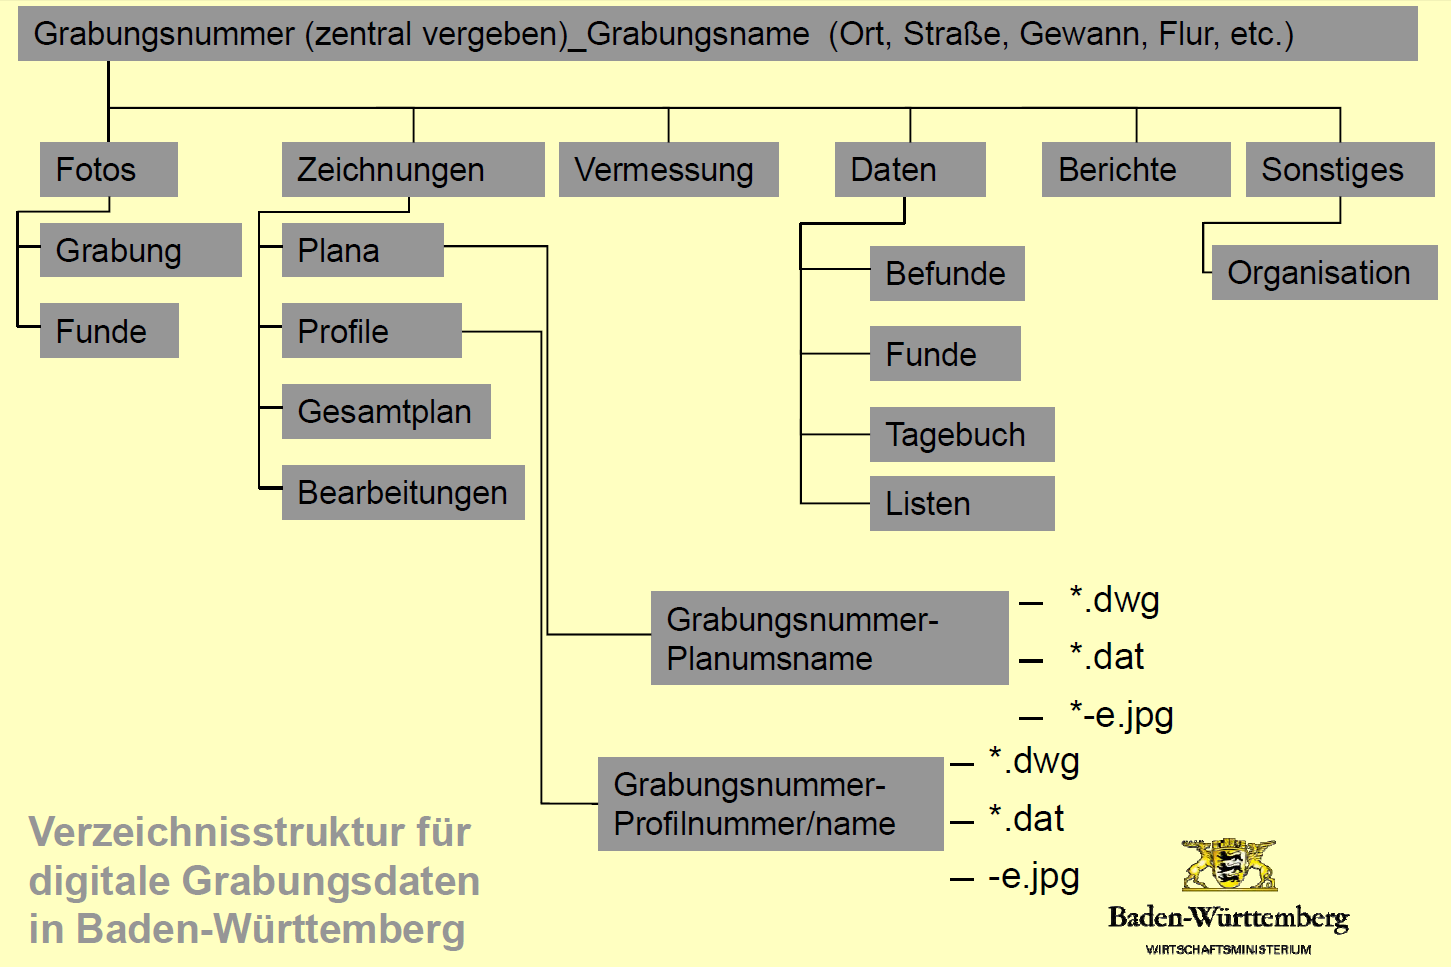
\includegraphics[width=0.9\textwidth]{bilder/OrdnerstrukturBaWue_Bibby}
  \end{center}
  \caption{Datenstruktur Baden-Württemberg}
  \label{OrdnerstrukturBaWue}
\end{figure}

"`\emph{Diese Struktur ist in den oberen Ebenen rigide genug, um für Ordnung und Datendisziplin zu sorgen und gleichzeitig weiter unten flexibel genug, um den unausweichlichen Eigenarten der einzelnen Archäologen Rechnung tragen zu können.}

\emph{Die Grabungs- oder Vorgangsnummer, die zentral vergeben wird, ist wichtig. Sie beschreibt nicht nur die Ausgrabung, sie ist auch die Inventar"=Stammnummer aller Funde, die auf dieser Grabung gefunden werden. Insofern ist sie die Schnittstelle zum zentralen Fundarchiv des Archäologischen Landesmuseums. Die Ausgräber werden aber nicht allein gelassen. Mit der Datenstruktur werden Anleitungen geliefert, die beschreiben, was wohin gehört. Damit wird tatsächlich eine gewisse Einheit im Land erreicht.}"'\footnote{D. Bibby, Digitale Datenstruktur auf Ausgrabungen und Archivierung digitaler Grabungsdaten. Praxis und Praxisversuche aus Baden-Württemberg, ANachr 14 2009, 159-163.}

Auch die nachträgliche Strukturierung von bereits vorhandenen digitalen Dateiablagen ist relativ einfach, da Klartextinhaltsverzeichnisse in der obersten Ebene des Verzeichnisses abgelegt werden können, welche die Eigenheiten der Grabung und die strukturellen Abweichungen beschreiben.

Der Aktenplan des Archäologischen Museums Hamburg wurde für ein analoges Projektarchiv entwickelt, lässt sich jedoch mit wenigen Anpassungen auch gut auf eine digitale Dateiablage anwenden. 

%HAMBURG
\begin{center}
	\begin{longtable}{l l l l}
		\toprule
		\multicolumn{2}{l}{Aktenplan des Archäologischen Museums Hamburg} \\ \midrule \endfirsthead
		\multicolumn{2}{l}{\footnotesize Fortsetzung der vorhergehenden Seite}\\
		\toprule
		\multicolumn{2}{l}{Aktenplan des Archäologischen Museums Hamburg}\\ \midrule \endhead
		\bottomrule \multicolumn{2}{r}{{\footnotesize Fortsetzung auf der nächsten Seite}} \\
		\endfoot
		\bottomrule 
		\endlastfoot
		
		\multicolumn{2}{l}{
\includegraphics[width=0.4cm]{bilder/OrdnerIconZu.png} \hspace*{0.04cm} Datenträger \textit{(nur analog)}}\\
		
		\multicolumn{2}{l}{
\includegraphics[width=0.4cm]{bilder/OrdnerIconAuf.png} \hspace*{0.04cm} Berichte}\\
		& 
\includegraphics[width=0.4cm]{bilder/DateiIcon.png}\hspace*{0.04cm} Grabungsbericht\\
		& 
\includegraphics[width=0.4cm]{bilder/DateiIcon.png} \hspace*{0.04cm} Zwischenberichte\\
		& 
\includegraphics[width=0.4cm]{bilder/DateiIcon.png} \hspace*{0.04cm} Anlagen Zwischenberichte\\
		
		\multicolumn{2}{l}{
\includegraphics[width=0.4cm]{bilder/OrdnerIconAuf.png} \hspace*{0.04cm} Vermessung}\\
	    & 
\includegraphics[width=0.4cm]{bilder/DateiIcon.png} \hspace*{0.04cm} Vermessungspläne\\
		& 
\includegraphics[width=0.4cm]{bilder/DateiIcon.png} \hspace*{0.04cm} Vermessungsunterlagen\\
		& 
\includegraphics[width=0.4cm]{bilder/DateiIcon.png} \hspace*{0.04cm} Vermessungsprotokolle\\
		
		\multicolumn{2}{l}{
\includegraphics[width=0.4cm]{bilder/OrdnerIconAuf.png} \hspace*{0.04cm} Grabungsplänge}\\
	    & 
\includegraphics[width=0.4cm]{bilder/DateiIcon.png} \hspace*{0.04cm} Zeichnungsliste\\
		& 
\includegraphics[width=0.4cm]{bilder/DateiIcon.png} \hspace*{0.04cm} Übersichtpläne\\
		& 
\includegraphics[width=0.4cm]{bilder/DateiIcon.png} \hspace*{0.04cm} Einzelpläne\\
		& 
\includegraphics[width=0.4cm]{bilder/DateiIcon.png} \hspace*{0.04cm} Arbeitspläne\\
		& 
\includegraphics[width=0.4cm]{bilder/DateiIcon.png} \hspace*{0.04cm} Handzeichnungen und Skizzen\\
		
		\multicolumn{2}{l}{
\includegraphics[width=0.4cm]{bilder/OrdnerIconAuf.png} \hspace*{0.04cm} Tagebuch}\\
	    & 
\includegraphics[width=0.4cm]{bilder/DateiIcon.png} \hspace*{0.04cm} Tagebuchausdruck \textit{(oder digitale Datei)}\\
		& 
\includegraphics[width=0.4cm]{bilder/DateiIcon.png} \hspace*{0.04cm} Notizen\\
		
		\multicolumn{2}{l}{
\includegraphics[width=0.4cm]{bilder/OrdnerIconAuf.png} \hspace*{0.04cm} Befunddokumentation}\\
	    & 
\includegraphics[width=0.4cm]{bilder/DateiIcon.png} \hspace*{0.04cm} Befundliste\\
		& 
\includegraphics[width=0.4cm]{bilder/DateiIcon.png} \hspace*{0.04cm} Befundkatalog\\
		& 
\includegraphics[width=0.4cm]{bilder/DateiIcon.png} \hspace*{0.04cm} Notizen\\
		
		\multicolumn{2}{l}{
\includegraphics[width=0.4cm]{bilder/OrdnerIconAuf.png} \hspace*{0.04cm} Funddokumentation}\\
	    & 
\includegraphics[width=0.4cm]{bilder/DateiIcon.png} \hspace*{0.04cm} Fundliste\\
		& 
\includegraphics[width=0.4cm]{bilder/DateiIcon.png} \hspace*{0.04cm} Inventarliste\\
		& 
\includegraphics[width=0.4cm]{bilder/DateiIcon.png} \hspace*{0.04cm} Schriftwechsel\\
		
		\multicolumn{2}{l}{
\includegraphics[width=0.4cm]{bilder/OrdnerIconAuf.png} \hspace*{0.04cm} Probendokumentation}\\
	    & 
\includegraphics[width=0.4cm]{bilder/DateiIcon.png} \hspace*{0.04cm} Probenliste\\
		& 
\includegraphics[width=0.4cm]{bilder/DateiIcon.png} \hspace*{0.04cm} Schriftwechsel\\
		
		\multicolumn{2}{l}{
\includegraphics[width=0.4cm]{bilder/OrdnerIconAuf.png} \hspace*{0.04cm} Fotodokumentation}\\
	    & 
\includegraphics[width=0.4cm]{bilder/DateiIcon.png} \hspace*{0.04cm} Fotoliste\\
		& 
\includegraphics[width=0.4cm]{bilder/DateiIcon.png} \hspace*{0.04cm} Miniaturausdruck \textit{(oder originale Dateien)}\\
		
		\multicolumn{2}{l}{
\includegraphics[width=0.4cm]{bilder/OrdnerIconAuf.png} \hspace*{0.04cm} Dokumente}\\
	    & 
\includegraphics[width=0.4cm]{bilder/DateiIcon.png} \hspace*{0.04cm} Pläne\\
		& 
\includegraphics[width=0.4cm]{bilder/DateiIcon.png} \hspace*{0.04cm} Dokumente und Texte\\
		& 
\includegraphics[width=0.4cm]{bilder/DateiIcon.png} \hspace*{0.04cm} Schriftwechsel\\
		& 
\includegraphics[width=0.4cm]{bilder/DateiIcon.png} \hspace*{0.04cm} Pressespiegel\\
		\bottomrule
	\end{longtable}
\end{center}

Das Bundesdenkmalamt in Österreich hat in seinen Richtlinien eine verpflichtende Ordnerstruktur veröffentlicht, die in einem übergeordneten Ordner mit der Kennung und Benennung der Maßnahme abgelegt wird. Bemerkenswert an dieser Ordnerstruktur ist die sehr flache Hierarchie ohne verschachtelte Ordner, die ein Hinzufügen weiterer benötigter Ordner in der gleichen Ebene zulässt. 

Für die Dateien 01-03 sind in den Richtlinien detaillierte Angaben über den erwarteten Inhalt zu finden. Dies gilt in etwas geringerem Umfang für die übrigen Ordner.  
%ÖSTERREICH
\begin{center}
	\begin{longtable}{l}
		\toprule
		Ordnerstruktur des Bundesdenkmalamtes Österreich \\ \midrule \endfirsthead
		\footnotesize Fortsetzung der vorhergehenden Seite\\
		\toprule
		Ordnerstruktur des Bundesdenkmalamtes Österreich \\ \midrule \endhead
		\bottomrule \multicolumn{1}{r}{{\footnotesize Fortsetzung auf der nächsten Seite}} \\
		\endfoot
		\bottomrule 
		\endlastfoot
		
		
\includegraphics[width=0.4cm]{bilder/DateiIcon.png} \hspace*{0.04cm} 01 Deckblatt\\
		\includegraphics[width=0.4cm]{bilder/DateiIcon.png} \hspace*{0.04cm} 02 Bericht -- Teil A\\
		\includegraphics[width=0.4cm]{bilder/DateiIcon.png} \hspace*{0.04cm} 03 Bericht -- Teil B\\
		\includegraphics[width=0.4cm]{bilder/OrdnerIconZu.png} \hspace*{0.04cm} 04 Technische Daten\\
		\includegraphics[width=0.4cm]{bilder/OrdnerIconZu.png} \hspace*{0.04cm} 05 SE-Liste \textit{(Liste der Stratigrafischen Einheiten)}\\
		\includegraphics[width=0.4cm]{bilder/OrdnerIconZu.png} \hspace*{0.04cm} 06 SE-Protokollblätter\\
		\includegraphics[width=0.4cm]{bilder/OrdnerIconZu.png} \hspace*{0.04cm} 07 Objektlisten\\
		\includegraphics[width=0.4cm]{bilder/OrdnerIconZu.png} \hspace*{0.04cm} 08 Objektgruppenlisten \emph{(fakultativ)}\\
		\includegraphics[width=0.4cm]{bilder/OrdnerIconZu.png} \hspace*{0.04cm} 09 Planliste\\
		\includegraphics[width=0.4cm]{bilder/OrdnerIconZu.png} \hspace*{0.04cm} 10 Fundliste\\
		\includegraphics[width=0.4cm]{bilder/OrdnerIconZu.png} \hspace*{0.04cm} 11 Grabungs- bzw. Prospektionsprotokoll\\
		\includegraphics[width=0.4cm]{bilder/OrdnerIconZu.png} \hspace*{0.04cm} 12 Vermessungsunterlagen\\
		\includegraphics[width=0.4cm]{bilder/OrdnerIconZu.png} \hspace*{0.04cm} 13 Originalmessdaten und/oder Metadaten Prospektion\\
		\includegraphics[width=0.4cm]{bilder/OrdnerIconZu.png} \hspace*{0.04cm} 14 Maßnahmenpolygon\\
		\includegraphics[width=0.4cm]{bilder/OrdnerIconZu.png} \hspace*{0.04cm} 15 Technischer Gesamtplan\\
		\includegraphics[width=0.4cm]{bilder/OrdnerIconZu.png} \hspace*{0.04cm} 16 Detailpläne\\
		\includegraphics[width=0.4cm]{bilder/OrdnerIconZu.png} \hspace*{0.04cm} 17 Fotodokumentation\\
		\includegraphics[width=0.4cm]{bilder/OrdnerIconZu.png} \hspace*{0.04cm} 18 Matrix\\
		\includegraphics[width=0.4cm]{bilder/OrdnerIconZu.png} \hspace*{0.04cm} 19 Konservatorische Maßnahmen\\
		\includegraphics[width=0.4cm]{bilder/OrdnerIconZu.png} \hspace*{0.04cm} 20 Sonstige Daten\\
		
		\bottomrule
	\end{longtable}
\end{center}


\hyphenation{
Schnitt-stel-le
}
\label{dateibenennung}
\subsection{Dateibenennung}
Üblicherweise besteht der Dateiname einer Datei aus dem eigentlichen Namen und der durch einen Punkt getrennten Dateinamenserweiterung, die das Format der Datei angibt. Die Erweiterung wird in der Regel von dem Programm, mit dem die Datei gespeichert wurde, automatisch an den Dateinamen gehängt.

Ein Beispiel: \emph{IT-Empfehlungen.pdf} gibt an, dass es sich um eine Datei mit dem Namen \emph{"`IT-Empfehlungen"'} handelt, die in dem PDF-Format vorliegt.

Da die Erweiterung automatisch erzeugt wird, muss die Datei mit einem geeigneten Programm konvertiert werden, wenn man das Dateiformat ändern möchte. In dem Kapitel "`Dateiformate"' ab Seite \pageref{dateiformate} sind ausführliche Informationen darüber zu finden.

Im Folgenden geht es nur noch um den reinen Dateinamen, ohne die Dateinamenserweiterung.

\subparagraph{Erlaubte Zeichen} Moderne Betriebssysteme können mit Sonderzeichen umgehen, zu denen Umlaute und Leerzeichen gehören. Das war aber nicht immer so und kann auch heute noch zu Problemen führen. Webserver lesen zum Beispiel das Leerzeichen als die Zeichenfolge "`$\%20$"' ein und da Umlaute nicht immer gleich kodiert werden, kann auch das zu Schwierigkeiten führen. 

Für die Langzeitarchivierung sollten also nur die alphanumerischen Zeichen des englischen Alphabets, also a-z, A-Z und 0-9 verwendet werden. Zusätzlich kann der Bindestrich ({\bfseries -}) und bei Bedarf auch der Unterstrich ({\bfseries\_}) verwendet werden.

\subparagraph{Zu vermeidende Zeichen} Es gibt eine ganze Reihe von Zeichen, die für besondere Aufgaben von Betriebssystemen verwendet werden. Der Punkt dient zur Trennung des Dateinamens von der Dateinamenserweiterung und der Schrägstrich dient in Windows um Ordnerebenen zu kennzeichnen.

Zu den Zeichen, die absolut nicht verwendet werden dürfen, gehören:
\begin{center}
	\Large \bfseries \textbackslash	 / : * ? "'	< >	|
\end{center}

Die Verwendung von allen weiteren Sonderzeichen ist zwar möglich, kann jedoch zu einem unerwarteten Verhalten des Systems führen. Daher wird von der Verwendung von Leerzeichen und Sonderzeichen, Bindestrich ({\bfseries -}) und Unterstrich ({\bfseries\_}) ausgenommen, abgeraten.

\subparagraph{Groß- und Kleinschreibung} Die Groß- und Kleinschreibung in einem Dateinamen wird von unterschiedlichen Systemen verschieden gedeutet. In Windows beispielsweise kann, wenn es eine Datei mit dem Namen \emph{"`TestDatei"'} schon gibt, keine Datei mit dem Namen \emph{"`testdatei"'} angelegt werden. Andere Systeme könnten dies jedoch erlauben, was aber nicht bedeutet, dass man dies auch tun sollte.

Hat man sich in der Praxis einmal für eine Schreibweise entschieden, muss diese auch konsequent eingehalten werden und insbesondere bei der Arbeit auf verschiedenen Systemen darauf geachtet werden.

\subparagraph{Länge} Der Dateiname sollte so kurz wie möglich und so lang wie nötig sein. Eine aktuelle Obergrenze, die auf manchen Systemen nicht überschritten werden darf, sind 260 Zeichen, wobei dabei der gesamte Dateipfad gezählt wird. Kryptische oder untypische Kürzel sollten vermieden werden, da sie in der Regel in Vergessenheit geraten.

\subsection{Versionskontrolle}\label{versionskontrolle}
Wenn unterschiedliche Personen an einer Datei arbeiten, ist es wichtig, die verschiedenen Änderungen und Entwicklungsstadien zu verfolgen und zu kennzeichnen. Nur so kann vermieden werden, dass an der falschen Dateiversion gearbeitet wird oder diese gar gelöscht wird. Dateiversionen, die nicht mehr benötigt werden, sollten bei Bedarf gelöscht werden.

Es gibt mehrere Strategien, um die Versionskontrolle durchzuführen, die im Folgenden erläutert werden.

\subparagraph{Angabe im Dateinamen} Eine einfache und übersichtliche Methode ist, die Versionsangabe in den Dateinamen zu integrieren. Das kann beispielsweise mit einer Datumsangabe oder Ziffern erfolgen. Durch ein vorangestelltes {\bfseries v} werden die Ziffern als eine Versionsnummer gekennzeichnet, wie zum Beispiel {\bfseries v001}. Führende Nullen stellen sicher, dass die Versionsnummern einheitlich und leichter lesbar sind und richtig sortiert werden.

Eine Kennzeichnung von Versionen durch Worte wie \emph{"`neu"'}, \emph{"`neuer"'} und \emph{"`alt"'} ist unbedingt zu vermeiden. Eine Ausnahme können endgültige Dateiversionen bilden, die der Übersicht halber etwa durch \emph{FINAL} am Ende gekennzeichnet werden können. Es darf aber nur eine Datei mit dieser Kennzeichnung in einem Ordner und einem bestimmten Format vorliegen. Eine endgültige Version, die zum Beispiel sowohl als \emph{docx} als auch als \emph{pdf} vorliegt, ist also erlaubt.

\subparagraph{Angabe in der Datei} Angaben zum Erstellungsdatum und den verschiedenen Versionen und deren Änderungen können im Header der Datei oder in standardisierten Kopfzeilen in der Datei selbst angegeben werden. Bei Textdokumenten bietet sich die Möglichkeit einen Innentitel mit einer Versionshistorie zu verwenden. Ein Beispiel für solch einen Innentitel findet sich am Anfang der PDF-Version dieser Empfehlungen.

\subparagraph{Änderungsprotokoll} Statt einzelne Dateiversionen abzuspeichern, kann auch ein Änderungsprotokoll geführt werden. Dabei werden die einzelnen Änderungen in einer einfachen Textdatei protokolliert, die zusammen mit der eigentlichen Datei abgelegt wird. Im Englischen wird dafür der Begriff \emph{ChangeLog} verwendet.

\subparagraph{Software} Die bisher beschriebenen Methoden sind hauptsächlich manuell anzuwendende Vorgänge. Es gibt jedoch auch Software zur Versionsverwaltung. Deren Einsatz lohnt sich vor allem in großen Projekten, die zentral auf einem Server abgelegt werden. Versionsverwaltungssoftware kann aus den Dateiänderungen automatisch \emph{ChangeLogs} erstellen. Die am weitesten verbreiteten Systeme zur Versionsverwaltung sind \href{http://subversion.apache.org/}{Subversion (SVN)} und \href{https://git-scm.com/}{Git}. Primär wurden sie für die Bedürfnisse von Softwareentwicklern konzipiert, jedoch eignen sie sich auch für allgemeinere Aufgaben. Für die einzelnen Computerarbeitsplätze werden Clients wie \href{https://tortoisesvn.net/}{TortoiseSVN} für SVN oder \href{https://windows.github.com/}{GitHub} für Git benötigt.

Eine einfache Versionsverwaltung für Dateien bieten \href{https://owncloud.org/}{ownCloud}, \href{https://www.dropbox.com/}{Dropbox} und \href{https://drive.google.com/drive/}{Google Drive} wobei die Menge der unterschiedlichen gespeicherten Versionen abhängig von dem persönlichen Speicherplatz ist.

\begin{flushleft}
Git: \urllist{https://git-scm.com/}
Clients für Git: \urllist{https://git-scm.com/downloads/guis}
Subversion (SVN): \urllist{http://subversion.apache.org/}
TortoiseSVN: \urllist{https://tortoisesvn.net/}
ownCloud: \urllist{https://owncloud.org/}
Dropbox: \urllist{https://www.dropbox.com/}
Google Drive: \urllist{https://drive.google.com/drive/}
Vergleich von Versionsverwaltungssystemen auf Wikipedia: \urllist{https://en.wikipedia.org/wiki/Comparison_of_revision_control_software}
\end{flushleft}

\newpage
\section{Dateispeicherung und -sicherung}\label{dateispeicherung}
\abschnittsautor{M. Trognitz, R. Komp, R. Förtsch}
Um Datenverlust vorzubeugen, ist es unerlässlich eine geeignete Sicherungsstrategie zu verwenden. Dabei muss zwischen einer kurzfristigen Speicherung und einer mittelfristigen Sicherung unterschieden werden. Ersteres meint, wie Daten während der Erstellung und Bearbeitung gespeichert werden. Letzteres bezieht sich auf einen längeren Speicherzeitraum, der durchaus auch mehrere Monate betragen kann, stellt also ein klassisches Backup der Daten dar.

Die Sicherungsstrategie legt fest, wie die Datensicherung erfolgen soll und berücksichtigt folgende Fragen:
\begin{itemize}
	\item Wer ist für die Datensicherung verantwortlich?
	\item Wer hat Zugriff auf die gesicherten Daten?
	\item Wann und wie oft soll die Datensicherung durchgeführt werden?
	\item Auf welche Weise soll gesichert werden?
	\item Welche Daten sollen gesichert werden?
	\item Welche Speichermedien sollen verwendet werden?
	\item Wie viele Sicherungskopien sollen angelegt werden?
	\item Wo sollen die Sicherungen aufbewahrt und wie sollen sie geschützt werden?
	\item Wie soll der Transport der Sicherungskopien erfolgen?
	\item Wie lange soll eine Sicherung aufbewahrt werden?
\end{itemize}

Die Sicherungsstrategie kann mit den zu verwendenden Richtlinien zur Dateiablage eng verzahnt sein, um etwa einen nahezu automatisierten Sicherungsvorgang zu ermöglichen.

Die richtige Speicherstrategie beugt zwar möglichen Datenverlusten durch Hardware-, Software- oder menschliche Fehler vor, stellt aber noch \emph{keine} Archivierung der Daten dar. Eine Archivierung ist auf Langfristigkeit ausgelegt und impliziert immer eine bewusste Auswahl und umfassende Dokumentation der Daten, da eine Nachnutzung derselben das Ziel ist. Während der Projektlaufzeit kann bereits ein eigener Archivordner angelegt werden, worin beispielsweise finale Dateien oder unprozessierte Rohdaten abgelegt werden können, um die spätere Auswahl der zu archivierenden Daten vorzubereiten und zu vereinfachen.

Weiterführende Hinweise zur Datensicherung sind auf den Seiten des Bundesamtes für Sicherheit in der Informationstechnik zu finden, die sich sowohl an Einsteiger\footnote{\url{https://www.bsi-fuer-buerger.de/BSIFB/DE/MeinPC/Datensicherung/Sicherungsmethoden/sicherungsmethoden\_node.html}} als auch an Experten\footnote{\url{https://www.bsi.bund.de/DE/Themen/ITGrundschutz/ITGrundschutzKataloge/Inhalt/\_content/baust/b01/b01004.html}} richten. 
\subsection{Kurzfristige Speicherung}
Zur Bearbeitung geöffnete Dateien sollten in kürzeren Abständen gespeichert werden, um einem Verlust von stundenlanger Arbeit infolge etwa eines Stromausfalls vorzubeugen. Von diesen Arbeitsversionen sollten regelmäßig, beispielsweise nach jedem Arbeitstag, Kopien auf externen Speichermedien angefertigt werden, welche in die mittelfristige Sicherung übergehen.

Vorgaben zur Form der Dateiablage, der Dateibenennung und Versionierung müssen schon beim Anlegen der Dateien beachtet werden, um einen reibungslosen Ablauf der darauf abgestimmten Datensicherungsstrategie zu gewährleisten. Hinweise dazu sind im Abschnitt Dateiverwaltung ab Seite \pageref{dateiverwaltung} zu finden.

\subsection{Mittelfristige Sicherung}
Digitale Daten sind nur dann über einen längeren Zeitraum sicher, wenn sie mehr als einmal gespeichert werden. Es müssen also mindestens zwei Sicherungskopien auf physisch getrennten Speichermedien vorliegen, um etwa bei einem Hardwaredefekt auf eine alternative Sicherungskopie zugreifen zu können.

Die Sicherung von Daten auf unterschiedlichen Arbeitsgeräten wird erleichtert, wenn diese zunächst auf einem Datenträger gesammelt werden und dieser dann gesichert wird.

\subparagraph{Speichermedium} Welches Speichermedium gewählt wird, hängt vor allem von der Speichergröße der zu sichernden Dateien und der vorhandenen Infrastruktur ab. So eignen sich eine CD oder eine DVD nur für Daten bis maximal 900 MB bzw. 17 GB Speichervolumen. Für größere Datenmengen werden entsprechend größere Datenträger benötigt. 

Steht ein lokaler oder institutioneller Server zur Verfügung, sollte dieser zur Datensicherung verwendet werden, da diese üblicherweise gewartet werden und meist selbst in eigene Sicherungsstrategien eingebunden sind. In Umgebungen mit Zugriff auf das Internet, kann eine Sicherung auch auf einen entfernten Server, beispielsweise in einem Rechenzentrum, erfolgen. In allen anderen Fällen können externe Festplatten verwendet werden. Von externen kommerziellen Diensten, wie beispielsweise Dropbox, ist für eine mittelfristige Sicherung abzuraten, weil es sich oft um ausländische Anbieter handelt, die nicht dem deutschen Recht unterliegen und den Nutzer im Unklaren darüber lassen, wie mit den Daten umgegangen wird.

Da die Speichermedien eine begrenzte Lebenszeit von etwa zehn Jahren haben, sollten die Sicherungen von Zeit zu Zeit auf neue Speichermedien migriert werden. Außerdem sollten sie zwischenzeitlich an verschiedenen Orten, mindestens in verschiedenen Räumen, gelagert werden, um etwa im Brandfall den Schaden zu begrenzen. Auch der Transport von Original- und Sicherungsdatenbeständen sollte getrennt durch unterschiedliche Personen erfolgen, um zu vermeiden, dass etwa durch Diebstahl alle Sicherungskopien auf einmal abhanden kommen. 

Für das Kopieren der Daten auf ein Speichermedium gibt es verschiedene Methoden, wie die im Folgenden beschriebene Volldatensicherung, inkrementelle und differentielle Datensicherung.

\subparagraph{Volldatensicherung} Bei der Volldatensicherung werden die zu sichernden Dateien komplett und eins zu eins auf ein Speichermedium kopiert. Wird zum ersten Mal eine Sicherungskopie angelegt, so muss dies als Volldatensicherung geschehen. Dabei ist zu beachten, dass der Kopiervorgang viel Zeit in Anspruch nehmen kann, wobei dies auch über Nacht geschehen kann. Vor der Ausführung der Volldatensicherung muss geprüft werden, dass auf dem Speichermedium ausreichend freier Speicherplatz vorhanden ist. 

Die Volldatensicherung ist die einzige Methode, die manuell, ohne weitere Hilfsprogramme, durchgeführt werden kann. Wird eine Volldatensicherung angelegt, sollten, beispielsweise in einer Textdatei, Informationen gespeichert werden, die Auskunft über den Zeitpunkt der Sicherung, den Ansprechpartner und den Umfang der Daten geben.

Liegt eine erste Volldatensicherung vor, können neue oder geänderte Daten mittels inkrementeller oder differentieller Datensicherung gesichert werden, was die Möglichkeit bietet, verschiedene Versionen der Daten zu sichern. Für beide Methoden werden jedoch eigene Programme benötigt.

\subparagraph{Inkrementelle Sicherung} Die inkrementelle Sicherung speichert nur jene Daten, die sich im Vergleich zu der vorliegenden Volldatensicherung oder vergangenen inkrementellen Sicherungsvorgängen geändert haben. Dies spart Zeit und Speicherplatz, erfordert jedoch im Fall einer Wiederherstellung der Daten, dass zunächst die Volldatensicherung übertragen wird und anschließend alle erfolgten inkrementellen Sicherungen nacheinander eingespielt werden.

\subparagraph{Differentielle Sicherung} Bei der differentiellen Sicherung werden immer jene Daten gespeichert, die sich im Verlgeich zu der vorliegenden letzten Volldatensicherung geändert haben. Im Unterschied zu der inkrementellen Sicherung entfällt also der Vergleich mit Daten aus zwischenliegenden Sicherungsvorgängen seit Erstellung der Volldatensicherung. Diese Methode erfordert zwar etwas mehr Zeit und Speicherplatz als die inkrementelle Sicherung, erleichtert aber die Wiederherstellung der Daten, da nur die Volldatensicherung und die letzte differentielle Sicherung auf das System übertragen werden muss. Die vorherigen differentiellen Sicherungen werden nicht benötigt.

\subparagraph{Automatisierung} Die Datensicherung kann mit Hilfe von Programmen oder Skripten automatisiert erfolgen. Wichtig ist dabei zu kontrollieren, dass die Datensicherung auch tätsächlich in der gewünschten Form ausgeführt wird. Geeignete Programme gibt es viele, wie beispielsweise \href{http://bacula.org/}{Bacula}, \href{http://www.dirsyncpro.org/}{DirSync Pro}, \href{http://www.traybackup.de}{TrayBackup}, \href{http://personal-backup.rathlev-home.de}{PersonalBackup} oder \href{http://rsync.samba.org/}{rsync}. Eine ausführliche Liste ist außerdem auf der englischen Wikipedia unter \href{http://en.wikipedia.org/wiki/List\_of\_backup\_software}{List of backup software} zu finden. Oft können die Programme auch zur Wiederherstellung von gesicherten Daten verwendet werden.

\begin{flushleft}
	DirSync Pro: \urllist{http://www.dirsyncpro.org/}
	TrayBackup: \urllist{http://www.traybackup.de}
	PersonalBackup: \urllist{http://personal-backup.rathlev-home.de}
	rsync: \urllist{http://rsync.samba.org/}
	Liste von Backup-Programmen auf Wikipedia: \urllist{http://en.wikipedia.org/wiki/List_of_backup_software} 
\end{flushleft}

\subparagraph{Sicherungszeitpunkt} Der Zeitpunkt der Sicherung spielt eine nicht zu unterschätzende Rolle. Beispielsweise kann eine Sicherung von Datenbanken im laufenden Betrieb zu Inkonsistenzen führen, weshalb in solchen Fällen ein Administrator diese Aufgabe übernehmen sollte.

Regelmäßige Sicherungsvorgänge, die zu bestimmten Zeitpunkten täglich, wöchentlich oder monatlich automatisiert gestartet und durchlaufen werden, gewährleisten, dass eine Sicherung auch tatsächlich erfolgt, zumal sie nicht vom individuellen Verhalten eines Nutzers abhängen.

Für Daten, die verschiedene Arbeitsschritte durchlaufen und dadurch große Änderungen erfahren, können die verschiedenen Zustände als Sicherungspunkte gespeichert werden. Beispielsweise können zunächst unbearbeitete digitale Bilder gespeichert werden, sowie ein daraus erzeugtes photogrammetrisches Modell oder andere nicht oder nur schwer reproduzierbare signifikante Verarbeitungsschritte. Solche Sicherungspunkte müssen allerdings manuell gemacht werden, indem beispielsweise ein Ordner mit den Rohdaten angelegt wird. Hinweise für solche Sicherungspunkte werden für bestimmte angewendete Methoden in dem Kapitel Forschungsmethoden ab Seite \pageref{methoden} gegeben.

\subparagraph{Sicherungsversionen} Es empfiehlt sich, eine vorhandene Volldatensicherung nicht direkt mit einer neuen Volldatensicherung zu überschreiben. Tritt nämlich während des Sicherungsvorganges ein Fehler auf, könnte auch die bereits vorhandene Sicherungsversion beschädigt werden.

Bei der Anwendung von inkrementellen oder differentiellen Sicherungsmethoden sollte trotzdem in geregelten Zeitabständen eine neue Volldatensicherung angelegt werden, welche mindestens bis zur nächsten Volldatensicherung aufgehoben wird. Dies ist im Sinne des Generationenprinzips oder Großvater-Vater-Sohn-Prinzips, einer Strategie zur Datensicherung, bei der mehrere Sicherungen für verschiedenen Zeitpunkte und Zwecke angelegt werden. Hierfür können beispielsweise wöchentlich und monatlich Volldatensicherungen angelegt werden (Vater und Großvater), die primär den Datenverlust durch Hardware- oder Software-Fehler reduzieren sollen. Tägliche inkrementelle oder differentielle Sicherungen (Sohn) erlauben es beispielsweise auf Arbeitsversionen des Vortages zuzugreifen und können mit dem Beginn einer neuen Woche nach und nach überschrieben werden. 

\subparagraph{Disaster Recovery} Eine gute Sicherungsstrategie umfasst zusätzlich die Erprobung der Wiederherstellung der Daten, um im Ernstfall sicher zu sein, dass die verwendete Strategie auch wirklich funktioniert und die Daten schnell wieder einsatzfähig sind. Somit können vorhandene Sicherungsversionen ebenfalls auf ihre Funktionsfähigkeit überprüft werden.
	
%Dateiformate
	\chapter{Dateiformate}
	\abschnittsautor{F. Schäfer}
	\label{dateiformate}
Im Folgenden werden konkrete technische Hinweise und Hintergrundinformationen zu den Dateiformaten gegeben, die nach heutigem Wissen für die Langzeitarchivierung geeignet sind. Des Weiteren werden die minimalen Anforderungen an die technische wie inhaltliche Dokumentation von einzelnen Dateiformaten genannt, damit diese nicht nur heute, sondern auch in Zukunft von Dritten verstanden und nachgenutzt werden können.

Es geht hier nur um die Dateiformate an sich, ihre Entstehungsweise wird dabei nicht berücksichtigt. Abhängig von der jeweiligen Generierung und Verwendung sind gegebenfalls zusätzliche methodische und fachspezifische Metadaten erforderlich. Diese werden in dem Kapitel Forschungsmethoden ab Seite \pageref{methoden} beschrieben.

Bereits die Auswahl der verwendeten Software beeinflusst das Dateiformat und dessen Nachhaltigkeit. Daher sollte bei der Entscheidung für oder gegen eine bestimmte Software darauf geachtet werden, dass Dateiformate unterstützt werden, die möglichst folgende Eigenschaften aufweisen:
\begin{itemize}
	\item Weit verbreitet und standardisiert
	\item Nicht proprietär, also nicht von einer Anwendung oder einem Hersteller abhängig und mit unterschiedlichen Programmen verwendbar
	\item Offen dokumentiert mit frei verfügbaren technischen Spezifikationen
	\item Verlustfreie oder keine Kompression
	\item Einfach dekodierbar oder sogar unmittelbar lesbar, also nicht durch Kodierung versteckt
\end{itemize} 

Werden während eines Arbeitsprozesses andere als die hier empfohlenen Dateiformate erzeugt oder verwendet, sollte darauf geachtet werden, dass diese leicht und mit möglichst geringem Verlust an Informationen und Funktion in eines der in den folgenden Kapiteln aufgeführten Langzeitformate überführt werden können. 

In den Übersichtstabellen mit den Formaten für bestimmte Dateitypen sind die präferierten Formate mit einem grünen Haken, die noch akzeptablen mit einer gelben Tilde und für die Langzeitarchivierung ungeeignete Formate mit einem roten Kreuz gekennzeichnet.

\newpage
\section{PDF-Dokumente}
\label{pdf-dokumente}
\abschnittsautor{S. Jahn; Mit Unterstützung von: D. von Seggern}
	Das PDF (Portable Document Format) wurde 1993 von Adobe Systems entwickelt, um den Datenaustausch zu erleichtern. Es ist ein plattformunabhängiges, offenes Dateiformat, das 2008 mit der Version 1.7 als ISO-Standard zertifiziert wurde und seitdem von der ISO weiter gepflegt wird.  

Der große Vorteil von PDFs liegt darin, dass Dateiinhalte unabhängig vom Betriebssystem, dem ursprünglichen Anwendungsprogramm und der Hardwareplattform unverändert dargestellt werden. Das Aussehen von Dokumenten wird, wie bei einem analogen Ausdruck, eingefroren und kann somit angezeigt werden, wie es ursprünglich vom Autor intendiert war.  Gleichzeitig sind die Möglichkeiten zur nachträglichen Bearbeitung begrenzt, wodurch eine große Authentizität gewährleistet wird.

Für das Öffnen einer PDF-Datei gibt es verschiedene freie Anwendungen, worin ein Grund für die große Verbreitung und Akzeptanz von PDFs liegt. Viele Programme können Dateien direkt im PDF-Format speichern oder exportieren. Darüber hinaus lassen sich mit Hilfe von zusätzlich installierten Druckertreibern PDF-Dateien aus allen Programmen heraus erzeugen.

\subparagraph{Langzeitformate} Nicht jede Datei mit der Dateierweiterung .pdf  ist gleichermaßen für die Langzeitarchivierung geeignet. Für diesen Zweck  wurde das PDF/A-Format entwickelt und als ISO-Standard zertifiziert. Es beschreibt in welcher Form bestimmte Elemente in einer PDF-Datei enthalten sein müssen und welche nicht erlaubt sind. Die erste Version der PDF/A-Norm wurde nachträglich um zwei weitere, aufeinander aufbauende Normteile ergänzt. Wird das PDF/A-Format für die Langzeitarchivierung einer Datei verwendet, die nicht nur textuelle Informationen enthält, sollten nach Möglichkeit auch die ursprünglichen Ausgangsdateien in archivierungstauglichen Formaten entweder als separate Dateien oder integriert in das Container-Format PDF/A-3 mitarchiviert werden.

\begin{center}
	\begin{tabular}{l p{0.2\textwidth} p{0.6\textwidth}}
		\toprule
		\multicolumn{2}{l}{Format} & Begründung \\ \midrule
		\multirow{3}{*}{\color{ForestGreen} \LARGE \checkmark} & PDF/A-1 & \multirow{2}{*}{\parbox{0.6\textwidth}{PDF/A ist gezielt als stabiles, offenes und standardisiertes Format für die Langzeitarchivierung unterschiedlicher Ausgangsdateien entwickelt worden.}}\\
		& PDF/A-2 & \\
		& &\\
		\cmidrule(r){1-3}
		\multirow{1}{*}{$\color{BurntOrange} \thicksim$} & PDF/A-3 & PDF/A-3 ist nur dann für die Langzeitarchivierung geeignet, wenn alle eingebetteten Dateien in einem anerkannten Archivformat vorliegen.\\
		\cmidrule(r){1-3}
		\multirow{1}{*}{\LARGE \boldmath$\color{BrickRed} \times$}& andere PDF-Varianten & Viele gängige PDF-Varianten sind nicht für die Langzeitarchivierung geeignet. Stattdessen sollten entweder die Ausgangsdateien in einem passenden Format archiviert oder eine Migration in ein PDF/A-Format vorgenommen werden.\\
		\bottomrule
		\bottomrule
	\end{tabular}
\end{center}

\newpage
\subparagraph{Dokumentation}
Welche Metadaten für ein PDF-Dokument relevant sind, hängt von dessen Inhalt ab. Bei PDF-Dateien, die nur Text enthalten, sind meist weniger Informationen erforderlich, als bei PDFs, die Bilder, GIS-Karten oder 3D-Modelle enthalten. Die Metadaten können unmittelbar in einem PDF-Dokument im XMP-Format gespeichert werden.

Die hier angegebenen Metadaten sind als minimale Angabe zu betrachten und ergänzen die angegebenen Metadaten für Projekte und Einzeldateien in dem Abschnitt Metadaten in der Anwendung ab Seite \pageref{Metadaten-anwendung}.

\begin{center}
	\begin{tabular}{l p{0.6\textwidth}}
		\toprule
		Metadatum & Beschreibung \\ \midrule
Titel & Titel des Dokuments, nicht der Dateiname\\
Autor & Name des Verfassers oder Erstellers der Datei; gegebenfalls Name der Einrichtung\\
Stichwörter & Schlagworte, wie z.B. Periode, Fundstelle oder charakteristische Merkmale. Wenn vorhanden, angemessene Thesauri verwenden\\
Beziehungen & Dateien oder Ressourcen, die mit dem PDF zusammenhängen, insbesondere der Name der Originaldatei, aus der heraus ein PDF erstellt wurde\\
Anwendung & Programm, mit dem der Inhalt ursprünglich erzeugt wurde\\
Datum & Datum der Erstellung oder letzten Änderung der Datei\\
Copyright-Angaben & Angaben zur Person oder Einrichtung, die das Copyright oder die Lizenzrechte an der Datei oder deren Inhalt besitzt\\
\multicolumn{2}{l}{Zusätzliche Metadaten}\\
Kurzbeschreibung & Kurzbeschreibung über den Inhalt des Dokuments\\
Sprache & Sofern schriftliche Inhalte vorhanden sind, die Sprache angeben. Sprachkennungen nach ISO 639 angeben.\\
Verfasser der Metadaten & Name der Person, welche die Metadaten ausgefüllt hat\\
 		\bottomrule
		\bottomrule
	\end{tabular}
\end{center}

Weitere Metadaten sind abhängig vom Inhalt und der Methoden und können in den jeweiligen Abschnitten im Kapitel Forschungsmethoden ab Seite \pageref{methoden} nachgelesen werden.
	%Übersicht ist in getrennter Datei pdf-dokumente-uebersicht.
\paragraph{Vertiefung}
Eine wesentliche Eigenschaft und Stärke von PDF-Dateien ist, dass sie ganz unterschiedliche Inhalte enthalten können. So lassen sich neben Texten und Navigationshilfen, wie etwa Inhaltsverzeichnisse mit Textankern, auch andere Informationen wie Bilder, Verktorgrafiken, 3D-Visualisierungen, Tabellen, Präsentationen oder GIS-Karten einbinden, die zusammen mit allen ursprünglich verwendeten Layoutmerkmalen gespeichert werden. Daher werden die meisten Publikationen wie elektronische Zeitschriften oder Informationsmaterialien auf Webseiten üblicherweise als PDF-Dateien zur Verfügung gestellt. Bei der Langzeitarchivierung von Dateien spielt das PDF/A-Format eine besondere Rolle. In dessen Spezifikation wird unter anderem vorgeschrieben, Schriften in das Dokument einzubetten und Farben geräteneutral zu definieren. Auf diese Weise wird gewährleistet, dass das originale Aussehen eines Dokuments wie in der ursprünglichen Anwendung und wie vom Autor intendiert erhalten bleibt. Die Intention von PDF-Dateien ist insofern die Erhaltung der ursprünglichen Darstellung, nicht aber der ursprünglichen Bearbeitungsfunktionalitäten.

Um eine möglichst große Authentizität einer PDF-Datei zu erlangen, sind die Möglichkeiten zur nachträglichen Bearbeitung sehr begrenzt. Es können Kommentare hinzugefügt, Seiten eingebunden oder gelöscht, oder Textstellen geschwärzt werden. Eingeschränkt sind Veränderungen der eigentlichen Inhalte oder des Layouts möglich, wie z. B. Änderungen von Farben in einem Foto oder Umformulierungen von Texten. Als Nachteil ergibt sich daraus, dass die ursprüngliche Funktionalität der nach PDF/A konvertierten Datei verloren geht und eine Nachnutzung der Inhalte wenn überhaupt nur mit Qualitätsverlusten möglich ist. So können beispielsweise tabellarische Daten aus einer PDF-Datei nicht ohne einen zusätzlichen Mehraufwand in eine neue Tabelle übernommen werden, wobei Bearbeitungsfehler auftreten können.

Da aber zunehmend Softwarelösungen existieren, die diese Einschränkungen der nachträglichen Bearbeitung auflösen oder umgehen, wächst der Bedarf an Schutzmechanismen gegen ungewollte Änderungen durch Dritte. Dazu zählen beispielsweise die Festlegung von einfachen Nutzungseinschränkungen, wie etwa die Erlaubnis zum Drucken, zum Kopieren von Inhalten oder zur Bearbeitung der im PDF gespeicherten Metadaten, oder die Vergabe von Passwörtern. Für Dateien, bei denen eine Langzeitarchivierung vorgesehen ist, dürfen allerdings keine Schutzfunktionen verwendet werden, damit sie ohne Hindernisse jederzeit nutzbar sind. Falls notwendig können Einschränkungen als Lizenzhinweise formuliert werden; die Authentizität eines Dokumentes kann durch Signaturen, Zeitstempel und/oder digitale Prüfsummen gewährleistet werden.

\subparagraph{Inhalte}
Dateien im PDF-Format können durch unterschiedliche Anwendungen erzeugt werden und daher ganz unterschiedliche Inhalte enthalten und darstellen. Für jede Dateiart gibt es spezifische Aspekte, die es zu beachten gilt, insbesondere dass einige Inhalte nicht mit den Vorgaben von PDF/A vereinbar sind.

{\bfseries Texte:} Standardmäßig sind in PDF-Readern bereits 14 Schriftarten verfügbar. Es lassen sich aber auch weitere in ein PDF-Dokument einbetten, um eine korrekte Darstellung zu gewährleisten. Mithilfe von OCR-Software kann in PDF-Dokumenten eine nachträgliche Texterkennung durchgeführt werden.

{\bfseries Bilder:} Wie bei normalen Rastergrafiken können auch in PDF-Dateien eingebettete Bilder durch spezielle Kompressionsverfahren in ihrer Speichergröße reduziert und in ihrer Auflösung heruntergerechnet werden. Bei fast allen Verfahren ist dies mit einem Informationsverlust verbunden, der vor allem die Genauigkeit und Qualität der Anzeige betrifft.

{\bfseries Vektorgrafiken:} Vektorgrafiken in PDF-Dateien können wie die Ausgangsdateien frei skaliert werden.

{\bfseries 3D:} Es gibt zwei PDF-Formate, in die 3D-Dateien eingebettet und mit Adobe Reader geöffnet und betrachtet werden können. Auf diese Weise lassen sich auch 3D-Objekte austauschen und mit einfachen Funktionen bedienen, z. B. in der Ansicht drehen, Lichteinstellungen verändern oder Aufsichten und Schnittflächen erzeugen.

\subparagraph{PDF-Varianten}
PDF-Dateien sind inzwischen ein sehr weit verbreitetes Austauschformat, das in ganz unterschiedlichen Kontexten Verwendung findet. Um eine gleichbleibende Qualität zu gewährleisten, wurden für die häufigsten Anwendungsfälle mehrere Normen und Standards festgelegt:
\begin{itemize}
	\item PDF/X -- Format für die Übermittlung von Druckvorlagen (seit 2001)
	\item PDF/A -- Format für die elektronische Archivierung  (ISO 19005-1 seit 2005)
	\item PDF/E  -- Format für technische Dokumente aus den Bereichen Ingenieurwesen, Architektur und Geo"=Informationssysteme. Dieses Format besitzt die Fähigkeit zur interaktiven Darstellung von 3D-Objekten. Einzelteile können gedreht, auseinandergezogen, ein- oder ausgeblendet werden (ISO 24517 seit 2008)
	\item PDF/UA -- Richtlinien zum Aufbau eines barrierefreien Dokuments im Format PDF (seit 2008)
	\item PDF/VT  -- Format für den Einsatz im hochvolumigen und Transaktionsdruck (seit 2010)
\end{itemize}

Mehrere PDF-Standards lassen sich miteinander verbinden. Genügt eine Datei dem PDF/X-Standard, eignet sie sich als digitale Druckunterlage. Erfüllt diese Datei zusätzlich den PDF/UA-Standard, kann sie als barrierefreies PDF von Screenreader-Programmen verarbeitet werden. 

\subparagraph{Das Archivierungsformat PDF/A}
Von den verschiedenen existierenden PDF-Formaten ist nur das PDF/A-Format ein sicheres und stabiles Archivformat, das speziell für die elektronische Langzeitarchivierung von Dokumenten definiert und publiziert wurde. Die klar festgelegten und als Standard allgemein anerkannten Regeln schreiben vor, welche Bestandteile in einer PDF-Datei enthalten sein müssen und welche nicht zulässig sind, um mit dem PDF/A-Standard konform zu gehen. Während einige Inhaltstypen wie Texte, Bilder, Zeichnungen, Tabellen und Schriften standardkonform in PDF/A-Dateien eingebunden werden können, sind andere Inhalte wie 3D-Objekte, Audio- und Video-Sequenzen, Flash-Animationen oder Scripte nicht erlaubt. Ebenso darf eine PDF/A-Datei keine externen oder dynamischen Inhalte enthalten, die in einem Viewer geladen werden müssen. Beispielsweise werden URL-Links nur als Zeichenkette, nicht aber als aktive Verknüpfung gespeichert. Enthält eine PDF-Datei nicht zulässige Inhalte, kann sie nicht nach PDF/A konvertiert werden. Eine Validierung, ob eine vorliegende Datei dem gültigen PDF/A-Format entspricht, ist über entsprechende Prüfwerkzeuge möglich und wird im Praxisteil auf Seite \pageref{pdf-validierung} beschrieben.

Insgesamt sind aktuell drei, aufeinander aufbauende Versionen von PDF/A-Formaten zu unterscheiden, von denen PDF/A-1 und PDF/A-2 echte Archivformate sind, da sie das Dokument in einem stabilen Zustand konservieren. Bei PDF/A-3 handelt es sich hingegen um einen Container, in den beliebige Dateiformate eingebettet werden können. Der große Vorteil liegt also darin, dass editierbare Originaldateien in das Dokument integriert werden können. Es gibt allerdings keine Garantie, dass die angehängten Dateien auch künftig alle angezeigt werden können. Für die automatische Weiterverarbeitung besteht die Möglichkeit einer Integration von Daten im XML-Format.

Da es bislang keine Vorgabe über die Datenformate gibt, die in eine PDF/A-3-Datei eingebettet werden dürfen -- erlaubt sind beispielsweise auch nicht offene, nicht standardisierte und nicht zukunftssichere Formate -- hängt die Frage der Archivierbarkeit einer PDF/A-3-Datei vor allem von ihrem Inhalt ab. Es wird daher aktuell diskutiert, ob PDF/A-3 als Format für das Archival Information Package (AIP) nach ISO 14721:2012 OAIS geeignet ist.

Für alle Varianten des PDF/A-Formates gilt, dass Schriften und Zeichen direkt in die Datei eingebettet werden. Ebenso werden Sonderzeichen und Formeln verlässlich dargestellt. Auch Schriftsysteme wie Chinesisch oder Arabisch werden auf allen Geräten richtig wiedergegeben. Für die korrekte Anzeige von Farben werden festgelegte ICC-Profile verwendet. In PDF/A Dokumenten ist grundsätzlich eine Volltextsuche möglich, auch wenn es sich um ein gescanntes Dokument handelt. Zusätzlich kann auch eine digitale Texterkennung (OCR) integriert werden. Über die vergebenen XMP-Metadaten sind erweiterte Suchoptionen verfügbar.

\vspace{3mm}
PDF/A-1 (seit 2005):
\begin{itemize}
	\item Bilder, Grafiken, verwendete Schriftzeichen etc. müssen im PDF/A"=Dokument selbst eingebettet sein
	\item präzise, plattformunabhängig kodierte Farbangaben mittels ICC-Profilen
	\item Verwendung von XMP für Dokument-Metadaten
	\item \emph{keine} transparenten Elemente
	\item \emph{keine} Kompression 
	\item \emph{keine} PDF-Ebenen, Aktionen und JavaScript
	\item \emph{kein} Passwortschutz
	\item Einbettung von Signaturen und Hyperlinks möglich
	\item Konformitätsstufen a und b
\end{itemize}\vspace{3mm}

PDF/A-2 (seit 2011):
\begin{itemize}
	\item identisch zu PDF/A-1 mit zusätzlichen Möglichkeiten:
	\item erlaubt Kompression mit JPEG2000, transparente Elemente und PDF-Ebenen
	\item ermöglicht Einbettung von OpenType-Fonts
	\item unterstützt digitale Signaturen in Übereinstimmung mit den PAdES (PDF Advanced Electronic Signatures)
	\item Dateianhänge: Einbettung von PDF/A-1 und PDF/A-2 Dateien möglich
	\item Konformitätsstufen a, b und u
\end{itemize}\vspace{3mm}

PDF/A-3 (seit 2012)
\begin{itemize}
	\item identisch zu PDF/A-2 mit zusätzlichen Möglichkeiten:
	\item Einbettung von beliebigen Dateien möglich (z. B. die Ursprungsdatei aus der ein PDF/A-3 erstellt wurde)
	\item keine Gewährleistung, dass die Anhänge zu einem späteren Zeitpunkt verarbeitet werden können
\end{itemize}

\subparagraph{Konformitätsstufen bei PDF/A}
Die Qualität der archivierten Dokumente wird durch verschiedene Konformitätsstufen bezeichnet. Die Stufen sind abhängig von Eingangsmaterial und Verwendungszweck und ihre Bezeichnung wird an das Ende des PDF/A-Formates angehängt, z. B. "`PDF/A-1a"'.

{\bfseries Stufe b (basic):} Das Dokument sieht bei späterer Verarbeitung unverändert aus.

{\bfseries Stufe u (unicode):} Das Dokument sieht bei späterer Verarbeitung unverändert aus. Zusätzlich wird der gesamte Text in Unicode abgebildet. Es besteht die Möglichkeit, Text zu durchsuchen und zu extrahieren.

{\bfseries Stufe a (accessible):} Das Dokument sieht bei späterer Verarbeitung unverändert aus. Der gesamte Text wird in Unicode abgebildet. Es besteht die Möglichkeit, Text zu durchsuchen und zu extrahieren. Zusätzlich bleiben die Struktur des Dokuments und die natürliche Lesereihenfolge erhalten. Das Dokument ist somit barrierefrei und kann mithilfe von Screenreader-Programmen vorgelesen werden. 


\paragraph{Praxis}
Für die Erstellung von PDF"=Dokumenten gibt es eine Vielzahl an Programmen, die in manchen Fällen auch für die Bearbeitung der Metadaten verwendet werden können. Die Validierung klärt die Frage, ob es sich bei einem vorhandenen PDF-Dokument um eine Datei handelt, die auch PDF/A-konform ist.

\subparagraph{Erstellung von PDF-Dokumenten}
\label{pdf-dokumenteErstellen}
Eine PDF-Datei lässt sich auf vielfältige Art und Weise erzeugen. Beim Betriebssystem Mac OS X ist die Möglichkeit zur Erstellung einer PDF-Datei über den Druckdialog voreingestellt. Windows bietet diese Möglichkeit nicht immer von Haus aus. Deshalb gibt es ein großes Angebot an kommerzieller und freier Software. Diese wird häufig über die Druckfunktion in die Anwendungen eingebunden, so dass aus beliebigen Programmen heraus über den Druckdialog ein PDF erstellt werden kann. Gescannte Vorlagen lassen sich in der Regel über die Scansoftware direkt als PDF speichern. 

Eine weitere Möglichkeit bieten viele Programme über eine Exportschnittstelle. Die Funktionen dazu finden sich in der Regel im Menü unter "`Datei > Speichern unter"' oder "`Datei > Exportieren"'. Als Beispiele von Anwendungssoftware bzw. Produktsuiten mit der Möglichkeit zum direkten PDF-Export sind zu nennen: OpenOffice, LibreOffice, Microsoft Office (ab 2010), Adobe Creative Suite, Framemaker und CorelDraw.

Nur in manchen Fällen lassen sich gezielt Dateien im PDF/A-Format erstellen. Diese Option beim Exportieren von Dateien bieten z. B. LibreOffice (Abbildung \ref{abb:pdf-pdfAlibreOffice}) und Microsoft Office oder Systeme, bei denen entsprechende Module zur Erstellung von PDF/A-Dateien installiert wurden. Werden PDF-Dateien über einen Druckdialog erzeugt, sollte individuell überprüft werden, ob die jeweiligen Druckeinstellungen entsprechende Optionen anbieten.

\begin{figure}[h!tb]
  \begin{center}
    \includegraphics[width=0.9\textwidth]{bilder/PDF_libreoffice_pdfa}
  \end{center}
  \caption{Speichern im PDF/A-Format in LibreOffice}
	\label{abb:pdf-pdfAlibreOffice}
\end{figure}

PDF-Dateien, die nicht als PDF/A vorliegen oder sich in diesem Format erzeugen lassen, können auch mithilfe von Programmen umgewandelt werden. Als Teil der Adobe Suite ist das Programm \emph{Adobe Acrobat Professional} weit verbreitet. Es bietet vielfältige Werkzeuge zur Bearbeitung von PDF-Dateien. Dazu gehört auch die Möglichkeit, existierende PDF-Dateien in andere Varianten umzuwandeln. Zusätzlich gibt es ein großes Angebot an Plug-Ins, um die Funktionalitäten zu erweitern, z. B. zur Erstellung von PDFs mit 3D-Inhalten.

\begin{flushleft}
	PDFCreator: \urllist{http://de.pdfforge.org/}
	FreePDF: \urllist{http://freepdfxp.de/index_de.html}
	PDF-XChange Editor: \urllist{www.pdf-xchange.de/pdf-xchange-viewer}
	PDF Split and Merge (einzelne PDFs zusammenfügen und trennen): \urllist{www.pdfsam.org}	
\end{flushleft}


\subparagraph{Validierung: Liegt eine PDF-Datei im PDF/A-Format vor?}
\label{pdf-validierung}
Häufig zeigen Viewer von PDF-Dateien unmittelbar an, ob eine Datei im PDF/A-Standard vorliegt oder diese Angabe ist in den Dateieigenschaften einsehbar. Will man aber sicher gehen, ob eine vorliegende Datei mit der Erweiterung .pdf dem PDF/A-Format entspricht, ist eine Validierung erforderlich. Bei diesem Vorgang werden alle relevanten Bestandteile des Dokuments untersucht und auf PDF/A-Vorgaben getestet. Nur so kann die uneingeschränkte ISO-Konformität gewährleistet werden und entschieden werden, ob eine Datei für die Langzeitarchivierung geeignet ist.  

Da PDF/A-Dateien grundsätzlich nicht gegen Bearbeitung geschützt werden können, weil dies gegen die Vorschrift der Zugänglichkeit verstoßen würde, muss eine solche Validierung nach jeder Bearbeitung durchgeführt werden, um nachträgliche, nicht-standardkonforme Veränderungen ausschließen zu können. 

Viele Firmen haben sich mittlerweile auf die Archivierung von PDF-Dateien spezialisiert und bieten verschiedene Tools zur Überprüfung oder zur Reparatur von nicht validen Dateien an. \emph{Adobe Acrobat Professional} bietet mit dem \emph{Preflight}-Werkzeug (im Menü "`Erweitert > Prefligt > Profile > PDF/A-Standard prüfen"') ein Tool zur Validierung an. Es ist in Abbildung \ref{abb:PDFpreflight} dargestellt. Auch mit kostenfreier Software lassen sich Validierungen durchführen. Mit \href{www.intarsys.de/pdf-produkte/pdfa-live}{PDF/A Live! 6.0} kann man ohne Lizenzschlüssel bis zu 50 Dokumente pro Tag überprüfen und bis zu 15 Dokumente konvertieren. Online besteht die Möglichkeit über den \href{www.validatepdfa.com/online.htm}{Free PDF/A Validator}.

\begin{figure}[h!tb]
  \begin{center}
    \includegraphics[width=0.9\textwidth]{bilder/PDF_preflight}
  \end{center}
  \caption{PDF/A Validierung mit Preflight in Adobe Acrobat Professional}
  \label{abb:PDFpreflight}
\end{figure}

\begin{flushleft}
	Isartor Test Suite: \urllist{www.pdfa.org/2011/08/download-isartor-test-suite}
	PDF/A Live! 6.0: \urllist{www.intarsys.de/pdf-produkte/pdfa-live}
	Free PDF/A Validator: \urllist{www.validatepdfa.com/online.htm}
\end{flushleft}

\subparagraph{Bearbeitung von Metadaten}
Metadaten lassen sich im kostenlosen \emph{Adobe Reader} unter dem Menü "`Datei > Eigenschaften"' anzeigen und bearbeiten, wie Abbildung \ref{abb:PDFeigenschaften} verdeutlicht. Zu den hier aufgeführten Angaben für die inhaltliche Kurzbeschreibung gehören vier Felder: Titel, Verfasser, Thema und Stichwörter. Einige technische Informationen wie z. B. Dateigröße, Zeitstempel, Programmversion oder Seitenformat werden bei der Speicherung automatisch erzeugt und können hier ebenfalls eingesehen werden. Nur in \emph{Acrobat Professional} werden die vollständigen XMP Metadaten angezeigt, die in einem weiteren Reiter um zusätzliche Informationen, wie Beschreibung, Verfasser der Beschreibung oder Copyright-Angaben, ergänzt werden können. Diese zusätzlichen Metadaten sind in Abbildung \ref{abb:PDFeigenschaftenZusatz} zu sehen.


\begin{figure}[h!tb]
  \begin{center}
    \includegraphics[width=0.9\textwidth]{bilder/PDF_dokumenteigenschaften}
  \end{center}
  \caption{Metadaten unter "`Dokumenteigenschaften"' in Adobe Acrobat Professional}
  \label{abb:PDFeigenschaften}
\end{figure}

\begin{figure}[h!bt]
  \begin{center}
    \includegraphics[width=0.9\textwidth]{bilder/PDF_dokumenteigenschaften_zusatz}
  \end{center}
  \caption{Zusätzliche Metadaten unter "`Dokumenteigenschaften"' in Adobe Acrobat Professional}
  \label{abb:PDFeigenschaftenZusatz}
\end{figure}

Neben Adobe Acrobat gibt es weitere Editoren, mit denen sich Metadaten für ein PDF vergeben oder nachträglich ändern lassen. Als uneingeschränkte kostenlose Anwendungen sind für Windows \href{www.becyhome.de/becypdfmetaedit/description_ger.htm}{BeCyPDFMetaEdit} und für Mac \href{www.macupdate.com/app/mac/23356/pdfinfo}{PDFInfo} erhältlich. Mit Einschränkungen gibt es für Windows den \href{www.hexonic.de/index.php/hexonic-pdf-metadata-editor}{Hexonic PDF Metadata Editor}, der kostenfrei eine Verarbeitung von maximal fünf PDF-Dateien gleichzeitig erlaubt. Das \href{http://meta-extractor.sourceforge.net/}{Metadata Extraction Tool} kann mit Metadaten von vielen verschiedenen Formaten umgehen.

\begin{flushleft}
	BeCyPDFMetaEdit: \urllist{www.becyhome.de/becypdfmetaedit/description_ger.htm}
	PDFInfo: \urllist{www.macupdate.com/app/mac/23356/pdfinfo}
	Hexonic PDF Metadata Editor: \urllist{www.hexonic.de/index.php/hexonic-pdf-metadata-editor}
	Metadata Extraction Tool: \urllist{http://meta-extractor.sourceforge.net/}
\end{flushleft}


\paragraph{Quellen}
\begin{flushleft}
H. Bärfuss -- M. Winkler, Pflicht und Kür in der Langzeitarchivierung, DOK Technologien, Strategien \& Services für das digitale Dokument 5, 2013, 48-51 \urllist{www.pdfa.org/wp-content/uploads/2013/11/DOK.magazin-2013-11-Compliance-DE.pdf}
 
O. Drümmer -- A. Oettler -- D. von Seggern, PDF/A kompakt. Digitale Langzeitarchivierung mit PDF (Berlin 2007) \urllist{www.pdfa.org/wp-content/uploads/2011/08/PDFA_kompakt_pdfa1b.pdf} 

H.-J. Hübner, PDF/A -- Update und Dienstleistungen für die Langzeitarchivierung, Präsentation vom 18.06.2013 auf dem Nestor-Praktikertag in Berlin \urllist{http://files.dnb.de/nestor/veranstaltungen/Praktikertag2013/2013-06-pdfa-huebner.pdf}

K. Krieg, PDF/A und Metadaten: XML, RDF und XMP: Was, wie und woher? Präsentation vom 18.11.2008 beim Nestor-Seminar in Koblenz \urllist{http://nestor.sub.uni-goettingen.de/seminar_bundesarchiv/docs/04-Metadaten-KK.pdf}

A. Mantke, OpenOffice.org. Export in das PDF-Dateiformat (2010) \urllist{www.openoffice.org/de/doc/howto_2_0/office/exportpdfformat.pdf} 

A. Oettler, PDF/A kompakt 2.0. PDF für die Langzeitarchivierung. Der ISO-Standard -- von PDF/A-1 bis PDF/A-3 (Berlin 2013) \urllist{www.pdfa.org/wp-content/uploads/2013/05/PDFA-kompakt-20.pdf}

PDF/A Competence Center (Hrsg.) TechNote 0008: Predefined XMP Properties in PDF/A-1 (2008) \urllist{www.pdfa.org/wp-content/uploads/2011/08/tn0008_predefined_xmp_properties_in_pdfa-1_2008-03-20.pdf}  

PDF/A Competence Center (Hrsg.) PDF/A Metadaten XMP, RDF \& Dublin Core (2011) \urllist{http://www.pdfa.org/2011/09/pdfa-metadaten-xmp-rdf-dublin-core/}

D. von Seggern, PDF/A und XMP Metadaten: Nutzen und Anforderungen, Präsentation vom 8. Juli 2009 zum Webinar \urllist{www.pdfa.org/wp-content/uploads/2011/09/callas_webinar_xmp_deu.pdf} 

Adobe Acrobat DC. Adobe PDF \urllist{www.adobe.com/de/products/acrobat/adobepdf.html}

Open Format. Archiving of 3D Documents \urllist{www.newformat.se/openformat/eng/odf-and-pdf-details/3d-archiving-pdfa-pdfe-english-popup.html}

PDF/A Flyer (2014) \urllist{www.pdfa.org/wp-content/uploads/2014/01/Flyer-PDFA-DEU.pdf} 

PDF Association: PDF Competence Center \urllist{www.pdfa.org/pdf-assocation}

PDFlib: Die PDF/A-Archivierungsstandards \urllist{www.pdflib.com/de/knowledge-base/pdfa}

\quelltyp{Formatspezifikationen}
PDF/A-1 (ISO 19005-1:2005): \urllist{http://www.iso.org/iso/iso_catalogue/catalogue_tc/catalogue_detail.htm?csnumber=38920}
PDF/A-2 (ISO 19005-2:2011): \urllist{http://www.iso.org/iso/iso_catalogue/catalogue_tc/catalogue_detail.htm?csnumber=50655}
PDF/A-3 (ISO 19005-3:2012): \urllist{http://www.iso.org/iso/home/store/catalogue_ics/catalogue_detail_ics.htm?csnumber=57229}

\quelltyp{Tools und Programme}
	Adobe Reader: \urllist{http://get.adobe.com/de/reader}
	Foxit Reader: \urllist{http://www.foxitsoftware.com/Secure_PDF_Reader}
	Ghostscript, Ghostview and GSview: \urllist{http://pages.cs.wisc.edu/~ghost}
	PDFCreator: \urllist{http://de.pdfforge.org}
	FreePDF: \urllist{http://freepdfxp.de/index_de.html}
	PDF-XChange Editor: \urllist{www.pdf-xchange.de/pdf-xchange-viewer}
	PDF Split and Merge: \urllist{www.pdfsam.org}
	Isartor Test Suite: \urllist{www.pdfa.org/2011/08/download-isartor-test-suite}
	Free PDF/A Validator: \urllist{www.validatepdfa.com/online.htm}
	PDF/A Live! 6.0: \urllist{www.intarsys.de/pdf-produkte/pdfa-live}
	BeCyPDFMetaEdit: \urllist{www.becyhome.de/becypdfmetaedit/description_ger.htm}
	PDFInfo: \urllist{www.macupdate.com/app/mac/23356/pdfinfo}
	Hexonic PDF Metadata Editor: \urllist{www.hexonic.de/index.php/hexonic-pdf-metadata-editor}
	Metadata Extraction Tool: \urllist{http://meta-extractor.sourceforge.net/}
\end{flushleft}

\newpage		
\section{Textdokumente}\label{textdokumente}
\abschnittsautor{M. Trognitz}
	Textdokumente stellen in der altertumswissenschaftlichen Forschung einen häufig vertretenen Dateityp dar. In Artikeln, Berichten, Anträgen, Tagebüchern, Notizen oder Dokumentationen sind wichtige Informationen enthalten, deren Fortbestehen und Lesbarkeit gewährleistet sein müssen. Auch Beschreibungen von anderen Dateien und Datensätzen oder des gesamten Projektes können als Textdokumente vorliegen.

Die Mehrzahl der Dokumente besteht aus strukturiertem Text, nämlich Sätzen, Absätzen, Seiten, Fußnoten und Kapiteln, und kann Formatierungsangaben, wie verschiedene Schriftgrößen, Fett- oder Kursivschreibung enthalten. Zusätzlich können Medien, wie Bilder, Tabellen oder Videos in die Dokumente integriert sein. 

Da dasselbe Dokument auf verschiedenen Systemen unterschiedlich dargestellt werden kann, kann die Speicherung von Textdokumenten problematisch sein. Insbesondere wenn bestimmte Formatierungen von Textelementen mit einer Bedeutung verbunden sind und die Authentizität des Erscheinungsbildes, also das Aussehen des Dokumentes wichtig ist, ist bei der Speicherung besondere Aufmerksamkeit erforderlich.


\subparagraph{Langzeitformate} Finalisierte Dokumente mit Formatierungsangaben können im Format PDF/A gespeichert werden. Dieses Format erlaubt eine konsistente Darstellung des Dokumentes auf verschiedenen Systemen, verhindert aber auch eine nachträgliche Bearbeitung. Nähere Informationen sind im Abschnitt über PDF-Dokumente ab Seite \pageref{pdf-dokumente} zu finden.

Textdokumente mit Formatierungsangaben, bei denen auch weiterhin eine Bearbeitung möglich sein soll, sollten in einem offenen auf XML basierenden Format gespeichert werden, wie beispielsweise DOCX oder ODT. Ersteres ist das Standardformat, das in Microsoft Word seit 2007 verwendet wird und auch von Microsoft entwickelt wurde. Letzteres ist das Format für Textdokumente, welches in OpenOffice oder LibreOffice verwendet wird. ODT ist ein Teil vom OpenDocument Format (ODF) und wurde von einem technischen Komitee unter der Leitung der \emph{Organization for the Advancement of Structured Information Standards} (OASIS) entwickelt. Die Darstellung von DOCX- oder ODT-Dokumenten kann jedoch von System zu System unterschiedlich ausfallen, wenn beispielsweise bestimmte Schriftarten fehlen. Gegebenfalls kann das Dokument parallel im Format PDF/A gespeichert werden. 

Bearbeitbare Textdokumente ohne Formatierungsangaben werden am besten als TXT-Datei gespeichert. Neben diesem einfachen, reinen Textformat (\emph{plain text}) gibt es weitere textbasierte Formate, die auf eine bestimmte Weise strukturiert sind oder eine Auszeichnungssprache verwenden. Es handelt sich dabei um sogenannte Textdateien, die im Gegensatz zu binären Formaten darstellbare Zeichen enthalten und in Abhängigkeit ihrer Strukturierung unterschiedliche Dateiformate beschreiben. Beispielsweise werden mit Hilfe von CSV-Dateien Tabellen oder mit PLY-Dateien 3D-Inhalte gespeichert. Diese Formate werden in den Abschnitten "`Tabellen"' und "`3D und Virtual Reality"' ab Seite \pageref{tabellen} bzw. \pageref{3D} behandelt. Für textuelle Inhalte gibt es spezialisierte Formate, wie beispielsweise SGML-, XML- oder HTML-Dateien. Die Archivierung dieser Dateien, die weit verbreiteten Konventionen folgen, ist unproblematisch, bedarf jedoch zusätzlicher Dateien, die die verwendete Struktur beschreiben, wie beispielsweise die sogenannte Dokumenttypdefinition (DTD, Document Type Definition) oder ein XML Schema (XSD, XML Schema Definition). Auch andere Textdateien mit spezieller Strukturierung können archiviert werden, wenn die Struktur im Dokument oder in einer separaten Datei erläutert und mitarchiviert wird.

Alle Textdokumente sollten Unicode für die Zeichenkodierung verwenden, wobei UTF-8 ohne BOM besonders empfohlen wird, falls keine speziellen Anforderungen dagegen sprechen. Wenn die verwendete Zeichenmenge es erlaubt, ist ASCII ebenfalls geeignet.

Hinweis: Eingebettete Bilder oder andere Medien sollten zusätzlich separat gespeichert werden. Außerdem muss beachtet werden, dass Links oder dynamische Inhalte, nicht immer dauerhaft erhalten bleiben.

\begin{center}
	\begin{longtable}{l L{0.2\textwidth} p{0.6\textwidth}}
			\toprule 
		\multicolumn{2}{l}{Format} & Begründung \\
		\midrule \endfirsthead
		\multicolumn{3}{l}{\footnotesize Fortsetzung der vorhergehenden Seite}\\
		\toprule
		\multicolumn{2}{l}{Format} & Begründung \\ \midrule \endhead
		\bottomrule \multicolumn{3}{r}{{\footnotesize Fortsetzung auf der nächsten Seite}} \\
		\endfoot
		\bottomrule 
		\endlastfoot
		
		\multirow{5}{*}{\color{ForestGreen} \LARGE \checkmark} & PDF/A & Wenn neben dem Inhalt auch das Aussehen des Dokumentes erhalten bleiben soll und die Bearbeitung des Dokuments abgeschlossen ist, eignet sich PDF/A am besten. Nähere Informationen sind in dem Abschnitt über PDF-Dokumente ab Seite \pageref{pdf-dokumente} zu finden.\\
		  & ODT & ODT basiert auf XML und ist Teil vom OpenDocument Format. Damit können bearbeitbare Dokumente mit Formatierungsangaben gespeichert werden. ODF verwendet standardmäßig UTF-8 und erlaubt das Einbetten von Fonts.\\
		  & DOCX & DOCX ist das auf XML basierende Format von Microsoft, das ebenfalls bearbeitbare Dokumente mit Formatierungsangaben speichern kann. DOCX verwendet standardmäßig UTF-8 und erlaubt das Einbetten von TrueType-Fonts.\\
		  & TXT und \emph{plain text} & Das Format eignet sich für reinen Text ohne Formatierungsangaben, wie Kursiv-, Fettschreibung oder Schriftgrößen. Die Zeichen sollten in UTF-8 ohne BOM kodiert sein.\\ 
		  & strukturierter Text & Alle anderen textbasierten Formate, wie beispielsweise valide SGML-, XML- oder HTML-Dateien können ebenfalls archiviert werden. Für SGML und XML ist zusätzlich die DTD-Datei oder ein XML Schema erforderlich. Anders strukturierte textbasierte Dateien benötigen eine Erläuterung der Struktur innerhalb der Datei oder als zusätzliche separate Datei. Die Zeichen sollten in UTF-8 ohne BOM kodiert sein.\\ \cmidrule(r){1-3}
		\multirow{2}{*}{$\color{BurntOrange} \thicksim$} & RTF & RTF ist ein proprietäres Format von Microsoft für den Datenaustausch, das von vielen Programmen unterstützt wird. Wegen möglichen Kompatibilitätsproblemen sollte DOCX oder ODT bevorzugt werden.\\ 
			& SXW & SXW ist ein Vorgängerformat von ODT, weshalb letzteres auch bevorzugt werden sollte.\\ \cmidrule(r){1-3}
		\multirow{2}{*}{\LARGE \boldmath$\color{BrickRed} \times$}& DOC & Das DOC-Format von Microsoft eignet sich nicht zur Archivierung, da es proprietär ist und die Inhalte nicht textbasiert gespeichert werden.\\
			& PDF & Für die Archivierung wurde speziell das Format PDF/A entwickelt, weshalb dieses verwendet werden sollte.\\
 		\bottomrule    
	\end{longtable}
\end{center}


\subparagraph{Dokumentation} Metadaten für Textdokumente können in vielen Fällen direkt in das Dokument eingetragen werden. Beispielsweise als Deckblatt oder in dafür vorgesehenen Teilen von strukturierten Dokumenten. Zusätzlich können einige Informationen als Dokumenteigenschaften in der Datei gespeichert werden.

Neben den allgemeinen Angaben zu Einzeldateien, wie sie in dem Abschnitt Metadaten in der Anwendung ab Seite \pageref{Metadaten-anwendung} gelistet sind, benötigen Textdokumente insbesondere Angaben zur verwendeten Zeichenkodierung und eine Auflistung der Sprachen. 

Falls das Dokument publiziert wurde und eine ISBN oder einen anderen persistenten Identifikator erhalten hat, müssen diese neben den allgemeinen Angaben zur Publikation ebenfalls angegeben werden. Eingebettete Medien, wie Bilder oder Tabellen mit Formeln, sollten separat gespeichert und archiviert werden und in einer Liste weiterer Dateien aufgeführt werden. 

Wenn das Aussehen wichtig ist und ein Format verwendet wird, welches das Einbetten von Schriftarten nicht ermöglicht, müssen die verwendeten Schriftarten explizit genannt werden.

Die hier angegebenen Metadaten sind als minimale Angabe zu betrachten und ergänzen die angegebenen Metadaten für Projekte und Einzeldateien in dem Abschnitt Metadaten in der Anwendung ab Seite \pageref{Metadaten-anwendung}.


\begin{center}
		\begin{longtable}{L{0.3\textwidth} p{0.6\textwidth}}
			\toprule 
		Metadatum & Beschreibung \\
		\midrule \endfirsthead
		\multicolumn{2}{l}{\footnotesize Fortsetzung der vorhergehenden Seite}\\
		\toprule
		Metadatum & Beschreibung \\ \midrule \endhead
		\bottomrule \multicolumn{2}{r}{{\footnotesize Fortsetzung auf der nächsten Seite}} \\
		\endfoot
		\bottomrule 
		\endlastfoot
		
		Zeichenkodierung & Welches Zeichenkodierung wird verwendet? \\
		Sprache & In welchen Sprachen ist das Dokument verfasst? Sprachkennungen nach ISO 639 angeben.\\
		Identifikator & Wenn das Dokument bereits veröffentlicht wurde und eine ISBN oder einen anderen persistenten Identifikator erhalten hat, sollte dieser angegeben werden.\\
		weitere Dateien & Liste von eingebetteten Medien, die zusätzlich separat gespeichert wurden. Liegt eine Dokumentationsdatei für das Dokument vor, muss diese ebenfalls genannt werden.\\
		Schriftarten & Angabe der verwendeten Schriftarten (Fonts), für Dokumente ohne eingebettete Fonts.\\
	  \bottomrule
	\end{longtable}
\end{center}

Weitere Metadaten sind methodenabhängig und können in den jeweiligen Abschnitten nachgelesen werden.	
	%Übersicht ist in getrennter Datei textdokumente-uebersicht.
\paragraph{Vertiefung}
Texdokumente und Textdateien bestehen aus einer Folge von Zeichen, die Wörter, Sätze und Absätze bilden. Auf Maschinenebene werden diese Zeichen durch Zahlenwerte gespeichert und die Zeichenkodierung beschreibt, welcher Zahlenwert für welches Zeichen steht. 

Wie ein Zeichen dargestellt wird, hängt von der verwendeten Schriftart, dem sogenannten Font ab, der einen Satz an Bildern für die verschiedenen Schriftzeichen bereitstellt.

Die Inhalte von Textdateien können durch die Verwendung einer Auszeichnungssprache strukturiert und beschrieben werden und somit auch eine maschinelle Verarbeitung ermöglichen.

\subparagraph{Zeichenkodierung und Zeichensatz} 
Zur korrekten Darstellung der Zeichen in einem Textdokument muss der Computer wissen, welche Zeichenkodierung (\emph{encoding}) verwendet wird. Auf Maschinenebene wird ein Zeichen als eine Folge von Nullen und Einsen, in Form von Bytes gespeichert, die wiederum bestimmte Zahlenwerte angeben. Diese Zahlenwerte können in Abhängigkeit der Zeichenkodierung unterschiedlich interpretiert werden.

Eine Zeichenkodierung kann abstrakt als eine Tabelle verstanden werden, in der einer bestimmten Zeichenmenge, dem Zeichensatz, Zahlenwerte zugeordnet werden. Beispielsweise hat der Buchstabe \emph{A} in dem \emph{American Standard Code for Information Interchange} (ASCII) den dezimalen Zahlenwert von \emph{65}. Der ASCII-Zeichensatz besteht aus insgesamt 128 Zeichen die jeweils mit einem Byte gespeichert werden. Er enthält keine diakritischen Zeichen, wie etwa \emph{ä}, oder gar andere Schriften, weshalb verschiedene Erweiterungen der ASCII-Kodierung entwickelt wurden, um insgesamt 256 verschiedene Zeichen zu kodieren. 

Beispiele für diese Erweiterungen sind ISO 8859-1 für lateinische Schriften oder ISO 8859-7 für das griechische Alphabet. In beiden Zeichenkodierungen hat das Zeichen \emph{A} jeweils den Wert \emph{65}. Jedoch stellt der Wert \emph{228} in ISO 8859-1 das Zeichen \emph{ä} und in ISO 8859-7 das Zeichen \emph{$\delta$} dar. Die Angabe der verwendeten Zeichenkodierung ist entscheidend dafür, ob auf dem Bildschirm \emph{ôå$\div$íç} oder \emph{$\tau\epsilon\chi\nu\eta$} dargestellt wird. %ôå÷íç

In der Vergangenheit war es besonders schwierig, wenn in einem Text gleichzeitig Umlaute und griechische Buchstaben verwendet werden sollten, da jede ASCII-Erweiterung jeweils nur insgesamt 256 Zeichen kodiert und einem Dokument nicht mehr als eine Zeichenkodierung zugewiesen werden kann. Deshalb wurde Unicode entwickelt.

Unicode ist ein Zeichensatz, in dem aktuell für 113.021 Zeichen aus 123 Schriftsystemen eindeutige Codepunkte (\emph{code points}) zugewiesen werden. Die Codepunkte werden mittels einer hexadezimalen Zahl und einem vorangestellten \emph{U+} dargestellt, wie beispielsweise \emph{U+00C4} für \emph{ä}. Zugleich stellt dieser Zeichensatz die Umsetzung von dem in ISO 10646 beschriebenen universellen Zeichensatz \emph{Universal Character Set} dar.

Um den Unicode-Zeichensatz in einem System anwenden zu können, wurden Zeichenkodierungen definiert, die unter dem Namen \emph{Unicode Transformation Format} (UTF) subsumiert werden. Zu den häufigsten gehören dabei UTF-8 und UTF-16, die im Web und in verschiedenen Betriebssystemen eine große Verbreitung gefunden haben. Der Unterschied besteht dabei in der Zahl der pro Zeichen verwendeten Bytes. Eine Besonderheit von UTF-8 besteht darin, dass die Bytedarstellungen der ersten 128 Zeichen denen der 128 Zeichen des ASCII-Zeichensatzes entspricht.

Das Unicode-Zeichen \emph{U+FEFF} gibt am Anfang des kodierten Dokumentes an, in welcher Reihenfolge die Bytes angeordnet sind. Diese Bytereihenfolge-Markierung (engl. \emph{byte order mark}) wird als \emph{BOM} abgekürzt und ist bei der Verwendung von UTF-16 und UTF-32 zwingend in der Datei erforderlich. Zusätzlich kann das BOM ein Hinweis auf die Verwendung von UTF-Kodierungen sein, jedoch wird von dessen Verwendung außer für UTF-16 und UTF-32 abgeraten.


\subparagraph{Schriftart}
Das optische Erscheinungsbild eines Textdokumentes hängt vorwiegend von den verwendeten Schriftarten (Fonts) ab. Es handelt sich dabei um die elektronische Form von Schriftarten, die für jedes Zeichen eine Raster- oder Vektorgrafik zur Verfügung stellt. 

Nicht auf jedem Rechner sind die gleichen Schriftarten installiert. Wenn ein Textdokument auf einem anderen System geöffnet wird, wo die Schriftarten nicht verfügbar sind, werden diese automatisch durch andere ersetzt. Das kann zu Inkonsistenzen der Dokumentdarstellung auf unterschiedlichen Systemen führen, weil beispielsweise Wörter, Sätze oder Absätze von einer Seite auf die nächste oder vorhergehende wandern, was für die Referenzierung von Inhalten problematisch ist.  

Daher muss für Dokumente, deren optischer Eindruck erhalten bleiben soll, zumindest der verwendete Font in den Metadaten angegeben werden. Wenn es das Format erlaubt, kann der Font auch in die Datei eingebettet werden, was im Praxisteil ab Seite \pageref{text-fontembedding} erläutert wird.


\subparagraph{Auszeichnungssprachen}\label{text-auszeichnungssprachen}
Der Inhalt von reinen Textdateien kann durch die Verwendung von Auszeichnungssprachen (\emph{Markup Languages}) näher beschrieben werden. Beispielsweise können verschiedene Gliederungsebenen mit Hilfe von bestimmten Auszeichnungselementen (auch \emph{Tags}) annotiert werden. Wie diese Tags aussehen und wie sie angewendet und kombiniert werden können, beschreibt eine Dokumentgrammatik. 

Abstrakt können Tags mit Etiketten verglichen werden, die einzelne Wörter, Wortgruppen oder ganze Textbereiche umschließen. Abbildung \ref{abb:Text-Tag} veranschaulicht, wie mit einem Tag die Zeichenkette "`\emph{24-28}"' als Größenangabe etikettiert wird. Das Tag besteht aus einem öffnenden Teil vor und einem schließendem Teil nach der fraglichen Zeichenkette, wobei das schließende Element zusätzlich durch einen Schrägstrich gekennzeichnet ist.

%Code-Block, der in das folgende Bild eingefügt wird
\newsavebox{\singleTag}
\begin{lrbox}{\singleTag}
\lstset{language=XML}
\begin{lstlisting}[mathescape]
<groesse>24-28</groesse>
\end{lstlisting}
\end{lrbox}

\begin{wrapfigure}{r}{0.4\textwidth}
%\begin{center}
	\usebox{\singleTag}
	\caption{Die Zeichenkette "`\emph{24-28}"' wird durch das Umschließen mit einem Tag als Größenangabe gekennzeichnet.}
%\end{center}
\label{abb:Text-Tag}
\end{wrapfigure}

Mit Hilfe von Auszeichnungssprachen wird das Aussehen eines Textdokumentes von dessen Struktur und Inhalt getrennt. Beispielsweise basieren Webseiten auf HTML-Dateien in denen Überschriften, Absätze, Links etc. mit Tags gekennzeichnet werden, die den Inhalt strukturieren. Wie dann beispielsweise die Überschriften formatiert werden, hängt von einer zusätzlichen Datei mit Formatierungsangaben ab, die austauschbar ist.

Die Grundlage vieler heute verwendeter Auszeichnungssprachen bildet die Standard Generalized Markup Language (SGML, Normierte Verallgemeinerte Auszeichnungssprache), die seit 1986 ein ISO-Standard (ISO 8879) ist. Die Regeln für die zu verwendenden Auszeichnungselemente und deren Kombinationsmöglichkeiten sind üblicherweise in einer externen Datei hinterlegt und werden zu Beginn der Datei in der Dokumenttypdeklaration angegeben. Bei SGML handelt es sich dabei um die sogenannte Dokumenttypdefinition (DTD).

Eine Anwendung von SGML ist die Hypertext Markup Language (HTML, Hypertext-Auszeichnungssprache), welche als Grundlage von Webseiten eine sehr große Verbreitung gefunden hat. HTML wird vom World Wide Web Consortium (W3C) und der Web Hypertext Application Technology Working Group (WHATWG) gepflegt und entwickelt. Die aktuellste Version ist HTML5.

Eine Teilmenge von SGML bildet die Extensible Markup Language (XML, Erweiterbare Auszeichnungssprache) und erlaubt im Gegensatz zu HTML die Definition von eigenen Auszeichnungselementen, um beliebige Strukturen annotieren zu können. De facto wurde SGML von der einfacher anwendbaren XML verdrängt. Auch XML wird vom W3C gepflegt und entwickelt. XML bildet die Grundlage von vielen weiteren Dateiformaten wie ODT, DOCX, SVG etc. Für XML-Dateien gibt es als Alternative zu einer DTD die Möglichkeit der Verwendung eines XML Schemas (XSD, XML Schema Definiton).

Auszeichnungssprachen kennzeichnen implizite Informationen, die nur für den menschlichen Leser verständlich sind, explizit. Dadurch wird ein Dokument maschinenlesbar und eine automatische Verarbeitung von semantisch annotierten Informationen in Texten möglich. Beispielsweise kann eine Münze mit Tags beschrieben werden, die das Material, das Gewicht, die Größe, den Avers und Revers kennzeichnen. So weiß auch ein Computerprogramm, welche Zeichenfolge in einer Datei sich auf das Material oder das Gewicht einer Münze bezieht.

Speziell für die Geistes"=, Sozial"= und die Sprachwissenschaften wird von der Text Encoding Initiative (TEI) ein auf XML basierendes Dokumentenformat entwickelt, das den Austausch von maschinenlesbaren Texten unterstützen und standardisieren soll. Die aktuelle Version ist P5.

%Code-Block, der in das folgende Bild eingefügt wird
\newsavebox{\muenze}
\begin{lrbox}{\muenze}
	\lstset{language=XML}
	\begin{lstlisting}[mathescape]
	<objekt typ="muenze">
	<material>Silber</material>
	<gewicht einheit="gramm">16,96</gewicht>
	<groesse einheit="mm">24-28</groesse>
	<avers>Kopf der Athena</avers>
	<revers>$A\Theta E$. Eule</revers>
	</objekt>
	\end{lstlisting}
\end{lrbox}

\begin{wrapfigure}{r}{0.59\textwidth}
	\begin{subfigure}{.585\textwidth}
		\centering
		\includegraphics[width=\linewidth]{bilder/text_muenze}
	\end{subfigure}\linebreak
	\begin{subfigure}{.585\textwidth}
		\usebox{\muenze}
	\end{subfigure}
	\caption{Tetradrachme; Objektnummer \href{http://ww2.smb.museum/ikmk/object.php?id=18214973}{18214973} \href{http://ww2.smb.museum/ikmk/index.php}{Münzkabinett -- Staatliche Museen zu Berlin}, Lizenz: \href{http://creativecommons.org/licenses/by-nc-sa/3.0/de/}{CC-BY-NC-SA 3.0} mit einer Beschreibung in XML-Form. Das Material, das Gewicht, die Größe, der Avers und Revers sind mit Tags gekennzeichnet. Zusätzlich ist die Maßeinheit von Gewicht und Größe als Attribut angegeben.}
\end{wrapfigure}

Es gibt weitere Auszeichnungssprachen, die speziell die Darstellung der Dokumente beschreiben, also definieren, wie ein Dokument auf dem Bildschirm oder gedruckt aussehen soll. Beispiele hierfür sind das Textsatzsystem \TeX  mit dem Makropaket \LaTeX, PDF oder PostScript.

Es ist erforderlich, dass alle Dateien, die Auszeichnungssprachen verwenden, wohlgeformt und valide sind. Wohlgeformt meint das Einhalten der Regeln der jeweiligen Auszeichnungssprache. Die Validität bezieht sich auf die verwendete Grammatik und gilt insbesondere für SGML-, HTML- und XML-Dateien. Beispielsweise muss eine XML-Datei einen Verweis auf eine DTD oder ein XML Schema enthalten und auch die dadurch vorgegebene Struktur einhalten, um als valide zu gelten.


\paragraph{Praxis}
Dieser Abschnitt liefert Hinweise zum Umgang mit Textdokumenten und Textdateien in der Praxis. Es wird erläutert, was bei der Speicherung von Textdokumenten mit Formatierungsangaben zu beachten ist und wie Schriftarten eingebettet werden können. Speziell für Textdateien werden Texteditoren und das Einstellen der Zeichenkodierung thematisiert. Auch Hinweise zur Ergänzung und Extraktion von Metadaten werden gegeben. Für die Digitalisierung von Texten wurden die wichtigsten Informationen aus den DFG-Praxisregeln "`Digitalisierung"' zusammengefasst.

\subparagraph{Textdokumente mit Formatierungsangaben} Textdokumente mit Formatierungsangaben, wie verschiedene Schriftgrößen, Fett- oder Kursivschreibung, oder in welche zusätzlich Medien, wie Bilder, Tabellen oder Videos integriert sind, erfordern eine besondere Aufmerksamkeit bei der Speicherung. Das gilt insbesondere wenn bestimmte Formatierungen von Textelementen mit einer Bedeutung verbunden sind und die Authentizität des Erscheinungsbildes, also das Aussehen des Dokumentes, wichtig ist, denn dasselbe Dokument könnte auf verschiedenen Systemen unterschiedlich dargestellt werden.  

Für die Bearbeitung von Textdokumenten mit Formatierungsangaben und eingebetteten Medien gibt es dezidierte Textverarbeitungsprogramme, wie OpenOffice Writer, LibreOffice Writer oder Microsoft Word. OpenOffice und LibreOffice speichern Textdokumente standardmäßig im ODT-Format. Seit 2007 speichert Microsoft Word im DOCX-Format. Beide Formate sind offen dokumentiert, basieren auf XML und sind für die Langzeitarchivierung geeignet. In allen genannten Programmen ist die Zeichenkodierung bereits auf UTF-8 voreingestellt.

Eingebettete Bilder oder andere Medien sollten zusätzlich als separate Dateien in einem geeigneten Langzeitformat gespeichert werden. Dies stellt sicher, dass die Qualität der ursprünglichen Datei erhalten bleibt.

Die Darstellung von Textdokumenten kann auf verschiedenen Computern unterschiedlich ausfallen, was vor allem an unterschiedlichen Einstellungen liegt. Wenn bestimmte Schriftarten auf einem System fehlen, werden sie automatisch ersetzt, was ebenfalls zu unterschiedlichen Darstellungsweisen führt. Daher sollten nach Möglichkeit die verwendeten Schriftarten eingebettet werden, was im nächsten Unterabschnitt erläutert wird.

Eine stabile systemübergreifende Darstellung von Textdokumenten kann nur mittels Konvertierung in ein PDF-Dokument gewährleistet werden. Für die Langzeitspeicherung sollte PDF/A verwendet werden. Hinweise zum Erstellen von PDF- und PDF/A-Dokumenten sind im Praxisteil zu PDF-Dokumenten ab Seite \pageref{pdf-dokumenteErstellen} zu finden.

\begin{flushleft}
	OpenOffice Writer: \urllist{https://www.openoffice.org/}
	LibreOffice Writer: \urllist{http://www.libreoffice.org/}
\end{flushleft}


\subparagraph{Einbettung von Schriftarten}\label{text-fontembedding}
Da das optische Erscheinungsbild eines Textdokumentes unter anderem von den verwendeten Schriftarten abhängt, kann die Einbettung derselben ratsam sein. Dabei muss darauf geachtet werden, dass die Lizenzen für die verwendeten Fonts vorhanden sind.

Ab Version 4.1 können in LibreOffice die benutzten Fonts in das ODT-Format eingebettet werden. Dazu im Menü auf "`Datei > Eigenschaften"' gehen, in dem Dialog den Reiter "`Schriftart"' anwählen und dort den Haken bei "`Schriftarten ins Dokument einbetten"' setzen. Dieser Vorgang muss für neue oder andere Dokumente wiederholt werden. 

Auch in Microsoft Word ist diese Einstellung für das DOCX-Format möglich. Dazu auf "`Datei > Optionen"' gehen, in dem Dialog den Punkt "`Speichern"' auf der linken Seite auswählen und einen Haken bei "`Schriftarten in der Datei einbetten"' setzen. Diese Einstellung ist ebenfalls nur für das aktuelle Dokument gültig und muss bei anderen Dokumenten bei Bedarf wiederholt werden.

Werden Textdokumente als PDF exportiert, so werden die verwendeten Schriftarten automatisch eingebettet. Aktuell funktioniert die Einbettung von Fonts in andere Dateiformate als PDF nicht völlig fehlerfrei.


\subparagraph{Texteditoren und Editoren für Auszeichnungssprachen}
Für die Bearbeitung von Textdateien wie TXT, XML oder HTML sind einfache spezialisierte Texteditoren am besten geeignet. In den verschiedenen Betriebssystemen ist üblicherweise mindestens ein Texteditor vorinstalliert, wie beispielsweise \emph{Editor} oder \emph{Notepad} bei Microsoft Windows. Im Vergleich zu Textverarbeitungsprogrammen ist der Funktionsumfang bei Texteditoren deutlich kleiner, was bei reinen Textdateien aber kein Nachteil ist.

Gerade für den täglichen Umgang mit Textdateien empfiehlt sich die Verwendung von leistungsfähigen Editoren, die neben ausgefeilten Suchfunktionen auch Autovervollständigung oder für Auszeichnungssprachen Syntaxhervorhebung bieten. Für Mac OS X gibt es beispielsweise \href{http://www.barebones.com/products/textwrangler/}{TextWrangler} und für Windows \href{http://www.notepad-plus-plus.org/}{Notepad++} als kostenlose Angebote. Eine umfangreiche vergleichende Liste von Texteditoren ist auf \href{http://en.wikipedia.org/wiki/Comparison_of_text_editors}{Wikipedia} zu finden. 

Für den regelmäßigen Umgang mit einem bestimmten Format, wie etwa HTML oder XML, können weiter spezialisierte Editoren praktisch sein.

\begin{flushleft}
	Notepad++: \urllist{http://www.notepad-plus-plus.org/}
	TextWrangler: \urllist{http://www.barebones.com/products/textwrangler/}
	Vergleich von Texteditoren auf Wikipedia: \urllist{http://en.wikipedia.org/wiki/Comparison_of_text_editors}
\end{flushleft}


\subparagraph{Einstellen der Zeichenkodierung}\label{text-encodingEinstellen}
Wenn keine besonderen Anforderungen dagegen sprechen, sollte Unicode für die Zeichenkodierung verwendet werden. Dabei sollte UTF-8 ohne BOM bevorzugt werden. 

In modernen Textverarbeitungsprogrammen, die DOCX oder ODT speichern, ist dies für die genannten Formate voreingestellt und muss nicht explizit angepasst werden.

Bei der Bearbeitung von Textdateien mit Texteditoren muss auf die richtigen Einstellungen und Speicheroptionen geachtet werden. Insbesondere wenn eine Datei auf verschiedenen Geräten bearbeitet wird, ist es wichtig, dass die ursprünglichen Dateieinstellungen, wie eben die Zeichenkodierung, beibehalten werden. 

In \emph{Notepad++} kann für alle neuen Dateien eine Zeichenkodierung vorgegeben werden. Dazu im Menü auf "`Einstellungen > Optionen"' klicken und unter "`Neue Dateien"' die gewünschte Kodierung auswählen. Wird eine vorhandene Textdatei mit \emph{Notepad++} geöffnet und bearbeitet, werden beim Speichern die ursprünglichen Einstellungen der Datei üblicherweise beibehalten. Die Kodierung einer vorhandenen Datei kann über den Menüpunkt "`Kodierung > Konvertiere zu..."' geändert werden. 

\begin{figure}[htb!]
  \begin{center}
    \includegraphics[width=0.99\textwidth]{bilder/text_notepadMarkierung}
  \end{center}
  \caption{Screenshot von Notepad++ mit einer geöffneten XML-Datei. Die Menüpunkte "`Einstellungen"' und "`Kodierung"' wurden hervorgehoben. Im unteren rechten Bereich ist die Anzeige der verwendeten Zeichenkodierung gekennzeichnet.}
  \label{abb:text-notepad}
\end{figure}


In \emph{TextWrangler} ist diese Option unter "`TextWrangler > Preferences > Text Encoding"' zu finden. Auch hier werden die Einstellungen der Zeichenkodierung einer vorhandenen Datei beibehalten. Zusätzlich besteht die Möglichkeit die Zeichenkodierung zu ändern, indem eine Datei über "`File > Reopen Using Encoding"' und der gewünschten Kodierung geöffnet wird. 

\begin{figure}[htb!]
  \begin{center}
    \includegraphics[width=0.99\textwidth]{bilder/text_wranglerMarkierung}
  \end{center}
  \caption{Screenshot von TextWrangler mit einer geöffneten XML-Datei. Die Menüpunkte "`TextWrangler"' und "`File"' wurden hervorgehoben. Im unteren linken Bereich ist die Anzeige der verwendeten Zeichenkodierung gekennzeichnet.}
  \label{abb:text-wrangler}
\end{figure}

%XXX? Zeilenende (Win, Unix) noch erklären?

\subparagraph{Metadaten bearbeiten und ergänzen}
In der Regel werden nur wenige Metadaten automatisch in Textdokumenten von Textverarbeitungsprogrammen wie Microsoft Word, OpenOffice Writer oder LibreOffice Writer angelegt und gespeichert. Dazu gehören vor allem technische Informationen, wie Dateigröße, Dateiname, Erstellungs- und Änderungsdatum. Auch eine Statistik mit der Anzahl der Zeichen, Wörter, Absätze etc. wird erstellt. Als Autor wird der für das jeweilige Programm angegebenen Nutzername gespeichert. Über die Menüpunkte "`Datei > Informationen > Eigenschaften"' bzw. "`Datei > Eigenschaften"' lassen sich die Angaben anpassen und ergänzen. Beispielsweise kann ein Titel, Schlagworte und ein Beschreibungstext eingefügt werden. Zusätzliche Angaben können unter "`Anpassen"' bzw. "`Benutzerdefinierte Eigenschaften"' aus einer Liste gewählt und ausgefüllt werden. Darüber hinausgehende Informationen wie beispielsweise ein Identifikator oder Angaben zur Lizenz, können in einer getrennten Text- oder XML-Datei hinterlegt werden. Ausführlichere Angaben sind in "`\href{http://www.kim-forum.org/Subsites/kim/DE/Materialien/Dokumente/dokumente_node.html\#doc42066bodyText7}{Verfahren zur Produktion interoperabler Metadaten in digitalen Dokumentenverarbeitungsprozessen}"' von Alexander Haffner (2011) zu finden.

Bei Textdokumenten bietet sich die Möglichkeit, neben einem Deckblatt auch einen Innentitel mit den relevanten Metadaten zu integrieren. Hier können zusätzlich ein Zitierhinweis und eine längere Versionshistorie untergebracht werden. Ein Beispiel für solch einen Innentitel findet sich am Anfang der PDF-Version dieser Empfehlungen.

In reinen Textdateien, wie TXT oder \emph{plain text}, können keine Metadaten als Eigenschaften in das Dateiformat integriert werden. Es besteht jedoch die Möglichkeit, sie mit in das Dokument einzutragen oder eine separate Datei anzulegen. Auszeichnungssprachen bieten zu diesem Zweck meist einen eigens dafür vorgesehenen Bereich am Beginn der Datei, den sogenannten Kopfbereich oder \emph{Header}.

Tools wie beispielsweise das \href{http://meta-extractor.sourceforge.net/}{Metadata Extraction Tool} oder eines der Tools, die auf \href{http://www.forensicswiki.org/wiki/Document_Metadata_Extraction\#Office_Files}{forensicswiki.org} gelistet sind, können verwendet werden, um Metadaten zu extrahieren und in separaten Dateien zu speichern.

\begin{flushleft}
	Metadata Extraction Tool: \urllist{http://meta-extractor.sourceforge.net/}
	Tools zur Extraktion von Metadaten: \urllist{http://www.forensicswiki.org/wiki/Document_Metadata_Extraction\#Office_Files}
\end{flushleft}



\subparagraph{Digitalisate} \label{Digitalisate-Texte} 
Für die Digitalisierung von analogen Schriftstücken mittels eines Scanners gibt es ausführliche Hinweise in den \href{http://www.dfg.de/formulare/12_151/}{\emph{DFG-Praxisregeln "Digitalisierung"}}.

Eine kurze Übersicht aus dem oben angegebenen Dokument ist in der folgenden Tabelle zu finden:

\begin{center}
	\begin{tabular}{p{0.53\textwidth} l}
		\toprule
		Größe des kleinsten signifikanten Zeichens & Auflösung \\ \midrule
		bis 1 mm & min. 400 dpi \\
		ab 1,5 mm & min. 300 dpi \\ \cmidrule(r){1-2}
		\multicolumn{2}{l}{Die Speicherung erfolgt in Form unkomprimierter Baseline TIFF-Dateien.} \\
		\bottomrule    
	\end{tabular}
\end{center}

Um zu verdeutlichen, dass von der Vorlage nichts abgeschnitten wurde, sollten Seiten immer vollständig mit einem umlaufenden Rand gesichert werden.

Der Scan eines Textdokumentes ist zunächst eine digitale Rastergrafik, die erst durch optische Zeichenerkennung (OCR, von engl. \emph{Optical Character Recognition}) oder Transkription zu einem digitalen Textdokument wird. Mit OCR bearbeitete Texte benötigen eine Angabe zur Genauigkeit der Buchstaben in Prozent. Ab Seite 30 der Praxisregeln wird die Ermittlung der Buchstabengenauigkeit beschrieben.

Die DFG-Praxisregeln beziehen sich teilweise auf die Richtlinien der Federal Agencies Digitization Guidelines Initiative (FADGI), die in englischer Sprache in dem Dokument "`\href{http://www.digitizationguidelines.gov/guidelines/FADGI_Still_Image-Tech_Guidelines_2010-08-24.pdf}{\emph{Technical Guidelines for Digitizing Cultural Heritage Materials: Creation of Raster Image Master Files}}"' zu finden sind.

Bei der Neubeschaffung eines Scanners muss darauf geachtet werden, dass er die Mindestanforderungen für den jeweiligen Digitalisierungszweck erfüllt.


\paragraph{Quellen}
\begin{flushleft}
%1. Autor -- 2. Autor, Titel (Jahr) \urllist{}\\
Archaeology Data Service, Documents and Digital Texts: A Guide to Good Practice \urllist{http://guides.archaeologydataservice.ac.uk/g2gp/TextDocs_Toc}
A. Haffner, Verfahren zur Produktion interoperabler Metadaten in digitalen Dokumentenverarbeitungsprozessen (Frankfurt am Main 2011) \urllist{http://www.kim-forum.org/Subsites/kim/DE/Materialien/Dokumente/dokumente_node.html\#doc42066bodyText7}
R. Ishida, Zeichencodierung für Anfänger \urllist{http://www.w3.org/International/questions/qa-what-is-encoding}
R. Ishida, Zeichencodierungen: grundlegende Konzepte \urllist{http://www.w3.org/International/articles/definitions-characters/}
A. Morrison -- M. Popham -- K. Wikander, Creating and Documenting Electronic Texts: A Guide to Good Practice \urllist{http://ota.ahds.ac.uk/documents/creating/cdet/index.html} %XXX Jahr? ISSN: 1463-5194
A. Morrison -- M. Wynne, AHDS Preservation Handbook: Marked-up Textual Data (2005) \urllist{http://ota.ahds.ac.uk/documents/preservation/preservation_markup.pdf}
nestor (Hrsg.) Nicht von Dauer: Kleiner Ratgeber für die Bewahrung digitaler Daten in Museen (2009) 22-28 \abstand
H. Neuroth -- A. Oßwald -- R. Scheffel -- S. Strathmann -- M. Jehn (Hrsg.) nestor Handbuch. Eine kleine Enzyklopädie der digitalen Langzeitarchiverung. Version 2.0 (2009) Kap. 17.2 \abstand
G. Rehm, Texttechnologische Grundlagen, in: K.-U. Carstensen -- Ch. Ebert -- C. Endriss -- S. Jekat -- R. Klabunde -- H. Langer (Hrsg.) Computerlinguistik und Sprachtechnologie. Eine Einführung $^2$(München 2004) 138-147 \abstand
TEI (Hrsg.) A Gentle Introduction to XML \urllist{http://www.tei-c.org/release/doc/tei-p5-doc/de/html/SG.html}
DFG-Praxisregeln "`Digitalisierung"' \urllist{http://www.dfg.de/formulare/12_151/12_151_de.pdf}
FAQ zu UTF und BOM \urllist{http://www.unicode.org/faq/utf_bom.html}

\quelltyp{Formatspezifikationen}
ODT: \urllist{https://www.oasis-open.org/standards\#opendocumentv1.2}
DOCX: ECMA-376 \urllist{http://www.ecma-international.org/publications/standards/Ecma-376.htm}
SGML: ISO 8879 \urllist{http://www.iso.org/iso/catalogue_detail.htm?csnumber=16387}
HTML: WHATWG -- W3C (Hrsg.) HTML5 (2014) \urllist{http://www.w3.org/TR/html5/}
XML: T. Bray -- J. Paoli -- C. M. Sperberg-McQueen -- E. Maler, F. Yergeau, Extensible Markup Language (XML) 1.0 $^5$(2008) \urllist{http://www.w3.org/TR/xml/}
XSD: \urllist{http://www.w3.org/TR/\#tr_XML_Schema}
TEI: Text Encoding Initiative (TEI) \urllist{http://www.tei-c.org/index.xml}
TEI: TEI (Hrsg.) P5: Richtlinien für die Auszeichnung und den Austausch elektronischer Texte \urllist{http://www.tei-c.org/release/doc/tei-p5-doc/de/html/index.html}
Unicode: Unicode Consortium (Hrsg.) Unicode 7.0.0 \urllist{http://www.unicode.org/versions/Unicode7.0.0/}

\quelltyp{Tools und Programme}
Metadata Extraction Tool: \urllist{http://meta-extractor.sourceforge.net/}
Tools zur Extraktion von Metadaten: \urllist{http://www.forensicswiki.org/wiki/Document_Metadata_Extraction\#Office_Files}
Notepad++: \urllist{http://www.notepad-plus-plus.org/}
TextWrangler: \urllist{http://www.barebones.com/products/textwrangler/}
Vergleich von Texteditoren auf Wikipedia: \urllist{http://en.wikipedia.org/wiki/Comparison_of_text_editors}
\end{flushleft}

\newpage
\section{Bilder -- Rastergrafiken}\label{rastergrafiken}
\abschnittsautor{M. Trognitz, P. Grunwald}
	\hyphenation{
Wech-sel-ob-jek-ti-ven
}
Bei Rastergrafiken, auch Pixelgrafiken, handelt es sich um digitale Bilder, die mittels rasterförmig angeordneter Bildpunkte, den Pixeln, beschrieben werden. Jedem Pixel ist dabei ein Farbwert zugeordnet. Rastergrafiken haben eine fixe Größe und sind im Gegensatz zu Vektorgrafiken nicht beliebig skalierbar. 

Zu den Rastergrafiken gehören: Digitale Fotografien jeder Art, Satellitenbilder, digitalisierte Bilder (Scans), Screenshots sowie digitale Originalbilder und -grafiken.

\subparagraph{Langzeitformate} Alle als Rastergrafiken vorliegenden Roh- und Urfassungen (Master) von Bildern sind in angemessener Qualität und unkomprimiert im baseline TIFF- oder DNG-Format abzuspeichern. Für georeferenziertes digitales Bildmaterial ist zwecks Erhalt der Referenzdaten das Format GeoTIFF zu verwenden.

Nur für Grafiken, \emph{nicht} für Fotos, eignet sich auch das PNG-Format. Allerdings ist jederzeit das TIFF-Format vorzuziehen. JPEG, bzw. JPG, eignet sich nicht zur Langzeitarchivierung, da es keine verlustfreie Komprimierung anbietet.

Es muss darauf geachtet werden, dass die Bildgröße und -auflösung der originalen Datei erhalten bleibt, wenn in andere Formate umgewandelt wird. Außerdem muss bei der Konvertierung darauf geachtet werden, dass eine verlustfreie Komprimierung verwendet wird. Auch Farbtiefe und Farbraum sollten nach der Konvertierung erhalten bleiben.

Bilder, die Ebenen enthalten, müssen vorher auf eine Ebene reduziert werden. Bei Bedarf, sollten die verschiedenen Ebenen und Komponenten als einzelne Dateien abgespeichert werden. 

%Vorschlag einer Hinweisbox
%\begin{center}
%	\fboxrule0.5mm
% 	\fcolorbox{ianusGrau}{white}{\parbox[c]{0.95\textwidth}{{\scshape\large\color{ianusBlau}Achtung} Wiederholtes Bearbeiten und Abspeichern, führt zu einer allmählichen Abnahme der Qualität. Dieser sogenannte \gls{Generationsverlust} tritt insbesondere bei der verlustbehafteten Bildkomprimierung auf.}}
%\end{center}

Hinweis: Wiederholtes Bearbeiten und Abspeichern, führt zu einer allmählichen Abnahme der Qualität. Dieser sogenannte Generationsverlust tritt insbesondere bei der verlustbehafteten Bildkomprimierung auf.

\begin{center}
	\begin{longtable}{l L{0.2\textwidth} p{0.6\textwidth}}
			\toprule 
		\multicolumn{2}{l}{Format} & Begründung \\
		\midrule \endfirsthead
		\multicolumn{3}{l}{\footnotesize Fortsetzung der vorhergehenden Seite}\\
		\toprule
		\multicolumn{2}{l}{Format} & Begründung \\ \midrule \endhead
		\bottomrule \multicolumn{3}{r}{{\footnotesize Fortsetzung auf der nächsten Seite}} \\
		\endfoot
		\bottomrule 
		\endlastfoot
		
		\multirow{3}{*}{\color{ForestGreen} \LARGE \checkmark} & Baseline TIFF, unkomprimiert & TIFF ist quasi ein Standardformat für die digitale Langzeitarchivierung von Bilddateien und unterstützt auch die Speicherung von Metadaten im Exif-Format. Obwohl das Format auch Kompression verwenden kann, kommt für die Langzeitarchivierung nur die unkomprimierte Form in Frage. \\
		  & DNG & Das von Adobe entwickelte Digital Negative Format ist ein offenes Format, das für die Langzeitarchivierung geeignet ist. Damit können RAW-Dateien und deren Metadaten (Exif oder IPTC-NAA) gelesen und gespeichert werden. Außerdem können über XMP weitere Metadaten eingespeist werden.\\ 
		  & GeoTIFF & GeoTIFF basiert auf TIFF und ist besonders für georeferenzierte Bilddaten geeignet, da somit die Referenzdaten erhalten bleiben.\\ \cmidrule(r){1-3}
		\multirow{1}{*}{$\color{BurntOrange} \thicksim$} & PNG & PNG ist eine verlustfreie Alternative zu dem GIF-Format, welches eine verlustbehaftete Kompression verwendet. Es bietet eine Farbtiefe von 32 Bit, einen Alphakanal für Transparenz und verlustfreie Kompression. Allerdings wird nur RGB als Farbraum unterstützt und es können keine Exif-Daten gespeichert werden. Das Format eignet sich \emph{nicht} für digitale Fotos. \\ \cmidrule(r){1-3}
		\multirow{2}{*}{\LARGE \boldmath$\color{BrickRed} \times$}& JPEG & Trotz einiger Vorzüge, eignet sich das JPEG-Format \emph{nicht} für die Langzeitarchivierung, da es \emph{keine} verlustfreie Komprimierung bietet.\\
		 & GIF & GIF kann sowohl statische, als auch animierte Bilder speichern. Da es aber verlustbehaftet komprimiert, wird PNG als Alternativformat empfohlen. \\
 		\bottomrule    
	\end{longtable}
\end{center}


\subparagraph{Dokumentation}
\label{Metadaten-Rastergrafiken} Eingebettete Metadaten, wie beispielsweise Exif, IPTC-NAA oder XMP, sollten behalten und archiviert werden. Am besten werden sie in eine eigene Text- oder XML-Datei transferiert und getrennt gespeichert.

Neben technischen Informationen, die sich hauptsächlich mit der Erstellung der Rastergrafik befassen, sollten vor allem auch beschreibende und administrative Metadaten über das Bild gespeichert werden.

Hinweis: Werden digitale Aufnahmen mit Programmen bearbeitet, welche die eingebetteten Metadaten ignorieren, gehen diese verloren. 

Die hier angegebenen Metadaten sind als minimale Angabe zu betrachten und ergänzen die angegebenen Metadaten für Projekte und Einzeldateien in dem Abschnitt Metadaten in der Anwendung ab Seite \pageref{Metadaten-anwendung}.

\begin{center}
		\begin{longtable}{L{0.3\textwidth} p{0.6\textwidth}}
			\toprule 
		Metadatum & Beschreibung \\
		\midrule \endfirsthead
		\multicolumn{2}{l}{\footnotesize Fortsetzung der vorhergehenden Seite}\\
		\toprule
		Metadatum & Beschreibung \\ \midrule \endhead
		\bottomrule \multicolumn{2}{r}{{\footnotesize Fortsetzung auf der nächsten Seite}} \\
		\endfoot
		\bottomrule 
		\endlastfoot
		
		Identifikator & Name der Datei, z.B. grabung01.tif \\
		Bildunterschrift & Der Titel oder eine passende Bildunterschrift des Bildes \\
		Beschreibung & Beschreibung des Bildes  \\
		Urheber & Name des Fotografen oder Erstellers \\
		Datum & Datum der Erstellung oder letzten Änderung des Bildes\\
		Rechte & Details zum Urheberrecht \\
		Schlagworte & Schlagworte, wie z.B. Periode, Fundstelle oder charakteristische Merkmale. Wenn vorhanden, angemessene Thesauri verwenden\\
		Ort & Ortsinformationen zu dem Bild. Möglichst in einem standardisierten Format angeben, wie z.B. Lat/Long oder Schlagworte aus einem geeigneten Thesaurus, z.B. Getty Thesaurus of Geographic Names oder GeoNames \\
		Dateiformat \& Version & z.B. Baseline TIFF 6.0 \\
		Dateigröße & Größe der Datei in Bytes \\
		Bildgröße & Maße des Bildes gemessen in Pixeln, z.B. $400px \times 700px$ \\
		Auflösung & Bildauflösung, gemessen in Punkten pro Zoll (dpi) \\
		Farbraum & Der in dem Bild verwendete Farbraum, z.B. RGB oder Graustufen \\
		Farbtiefe & z.B. 24 bit oder 8 bit \\
		Aufnahmegerät & Beispielsweise Details zur Kamera oder dem Scanner \\
		Software & Software mit der das Bild aufgenommen, erstellt oder bearbeitet wurde, wie z.B. Adobe Photoshop CS3 \\ 
 		\bottomrule    
	\end{longtable}
\end{center}

Weitere Metadaten sind methodenabhängig und können in den jeweiligen Abschnitten nachgelesen werden.
	%Übersicht ist in getrennter Datei rastergrafiken-uebersicht.
\hyphenation{
Wech-sel-ob-jek-ti-ven
}
\paragraph{Vertiefung}
Da eine Rastergrafik mit in einem rechteckigen Raster angeordneten Bildpunkten beschrieben wird und jedem dieser Punkte (Pixel), ein Farbwert zugeordnet wird, gibt es zwei Hauptmerkmale: die Bildgröße und die Farbtiefe. Abhängig von der Bildgröße ist die Auflösung. Hinzu kommen noch weitere Eigenschaften, wie Farbmodell und Farbraum, Komprimierung, Transparenz, Ebenen und Metadaten die hier ausführlicher erklärt werden. 

Die einzelnen Eigenschaften können in Abhängigkeit von Quelle und Verwendung der Grafik stark variieren. Es ist praktisch unmöglich, genaue Vorgaben für die einzelnen Einstellungsmöglichkeiten zu machen. Sie sollten im Kontext des Projektes betrachtet werden und ihren Zweck erfüllen. Nichtsdestotrotz werden in diesem Abschnitt Anmerkungen über die Qualität gemacht.

Entscheidend für die Nachnutzung von Rastergrafiken ist die Dokumentation, worin auch die Entscheidung für ein bestimmtes Format und dessen Einstellungen begründet werden kann.

\begin{wrapfigure}{r}{0.42\textwidth}
  \begin{center}
    \includegraphics[width=0.42\textwidth]{bilder/RG_bildpunkte}
  \end{center}
  \caption{Je mehr Bildpunkte eine Rastergrafik enthält, desto detaillierter wird die Abbildung. Die gleiche Grafik wurde hier mit 16x16, 32x32, 64x64 und 185x185 Pixeln dargestellt.}
\end{wrapfigure}\label{RG_Bildgroesse}
\subparagraph{Bildgröße und Auflösung} Die Bildgröße beschreibt den Detaillierungsgrad einer Grafik mittels der Pixelanzahl. Dabei gilt: Je mehr Bildpunkte, desto höher ist auch der Detaillierungsgrad und die Dateigröße. Die Pixelanzahl kann durch die Gesamtanzahl der Bildpunkte, wie beispielsweise in der Digitalfotografie mittels Megapixeln, oder mit der Anzahl der Bildpunkte je Zeile mal der Anzahl der Bildpunkte je Spalte (z.B. $1024 \times 768$) angegeben werden. Aus der zweiten Darstellungsvariante geht auch das Seitenverhältnis hervor.

Umgangssprachlich wird die Bildgröße auch als Bildauflösung bezeichnet. Allerdings hängt die Auflösung von einem physikalischen Wiedergabemedium (z.B. Bildschirm oder ein A4 Ausdruck) ab, wobei die Punktdichte maßgeblich für die Wiedergabequalität ist. Die Punktdichte wird üblicherweise in Punkten (\emph{dots per inch; dpi}), Pixeln (\emph{pixel per inch; ppi}) oder Linien (\emph{lines per inch; lpi}) pro Zoll (\emph{inch}) angegeben. Soll das Bild nur digital verwendet werden, reicht eine minimale Auflösung von 72dpi aus. Wenn das Bild jedoch gedruckt werden soll, muss mit einer Mindestauflösung von 300dpi gearbeitet werden.

Abhängig von der Aufgabe einer Rastergrafik muss eine geeignete Bildgröße gewählt werden. Dabei sollte bedacht werden, dass die Dateigröße mit dem Detaillierungsgrad steigt, und somit eine Balance zwischen dem benötigtem Detaillierungsgrad und der Dateigröße gefunden werden muss.


\label{RG_Farbtiefe}
\subparagraph{Farbtiefe} Mit der Farbtiefe (engl. auch \emph{bit depth}) wird die Anzahl der Bits angegeben, die den Farbwert eines Pixels speichern. Ein Bit kann dabei $2^1$, also zwei Farbwerte (z.B. Schwarz und Weiß) speichern. Die Anzahl der darstellbaren Farbwerte steigt mit der Anzahl der Bits exponentiell. So können mit 8 Bits bereits $2^8$ also 256 Farbwerte (üblicherweise Graustufen) und mit 24 Bits schon $2^{24} = 16.777.216$ Farbwerte (\emph{True color}) dargestellt werden. Größere Farbtiefen von 30, 32, 36, 40 und 48 Bit werden hauptsächlich im Scan-, Kino-, TV- und Druckbereich verwendet.

Wie bei der Bildgröße steigt auch hier die Dateigröße mit der Farbtiefe, weshalb nur die minimal notwendige Farbtiefe gewählt werden sollte. Beispielsweise reicht es aus, eine Schwarz-weiß Grafik mit 8-Bit Graustufen zu speichern.

Ein Spezialfall sind indizierte Farben. Dabei wird für ein Pixel nicht direkt der Farbwert, sondern ein Index auf eine Farbe aus einer vorgegebenen Farbtabelle oder Farbpalette gespeichert. Somit können Bilder mit wenigen Farben Speicherplatz einsparen. Beispielsweise bietet das Dateiformat GIF eine Farbtiefe von 8 Bit.

\label{RG_Farbmodell}
\subparagraph{Farbmodell und Farbraum} Ein Farbmodell ist ein mathematisches Modell, das üblicherweise mit Hilfe von Zahlentupeln beschreibt wie Farben dargestellt werden können. Alle Farben eines Farbmodells können dreidimensional als Farbraum dargestellt werden.

Übliche Farbmodelle sind RGB und CMYK. RGB wird hauptsächlich für die Bildschirmanzeige verwendet, während CMYK im Druckbereich verwendet wird. Insgesamt enthält RGB mehr Farbkombinationen als CMYK, weshalb es sein kann, dass RGB-Grafiken nicht exakt farbtreu gedruckt werden können. 

Ein Farbmodell kann auf mehrere Farbräume abgebildet werden, weshalb es für RGB unter anderem die Farbräume \emph{sRGB} und \emph{Adobe RGB} gibt. Die eben genannten Farbräume sind genormte, ausreichend große Farbräume, die für die meisten Anwendungen ausreichen.

Die Kombination von Farbtiefe und Farbmodell beschreibt wie viele Bits pro Farbwert zur Speicherung zur Verfügung stehen und wie viele Farben im Endeffekt dargestellt werden. Beispielsweise bietet \emph{True Color} für RGB, mit einer Farbtiefe von 24 Bit, jeweils 8 Bit für Rot, Grün und Blau. Da man bei CMYK noch einen vierten Wert berücksichtigen muss, hat \emph{True Color} für CMYK eine Farbtiefe von 32 Bit.

Wenn man im Zweifel ist, ob RGB oder CMYK verwendet werden soll, ist zu empfehlen das RGB-Farbmodell zu verwenden, da damit mehr Farben abgebildet werden können. Bei Bedarf lässt sich der Farbraum nachträglich in CMYK oder in einen indizierte Farbraum konvertieren.

\begin{wrapfigure}{r}{0.5\textwidth}
  \begin{center}
    \includegraphics[width=0.5\textwidth]{bilder/RG_generationsverlust}
  \end{center}
  \caption{Visualisierung des Generationsverlustes. Ein Ausschnitt einer JPG-Datei links im originalen Zustand und rechts nach 2000-maliger Speicherung.}
\end{wrapfigure}
\subparagraph{Komprimierung} Das Ziel einer Komprimierung ist, die Dateigröße für einen bestimmten Zweck zu reduzieren, wie etwa zur Darstellung im Internet. Die Komprimierung von Rastergrafiken kann entweder verlustfrei oder verlustbehaftet erfolgen. Grundsätzlich sollte bei der Speicherung einem Format den Vorzug gegeben werden, das entweder gar keine (z.B. TIFF oder PNG) oder verlustfreie (z.B. GIF, PNG oder TIFF mit LZW) Komprimierung verwendet. Verlustbehaftete Formate, wie etwa JPEG, sollten nur dann verwendet werden, wenn es nicht anders geht (z.B. weil die verwendete Digitalkamera nur dieses Speicherformat bietet) und möglichst bald in ein verlustfreies Format konvertiert werden.

Im Umgang mit Rastergrafiken ist es wichtig, sich bewusst zu machen, wann eine Komprimierung erfolgt und in welchem Grad dies passiert. So führt etwa häufiges Bearbeiten und Abspeichern von JPEGs zum sogenannten Generationsverlust, der mit der Verwendung von TIFF-Dateien vermieden werden kann.

TIFF bietet die Möglichkeit, eine verlustfreie Komprimierung mit LZW anzuwenden. Allerdings ist dieses komprimierte TIFF-Format noch nicht für die Langzeitarchivierung erprobt.


\subparagraph{Transparenz} Transparente Elemente in Grafiken werden von vielen Vektorgrafikformaten unterstützt. Doch da Transparenz üblicherweise mit dem sogenannten Alphakanal gespeichert wird, benötigt man ein Rastergrafikformat, das diesen berücksichtigt, wie z.B. TIFF, PNG oder GIF. 

Bei der Konvertierung von einem Format in ein anderes, sollte darauf geachtet werden, ob Transparenz auch unterstützt wird.


\subparagraph{Ebenen} Eine weit verbreitete Funktion von Grafikprogrammen ist die Möglichkeit, verschiedene Bildelemente auf verschiedenen Schichten, den sogenannten Ebenen, zu verteilen. Diese Eigenschaft wird von den meisten Rastergrafikformaten nicht unterstützt. 

Wenn die Datei als Rastergrafik gespeichert wird, werden die Ebenen von oben nach unten verschmolzen. Sollen einzelne Ebenen auch getrennt zugänglich sein, kann jede Ebene für sich als eigene Bilddatei zu gespeichert werden.

\subparagraph{Metadaten} Einige Bildformate unterstützen die Speicherung der Metadaten direkt in der Datei. Dazu gehören auch TIFF, DNG und JPEG. Es gibt drei gebräuchliche Metadatenformate bzw. -standards, welche die Informationen jeweils in den Header der Bilddatei schreiben. Der erste für professionelle Arbeitsabläufe gestaltete Standard IIM wurde ab 1995 von Adobe teilweise in Photoshop übernommen. Daraus entwickelte sich dann der heute gebräuchliche IPTC-NAA-Standard. Gleichzeitig führte Adobe aber auch den XMP-Standard ein. Ein weiterer Standard ist Exif, der vor allem von Digitalkameras zur Speicherung der Aufnahmeinformationen verwendet wird.

Etwas problematisch ist, dass jeder Standard die Informationen in den Header der Bilddatei schreibt, weshalb die Gefahr besteht, dass sie sich teilweise überschreiben. Deshalb wird empfohlen, die Metadaten zu extrahieren und in einer gesonderten Textdatei zu speichern. Was für diese gesonderte Datei beachtet werden muss, wird im allgemeinen Abschnitt über Metadaten, \ref{Metadaten-allgemein}, auf Seite \pageref{Metadaten-allgemein} erläutert.

Die Informationen im Header sollten nicht komplett gelöscht werden, da im Dateiformat gespeicherte Metadaten das Aufkommen von verwaisten Werken verhindern, die keinerlei Rückschlüsse auf den Urheber zulassen.

Die Problematik der drei unterschiedlichen Standards wurde auch von namhaften Herstellern erkannt, weshalb die Metadata Working Group gegründet wurde, welche die Verwendung von Metadaten in Bilddateien vereinheitlichen will. Es soll aber nicht ein neuer Standard geschaffen werden, sondern die Nutzung der bestehenden Standards durch einen übergreifenden Rahmen geregelt werden.


\subparagraph{Anmerkungen zur Qualität} Gerade weil Rastergrafiken ein breites Anwendungsspektrum bieten, können hier keine spezifischen Aussagen zur Qualität gemacht werden. Im Prinzip muss also der Ersteller entscheiden, was für die jeweilige Aufgabe angemessen ist. Dabei sollte aber nicht nur auf die aktuellen konkreten Anforderungen, sondern gerade im Hinblick auf die spätere Verwendung (z.B. Publikation) oder Arbeitsschritte (z.B. Konvertierung) auch auf zukünftige Anforderungen geachtet werden.

Eine große Datei ist nicht gleichbedeutend mit guter Qualität. Andererseits sollte auch nicht zugunsten von Speicherplatz auf die Qualität verzichtet werden.


\paragraph{Praxis}
In diesem Abschnitt sind Hinweise zum Umgang mit Rastergrafiken gesammelt. Neben einem ausführlichen Abschnitt über Digitalfotografie gibt es kürzere Erläuterungen mit Literatur- und Programmhinweisen über das Rastern von Vektorgrafiken, die Konvertierung und Überprüfung von Dateiformaten, das Ergänzen und Extrahieren von Metadaten, die Stapelverarbeitung und Digitalisate. 

Außerdem werden einige Angaben über Anforderungen an die benötigte Hardware gemacht.

\subparagraph{Digitalfotografie} Die digitale Fotografie hat bis auf wenige Ausnahmen und spezielle Anwendungen die analoge Fotografie weitgehend abgelöst. Um aber auch hier mit der digitalen Fotografie einen möglichst hohen Standard in Bildqualität und für die Archivierung zu gewährleisten, so wie er aus der analogen Fotografie bekannt ist und sich bewährt hat, bleibt es unerlässlich, Mindestanforderungen an Hard- und Software zu stellen und diese auch einzuhalten. 

In diesem Falle ist unter Hardware die Kameraausrüstung und Speichermedium zu verstehen und unter Software die Programme, mit der die Fotos nach der Aufnahme kameraintern bzw. extern zum Bearbeiten bzw. Speichern und zur Langzeitarchivierung aufbereitet werden.

Während der Aufnahme speichert die Kamera Metadaten im standardisiertem Exif-Format und bettet sie in die Bilddatei ein. Diese enthalten u.a. Datum, Uhrzeit, aufnahmespezifische Parameter wie Blende, Verschlusszeit, Brennweite, laufende Nummerierung und evtl. auch GPS-Koordinaten. Um korrekte Exif-Daten zu speichern, müssen Datum und Uhrzeit kameraseitig richtig eingestellt werden.

Je nach Kameramodell und Einstellung können die Bilddaten als unkomprimierte Rohdaten (RAW), bereits interpoliert als unkomprimiertes TIFF oder komprimiert als JPEG auf der Speicherkarte abgelegt werden. Verschiedene Kameramodelle lassen sich so einstellen, dass auf der Speicherkarte gleichzeitig ein RAW und JPEG bzw. TIFF und JPEG abgelegt werden. Diese Methode belegt allerdings sehr viel mehr an Speicherplatz. Einige wenige Kameramodelle gestatten auch das Speichern der Aufnahmen im unkomprimiertem JPEG-Format.

Die kameraabhängigen Rohdaten sind um 30\% kleiner als TIFF-Dateien, da ihnen der Datenzuwachs durch die Interpolation fehlt; diese findet erst beim Öffnen der Bilddatei statt. JPEG-Dateien können in Abhängigkeit vom gewählten Kompressionsfaktor bis auf unter 1/10 der Rohdaten-Dateigröße bei entsprechendem Qualitätsverlust komprimiert werden.

Bei der Neubeschaffung einer  Kamera ist zu bedenken, dass die Bildqualität einer digitalen Kamera nicht nur von der Auflösung, also der Pixelzahl, abhängig ist. Weitere wichtige Aspekte sind Objektivqualität, Sensorgröße, Rauschverhalten, Dynamikbereich, Farbdarstellung etc. Weiterhin sind auch die Handhabung und die Kompaktheit der Kamera wichtige Auswahlkriterien. Die Kamera sollte die Aufnahmen idealerweise als RAW, DNG oder TIFF speichern. 

Sollte nur eine Kamera zur Verfügung stehen, die nur im JPEG-Format speichern kann, so sollte man mit der höchsten Bildqualität fotografieren. Die Bilder müssen zum nächstmöglichen Zeitpunkt in das TIFF-Format konvertiert werden, um dem Generationsverlust vorzubeugen.

Digitale Kameras gibt es in drei prinzipiellen Grundbauarten:
\begin{itemize}
	\item Kompaktkamera mit optischem Sucher, seitlich versetzt vom Aufnahmeobjektiv angeordnet und mit Display, je nach Modell schwenkbares Display. Das Objektiv ist fest eingebaut. Kein Eindringen von Staub und Fremdkörpern auf den Sensor. 
	\item Systemkamera mit elektronischem Sucher und Okular, fest eingebautes oder auswechselbares Objektiv und rückseitigem fest eingebauten oder schwenkbaren Display. Kann sowohl automatisch, als auch manuell betrieben werden.
	\item DSLR-Kamera (Digitale Spiegelreflex"=Kamera) mit Wechselobjektiven und rückseitigem Display, fest eingebaut oder schwenkbar.
\end{itemize}

Unabhängig davon, ob es sich um eine digitale Kompakt-, System- oder Spiegelreflexkamera handelt, sind gewisse Ausstattungsmerkmale erforderlich, um geforderte Standards in Bezug auf Bildqualität und Dateiformat einzuhalten. Sowohl die Qualität des Objektives als auch eine evtl. ab Werk eingestellte kamerainterne Datenkompression nehmen direkten Einfluss auf die Bildqualität.

Derzeit gebräuchliche Bildwandlerformate (kurz als Chip bezeichnet) sind:
\begin{itemize}
	\item Kleiner und bis \textonequarter-Format-Chip für Mini-, Kompakt- und Sucherkameras
	\item \textonehalf-Format-Chip für DSLR- und Monitor-Sucher-Kameras mit und ohne Wechselobjektiven
	\item Vollformat-Chip für DSLR Kameras mit Wechselobjektiven
	\item Großformat-Chips für Mittelformat-Rückteile, Kamera-Scanner etc.
\end{itemize}

Das Chip-Format und die Anzahl der Pixel beeinflussen direkt die Schärfeleistung, Kontrastwiedergabe und Farbtrennung.

Die "`Normal-Brennweite"' des Objektives berechnet sich nach der Diagonale des verwendeten Chips; sie entspricht der Diagonale des Bildwandlers, angegeben in Millimetern. Die Qualität des Objektives beeinflusst ebenfalls direkt die Bildqualität und die effektive Auflösung des Bildwandlers.

In der Regel hat der Bildwandler das Format 3:4, die (theoretische) Auflösung berechnet sich aus der Anzahl der Pixel in Breite $\times$ Höhe (z.B.: $1500\times 2000$ Pixel entsprechen einer Auflösung von 3 Megapixeln und einer unkomprimierten Bilddatengröße von ca. 9 Megapixel).

Die Angabe des rechnerischen Pixelmaßes kann durchaus um mehr als $10\%$ über der effektiv nutzbaren Pixelzahl liegen. Bei Neubeschaffung einer Kamera sollte derzeit eine effektive Auflösung von mindestens 10 Millionen Pixel nicht unterschritten werden.

Weitere Ausstattungsmerkmale, wie USB-Anschluss zur direkten Datenübertragung von Kamera zum Notebook, Macro-Bereich, schwenkbares Display, externer Blitzanschluss, elektrischer Draht- oder Fernauslöser sind zusätzliche Funktionen, welche die Arbeit mit der digitalen Kamera erheblich erleichtern können.

\subparagraph{Rastern aus Vektorgrafiken} Tritt der Fall ein, dass Grafiken, die ursprünglich als Vektordatei vorlagen, in eine Rastergrafik konvertiert, also gerastert werden sollen, so muss eine geeignete Bildgröße ausgewählt werden, die den gewünschten Anforderungen genügt. Die orginale Vektordatei sollte zu Archivierungszwecken ebenfalls aufbewahrt werden. 

Das Rastern kann am besten in dem Programm gemacht werden, in dem die Grafik erstellt wurde. Dazu wählt man entweder die Option \emph{Speichern unter} oder \emph{Export}. Die weiteren Einstellungen werden dann üblicherweise von dem Programm abgefragt.

\subparagraph{Stapelverarbeitung} Oft tritt der Fall ein, dass eine ganze Reihe von Bildern mit gleichförmigen Abläufen, wie etwa Umbenennen oder Beschneiden, bearbeitet werden muss. Mittels Stapelverarbeitung (auch Batchverarbeitung) kann dies automatisch und zügig gemacht werden. 

Für sogenannte Batch-Jobs bieten die verschiedenen Betriebssysteme eigene Skriptsprachen an, wie etwa Microsoft Batch. Speziell für die Bildverarbeitung gibt es eigene spezialisierte und bedienfreundliche Programme. Beispielsweise ist in der Creative Suite von Adobe das Programm Bridge enthalten, dessen Funktionsumfang beachtlich ist. Eine gern verwendete kostenlose und nicht ganz so umfangreiche Alternative ist \href{http://www.irfanview.de/}{IrfanView}.

\begin{flushleft}
	IrfanView: \urllist{http://www.irfanview.de/}
\end{flushleft}

\subparagraph{Dateiformate konvertieren und überprüfen} Möchte man Bilder von einem Format in ein anderes überführen, so kann man dies am besten mit den üblichen Grafikprogrammen machen. Mittels \emph{Speichern unter} oder der Exportfunktion können die meisten Formate konvertiert werden. Allerdings muss man dabei beachten, dass eingebettete Metadaten aus dem Quellformat auch ins Zielformat überführt werden. 

Generell müssen die verschiedenen Bildeinstellungen beachtet werden, weshalb geprüft werden sollte, ob das Zielformat die gewünschten Anforderungen erfüllt.

Neben den Grafikprogrammen findet man im Internet auch zahlreiche Online"=Dienste, die Dateikonvertierungen anbieten. Ein Beispiel für so einen Online-Dienst ist \href{http://www.zamzar.com/url/}{Zamzar}.

Speziell für digitale Fotos im RAW-Format eignet sich der frei verfügbare \href{http://www.adobe.com/products/photoshop/extend.displayTab2.html#downloads}{DNG Converter} von Adobe. Weitere DNG Converter werden von Kameraherstellern zur Verfügung gestellt und sind oft speziell für ein bestimmtes Kameramodell gemacht. 

Dateiformate können mit speziellen Programmen überprüft werden. Auch wenn das Dateiformat unbekannt ist, kann ein solches Programm helfen. Ein Programm, das speziell für die Langzeitarchivierung geeignete Datenformate überprüft ist \href{http://sourceforge.net/projects/jhove/}{JHOVE}. Das Programm bildet die Grundlage für \href{https://bitbucket.org/jhove2/main/wiki/Home}{JHOVE2}, einem Nachfolger von JHOVE.

\begin{flushleft}
	Zamzar: \urllist{http://www.zamzar.com/url/}
	Adobe DNG Converter: \urllist{http://www.adobe.com/products/photoshop/extend.displayTab2.html\#downloads}
	JHOVE:\urllist{http://jhove.sourceforge.net/}
	JHOVE2:\urllist{https://bitbucket.org/jhove2/main/wiki/Home}
\end{flushleft}

\subparagraph{Ergänzen und extrahieren von Metadaten} Technische Metadaten von Bildern werden in vielen Fällen schon bei der Erstellung einer Rastergrafik erzeugt und mit im Dateiformat abgespeichert (z.B. digitale Fotografie oder Scan). Weitere Metadaten können nachträglich hinzugefügt werden. Das kann man beispielsweise für einzelne Bilder in einem Grafikprogramm machen, welches die Funktionalität bietet, wie z.B. Photoshop oder Gimp (für Gimp muss allerdings noch ein Plugin installiert werden). Wenn es um eine sehr große Menge Fotos geht, empfiehlt sich ein eigenes Bildverwaltungsprogramm, wie z.B. Adobe Bridge, FotoWare oder \href{http://www.xnview.com/}{XnView}. Eine ausführliche Liste ist auf \href{http://de.wikipedia.org/wiki/Bilderverwaltung\#Software}{Wikipedia} zu finden.

Für die Archivierung von Bildern ist es empfehlenswert, wenn man die Metadaten extrahiert und in einer eigenen Textdatei oder XML-Struktur unterbringt. Metadaten aus Bildern können aus den Bildverwaltungsprogrammen, wie Adobe Bridge oder FotoWare, exportiert oder mit eigenen Programmen extrahiert werden. Beispielsweise kann man das \href{http://meta-extractor.sourceforge.net/}{Metadata Extraction Tool}, das \href{http://www.sno.phy.queensu.ca/~phil/exiftool/}{ExifTool} oder eines der Tools, die auf \href{http://www.forensicswiki.org/wiki/Document_Metadata_Extraction\#Images}{forensicswiki.org} gelistet sind, verwenden. Es gibt auch die Möglichkeit mit dem \href{http://www.exifviewer.org/}{ExifViewer} die Metadaten online zu extrahieren.

Werden Bilder und deren Metadaten in einer eigenen Datenbank verwaltet, so muss der Abschnitt über Datenbanken \ref{Datenbanken} auf Seite \pageref{Datenbanken} für die Langzeitarchivierung berücksichtigt werden.

\begin{flushleft}
	Bildverwaltung mit XnView: \urllist{http://www.xnview.com/}
	Liste von Bildverwaltungsprogrammen auf Wikipedia: \urllist{http://de.wikipedia.org/wiki/Bilderverwaltung\#Software}
	Metadata Extraction Tool: \urllist{http://meta-extractor.sourceforge.net/}
	ExifTool: \urllist{http://www.sno.phy.queensu.ca/~phil/exiftool/}
	Tools zur Extraktion von Metadaten: \urllist{http://www.forensicswiki.org/wiki/Document_Metadata_Extraction\#Images}
	Metadaten online ansehen und extrahieren mit ExifViewer: \urllist{http://www.exifviewer.org/}
\end{flushleft}

\subparagraph{Digitalisate} \label{Digitalisate-Bilder} Für die Digitalisierung von analogen Vorlagen mittels eines Scanners, gibt es ausführliche Hinweise in den \href{http://www.dfg.de/download/pdf/foerderung/programme/lis/praxisregeln_digitalisierung_2013.pdf}{\emph{DFG-Praxisregeln "`Digitalisierung"'}}.

Eine kurze Übersicht aus dem oben angegebenen Dokument ist in der folgenden Tabelle zu finden:

\begin{center}
	\begin{tabular}{p{0.53\textwidth} l p{0.2\textwidth}}
		\toprule
		Vorlage & Auflösung & Farbtiefe \\ \midrule
		Aufsichtsvorlagen (z.B. Fotos) von Farb- und Graustufenabbildungen & min. 300 dpi & Farbe: 24 Bit \newline Grau: 8 Bit \\
		Durchsichtsvorlagen (z.B. Dias) im Kleinbildformat ($24\times 36 cm$) & 3000 dpi & Farbe: 48 Bit \newline Grau: 16 Bit\\ \cmidrule(r){1-3}
		\multicolumn{3}{l}{Die Speicherung erfolgt in Form unkomprimierter Baseline TIFF-Dateien.} \\
		\bottomrule    
	\end{tabular}
\end{center}

Die DFG-Praxisregeln beziehen sich teilweise auf die Richtlinien der Federal Agencies Digitization Guidelines Initiative (FADGI), die in englischer Sprache in dem Dokument \href{http://www.digitizationguidelines.gov/guidelines/FADGI_Still_Image-Tech_Guidelines_2010-08-24.pdf}{\emph{"`Technical Guidelines for Digitizing Cultural Heritage Materials: Creation of Raster Image Master Files"'}} zu finden sind.

Bei der Neubeschaffung eines Scanners muss darauf geachtet werden, dass er die Mindestanforderungen für den jeweiligen Digitalisierungszweck erfüllt.

\paragraph{Quellen}
\begin{flushleft}
Archaeology Data Service, Raster Images: A Guide to Good Practice \urllist{http://guides.archaeologydataservice.ac.uk/g2gp/RasterImg_Toc}

Significant Properties Testing Report: Raster Images \urllist{http://www.significantproperties.org.uk/rasterimages-testingreport.html}

nestor (2009) Nicht von Dauer: Kleiner Ratgeber für die Bewahrung digitaler Daten in Museen \urllist{http://files.d-nb.de/nestor/ratgeber/ratg01_2_de.pdf}

DFG-Praxisregeln "`Digitalisierung"' \urllist{http://www.dfg.de/formulare/12\_151/12\_151\_de.pdf}

Technical Guidelines for Digitizing Cultural Heritage Materials: Creation of Raster Image Master Files \urllist{http://www.digitizationguidelines.gov/guidelines/FADGI_Still_Image-Tech_Guidelines_2010-08-24.pdf}

(2006) Metadaten in Fotos: \urllist{http://www.drweb.de/magazin/metadaten-in-fotos/}

Metadata Working Group -- Guidelines for Handling Image Metadata: \urllist{http://www.metadataworkinggroup.com/pdf/mwg_guidance.pdf}

\quelltyp{Formatspezifikationen}
TIFF: \urllist{http://www.fileformat.info/format/tiff/egff.htm}
DNG: \urllist{http://wwwimages.adobe.com/content/dam/Adobe/en/products/photoshop/pdfs/dng_spec_1.4.0.0.pdf}
GeoTiff: \urllist{http://www.remotesensing.org/geotiff/spec/geotiffhome.html}
PNG: \urllist{http://www.w3.org/TR/PNG/}

\quelltyp{Tools und Programme}
Irfanview: \urllist{http://www.irfanview.de/}
Adobe DNG Converter: \urllist{http://www.adobe.com/products/photoshop/extend.displayTab2.html\#downloads}
Zamzar: \urllist{http://www.zamzar.com/url/}
JHOVE:\urllist{http://sourceforge.net/projects/jhove/}
JHOVE: \urllist{http://jhove.sourceforge.net/}
JHOVE2:\urllist{https://bitbucket.org/jhove2/main/wiki/Home}
Bildverwaltung mit XnView: \urllist{http://www.xnview.com/}
Liste von Bildverwaltungsprogrammen auf Wikipedia: \urllist{http://de.wikipedia.org/wiki/Bilderverwaltung\#Software}
Tools zur Extraktion von Metadaten: \urllist{http://www.forensicswiki.org/wiki/Document_Metadata_Extraction\#Images}
Metadata Extraction Tool: \urllist{http://meta-extractor.sourceforge.net/}
ExifTool: \urllist{http://www.sno.phy.queensu.ca/~phil/exiftool/}
Metadaten online ansehen und extrahieren mit Exifviewer: \urllist{http://www.exifviewer.org/}

\end{flushleft}

\newpage
\section{Bilder -- Vektorgrafiken und CAD-Daten}\label{vektorgrafiken}
\abschnittsautor{M. Trognitz, I. Schwarzbach, F. Martin}	
	\hyphenation{pro-jekt-ü--ber-grei-fen-de
Spei-che-rung
}
Vektorgrafiken sind Grafiken, die mittels grafischer Primitiven, wie beispielsweise Linien, Punkte, Polygone, Kreise und Kurven beschrieben werden. Sie sind daher im Gegensatz zu Rastergrafiken ohne Qualitätsverlust beliebig skalierbar. Zeichnungen von Scherben, Isometrische Darstellungen von Objekten oder aus CAD- oder GIS-Anwendungen exportierte Pläne werden häufig als Vektorgrafik angelegt oder gespeichert. 

Auch bei Daten, die mittels CAD entstehen, handelt es sich um Vektordaten mit grafischen Primitiven, die in den entsprechenden Programmen zusätzliche Funktionalitäten bieten, die speziell auf architektonische und technische Zeichnungen zugeschnitten sind. CAD-Daten können sowohl in 2D als auch in 3D vorliegen und werden in den Altertumswissenschaften meist für Zeichnungen von Ausgrabungen, archäologische Karten oder architektonische Pläne verwendet.

Dieser Abschnitt beschäftigt sich mit der Archivierung von zweidimensionalen Vektorgrafiken und CAD-Daten. Die Archivierung von GIS-Daten wird in dem eigenen Abschnitt GIS ab Seite \pageref{GIS} beschrieben. Hinweise zur Archivierung von dreidimensionalen Objekten sind in dem Abschnitt 3D und Virtual Reality ab Seite \pageref{3D} zu finden.


\subparagraph{Langzeitformate}
Für zweidimensionale Vektorgrafiken ist das vom W3C entwickelte und seit 2001 auch empfohlene Format Scalable Vector Graphics (SVG) für die Langzeitarchivierung geeignet, da es ein XML-basiertes, offen dokumentiertes Format ist, eine weite Verbreitung gefunden hat und als MIME-Type image/svg+xml registriert ist. Die aktuelle Version ist 1.1. Neben grafischen Primitiven, geometrischen Formen, Text und eingebetteten Rastergrafiken können SVG-Dateien auch Skripte und Animationen enthalten. Mit Hilfe des Gruppierungselementes \emph{$<$d$>$} können Ebenen ausgezeichnet werden, wobei dieses Element in der Praxis auch für andere Zwecke genutzt wird. Umfassende Metadaten können in einem eigens dafür vorgesehenen Bereich gespeichert werden. Speziell für mobile Geräte gibt es die Variante SVG Tiny 1.2. Das W3C arbeitet seit 2012 an SVG 2, das in absehbarer Zeit die Version 1.1. ablösen soll. SVG-Dateien können auch komprimiert mittels gzip als SVGZ gespeichert werden, wobei dies nicht für die Archivierung zu empfehlen ist. Auch von der Verwendung von Skripten sollte für die Archivierung abgesehen werden.

Computer Graphics Metafile (CGM) ist unter ISO/IEC 8632 standardisiert, wurde 1986 entwickelt und zuletzt 1999 aktualisiert. CGM kann umfangreiche grafische Informationen und geometrische Primitiven speichern, ist inzwischen jedoch für viele Bereiche veraltet, weshalb SVG für die Archivierung verwendet werden sollte. Das W3C hat 2001 die Variante WebCGM veröffentlicht, die zusätzliche Funktionalitäten für die Verwendung im Internet enthält. Die aktuellste und empfohlene Fassung von WebCGM ist Version 2.1.

Speziell für CAD-Daten gibt es kein Format, das uneingeschränkt für die Langzeitarchivierung zu empfehlen ist. Ein Grund dafür ist die immerwährende und schnelle Entwicklung von CAD-Software, die sich auch auf die Ausgabeformate auswirkt und zu einer hohen Heterogenität und mangelnden Interoperabilität der Datenformate führt. Durch die weite Verbreitung des von der Firma Autodesk vertriebenen Programms AutoCAD haben die von Autodesk entwickelten Dateiformate DXF und DWG eine weite Verbreitung in der Archäologie und Bauforschung gefunden und sich de facto als Standard durchgesetzt.

Das Drawing Interchange Format (DXF, aktuelle Version v.u.28.1.01) wurde von Autodesk entwickelt, um den Austausch von CAD-Dateien zwischen AutoCAD und anderen Programmen zu ermöglichen. Dabei wurde das Format so gestaltet, dass es möglichst alle in einer Datei enthaltenen Informationen speichern kann, ohne dass dafür die Optimierungen des proprietären DWG-Formates von Autodesk enthüllt werden müssen. Neue Versionen von DXF werden fast jedes Jahr veröffentlicht und durch neue Funktionalitäten angereichert. Für die jüngsten DXF-Versionen stellt Autodesk die Spezifikationen frei zur Verfügung, wobei allerdings ab Release 13 (v.u13.1.01) manche Bereiche ungenügend spezifiziert sind, so dass unter Umständen nicht alle Funktionen in anderen Programmen umgesetzt und unterstützt werden. DXF gibt es sowohl in einer textbasierten ASCII-Variante, als auch als Binärformat, wobei für die Archivierung erstere bevorzugt werden sollte. Maße werden von DXF nicht unterstützt, weshalb die Angabe des Maßstabes und der Zeicheneinheiten erforderlich ist.

DWG (abgeleitet vom englischen \emph{drawing}) ist das native Speicherformat von AutoCAD und weder offen dokumentiert noch standardisiert. Mit jeder neuen Version von AutoCAD wird auch eine neue Version des DWG-Formates veröffentlicht. Da AutoCAD aber eine so weite Verbreitung gefunden hat, wird dieses Format auch von anderen CAD-Programmen unterstützt. Eine frei verfügbare nachkonstruierte Spezifikation wird von der Open Design Alliance zur Verfügung gestellt.

Für die Archivierung von CAD-Dateien sollten bis zur Etablierung von geeigneten Archivformaten neben dem Originalformat auch Versionen der Datei als DXF und als DWG vorgehalten werden. Um eine möglichst hohe Nachnutzbarkeit zu gewährleisten, sollte eine ältere verbreitete Version der Formate verwendet werden, wie beispielsweise DWG 2010 (AC1024) und DXF 2010 (AC1024). 

Für alle Vektorgrafiken und insbesondere für CAD-Daten gilt die zusätzliche Empfehlung, verschiedene Druckansichten in geeigneten Formaten, wie etwa PDF/A, zu speichern. Dadurch bleibt das intendierte Aussehen der Ursprungsgrafik erhalten, auch wenn die direkte Bearbeitbarkeit verloren geht. Jedoch können Vektorgrafiken größtenteils auch wieder aus einer PDF/A-Datei extrahiert werden. Nähere Informationen zu dem Format sind im Abschnitt über PDF-Dokumente ab Seite \pageref{pdf-dokumente} zu finden.

Externe zugehörige Dateien müssen ebenfalls in einem geeigneten Archivformat gespeichert werden.

PostScript (PS) ist eine Sprache zur Beschreibung von Seiten, die von Adobe entwickelt wurde, und einen Grundstein des PDF-Formates bildet. Darauf aufbauend wurde das Format Encapsulated PostScript (EPS) entwickelt, das neben der Beschreibung in PostScript auch eine eingebettete Datei enthält, die eine Vorschau auf den Inhalt der Datei ermöglicht. Die Vorschaudatei wird jedoch nicht einheitlich gespeichert, was zu einer eingeschränkten Interoperabilität von EPS führt. Ferner kann EPS keine Ebenen und Transparenz speichern. Für die Langzeitarchivierung sollte daher SVG oder PDF/A verwendet werden.

Proprietäre Formate für Vektorgrafiken, wie etwa die Formate AI von Adobe Illustrator und INDD von Adobe InDesign, sind nicht für die Langzeitarchivierung geeignet. Dies trifft ebenfalls auf das von Autodesk entwickelte Format DWF zu, da es primär für Visualisierungen gedacht ist und nicht für den vollständigen Datenaustausch. In der Industrie werden als alternative offene Austauschformate auch IGES und STEP für CAD-Daten und IFC für Gebäudedatenmodellierung verwendet.

\begin{center}
	\begin{longtable}{l L{0.2\textwidth} p{0.6\textwidth}}
			\toprule 
		\multicolumn{2}{l}{Format} & Begründung \\
		\midrule \endfirsthead
		\multicolumn{3}{l}{\footnotesize Fortsetzung der vorhergehenden Seite}\\
		\toprule
		\multicolumn{2}{l}{Format} & Begründung \\ \midrule \endhead
		\bottomrule \multicolumn{3}{r}{{\footnotesize Fortsetzung auf der nächsten Seite}} \\
		\endfoot
		\bottomrule 
		\endlastfoot
		
		\multirow{1}{*}{\color{ForestGreen} \LARGE \checkmark} & SVG & Ein XML-basierter offener Standard vom W3C. Für die Archivierung sollte unkomprimiertes SVG 1.1 ohne script bindings verwendet werden. \\ \cmidrule(r){1-3}
		\multirow{4}{*}{$\color{BurntOrange} \thicksim$} & WebCGM & Vom W3C 2001 als Variante von CGM veröffentlicht, um die Verwendung im Internet zu ermöglichen. Wenn es verwendet wird, dann  in Version 2.1, wobei SVG für die Langzeitarchivierung besser geeignet ist.\\
			& DXF & Das Drawing Interchange Format wurde von Autodesk entwickelt und ist offen dokumentiert. Da Maße nicht gespeichert werden, ist die Angabe des Maßstabes und der Zeicheneinheiten erforderlich. Um eine hohe Nachnutzbarkeit zu erlauben, sollte eine ältere Version, wie etwa DXF 2010 (AC1024), verwendet werden.\\
			& DWG & Ist ein proprietäres Format von Autodesk und sollte nur verwendet werden, wenn eine Speicherung in DXF einen erheblichen Funktionsverlust darstellen würde. Um eine hohe Nachnutzbarkeit zu erlauben, sollte eine ältere Version, wie etwa DWG 2010 (AC1024), verwendet werden.\\
			& PDF/A & PDF/A ist für die langfristige Speicherung von zweidimensionalen Vektorgrafiken und Druckansichten von CAD-Daten geeignet. Jedoch bleibt nur das Aussehen erhalten. Nähere Informationen zu dem Format sind im Abschnitt über PDF-Dokumente ab Seite \pageref{pdf-dokumente} zu finden.\\ \cmidrule(r){1-3}
		\multirow{4}{*}{\LARGE \boldmath$\color{BrickRed} \times$}& CGM & Ist unter ISO/IEC 8632 standardisiert, jedoch veraltet. Stattdessen sollte SVG verwendet werden.\\
			& PS, EPS & Encapsulated PostScript beruht auf PostScript, einer Sprache zur Beschreibung von Seiten für den Druck, die von Adobe entwickelt wurden. Für die Archivierung sollte SVG oder PDF/A verwendet werden.\\
			& AI, INDD & Proprietäre Formate von Adobe Illustrator und Adobe InDesign sind nicht für die Langzeitarchivierung geeignet.\\
			& DWF & Wurde von Autodesk für die Visualisierung von CAD-Daten entwickelt und ist nicht für die Langzeitarchivierung geeignet.\\
 		\bottomrule 
	\end{longtable}
\end{center}


\subparagraph{Dokumentation}
Neben den allgemeinen minimalen Angaben zu Einzeldateien, wie sie in dem Abschnitt Metadaten in der Anwendung ab Seite \pageref{Metadaten-anwendung} aufgelistet sind, werden für Vektorgrafiken und insbesondere für CAD-Daten weitere Angaben benötigt.

Neben technischen Informationen sollten vor allem auch beschreibende und administrative Metadaten über die Datei erfasst werden. Dabei können manche Metadaten auch Bestandteil der Grafik selbst sein, wie beispielsweise eine Legende, die über Zeichnungskonventionen für verwendete Strichstärken oder Farben Auskunft gibt.

Zur Dokumentation von CAD-Daten gehören unter anderem die Angabe der Quellen oder Messdaten, die zur Erstellung der Zeichnung herangezogen wurden, die Dokumentation der wesentlichen Arbeitsschritte, die im Verlauf der Erstellung durchlaufen wurden, die Dokumentation der angewendeten Methoden und eine Beschreibung der Abhängigkeitsverhältnisse zwischen den unterschiedlichen Bestandteilen wie etwa den Ebenen.

\begin{center}
		\begin{longtable}{L{0.3\textwidth} p{0.6\textwidth}}
			\toprule 
		Metadatum & Beschreibung \\
		\midrule \endfirsthead
		\multicolumn{2}{l}{\footnotesize Fortsetzung der vorhergehenden Seite}\\
		\toprule
		Metadatum & Beschreibung \\ \midrule \endhead
		\bottomrule \multicolumn{2}{r}{{\footnotesize Fortsetzung auf der nächsten Seite}} \\
		\endfoot
		\bottomrule 
		\endlastfoot
		
		Identifikator & Name der Datei, z.B. grabung01.dxf \\
		Dateiformat \& Version & z.B. DXF Release 14 \\
		Farbraum & Der in dem Bild verwendete Farbraum, z.B. RGB oder Graustufen \\
		Farbtiefe & z.B. 24 bit oder 8 bit \\
		Bildunterschrift & Der Titel oder eine passende Unterschrift \\
		Beschreibung & Beschreibung der Datei  \\
		Urheber & Name des Erstellers oder der Bearbeiter \\
		Datum & Datum der Erstellung oder letzten Änderung der Datei\\
		Rechte & Details zum Urheberrecht \\
		Schlagworte & Schlagworte, wie z.B. Periode, Fundstelle oder charakteristische Merkmale. Wenn vorhanden, angemessene Thesauri verwenden\\
		Ort & Ortsinformationen zu der Datei. Möglichst in einem standardisierten Format angeben, wie z.B. Lat/Long oder Schlagworte aus einem geeigneten Thesaurus, z.B. Getty Thesaurus of Geographic Names oder GeoNames \\
		Software & Angaben zu Software (inklusive Plug-ins) und Version mit der die Datei erstellt oder bearbeitet wurde, wie z.B. Autodesk AutoCAD 2012\\ 
		Externe Dateien & Eine Liste aller externen zugehöriger Dateien, wie etwa Messdaten, Rastergrafiken oder eingebundener Datenbanken\\
		Maßstab & Angabe zum verwendeten Maßstab bzw. was eine Zeicheneinheit darstellt\\
		Koordinatensysteme & Falls vorhanden, verwendetes Koordinatensystem oder Kartenprojektion angeben\\
		Konventionen & Dokumentation der Bedeutung von Farben, Linienstärken, Linientypen, Füllarten etc.\\
		Ebenen & Angabe der Ebenen, deren Inhalt und der Konventionen für deren Benennung und Befüllung\\
		Aufnahmemethode & Angabe zur verwendeten Methode zur Datengewinnung \\
		Aufnahmegerät & Beispielsweise Details zum Laserscanner \\
		Messgenauigkeit & Angaben zur Messgenauigkeit des Aufnahmegerätes\\
		\bottomrule    
	\end{longtable}
\end{center}

Weitere Metadaten sind methodenabhängig und können in den jeweiligen Abschnitten nachgelesen werden.
	\hyphenation{pro-jekt-ü--ber-grei-fen-de
}
%Übersicht ist in getrennter Datei vektorgrafiken-uebersicht.
\paragraph{Vertiefung}
\begin{wrapfigure}{r}{0.5\textwidth}\vspace{-0.6cm}
  \begin{center}
	\begin{subfigure}[t]{0.12\textwidth}
		\centering
		\begin{tikzpicture}
				\draw[ianusBlau, thick] (1,1) circle (0.65cm);
		\end{tikzpicture}
		\caption{}
	\end{subfigure}%
	\begin{subfigure}[t]{0.19\textwidth}
		\centering
		\includegraphics[width=0.4\linewidth]{bilder/vektor_vergroesserungB}
		\caption{SVG, 1kB}
	\end{subfigure}%
	\begin{subfigure}[t]{0.19\textwidth}
		\centering
		\includegraphics[width=0.4\linewidth]{bilder/vektor_vergroesserungC}
		\caption{PNG, 2kB}
	\end{subfigure}%
  \end{center}
  \caption{Speicherplatzverbrauch einer Grafik (a) und ein vergrößerter Ausschnitt als SVG (b) und als PNG (c).}
	\label{abb:vektor_speicherplatz}
\end{wrapfigure}
Vektorgrafiken werden mittels grafischer Primitive und ihrer geometrisch"=mathematischen Eigenschaften exakt beschrieben. Ein Kreis kann zum Beispiel mittels der Lage seines Mittelpunktes und dessen Radius definiert und dargestellt werden. Zusätzlich können weitere Parameter für Linienstärke, Linienfarbe oder Füllfarbe festgelegt werden, die das Aussehen der Grafik beeinflussen. Im Gegensatz dazu wird in einer Rastergrafik die Form eines Kreises mittels einzelner Pixel angenähert und  gespeichert.

Der benötigte Speicherplatz ist bei Rastergrafiken daher meist größer, was in der Abbildung \ref{abb:vektor_speicherplatz} verdeutlicht wird, in der für einen Kreis mit einem Durchmesser von 3cm im SVG-Format nur 1 kB Speicherplatz, im PNG-Format aber bereits 2 kB benötigt werden. Ein weiterer Vorteil von Vektorgrafiken ist, dass diese ohne Qualitätsverlust und Erhöhung des Speicherbedarfs beliebig skalierbar sind, während Rastergrafiken eine festgelegte Größe besitzen. Daher werden bei einer Vergrößerung von Rastergrafiken die einzelnen Bildpunkte sichtbar und bei einer Verkleinerung Bildpunkte verschmolzen, wodurch die Informationsdichte reduziert wird. Jedoch eignen sich Vektorgrafiken nicht für kleinteilige Bilder mit Farbabstufungen und -verläufen, wie sie etwa bei Fotografien auftreten.

Im folgenden Abschnitt werden außerdem die Vorteile von Ebenen zur Strukturierung einer Vektordatei und die Besonderheiten von CAD-Daten erläutert. Auch die Unterschiede zwischen CAD-Daten und GIS-Daten werden näher beleuchtet.

Ganz allgemein können Vektordaten auf drei unterschiedlichen Wegen erzeugt werden:
\begin{itemize}
	\item Erzeugung aus Messdaten -- Gemessene Punkte können beispielsweise in ein CAD-Programm importiert und dort zu einem Modell zusammengefügt werden.
	\item Direkte Erzeugung -- Manuelle Erstellung der Datei in einem Grafikprogramm.
	\item Vektorisierung -- Umwandlung einer Rastergrafik oder einer analogen Vorlage in eine Vektorgrafik, entweder durch manuelles Nachzeichnen oder mittels automatisierter Verfahren.
\end{itemize}


\subparagraph{Grafische Primitive}
Die für die Beschreibung von Vektorgrafiken verwendeten grafischen Primitive können in sechs Gruppen zusammengefasst werden: 
\begin{itemize}
	\item Punkte und Marker -- Beschreiben einen bestimmten Punkt innerhalb der Vektorgrafik. Mittels Markern in Form von Symbolen können diese Punkte auch identifiziert werden. 
	\item Pfade -- Verbinden zwei oder mehr Punkte mittels gerader Linien (Polylinien) oder Kurven
	\item Kurven oder Splines -- Kurven können mathematisch beschrieben werden und in Pfaden verwendet werden. Meist werden Bézierkurven unterstützt, jedoch sind auch weitere Varianten, etwa NURBS möglich.
	\item Geschlossene Pfade -- Geschlossene Pfade, oder Polygone, sind Pfade, die den gleichen Anfangs- und Endpunkt besitzen. Der eingeschlossene Bereich kann als Fläche gefüllt werden.
	\item Einfache Geometrien -- Häufig verwendete Formen, wie Rechtecke, Kreise oder Ellipsen.
	\item Text -- Textzeichen mit einer ganzen Reihe von Eigenschaften, wie Schriftart, -größe und -farbe.
\end{itemize}

Nicht alle grafischen Primitive werden von jedem Vektorformat unterstützt, was bei der Konvertierung von einem Format in ein weiteres berücksichtigt werden muss. Dies gilt insbesondere für programmspezifische grafische Primitive.

\subparagraph{Aussehen grafischer Primitive}
Den grafischen Primitiven einer Vektorgrafik oder CAD-Datei können verschiedene Eigenschaften zugewiesen werden, die das Aussehen beziehungsweise die Darstellung der Primitive beeinflussen. Mittels dieser Aussehens- oder Layoutattribute können beispielsweise die Strichstärke, der Linientyp, die Farbe oder die Transparenz festgelegt und dabei auf Punkte, Linien oder Flächen angewandt werden, was in Abbildung \ref{abb:vektor_pfadLayoutattribute} dargestellt wird. Je nach Anwendungsprogramm sind auch komplexe Pinsel oder variable Strichstärken möglich. 

\begin{figure}[h!tbp]
\centering
\begin{subfigure}{.25\textwidth}
  \centering
  \includegraphics[width=\linewidth]{bilder/vektor_pfadLayoutattributeA.pdf}
  \caption*{Strichstärke}
\end{subfigure}%
\begin{subfigure}{.25\textwidth}
  \centering
  \includegraphics[width=\linewidth]{bilder/vektor_pfadLayoutattributeB.pdf}
  \caption*{Linientyp}
\end{subfigure}%
\begin{subfigure}{.25\textwidth}
  \centering
  \includegraphics[width=\linewidth]{bilder/vektor_pfadLayoutattributeC.pdf}
  \caption*{Linienfarbe}
\end{subfigure}%
\begin{subfigure}{.25\textwidth}
  \centering
  \includegraphics[width=\linewidth]{bilder/vektor_pfadLayoutattributeD.pdf}
  \caption*{Transparenz}
\end{subfigure}
\begin{subfigure}{.25\textwidth}
  \centering
  \includegraphics[width=\linewidth]{bilder/vektor_pfadLayoutattributeE.pdf}
  \caption*{Flächenfarbe}
\end{subfigure}%
\begin{subfigure}{.25\textwidth}
  \centering
  \includegraphics[width=\linewidth]{bilder/vektor_pfadLayoutattributeF.pdf}
  \caption*{Muster}
\end{subfigure}%
\begin{subfigure}{.25\textwidth}
  \centering
  \includegraphics[width=\linewidth]{bilder/vektor_pfadLayoutattributeG.pdf}
  \caption*{Verlauf}
\end{subfigure}%
\begin{subfigure}{.25\textwidth}
  \centering
  \includegraphics[width=\linewidth]{bilder/vektor_pfadLayoutattributeH.pdf}
  \caption*{Transparenz}
\end{subfigure}
\caption{Beispiele für Layoutattribute grafischer Primitiven mit verschiedenen Eigenschaften für Strichstärke, Linientyp, Farbe und Transparenz.}
\label{abb:vektor_pfadLayoutattribute}
\end{figure}

Die Anwendung von Aussehensattributen beeinflusst nicht die geometrische Form eines Pfades selbst, was bedeutet, dass das Aussehen eines Pfades nicht immer deckungsgleich mit dessen geometrischer Form sein muss, wie Abbildung \ref{abb:vektor_pfadLayoutattributeErweitert} verdeutlicht.

\begin{figure}[h!tbp]
\centering
\begin{subfigure}{.23\textwidth}
  \centering
  \includegraphics[width=.8\linewidth]{bilder/vektor_pfadLayoutattributeErweitertA.pdf}
  \caption{}
\end{subfigure}%
\begin{subfigure}{.23\textwidth}
  \centering
  \includegraphics[width=.8\linewidth]{bilder/vektor_pfadLayoutattributeErweitertB.pdf}
  \caption{}
\end{subfigure}%
\begin{subfigure}{.23\textwidth}
  \centering
  \includegraphics[width=.8\linewidth]{bilder/vektor_pfadLayoutattributeErweitertC.pdf}
  \caption{}
\end{subfigure}%
\begin{subfigure}{.23\textwidth}
  \centering
  \includegraphics[width=.8\linewidth]{bilder/vektor_pfadLayoutattributeErweitertD.pdf}
  \caption{}
\end{subfigure}
\caption{Bei der Verwendung von (a) Pinseln und variablen Strichstärken, (b) Linientypen als Pinsel oder der Ausrichtung der Kontur nach (c) außen oder (d) innen wird die geometrische Form eines Pfades (rot dargestellt) nicht verändert.}
\label{abb:vektor_pfadLayoutattributeErweitert}
\end{figure}

\subparagraph{Bildstruktur und Ebenen}
Zusätzlich zu den grafischen Bestandteilen wird in Vektorgrafiken auch die Bildstruktur, also die Hierarchie der einzelnen Elemente untereinander, gespeichert. Dazu zählt beispielsweise, ob eine Linie über oder unter einem anderen Objekt verläuft, wie die Elemente gruppiert sind oder in welchen Ebenen sie angeordnet sind.

Ebenen (engl. \emph{layer}, daher auch Layer) in der Bildbearbeitung kann man mit durchsichtigen Folien vergleichen, die verschiedene Elemente eines Bildes enthalten und übereinander gelegt werden, um zusammen den gesamten Bildinhalt wiederzugeben. Ebenen dienen der Strukturierung von Zeichnungen, indem beispielsweise grafische Primitive mit ähnlicher inhaltlicher Bedeutung oder ähnlichem Aussehen zusammengefasst und gemeinsam ein- und ausgeblendet werden können. In der Regel bildet die Ebenenhierarchie auch die Objekthierarchie ab, sodass Elemente auf der obersten Ebene alle anderen Elemente der darunter liegenden Ebenen verdecken können.

\subparagraph{CAD} 
Eine besondere Form der Vektordaten stellen CAD-Daten dar, wobei der Begriff CAD für \emph{computer aided design} (dt. rechnerunterstützte Konstruktion) steht. CAD-Programme sind auf das computerunterstützte Konstruieren spezialisiert und berücksichtigen die Besonderheiten des technischen Zeichnens. Im Bereich der Altertumswissenschaften werden die Programme vor allem für architektonische Zeichnungen oder zur Weiterverarbeitung von Ergebnissen von Objektvermessungen genutzt.

Mittels CAD-Programmen können technische Zeichnungen erstellt werden, die mit zusätzlichen Informationen angereichert werden können, etwa durch Daten einer eingebundenen Datenbank oder Tabelle. Sie bieten spezielle Funktionalitäten, wie beispielsweise die automatische Berechnung von Volumina, die Erzeugung verschiedener Ansichten und Schnitte oder eine Such- und Filtermöglichkeit.

In CAD-Programmen ist in der Regel jedes Objekt in einem lokalen Koordinatensystem dreidimensional bestimmt, bei zweidimensionalen Zeichnungen nehmen sämtliche z-Koordinaten lediglich den Wert Null an. Durch das Einfügen von Passpunkten oder die Verwendung eines globalen geografischen Koordinatensystems wie UTM, kann für die Objekte im CAD auch eine Georeferenzierung, also ein an der Erde orientierter Raumbezug, realisiert werden. 

Der Unterschied zwischen CAD-Daten und Vektorgrafiken im Allgemeinen, besteht in dem eher technischen Charakter ersterer und dem Schwerpunkt auf Gestaltung und Design letzterer.


\subparagraph{Unterschiede von CAD und GIS}
In der Vergangenheit erfolgte die Verarbeitung archäologischer Objekte, die mit geodätischen Methoden aufgemessen wurden, traditionell in analogen Karten. Um diese zu erstellen, bilden originäre Messdaten die Grundlage für die Konstruktion grafischer Elemente. Im Ergebnis entsteht ein kartographisches Abbild der Realwelt, welches primär die (geo"=)räumlichen Zusammenhänge der Objekte veranschaulicht und durch die Wahl gebräuchlicher Zeichenschlüssel sowie ergänzender Texte zusätzliche ("`semantische"') Informationen kodiert. Die Interpretation der Karte durch einen Nutzer erfolgt auf der Grundlage seiner Erfahrungen bei der kartographischen Kommunikation, ggf. unterstützt durch die Erläuterung des Zeichenschlüssels in einer Legende, und seines domänenspezifischen Wissens. Eine inhaltliche Strukturierung konnte lediglich durch die Zerlegung des Karteninhaltes in übereinanderliegende transparente Folien erreicht werden, wobei diese Zerlegung weniger durch Erfordernisse der kartographischen Kommunikation als vielmehr durch technische (z.B. Druckverfahren) oder organisatorische Rahmenbedingungen (z.B. unterschiedliche Zuständigkeiten) getrieben war.

Diese Herangehensweise wurde mit dem Aufkommen von CAD-Systemen nahezu 1:1 übernommen. Dies hat unmittelbare Auswirkungen auf die CAD-Systemen zugrundeliegende Modellierung: Die abzubildenden Objekte der realen Welt werden unmittelbar als Grafikelemente modelliert, also mittels geometrischer Elemente wie Punkte, Linien, Flächen oder 3D-Körper, die mit einer Darstellungsvorschrift verknüpft sind.

Betrachtet man beispielsweise ein Gebäude der realen Welt (Abbildung \ref{abb:vektor_CAD-Gebaeude}), so besteht dessen digitale Repräsentation in einem CAD-System möglicherweise aus:
\begin{itemize}
	\item einer Umringslinie der Fläche mit:
	\begin{itemize}
		\item Koordinaten: x1, y1 ; \dots ; xn, yn;
		\item Flächenfüllung bzw. -schraffur: z.B. rot
		\item Umring: z.B. schwarz, durchgezogen, 1 mm breit
	\end{itemize}
	\item einem Text neben oder in der Fläche mit:
	\begin{itemize}
		\item Textposition xt, yt
		\item Inhalt "`Badeanstalt"'
		\item Schriftart Arial und weiteren Textparametern
	\end{itemize}
	\item einem weiteren Text innerhalb der Fläche, der vorrangig als Verknüpfungselement beispielsweise zu Tabellen oder händisch geführten Notizen dient, mit:
	\begin{itemize}
		\item Textposition xt, yt
		\item Inhalt "`134"'
		\item Schriftart Arial und weiteren Textparametern
	\end{itemize}
\end{itemize}

\begin{wrapfigure}{r}{0.54\textwidth}
\centering
  \includegraphics[width=\linewidth]{bilder/vektor_CAD-Gebaeude.png}
  \caption{Ein Gebäude in CAD.}
	\label{abb:vektor_CAD-Gebaeude}
\end{wrapfigure}
Dabei ist in einer typischen CAD-Modellierung der Text nicht mit der Fläche verknüpft, weshalb sich der Kontext lediglich aus der visuellen Nähe des Textes zur Gebäudefläche ergibt.

Paradoxerweise wird das Gebäude mit Datenelementen abgebildet, die größtenteils keine Eigenschaften eines Gebäudes sind, wie beispielsweise die Strichstärke. Dieser Modellierungsansatz ist auf die Belange einer kartographischen Präsentation zugeschnitten und dafür ausreichend. Gleichzeitig sind gravierende Nachteile dieses Modellierungsansatzes sowie Limitationen von CAD-Systemen offensichtlich, die sich in zwei Punkten zusammenfassen lassen:
\begin{itemize}
	\item Thematische Informationen können nur eingeschränkt abgebildet werden: Die Fähigkeiten der Integration zusätzlicher Informationen sind auf den Zeichenschlüssel (z.B. Farbgebung), weitere Texte und die Zuordnung zu thematischen Ebenen begrenzt. Weitere Eigenschaften der Gebäude, wie etwa Baujahr, lassen sich nicht lesbar darstellen und werden in externe Speicher wie Tabellen oder Datenbanken ausgelagert. Realweltobjekte können zudem nur eingefügt werden, wenn sie eine Geometrie besitzen.
	\item Fehlende Analysemöglichkeiten:
	\begin{itemize}
		\item Aufgrund der Modellierung grafischer Elemente: Dass die Fläche beispielsweise ein Gebäude oder gar ein Gebäude vom Typ "`Badeanstalt"' repräsentiert, ist nicht als Information abrufbar.
		\item Aufgrund fehlender Verknüpfungen: Es besteht keinerlei Bezug zwischen der Fläche und beispielsweise der Ziegelei, aus der das Baumaterial stammt (außer es wird ein weiterer Text eingefügt).
		\item Aufgrund eingeschränkter Analysefähigkeiten von CAD-Systemen: Beispielsweise gehört die Analyse räumlicher Beziehungen nicht zur Funktionalität dieser Programme.
		\item Aufgrund der physischen Datenablage: Eine projektübergreifende Auswertung ist nicht möglich, da Daten in der Regel nur in Dateien und nicht in Datenbanksystemen vorliegen.
	\end{itemize}
\end{itemize}

Die oben genannten Limitationen von CAD-Systemen lassen sich durch den Einsatz von Geoinformationssystemen (GIS) überwinden:
\begin{itemize}
	\item Die Fähigkeit, thematische Eigenschaften von Realweltobjekten abzubilden ist praktisch unbegrenzt und nicht an das Vorhandensein von Geometrie gebunden.
	\item Der zugrundeliegende Modellierungsansatz bildet die fachlich relevanten Eigenschaften der Realweltobjekte (und nicht deren Transformation auf Grafikelemente) ab.
	\item Objekte im GIS lassen sich beliebig verknüpfen, sodass Beziehungen abfragbar sind.
	\item GIS unterscheiden sich von CAD-Systemen durch das Vorhandensein vielfältiger Analysewerkzeuge, z.B. zur Pufferbildung, zur geometrischen Verschneidung von Objekten oder für Sichtbarkeitsanalysen.
	\item GIS-Daten werden zumeist in Datenbanken persistiert, in denen praktisch beliebig viele Projekte abgelegt werden können.
\end{itemize}

Das Gebäude aus Abbildung \ref{abb:vektor_CAD-Gebaeude} wäre im GIS modelliert:
\begin{itemize}
	\item als Objekt (ID=134) der Klasse "`Gebäude"'
	\item mit den selbstbezogenen Eigenschaften:
	\begin{itemize}
		\item Nutzung = "`Badeanstalt"'
		\item Baujahr = 1865
		\item Geometrie = Fläche (x1,y1 ; \dots ; xn,yn)
	\end{itemize}
	\item mit der fremdbezogenen Eigenschaft:
	\begin{itemize}
		\item Baumaterial stammt aus Ziegelei "`Rheinzabern"'.
	\end{itemize}
\end{itemize}

In einer objektrelationalen Geodatenbank könnte eine Implementierung dieses Modells durch die Tabellen \ref{tab:vektor_gis1} und \ref{tab:vektor_gis2} beschrieben werden. Auf der Grundlage dieser Modellierung lassen sich Karten (oder Listen) mit allen Gebäuden erzeugen, die beispielsweise folgende beliebig kombinierbare Kriterien erfüllen:
\begin{itemize}
	\item die zwischen 1850 und 1870 gebaut wurden
	\item deren Ziegel in der Ziegelei "`Rheinzabern"' gebrannt wurden
	\item deren straßengebundener Abstand von der Ziegelei mehr als 50 km beträgt.
\end{itemize}

\begin{figure}[h!t]
\begin{center}
\footnotesize
\resizebox{1\textwidth}{!}{%
	\begin{tabular}{!\tbg  c!\tbg c!\tbg c!\tbg c!\tbg c!\tbg c!\tbg c!\tbg c!\tbg}
		\arrayrulecolor{ianusGrau}
		\cline{1-8}
		\cellcolor{ianusGrau!10} & \cellcolor{ianusGrau!10}id & \cellcolor{ianusGrau!10}nutzung & \cellcolor{ianusGrau!10}baujahr & \cellcolor{ianusGrau!10}baumaterial & \cellcolor{ianusGrau!10}etagen & \cellcolor{ianusGrau!10}raeume & \cellcolor{ianusGrau!10}geometrie \\ 
		\cline{1-8}
		1 & 1111 & Badeanstalt & 1830 & 134 & 2 & 8 & ... \\
		\cline{1-8}
		2 & 1112 & Wohngebaeude & 1860 & & 1 & 2 & ... \\
		\cline{1-8}
	\end{tabular}
}%
\end{center}
  \caption{Tabelle "`gebaeude"'.}
	\label{tab:vektor_gis1}
\end{figure}

\begin{figure}[h!tb]
\begin{center}
\footnotesize
	\begin{tabular}{!\tbg  c!\tbg c!\tbg c!\tbg c!\tbg c!\tbg}
		\arrayrulecolor{ianusGrau}
		\cline{1-5}
		\cellcolor{ianusGrau!10} & \cellcolor{ianusGrau!10}id & \cellcolor{ianusGrau!10}typ & \cellcolor{ianusGrau!10}name & \cellcolor{ianusGrau!10}geometrie\\ 
		\cline{1-5}
		1 & 134 & Ziegel & Ziegelei "`Rheinzabern"' & ... \\
		\cline{1-5}
		2 & 135 & Marmor & Steinbrüche Pentelikon & ... \\
		\cline{1-5}
	\end{tabular}
\end{center}
  \caption{Tabelle "`liferant\_baumaterial"'.}
	\label{tab:vektor_gis2}
\end{figure}

 
%###########################################################
 
\paragraph{Praxis}
Im Folgenden sind Hinweise zum Umgang mit Vektorgrafiken und CAD-Daten gesammelt. Es werden Hinweise und geeignete Programme für die Erstellung von Vektorgrafiken vorgestellt, ebenso wie für die Erstellung und Bearbeitung von CAD-Daten. Programme für die reine Anzeige von CAD-Daten werden ebenfalls genannt. Für das Arbeiten mit Ebenen werden Empfehlungen gegeben und auf Richtlinien verwiesen. Praktische Hinweise zu Daten mit Raumbezug werden thematisiert, sowie für das Rastern von Vektorgrafiken und das Vektorisieren von Rastergrafiken und analogen Vorlagen. Erläutert werden zudem die zu beachtenden Aspekte bei der Vorbereitung zum Druck von Vektorzeichnungen und bei der Konvertierung von Vektorformaten. Abschließend wird auf dem Umgang mit CAD-Daten in Geoinformationssystemen eingegangen.

\subparagraph{Erstellung von Vektorgrafiken} 
Die Erstellung von Vektorgrafiken ähnelt dem gestalterischen Zeichnen auf einem Blatt Papier. Mit dem Anlegen von Pfaden und dem Erstellen von Objekten auf einer festgelegten Zeichenfläche entstehen auf intuitive Weise Zeichnungen. Sofern es sich nicht um eine CAD-Zeichnung handelt, wird auf die dritte Dimension und auf ein globales Koordinatensystem verzichtet. Die Koordinaten der Objekte sind in der Regel relativ auf eine der Ecken der veränderbaren Zeichenfläche bezogen. Sämtliche Objekte setzen sich aus Markern oder Pfaden, also aus grafischen Primitiven zusammen, denen veränderbare Layoutattribute zugewiesen werden können.

Die Gestaltungsmöglichkeiten sind in Grafikprogrammen weitaus umfangreicher als in CAD-Programmen, da beispielsweise die Einstellungsmöglichkeiten für die Layoutattribute Strichstärke, Linientyp und -farbe bei weitem größer sind. In Grafikprogrammen können komplexe Pinsel, variable Strichstärken und eigene Muster für Flächenfüllungen und Linientypen sehr einfach und frei erstellt werden, sodass hohe gestalterische Ansprüche umgesetzt werden können.

Neben dem Marktführer Adobe Illustrator sind auch einige Open-Source-Grafikprogramme verfügbar. Von diesen ist Inkscape die einzige freie Software, die einen ähnlichen Funktionsumfang wie Adobe Illustrator aufweist. Zwar kann es den Marktführer nicht gänzlich ersetzen, ist dafür aber einfacher zu bedienen und es lassen sich ähnlich komplexe Vektorgrafiken erstellen. Hervorzuheben ist, dass Inkscape das derzeit beste freie Programm für die Vektorisierung von Rastergrafiken ist. Vectr ist ein freies Grafikprogramm von geringer Komplexität. Es ist sehr einfach zu verwenden und eignet sich ideal für das Erstellen von Logos oder Icons. SVG-Edit ist eine freie Web-App, mit der man SVG-Dateien öffnen und in beschränktem Umfang bearbeiten kann. Alle genannten Programme verwenden das Standardformat SVG und sind für Windows, MacOS und Linux verfügbar.

\begin{flushleft}
	Inkscape: \urllist{https://inkscape.org/en/}
	Vectr: \urllist{https://vectr.com}
	SVG-Edit: \urllist{https://code.google.com/archive/p/svg-edit/downloads}
\end{flushleft}

\subparagraph{Erstellung und Bearbeitung von CAD-Daten}
Ähnlich zu der Arbeitsweise in Grafikprogrammen werden auch in CAD-Programmen Pfade erstellt und bearbeitet, denen in geringerem Umfang Layoutattribute zugewiesen werden können. In den meisten CAD-Programmen wird nicht unmittelbar maßstäblich, also in einer Druckansicht gezeichnet, sondern in einem Modellbereich. Hier wird mit einer bestimmten Einheit in 1:1 gezeichnet, sodass für die Länge von Pfaden die absoluten Werte eingetragen werden. Für den PDF-Export oder Ausdruck einer CAD-Zeichnung muss anschließend ein Maßstab gewählt werden, der sich auch auf die Layoutattribute der Pfade auswirkt.

Neben dem Marktführer AutoCAD von Autodesk existieren viele kostenpflichtige Programme, die sich zum Teil auf verschiedene Fachgebiete spezialisiert haben (z.B. ArchiCAD für Architektur). Die meisten der kommerziellen Programme bieten Funktionen an, die weit über das zweidimensionale Zeichnen hinausgehen und hier nicht weiter berücksichtigt werden (3D-Modellierung (siehe auch Abschnitt "`3D und Virtual Reality"' ab Seite \pageref{3D}), Building Information Models (BIM), Render-Engine etc.).

Für die rein zweidimensionale Anwendung existieren einige Open-Source- oder Freeware-Programme, von denen FreeCAD auch im dreidimensionalen Bereich verwendet werden kann. Der Großteil der freien Software wird unter der GPL-Lizenz veröffentlicht. 

LibreCAD verfügt über die wichtigsten Grundfunktionen einer CAD-Software, wie das Arbeiten mit Ebenen oder dem Zeichnen in einem Raster und unterstützt das DWG-Format. 

FreeCAD ist eines der umfangreichsten, freien CAD-Programme. Es bietet ähnliche Funktionen wie die kommerziellen Anbieter, wie zum Beispiel das parametrische Modellieren und verfügt über echte 3D-Solids und Meshes. Das zweidimensionale Zeichnen wird ebenfalls mit einer Vielzahl an Funktionen unterstützt. Ein weiterer Vorteil des Programms ist seine Modularität, sodass auch komplexe, von Nutzern programmierte Erweiterungen frei hinzugefügt werden können. FreeCAD unterstützt das gängige Austauschformat DXF. 

QCAD ist das umfangreichste 2D-CAD Programm, welches frei verfügbar ist. Für das rein zweidimensionale Zeichnen ist dieses Programm mit allen nötigen Funktionen ausgestattet und ist ebenfalls sehr modular aufgebaut, sodass Plug-ins problemlos installiert werden können. Das DWG-Format wird ebenfalls unterstützt. 

Alle drei Programme sind für Windows, Mac OS und Linux verfügbar.

\begin{flushleft}
	LibreCAD: \urllist{http://librecad.org/cms/home.html}
	FreeCAD: \urllist{http://www.freecadweb.org/}
	QCAD: \urllist{http://www.qcad.org/}
\end{flushleft}


\subparagraph{Anzeige von CAD-Daten}
Neben Programmen zur Erstellung und Bearbeitung von CAD-Daten, existieren Programme, die CAD-Daten anzeigen, konvertieren und drucken können. Sie sind vom Zweck und Funktionsumfang vergleichbar zu den Viewern für PDF-Daten und eignen sich für ein schnelles Anschauen, Drucken oder Austauschen von CAD-Zeichnungen. Teigha Viewer ist eine kommerzielle Software, mit der in beschränktem Umfang die Zeichnung auch bearbeitet werden kann. Der Viewer ist für Windows, Mac OS und Linux verfügbar. 

DWG TrueView ist ein freies Programm von Autodesk, welches DWG"=Zeichnungen anzeigt, ohne dass man sie verändern kann. Allerdings wird die Konvertierung und das Erstellen von Druckansichten und damit das Drucken von DWG-Zeichnungen ermöglicht. Es ist nur für Windows verfügbar.

\begin{flushleft}
	Teigha Viewer: \urllist{https://www.opendesign.com/guestfiles}
	DWG TrueView: \urllist{http://www.autodesk.com/products/dwg/viewers}
\end{flushleft}

\label{vektor_ebenen}
\subparagraph{Ebenen} 
Für die Strukturierung und Arbeitsorganisation von Zeichnungen sind Ebenen (Layer) in der Arbeit mit Grafikprogrammen und CAD"=Programmen das wichtigste Werkzeug. Ebenen können unter anderem ein- und ausgeblendet, gesperrt und transparent gemacht werden. Die Eigenschaften einer Ebene werden auf die in ihr enthaltenen Objekte übertragen, sodass Strichstärken, Linientypen, Füllfarben oder ähnliches in den Ebeneneigenschaften ausgewählt und verändert werden können. 

Welche Objekte einer gemeinsamen Ebene zugeordnet werden sollen, muss im Einzelfall entschieden werden, wobei bereits zu Beginn eines Vorhabens Regeln für die Benennung und Strukturierung von Layern aufgestellt und dokumentiert werden sollten. Beispielsweise ist es für grafische Arbeiten sinnvoll, Objekte mit gleichen Layoutattributen einer Ebene zuzuweisen.

Die Einstellungsmöglichkeiten für Ebeneneigenschaften, zur Veränderung des Aussehens der darauf enthaltenen Elemente, sind in Grafikprogrammen wie Adobe Illustrator oder Inkscape deutlich umfangreicher als in CAD"=Programmen. Ähnlich wie in Bildbearbeitungsprogrammen, können hier Ebenen visuell ineinander kopiert und multipliziert werden, oder mit Spezialeffekten und Masken versehen werden.

Generell sollten für die Ebenen Namen verwendete werden, die selbsterklärend sind und für die ähnliche Prinzipien gelten wie für die ab Seite \pageref{dateibenennung} beschriebenen Regeln für die Dateibenennung. Die Layernamen sollten also sprechend und eindeutig sein, möglichst ohne Sonderzeichen, Umlaute und Leerzeichen auskommen, sowie den auf den Layern gespeicherten Objekten auf diesem Wege eine Semantik mitgeben. Falls Abkürzungen oder bestimmte Konventionen in den Namen verwendet werden, wird eine eigene Dokumentation für die Archivierung notwendig.

Außerdem sollte eine sinnvolle Sortierung oder Gruppierung der Ebenen vorgenommen werden. Die Verwendung einer fein granularen Layerstruktur, klar getrennt nach der Bedeutung der abgelegten Objekte, ist nicht nur eine wichtige Vorbereitung zur Datenkonvertierung und Nachnutzung durch andere, sondern ermöglicht es auch Einsicht in die Struktur der Zeichnung zu erhalten und individuell Bestandteile ein- oder auszublenden. Beispielsweise können auf einem Layer nur Geometrien mit einer Nutzungsart, wie z.B. Wirtschaftsgebäude oder nur  Hausnummern angelegt werden. Im Extremfall liegt auf jedem Layer genau ein "`Fachobjekt"' mit seinen Bestandteilen. Der Layername könnte hierbei die eindeutige Bezeichnung bzw. die ID des Objektes darstellen. Dies erleichtert spätere Zuordnungen und Datenverknüpfungen, ist jedoch im Fall systembedingter Begrenzung der Layeranzahl nicht vollständig durchsetzbar. Eine zu große Ebenenmenge sollte jedoch zugunsten der Handhabbarkeit der Datei vermieden werden. 

Ein Beispiel für die Aufteilung von Objekten unterschiedlicher Charakteristiken auf verschiedenen Ebenen und deren Dokumentation bietet das Projekt Aegaron, in dem für die bereitgestellten Zeichnungen von altägyptischen Bauwerken über hundert Ebenen verwendet werden, die beispielsweise Objekte nach Material, Entstehungszeit oder Erhaltungszustand unterscheiden.

Vorgaben für die Ebenenstruktur und deren Inhalte und Eigenschaften gibt es ebenfalls von unterschiedlichen Landesdenkmalämtern, die am Ende dieses Abschnittes gelistet sind. Sollen eigene Vorgaben verwendet werden, müssen diese Dokumentiert werden.

Bei der Konvertierung in ein anderes Format, muss die Übernahme der Layerstruktur in dem neuen Format vorab getestet werden, da Ebenen in unterschiedlichen Formaten gar nicht (beispielsweise bei der Konvertierung in eine Rastergrafik im JPEG-Format) oder anders (beispielsweise bei der Übernahme in ein GIS) verarbeitet werden. Auch bei der Konvertierung von einem Vektorformat in ein anderes Vektorformat sollte die korrekte Übernahme der Ebenen überprüft werden.

\begin{flushleft}
	Projekt Aegaron: \urllist{http://dai.aegaron.ucla.edu/index.php/welcome/about\#_Sections} 
	Bayern (S. 35): \urllist{http://www.blfd.bayern.de/medien/dokuvorgaben_august_2016.pdf}
	Berlin (S. 11, S. 16): \urllist{http://www.stadtentwicklung.berlin.de/denkmal/landesdenkmalamt/download/neuerscheinungen/grabung_standard.pdf}
	Hamburg (S. 5- 6): \urllist{http://www.amh.de/index.php/18259}
	Hessen (Anlage 2): \urllist{http://hessen-archaeologie.de/Gesetzl_-Bestimmungen/Grabungsrichtlinien-2015/grabungsrichtlinien-2015.html}
	Niedersachsen (Anlage 7): \urllist{http://www.denkmalpflege.niedersachsen.de/download/96821/Richtlinien_zur_Dokumentation_archaeologischer_Ausgrabungen_in_Niedersachsen_Juli_2014.pdf}
	Österreich: (S. 22): \urllist{http://www.bda.at/downloads/1990/Richtlinien}
\end{flushleft}

\label{vektor_raumbezug}
\subparagraph{Raumbezug}
Im CAD wird der Raumbezug üblicherweise durch die Lage relativ zum geometrischen Ursprung (0,0,0) des kartesischen Koordinatensystems definiert. Der Maßstab ergibt sich durch die Festlegung der Zeichnungseinheiten und des Zeichnungsmaßstabes, welcher in der Regel 1:1 beträgt. Alternativ kann aber auch ein globales Koordinatensystem, z.B. UTM definiert werden.

Wenn im CAD möglich und für den Zeichnungsgegenstand sinnvoll, sollte ein globales Koordinatenreferenzsystem definiert und verwendet werden, um alle CAD-Elemente in diesem System lagerichtig und maßstabsgetreu zu erzeugen. Jedoch unterstützen nicht alle CAD-Programme diese Möglichkeit und einige ältere Programme können nicht mit großen Koordinaten, wie sie beim Gauß-Krüger- oder UTM-System vorkommen, arbeiten.

Bei der Wahl eines örtlichen oder lokalen Bezugssystems müssen in diesem örtlichen System eine angemessene Anzahl von in einem übergeordneten globalen, nationalen oder regionalen Lagesystem bekannten Passpunkten eingetragen sein (für zweidimensionale Zeichnungen mindestens 2, ansonsten 3; weitere sind zur Kontrolle nützlich), die möglichst gut verteilt sein sollten. Der Unverwechselbarkeit wegen sollten sie auf einem separaten Layer liegen und mit den übergeordneten Koordinaten beschriftet sein. Das übergeordnete Lage- und Höhensystem, die Zeicheneinheiten sowie der Maßstab sind ebenfalls in geeigneter Form anzugeben. Über diese Passpunkte kann die CAD-Zeichnung beispielsweise in das Koordinatenreferenzsystem eines GIS transformiert werden. Empfohlen wird auch hier die Arbeit im Maßstab 1:1 mit der Zeichnungseinheit Meter.

\subparagraph{Rastern von Vektorgrafiken}
Wenn Grafiken, die als Vektordatei vorliegen, in eine Rastergrafik konvertiert, also gerastert werden sollen, muss eine geeignete Bildgröße ausgewählt werden, die den gewünschten Anforderungen genügt. Beispielsweise wird ein Logo für eine Webseite andere Anforderungen an Größe und Auflösung haben als ein CAD-Plan, der ausgedruckt werden soll. Dabei sollte die originale Vektordatei zu Archivierungszwecken immer aufbewahrt werden.

Das Rastern kann am besten in dem Programm gemacht werden, in dem die Grafik erstellt wurde. Dazu wählt man entweder die Option \emph{Speichern unter} oder \emph{Export}. Die weiteren Einstellungsmöglichkeiten hängen von dem jeweiligen Programm ab.

\subparagraph{Vektorisierung von Rastergrafiken und analogen Zeichnungen}
Für Rastergrafiken mit einer niedrigen Auflösung, oder die durch Komprimierung (z.B. im JPEG-Format) einen starken Generationenverlust erlitten haben oder die aus anderen Gründen von schlechter Qualität sind, bietet es sich zur Verbesserung der Zeichnung an, diese zu vektorisieren und gegebenenfalls anschließend wieder zu rastern. Auch für die Analyse in GIS kann eine Vektorisierung von Rastergrafiken notwendig sein. 

\begin{wrapfigure}{r}{.49\textwidth}
\centering
  \begin{subfigure}{.245\textwidth}
  \centering
  \includegraphics[width=.7\linewidth]{bilder/vektor_vektorisierungFlaechenA.pdf}
  \caption{}
\end{subfigure}%
\begin{subfigure}{.245\textwidth}
  \centering
  \includegraphics[width=.7\linewidth]{bilder/vektor_vektorisierungFlaechenB.pdf}
  \caption{}
\end{subfigure}
  \caption{Das IANUS-Logo (a) als Rastergrafik mit geringer Auflösung und (b) nach der Vektorisierung.}
	\label{abb:vektor_vektorisierungFlaechen}
\end{wrapfigure}
Grafikprogramme wie Adobe Illustrator und Inkscape bieten Werkzeuge zum automatisierten Nachzeichnen von Bildern an. Hierfür können Rastergrafiken in den Programmen geöffnet werden, welche dann die verschiedenen Farbbereiche der Bilddatei in entsprechend farbig gefüllte und geschlossene Pfade umwandeln (Abbildung \ref{abb:vektor_vektorisierungFlaechen}). In den Einstellungsmöglichkeiten der Vektorisierungswerkzeuge kann unter anderem Einfluss auf die zu berücksichtigenden Farbbereiche genommen werden, sodass die Ergebnisse eine unterschiedlich hohe Bildtreue aufweisen. Hierbei ist zu beachten, dass eine möglichst hohe Genauigkeit zu einer sehr großen Anzahl von Pfaden führt, was sich wiederum negativ auf die Performanz des Programms und die Handhabbarkeit der Vektordatei auswirkt.

Insbesondere bei der Digitalisierung von analogen Zeichnungen ist es oft erforderlich, diese zu vektorisieren, um sie in CAD- oder anderen Grafikprogrammen weiterbearbeiten zu können. Dazu werden sie in der Regel eingescannt und als Rastergrafiken gespeichert. Das oben beschriebene Vektorisierungsverfahren würde die Strichstärken einer Planzeichnung als farbige Flächen interpretieren und deshalb Linien als geschlossene Pfade mit farbiger Füllung darstellen (Abbildung \ref{abb:vektor_vektorisierungStrichzeichnung}). In den meisten Programmen kann deshalb auch die Option ausgewählt werden, dass die Mittellinien der Strichstärken von einer Zeichnung ermittelt werden. So erhält man Pfade, die mit einer Kontur belegt sind, die wiederum den Strichstärken der Planzeichnung entsprechen. Allerdings führen diese Ergebnisse nicht zu vollwertigen Vektorzeichnungen, denn die Linien der Zeichnung werden nur durch Kurven angenähert. Ein Kreis wird zum Beispiel nach der Vektorisierung als Kurve gespeichert und nicht als ein Objekt, welches durch einen Radius beschrieben wird (Abbildung \ref{abb:vektor_vektorisierungStrichzeichnung}). Um Rastergrafiken mit Zeichnungen in vollwertige Vektorgrafiken umzuwandeln, bedarf es nach wie vor einer manuellen Bearbeitung, indem die Ergebnisse einer automatischen Vektorisierung nachgebessert werden. Mittels eines Digitalisierstifts kann eine analoge Zeichnung ohne die Nachbearbeitung von Scans direkt in eine Vektordatei umgezeichnet werden. Trotz einer Vielzahl an immer genauer arbeitender (größtenteils kostenpflichtiger) Vektorisierungssoftware hat sich ein kleiner Markt aus Dienstleistern etabliert, die händisch qualitätvolle CAD-Zeichnungen erstellen.

\begin{figure}[h!tbp]
\centering
\begin{subfigure}{.3\textwidth}
  \centering
  \includegraphics[width=.8\linewidth]{bilder/vektor_vektorisierungStrichzeichnungA.pdf}
  \caption{}
\end{subfigure}%
\begin{subfigure}{.3\textwidth}
  \centering
  \includegraphics[width=.8\linewidth]{bilder/vektor_vektorisierungStrichzeichnungB.pdf}
  \caption{}
\end{subfigure}%
\begin{subfigure}{.3\textwidth}
  \centering
  \includegraphics[width=.8\linewidth]{bilder/vektor_vektorisierungStrichzeichnungC.pdf}
  \caption{}
\end{subfigure}%
\caption{Ausschnitt eines Grundrisses (a) als Rastergrafik mit geringer Auflösung, (b) mit vektorisierten Flächen und (c) mit vektorisierten Mittellinien. Die Pfade sind rot dargestellt.}
\label{abb:vektor_vektorisierungStrichzeichnung}
\end{figure}

Mittels Potrace, das auch in Inkscape integriert ist, können Rastergrafiken unter Windows, Mac OS und Linux vektorisiert werden. Neben einer kostenpflichtigen Desktop-Version für Windows und Mac OS bietet Vector Magic auch ein online verfügbares Tool zur Vektorisierung an. Ein Programm, dass auf die Vektorisierung im CAD-Bereich spezialisiert ist, ist das für Windows verfügbare WinTopo, das es als freie und kostenpflichtige Variante gibt.

\begin{flushleft}
	Potrace: \urllist{http://potrace.sourceforge.net/}
	Vector Magic: \urllist{http://vectormagic.com/home}
	WinTopo: \urllist{http://www.softsoft.net/wintopo/index.htm}
\end{flushleft}

\subparagraph{Datenerfassung}
Bei der Erstellung und Verarbeitung von Vektordateien, wie etwa Daten im CAD, sollten folgende Empfehlungen Berücksichtigung finden, um eine spätere Weiterverarbeitung oder Analyse (insbesondere mit einem GIS) zu vereinfachen und eine nachträgliche Aufbereitung zu vermeiden.

\newlength{\strutheight}
\settoheight{\strutheight}{\strut} 
\begin{itemize}
	\item Objektfang
	\begin{itemize}
		\item Beim Digitalisieren ist immer mit Objektfang (Snapfunktion) zu arbeiten, um vorhandene Stützpunkte zu fangen und so eine Reihe der unten aufgeführten Fehler zu vermeiden.
	\end{itemize}
	\item Flächen
	\begin{itemize}
		\item \begin{adjustbox}{valign=T,raise=\strutheight,minipage={\linewidth}}
      \begin{wrapfigure}{r}{0pt}
        \includegraphics[width=0.3\linewidth]{bilder/vektor_splitterpolygon}
				\caption{Splitterpolygon.}
				\label{abb:vektor_splitterpolygon}
      \end{wrapfigure}
    \strut{}Splitterpolygone vermeiden: Splitterpolygone sind kleinste Flächen. Sie entstehen meist am Rand oder an Ecken von anderen Flächen durch ungenaues Digitalisieren (kein Objektfang, geringe Zoomstufe). \newline
		Häufig finden sich solche Polygone auch zwischen aneinander liegenden Flächen, wie in Abbildung \ref{abb:vektor_splitterpolygon} und \ref{abb:vektor_splitterpolygon2} sichtbar. Durch Nutzung des Objektfangs und Digitalisierung der Flächenobjekte als geschlossene Polylinien sind diese Fehler vermeidbar.
    \end{adjustbox}
		\begin{figure}[h!tb]
			\centering
			\includegraphics[width=.7\linewidth]{bilder/vektor_splitterpolygon2}
			\caption{Splitterpolygone am Rand und zwischen Flächen.}
			\label{abb:vektor_splitterpolygon2}
		\end{figure}
		\item Vermeidung von Lücken und Überlappungen: Bei Flächen, welche einen geschlossenen Flächenverbund darstellen, wie z.B. Nutzungsarten, dürfen keine Lücken oder Überlappungen auftreten. Dies würde im GIS zu fehlerhaften Nachbarschaftsanalysen oder Verschneidungen führen (Abbildung \ref{abb:vektor_luecken}).
		\begin{figure}[h!tb]
			\centering
			\includegraphics[width=.6\linewidth]{bilder/vektor_luecke}
			\caption{Links Lücke im Datenbestand (rot), rechts bereinigt.}
			\label{abb:vektor_luecken}
		\end{figure}
		\item Schließen von Polylinien: Jedes flächenhafte Objekt sollte als eine einzelne geschlossene Polylinie digitalisiert werden, damit es in einem GIS als eine Fläche übernommen werden kann (als Negativbeispiel dient Abbildung \ref{abb:vektor_polylinien} auf Seite \pageref{abb:vektor_polylinien}).
	\end{itemize}
	\item Linien
	\begin{itemize}
		\item \begin{adjustbox}{valign=T,raise=\strutheight,minipage={\linewidth}}
      \begin{wrapfigure}{r}{0pt}
        \includegraphics[width=0.41\linewidth]{bilder/vektor_underovershot}
				\caption{(a) Under-, (b) Overshot mit Stützpunkten.}
				\label{abb:vektor_underovershot}
      \end{wrapfigure}
    \strut{}Vermeiden von Under- und Overshots: Als Under- und Overshot werden Linien bezeichnet, welche einen Kreuzungspunkt mit einer anderen Linie nicht ganz erreichen oder über diesen hinausgehen, was Abbildung \ref{abb:vektor_underovershot} zeigt. Insbesondere bei Analysen in Netzwerken (z.B. Straßen und Wege, Kanäle oder Leitungen) kommt es hierbei zu Fehlern, welche durch entsprechende Digitalisiersorgfalt vermieden werden können (siehe auch Punkt "`Regeln für sich kreuzende Linien"').
    \end{adjustbox}
		\item Regeln für sich kreuzende Linien: An echten Kreuzungen (z.B. von zwei Straßen oder bei der Zusammenführung zweier Abwasserkanäle) müssen digitalisierte Linien ineinander einmünden, damit in einem GIS an dieser Stelle ein Knotenpunkt erzeugt wird, der dann in späteren Netzwerkanalysen vom Programm korrekt interpretiert werden kann. In jedem anderen Fall, also wenn kein tatsächlicher Kreuzungspunkt vorhanden ist, sich die Leitungen oder Strecken also nicht tatsächlich berühren (z.B. Straßenbrücke oder Unterführung), werden durchgehende Polylinien verwendet. Hier entsteht im GIS kein Knotenpunkt.
		\item Digitalisierrichtung: Die Digitalisierrichtung gibt die Richtung vom Startpunkt einer Linie zum Endpunkt an und sollte für Linien gleicher Art immer einheitlich gewählt werden (z.B. in Fließrichtung).
		\item Vermeiden von Lücken: In einer CAD-Zeichnung gibt es häufig Linien, welche durchgehende Objekte darstellen, aber von Signaturen unterbrochen sind, wie beispielsweise ein Baum in einer Hecke oder ein Abwasserkanal, welcher durch einen Schacht "`durchbrochen"' ist (Abbildung \ref{abb:vektor_lueckeLinie}). Bei der Datenübernahme ins GIS entstehen hier Linienfragmente, welche entsprechend überarbeitet und zu einem linienhaften Objekt zusammengeführt werden müssen. Diese Linien sollten demzufolge bereits im CAD als durchgehende Polylinien gezeichnet werden.
		\begin{figure}[h!tb]
			\centering
			\includegraphics[width=0.65\linewidth]{bilder/vektor_lueckeLinie}
			\caption{Fehlerbehaftete Digitalisierung (Lücke in Linienzug, oben), korrekte Digitalisierung (durchgehender Linienzug, unten)}
			\label{abb:vektor_lueckeLinie}
		\end{figure}	
	\end{itemize}
	\item Texte
	\begin{itemize}
		\item Platzierung des Basispunktes: Werden Texte genutzt, um Objekteigenschaften darzustellen und zu transportieren, ist bei der Textplatzierung darauf zu achten, dass in jedem Fall der Textbasispunkt und nicht unbedingt der Text in der zugehörigen Fläche zu liegen kommt. Die Punktlage entspricht dabei dem Basis- oder auch Bezugspunkt des Textes im CAD.
	\end{itemize}
\end{itemize}

\begin{wrapfigure}{r}{.3\textwidth}
\centering
  \includegraphics[width=\linewidth]{bilder/vektor_darstellungsmoeglichkeiten.jpg}
	\caption{"`Aquarellierte"' Ziegelfassade in einem Grafikprogramm. (Tim Scheuer und Felix Martin)}
	\label{abb:vektor_darstellungsmoeglichkeiten}
\end{wrapfigure}
\subparagraph{Erstellen von Plan- oder Schnittzeichnungen für den Druck}
Für die grafische Ausarbeitung von Plan- oder Schnittzeichnungen historischer Bauwerke oder Ausgrabungen für den Druck hat sich eine schrittweise Anwendung von CAD-Programmen und Grafikprogrammen bewährt. Dazu werden zunächst die Rohdaten aus Aufmaßen am besten in CAD-Programmen weiterbearbeitet, um voll ausdifferenzierte Zeichnungen erstellen zu können. 

Wenn die Rohdaten in der CAD-Datei soweit aufbereitet wurden, dass den Pfaden lediglich die Aussehensattribute zugewiesen werden müssen, kann die DWG-Datei mit einem Grafikprogramm weiterverarbeitet werden, da dieses mehr Möglichkeiten für die grafisch ansprechende Ausarbeitung von Zeichnungen bietet. Auch wenn lediglich eine Darstellung mit verschiedenen Strichstärken und Linientypen erwünscht ist, ist es ratsam diese in einem Grafikprogramm zuzuweisen. Insbesondere wenn dicke Strichstärken verwendet werden ist es wichtig, diese beispielsweise bei geschnittenen Objekten auf der Innenseite der Pfade anzutragen, sonst würden die Objekte im Druck in ihrer Maßhaltigkeit verfälscht werden (Abbildung \ref{abb:vektor_grafischeFeinheiten}). Darüber hinaus können Pläne in Grafikprogrammen zum Beispiel "`aquarelliert"' oder mit Schatten ergänzt werden (Abbildung \ref{abb:vektor_darstellungsmoeglichkeiten}).

Für den Druck ist der Maßstab der angestrebten Zeichnung zu beachten, um gegebenenfalls Details auszublenden, die nicht gedruckt werden sollen. Ansonsten besteht die Gefahr, dass in dem Ausdruck, oder in der PDF-Datei die Strichstärken verschmelzen und so die Zeichnung unleserlich wird (Abbildung \ref{abb:massstaeblichkeit_cad}). 

\begin{figure}[h!tbp]
\centering
\begin{subfigure}{.35\textwidth}
  \centering
  \includegraphics[width=.8\linewidth]{bilder/vektor_grafischeFeinheitenA.pdf}
  \caption{}
\end{subfigure}%
\begin{subfigure}{.35\textwidth}
  \centering
  \includegraphics[width=.8\linewidth]{bilder/vektor_grafischeFeinheitenB.pdf}
  \caption{}
\end{subfigure}%
\caption{(a) Verfälschte Bauteilabmessungen bei Konturantrag auf der Mitte des Pfades. (b) Korrekte Bauteilabmessungen bei Konturantrag auf der Innenseite des Pfades.}
\label{abb:vektor_grafischeFeinheiten}
\end{figure}

In der Praxis kann die Erstellung von Planzeichnungen in verschiedenen Maßstäben sinnvoll sein, wie es beispielsweise in dem Projekt Aegaron praktiziert wird. Hier werden Zeichnungen sowohl in einem Maßstab zur Verfügung gestellt, der für den Ausdruck im A4-Format optimiert ist als auch in einem idealen Maßstab, der alle in der Zeichnung enthaltenen Details zeigt. Zusätzlich bietet das Projekt für manche Zeichnungen auch Standardmaßstäbe wie 1:100, 1:250, 1:500 und 1:2000 an, sofern die Messgenauigkeit der Ausgangsdaten dies zulässt.

\begin{figure}[h!tbp]\vspace{1cm}
\centering
\begin{subfigure}{.5\textwidth}
  \centering
  \includegraphics[width=.98\linewidth]{bilder/vektor_massstaeblichkeitCAD-1-50.pdf}
  \caption{1:50}
\end{subfigure}%
\begin{subfigure}{.5\textwidth}
  \centering
  \includegraphics[width=.98\linewidth]{bilder/vektor_massstaeblichkeitCAD-1-100.pdf}
  \caption{1:100}
\end{subfigure}
\begin{subfigure}{.5\textwidth}
  \centering
  \includegraphics[width=.98\linewidth]{bilder/vektor_massstaeblichkeitCAD-1-200.pdf}
  \caption{1:200}
\end{subfigure}%
\begin{subfigure}{.5\textwidth}
  \centering
  \includegraphics[width=.98\linewidth]{bilder/vektor_massstaeblichkeitCAD-1-500.pdf}
  \caption{1:500}
\end{subfigure}%
\caption{(a) Strichdifferenzierung im Maßstab 1:50. Für Bauaufnahmen ist das Anlegen der Strichstärken in diesem Maßstab zu empfehlen. (b) Strichdifferenzierung im Maßstab 1:100. Die Strichstärken können gegenüber der 1:50-Zeichnung gleich bleiben. Details sollten auf einem separaten Layer liegen und ausgeschaltet werden. (c) Strichdifferenzierung im Maßstab 1:200. Die Strichstärken sollten nun mindestens halbiert werden (links) (d) Strichdifferenzierung im Maßstab 1:500. Die Strichstärken sollten weiter verringert werden. (Ausschnitt einer Bauaufnahme des Palazzo del Giardino, Sabbioneta (Italien). Aus: J. Pieper (Hrsg.): Sabbioneta -- Atlasband, Aachen 2017, S. 196.)}
\label{abb:massstaeblichkeit_cad}
\end{figure}


\subparagraph{Dateiformate konvertieren}
Sollen Vektordateien von einem Format in ein anderes überführt werden, sollte dies am besten mit dem Programm erfolgen, in dem die Datei erzeugt wurde. Mittels \emph{Speichern unter} oder der Exportfunktion können die meisten Formate konvertiert werden.

Generell muss darauf geachtet werden, dass das Zielformat die gewünschten Anforderungen erfüllt, wie beispielsweise die korrekte Darstellung von Ebenen und der verwendeten grafischen Primitiven inklusive ihrer Layoutattribute. Auch muss auf die korrekte Einbindung von referenzierten externen Inhalten geachtet werden.

Neben den Programmen mit denen die Datei erstellt wurde, können auch Online"=Dienste, die Dateikonvertierungen anbieten, verwendet werden. Ein Beispiel ist \href{http://www.zamzar.com/url/}{Zamzar}.

\begin{flushleft}
    Zamzar: \urllist{http://www.zamzar.com/url/}
\end{flushleft}


\subparagraph{CAD-Daten für die Verwendung in GIS vorbereiten}
Werden archäologische Daten mit Raumbezug zunächst in CAD-Systemen aufbereitet und sollen diese später in einem GIS analysiert und weiterverarbeitet werden, ist eine Überführung der CAD-Daten in GIS-Daten notwendig. Dieser Prozess besteht aus zwei Teilprozessen: möglichst gute Abbildung des CAD-Datenmodells auf das GIS-Datenmodell (Mapping) sowie Übernahme und Anpassung der einzelnen Elemente aus der CAD-Datei.

Dies impliziert zum einen, dass es vor Beginn der CAD-Arbeiten bereits ein GIS-Datenmodell oder entsprechende Vorüberlegungen hierzu gibt. Zum anderen steht einem in der Komplexität prinzipiell unbeschränkten Datenmodell im GIS ein sehr begrenztes im CAD gegenüber. Das im CAD-System vorhandene Datenmodell kann folgendermaßen zusammengefasst werden:
\begin{itemize}
	\item geometrische Primitive (im Wesentlichen Punkte, Einzellinien, Polylinien, Kreise und Kreisbögen, Splines, 3D-Flächen und -Körper),
	\item Texte
	\item Blöcke bzw. Zellen
	\item Layer
	\item Darstellungsstile
\end{itemize}

Insgesamt muss eingeschätzt werden, dass die Realisierung des Überführungsprozesses generell aufwändig, fehleranfällig, nur teilweise automatisierbar ist und eine GIS-Expertise erfordert. Aufgrund der Vielzahl möglicher Kombinationen von CAD-Systemen, CAD-Austauschformaten, CAD-Versionen, den zahlreichen Produkten zur Datenkonvertierung und insbesondere wegen der jeweils unterschiedlichen GIS-Datenmodelle werden im konkreten Anwendungsfall Anpassungen erforderlich sein. In jedem Fall bietet es sich an, mit den eingesetzten Softwareprodukten und mit repräsentativen Testdaten bereits im Vorfeld eine Probekonvertierung durchzuführen, um Probleme und Nacharbeiten bei einem fertig digitalisierten Datenbestand zu minimieren.

Zur Veranschaulichung des Überführungsprozesses kann das Beispiel aus Abbildung \ref{abb:vektor_CAD-Gebaeude} auf Seite \pageref{abb:vektor_CAD-Gebaeude} herangezogen werden:
\begin{itemize}
	\item Mapping des Datenmodells:
	\begin{itemize}
		\item Im GIS ist zunächst eine Klasse "`Gebäude"' mit den Attributen "`Id"', "`Nutzung"', "`Baujahr"' und "`Geometrie"' anzulegen.
		\item Zweckmäßigerweise würde man eine Klasse "`Lieferant\_Baumaterial"'  mit den Attributen "`Id"', "`Typ"', "`Name"' und ggf. "`Geometrie"' anlegen.
		\item Zusätzlich ist ein Raumbezug zu definieren, welchem alle Instanzen des Modells unterliegen werden.
	\end{itemize}
	\item Übernahme der Instanzen:
	\begin{itemize}
		\item Die Geometrie der Grafik (Gebäudefläche) kann, wenn sie entsprechend vorbereitet wurde, direkt in das GIS übernommen werden, womit i.d.R. eine Transformation des Datenformates (z.B. DXF nach Shape) sowie -- in einem weiteren Schritt -- des (meist ursprünglich lokalen) Koordinatensystems verbunden ist.
		\item Die Texte mit den ID’s sind, beispielsweise als Punkt-Shape, im GIS zu importieren und über Verschneidungen den Flächen zuzuordnen. Dies muss wegen der verbleibenden Unsicherheit bei der Platzierung der Texte bzgl. der Flächen visuell kontrolliert werden.
		\item Die Texte mit dem Gebäudetyp sind, wiederum beispielsweise als Punkt-Shape, im GIS zu importieren. Wenn die Zuordnung der Texte zu den Gebäuden größtenteils eindeutig ist, kann versucht werden, mittels GIS-Funktionalität Gebäudeflächen und Text-Punkte zuzuordnen ("`Finde zu jeder Gebäudefläche den nächstliegenden Text-Punkt."') Auch dies muss visuell kontrolliert werden.
		\item Übernahme der Gebäude-Excel-Tabelle im GIS und automatisierte Verknüpfung mit den bestehenden Gebäude-Objekten über die ID.
		\item Übernahme der Lieferant\_Baumaterial-Tabelle im GIS und händische oder automatisierte Verknüpfung mit den bestehenden Gebäude-Objekten über die ID.
	\end{itemize}
\end{itemize}

Um den Prozess der Datentransformation zwischen CAD- und GIS-Welt hinsichtlich der genannten Aspekte (Minimierung Aufwand, Sicherstellung Qualität, Erhöhung Automatisierungsgrad) zu optimieren, werden nachfolgend Empfehlungen formuliert. Da in den verschiedenen CAD-Systemen unterschiedliche Begrifflichkeiten für ähnliche Funktionalitäten verwendet werden, werden zur Vereinheitlichung an AutoCAD angelehnte Bezeichnungen genutzt.

{\bfseries Raumbezug:} Da CAD-Systeme und GIS unterschiedliche Ansätze zur Definition des Raumbezugs verfolgen, sollte dieser schon vor der ersten Digitalisierung vorgenommen werden, um spätere geometrische Transformationen des CAD-Datenbestandes korrekt durchführen zu können.
 
Um bei der Datenkonvertierung Probleme zu vermeiden, sollte am besten schon im CAD-System das Koordinatenreferenzsystem entsprechend dem Zielkoordinatenreferenzsystem im GIS definiert und alle CAD-Elemente in diesem System lagerichtig und maßstabsgetreu erzeugt werden. Die Zeichnungseinheiten betragen dabei Meter.
 
Wurde im CAD-System ein örtliches Bezugssystem verwendet, müssen darin ausreichend und gut verteilte Passpunkte für das übergeordnete Lagesystem eingetragen sein. Über diese Passpunkte kann die CAD-Zeichnung in das Koordinatenreferenzsystem des GIS transformiert werden. Weitere Hinweise dazu sind in dem Abschnitt "`Raumbezug"' ab Seite \pageref{vektor_raumbezug} zu finden.

{\bfseries Layer:} Die CAD-Layerstruktur bleibt bei der Datenübernahme nicht erhalten. Das resultiert aus der Tatsache, dass im GIS nur Geometrien eines Geometrietyps auf einem Layer abgelegt werden können, es im CAD diesbezüglich aber keine Beschränkung gibt. Trotzdem bringt eine wohldurchdachte Layerstruktur auch für die Datenkonvertierung Vorteile: Layernamen werden üblicherweise als Attribute der Geometrien ins GIS übernommen und lassen sich dort gut in automatisierten Prozessen bei der Datennachbearbeitung auswerten. Und durch die Verwendung einer fein granularen Layerstruktur, klar getrennt nach der Bedeutung der abgelegten Objekte, werden spätere Zuordnungen und Datenverknüpfungen  erleichtert. Hinweise dazu sind in dem Abschnitt "`Ebenen"' ab Seite \pageref{vektor_ebenen} zu finden.

{\bfseries Geometrie:} Der im GIS beabsichtigte Geometrietyp sollte bereits im CAD verwendet werden. Dabei sind einfache Geometrietypen zu bevorzugen. Geordnet nach den einzelnen Geometrietypen gilt zu beachten:
\begin{itemize}
	\item Linestrings (GIS) sind nicht als Einzellinien, sondern als Polylinien zu erfassen. Einzellinien, welche zu einem Fachobjekt, z.B. zu einer Mauer gehören, müssten anderenfalls im GIS entsprechend nachbearbeitet und zu einer Linie verschmolzen werden.
	\item Polygone sind im GIS Flächen. Hierfür stehen im CAD verschiedene auch komplexe Geometrietypen, wie z.B.  Regionen oder Volumenkörper mit Höhe 0 zur Verfügung. Die korrekte Übernahme muss im Einzelfall getestet werden. Stattdessen sind für Flächen geschlossene Polylinien zu bevorzugen, sodass eine Fläche im CAD durch genau eine geschlossene Polylinie dargestellt wird.\newline
	Zur Veranschaulichung der Problematik soll Abbildung \ref{abb:vektor_polylinien} dienen, in der ein flächenhaftes Objekt mehrere Polylinien enthält. Im GIS ist das Objekt nicht als Fläche umgesetzt, sondern als vier Einzellinien, die jeweils die gleiche Areal-ID enthalten. Dadurch sind Analysen bezogen auf die Fläche, wie die Abfrage der Flächengröße, oder lagebezogene Abfragen (z.B. "`Gib alle Funde aus, welche innerhalb des Areals liegen."') nicht möglich. Auch die Identifizierung des Areals durch Anklicken der Fläche entfällt: Stattdessen muss eine der Begrenzungslinien angewählt werden. 
\begin{figure}[h!tbp]\vspace{1cm}
\centering
\begin{subfigure}{.3\textwidth}
  \centering
  \includegraphics[width=\linewidth]{bilder/vektor_polylinienA}
  \caption{}
\end{subfigure}\hspace{1cm}%
\begin{subfigure}{.3\textwidth}
  \centering
  \includegraphics[width=\linewidth]{bilder/vektor_polylinienB}
  \caption{}
\end{subfigure}
\begin{subfigure}{\textwidth}
  \centering
		\footnotesize
		\resizebox{0.85\textwidth}{!}{%
			\begin{tabular}{!\tbg  c!\tbg c!\tbg c!\tbg c!\tbg c!\tbg c!\tbg c!\tbg c!\tbg}
				\arrayrulecolor{ianusGrau}
				\cline{1-8}
				\cellcolor{ianusGrau!10}id & \cellcolor{ianusGrau!10}Entity & \cellcolor{ianusGrau!10}Handle & \cellcolor{ianusGrau!10}Layer & \cellcolor{ianusGrau!10}LyrFrzn & \cellcolor{ianusGrau!10}LyrLock & \cellcolor{ianusGrau!10}LyrOn & \cellcolor{ianusGrau!10}LyrVPFrzn \\ 
				\cline{1-8}
				0 & Line & 97 & Areal 6037 & 0 & 0 & 1 & 0 \\
				\cline{1-8}
				1 & Line & 98 & Areal 6037 & 0 & 0 & 1 & 0 \\
				\cline{1-8}
				2 & Line & 99 & Areal 6037 & 0 & 0 & 1 & 0 \\
				\cline{1-8}
				3 & Polyline & 9A & Areal 6037 & 0 & 0 & 1 & 0 \\
				\cline{1-8}
			\end{tabular}
		}%
  \caption{}
\end{subfigure}
\caption{(a) Ein Ausgrabungsareal als CAD. Die Detailansicht (b) zeigt mehrere zusätzliche Linien, die beim Digitalisieren erzeugt wurden, um die "`Fläche"' zu schließen. Die nach der Übernahme ins GIS entstandene Attributtabelle (c) verdeutlicht, dass das Objekt nicht als Fläche, sondern als vier das Areal-Objekt bildende Einzellinien gespeichert ist.}
\label{abb:vektor_polylinien}
\end{figure}

	
	\item Splines werden in GIS häufig nicht unterstützt und sollten daher vermieden werden. Alternativ kann man vor der breiten Verwendung prüfen, ob Splines mit der verwendeten Software brauchbar umgesetzt werden, da eine Umsetzung als Polylinien mit geringem Stützpunktabstand nicht immer erwünscht und sinnvoll ist.
	\item Für Blöcke, also zu einem komplexen Objekt zusammengesetzte Einzelobjekte, wie etwa Symbole, können keine allgemeingültigen Empfehlungen ausgesprochen werden. Hier sollte ebenfalls vor der Verwendung getestet werden, ob die Blöcke vor der Datenkonvertierung zerlegt werden müssen oder nicht.
	\item Bei Schraffuren kann es passieren, dass diese in Einzellinien zerlegt in GIS importiert werden. Daher sollten Schraffuren möglichst vermieden oder auf separaten Layern abgelegt werden. In jedem Fall sollte die Schraffur von einer geschlossenen Polylinie begrenzt sein.
	\item Punkte liegen im CAD im Wesentlichen in zwei verschiedenen Arten vor:
	\begin{itemize}
		\item Punkte, welche im betrachteten Maßstab punktförmige Geoobjekte darstellen, z.B. Baum oder Scherbe
		\item Punkte, welche zur Positionierung von Text dienen
	\end{itemize}
	Erstere dürfen nicht verschoben werden, da sonst ihr Raumbezug verändert und damit falsch wird, wohingegen letztere im Grunde genommen frei positionier- und verschiebbar sind, um ein ansprechendes Kartenlayout zu erhalten. Dementsprechend ist darauf zu achten, dass beide Arten strikt getrennt werden, was beispielsweise mit unterschiedlichen Layern erzielt werden kann.
\end{itemize}

{\bfseries Texte:} Während Texte im CAD ein wichtiges Element darstellen, sind sie im GIS als selbständige Elemente in der Regel nicht vorgesehen. Sie werden generell bei Bedarf aus Attributwerten der Geoobjekte automatisiert generiert. Vergleichbar mit CAD-Texten sind am ehesten sog. Annotations, welche genutzt werden, um die Karte anzureichern. Sie gehören als solche aber nicht zum GIS-(Daten-)Modell. CAD-Texte werden insbesondere genutzt, um Attributwerte ins GIS zu transportieren. Klassische Beispiele hierfür sind der eindeutige Objektbezeichner (bzw. Objekt-ID) oder Hausnummern. Diese Texte werden im GIS zu Punktobjekten mit dem Textinhalt als Attribut gewandelt. Mittels GIS-Funktionalität können diese Punkteigenschaften -- korrekte Platzierung der ursprünglichen Texte vorausgesetzt -- anderen Objekten zugeordnet werden, z.B. die Hausnummer dem Gebäude-Objekt, in welchem sie platziert ist. Ob mehrzeilige Texte korrekt konvertiert werden, sollte im Vorfeld durch Tests geklärt werden.

In Abbildung \ref{abb:vektor_hausnummern} werden die Übernahme von CAD-Texten im GIS als Punkte und mögliche Probleme veranschaulicht, die in jedem Fall manuelle Nacharbeit nach sich ziehen.

\begin{figure}[h!tbp]\vspace{1cm}
\centering
\begin{subfigure}{.3\textwidth}
  \centering
  \includegraphics[width=\linewidth]{bilder/vektor_hausnummernA}
  \caption{}
\end{subfigure}\hspace{1cm}%
\begin{subfigure}{.3\textwidth}
  \centering
  \includegraphics[width=\linewidth]{bilder/vektor_hausnummernB}
  \caption{}
\end{subfigure}
\caption{(a) Aus CAD übernommene Hausnummern werden im GIS als Punkt mit Punktbeschriftung übernommen. Problematisch sind die doppelten Hausnummern mit identischer Punktlage (199a, 200a, 202, 203b) oder doppelte Hausnummern mit unterschiedlichen Punktlagen (202a). Im Ausschnitt (b) wurden die Punkte mit Gebäuden überlagert, was verdeutlicht, dass es Gebäude ohne zugeordnete Hausnummer gibt und dass der Punkt mit der Hausnummer 78 nicht innerhalb eines der Gebäude liegt und die Zuordnung zu einem Gebäude nicht eindeutig möglich ist.}
\label{abb:vektor_hausnummern}
\end{figure}

{\bfseries Höhen:} Mit dem jetzigen Stand der Technik sind GIS in aller Regel 2,5D-Systeme. Damit kann jedes Objekt im GIS eine oder mehrere Höhen besitzen. Es gibt auch Produkte, welche mit echten 3D-Objekten, z.B.  Volumenkörpern, arbeiten und diese visualisieren. Jedoch muss man berücksichtigen, dass eine echte und schrankenfreie 3D-Integration im GIS noch nicht vollzogen wurde. Im CAD liegen die Geometrien entweder als 2D-Geometrien mit oder ohne Höhe(n) vor, wobei auch Null (0) eine Höhe darstellen kann. Im Gegensatz dazu sind echte 3D-Geometrien entweder Volumenkörper oder 3D-Oberflächen. Alle bisher getroffenen Aussagen beziehen sich auf 2D-Geometrien. Haben diese Höhen (z-Werte), so werden diese im GIS ebenfalls als z-Wert interpretiert und bedürfen keiner weiteren Bearbeitung. 3D-Geometrien werden im Rahmen dieses Beitrages nicht behandelt.

{\bfseries Externe Dokumente:} Hierbei sind insbesondere zu unterscheiden:
\begin{itemize}
	\item Externe referenzierte Zeichnungsdateien: Die Nutzung dieser sollte durch vorherige Tests bestätigt werden.
	\item Externe strukturierte Dokumente mit zusätzlichen Objektinformationen: Liegen diese in Tabellen oder Datenbanken vor, lassen sich die enthaltenen Daten später einfach im GIS verknüpfen. Voraussetzung hierbei ist, dass evtl. vorhandene Konventionen für Spaltennamen im GIS eingehalten werden. Außerdem muss jeder Datensatz der externen Tabelle einen eindeutigen Schlüssel haben, welcher sich in der CAD-Zeichnung, z.B. als Text am entsprechenden Objekt wiederfindet.
\end{itemize}

Neben der manuellen Übernahme und Aufbereitung von CAD-Daten gibt es auch Möglichkeiten, sich durch entsprechende Software unterstützen zu lassen. Beispielsweise stellt die Fa. ESRI für den Datenaustausch zwischen AutoCAD und ArcGIS mit der ESRI Mapping Specification for DWG ein Framework für Software-Entwickler zur Verfügung, welches Programmierstrukturen und -Methoden für die Integration von GIS-Anwendungsschema, Attributdaten und Koordinatensystem in eine DWG-/eine DXF-Datei definiert. Entsprechend angepasste CAD-Dateien können seit ArcGIS 9.3 aus ArcGIS heraus exportiert werden. Mit ArcGIS for AutoCAD steht eine entsprechende freie plug-in-basierte Implementierung für AutoCAD zur Verfügung.
 
Weiterhin kann spezielle sog. ETL-Software (ETL: Extrahieren, Transformieren und Laden) die Möglichkeit bieten, den gesamten Prozess der Datenkonvertierung, insbesondere das Mapping der Datenmodelle,  komfortabel zu unterstützen. Das wohl prominenteste ETL-Produkt  mit dem Schwerpunkt Geodaten ist die Feature Manipulation Engine (FME) der Firma Safe Software Inc. Im Open Source Bereich findet man mit GeoKettle oder HALE entsprechende Software.

\begin{flushleft}
	ESRI Mapping Specification for DWG: \urllist{http://webhelp.esri.com/arcgisdesktop/9.3/pdf/Mapping_Specification_for_DWG.pdf}
	ArcGIS for AutoCAD: \urllist{http://www.esri.com/software/arcgis/arcgis-for-autocad}
	FME: \urllist{http://www.safe.com/}
	GeoKettle: \urllist{http://www.spatialytics.org/projects/geokettle/}
	HALE: \urllist{http://www.esdi-community.eu/projects/hale}
\end{flushleft}

\paragraph{Quellen}
\begin{flushleft}
AEGARON (Hrsg.) Ancient Egyptian Architecture Online. About (03. 2017) \urllist{http://dai.aegaron.ucla.edu/index.php/welcome/about}

Archaeology Data Service, Vector Images: A Guide to Good Practice \urllist{http://guides.archaeologydataservice.ac.uk/g2gp/VectorImg_Toc}

A. Ball, Preserving Computer-Aided Design (CAD), DPC Technology Watch Report 13-02 April 2013 (2013) \urllist{http://dx.doi.org/10.7207/twr13-02}

D. Bibby -- R. Göldner, CAD-Daten, in: AG Archivierung (Hrsg.), Ratgeber zur Archivierung digitaler Daten, Version 1.0 (2011) \urllist{http://www.landesarchaeologen.de/fileadmin/Dokumente/Dokumente_Kommissionen/Dokumente_Archaeologie-Informationssysteme/Dokumente_AIS_Archivierung/Ratgeber_Archivierung_V1.0.pdf}

CADexchange (Hrsg.), Empfehlung CAD-Datenformate (2011) \urllist{http://www.cadexchange.ch/de/index.php?section=egov&cmd=detail&id=20}

A. Cocciolo, Digitally Archiving Architectural Models and Exhibition Designs: The Case of an Art Museum,  Practical Technology for Archives 4, 2015 \urllist{https://practicaltechnologyforarchives.org/issue4_cocciolo/}

M. Coyne -- D. Duce -- B. Hopgood -- G. Mallen --  M. Stapleton, The Significant Properties of Vector Images (2007) \urllist{www.jisc.ac.uk/media/documents/programmes/preservation/vector_images.pdf}

D. Duce -- B. Hopgood -- M. Coyne -- M. Stapleton -- G. Mallen, SVG and the Preservation of Vector Images (2008) \urllist{http://www.svgopen.org/2008/papers/40-SVG_and_the_Preservation_of_Vector_Images/}

H. Eiteljorg, II, The CSA CAD Guide for Archaeologists and Architectural Historians (08. 2010) \urllist{http://www.csanet.org/inftech/cadgd/cadgd.html}

D. Evans, PostScript vs. PDF \urllist{https://web.archive.org/web/20160413212438/https://www.adobe.com/print/features/psvspdf/}

K. Green -- K. Niven -- G. Field, Migrating 2 and 3D Datasets: Preserving AutoCAD at the Archaeology Data Service, ISPRS International Journal of Geo-Information 5, 44, 2016 \urllist{http://dx.doi.org/10.3390/ijgi5040044}

S. Kirch, Archäoinformatik -- Digitale Archäologie. Informationstechnologien und Visualisierungstechniken in der Archäologie (2010) \urllist{https://www.uni-due.de/imperia/md/content/computerlinguistik/digitale_arch__ologie____berarbeitet__-_sebastian_kirch.pdf}

Koordinationsstelle für die dauerhafte Archivierung elektronischer Unterlagen (Hrsg.) Katalog archivischer Dateiformate: Vektorgrafiken \urllist{http://www.kost-ceco.ch/wiki/whelp/KaD/pages/Vektorgrafiken.html}

Vereinigung der Landesdenkmalpfleger in der Bundesrepublik Deutschland (Hrsg.), Empfehlungen zum Umgang mit digitalen Baudokumentationen für eine Langzeitarchivierung, Arbeitsblatt Nr. 30 (2009) \urllist{http://www.denkmalpflege-forum.de/Download/Nr30.pdf}

W3C (Hrsg.), About SVG. 2d Graphics in XML (2004) \urllist{https://www.w3.org/Graphics/SVG/About.html}

H. Wright, Archaeological Vector Graphics and SVG: A case study from Cricklade, Internet Archaeology 20, 2006 \urllist{http://dx.doi.org/10.11141/ia.20.1}

Wikipedia Computer Graphics Metafile (englisch, 10. 2016) \urllist{https://en.wikipedia.org/wiki/Computer_Graphics_Metafile}

Wikipedia Scalable Vector Graphics (deutsch, 10. 2016) \urllist{https://de.wikipedia.org/wiki/Scalable_Vector_Graphics}

\quelltyp{Formatspezifikationen}
SVG 1.1: \urllist{https://www.w3.org/TR/SVG/}
SVG 1.1: Library of Congress \urllist{http://www.digitalpreservation.gov/formats/fdd/fdd000020.shtml}
SVG 2.0: \urllist{https://www.w3.org/TR/SVG2/}
SVG Tiny 1.2: \urllist{https://www.w3.org/TR/SVGTiny12/}
CGM: \urllist{http://standards.iso.org/ittf/PubliclyAvailableStandards/index.html}
WebCGM 2.1: \urllist{https://www.w3.org/TR/webcgm21/}
DXF: \urllist{http://usa.autodesk.com/adsk/servlet/index?siteID=123112&id=24240325}
DXF 2010: \urllist{http://images.autodesk.com/adsk/files/acad_dxf1.pdf}
DWG: Open Design Alliance \urllist{https://www.opendesign.com/files/guestdownloads/OpenDesign_Specification_for_.dwg_files.pdf}
EPS: \urllist{http://partners.adobe.com/public/developer/en/ps/5002.EPSF_Spec.pdf}
%alt: DXF R12: \urllist{http://www.textfiles.com/programming/FORMATS/dxf_r12_}


\quelltyp{Tools und Programme}
Inkscape: \urllist{https://inkscape.org/en/}
Vectr: \urllist{https://vectr.com}
SVG-Edit: \urllist{https://code.google.com/archive/p/svg-edit/downloads}
LibreCAD: \urllist{http://librecad.org/cms/home.html}
FreeCAD: \urllist{http://www.freecadweb.org/}
QCAD: \urllist{http://www.qcad.org/}
Teigha Viewer: \urllist{https://www.opendesign.com/guestfiles}
DWG TrueView: \urllist{http://www.autodesk.com/products/dwg/viewers}
Projekt Aegaron: \urllist{http://dai.aegaron.ucla.edu/index.php/welcome/about\#_Sections} 
Bayern (S. 35): \urllist{http://www.blfd.bayern.de/medien/dokuvorgaben_august_2016.pdf}
Berlin (S. 11, S. 16): \urllist{http://www.stadtentwicklung.berlin.de/denkmal/landesdenkmalamt/download/neuerscheinungen/grabung_standard.pdf}
Hamburg (S. 5- 6): \urllist{http://www.amh.de/index.php/18259}
Hessen (Anlage 2): \urllist{http://hessen-archaeologie.de/Gesetzl_-Bestimmungen/Grabungsrichtlinien-2015/grabungsrichtlinien-2015.html}
Niedersachsen (Anlage 7): \urllist{http://www.denkmalpflege.niedersachsen.de/download/96821/Richtlinien_zur_Dokumentation_archaeologischer_Ausgrabungen_in_Niedersachsen_Juli_2014.pdf}
Österreich: (S. 22): \urllist{http://www.bda.at/downloads/1990/Richtlinien}
Potrace: \urllist{http://potrace.sourceforge.net/}
Vector Magic: \urllist{http://vectormagic.com/home}
WinTopo: \urllist{http://www.softsoft.net/wintopo/index.htm}
Zamzar: \urllist{http://www.zamzar.com/url/}
ESRI Mapping Specification for DWG: \urllist{http://webhelp.esri.com/arcgisdesktop/9.3/pdf/Mapping_Specification_for_DWG.pdf}
ArcGIS for AutoCAD: \urllist{http://www.esri.com/software/arcgis/arcgis-for-autocad}
FME: \urllist{http://www.safe.com/}
GeoKettle: \urllist{http://www.spatialytics.org/projects/geokettle/}
HALE: \urllist{http://www.esdi-community.eu/projects/hale}


\end{flushleft}	

\newpage	
\section{Tabellen}\label{tabellen}
\abschnittsautor{M. Trognitz}
	Tabellen werden verwendet, um Informationen strukturiert in Zellen zu speichern, die in Zeilen und Spalten angeordnet sind. Im Gegensatz zu analogen Tabellen bieten digitale Tabellen, die mit entsprechenden Programmen erstellt werden, eine Vielzahl an weiteren Funktionalitäten. Beispielsweise können Zellinhalte nach bestimmten Kriterien sortiert, dynamisch mittels Formeln erzeugt oder Grafiken aus den Daten generiert werden. Um solche und andere Funktionen zu erhalten, erfordert die Speicherung besondere Aufmerksamkeit.


\subparagraph{Langzeitformate} Für einfache Tabellen ohne interaktive Elemente wie Formeln oder für Tabellenkalkulationen bei denen es ausreicht die Ergebnisse der Formeln zu speichern, wird ein textbasiertes Format mit Trennzeichen für die Archivierung empfohlen. 

Dazu eignet sich beispielsweise das CSV-Format, wobei als Trennzeichen ein Komma (\emph{,}) und als Textbegrenzungszeichen das Anführungszeichen (\emph{''}) verwendet werden sollte, um den Vorgaben von \href{https://tools.ietf.org/html/rfc4180}{RFC 4180} gerecht zu werden. Andere Trennzeichen und Textbegrenzungszeichen können in begründeten Ausnahmefällen ebenfalls eingesetzt werden und müssen entsprechend dokumentiert werden. Als Zeichenkodierung sollte UTF-8 ohne BOM verwendet werden.

Ein alternatives textbasiertes Format für Tabellen ist das TSV-Format, das als Trennzeichen das Tabulator-Zeichen (U+0009) verwendet. Auch TSV"=Dateien sollten UTF-8 ohne BOM als Zeichenkodierung verwenden.

Bei Dateien mit mehr als einem Arbeitsblatt (Tabellenkalkulationen), die als CSV- oder TSV-Datei gespeichert werden sollen, muss jedes Arbeitsblatt gesondert gespeichert werden. Dabei gilt für die Dateinamen der Arbeitsblätter, dass der Name des Arbeitsblattes an den Namen der Tabellenkalkulation, am besten durch ein Unterstrich ({\_}) getrennt, angefügt wird (z. B. Tabellenname{\_}Blatt1.csv, Tabellenname{\_}Blatt2.csv usw.).

Tabellenkalkulationen, deren zusätzlichen Funktionalitäten erhalten bleiben sollen, werden am besten in einem offenen auf XML basierenden Format gespeichert, wie beispielsweise XLSX oder ODS. Ersteres ist das Standardformat, das in Microsoft Excel seit 2007 verwendet wird und auch von Microsoft entwickelt wurde. Letzteres ist das Format für Tabellenkalkulationen, welches in OpenOffice oder LibreOffice verwendet wird. ODS ist ein Teil vom OpenDocument Format (ODF) und wurde von einem technischen Komitee unter der Leitung der \emph{Organization for the Advancement of Structured Information Standards} (OASIS) entwickelt.

Grafiken, die in Tabellenkalkulationen anhand der Daten erstellt wurden, müssen zusätzlich exportiert und gesondert in einem geeigneten Format gespeichert werden. Dies gilt ebenfalls für eingebettete Bilder oder andere Medien. Passende Formate sind beispielsweise in dem Abschnitt Rastergrafiken ab Seite \pageref{rastergrafiken} oder in dem Abschnitt Vektorgrafiken ab Seite \pageref{vektorgrafiken} zu finden.

Tabellen können auch im XML-Format gespeichert werden. Es gibt eine ganze Reihe an DTDs oder XSDs, die hier als Grundlage dienen können, wie beispielsweise das Schema der TEI, das OASIS Exchange Table Model oder ISO 12083. Auch das Speichern von Tabellen im HTML-Format ist möglich. In jedem Fall muss die zugrundeliegende DTD oder XSD angegeben und gegebenenfalls mit archiviert werden. Die Dateien sollten UTF-8 ohne BOM als Zeichenkodierung verwenden.

Wenn neben den eigentlichen Daten in den einzelnen Zellen auch das Aussehen der Tabelle archiviert werden soll, kann neben einer CSV-, TSV-, XLSX- oder ODS-Datei zusätzlich eine Version der Tabelle im PDF/A-Format gespeichert werden. Bei der Erstellung von Tabellen sollte aber darauf geachtet werden, dass Informationen nicht nur durch Formatierungsangaben, wie beispielsweise die Farbe von Zellen, vermittelt werden, da je nach gewähltem Format die Formatierungsangaben verloren gehen können.

Hinweis: Obwohl Textverarbeitungsprogramme entsprechende Funktionen bieten, sollten Tabellen auch tatsächlich als Tabellen in einem der hier gelisteten Formate gespeichert werden.

\begin{center}
	\begin{tabular}{l p{0.2\textwidth} p{0.6\textwidth}}
		\toprule
		\multicolumn{2}{l}{Format} & Begründung \\ \midrule		
		\multirow{5}{*}{\color{ForestGreen} \LARGE \checkmark} & CSV & Das textbasierte CSV-Format sollte mit einem Komma als Trennzeichen und mit Anführungszeichen als Textbegrenzungszeichen verwendet werden. Ausnahmen müssen dokumentiert werden. Die Zeichen sollten in UTF-8 ohne BOM kodiert sein.\\
			& TSV & TSV (MIME-Type text/tab-separated-values) ist ein textbasiertes Format, welches das Tabulator-Zeichen (U+0009) als Trennzeichen verwendet. Die Zeichen sollten in UTF-8 ohne BOM kodiert sein.\\
		  & ODS & ODS basiert auf XML und ist Teil vom OpenDocument Format. Eingebettete Bilder und Medien müssen gesondert gespeichert werden.\\
		  & XLSX & XLSX ist das auf XML basierende Format von Microsoft. Eingebettete Bilder und Medien müssen gesondert gespeichert werden.\\ 
			& XML, HTML & Tabellen im textbasierten XML- oder HTML-Format können ebenfalls archiviert werden. XML-Dateien benötigen zusätzlich eine DTD-Datei oder das XML Schema. Die Zeichen sollten in UTF-8 ohne BOM kodiert sein.\\ \cmidrule(r){1-3}
		\multirow{2}{*}{$\color{BurntOrange} \thicksim$} & PDF/A & Wenn neben der Daten auch das Aussehen der Tabelle erhalten bleiben soll, eignet sich PDF/A am besten. Zusätzlich sollten die tabellarischen Daten in einem nachnutzbaren Format, wie etwa CSV, gespeichert werden.\\ 
			& SXC & SXC ist ein Vorgängerformat von ODS, weshalb letzteres auch bevorzugt werden sollte.\\ \cmidrule(r){1-3}
		\multirow{1}{*}{\LARGE \boldmath$\color{BrickRed} \times$}& XLS & Das XLS-Format von Microsoft eignet sich nicht zur Archivierung, da es proprietär ist und die Inhalte nicht textbasiert gespeichert werden.\\
		\bottomrule
		\bottomrule
	\end{tabular}
\end{center}

\subparagraph{Dokumentation} Neben den allgemeinen minimalen Angaben zu Einzeldateien, wie sie in dem Abschnitt Metadaten in der Anwendung ab Seite \pageref{Metadaten-anwendung} gelistet sind, werden für Tabellen und Tabellenkalkulationen weitere Angaben benötigt.

Um die Verständlichkeit einer Tabelle auch für Dritte zu gewährleisten, müssen Name und Zweck der jeweiligen Tabelle und der einzelnen Arbeitsblätter bekannt sein. Jede Spalte benötigt eine Überschrift, und zusätzlich müssen die verwendeten Formatvorgaben, Abkürzungen, Codes, Wertelisten und sonstige Terminologien dokumentiert werden. Um leere Zellen auch explizit als solche zu kennzeichnen, sollte ein vorher festgelegtes Zeichen (z.B. -) eingetragen und dokumentiert werden. Wenn Maßeinheiten nicht direkt aus der Tabelle ersichtlich sind, müssen diese ebenfalls gesondert dokumentiert werden.

Um sicher zu gehen, dass die Tabelle auch vollständig vorliegt, sollten die Anzahl der Spalten, Zeilen und der Arbeitsblätter angegeben werden.

Tabellen in textbasierten Formaten brauchen Angaben zu den verwendeten Trennzeichen, Textbegrenzungszeichen und der Zeichenkodierung. 

Für Tabellenkalkulationen müssen bei Bedarf weitere Informationen zu Relationen, Formeln und Makros dokumentiert werden. Eingebettete Medien, wie etwa Bilder, sollten separat gespeichert und archiviert werden und in einer Liste zugehöriger Dateien aufgeführt werden. Dies gilt ebenfalls für Grafiken, die aus den Daten in der Tabellenkalkulation erzeugt wurden.

\begin{center}
	\begin{longtable}{L{0.3\textwidth} p{0.6\textwidth}}
			\toprule 
		Metadatum & Beschreibung \\
		\midrule \endfirsthead
		\multicolumn{2}{l}{\footnotesize Fortsetzung der vorhergehenden Seite}\\
		\toprule
		Metadatum & Beschreibung \\ \midrule \endhead
		\bottomrule \multicolumn{2}{r}{{\footnotesize Fortsetzung auf der nächsten Seite}} \\
		\endfoot
		\bottomrule 
		\endlastfoot
		
		Beschreibung der Tabelle oder des Arbeitsblattes & Welchen Zweck verfolgt die Tabelle oder das Arbeitsblatt?\\
		Bezeichnung der Arbeitsblätter & Auflistung der Bezeichnungen der Arbeitsblätter.\\
		Spaltenüberschrift & Jede Spalte einer Tabelle muss einen Namen haben.\\
		Spaltenbeschreibung & Beschreibung und Auflistung der in der jeweiligen Spalte verwendeten Formatvorgaben, Abkürzungen, Codes, Wertelisten, Eingabekonventionen, Fachvokabulare, Zeichen für leere Zellen oder Maßeinheiten.\\
		Anzahl Spalten & Wie viele Spalten enthält die Tabelle?\\		
		Anzahl Zeilen & Wie viele Zeilen enthält die Tabelle?\\
		Anzahl Arbeitsblätter & Anzahl der Arbeitsblätter in einer Tabellenkalkulation.\\
		Trennzeichen & Angabe des verwendeten Trennzeichens bei textbasierten Speicherformaten wie CSV.\\
		Textbegrenzungszeichen & Angabe des verwendeten Textbegrenzungszeichens bei textbasierten Speicherformaten wie CSV.\\
		Zeichenkodierung & Angabe der verwendeten Zeichenkodierung bei textbasierten Speicherformaten wie CSV oder TSV.\\
		Relationen & Welche Querverweise gibt es innerhalb der Tabellenkalkulation?\\
		Formeln & Welche Formeln werden in der Tabellenkalkulation verwendet?\\
		Makros & Welche Makros gibt es in der Tabellenkalkulation?\\
		Abgeleitete Grafiken & Aus den Daten erzeugte Grafiken müssen zusätzlich separat gespeichert werden und in der Liste zugehöriger Dateien aufgenommen werden.\\
		Sprache & In welchen Sprachen ist das Dokument verfasst? Sprachkennungen nach ISO 639 angeben.\\
		Identifikator & Wenn das Dokument bereits veröffentlicht wurde und eine ISBN oder einen anderen persistenten Identifikator erhalten hat, sollte dieser angegeben werden.\\
		Weitere Dateien & Liste abgeleiteter Grafiken und eingebetteter Medien, wie Bilder, die zusätzlich separat gespeichert wurden. Liegt eine Dokumentationsdatei für das Dokument vor, muss diese ebenfalls genannt werden.\\
	  \bottomrule
	\end{longtable}
\end{center}

Weitere Metadaten sind methodenabhängig und können in den jeweiligen Abschnitten nachgelesen werden.
	%Übersicht ist in getrennter Datei tabellen-uebersicht.
\paragraph{Vertiefung}
\begin{wrapfigure}{r}{0.5\textwidth}\vspace{-1.55cm}
\begin{center}
	\begin{tabular}{r!\tbg c!\tbg c!\tbg c!\tbg c!\tbg c!\tbg}
		\arrayrulecolor{ianusGrau}
		\multicolumn{1}{r}{} & \multicolumn{1}{c}{A} & \multicolumn{1}{c}{\cellcolor{blue!10}B} & \multicolumn{1}{c}{C} & \multicolumn{1}{c}{D} \\
		\cline{2-5}
		1 & A1 & \cellcolor{blue!10} B1 & C1  & D1 \\ 
		\cline{2-5}
		2 & A2 & \cellcolor{blue!10} B2 & C2 & D2 \\
		\cline{2-5}
		\cellcolor{yellow!70}3 & \cellcolor{yellow!70}A3 & \cellcolor{green!25}B3 & \cellcolor{yellow!70}C3 & \cellcolor{yellow!70}D3 \\
		\cline{2-5}
		4 & A4 & \cellcolor{blue!10} B4 & C4 & D4 \\
		\cline{2-5}
	\end{tabular}
\end{center}
  \caption{Die Spalte \emph{B} einer Tabelle ist blau und die Zeile \emph{3} gelb markiert. Die Überschneidung aus Zeile und Spalte in grün ist die Zelle \emph{B3}. Die erste Spalte stellt die Vorspalte und die erste Zeile die Kopfzeile dar.}
\label{abb:tabelle}
\end{wrapfigure}
Tabellen bestehen in ihrer einfachsten Form aus Zeilen und Spalten, deren Überschneidung eine Zelle bilden, in der ein Wert eingetragen wird. Die Namen der Spalten werden in die erste Zeile, der Kopfzeile (\emph{header}), eingetragen. In der ersten Spalte, der Vorspalte, können die Zeilenbezeichnungen stehen.

Digitale Tabellen und Tabellenkalkulationen (\emph{spreadsheets}) bieten erweiterte Funktionalitäten.

Für die Langzeitarchivierung von Tabellen sind strukturierte Textdateien mit Trennzeichen (\emph{delimiter separated values}), wie CSV- oder TSV-Dateien, gut geeignet. Um Tabellen als XML-Dateien zu speichern, gibt es verschiedene XML Schemata und Dokumenttypdefinitionen.


\subparagraph{Tabellenkalkulationen}
Als Tabellenkalkulation wird sowohl das Programm, als auch die damit erstellte Datei mit einer oder mehreren Tabellen bezeichnet. Im Folgenden ist die resultierende Datei gemeint. 

Eine Tabellenkalkulation kann mehrere Tabellen, sogenannte Arbeitsblätter (\emph{worksheets} oder \emph{spreadsheets}) enthalten. Die Daten selbst können innerhalb der Tabellenkalkulation verwendet werden, um mittels Formeln neue Daten zu erzeugen oder Grafiken zu erstellen. Dazu erlauben die Programme eine Referenzierung auf Werte in anderen Zellen, die sich auch in einem anderen Arbeitsblatt befinden können. Es handelt sich dabei um Relationen.

Die gängigsten Tabellenkalkulationsprogramme ermöglichen die Erstellung und Verwendung von Makros, mit denen typische Befehlsfolgen und Bedienungsschritte aufgezeichnet und automatisiert wiederholt werden können. 

Formatierungsangaben können in digitalen Tabellen und Tabellenkalkulationen ebenfalls vorgenommen werden. Dabei können wie in Textdokumenten nicht nur die Schriftart, Schriftgröße und ähnliches angepasst werden, sondern auch das Aussehen von Zellen, Zeilen und Spalten mittels Angaben zu Rahmenlinien und Hintergrundfarben. Soll der durch die Formatierungsangaben erzeugte optische Eindruck ebenfalls archiviert werden, weil er für das Verständnis der Tabelle zentrale Informationen transportiert, empfiehlt sich eine zusätzliche Speicherung der Tabellenkalkulation als PDF/A-Dokument.


\subparagraph{Strukturierte Textdateien mit Trennzeichen}
Tabellen können in einem textbasierten Format gespeichert werden. Dabei handelt es sich um eine Textdatei, die auf eine bestimmte Weise strukturiert ist. Für Tabellen gibt es insbesondere die Formate CSV (\emph{comma-separated values}) und TSV (\emph{tab-separated values}), die sich nur geringfügig voneinander unterscheiden. Textbasierte Formate berücksichtigen keine Formatierungsangaben, sondern speichern nur die reinen Werte aus jeder Zelle ab. 

Jede Zeile einer CSV- oder TSV-Datei entspricht der Zeile einer Tabelle. Die einzelnen Zellen werden durch sogenannte Trennzeichen voneinander getrennt. In TSV-Dateien ist dies das Tabulator-Zeichen (U+0009), welches nach dem \href{http://www.iana.org/assignments/media-types/text/tab-separated-values}{Standard der \emph{Internet Assigned Numbers Authority} (IANA)} nicht als Inhalt der Zellen erlaubt ist. 
% XXX TSV ist bei der IANA als MIME-Type \emph{text/tab-separated-values} registriert.

\begin{figure}[!hbt]
  \begin{center}
\verb|           A     B     C     D|\\
\verb|     1     A1    B1    C1    D1|\\
\verb|     2     A2    B2    C2    D2|\\
\verb|     3     A3    B3    C3    D3|\\
\verb|     4     A4    B4    C4    D4|
  \end{center}
  \caption{Die Tabelle aus Abbildung \ref{abb:tabelle} im TSV-Format.}
	\label{abb:tabelle-tsv}
\end{figure}

Für CSV-Dateien gibt es mit \href{https://tools.ietf.org/html/rfc4180}{RFC 4180} bisher nur einen De-facto-Standard, der als Trennzeichen ein Komma (\emph{,}) vorsieht. Da Kommas innerhalb von Zellen auch als Wert erlaubt werden, sind für diesen Fall Anführungszeichen (\emph{''}) als Textbegrenzungszeichen vorgesehen, die vor und nach der jeweiligen Zelle eingefügt werden. In Abbildung \ref{abb:tabelle-csv} ist links ein Beispiel einer CSV-Datei zu sehen und rechts daneben wie diese in einem Tabellenkalkulationsprogramm dargestellt wird.

\begin{figure}[!hbt]
\begin{subfigure}{.3\textwidth}
{\scriptsize
\verb||
\verb|Objektnr.,Material,Gew. (g),Dm. (mm)|\\
\verb|18214973,Silber,"16,96",24-28|\\
\verb|18200244,Gold,"7,80",20|\\
\verb|18202951,Gold,"17,19",22|\\
\verb|18204771,Bronze,"3,67",17|\\
}
  \caption{}
\end{subfigure}\hspace{1.3cm}
\begin{subfigure}{.3\textwidth}
\footnotesize
  \begin{tabular}{r!\tbg r!\tbg c!\tbg c!\tbg c!\tbg c!\tbg}
		\arrayrulecolor{ianusGrau}
		\multicolumn{1}{r}{} & \multicolumn{1}{r}{Objektnr.} & \multicolumn{1}{r}{Material} & \multicolumn{1}{r}{Gew. (g)} & \multicolumn{1}{r}{Dm. (mm)} \\
		\cline{2-5}
		& 18214973 & Silber & 16,96  & 24-28 \\ 
		\cline{2-5}
		& 18200244 & Gold & 7,80 & 20 \\
		\cline{2-5}
		& 18202951 & Gold & 17,19 & 22 \\
		\cline{2-5}
		& 18204771 & Bronze & 3,67 & 17 \\
		\cline{2-5}
	\end{tabular}
  \caption{}
\end{subfigure}
\caption{(a) Eine CSV-Datei. In der Spalte '\emph{Gew. (g)}' sind die Werte jeweils mit Textbegrenzungszeichen (\emph{''}) versehen, da innerhalb des Wertes ein Komma verwendet wird. (b) Die CSV-Datei aus a, wie sie in einem Tabellenkalkulationsprogramm dargestellt werden könnte. Die Tabelle stellt Informationen zu Münzen aus dem \href{http://ww2.smb.museum/ikmk/index.php}{Münzkabinett der Staatliche Museen zu Berlin} dar.}
\label{abb:tabelle-csv}
\end{figure}

Für den Fall, dass das Textbegrenzungszeichen auch innerhalb einer Zelle verwendet werden soll, sieht das RFC 4180 vor, dass dieses gedoppelt wird und die Zelle zusätzlich von den Textbegrenzungszeichen umschlossen wird. Die Abbildung \ref{abb:tabelle-csv-textbegrenzungszeichen} verdeutlicht die Verwendung der Textbegrenzungszeichen in den Zellwerten.

\begin{figure}[!hbt]
\begin{subfigure}{.3\textwidth}
{\scriptsize
\verb||
\verb|Gold,"""Au""","3,67","0,67"""|\\
}
  \caption{}
\end{subfigure}\hspace{1.3cm}
\begin{subfigure}{.3\textwidth}
\footnotesize
  \begin{tabular}{r!\tbg r!\tbg c!\tbg c!\tbg c!\tbg c!\tbg}
		\arrayrulecolor{ianusGrau}
		\cline{2-5}
		& Gold & ''Au'' & 3,67 & 0,67'' \\
		\cline{2-5}
	\end{tabular}
  \caption{}
\end{subfigure}
\caption{(a) Eine CSV-Datei, in der Textbegrenzungszeichen (\emph{''}) innerhalb der Zellen verwendet werden. (b) Die CSV-Datei aus a, wie sie in einem Tabellenkalkulationsprogramm dargestellt werden könnte.}
\label{abb:tabelle-csv-textbegrenzungszeichen}
\end{figure}

In der Praxis werden auch andere Trennzeichen und Textbegrenzungszeichen in CSV-Dateien verwendet. Beispielsweise ist das Trennzeichen in den von Microsoft Excel gespeicherten CSV-Dateien ein Semikolon (\emph{;}) statt eines Kommas. Diese Abweichungen von der Empfehlung des RFC 4180 müssen in den Metadaten angegeben werden. Außerdem ist zu beachten, dass die Verwendung von mehreren verschiedenen Trennzeichen oder Textbegrenzungszeichen in einer Datei nicht erlaubt ist.

Das Speichern von Tabellen in strukturierten Textdateien bringt einige Einschränkungen mit sich. Es können keine Formatierungsangaben oder Makros gespeichert werden. Im Gegensatz zu einer Tabellenkalkutalion, wo bei Formeln sowohl die Formel als auch deren Ergebnis gespeichert ist, kann in textbasierten Tabellenformaten entweder nur die Formel selbst oder das Ergebnis gespeichert werden.

Weiterhin ist es nicht möglich verbundene Zellen zu speichern. Bei verbundenen Zellen handelt es sich im Prinzip um einen visuellen Effekt, bei dem eine Zelle die anderen Zellen überdeckt. Dementsprechend wird in einem textbasierten Format der Wert aus den verbundenen Zellen in die erste Zelle aus der Gruppe geschrieben, während die übrigen Zellen leer bleiben. Wird die so gespeicherte Tabelle später wieder geöffnet, ist der visuelle Effekt der verbundenen Zellen nicht mehr sichtbar, was Abbildung \ref{abb:tabelle-verbundeneZellen} verdeutlicht.

\begin{figure}[!hbt]
\begin{subfigure}{0.25\textwidth}
\footnotesize
	\begin{tabular}{r!\tbg c!\tbg c!\tbg c!\tbg c!\tbg c!\tbg}
		\arrayrulecolor{ianusGrau}
		\multicolumn{1}{r}{} & \multicolumn{1}{c}{A} & \multicolumn{1}{c}{B} & \multicolumn{1}{c}{C} & \multicolumn{1}{c}{D}\\
		\cline{2-5}
		1 & \multicolumn{3}{l|}{A1-C1} & D1 \\ 
		\cline{2-5}
		2 & A2 & B2 & C2 & D2\\
		\cline{2-5}
		3 & A3 & B3 & C3 & D3 \\
		\cline{2-5}
	\end{tabular}
  \caption{}
\end{subfigure}\hspace{1.4cm}
\begin{subfigure}{0.25\textwidth}
{\footnotesize
\verb|   ,A,B,C,D|\\
\verb|   1,A1-C1,,,D1|\\
\verb|   2,A2,B2,C2,D2|\\
\verb|   3,A3,B3,C3,D3|
}
  \caption{}
\end{subfigure}\hspace{1mm}
\begin{subfigure}{0.25\textwidth}
\footnotesize
	\begin{tabular}{r!\tbg c!\tbg c!\tbg c!\tbg c!\tbg c!\tbg}
		\arrayrulecolor{ianusGrau}
		\multicolumn{1}{r}{} & \multicolumn{1}{c}{A} & \multicolumn{1}{c}{B} & \multicolumn{1}{c}{C} & \multicolumn{1}{c}{D}\\
		\cline{2-5}
		1 & A1-C1 & & & D1 \\ 
		\cline{2-5}
		2 & A2 & B2 & C2 & D2 \\
		\cline{2-5}
		3 & A3 & B3 & C3 & D3 \\
		\cline{2-5}
	\end{tabular}
  \caption{}
\end{subfigure}
\caption{(a) Eine Tabelle mit verbundenen Zellen in einem Tabellenkalkulationsprogramm. (b) Die Tabelle aus \emph{a} im CSV-Format. Der Wert aus den verbundenen Zellen steht in der ersten der vorher verbundenen Zellen. (c) Wird die CSV-Tabelle aus \emph{b} wieder in einem Tabellenkalkulationsprogramm geöffnet, werden die Zellen auch nicht mehr als verbunden angezeigt.}
\label{abb:tabelle-verbundeneZellen}
\end{figure}


\subparagraph{Tabellen mit Auszeichnungssprachen}
Tabellen können auch als Textdatei mit Auszeichnungssprachen wie XML oder HTML gespeichert werden. Allgemeine Eigenschaften von Auszeichnungssprachen werden in dem Kapitel "`Textdokumente"' in dem Abschnitt "`Auszeichnungssprachen"' ab Seite \pageref{text-auszeichnungssprachen} beschrieben. 

Vom Prinzip her sind Tabellen mit Auszeichnungssprachen ebenfalls strukturierte Textdateien, die aber weitere Angabemöglichkeiten beispielsweise für Metadaten oder verbundene Zellen bieten. 

Für das XML-Format gibt es das OASIS Exchange Table Model (DTD) oder das von der TEI speziell für die Geistes-, Sozial- und Sprachwissenschaften entwickelte XSD-Schema. Ersteres stammt von dem Tabellenmodell CALS ab, welches von dem US-Verteidigungsministerium entwickelt wurde.

Speziell für SGML gibt es den Standard ISO 12083, der entwickelt wurde, um Publikationen auszuzeichnen. 

Auch HTML und TeX stellen für die Eingabe von Tabellen jeweils eine spezielle Syntax zur Verfügung, was Abbildung \ref{abb:tabelle-divers} veranschaulicht.

%Code-Block, der in das folgende Bild für XML-Tabelle eingefügt wird
\newsavebox{\muenzgewichtXML}
\begin{lrbox}{\muenzgewichtXML}
\lstset{language=XML}
\begin{lstlisting}[mathescape, basicstyle=\scriptsize]
<table rows="4" cols="3">
 <head>Muenzgewichte</head>
 <row role="label">
  <cell>Material</cell>
  <cell>Gewicht</cell>
  <cell>Objektnr.</cell>
 </row>
 <row>
  <cell><material>Bronze</material></cell>
  <cell>
	  <gewicht einheit="gramm">3,67</gewicht>
	</cell>
  <cell>18204771</cell>
 </row>
 <row>
  <cell><material>Silber</material></cell>
  <cell>
	  <gewicht einheit="gramm">16,96</gewicht>
	</cell>
  <cell>18214973</cell>
 </row>
 <row>
  <cell><material>Gold</material></cell>
  <cell>
	  <gewicht einheit="gramm">7,80</gewicht>
	</cell>
  <cell>18200244</cell>
 </row>
 <row>
  <cell><material>Gold</material></cell>
  <cell>
	  <gewicht einheit="gramm">17,19</gewicht>
	</cell>
  <cell>18202951</cell>
 </row>
</table>
\end{lstlisting}
\end{lrbox}

%Code-Block, der in das folgende Bild für HTML-Tabelle eingefügt wird
\newsavebox{\muenzgewichtHTML}
\begin{lrbox}{\muenzgewichtHTML}
\lstset{language=HTML}
\begin{lstlisting}[mathescape, basicstyle=\scriptsize]
<table>
  <tr>
    <th>Material</th>
    <th>Gewicht</th>
    <th>Objektnr.</th>
  </tr>
  <tr>
    <td>Bronze</td>
    <td>3,67</td>
    <td>18204771</td>
  </tr>
  <tr>
    <td>Silber</td>
    <td>16,96</td>
    <td>18214973</td>
  </tr>
  <tr>
    <td rowspan="2">Gold</td>
    <td>7,80</td>
    <td>18200244</td>
  </tr>
  <tr>
    <td>17,19</td>
    <td>18202951</td>
  </tr>
</table>
\end{lstlisting}
\end{lrbox}

\begin{figure}[!hbt]
\begin{subfigure}{.3\textwidth}
  \begin{tabular}{r!\tbg r!\tbg c!\tbg c!\tbg c!\tbg}
		\arrayrulecolor{ianusGrau}
		\multicolumn{1}{r}{} & \multicolumn{1}{r}{Material} & \multicolumn{1}{r}{Gewicht} & \multicolumn{1}{r}{Objektnr.} \\
		\cline{2-4}
		& Bronze & 3,67 & 18204771 \\
		\cline{2-4}
		& Silber & 16,96 & 18214973 \\ 
		\cline{2-4}
		& \multirow{2}{*}{Gold} & 7,80 & 18200244  \\
		\cline{3-4}
		& & 17,19 & 18202951 \\
		\cline{2-4}
	\end{tabular}
  \caption{}
\end{subfigure}\hspace{0.01cm}
\begin{subfigure}{.35\textwidth}
{\scriptsize
\verb! \begin{tabular}{| r | c | c | c |}!\\
\verb!   Material & Gewicht & Objektnr. \\!\\
\verb!   \cline{2-4}!\\
\verb!   Bronze & 3,67 & 18204771 \\!\\
\verb!   \cline{2-4}!\\
\verb!   Silber & 16,96 & 18214973 \\!\\
\verb!   \cline{2-4}!\\
\verb!   \multirow{2}{*}{Gold} & 7,80 & 18200244 \\!\\
\verb!   \cline{3-4}!\\
\verb!   & 17,19 & 18202951 \\!\\
\verb!   \cline{2-4}!\\
\verb! \end{tabular}!
}
  \caption{}
\end{subfigure}
\begin{subfigure}{.4\textwidth}
	\usebox{\muenzgewichtXML}
  \caption{}
\end{subfigure}\hspace{2.3cm}
\begin{subfigure}{.4\textwidth}
{\scriptsize
	\usebox{\muenzgewichtHTML}}
  \caption{}
\end{subfigure}

\caption{Eine Tabelle (a), wie sie in TeX (b), mit XML (c) und in HTML (d) dargestellt werden könnte.}
\label{abb:tabelle-divers}
\end{figure}

Wichtig für die Archivierung von Tabellen mit Auszeichnungssprachen ist, dass alle Dateien wohlgeformt und valide sind, also die Regeln der jeweiligen Auszeichnungssprache und deren Grammatik einhalten. Die jeweils verwendeten DTD- oder XSD-Dateien müssen in jedem Fall angegeben werden und gegebenfalls mit archiviert werden. Die Dateien selbst sollten UTF-8 ohne BOM als Zeichenkodierung verwenden. 


\paragraph{Praxis}
Dieser Abschnitt liefert Hinweise zum Umgang mit Tabellen und Tabellenkalkulationen in der Praxis und stellt Tabellenkalkulationsprogramme vor. Es wird erläutert, wie Tabellen als CSV- oder TSV-Datei gespeichert und wie Grafiken aus Tabellenkalkulationen exportiert werden können. Für die Bereinigung von Tabellen wird eine automatisierte Lösung vorgeschlagen.

\subparagraph{Tabellenkalkulationsprogramme}
Für die Bearbeitung von Tabellen und Tabellenkalkulationen gibt es dezidierte Tabellenkalkulationsprogramme, wie OpenOffice Calc, LibreOffice Calc oder Microsoft Excel. OpenOffice und LibreOffice speichern Tabellenkalkulationen standardmäßig im ODS-Format. Seit 2007 speichert Microsoft Word im XLSX-Format. Beide Formate sind offen dokumentiert, basieren auf XML und sind für die Langzeitarchivierung geeignet.

Aus den Daten erzeugte Grafiken, eingebettete Bilder oder andere Medien sollten zusätzlich als separate Dateien in einem geeigneten Langzeitformat gespeichert werden. Dies stellt sicher, dass die Qualität der ursprünglichen Datei erhalten bleibt, automatisch erzeugte Grafiken nicht verloren gehen und wie ursprünglich intendiert aussehen.

Die Darstellung von Tabellenkalkulationen mit umfangreichen Formatierungsangaben kann auf verschiedenen Computern unterschiedlich ausfallen, was vor allem an unterschiedlichen Einstellungen liegt. Wenn bestimmte Schriftarten auf einem System fehlen, werden sie automatisch ersetzt, was ebenfalls zu unterschiedlichen Darstellungsweisen führt. Wenn eine stabile systemübergreifende Darstellung von Tabellenkalkulationen gewünscht ist, kann dies nur mittels Konvertierung in ein PDF-Dokument gewährleistet werden. Für die Langzeitspeicherung sollte PDF/A verwendet werden. Hinweise zum Erstellen von PDF- und PDF/A-Dokumenten sind im Praxisteil zu PDF-Dokumenten ab Seite \pageref{pdf-dokumenteErstellen} zu finden.

\begin{flushleft}
	OpenOffice Calc: \urllist{https://www.openoffice.org/}
	LibreOffice Calc: \urllist{http://www.libreoffice.org/}
\end{flushleft}


\subparagraph{Tabellen als CSV- oder TSV-Dateien speichern}
Alle gängigen Tabellenkalkulationsprogramme bieten Exportfunktionen zur Speicherung von Tabellen als CSV- oder TSV-Dateien. Dabei ist zu beachten, dass jeweils nur das aktuell gewählte Arbeitsblatt gespeichert wird und Formatierungsangaben und Makros nicht gespeichert werden. Bei den Formeln wird üblicherweise nur der Ergebniswert gespeichert, wenn keine andere Einstellung vorgenommen wird.

Eine TSV-Datei kann in Microsoft Excel über "`Datei > Speichern unter"' mit dem Dateityp "`Text (Tabstopp-getrennt) (*.txt)"' erzeugt werden. Die Datei wird als TXT-Datei gespeichert, erfüllt jedoch alle Anforderungen an eine TSV-Datei. 

Für das CSV-Format bietet Microsoft Excel über "`Datei > Speichern unter"' gleich mehrere Optionen, von denen "`CSV (Trennzeichen-getrennt) (*.csv)"' verwendet werden sollte, da "`CSV (Macintosh) (*.csv)"' und "`CSV (MS-DOS) (*.csv)"' andere problembehaftete Zeichenkodierungen verwenden, die für ältere Systeme gedacht waren. Die von Microsoft Excel erzeugten CSV-Dateien werden standardmäßig mit einem Semikolon (\emph{;}) als Trennzeichen und Anführungszeichen (\emph{''}) als Textbegrenzungszeichen gespeichert. Da abweichend von den Vorgaben des RFC 4180 als Trennzeichen ein Komma und kein Semikolon verwendet wird, ist in diesem Fall die Angabe des Trennzeichens in den Metadaten notwendig.

Microsoft Excel verwendet ANSI für die Zeichenkodierung der Dateien, weshalb dies nachträglich auf UTF-8 ohne BOM angepasst werden muss. Im Kapitel "`Textdokumente"' sind im Abschnitt "`Einstellen der Zeichenkodierung"' ab Seite \pageref{text-encodingEinstellen} nähere Erläuterung dazu zu finden. Dieser Schritt sollte allerdings erst dann erfolgen, wenn die Tabellen nicht mehr mit Excel bearbeitet werden sollen, weil das Programm nicht mit UTF-8 kodierten Dateien umgehen kann und daher die Zeichen nicht richtig darstellt.

Wesentlich komfortabler und flexibler ist die Erstellung von CSV-Dateien mit LibreOffice Calc oder OpenOffice Calc. Über "`Datei > Speichern unter"' wird der Dateityp "`Text CSV (.csv) (*.csv)"' angeboten. Wird bei der Option "`Filtereinstellungen bearbeiten"' ein Haken gesetzt, erscheint bei dem Klick auf "`Speichern"' der Dialog "`Textexport"' (Abbildung \ref{abb:tabelle-calcCSV}), in dem die Zeichenkodierung bei "`Zeichensatz"', das Trennzeichen bei "`Feldtrenner"' und das Textbegrenzungszeichen bei "`Texttrenner"' ausgewählt werden können. 

\begin{wrapfigure}{r}{0.6\textwidth}
\begin{center}
	\includegraphics[width=0.6\textwidth]{bilder/tabelle_calcCSV}
\end{center}
  \caption{Der Dialog "`Textexport"' in LibreOffice Calc zur Speicherung von CSV-Dateien.}
\label{abb:tabelle-calcCSV}
\end{wrapfigure}
Mit der Option "`Zellinhalt wie angezeigt speichern"' wird der Inhalt der Zellen in der CSV-Datei so gespeichert, wie sie zu sehen sind. Wird die Option nicht ausgewählt, werden beispielsweise die Währungssymbole, die mittels Angaben für die Zellformatierung automatisch eingefügt wurden, nicht gespeichert. Die Option "`Formeln anstatt berechneter Werten speichern"' ermöglicht die Speicherung der eingegebenen Formeln anstatt der Werte.

TSV-Dateien werden in LibreOffice Calc oder OpenOffice Calc zunächst als CSV-Datei angelegt, wobei als Feldtrenner \{Tabulator\} gewählt wird. Um zu verdeutlichen, dass es sich um eine TSV-Datei und nicht um eine CSV-Datei handelt, sollte die Dateiendung nachträglich manuell geändert werden.

\subparagraph{Grafiken exportieren}
Grafiken, die in Tabellenkalkulationsprogrammen mittels der eingetragenen Daten erzeugt wurden, müssen für die Archivierung der Tabelle zusätzlich als gesonderte Bilddatei in einem geeigneten Format gespeichert werden. Passende Formate sind in den Kapiteln "`Rastergrafiken"' ab Seite \pageref{rastergrafiken} und "`Vektorgrafiken"' ab Seite \pageref{vektorgrafiken} beschrieben.

Der Export von Grafiken funktioniert bei LibreOffice Calc mit einem Klick mit der rechten Maustaste auf die Grafik. In dem erscheinenden Menü gibt es den Eintrag "`Als Bild exportieren"'. Es erscheint ein Speicherdialog für die Grafik in dem verschiedene Formate zur Auswahl stehen. Wird die Grafik als Rastergrafik gespeichert, muss vorher auf eine geeignete Größe der Grafik geachtet werden, indem sie beispielsweise vorher in der Tabellenkalkulation vergrößert wird.

Eine alternative Exportmethode, die auch in OpenOffice Calc und Microsoft Excel funktioniert, ist das Zwischenspeichern der Grafik und anschließende Speichern in einem dezidierten Grafikprogramm. Die Grafik kann in dem Grafikprogramm bearbeitet und angepasst werden, bevor sie gespeichert wird. Auch hier muss beim Speichern auf eine geeignete Größe des Bildes geachtet werden. 

Die oben beschriebenen Schritte müssen für alle Grafiken in der Tabellenkalkulation wiederholt werden, was bei Tabellenkalkulationen mit vielen Grafiken ein langwieriger Vorgang sein kann. Für diesen Fall bietet sich die Option an, die gesamte Tabellenkalkulation mittels "`Datei > Speichern unter"' als HTML-Datei ("`Webseite"' oder "`HTML-Dokument"') in einem gesonderten Ordner zu speichern. In dem Ordner werden alle Grafiken als PNG- oder JPG-Datei abgelegt. Bei dieser Exportvariante ist zu beachten, dass die erzeugten Einzelbilder eventuell Mängel in der Qualität aufweisen.


\subparagraph{Bereinigung von Tabellen}
Bei Tabellen, die über einen längeren Zeitraum von mehreren Bearbeitern gepflegt werden, können trotz festgelegter Vorgaben Inkonsistenzen auftreten. Solche Inkonsistenzen können beispielsweise darin bestehen, dass für die Materialbeschreibung mal "`Silber"' und mal "`Ag"' verwendet wird. Bei einer automatisierten statistischen Auswertung könnte das zu Verzerrungen führen. Für solche Fälle kann das frei verfügbare Programm OpenRefine verwendet werden. Es ermöglicht die Aufdeckung und Bereinigung von Inkonsistenzen in Tabellen. Darüber hinaus bietet es Funktionen, um die Daten zusätzlich über Transformationen oder durch externe Webinhalte anzureichern.

\begin{flushleft}
	OpenRefine: \urllist{http://openrefine.org/}
\end{flushleft}


\paragraph{Quellen}
\begin{flushleft}
Archaeology Data Service, Databases and Spreadsheets: A Guide to Good Practice \urllist{http://guides.archaeologydataservice.ac.uk/g2gp/DbSht_Toc}

T. Hicks, Should We Be Using ISO 12083?, The Journal of Electronic Publishing 3, 1998, 4 \urllist{http://quod.lib.umich.edu/j/jep/3336451.0003.407?view=text;rgn=main}

Research Data Management Service Group, Preparing tabular data for description and archiving \urllist{http://data.research.cornell.edu/content/tabular-data} 

\quelltyp{Formatspezifikationen}
ODT: \urllist{https://www.oasis-open.org/standards\#opendocumentv1.2}
XSLX: ECMA-376 \urllist{http://www.ecma-international.org/publications/standards/Ecma-376.htm}
CSV: RFC 4180 \urllist{https://tools.ietf.org/html/rfc4180}
TSV: IANA: \urllist{http://www.iana.org/assignments/media-types/text/tab-separated-values}
XML: OASIS (Hrsg.) Standards/Specs: Table Models \urllist{https://www.oasis-open.org/specs/tablemodels.php}
XML: OASIS (Hrsg.) XML Exchange Table Model Document Type Definition \urllist{https://www.oasis-open.org/specs/tm9901.html}
XML: TEI (Hrsg.) P5: Guidelines for Electronic Text Encoding and Interchange \urllist{http://www.tei-c.org/release/doc/tei-p5-doc/en/html/FT.html}
HTML: W3C: \urllist{http://www.w3.org/TR/html401/struct/tables.html}
ISO 12083: \urllist{http://www.iso.org/iso/catalogue_detail.htm?csnumber=20866}
TeX: \urllist{https://en.wikibooks.org/wiki/LaTeX/Tables}

\quelltyp{Tools und Programme}
OpenOffice Calc: \urllist{https://www.openoffice.org/}
LibreOffice Calc: \urllist{http://www.libreoffice.org/}
OpenRefine: \urllist{http://openrefine.org/}

\end{flushleft}

\newpage
\section{Datenbanken}\label{Datenbanken}\label{datenbanken}
\abschnittsautor{P. Gerth, F. Schäfer}
	\hyphenation{
Mit-ar-bei-ter-da-tei
Fund-da-tei
Be-fund-da-tei
Pro-jekt-da-tei
}
\paragraph{Übersicht}
Datenbanksysteme (DBS) werden zur Strukturierung, Pflege und Verwaltung von Daten verwendet. Sie bestehen aus zwei Komponenten - einerseits aus der Datenbank, welche den logisch zusammengehörigen Datenbestand umfasst, sowie aus dem  Datenbankmanagementsystem (DBMS), der Datenbanksoftware, welche u.a. die Zugriffsrechte regelt und Vorkehrungen zur Datensicherheit gewährleistet. Es gibt verschiedene Datenbankmodelle, von denen relationale Datenbanksysteme am häufigsten verwendet und im Rahmen der IT Empfehlungen betrachtet werden. Dabei werden die Daten in Tabellen (Relationen) strukturiert, wobei Verweise von einer Tabelle auf eine andere möglich sind. Näheres zu Tabellen ist in dem Kapitel Tabellen ab Seite \pageref{tabellen} zu finden.

\subparagraph{Langzeitformate}
Für relationale Datenbanken wird eine Archivierung in Form eines Exports der Datenbankinhalte, der Strukturinformationen und weiterer Funktionalitäten in textbasierte Formate empfohlen, welche unabhängig vom verwendeten Datenbankmanagementsystem sind. Neben den Daten in den Tabellen müssen die Datenbankstrukturdefinitionen wie Attributdatentypen, Relationen zwischen den Tabellen und Formeln zwingend mit archiviert werden. Unabhängig vom gewählten Archivformat ist es nötig, die grafische Benutzeroberfläche zu dokumentieren, zum Beispiel in Form von Bildschirmfotos oder eines eventuell vorhandenen Benutzerhandbuches. Eine darüberhinaus gehende Erhaltung der Funktionalität ist zumeist nur mit Hilfe der technisch sehr aufwendigen Emulation möglich, bei der das ursprüngliche Datenbanksystem durch ein anderes System mit ähnlicher Funktionsweise ersetzt wird. Unabhängig von den vorgestellten Archivformaten ist der Umgang mit sogenannten Binary Large Objects (BLOBs). Dabei handelt es sich um intern gespeicherte Mediendateien, meistens Fotos, Zeichnungen, z. B. von Funden, oder PDF-Dokumente. Diese Medien müssen in jedem Fall exportiert, auf die dann externen Dateien muss referenziert und je nach Dateityp in für die Archivierung geeigneten Formaten gespeichert werden (siehe entsprechendes Dateiformatkapitel). Grundsätzlich wird von der Verwendung von BLOBs abgeraten und eine externe Speicherung von Medieninhalten empfohlen.

Ein geeignetes Archivformat ist SQL (Structured Query Language), welches seit 1986 bei der ANSI standardisiert ist und seit 1987 ebenfalls als ISO/IEC 9075 zertifiziert ist. Seitdem wurde der SQL-Standard in sieben Revisionen weiter ausgebaut, wobei SQL:2011 die neueste Version ist. Jedoch wird dieser Standard in den verschiedenen Datenbanksystemen wie MySQL, PostgreSQL oder OracleDB unterschiedlich umgesetzt und erweitert. Daher gibt es je nach Datenbanksystem mehrere spezifische Befehle, welche über die Spezifikation des Standards hinausgehen. In Folge dessen sind die verschiedenen DBMS nicht vollständig kompatibel, weswegen eine exportierte Datenbank im SQL-Format nur dann problemlos und ohne zusätzlichen Aufwand importiert werden kann, wenn das ursprüngliche DBMS verwendet wird. Daher kann SQL für die Archivierung nur dann empfohlen werden, wenn ein einheitlicher ANSI-/ISO-Standard, z. B. SQL:2008, verwendet wird, welcher von DBMS-spezifischen Befehlen bereinigt ist. Der verwendete Standard muss dokumentiert werden. Der Vorteil in der Speicherung in SQL liegt in der gleichzeitigen Erhaltung der kompletten Daten, der Tabellen und ihrer Relationen zueinander, der Attributspezifikationen sowie der kompletten Metadaten. Nach einem Export, erhält man eine singuläre textbasierte Datei, welche sich mit relativ geringem Aufwand wiederherstellen lässt. Die Speicherung einer Datenbank in einem SQL-Skript erfolgt unter Angabe der SQL-Befehle, welche zum Import der Datenbankinhalte benötigt und ggf. für jeden Datensatz wiederholt werden müssen. Die damit einhergehende Redundanz erhöht die Datenmenge. Datenbanken aus geisteswissenschaftlichen Forschungsprojekten erreichen jedoch nur selten eine Größe, bei welcher dieser Nachteil zum Tragen kommt.

XML eignet sich als Archivformat für Datenbanken aus Gründen der Systemunabhängigkeit, Standardisierung, Lesbarkeit und Erweiterbarkeit. Für die Speicherung der Datenbankinhalte kann XML uneingeschränkt empfohlen werden. Die Beschreibung der Datenbankstruktur sollte mithilfe einer entsprechenden XML-Schema-Definition (XSD) wie der Database Markup Language erfolgen. Alternativ kann die Datenbankstruktur im SQL-Format und als Entitäten-Relationen-Diagramm (ERD) gespeichert werden.

Das 2008 initial vom schweizerischen Bundesarchiv entwickelte und im Rahmen des e-ARK-Projekts weiterentwickelte Format SIARD (Software Independent Archiving of Relational Databases) in der Version 2.0 beruht im Wesentlichen auf den beiden ISO-Standards XML gemäß ISO/IEC 19503:2005 und SQL:2008. Es vereinigt damit die Vorteile einer Datenhaltung in XML mit einer Dokumentation der Datenbankstruktur in SQL. Es ist als eCH-Standard offen und wird unter einer freien Lizenz zur Verfügung gestellt.

Ein alternativer bewährter Ansatz zur Archivierung der Tabellen einer Datenbank ist der Export in das CSV-Format, welches besonders langlebig und weit verbreitet ist. Diese Methode ist technisch mit relativ geringem Aufwand verbunden, besitzt aber einen starken Fokus auf die Datenbankinhalte und geht daher mit einem vollständigen Verlust der Funktionalitäten und Datenbankstruktur einher. Infolgedessen ist es zwingend erforderlich, bei der Speicherung im CSV-Format zusätzlich die Datenbankstruktur in Form von strukturierten Diagrammen, wie dem Entitäten-Relationen-Diagramm (ERD) festzuhalten. Selbst dann ist die Datenbankstruktur nur teilweise und sehr aufwendig rekonstruierbar, weswegen das CSV-Format nur bei einer hybriden Lösung mit der Archivierung der Datenbankstruktur in einem geeigneten Format (z. B. SIARD, SQL, XML/DML) bei gleichzeitiger Speicherung der Daten im CSV-Format, empfohlen werden kann. Als Zeichenkodierung sollte UTF-8 verwendet werden, wobei RFC-4180-konform als Trennzeichen ein Komma (\emph{,}) und als Textbegrenzungszeichen das Anführungszeichen (\emph{''}) verwendet werden sollte. Mehr dazu ist in dem Kapitel Tabellen ab Seite \pageref{tabellen} zu finden.

Bei der JavaScript Object Notation (JSON) handelt es sich um ein einfaches textbasiertes Datenformat, welches für einen schnellen Datentransfer im Internet entwickelt wurde und als RFC 7159 und ECMA-404 standardisiert ist. Es besitzt bei der Speicherung von Daten vergleichbare Vorteile wie XML, ist dabei aber wesentlich kompakter. Zur Zeit gibt es allerdings keinen Standard zur Beschreibung von Datenbankstrukturen in JSON, weswegen auch hier auf eine hybride Archivierungslösung mit der Speicherung der Datenbankinhalte in JSON und gleichzeitiger Speicherung der Datenbankstruktur in einem anderen Format (z. B. SIARD, SQL, XML/DML) zurückgegriffen werden muss.

Die proprietären Dateiformate von Desktop-DBMS, wie Microsoft Access, dBASE oder FileMaker eignen sich nicht für die Archivierung, da die Formatspezifikationen nicht offen vorliegen und verschiedene Versionen oft nicht untereinander kompatibel sind. Ebenso verhält es sich mit den binären Exportformaten serverbasierter, relationaler DBMS, wie Oracles DMP-Format oder das komprimierte BAK-Format von PostgreSQL. Auch diese folgen keinem allgemeingültigen Standard, liegen nur als Binärdatei vor und sind teilweise proprietär. Eine spätere Nachnutzung ist eng an das jeweilige für alle Nutzer kostenpflichtige Produkt sowie spezielle Tools gebunden.

ODB ist ein Container-Dateiformat des Programms, welche in LibreOffice und OpenOffice enthalten ist. ODB ist ein Teil vom OpenDocument Format (ODF) und wurde von einem technischen Komitee unter der Leitung der Organization for the Advancement of Structured Information Standards (OASIS) entwickelt und unter ISO/IEC 26300 standardisiert. Der ZIP-Container enthält verschiedene Dateien, die zum Betrieb der Datenbank erforderlich sind, wie persönliche Konfigurationsdateien, eine binäre Datei des Datenbankmanagementsystems HSQLDB mit den  Datenbankinhalten sowie der Datenbankstruktur und die XML-basierten Formulare und Reports. Aufgrund der binären Datenstruktur kann ODB nicht für die Langzeitarchivierung empfohlen werden.

Keines der genannten und empfohlenen Formate unterstützt und enthält alle notwendigen Informationen und signifikanten Eigenschaften, die für die Archivierung und Nachnutzung einer Datenbank relevant sind. Und einige Informationen, etwa ein Handbuch zur Benutzung, müssen ohnehin gesondert gespeichert werden. Daher ist eine hybride Archivierungsstrategie erforderlich, welche verschiedene Dateien mit unterschiedlichen Dateiformaten umfasst. In der folgenden Tabelle werden die Kategorien von Informationen, welche von den für die Archivierung geeigneten Datenbankformate prinzipiell gespeichert werden können, durch Abkürzungen kenntlich gemacht: I = Datenbankinhalt, S = Datenbankstruktur, F = Funktionalitäten, B = Benutzung. Eine zusätzliche Übersicht ist in dem Abschnitt Vertiefung zu finden.

\begin{center}
	\begin{longtable}{l L{0.2\textwidth} p{0.6\textwidth}}
			\toprule 
		\multicolumn{2}{l}{Format} & Begründung \\
		\midrule \endfirsthead
		\multicolumn{3}{l}{\footnotesize Fortsetzung der vorhergehenden Seite}\\
		\toprule
		\multicolumn{2}{l}{Format} & Begründung \\ \midrule \endhead
		\bottomrule \multicolumn{3}{r}{{\footnotesize Fortsetzung auf der nächsten Seite}} \\
		\endfoot
		\bottomrule 
		\endlastfoot
		
		\multirow{3}{*}{\color{ForestGreen} \LARGE \checkmark} & SIARD, SIARD2 & SIARD ist offen, frei verfügbar und setzt auf die Standards SQL und XML. Der wesentliche Vorteil von SIARD liegt darin, dass sowohl die Datenbankstruktur als auch die Datenbankinhalte gemeinsam beschrieben und archiviert werden. Für die Archivierung sollte Version 2.0 verwendet werden. Speichert: I, S, F.\\
			& SQL & Geeignet für die Langzeitarchivierung bei Verwendung eines offiziellen ISO/IEC 9075 Standards, z.B. SQL:2008. Daten, Datenbankstruktur und ein Großteil der Funktionalität bleiben erhalten. Der verwendete Standard muss dokumentiert sein. Speichert: I, S, F.\\
		  & XML & XML bietet sich insbesondere zur Speicherung der Daten einer Datenbank an. Die Datenbankstruktur sollte mit Hilfe eines XSD-Schemas, wie DBML, beschrieben werden. Alternativ ist dies auch mithilfe einer SQL-Datei oder SIARD möglich. Speichert I und teilweise S.\\ \cmidrule(r){1-3}
		\multirow{2}{*}{$\color{BurntOrange} \thicksim$} & CSV & Das CSV Format ist ein langlebiges, textbasiertes und weit verbreitetes Format. Bei dem Export von Datenbankinhalten in das CSV-Format gehen allerdings Informationen zur Datenbankstruktur und zu Funktionalitäten verloren, weshalb es nur bei einer gleichzeitigen Speicherung der Datenbankstruktur in einem anderen Format (z. B. SIARD, SQL, XML/DBML) zu empfehlen ist. Speichert: I.\\ 
			& JSON & JSON bietet sich als Format zur strukturierten Speicherung von Datenbankinhalten an. Da es keine Standards zur Beschreibung der Datenbankstruktur im JSON Format gibt, muss diese gesondert in einem geeigneten Format (z. B. SIARD, SQL, XML/DBML) gespeichert werden. JSON bietet sich insbesondere für die Archivierung von Daten aus NoSQL Datenbanken an. Speichert: I.\\ \cmidrule(r){1-3}
		\multirow{5}{*}{\LARGE \boldmath$\color{BrickRed} \times$}& MDB, ACCDB & Binäre, proprietäre Formate von Microsoft Access, die nicht zur Archivierung geeignet sind.\\
		& FP5, FP7, FMP12 & Binäre, proprietäre Formate von FileMaker, die nicht zur Archivierung geeignet sind.\\
		& ODB & Containerformat von OpenOffice, welches verschiedene XML-basierte Dateien, wie z.B. Formulare und Abfragen, und die binären Dateien mit den Inhalten und der Struktur der Datenbank enthält. ODB ist nicht zur Archivierung geeignet. Speichert: teilweise B.\\
		& DBF & Binäres, proprietäres Format von dBASE, das nicht zur Archivierung geeignet ist.\\
		& BAK, DB, DMP & Die verschiedenen, binären Exportformate von relationalen Datenbanksystemen sind für die Archivierung nicht geeignet.\\
		\bottomrule    
	\end{longtable}
\end{center}


\subparagraph{Dokumentation}
Die Empfehlungen zur Dokumentation von Datenbanken orientieren sich an verschiedenen Standards, darunter SIARD Metadata Schema, Archival Data Description Mark-up Language (ADDML) und Database Markup Language (DBML). Allen Schemata gemein ist eine differenzierte Beschreibung der verschiedenen Ebenen eines Datenbanksystems. Dazu gehören Metadaten zur allgemeinen Beschreibung der Datenbank als auch spezifische Metadaten zur Beschreibung der hierarchisch aufgebauten Ebenen einer Datenbank: den in SQL Datenbanken vorkommenden Schemen, die mehrere Tabellen beinhalten, welche wiederum mit Hilfe von mehreren Attributen definiert werden können. 

Weitergehende Dokumente, die zum Verständnis einer Datenbank, ihrer spezifischen Nutzung oder zur Eigenart der Inhalte notwendig sind, wie beispielsweise Benutzerhandbuch, Bildschirmfotos, ERD-Diagramme, Beschreibungen semantischer Konventionen (wie Wertelisten), Anforderungsanalysen oder Rechte- und Rollendokumentation sollten auf alle Fälle mit archiviert werden.

Ergänzend zu den Metadaten, wie sie in dem Abschnitt Metadaten in der Anwendung ab Seite \pageref{Metadaten-anwendung} gelistet sind, sollten folgende minimale Metadaten zur nachhaltigen Beschreibung von Datenbanken aufgenommen werden.

\begin{center}
	\begin{longtable}{L{0.3\textwidth} p{0.6\textwidth}}
			\toprule 
		Metadatum & Beschreibung \\
		\midrule \endfirsthead
		\multicolumn{2}{l}{\footnotesize Fortsetzung der vorhergehenden Seite}\\
		\toprule
		Metadatum & Beschreibung \\ \midrule \endhead
		\bottomrule \multicolumn{2}{r}{{\footnotesize Fortsetzung auf der nächsten Seite}} \\
		\endfoot
		\bottomrule 
		\endlastfoot
		
		Datenbankname & Ansprache/Name der Datenbank\\
		Beschreibung der Datenbank & Zusammenfassung über Zweck, Bedeutung und Inhalt der Datenbank\\
		Sprache & Liste der Sprachen, in welchen die Daten eingegeben wurden sowie Sprachkennungen nach ISO 639 angeben.\\
		Identifikator & Falls die Datenbank online öffentlich zugänglich ist, sollte ein persistenter Identifikator (z.B. DOI, URI) oder eine eindeutige Adresse (z.B. URL) angegeben werden.\\
		Rechteinhaber & Personen, Institutionen oder Unternehmen, die Rechte an der Datenbankstruktur und/oder den Datenbankinhalten besitzen.\\
		DBMS & Name des Datenbankmanagementsystems mit Versionsnummer mit der die Datenbank betrieben wurde.\\
		Schemata Liste & Liste der Schemata innerhalb der Datenbank sofern vorhanden.\\
		Benutzer & Liste der Benutzer und ihrer Rolle innerhalb der Datenbank.\\
		Rolle & Liste der verschiedenen Rollen und Gruppen mit ihren definierten Zugriffsrechten.\\
		Standard & Name und Version verwendeter Standards, etwa zur Definition des Datentyps eines Attributs, zur Dokumentation von Abfragen oder zu dem Datenbankformat, z.B. SQL:2008 oder SIARD 2.0.\\
		Abgeleitete Dateien & Aus den Datenbankinhalten erzeugte Grafiken, Abbildungen, Diagramme müssen zusätzlich separat archiviert und gelistet werden.\\
		Weitere Dateien & Liste weiterer Dokumente, die für das Verständnis und die Dokumentation einer Datenbank notwendig sind, wie beispielsweise ein ERD oder ein Benutzerhandbuch.\\
		\midrule
		Schema Metadatum & Beschreibung\\
		Schema Name & Name des Schemas.\\
		Schema Beschreibung & Bedeutung und Inhalt des Schemas.\\
		Tabellenliste & Liste der Tabellen im Schema.\\
		Funktion & Name und Art der Funktion (Gespeicherte Funktionen, Sichten).\\
		Funktion Beschreibung & Beschreibung der Funktion hinsichtlich Sinn und Zweck.\\
		Funktion Befehl & Befehle der Funktion nach einem einheitlich festgelegten Standard (Syntax Standard).\\
		\midrule
		Tabelle Metadatum & Beschreibung\\
		Tabelle Name & Name der Tabelle.\\
		Tabelle Beschreibung & Bedeutung und Inhalt der Tabelle.\\
		Anzahl Datensätze & Anzahl der Datensätze in der Tabelle.\\
		Attributliste & Liste der Attribute in der Tabelle.\\
		\midrule
		Attribut Metadatum & Beschreibung\\
		Attribut Name & Name des Attributs.\\
		Attribut Beschreibung & Bedeutung und Inhalt des Attributs. Wird das Attribut mit Hilfe von Einheiten, z. B. metrische Maßeinheiten, ausgedrückt, ist die Angabe der Einheit erforderlich.\\
		Attribut Typ & Datentyp des Attributs nach einem einheitlich festgelegtem Standard (Syntax Standard) z. B. "`Integer"' nach SQL:2008.\\
		Kontrolliertes Vokabular & Sofern für das Attribut eine Werteliste vorliegt oder ein Thesaurus verwendet wurde, ist dieses zu dokumentieren.\\
		Attribut Schlüssel & Sofern es sich um ein Schlüsselattribut handelt, Benennung der Schlüsselart z. B. Primär- oder Fremdschlüssel. \\
		Fremdschlüssel Referenz & Im Falle eines Fremdschlüssels Angabe des referenzierten Attributs mit Angabe der Tabelle und des Schemas. \\

	  \bottomrule
	\end{longtable}
\end{center}
	\hyphenation{
Mit-ar-bei-ter-da-tei
Fund-da-tei
Be-fund-da-tei
Pro-jekt-da-tei
}
\paragraph{Übersicht}
Datenbanksysteme (DBS) werden zur Strukturierung, Pflege und Verwaltung von Daten verwendet. Sie bestehen aus zwei Komponenten - einerseits aus der Datenbank, welche den logisch zusammengehörigen Datenbestand umfasst, sowie aus dem  Datenbankmanagementsystem (DBMS), der Datenbanksoftware, welche u.a. die Zugriffsrechte regelt und Vorkehrungen zur Datensicherheit gewährleistet. Es gibt verschiedene Datenbankmodelle, von denen relationale Datenbanksysteme am häufigsten verwendet und im Rahmen der IT Empfehlungen betrachtet werden. Dabei werden die Daten in Tabellen (Relationen) strukturiert, wobei Verweise von einer Tabelle auf eine andere möglich sind. Näheres zu Tabellen ist in dem Kapitel Tabellen ab Seite \pageref{tabellen} zu finden.

\subparagraph{Langzeitformate}
Für relationale Datenbanken wird eine Archivierung in Form eines Exports der Datenbankinhalte, der Strukturinformationen und weiterer Funktionalitäten in textbasierte Formate empfohlen, welche unabhängig vom verwendeten Datenbankmanagementsystem sind. Neben den Daten in den Tabellen müssen die Datenbankstrukturdefinitionen wie Attributdatentypen, Relationen zwischen den Tabellen und Formeln zwingend mit archiviert werden. Unabhängig vom gewählten Archivformat ist es nötig, die grafische Benutzeroberfläche zu dokumentieren, zum Beispiel in Form von Bildschirmfotos oder eines eventuell vorhandenen Benutzerhandbuches. Eine darüberhinaus gehende Erhaltung der Funktionalität ist zumeist nur mit Hilfe der technisch sehr aufwendigen Emulation möglich, bei der das ursprüngliche Datenbanksystem durch ein anderes System mit ähnlicher Funktionsweise ersetzt wird. Unabhängig von den vorgestellten Archivformaten ist der Umgang mit sogenannten Binary Large Objects (BLOBs). Dabei handelt es sich um intern gespeicherte Mediendateien, meistens Fotos, Zeichnungen, z. B. von Funden, oder PDF-Dokumente. Diese Medien müssen in jedem Fall exportiert, auf die dann externen Dateien muss referenziert und je nach Dateityp in für die Archivierung geeigneten Formaten gespeichert werden (siehe entsprechendes Dateiformatkapitel). Grundsätzlich wird von der Verwendung von BLOBs abgeraten und eine externe Speicherung von Medieninhalten empfohlen.

Ein geeignetes Archivformat ist SQL (Structured Query Language), welches seit 1986 bei der ANSI standardisiert ist und seit 1987 ebenfalls als ISO/IEC 9075 zertifiziert ist. Seitdem wurde der SQL-Standard in sieben Revisionen weiter ausgebaut, wobei SQL:2011 die neueste Version ist. Jedoch wird dieser Standard in den verschiedenen Datenbanksystemen wie MySQL, PostgreSQL oder OracleDB unterschiedlich umgesetzt und erweitert. Daher gibt es je nach Datenbanksystem mehrere spezifische Befehle, welche über die Spezifikation des Standards hinausgehen. In Folge dessen sind die verschiedenen DBMS nicht vollständig kompatibel, weswegen eine exportierte Datenbank im SQL-Format nur dann problemlos und ohne zusätzlichen Aufwand importiert werden kann, wenn das ursprüngliche DBMS verwendet wird. Daher kann SQL für die Archivierung nur dann empfohlen werden, wenn ein einheitlicher ANSI-/ISO-Standard, z. B. SQL:2008, verwendet wird, welcher von DBMS-spezifischen Befehlen bereinigt ist. Der verwendete Standard muss dokumentiert werden. Der Vorteil in der Speicherung in SQL liegt in der gleichzeitigen Erhaltung der kompletten Daten, der Tabellen und ihrer Relationen zueinander, der Attributspezifikationen sowie der kompletten Metadaten. Nach einem Export, erhält man eine singuläre textbasierte Datei, welche sich mit relativ geringem Aufwand wiederherstellen lässt. Die Speicherung einer Datenbank in einem SQL-Skript erfolgt unter Angabe der SQL-Befehle, welche zum Import der Datenbankinhalte benötigt und ggf. für jeden Datensatz wiederholt werden müssen. Die damit einhergehende Redundanz erhöht die Datenmenge. Datenbanken aus geisteswissenschaftlichen Forschungsprojekten erreichen jedoch nur selten eine Größe, bei welcher dieser Nachteil zum Tragen kommt.

XML eignet sich als Archivformat für Datenbanken aus Gründen der Systemunabhängigkeit, Standardisierung, Lesbarkeit und Erweiterbarkeit. Für die Speicherung der Datenbankinhalte kann XML uneingeschränkt empfohlen werden. Die Beschreibung der Datenbankstruktur sollte mithilfe einer entsprechenden XML-Schema-Definition (XSD) wie der Database Markup Language erfolgen. Alternativ kann die Datenbankstruktur im SQL-Format und als Entitäten-Relationen-Diagramm (ERD) gespeichert werden.

Das 2008 initial vom schweizerischen Bundesarchiv entwickelte und im Rahmen des e-ARK-Projekts weiterentwickelte Format SIARD (Software Independent Archiving of Relational Databases) in der Version 2.0 beruht im Wesentlichen auf den beiden ISO-Standards XML gemäß ISO/IEC 19503:2005 und SQL:2008. Es vereinigt damit die Vorteile einer Datenhaltung in XML mit einer Dokumentation der Datenbankstruktur in SQL. Es ist als eCH-Standard offen und wird unter einer freien Lizenz zur Verfügung gestellt.

Ein alternativer bewährter Ansatz zur Archivierung der Tabellen einer Datenbank ist der Export in das CSV-Format, welches besonders langlebig und weit verbreitet ist. Diese Methode ist technisch mit relativ geringem Aufwand verbunden, besitzt aber einen starken Fokus auf die Datenbankinhalte und geht daher mit einem vollständigen Verlust der Funktionalitäten und Datenbankstruktur einher. Infolgedessen ist es zwingend erforderlich, bei der Speicherung im CSV-Format zusätzlich die Datenbankstruktur in Form von strukturierten Diagrammen, wie dem Entitäten-Relationen-Diagramm (ERD) festzuhalten. Selbst dann ist die Datenbankstruktur nur teilweise und sehr aufwendig rekonstruierbar, weswegen das CSV-Format nur bei einer hybriden Lösung mit der Archivierung der Datenbankstruktur in einem geeigneten Format (z. B. SIARD, SQL, XML/DML) bei gleichzeitiger Speicherung der Daten im CSV-Format, empfohlen werden kann. Als Zeichenkodierung sollte UTF-8 verwendet werden, wobei RFC-4180-konform als Trennzeichen ein Komma (\emph{,}) und als Textbegrenzungszeichen das Anführungszeichen (\emph{''}) verwendet werden sollte. Mehr dazu ist in dem Kapitel Tabellen ab Seite \pageref{tabellen} zu finden.

Bei der JavaScript Object Notation (JSON) handelt es sich um ein einfaches textbasiertes Datenformat, welches für einen schnellen Datentransfer im Internet entwickelt wurde und als RFC 7159 und ECMA-404 standardisiert ist. Es besitzt bei der Speicherung von Daten vergleichbare Vorteile wie XML, ist dabei aber wesentlich kompakter. Zur Zeit gibt es allerdings keinen Standard zur Beschreibung von Datenbankstrukturen in JSON, weswegen auch hier auf eine hybride Archivierungslösung mit der Speicherung der Datenbankinhalte in JSON und gleichzeitiger Speicherung der Datenbankstruktur in einem anderen Format (z. B. SIARD, SQL, XML/DML) zurückgegriffen werden muss.

Die proprietären Dateiformate von Desktop-DBMS, wie Microsoft Access, dBASE oder FileMaker eignen sich nicht für die Archivierung, da die Formatspezifikationen nicht offen vorliegen und verschiedene Versionen oft nicht untereinander kompatibel sind. Ebenso verhält es sich mit den binären Exportformaten serverbasierter, relationaler DBMS, wie Oracles DMP-Format oder das komprimierte BAK-Format von PostgreSQL. Auch diese folgen keinem allgemeingültigen Standard, liegen nur als Binärdatei vor und sind teilweise proprietär. Eine spätere Nachnutzung ist eng an das jeweilige für alle Nutzer kostenpflichtige Produkt sowie spezielle Tools gebunden.

ODB ist ein Container-Dateiformat des Programms, welche in LibreOffice und OpenOffice enthalten ist. ODB ist ein Teil vom OpenDocument Format (ODF) und wurde von einem technischen Komitee unter der Leitung der Organization for the Advancement of Structured Information Standards (OASIS) entwickelt und unter ISO/IEC 26300 standardisiert. Der ZIP-Container enthält verschiedene Dateien, die zum Betrieb der Datenbank erforderlich sind, wie persönliche Konfigurationsdateien, eine binäre Datei des Datenbankmanagementsystems HSQLDB mit den  Datenbankinhalten sowie der Datenbankstruktur und die XML-basierten Formulare und Reports. Aufgrund der binären Datenstruktur kann ODB nicht für die Langzeitarchivierung empfohlen werden.

Keines der genannten und empfohlenen Formate unterstützt und enthält alle notwendigen Informationen und signifikanten Eigenschaften, die für die Archivierung und Nachnutzung einer Datenbank relevant sind. Und einige Informationen, etwa ein Handbuch zur Benutzung, müssen ohnehin gesondert gespeichert werden. Daher ist eine hybride Archivierungsstrategie erforderlich, welche verschiedene Dateien mit unterschiedlichen Dateiformaten umfasst. In der folgenden Tabelle werden die Kategorien von Informationen, welche von den für die Archivierung geeigneten Datenbankformate prinzipiell gespeichert werden können, durch Abkürzungen kenntlich gemacht: I = Datenbankinhalt, S = Datenbankstruktur, F = Funktionalitäten, B = Benutzung. Eine zusätzliche Übersicht ist in dem Abschnitt Vertiefung zu finden.

\begin{center}
	\begin{longtable}{l L{0.2\textwidth} p{0.6\textwidth}}
			\toprule 
		\multicolumn{2}{l}{Format} & Begründung \\
		\midrule \endfirsthead
		\multicolumn{3}{l}{\footnotesize Fortsetzung der vorhergehenden Seite}\\
		\toprule
		\multicolumn{2}{l}{Format} & Begründung \\ \midrule \endhead
		\bottomrule \multicolumn{3}{r}{{\footnotesize Fortsetzung auf der nächsten Seite}} \\
		\endfoot
		\bottomrule 
		\endlastfoot
		
		\multirow{3}{*}{\color{ForestGreen} \LARGE \checkmark} & SIARD, SIARD2 & SIARD ist offen, frei verfügbar und setzt auf die Standards SQL und XML. Der wesentliche Vorteil von SIARD liegt darin, dass sowohl die Datenbankstruktur als auch die Datenbankinhalte gemeinsam beschrieben und archiviert werden. Für die Archivierung sollte Version 2.0 verwendet werden. Speichert: I, S, F.\\
			& SQL & Geeignet für die Langzeitarchivierung bei Verwendung eines offiziellen ISO/IEC 9075 Standards, z.B. SQL:2008. Daten, Datenbankstruktur und ein Großteil der Funktionalität bleiben erhalten. Der verwendete Standard muss dokumentiert sein. Speichert: I, S, F.\\
		  & XML & XML bietet sich insbesondere zur Speicherung der Daten einer Datenbank an. Die Datenbankstruktur sollte mit Hilfe eines XSD-Schemas, wie DBML, beschrieben werden. Alternativ ist dies auch mithilfe einer SQL-Datei oder SIARD möglich. Speichert I und teilweise S.\\ \cmidrule(r){1-3}
		\multirow{2}{*}{$\color{BurntOrange} \thicksim$} & CSV & Das CSV Format ist ein langlebiges, textbasiertes und weit verbreitetes Format. Bei dem Export von Datenbankinhalten in das CSV-Format gehen allerdings Informationen zur Datenbankstruktur und zu Funktionalitäten verloren, weshalb es nur bei einer gleichzeitigen Speicherung der Datenbankstruktur in einem anderen Format (z. B. SIARD, SQL, XML/DBML) zu empfehlen ist. Speichert: I.\\ 
			& JSON & JSON bietet sich als Format zur strukturierten Speicherung von Datenbankinhalten an. Da es keine Standards zur Beschreibung der Datenbankstruktur im JSON Format gibt, muss diese gesondert in einem geeigneten Format (z. B. SIARD, SQL, XML/DBML) gespeichert werden. JSON bietet sich insbesondere für die Archivierung von Daten aus NoSQL Datenbanken an. Speichert: I.\\ \cmidrule(r){1-3}
		\multirow{5}{*}{\LARGE \boldmath$\color{BrickRed} \times$}& MDB, ACCDB & Binäre, proprietäre Formate von Microsoft Access, die nicht zur Archivierung geeignet sind.\\
		& FP5, FP7, FMP12 & Binäre, proprietäre Formate von FileMaker, die nicht zur Archivierung geeignet sind.\\
		& ODB & Containerformat von OpenOffice, welches verschiedene XML-basierte Dateien, wie z.B. Formulare und Abfragen, und die binären Dateien mit den Inhalten und der Struktur der Datenbank enthält. ODB ist nicht zur Archivierung geeignet. Speichert: teilweise B.\\
		& DBF & Binäres, proprietäres Format von dBASE, das nicht zur Archivierung geeignet ist.\\
		& BAK, DB, DMP & Die verschiedenen, binären Exportformate von relationalen Datenbanksystemen sind für die Archivierung nicht geeignet.\\
		\bottomrule    
	\end{longtable}
\end{center}


\subparagraph{Dokumentation}
Die Empfehlungen zur Dokumentation von Datenbanken orientieren sich an verschiedenen Standards, darunter SIARD Metadata Schema, Archival Data Description Mark-up Language (ADDML) und Database Markup Language (DBML). Allen Schemata gemein ist eine differenzierte Beschreibung der verschiedenen Ebenen eines Datenbanksystems. Dazu gehören Metadaten zur allgemeinen Beschreibung der Datenbank als auch spezifische Metadaten zur Beschreibung der hierarchisch aufgebauten Ebenen einer Datenbank: den in SQL Datenbanken vorkommenden Schemen, die mehrere Tabellen beinhalten, welche wiederum mit Hilfe von mehreren Attributen definiert werden können. 

Weitergehende Dokumente, die zum Verständnis einer Datenbank, ihrer spezifischen Nutzung oder zur Eigenart der Inhalte notwendig sind, wie beispielsweise Benutzerhandbuch, Bildschirmfotos, ERD-Diagramme, Beschreibungen semantischer Konventionen (wie Wertelisten), Anforderungsanalysen oder Rechte- und Rollendokumentation sollten auf alle Fälle mit archiviert werden.

Ergänzend zu den Metadaten, wie sie in dem Abschnitt Metadaten in der Anwendung ab Seite \pageref{Metadaten-anwendung} gelistet sind, sollten folgende minimale Metadaten zur nachhaltigen Beschreibung von Datenbanken aufgenommen werden.

\begin{center}
	\begin{longtable}{L{0.3\textwidth} p{0.6\textwidth}}
			\toprule 
		Metadatum & Beschreibung \\
		\midrule \endfirsthead
		\multicolumn{2}{l}{\footnotesize Fortsetzung der vorhergehenden Seite}\\
		\toprule
		Metadatum & Beschreibung \\ \midrule \endhead
		\bottomrule \multicolumn{2}{r}{{\footnotesize Fortsetzung auf der nächsten Seite}} \\
		\endfoot
		\bottomrule 
		\endlastfoot
		
		Datenbankname & Ansprache/Name der Datenbank\\
		Beschreibung der Datenbank & Zusammenfassung über Zweck, Bedeutung und Inhalt der Datenbank\\
		Sprache & Liste der Sprachen, in welchen die Daten eingegeben wurden sowie Sprachkennungen nach ISO 639 angeben.\\
		Identifikator & Falls die Datenbank online öffentlich zugänglich ist, sollte ein persistenter Identifikator (z.B. DOI, URI) oder eine eindeutige Adresse (z.B. URL) angegeben werden.\\
		Rechteinhaber & Personen, Institutionen oder Unternehmen, die Rechte an der Datenbankstruktur und/oder den Datenbankinhalten besitzen.\\
		DBMS & Name des Datenbankmanagementsystems mit Versionsnummer mit der die Datenbank betrieben wurde.\\
		Schemata Liste & Liste der Schemata innerhalb der Datenbank sofern vorhanden.\\
		Benutzer & Liste der Benutzer und ihrer Rolle innerhalb der Datenbank.\\
		Rolle & Liste der verschiedenen Rollen und Gruppen mit ihren definierten Zugriffsrechten.\\
		Standard & Name und Version verwendeter Standards, etwa zur Definition des Datentyps eines Attributs, zur Dokumentation von Abfragen oder zu dem Datenbankformat, z.B. SQL:2008 oder SIARD 2.0.\\
		Abgeleitete Dateien & Aus den Datenbankinhalten erzeugte Grafiken, Abbildungen, Diagramme müssen zusätzlich separat archiviert und gelistet werden.\\
		Weitere Dateien & Liste weiterer Dokumente, die für das Verständnis und die Dokumentation einer Datenbank notwendig sind, wie beispielsweise ein ERD oder ein Benutzerhandbuch.\\
		\midrule
		Schema Metadatum & Beschreibung\\
		Schema Name & Name des Schemas.\\
		Schema Beschreibung & Bedeutung und Inhalt des Schemas.\\
		Tabellenliste & Liste der Tabellen im Schema.\\
		Funktion & Name und Art der Funktion (Gespeicherte Funktionen, Sichten).\\
		Funktion Beschreibung & Beschreibung der Funktion hinsichtlich Sinn und Zweck.\\
		Funktion Befehl & Befehle der Funktion nach einem einheitlich festgelegten Standard (Syntax Standard).\\
		\midrule
		Tabelle Metadatum & Beschreibung\\
		Tabelle Name & Name der Tabelle.\\
		Tabelle Beschreibung & Bedeutung und Inhalt der Tabelle.\\
		Anzahl Datensätze & Anzahl der Datensätze in der Tabelle.\\
		Attributliste & Liste der Attribute in der Tabelle.\\
		\midrule
		Attribut Metadatum & Beschreibung\\
		Attribut Name & Name des Attributs.\\
		Attribut Beschreibung & Bedeutung und Inhalt des Attributs. Wird das Attribut mit Hilfe von Einheiten, z. B. metrische Maßeinheiten, ausgedrückt, ist die Angabe der Einheit erforderlich.\\
		Attribut Typ & Datentyp des Attributs nach einem einheitlich festgelegtem Standard (Syntax Standard) z. B. "`Integer"' nach SQL:2008.\\
		Kontrolliertes Vokabular & Sofern für das Attribut eine Werteliste vorliegt oder ein Thesaurus verwendet wurde, ist dieses zu dokumentieren.\\
		Attribut Schlüssel & Sofern es sich um ein Schlüsselattribut handelt, Benennung der Schlüsselart z. B. Primär- oder Fremdschlüssel. \\
		Fremdschlüssel Referenz & Im Falle eines Fremdschlüssels Angabe des referenzierten Attributs mit Angabe der Tabelle und des Schemas. \\

	  \bottomrule
	\end{longtable}
\end{center}


%###########################################################

\paragraph{Vertiefung}
Ein Datenbanksystem (DBS) ist ein System zur elektronischen Verwaltung großer Datenmengen, um diese effizient, widerspruchsfrei und dauerhaft zu speichern und in den benötigten Teilmengen in unterschiedlichen Darstellungsformen für Benutzer und Anwendungsprogramme bereitzustellen. Gegenüber einer Speicherung in strukturierten Einzeldateien, wie Tabellen, werden unter anderem folgende Probleme effizienter gelöst:

\begin{itemize}
	\item \textbf{Redundanzen:} Bei einer Speicherung in Einzeldateien werden viele Daten mehrfach gespeichert. Änderungen werden dadurch sehr aufwendig, da sie an verschiedenen Stellen durchgeführt werden müssen.
	\item \textbf{Inkonsistenzen:} Sowohl bei der gleichzeitigen Änderung von Daten durch mehrere Benutzer als auch bei Änderungen von redundanten Daten kann es leicht zu Widersprüchen und Inkonsistenzen in den Daten kommen, was mit der Verwendung von DBS vermieden wird.
	\item \textbf{Integritätsbedingungen:} Sofern einzelne oder globale Informationen direkt von anderen Informationen abhängen, lassen sich entsprechende Bedingungen in der Datenbank abbilden, die bei der Eingabe neuer Informationen eine Kontrollfunktion übernehmen und dadurch bestimmte Fehler in den Daten verhindern können.
	\item \textbf{Datenschutzprobleme:} Einzeldateien besitzen kein dezidiertes User"=Management, weswegen ein Zugriff auf den gesamten Datenbestand vorliegt, wohingegen DBS differenzierte Zugriffsregelungen ermöglichen.
	\item \textbf{Darstellungsvarianten:} Mit einem DBS lassen sich verschiedene Ausschnitte, sog. Sichten (engl. views), aus der Gesamtmenge aller gespeicherten Informationen erstellen und so einmal eingetragene Informationen für unterschiedliche Zwecke und Nutzer variabel anzeigen (z.B. in einem Eingabeformular, als tabellarische Übersicht oder vorformatiert für eine Publikation).
\end{itemize}

Ein DBS besteht aus der Verwaltungssoftware, genannt Datenbankmanagementsystem (DBMS), und der Menge der zu verwaltenden Informationen, der eigentlichen Datenbank (DB). Die Datenbank enthält zusätzlich zu den eigentlichen Inhalten noch die Beschreibung der Datenstruktur, die in einem Datenkatalog und in einem Datenbankschema mittels Metadaten festgehalten wird.

\tikzset{
		%Define standard arrow tip
    >=stealth',
		% Define arrow style
    pfeil/.style={
           >=stealth',
           draw=ianusBlau, very thick,
           shorten <=0.8em,
           shorten >=0.8em
					},
    %Define style for boxes
		abgerundetAussen/.style={
           rectangle,
           rounded corners,
           draw=ianusBlau, very thick,
					 inner xsep=0.5em,
					 minimum height=3em,
					 minimum width=10em,
           text centered	
					},
		abgerundetAussenSchmaler/.style={
           rectangle,
           rounded corners,
           draw=ianusBlau, very thick,
					 inner xsep=0.5em,
					 minimum height=4em,
					 minimum width=5em,
					 text width = 6.5em,
           text centered	
					},
    abgerundet/.style={
           rectangle,
           rounded corners,
           draw=ianusGrau, very thick,
					 fill=ianusGrau,
           minimum height=2em,
           text centered
					},
		abgerundetSchmaler/.style={
           rectangle,
           rounded corners,
           draw=ianusGrau, very thick,
					 fill=ianusGrau,
					 text width = 3.5em,
           text centered
					},
		% Define line style
    linie/.style={
           draw=ianusBlau, very thick,
					},
    %Define style for boxes
		eckigeBox/.style={
           rectangle,
           draw=ianusBlau, very thick,
					 fill=white,
					 %fill opacity=.9,
					 text opacity=1,
					 inner xsep=0.5em,
					 minimum height=0.7cm,
					 minimum width=2.5cm,
           text centered
					},
		raute/.style={
					 diamond,
					 aspect=2,
					 minimum width=2cm,
					 minimum height=0.8cm,
					 draw=ianusBlau, very thick,
		},
		ellipseDick/.style={
					 ellipse,
					 aspect=2,
					 minimum width=3cm,
					 minimum height=0.7cm,
					 draw=ianusBlau, very thick,
		}
}
\begin{figure}[h!tb]
	\begin{center}
	\resizebox{1\textwidth}{!}{%
	\begin{tikzpicture}[remember picture, node distance=1cm, auto]
		\node[abgerundetAussen] (dbs) {
			\begin{tikzpicture}
				\node[] (dbsLabel) {Datenbanksystem (DBS)};
				\node[abgerundet, below =0.2cm  of dbsLabel, align=center] (DBMS) {Datenbankmanagementsystem \\ (DBMS)};
				\node[abgerundet, below =2cm  of DBMS] (DB) {Datenbank (DB)};
			\end{tikzpicture}
		};
		\node[abgerundetAussenSchmaler, above left = 1.5cm and -2.6cm of dbs] (dbDoku) {Programm zur Grabungsdokumentation};
		\node[abgerundetAussenSchmaler, above right = 1.5cm and -2.7cm of dbs] (dbVerwaltung) {Programm zur Projektverwaltung};	
	
		\node[abgerundetAussenSchmaler, left = 0.5cm of dbDoku] (dateiVerwaltung) {Programm zur Projektverwaltung};
		\node[abgerundetAussenSchmaler, left = 0.5cm of dateiVerwaltung] (dateiDoku) {Programm zur Grabungsdokumentation};
		
		\node[abgerundetSchmaler, below left =1.5cm and -1.2cm of dateiDoku] (foto) {Foto-datei};
		\node[abgerundetSchmaler, below =2.5cm of dateiDoku] (befund) {Befund-datei};
		\node[abgerundetSchmaler, below right =3.5cm and -0.9cm of dateiDoku] (fund) {Fund-datei};
		
		\node[abgerundetSchmaler, below left =1.5cm and -1.0cm of dateiVerwaltung] (projektDat) {Projekt-datei};
		\node[abgerundetSchmaler, below right =2.5cm and -2.0cm of dateiVerwaltung] (mitarbeiterDat) {Mitar-beiter-datei};
		
		\path[pfeil, <->] (dateiDoku) edge [bend left=0] (foto);
		\path[pfeil, <->] (dateiDoku) edge [bend left=0] (befund);
		\path[pfeil, <->] (dateiDoku) edge [bend left=0] (fund);
		\path[pfeil, <->] (dateiDoku) edge [bend right=0] (projektDat);
	
		\path[pfeil, <->] (dateiVerwaltung) edge [bend right=0] (projektDat);
		\path[pfeil, <->] (dateiVerwaltung) edge [bend right=0] (mitarbeiterDat);
		
		\path[pfeil, <->] (dbDoku) edge [bend right=0] (dbs);
		\path[pfeil, <->] (dbVerwaltung) edge [bend right=0] (dbs);
		
		\path[pfeil, <->] (DBMS) edge [bend right=0] (DB);
		
	\end{tikzpicture}
	}%
	\end{center}
	\caption{Vergleich von Datenhaltung in Einzeldateien (links) gegenüber Datenhaltung mit Hilfe eines Datenbanksystems (rechts).}
	\label{abb:datenbanken-vergleich}
\end{figure}

Bei einem DBMS handelt es sich um ein Programm (kommerzielle Produkte sind u. a. FileMakerPro, Access und Oracle, OpenSource sind u. a. MySQL und PostgreSQL), das als Steuerungsprogramm intern die strukturierte Speicherung der Daten organisiert und alle lesenden und schreibenden Zugriffe auf die Datenbank ausführt. Der Benutzer greift also nicht direkt auf die Datenbank zu, sondern auf das DBMS als Kontrollinstanz. Die Aufgaben eines DBMS umfassen u. a. folgende Bereiche:

\begin{itemize}
	\item Eingabe, Änderung und Löschen von Daten
	\item Erstellen von Datenbanken inklusive Umsetzung des Datenmodells
	\item Suchen in den Datenbankinhalten mittels Abfragen
	\item generelle Verwaltung von Benutzern, Zugriffen und Zugriffsrechten
\end{itemize}

Der Begriff Datenbank (DB) bezieht sich auf die eigentlichen Sachdaten, die entweder von Benutzern manuell eingegeben oder automatisch generiert werden. Die Datenbankinhalte können in unterschiedlichen Formaten vorliegen und als Texte, Zahlen, Links oder Medien (Fotos, Zeichnungen, Filme etc.) in die Datenbank einfließen. Dieser Datenbestand wird von einem DBMS verwaltet, auf Speichermedien abgelegt und je nach Vorgabe kontrolliert (damit z. B. ein Funddatum immer auch einem Fund zugeordnet ist).


\subparagraph{Datenbankmodelle}
Zur formalen Beschreibung aller in der Datenbank enthaltenen Daten, ihrer Speicherung und ihrer Beziehungen untereinander verwendet man auf der konzeptionellen Ebene ein Datenmodell. Es ist die konzeptuelle Grundlage für ein Datenbanksystem und legt fest, auf welche Art und Weise der jeweils interessierende Ausschnitt aus der realen Welt in einer Datenbank abgebildet wird.
 
Es gibt verschiedene Datenmodelle, von denen das relationale das am weitesten verbreitete ist.

{\bfseries Relationales Datenmodell:} Bei Relationalen Datenbanken (Abbildung \ref{abb:datenbanken-relational}) werden die Daten sowie deren Beziehungen untereinander in Form von Tabellen (Relationen) beschrieben. Die einzelnen Einträge in unterschiedlichen Tabellen können mittels Verweise miteinander in Beziehung gesetzt werden.

\tikzstyle{backgroundRec}=[rectangle,
	fill=ianusGrau,
	inner sep=0cm]

\begin{figure}[h!tb]
	\begin{center}
	\begin{tikzpicture}[node distance=1cm, auto]
		\node[eckigeBox](fundst1){\tiny Fundstelle};
		\node[raute, below =0.8cm of fundst1](bezFund1){\tiny ist Fundort von};
		\node[eckigeBox, below =0.8cm of bezFund1](muenze1){\tiny Münze};
		\node[raute, below =0.8cm of muenze1](bezdok1){\tiny dokumentiert};
		\node[eckigeBox, below =0.8cm of bezdok1](foto1){\tiny Foto};
		\node[below =0.9cm of foto1](label1){ER-Modell Darstellung};
		
		\path[linie] (fundst1) edge node [near start] {\scriptsize 1} (bezFund1);
		\path[linie] (bezFund1) edge node [near end] {\scriptsize n} (muenze1);
		\path[linie] (muenze1) edge node [near start] {\scriptsize m} (bezdok1);
		\path[linie] (bezdok1) edge node [near end] {\scriptsize n} (foto1);
		
		\matrix[right =3.8cm of fundst1, row sep=0.05cm,column sep=0.05cm] (fundTab) {
				% Erste Zeile Fundstelle
        \node (1-1) [fill=ianusGrau]{\tiny ID}; &
        \node [fill=ianusGrau]{\tiny Name}; &
        \node [fill=ianusGrau]{\tiny Breite}; &
				\node (1-2) [fill=ianusGrau]{\tiny Länge}; &
        \\
        % Zweite Zeile Fundstelle
        \node []{\tiny 001}; &
        \node []{\tiny Korinth}; &
        \node []{\tiny 37.91}; &
				\node []{\tiny 22.87}; &
        \\
				% Dritte Zeile Fundstelle
        \node []{\tiny 002}; &
        \node []{\tiny Pergamon}; &
        \node []{\tiny 39.13}; &
				\node []{\tiny 27.18}; &
        \\
				% Vierte Zeile Fundstelle
        \node (fundst2) []{\tiny \dots}; &
        \node []{\tiny \dots}; &
        \node []{\tiny \dots}; &
				\node []{\tiny \dots}; &
        \\
		};
		\node[above left =0.0cm and -1.4cm of fundTab] {\tiny Fundstelle};
		
		\matrix[below right=0.6cm and -7.1cm of fundTab, row sep=0.05cm,column sep=0.05cm] (muenzeTab) {
				% Erste Zeile Münze
        \node (2-1) []{\tiny ID}; &
        \node []{\tiny Name}; &
        \node (fundID) []{\tiny Fundort-ID}; &
				\node (2-2) []{\tiny Metall}; &
        \\
        % Zweite Zeile Münze
        \node []{\tiny 0023}; &
        \node []{\tiny Commodus aus Korinth}; &
        \node []{\tiny 001}; &
				\node []{\tiny Bronze}; &
        \\
				% Dritte Zeile Münze
        \node []{\tiny 0024}; &
        \node []{\tiny Münze aus Korinth}; &
        \node []{\tiny 001}; &
				\node []{\tiny Bronze}; &
        \\
				% Vierte Zeile Münze
        \node (muenze2) []{\tiny \dots}; &
        \node []{\tiny \dots}; &
        \node []{\tiny \dots}; &
				\node []{\tiny \dots}; &
        \\
		};
		\node[above left =0.0cm and -1cm of muenzeTab] {\tiny Münze};
		
		\matrix[below left= 0.8cm and -2.7cm of muenzeTab, row sep=0.05cm,column sep=0.05cm] (dokuTab) {
				% Erste Zeile dokumentiert
        \node (3-1) []{\tiny Münze-ID}; &
				\node (3-2) []{\tiny Foto-ID}; &
        \\
        % Zweite Zeile dokumentiert
        \node []{\tiny 0023}; &
				\node []{\tiny 0049}; &
        \\
				% Dritte Zeile dokumentiert
        \node []{\tiny 0023}; &
				\node []{\tiny 0050}; &
        \\
				% Vierte Zeile dokumentiert
        \node []{\tiny 0024}; &
				\node []{\tiny 0051}; &
        \\
				% Fünfte Zeile dokumentiert
        \node []{\tiny \dots}; &
				\node (doku2)[]{\tiny \dots}; &
        \\
		};
		\node[above left =0.0cm and -1.7cm of dokuTab] {\tiny dokumentiert};
		
		\matrix[below right=0.8cm and -3cm of muenzeTab, row sep=0.05cm,column sep=0.05cm] (fotoTab) {
				% Erste Zeile Foto
        \node (4-1) []{\tiny ID}; &
				\node []{\tiny Name}; &
				\node (4-2) []{}; &
        \\
        % Zweite Zeile Foto
        \node []{\tiny 0049}; &
				\node []{\tiny Fundfoto - Avers}; &
				\node []{\includegraphics[width=.05\textwidth]{bilder/datenbanken_bsp1MA.jpg}}; &
        \\
				% Dritte Zeile Foto
        \node []{\tiny 0050}; &
				\node []{\tiny Fundfoto - Revers}; &
				\node []{\includegraphics[width=.05\textwidth]{bilder/datenbanken_bsp1MR.jpg}}; &
        \\
				% Vierte Zeile Foto
        \node []{\tiny 0051}; &
				\node []{\tiny Fundfoto}; &
				\node []{\includegraphics[width=.15\textwidth]{bilder/datenbanken_bsp2MAR.jpg}}; &
        \\
				% Fünfte Zeile Foto
        \node []{\tiny \dots}; &
				\node []{\tiny \dots}; &
				\node []{\tiny \dots}; &
        \\
		};
		\node[above left =0.0cm and -0.8cm of fotoTab] {\tiny Foto};
		
		\node[below =0.73cm of fotoTab](label2){Darstellung mit Beispielen};
		
		\begin{pgfonlayer}{background}
			\node [backgroundRec, fit=(1-1) (1-2)] {};
			\node [backgroundRec, fit=(2-1) (2-2)] {};
			\node [backgroundRec, fit=(3-1) (3-2)] {};
			\node [backgroundRec, fit=(4-1) (4-2)] {};
		\end{pgfonlayer}
		
		\draw[linie, dashed] (fundst2) -- (fundID);
		\draw[linie, dashed] (muenze2.south) -- (3-1.north);
		\draw[linie, dashed] (doku2.east) -- (4-1.west);
	\end{tikzpicture}
	\end{center}
	\caption{Beispiel einer relationalen Datenbank anhand von Münzdaten}
	\label{abb:datenbanken-relational}
\end{figure}


{\bfseries Hierarchisches Datenmodell:} Bei hierarchischen Datenbanken (Abbildung \ref{abb:datenbanken-hierarchisch}) werden die Informationen in Datensätze gruppiert und in einer baumartigen Datenstruktur gespeichert, die einer Mutter-Kind-Beziehung entspricht: Jede Mutter kann mehrere Kinder haben, ein Kind aber nur eine Mutter besitzen.

\begin{figure}[h!tb]
	\begin{center}
	\begin{tikzpicture}[node distance=1cm, auto]
		\node[eckigeBox](fundort){\tiny Fundort};
		\node[eckigeBox, below =0.8cm of fundort](muenze){\tiny Münze};
		\node[eckigeBox, below =0.8cm of muenze](foto){\tiny Foto};
		\node[below =5cm of fundort](label1){Allgemeine Darstellung};
		
		\draw[->, pfeil, shorten <=0em, shorten >=0em] (fundort) -- (muenze);
		\draw[->, pfeil, shorten <=0em, shorten >=0em] (muenze) -- (foto);

		\node[eckigeBox, right=3.8cm of fundort] (fundortBsp) {\tiny Korinth  Griechenland};
		\node[eckigeBox, below left=0.8cm and -0.6cm of fundortBsp](muenzeBsp1){\shortstack{\tiny Münze - Commodus\\ \tiny aus Korinth}};
		\node[eckigeBox, below left=0.8cm and -1.2cm of muenzeBsp1, minimum width=2cm](fotoBsp1a){\tiny Foto - Avers};
		\node[below=0.1cm of fotoBsp1a]{\includegraphics[width=.1\textwidth]{bilder/datenbanken_bsp1MA.jpg}};
		\node[eckigeBox, below right=0.8cm and -1.2cm of muenzeBsp1, minimum width=2cm](fotoBsp1b){\tiny Foto - Revers};
		\node[below=0.1cm of fotoBsp1b]{\includegraphics[width=.1\textwidth]{bilder/datenbanken_bsp1MR.jpg}};
		
		\node[eckigeBox, below right=0.8cm and -0.6cm of fundortBsp](muenzeBsp2){\tiny Münze aus Korinth};
		\node[eckigeBox, below=0.8cm of muenzeBsp2](fotoBsp2){\tiny Foto};
		\node[below=0.1cm of fotoBsp2]{\includegraphics[width=.22\textwidth]{bilder/datenbanken_bsp2MAR.jpg}};
		\node[below =5cm of fundortBsp](label2){Darstellung mit Beispielen};
		
		\draw[->, pfeil, shorten <=0em, shorten >=0em] (fundortBsp) -- (muenzeBsp1);
		\draw[->, pfeil, shorten <=0em, shorten >=0em] (fundortBsp) -- (muenzeBsp2);
		\draw[->, pfeil, shorten <=0em, shorten >=0em] (muenzeBsp1) -- (fotoBsp1a);
		\draw[->, pfeil, shorten <=0em, shorten >=0em] (muenzeBsp1) -- (fotoBsp1b);
		\draw[->, pfeil, shorten <=0em, shorten >=0em] (muenzeBsp2) -- (fotoBsp2);
	\end{tikzpicture}
	\end{center}
	\caption{Beispiel einer hierarchischen Datenbank anhand von Münzdaten}
	\label{abb:datenbanken-hierarchisch}
\end{figure}

{\bfseries Netzwerk Datenmodell:} Netzwerkdatenbanken (Abbildung \ref{abb:datenbanken-netzwerk}) stellen eine Verallgemeinerung und Weiterentwicklung des hierarchischen Datenmodells dar, wobei die Daten in logischen Graphen strukturiert werden. Da die einzelnen Knoten im Graph beliebig miteinander über Beziehungen verknüpft werden könne, entfallen die Beschränkungen, die mit Mutter-Kind-Beziehungen einhergehen.

\begin{figure}[h!tb]
	\begin{center}
	\begin{tikzpicture}[node distance=1cm, auto]
		\node[eckigeBox](foto){\tiny Foto};
		\node[eckigeBox, below =0.3cm of foto](fotoA){\tiny Foto - Avers};
		\node[eckigeBox, below =0.3cm of fotoA](fotoR){\tiny Foto - Revers};
		\node[eckigeBox, below =1.0cm of fotoR](foto2){\tiny Foto};
		\node[eckigeBox, below right=2.0cm and 0.5cm of foto, inner sep=0.1pt](collection){\shortstack{\tiny American Numismatic\\ \tiny Society,\\ \tiny Newell Collection}};
		
		\node[eckigeBox, left=0.8cm of foto] (muenze1) {\shortstack{\tiny Münze \\ \tiny des Mark Aurel}};
		\node[eckigeBox, below=0.8cm of muenze1](muenze2){\shortstack{\tiny Münze - Commodus\\ \tiny aus Korinth}};
		\node[eckigeBox, below=1.1cm of muenze2](muenze3){\tiny Münze aus Korinth};
		\node[eckigeBox, below left=0.2cm and 0.1cm of muenze2](ort){\shortstack{\tiny Korinth \\ \tiny (Griechenland)}};
		\node[eckigeBox, below left=0.7cm and -1.0cm of muenze3](katalog){\shortstack{\tiny Katalog\\ \tiny Torsten Bendschus}};
		
		\begin{scope}[on background layer]
			\draw[->, pfeil, shorten <=0em, shorten >=0em] (collection) -- (foto.east);
			\draw[->, pfeil, shorten <=0em, shorten >=0em] (collection) -- (fotoA.east);
			\draw[->, pfeil, shorten <=0em, shorten >=0em] (collection) -- (fotoR.east);
			\draw[->, pfeil, shorten <=0em, shorten >=0em] (collection) -- (muenze1.east);
			\draw[->, pfeil, shorten <=0em, shorten >=0em] (collection) -- (muenze2.east);
			\draw[->, pfeil, shorten <=0em, shorten >=0em] (collection) -- (muenze3.east);
			
			\draw[->, pfeil, shorten <=0em, shorten >=0em] (muenze1) -- (foto.west);
			\draw[->, pfeil, shorten <=0em, shorten >=0em] (muenze2) -- (fotoA.west);
			\draw[->, pfeil, shorten <=0em, shorten >=0em] (muenze2) -- (fotoR.west);
			\draw[->, pfeil, shorten <=0em, shorten >=0em] (muenze3) -- (foto2.west);
			
			\draw[->, pfeil, shorten <=0em, shorten >=0em] (ort) -- (muenze2.west);
			\draw[->, pfeil, shorten <=0em, shorten >=0em] (ort) -- (muenze3.west);
			
			\draw[->, pfeil, shorten <=0em, shorten >=0em] (katalog) -- (muenze1);
			\draw[->, pfeil, shorten <=0em, shorten >=0em] (katalog) -- (muenze2);
			\draw[->, pfeil, shorten <=0em, shorten >=0em] (katalog) -- (muenze3);
		\end{scope}
	\end{tikzpicture}
	\end{center}
	\caption{Beispiel einer Netzwerkdatenbank anhand von Münzdaten}
	\label{abb:datenbanken-netzwerk}
\end{figure}

{\bfseries Objektorientiertes Datenmodell:} Analog zu den objektorientierten Programmiersprachen versuchen objektorientierte Datenbanken (Abbildung \ref{abb:datenbanken-objektorientiert}) Objekte aus der realen Welt mit ihren Eigenschaften und ihrem Verhalten nachzubilden. Die Definition der Objekte erfolgt über Klassen, welche Attribut- und Verhaltensdefinitionen enthalten und als Bauplan für daraus erzeugte Objekte fungieren.

\begin{figure}[h!tb]
	\begin{center}
	\resizebox{1\textwidth}{!}{%
	\begin{tikzpicture}[remember picture, node distance=1cm, auto]
		\matrix[row sep=0.0cm,column sep=0.05cm, column 1/.style={anchor=base west}] (fundort) {
        \node (fo-1) [fill=ianusGrau, font=\bfseries, text width=2.7cm]{\scriptsize Klasse Fundort};
        \\
        \node []{\tiny //Attribute}; \\
        \node [font=\bfseries]{\tiny ID}; \\
        \node [font=\bfseries]{\tiny Name}; \\
				\node [font=\bfseries]{\tiny Breite}; \\
				\node [font=\bfseries]{\tiny Länge}; \\
				\node []{}; \\
				\node []{\tiny //Beziehungen}; \\
				\node [text width=2.7cm] (fo-9) {\tiny istFundortVon <Münze>}; \\
		};
		\draw [ianusGrau] (fo-1.north west) -- (fo-1.north east) -- (fo-9.south east) -- (fo-9.south west) -- cycle ;
		
		\matrix[right=2.0cm of fundort, row sep=0.0cm,column sep=0.05cm, column 1/.style={anchor=base west}] (muenze) {
        \node (m-1) [fill=ianusGrau, font=\bfseries, text width=3.45cm]{\scriptsize Klasse Münze};
        \\
        \node []{\tiny //Attribute}; \\
        \node [font=\bfseries]{\tiny ID}; \\
        \node [font=\bfseries]{\tiny Name}; \\
				\node [font=\bfseries]{\tiny Metall}; \\
				\node []{}; \\
				\node []{\tiny //Beziehungen}; \\
				\node []{\tiny wurdeGefundenIn <Fundort>}; \\
				\node [text width=3.45cm] (m-9) {\tiny wurdeDokumentiertVon <Foto>}; \\
		};
		\draw [ianusGrau] (m-1.north west) -- (m-1.north east) -- (m-9.south east) -- (m-9.south west) -- cycle ;
		
		\matrix[right=2.5cm of muenze, row sep=0.0cm,column sep=0.05cm, column 1/.style={anchor=base west}] (foto) {
        \node (f-1) [fill=ianusGrau, font=\bfseries, text width=2.6cm]{\scriptsize Klasse Foto};
        \\
        \node []{\tiny //Attribute}; \\
        \node [font=\bfseries]{\tiny ID}; \\
        \node [font=\bfseries]{\tiny Name}; \\
				\node []{}; \\
				\node []{\tiny //Beziehungen}; \\
				\node [text width=2.6cm] (f-9) {\tiny dokumentiert <Münze>}; \\
		};
		\draw [ianusGrau] (f-1.north west) -- (f-1.north east) -- (f-9.south east) -- (f-9.south west) -- cycle ;
		
		\draw[*-*, draw=ianusBlau, fill=ianusBlau, shorten <=-0.4em, shorten >=-0.4em ] (fundort) to node[pos=0.35]{\tiny istFundortVon} node[pos=0.55, below]{\tiny wurdeGefundenIn} (muenze);
		\draw[*-*, draw=ianusBlau, fill=ianusBlau, shorten <=-0.4em, shorten >=-0.4em ] (muenze) to node[pos=0.5]{\tiny wurdeDokumentiertVon} node[near end, below]{\tiny dokumentiert} (foto);
		
		\node[below left=0cm and -8.2cm of fundort]{Darstellung im objektorientierten Datenbankschema};
	\end{tikzpicture}
	}%	
	
	\resizebox{1\textwidth}{!}{%
	\begin{tikzpicture}[remember picture, node distance=1cm, auto]
		\matrix[row sep=0.0cm,column sep=0.05cm, column 1/.style={anchor=base west}] (fundortBsp) {
        \node [font=\bfseries, text width=1.8cm] (fo-1Bsp) {\tiny ID: 001}; \\
        \node [font=\bfseries]{\tiny Name: Korinth}; \\
				\node [font=\bfseries]{\tiny Breite: 37.91}; \\
				\node [font=\bfseries]{\tiny Länge: 22.87}; \\
				\node []{}; \\
				\node [text width=1.8cm] (fo-9Bsp) {\tiny istFundortVon}; \\
		};
		\draw [ianusGrau] (fo-1Bsp.north west) -- (fo-1Bsp.north east) -- (fo-9Bsp.south east) -- (fo-9Bsp.south west) -- cycle ;
		
		\matrix[right=1.2cm of fundortBsp, row sep=0.0cm,column sep=0.05cm, column 1/.style={anchor=base west}] (muenzeBsp) {
        \node [font=\bfseries, text width=2.5cm] (m-1Bsp) {\tiny ID: 0023}; \\
        \node [font=\bfseries, text width=2.5cm]{\shortstack{\tiny Name: Commodus\\ \tiny aus Korinth}}; \\
				\node [font=\bfseries]{\tiny Metall: Bronze}; \\
				\node []{}; \\
				\node [] (m-8Bsp) {\tiny wurdeGefundenIn}; \\
				\node [text width=2.5cm] (m-9Bsp) {\tiny wurdeDokumentiertVon}; \\
		};
		\draw [ianusGrau] (m-1Bsp.north west) -- (m-1Bsp.north east) -- (m-9Bsp.south east) -- (m-9Bsp.south west) -- cycle ;
		
		\matrix[above right=-1.0cm and 1.0cm of muenzeBsp, row sep=0.0cm,column sep=0.05cm, column 1/.style={anchor=base west}] (fotoBspA) {
        \node [font=\bfseries, text width=3cm] (fA-1Bsp) {\tiny ID: 0023}; \\
        \node [font=\bfseries]{\tiny Name: Fundfoto - Avers}; \\
				\node []{}; \\
				\node [text width=3cm] (fA-9Bsp) {\tiny dokumentiert}; \\
		};
		\draw [ianusGrau] (fA-1Bsp.north west) -- (fA-1Bsp.north east) -- (fA-9Bsp.south east) -- (fA-9Bsp.south west) -- cycle ;
		
		\matrix[below=0.5cm of fotoBspA, row sep=0.0cm,column sep=0.05cm, column 1/.style={anchor=base west}] (fotoBspR) {
        \node [font=\bfseries, text width=3cm] (fR-1Bsp) {\tiny ID: 0024}; \\
        \node [font=\bfseries]{\tiny Name: Fundfoto - Revers}; \\
				\node []{}; \\
				\node [text width=3cm] (fR-9Bsp) {\tiny dokumentiert}; \\
		};
		\draw [ianusGrau] (fR-1Bsp.north west) -- (fR-1Bsp.north east) -- (fR-9Bsp.south east) -- (fR-9Bsp.south west) -- cycle ;
		
		\node[right=0cm of fotoBspA]{\includegraphics[width=.1\textwidth]{bilder/datenbanken_bsp1MA.jpg}};
		\node[right=0cm of fotoBspR]{\includegraphics[width=.1\textwidth]{bilder/datenbanken_bsp1MR.jpg}};
		
		\draw[->, pfeil, semithick, shorten <=0em, shorten >=-0.4em] (fo-9Bsp.east) -- (muenzeBsp.west);
		\draw[->, pfeil, semithick, shorten <=0em, shorten >=-0.4em] (m-8Bsp.west) -- (fundortBsp.east);
		\draw[->, pfeil, semithick, shorten <=0em, shorten >=-0.4em] (m-9Bsp.east) -- (fotoBspA.west);
		\draw[->, pfeil, semithick, shorten <=0em, shorten >=-0.4em] (m-9Bsp.east) -- (fotoBspR.west);
		\draw[->, pfeil, semithick, shorten <=0em, shorten >=-0.4em] (fA-9Bsp.west) -- (muenzeBsp);
		\draw[->, pfeil, semithick, shorten <=0em, shorten >=-0.4em] (fR-9Bsp.west) -- (muenzeBsp.east);

		\node[below left=0.5cm and -4.3cm of fundortBsp]{Darstellung mit Beispieldaten};
	\end{tikzpicture}
	}%	
	
	\end{center}
	\caption{Beispiel einer objektorientierten Datenbank anhand von Münzdaten}
	\label{abb:datenbanken-objektorientiert}
\end{figure}


{\bfseries NoSQL Datenmodell:} Der Begriff NoSQL steht für "`Nicht nur SQL"' (Not only SQL) und bezeichnet Datenbanken, welche kein relationales Datenschema, sondern andere Paradigmen verfolgen. Sie können in zwei Typen unterschieden werden:
\begin{itemize}
	\item Bei \textbf{dokumentenorientierten Datenbanken} wird die zusammengehörige Informationsmenge in einem einzelnen Dokument gespeichert. Die Daten werden in Feldname-Wert-Paaren (z. B. Datierung: Römisch) z.B. im JSON Format (Abbildung \ref{abb:datenbanken-nosql}) gespeichert, wobei nicht jedes Paar vorhanden sein muss, was eine gewisse Flexibilität erlaubt.
	\item \textbf{Graphen-Datenbanken} können als moderne Nachfolger von Netzwerkdatenbanken verstanden werden, die vor allem bei sehr stark vernetzten Daten verwendet werden. Auch hier werden mit Hilfe von Graphen die Daten als Knoten dargestellt und die Beziehungen zwischen Ihnen als Kanten, wobei sowohl die Knoten als auch die Kanten Eigenschaften besitzen.
\end{itemize}

\begin{figure}[!htb]
\begin{center}
\lstset{language=HTML} %ist eigentlich JSON, aber die Optik von HTML passt auch
\begin{lstlisting}[frame=L, xleftmargin=0.3cm, rulecolor=\color{ianusGrau}, basicstyle=\footnotesize]
{
	"id":1,
	"Fundstellen_Name":"Korinth",
	"Breite"':37.91,
	"Länge"':22.87,
	"Münzen"'[
		{
			"id":23,
			"Münzen_Name":"Commodus aus Korinth",
			"Metall":"Bronze",
			"Fotos":[
				{
					"id":49,
					"Foto_Name":"Fundfoto -- Avers"
				},
				{
					"id":50,
					"Foto_Name":"Fundfoto -- Revers"
				}
			]
		},
		{
			"id":24,
			"Münzen_Name":"Münze aus Korinth",
			"Metall":"Bronze",
			"Fotos":[
				{
					"id":51,
					"Foto_Name":"Fundfoto"
				}
			]
		}
	]
}		
\end{lstlisting}
\end{center}
\caption{Beispiel einer NoSQL Datenbank im JSON Format anhand von Münzdaten}
\label{abb:datenbanken-nosql}
\end{figure}

\subparagraph{Relationale Datenbanken}
Das relationale Datenmodell hat sich als Standard von Datenbankanwendungen etabliert, da sich damit die Realwelt mit recht einfachen und realitätsnahen Strukturen abbilden lässt. In der archäologischen Forschung wird dieses Datenmodell fast ausschließlich eingesetzt.

Vereinfacht kann man sich eine relationale Datenbank als eine Sammlung von Tabellen (Relationen) vorstellen, in denen jeder Datensatz in einer Zeile (Tupel) einer Tabelle gespeichert wird (Abbildung \ref{abb:datenbanken-relation}). Jede Zeile besteht aus einer Anzahl von Attributen (Eigenschaften), den Spalten der Tabelle. Jedes Attribut hat einen eindeutigen zur Referenzierung dienenden Namen und einen bestimmten Attributtyp, welcher definiert welche Art von Daten -- beispielsweise Zeichensätze (String) oder Fließkommazahlen (Float) -- in dem Attribut gespeichert werden können. Jedes Attribut kann Werte entsprechend ihres Wertebereiches aufnehmen, der sich aus den Attributtyp ergibt. Zum Beispiel kann eine Münze mit Hilfe folgender Attribute (mitsamt Attributtypen) beschrieben werden: ID (Integer), Nominal (String), Datierung (String), Material (String), Durchmesser (Integer), Gewicht (Float), Funddatum (Date). 

\begin{figure}[h!tb]
\begin{center}
\scriptsize
\resizebox{1\textwidth}{!}{%
	\begin{tabular}{!\tbg  c!\tbg c!\tbg c!\tbg c!\tbg c!\tbg c!\tbg c!\tbg l}
		\arrayrulecolor{ianusGrau}
		\multicolumn{7}{c}{Attribute (Spalten)} &  \\
		\multicolumn{7}{c}{\color{ianusBlau} $\overbrace{\rule{9cm}{0pt}}$} & \\
		\cline{1-7}
		\cellcolor{BrickRed!10}ID & \cellcolor{BrickRed!10}Nominal & \cellcolor{BrickRed!10}Datierung & \cellcolor{BrickRed!10}Material  & \cellcolor{BrickRed!10}Dm. & \cellcolor{BrickRed!10}Gew. & \cellcolor{BrickRed!10}Funddatum & \hspace{-0.15cm}{\color{BrickRed}\textbf{--}Relationen-Schema} \\ 
		\cline{1-7}
		1 & Sesterz & römisch & Bronze & 36 & 28,68 & 25.02.1993 & \\
		\cline{1-7}
		2 & Tetradrachme & römisch & Gold & 25 & 13 & 13.08.2008 &\\
		\cline{1-7}
		\cellcolor{ianusBlau!10}3 & \cellcolor{ianusBlau!10}Tessera & \cellcolor{ianusBlau!10}römisch & \cellcolor{ianusBlau!10}Silber & \cellcolor{ianusBlau!10}18 & \cellcolor{ianusBlau!10}2,5 & \cellcolor{ianusBlau!10}12.02.1932 & \hspace{-0.15cm}{\color{ianusBlau}\textbf{--}Tupel (Datensatz)} \\
		\cline{1-7}
		4 & Drachme & griechisch & Silber & 27 & 5,68 & 12.03.2012 &\\
		\cline{1-7}
	\end{tabular}
}%	
\end{center}
  \caption{Aufbau der Relation "`Münze"' am Beispiel von Informationen zu Münzen.}
\label{abb:datenbanken-relation}
\end{figure}

Pro Tabelle werden immer nur gleichartige, reale Objekte (Entitäten) erfasst, z. B. nur Befunde, nur Münzen, nur Fotos, nur Bauwerke etc. Die eindeutige Referenzierung eines Datensatzes erfolgt mit Hilfe eines oder mehrer Schlüsselattribute, dem sogenannten Primärschlüssel. Dieser Schlüssel ist einzigartig und darf sich niemals ändern, da damit die Zeile in der Tabelle referenziert wird. Der Aufbau aller Tabellen, die zu einer Datenbank gehören, also die Datenbankstruktur, muss in dem Datenkatalog dokumentiert werden. Dieser enthält somit alle Festlegungen und Detailinformationen, die die Struktur der Datenbankinhalte in einem konkreten DBMS beschreiben, z.B. den Typ verschiedener Attribute (Kurztext, Langtext, Zahlen, Datum, Medien, etc.) und die Abhängigkeiten der Attribute zueinander. Der wichtigste Teilaspekt des Datenkataloges ist das Datenbankschema, das in abstrahierter Form die Beziehung und Art der Speicherung von Einzelinformationen festlegt.


\subparagraph{Beziehungen}
Einzelne Tabellen können anhand von Schlüsseln miteinander in Beziehung gesetzt werden, um Beziehungen zwischen einzelnen Datensätzen aus den unterschiedlichen Tabellen explizit auszudrücken. Beispielsweise um einer Münze, welche in der Tabelle "`Münze"' gespeichert ist, einem Fundort, welcher in der Tabelle "`Fundort"' gespeichert ist, zuzuweisen (Abbildung \ref{abb:datenbanken-beziehung}). Mit Hilfe von Primärschlüsseln (Hauptschlüssel, engl. Primary Key) wird der Datensatz einer Relation eindeutig definiert, wie im vorliegenden Beispiel mit Hilfe des Attributs "`Muenze-ID"'. Der Primärschlüssel einer Relation darf dabei nur einmal vorkommen, muss also einzigartig sein, um eine Referenzierung zu gewährleisten.
 
Ein Fremdschlüssel (engl. Foreign Key) dient zur Referenzierung eines Primärschlüssels einer anderen Tabelle. In dem Münzenbeispiel wurde die Relation "`Muenze"' um eine Attribut "`FS\_FundortID"' erweitert. Es ist ein Fremdschlüssel, welcher auf den Primärschlüssel "`PS\_FundortID"' der Relation Fundort verweist.

\begin{figure}[h!tb]
\begin{center}
\scriptsize
\resizebox{1\textwidth}{!}{%
	\begin{tabular}{!\tbg  c!\tbg c!\tbg c!\tbg c!\tbg c!\tbg c!\tbg c!\tbg c!\tbg}
		\arrayrulecolor{ianusGrau}
		\cline{1-5}
		\cline{7-8}
		\cellcolor{ianusGrau!10}ID & \cellcolor{ianusGrau!10}Nominal & \cellcolor{ianusGrau!10}... & \cellcolor{ianusGrau!10}Funddatum & \cellcolor{ianusGrau!10}FS\_FundortID & {\color{ianusBlau} \textbf{$\leftrightarrow$}}& \cellcolor{ianusGrau!10}PS\_FundortID & \cellcolor{ianusGrau!10}Ortsname \\ 
		\cline{1-5}
		\cline{7-8}
		1 & Sesterz & ... & 25.02.1993 & \cellcolor{ForestGreen!10}2 & & \cellcolor{ianusBlau!10}1 & \cellcolor{ianusBlau!10}Paris \\
		\cline{1-5}
		\cline{7-8}
		2 & Tetradrachme & ... & 13.08.2008 & \cellcolor{ianusBlau!10}1 & & \cellcolor{ForestGreen!10}2 & \cellcolor{ForestGreen!10}Haifa \\
		\cline{1-5}
		\cline{7-8}
		3 & Tessera & ... & 12.02.1932 & \cellcolor{ianusBlau!10}1 & & 3 & Alexandria \\
		\cline{1-5}
		\cline{7-8}
		4 & Drachme & ... & 12.03.2012 & \cellcolor{BrickRed!10}4 & & \cellcolor{BrickRed!10}4 & \cellcolor{BrickRed!10}Athen\\
		\cline{1-5}
		\cline{7-8}
	\end{tabular}
}%
\end{center}
  \caption{Beispielhafte Beziehung zwischen der Relation "`Muenze"' und der Relation "`Fundort"'.}
\label{abb:datenbanken-beziehung}
\end{figure}


Die Beziehungen zwischen zwei verschiedenen Relationen können dabei mit den folgenden gebräuchlichen Beziehungstypen beschrieben werden. Der Beziehungstyp wird dabei mit Hilfe einer Mengenangabe, der Kardinalität, angesprochen, der angibt wie viele Datensätze einer Relation mit wie vielen Datensätzen einer weiteren Relation in Beziehung stehen:
\begin{itemize}
	\item In 1 : 1 - Beziehungen ist jedem Datensatz einer Tabelle A nur ein einziger passender Datensatz in Tabelle B zugeordnet. Diesen Beziehungstyp verwendet man unter anderem, um eine unübersichtliche Tabelle mit vielen Attributen in mehrere übersichtliche Tabellen aufzuteilen. Beispielsweise werden in einer Tabelle für Münzen allgemeine Eigenschaften abgebildet und die Einzelheiten für die Vorder- und Rückseite einer Münze werden in gesonderten verknüpften Tabellen beschrieben.
	\item In 1 : N - Beziehungen, können einem Datensatz der Tabelle A mehrere passende Datensätze aus Tabelle B zugeordnet sein, wobei jedoch einem Datensatz aus Tabelle B nie mehr als ein Datensatz aus Tabelle A zugeordnet werden kann. Beispielsweise können an einem Fundort mehrere Münzen gefunden worden sein, aber eine Münze kann nur einen Fundort haben, wie in der Abbildung oben dargestellt ist.
	\item Bei M : N - Beziehungen können jedem Datensatz aus einer Tabelle A mehrere passende Datensätze aus einer Tabelle B zugeordnet sein und umgekehrt. Auf einem Foto können beispielsweises mehrere Münzen zu sehen sein, während es für eine Münze auch mehrere Fotoansichten geben kann.
\end{itemize}

\subparagraph{Attributtypen}
Es gibt verschiedene Attributtypen, die spezifische Informationen und Wertebereiche speichern:
\begin{itemize}
	\item Ganze Zahlen (integer, long) sind zu verwenden für Schlüssel, ordinalskalierte Variablen, wie etwa Schulnoten, oder sonstige numerische Angaben, bei denen die Genauigkeit ganzer Zahlen ausreichend ist.
	\item Fließkommazahlen (float) kommen zum Beispiel bei metrischen Maßen zum Einsatz. Bei allen Maßeinheiten ist zu beachten, dass in der Attributdefinition die verwendete Maßeinheit notiert und diese während der Benutzung auch einheitlich verwendet wird.
	\item Bool'sche Felder lassen nur zwei Werte zu: "`ja"' (1) oder "`nein"' (0) bzw. "`wahr"' oder "`falsch"'.
	\item Textfelder (varchar) können mit einer maximalen Länge definiert werden oder aber ohne weitere Angaben standardmäßig bis maximal 255 Zeichen verwendet werden. 
	\item Größere Textfelder (text) erlauben einen beliebig langen Freitexteintrag. Sie sollten so wenig wie möglich verwendet werden, da sie verhindern Informationen strukturiert einzutragen und somit ein gezieltes Auffinden erschweren. Sie können bei einer späteren Konvertierung einer DB in ein neues System Schwierigkeiten verursachen.
	\item Medienfelder/Binary Large Objects (BLOBs) ist ein binärer Datentyp, der zur datenbankinternen Speicherung von externen Medieninhalten (Fotos, Zeichnungen, Filme, Texte etc.) verwendet werden kann. Jedoch empfiehlt es sich diese Medieninhalte außerhalb der eigentlichen Datenbank zu speichern und nur die Referenz auf den Speicherort der externen Ressource in einem Attribut zu erfassen. Dadurch werden u. a. die Datenbankgröße überschaubar gehalten, eine konsistente Datenhaltung der Einzeldaten gewährleistet und Probleme beim Export der Datenbankinhalte reduziert. Ist im Ausnahmefall dennoch das Importieren von externen Medieninhalten notwendig, sollten diese für den jeweiligen Zweck optimiert sein (z. B. sind für die Bildvorschau geringe Bildauflösungen ausreichend).
\end{itemize}

\subparagraph{Structured Query Language (SQL)}
Mit Hilfe von speziellen Datenbanksprachen kann ein Benutzer oder ein externes Programm über das DMBS mit einer Datenbank kommunizieren. Die am weitesten verbreitete Datenbanksprache im Bereich der relationalen Datenbanken ist SQL (structured query language). Sie wird rechnerunabhängig und produktübergreifend seit 1986 im ISO Standard 9075 definiert. Seitdem erfuhr SQL sieben Erweiterungen, von denen die letzte Aktualisierung 2011 als ISO/IEC 9075:2011 erschienen ist.

SQL-Befehle lassen sich in vier verschiedene Befehlsgruppen unterteilen (Tabelle \ref{tab:datenbanken-SQL}).

\begin{table}[hbt]
\lstset{
  language=SQL,
  basicstyle=\footnotesize,
	xleftmargin=-0.5cm,
	aboveskip=-0.2cm,
	belowskip=-0.2cm
  }
\centering
\footnotesize
\begin{tabular}{L{0.2\textwidth} p{0.3\textwidth} p{0.4\textwidth}}
	\toprule
	Befehlsgruppe	& Beschreibung & Beispiel \\
	\midrule
	Data Definition Language (DDL)	& Befehle zur Definition des Datenbankschemas: Erstellen von Datenbanken, Tabellen und Indizes. 
	& \begin{lstlisting}
		/* Anlegen der Tabelle 'muenzen'
		 mit beispielhaften Attributen 
		 unter Angabe des Datentyps */
		CREATE TABLE muenzen
		(PS_MuenzID serial NOT NULL,
			Nominal varchar,
			Gewicht float);
\end{lstlisting}
	\\
	Data Query Language (DQL) & Befehle zum Abfragen von Daten. & 
	\begin{lstlisting}
		/* Abfrage nach allen Münzen 
		 mit Fundort Paris */
		SELECT * 
		FROM muenzen
		WHERE FS_FundortID = '1'
	\end{lstlisting}
	\\
	Data Manipulation Language (DML) & Befehle zur Datenmanipulation, also dem Ändern, Bearbeiten und Löschen von Datensätzen. & 
	\begin{lstlisting}
		/* Ändern des Materials in 
		  Gold für den dritten Datensatz */
		UPDATE muenzen 
		SET Material = 'Gold' 
		WHERE PS_MuenzID = '3'
	\end{lstlisting} 
	\\
	Data Control Language (DCL) & Befehle zum Anlegen von Benutzern und zur Definition von Zugriffsrechten & 
	\begin{lstlisting} 
		-- Nutzer mit Passwort anlegen
		CREATE USER mmustermann
		PASSWORD 'passwort'
	\end{lstlisting}
	\\
	\bottomrule 
\end{tabular}
\caption{SQL-Befehle lassen sich in vier verschiedene Befehlsgruppen unterteilen}
\label{tab:datenbanken-SQL}
\end{table}

\subparagraph{Entity-Relationship-Modell (ERM)}
Ein wichtiges grafisches Hilfsmittel beim Entwurf und zur Dokumentation einer Datenbank ist das Entity-Relationship-Modell (ERM). Neben der grafischen Visualisierung mittels eines Entity"=Relationship"=Diagram (ERD) ist auch die tabellarische Erfassung und Beschreibung aller Entitätstypen, Beziehungstypen und Attribute für eine vollständige Dokumentation einer Datenbank notwendig. Das ERD ist ein beschriftetes Diagramm mit festgelegten Symbolen, das dazu dient, den gewünschten Ausschnitt der realen Welt formal zu beschreiben. Grundlage der ER"=Modelle ist die Abstraktion von Objekten und deren Beziehungen untereinander. Folgende grundlegende Begriffe in einem ERM und deren grafische Wiedergabe in einem ERD werden in diesem Zusammenhang unterschieden: (Tabelle \ref{tab:datenbanken-ERD}).

\begin{table}[h!bt]
\centering
\footnotesize
\begin{tabular}{L{0.15\textwidth} p{0.45\textwidth} C{0.3\textwidth}}
	\toprule
	Element	& Beschreibung & Grafische Darstellung \\
	\midrule
	Entität (Datensatz)	& Objekt der Wirklichkeit, materiell oder abstrakt, z. B. ein Fund "`Münze XY"', ein Befund "`Pfostenloch 123"' oder eine Abteilung "`DAI Rom"'. & keine grafische Darstellung \\
	Entitätstyp (Tabelle) & Abstraktion gleichartiger Entitäten, z. B. Personen, Funde, Befunde, Adressen.\vspace{0.3cm}& 
	\begin{tikzpicture}[baseline=0.1cm]
		\node[eckigeBox] {Muenze};
	\end{tikzpicture}%
	\\
	Beziehung & semantische Beziehung zwischen verschiedenen Datensätzen aus unterschiedlichen Tabellen, z. B. "`Münze"' in "`Pfostenloch"' & 
	\begin{tikzpicture}
		\node[raute] (kern) {};
		\node[left = 0.6cm of kern] (links) {};
		\node[right = 0.6cm of kern] (rechts) {};
		\path[linie] (kern) edge (links);
		\path[linie] (kern) edge (rechts);
	\end{tikzpicture}%
	\\
	Beziehungstyp & Abstraktion gleichartiger Beziehungen, z. B. "`gefunden in"'. & 
	\begin{tikzpicture}
		\node[raute] (kern) {\tiny gefunden in};
		\node[left = 0.6cm of kern] (links) {};
		\node[right = 0.6cm of kern] (rechts) {};
		\path[linie] (kern) edge (links);
		\path[linie] (kern) edge (rechts);
	\end{tikzpicture}%
	\\
	Kardinalität & mögliche Anzahl der an einer Beziehung beteiligten Entitäten (s. u. Beziehungsarten); Symbol: 1, N oder M über Strich & 
	\begin{tikzpicture}
		\node[raute] (kern) {};
		\node[left = 0.6cm of kern] (links) {};
		\node[right = 0.6cm of kern] (rechts) {};
		\path[linie] (kern) edge node [near end, label=above:1] {} (links);
		\path[linie] (kern) edge node [near end, label=above:n] {} (rechts);
	\end{tikzpicture}%
	\\
	Attribut & Eigenschaften eines Entitätstyps oder eines Beziehungstyps, z. B. Geburtsdatum von Personen. & 
	\begin{tikzpicture}[baseline=0.2cm]
		\node[ellipseDick] {Durchmesser};
	\end{tikzpicture}%
	\\
	Schlüssel & Attribut/e, welche/s zur eindeutigen Identifizierung einer Entität von einem Entitätstypen dient/en. & 
	\begin{tikzpicture}[baseline=0.2cm]
		\node[ellipseDick] {\underline{PS\_MuenzID}};
	\end{tikzpicture}%
	\\
	\bottomrule 
\end{tabular}
\caption{Grundlegende Begriffe in einem ERM und deren grafische Wiedergabe in einem ERD.}
\label{tab:datenbanken-ERD}
\end{table}

\subparagraph{Bestandteile einer Datenbank}
Um eine Datenbank auch zukünftig nutzen und die in ihr erfassten Inhalte verstehen zu können, ist eine umfassende und vollständige Dokumentation erforderlich, zu der verschiedene Komponenten gehören:
\begin{itemize}
	\item Die schriftliche und/oder tabellarische Anforderungsanalyse
	\item Die eigentlichen Datenbankinhalte
	\item Die Beschreibung der Datenstruktur
	\item Die Definition der implementierten Funktionalitäten
	\item Semantisch-inhaltliche Aspekte wir vorgegebene Wertelisten, Thesauri oder individuelle Definitionen von Begriffen und Datensätzen
	\item Dokumentation der grafischen Benutzeroberflächen und verschiedenen Sichten auf die Daten (z.B. Eingabeformulare, Suchmasken, Ausgabeformate), technischen Schnittstellen und  erstellten Regelwerke (z.B. Benutzerhandbücher) 
\end{itemize}

Da mit keinem der empfohlenen Dateiformate alle Komponeneten erfasst und archiviert werden können, ist eine hybride Archivierungsstrategie erforderlich. Beispielsweise können der Inhalt, die Struktur und die Funktionalitäten einer Datenbank im SIARD-Format archiviert werden. Die Anforderungen werden schriftlich beschrieben und um ein grafisches Enitity-Relationship-Diagramm ergänzt. Individuelle Vorgaben zur Benutzung (insbesondere der Dateneingabe) werden mittels eines Benutzerhandbuches im Format PDF/A dokumentiert und die einzelnen Layoutmasken werden mittels Screenshots als unkomprimierte TIFF-Dateien gespeichert.

Die folgenden Tabelle gibt einen Überblick über die verschiedenen Formate für Datenbanken und welche davon für die langfristige Speicherung der genannten Dokumentationskomponenten  von Datenbanken geeignet sind.

\begin{table}[hbt]
\centering
\footnotesize
\begin{tabular}{R{0.4\textwidth} cccc}
	\toprule
	Format, Dokument	& I & S & F & B \\
	\midrule
	SIARD & \checkmark & \checkmark & \checkmark & \\
	SQL & \checkmark & \checkmark & \checkmark &  \\
	XML & \checkmark & (\checkmark) &  &  \\
	CSV & \checkmark & & & \\
	JSON & \checkmark & & & \\
	\midrule
	ERD (z. B. TIFF) & & & \checkmark &  \\
	Benutzerhandbuch (z. B. PDF/A) & & & & \checkmark \\
	beschriebene Bildschirmfotos (z. B. TIFF) & & & &  (\checkmark)\\
	\midrule
	MDB, ACCDB & & & &  \\
	FP5, FP7, FMP12 & & & &  \\
	ODB & & & & (\checkmark) \\
	DMP, BAK, DB & & & &  \\
	\bottomrule 
\end{tabular}
\caption{Formate für Datenbanken und welche Elemente sie langfristig Speichern können. I~= Datenbankinhalt, S~=Datenbankstruktur, F~= Funktionalitäten, B~=Benutzung. Leere Zellen bedeuten fehlende Speichereigenschaften.}
\label{tab:datenbanken-Eigenschaften}
\end{table}


%########################################################################

\paragraph{Praxis}
Für den praktischen Umgang mit Datenbanken werden Hinweise gegeben, die einerseits Aspekte, die schon bei dem Entwurf der Datenbank berücksichtigt werden sollten, andererseits aber auch Empfehlungen für die tägliche Arbeit mit einer Datenbank thematisieren, wie etwa Dateneingabe, Exportmöglichkeiten, Speicherung und Sicherung sowie mehrsprachige Dateneingabe.

Es werden verschiedene DBMS und Administratorentools vorgestellt, mit denen sowohl Desktop- als auch serverbasierte Datenbanken erstellt und betrieben werden können. Für die Archivierung von Datenbanken werden Programme zur automatischen Analyse und Dokumentation der Datenbankstruktur vorgestellt. Auch für die Speicherung in SIARD und den Umgang mit diesem Format gibt es ein eigenes Toolkit. Für FileMaker- und MSAccess-Datenbanken gibt es gesonderte Hinweise.

\subparagraph{Datenbankentwurf}
Der Datenbankentwurf bzw. das Datenbankschema hat einen großen Einfluss auf die  Qualität einer Datenbank. Die richtige Strukturierung von Informationen vor der eigentlichen Eingabe von Daten stellt die Voraussetzung für eine langfristige, flexible und sinnvolle Verwendung einer Datenbank dar -- vor allem dann, wenn sich im Laufe der Zeit die Anforderungen und Wünsche ändern

Der Entwurf von Datenbanken erfolgt idealerweise in folgenden Schritten:
\begin{itemize}
	\item Anforderungsanalyse: Allgemeine Beschreibung des zukünftigen Systems in Rücksprache mit den Endanwendern, Sammlung der wissenschaftlichen und technischen Anforderungen, Definition der Eigenschaften der zu verarbeitenden Informationen, Festlegung der Arbeitsweise und Rechte der Benutzer, Einbindung von "`Altbeständen"' (alte Dokumentation, etc.) und Analyse der Häufigkeit verschiedener Abfragen und Eingaben.
	\item Konzeptueller Entwurf: Erstellung eines softwareunabhängigen Datenbankschemas, welches sich als globale Sicht auf die Daten aus den Einzelsichten der jeweiligen Nutzergruppen zusammensetzt. Hierfür empfiehlt sich eine grafische Darstellung, z. B. als Entity-Relationship-Diagramm (ERD). 
	\item Logischer Entwurf: Umsetzung des konzeptuellen Entwurfs auf ein gewähltes DBMS, z. B. durch Übertragung des ERD in einen Datenkatalog.
	\item Datendefinition: Konkrete Realisierung des logischen Entwurfs in einem DBMS, z.B. indem die im Datenkatalog festgelegten Spezifikationen in einer Datenbank-Software angelegt und gespeichert werden.
	\item Benutzerrechte: Festlegung, welcher Benutzer welche Daten in welcher Form sehen, bearbeiten, löschen, exportieren, drucken etc. darf.
	\item Dokumentation: Strukturiertes Festhalten des Datenbankentwurfes, der Attributdefinitionen, zulässiger Werte, Indizes, Layouts etc. und der dahinter stehenden Überlegungen. 
\end{itemize}

Bei der Entscheidung, welche Eigenschaften eines realen Objektes durch welche Attribute einer Entität beschrieben werden, sollten folgende Punkte beachtet werden: Grundsätzlich sind die Eigenschaften (Attribute) eines Entitätstypes möglichst klein bzw. atomar zu halten (z. B. statt einem Attribut "`Maßangaben"' sind verschiedene Attribute wie "`Höhe"', "`Breite"', "`Tiefe"' etc. sinnvoller). Dies erleichtert präzise Abfragen und Berechnungen sowie den späteren Austausch der Daten mit anderen Systemen. Eine automatische Zusammenführung von Daten aus mehreren atomaren Attributen in ein einziges, umfangreicheres Attribut  ist immer möglich -- der umgekehrte Weg, also eine automatische Aufteilung eines größeren Attributes auf viele kleinere, dagegen meist nicht. Dabei sollte bedacht werden, dass die Bearbeitungszeit eines Datensatzes mit der Anzahl der auszufüllenden Attribute wächst. Je nach Fragestellung und Anforderung muss ein ausgewogenes Verhältnis von Datenvielfalt (Vollständigkeit) und Effizienz gefunden werden.

Es wird dringend empfohlen, dass ein Datenbankentwurf vor dessen praktischer Umsetzung von einem Fachmann zur Informationsmodellierung nach inhaltlichen und formalen Kriterien (z. B. hinsichtlich Inkonsistenzen, Integritätsbedingungen, Redundanzen, Möglichkeiten der Verbesserung etc.) überprüft wird. In diesem Austausch sollte dann auch diskutiert werden, inwieweit ein vorhandenes Schema in die sog. erste bis fünfte Normalformen überführt werden kann oder nicht. Bei diesem Prozess der Normalisierung handelt es sich um ein in der Informatik entwickeltes Konzept zur Vermeidung von Anomalien der Datenbankinhalte und zur Beurteilung der Qualität eines relationalen Datenbankschemas, das allerdings ein vertieftes Verständnis zur Funktionsweise von DBMS voraussetzt.

\subparagraph{DBMS für Desktop-Datenbanken}
Allen Desktop"=Datenbankmanagementsystemen ist gemeinsam, dass eine gleichzeitige Nutzung durch mehrere Benutzer nur unzureichend möglich ist, weswegen diese nur für kleinere bis mittlere Datenbanken im lokalen Betrieb empfohlen werden können. In der Regel besteht auch die Möglichkeit ein Desktop-DBMS in einer Hybridlösung als Frontend zur Dateneingabe zu verwenden, während die Datenhaltung in einem serverbasierten DBMS erfolgt.

Sofern die Anforderung besteht, eine Datenbank für mehrere Benutzer betreiben zu wollen, sollte auf jeden Fall die Verwendung eines DBMS für eine Server-Datenbank in Betracht gezogen werden. Kann eine Server-Client-Architektur für mehrere Benutzer nicht realisiert werden und wird stattdessen parallel mit mehreren Desktop-Datenbanken gearbeitet, müssen gesonderte Vorkehrungen bei der Entwicklung der Datenbank getroffen werden und deren strikte Einhaltung gewährleistet werden, damit die Datenbankinhalte trotzdem konsistent bleiben (z. B. Vergabe individueller Nummernblöcke für einzelne Bearbeiter; Einschränkungen durch ein detailliertes Rechte-Management; regelmäßige Datenzusammenführungen, um frühzeitig Inkonsistenzen und Widersprüche im Datenbestand festzustellen).

{\bfseries FileMaker Pro} ist ein kommerzielles DBMS für die Betriebssysteme Mac OS und Windows, das sich neben Microsoft Access zum Standardprogramm für Datenbanken auf Einzelplatzrechnern entwickelt hat. Charakteristisch ist seine einfache Benutzbarkeit, die es ermöglicht schnell Lösungen zu realisieren. Der Export der Datensätze in Standardformate (z. B. CSV, XML, XLS) ist gewährleistet, der Export der Datenbankstruktur ist mit FileMaker Advanced in den Formaten HTML oder XML möglich. Es gibt jedoch auch einige Schwächen wie die mangelnde Unterstützung von SQL und von Geodaten, erhöhte Anschaffungskosten und das Fehlen einer echten Programmiersprache.

{\bfseries Microsoft Access} ist Bestandteil des Office-Professional-Pakets von Microsoft, das nur für das Windows-Betriebssystem angeboten wird. Alle Datenbankelemente, inkl. aller Elemente der Oberflächen als auch die Datenbanktabellen selbst, werden in einer einzigen Datei des proprietären MDB- bzw. ACCDB-Dateiformates abgespeichert. MS Access bietet im Vergleich zu FileMaker Pro weniger unterstützte Macros an, so dass umfangreiche Funktionen mit der Programmiersprache Visual Basic selbst entwickelt werden müssen. Dadurch können auch komplexe Aufgaben erstellt und individuelle Anpassungen vorgenommen werden, was bei FileMaker Pro mit den internen Script-Möglichkeiten nur eingeschränkt möglich ist. Nachteilig sind u.a. die Größenbegrenzung auf 2 GB und eine Instabilität bei größeren Anwendungen.

{\bfseries OpenOffice Base} ist ein DBMS, welches im Office Paket von OpenOffice bzw. LibreOffice enthalten ist. Das in der Programmiersprache Java entwickelt Programm steht als Open Source zur Verfügung und kann daher ohne zusätzliche Kosten auf vielen unterschiedlichen Betriebssysteme installiert werden. Das Backend von Base wird mit Hilfe der sehr stabilen und robusten Datenbank HSQLDB betrieben, wobei das DBMS jedoch auch viele verschiedene Datenbanktreiber und Schnittstellen unterstützt. Gegenüber den kommerziellen Lösungen ist die Gestaltung der Oberflächen umständlicher und weniger umfangreich.

{\bfseries SQLite} ist das weltweit am häufigsten verwendete DBMS, da es im Bereich von Android Smartphones und Browsern zum Speichern von Daten verwendet wird. Die Daten werden in einer einzigen SQLite Datenbank gespeichert. Mit Hilfe der GIS Erweiterung SpatiaLite lassen sich auch Geodaten verarbeiten. Es existiert keine Client-Server Architektur, weswegen das DBMS nur von einem Einzelbenutzer betrieben werden sollte.

\begin{flushleft}
FileMaker Pro: \urllist{http://www.filemaker.com/}
Microsoft Access: \urllist{https://products.office.com/de-DE/access}
OpenOffice Base: \urllist{https://www.openoffice.org/product/base.html}
SQLite: \urllist{https://sqlite.org/}
\end{flushleft}


\subparagraph{DBMS für Server-Datenbanken}
Serverbasierte Datenbankmanagementsysteme bilden die Grundlage für Datenbanken, die kollaborativ und webbasiert, z.B. über einen Internet-Browser, genutzt werden sollen. Anders als DBMS für Desktop-Datenbanken werden keine weiteren Möglichkeiten zur Gestaltung von grafischen Oberflächen (z.B. Eingabeformulare oder Listendarstellungen) bereitgestellt. Diese müssen mit Hilfe von Programmiersprachen (z.B. JavaScript, PHP oder Java) erstellt werden, was fundierte Software- und Informatikkenntnisse zur Entwicklung von Datenbankanwendungen voraussetzt. Insofern sind sie als Systeme für "`schnelle Lösungen"' ungeeignet, da in der Regel ein längerer Planungs- und Entwicklungszeitraum benötigt wird. 

Gegenüber Desktop-Datenbanken, die u.U. parallel und technisch unabhängig voneinander betrieben werden, besitzen sie jedoch erhebliche Vorteile hinsichtlich einer konsistenten Datenhaltung. Der Betrieb eines Server DBMS in einer sogenannten Server-Client-Architektur ermöglicht es mehreren Benutzern, gleichzeitig auf den jeweils aktuellsten Datenbestand zuzugreifen. Bei einer parallelen Eingabe von Daten verschiedener Nutzer im selben Datensatz verhindert das DBMS, dass es zu Versionierungskonflikten oder Verletzungen von Integritätsbedingungen kommt und der Datenbestand inkonsistent wird.

{\bfseries MySQL und PostgreSQL} sind weit verbreitete kostenlose Open-Source-DBMS, die sich in ihrem Funktionsumfang stark ähneln. Der wesentliche Unterschied ist, dass PostgreSQL mit der Erweiterung PostGIS in der Lage ist, geografische Daten adäquat zu speichern und zu verarbeiten, was für die Auswertung der Datenbankinhalte in einem Geografischen Informationssystem (GIS) entscheidend ist. Daneben besitzt PostgreSQL gegenüber MySQL eine höhere Konformität zum SQL-Standard, unterstützt JSON-Objekte, hat bessere Methoden zur Wahrung der Datenintegrität und umfangreichere Möglichkeiten zur Erstellung von internen Funktionen (sog. Stored Prozedures). Jedoch weist MySQL durch seine weitere Verbreitung eine höhere Unterstützung von Web Frameworks auf. Für Datenbankanwendungen in der Archäologie kann insbesondere PostgreSQL empfohlen werden. Ein umfangreicher Vergleich beider Systeme kann als Auswahlhilfe dienen. Für den Entwurf eines DMBS in MYSQL kann das frei verfügbare Tool DBDesigner 4 verwendet werden. 

{\bfseries Microsoft SQL Server und Oracle} sind kommerzielle, serverbasierte DBMS mit einem vergleichbaren Funktionsumfang. Im direkten Vergleich ist Microsoft SQL Server einfacher zu administrieren und billiger in den Anschaffungskosten, während Oracle die umfangreichsten Erweiterungs- und Anpassungsmöglichkeiten bietet, welche jedoch kaum einen praktischen Mehrwert für Datenbanken in den digitalen Geisteswissenschaften besitzen.

\begin{flushleft}
MySQL: \urllist{https://www.mysql.com/}
PostgreSQL: \urllist{https://www.postgresql.org/}
Vergleich von MySQL, PostgreSQL und SSLite: \urllist{https://www.digitalocean.com/community/tutorials/sqlite-vs-mysql-vs-postgresql-a-comparison-of-relational-database-management-systems}
Microsoft SQL Server: \urllist{https://www.microsoft.com/en-us/sql-server/sql-server-2016}
Oracle: \urllist{https://www.oracle.com/database/index.html}
DBDesigner 4: \urllist{http://fabforce.eu/dbdesigner4/}
\end{flushleft}


\subparagraph{Administration von Server-Datenbanken}
Für alle genannten DBMS für Server-Datenbanken existieren grafische Administrationstools, mit deren Hilfe Anfragen an die Datenbank generiert werden können. Sie lassen sich nach Desktop- und webbasierten Anwendungen unterschieden sowie nach der Anzahl der unterstützten DBMS, da einige Tools entweder nur für ein spezifisches oder aber generisch für verschiedene DBMS geeignet sind.

Zu den empfehlenswerten Desktopanwendungen gehören die Tools pgAdmin3 (für PostgreSQL), MySQL Workbench (für MySQL), SQLite Database Browser (für SQLite), Oracle SQL Developer (für Oracle), SQL Server Management Studio (für Microsoft SQL Server) und SQuirrel SQL (u.a. für PostgreSQL, MySQL, Oracle, MicrosoftSQL, Microsoft Access). Webbasierte Administrationstools sind beispielsweise phpmyadmin (für MySQL), phppgadmin (für PostgreSQL) oder Adminer (für MySQL, PostgreSQL, SQLite, MS SQL und Oracle).

\begin{flushleft}
pgAdmin3: \urllist{https://www.pgadmin.org/}
MySQL Workbench: \urllist{http://www.mysql.de/products/workbench/}
SQLite Database Browser: \urllist{http://sqlitebrowser.org/}
Oracle SQL Developer: \urllist{http://www.oracle.com/technetwork/developer-tools/sql-developer/}
SQL Server Management Studio: \urllist{https://msdn.microsoft.com/de-de/library/mt238290.aspx}
SQuirrel SQL: \urllist{http://squirrel-sql.sourceforge.net/}
phpmyadmin: \urllist{https://www.phpmyadmin.net/}
phppgadmin: \urllist{http://phppgadmin.sourceforge.net/}
Adminer: \urllist{https://www.adminer.org/}
\end{flushleft}

\subparagraph{Dateneingabe und Datenqualität}
Zentral für den Nutzen einer Datenbank ist, dass die semantische Definitionen jeder Entität, und jedes Attributes bekannt sind, d.h. den einzelnen Bearbeitern muss bewusst sein, welche Eigenschaften eines Objektes der realen Welt in welchem Eingabefeld gespeichert werden. Dies kann entweder durch eine externe Dokumentation, deskriptive Eingabeformulare (z.B. mittels Hilfefunktionen), Beispieldatensätze, vorgegebene Termini (z.B. Werte-/Codelisten, Thesauri, Vokabulare) oder technische Funktionen (z.B. Indizes, Autovervollständigungen) unterstützt werden. Innerhalb eines Projektes individuell definierte oder extern importierte Wörter und Begriffe sollten bereits im Verlauf des Datenbankentwurfs festgelegt werden, um eine semantisch saubere Trennung verschiedener Attribute zu gewährleisten.

Von Anfang an und insbesondere bei Mehrbenutzersystemen muss auf eine einheitliche Verwendung von Begriffen und eine möglichst vereinheitlichte Eingabe der einzelnen Werte geachtet werden. So sollte z. B. die gleiche Ansprache von Ortsnamen entweder abgesprochen und dokumentiert werden, durch einen entsprechenden Datenbankentwurf kontrolliert werden oder -- im besten Falle -- durch referenzierte Vokabular und Normdaten gewährleistet werden. Andernfalls kann es durch unterschiedliche Schreibweisen und Rechtschreibfehler beim Wiederauffinden von an sich gleichen Inhalten zu Problemen kommen. Hilfreich zur Verbesserung der Datenqualität sind Index-Funktionen, die viele DBMS anbieten, da mit ihnen in der Regel schnell erfasst werden kann, welche Werte bereits in ein Attribut eingetragen wurden, und dadurch fehlerhafte Einträge leicht identifiziert werden können.

Bei metrischen Eingaben muss frühzeitig die spätere Auswertung (z.B. statistische oder räumliche Analysen) im Auge behalten werden, da diese die Speicherung als numerische Datentypen, die einheitliche Verwendung einer Maßeinheit, die als Metadatum in der Attributbeschreibung hinterlegt werden sollte, oder den Umgang mit unscharfen bzw. unvollständigen Werten beeinflusst.

Um möglichst vollständige Suchergebnisse zu erhalten und eine höhere Vergleichbarkeit der eingegebenen Daten zu gewährleisten, kann es sinnvoll sein, bei Eigenschaften von Entitäten, die als Freitext-Attribute modelliert werden (z.B. ausführliche Beschreibungen), zusätzlich ein inhaltlich äquivalentes Attribut mit kontrolliertem Vokabular vorzusehen (z.B. Schlagworte, die zu der freien Beschreibung passen). Bei längeren Freitext-Attributen ist es zudem ratsam, eine inhaltliche Strukturierung vorzugeben, oder es sollte überlegt werden, diese Informationen auf mehrere separate Attribute aufzuteilen.

Wenn ein Attribut nicht ausgefüllt ist, kann es in manchen DBMS einen sog. NULL-Wert annehmen. Dieser entspricht keinem Datentyp und ist nicht mit der numerischen Ziffer 0 gleichzusetzen. Es ist ein symbolischer Wert, der aussagt, dass kein Wert vorhanden ist. Da in solchen Fällen jedoch üblicherweise unklar ist, ob das Feld vergessen, übersehen, nicht verstanden wurde, keine Angabe vorliegt oder erst später bearbeitet werden soll (sog. Nullwert-Problematik), kann eine Eingabe erfolgen, die diese Unklarheit beseitigt. Dafür können etwa bestimmte Zeichen reserviert werden, die sich von jedem anderen Wert in einer Datenbank unterscheiden, z.B.:
\begin{itemize}
	\item Information zur Zeit unbekannt bzw. nicht relevant: NULL
	\item Information wird später nachgetragen: \#
	\item Aussage derzeit nicht eindeutig möglich oder zu beantworten: ?
\end{itemize}


\subparagraph{Schnittstellen und Exportmöglichkeiten}
Dient eine Datenbank u. a. als Arbeitsmittel zur strukturierten Erfassung von Daten, die in anderen Programmen weiterverarbeitet werden sollen, ist auf geeignete Exportformate zu achten. Oftmals kann die Entscheidung für oder gegen ein DBMS davon abhängen, wie gut oder schlecht die Datenbankinhalte aus dem ursprünglichen System wieder herausgeholt und nachgenutzt werden können; ein Aspekt der insbesondere für die Langzeitarchivierung von besonders hoher Relevanz ist. Prinzipiell lassen sich drei Arten von Exportmöglichkeiten unterscheiden, die von den allermeisten DBMS unterstützt werden:
\begin{itemize}
	\item Export einfacher textbasierter Dateiformate wie CSV oder TSV 
	\item Export komplexer strukturierter Dateiformate wie XML und JSON
	\item ODBC (Open Database Connectivity) und JDBC (Java Database Connectivity) sind universelle Schnittstellen, welche den Zugriff auf und den Datenaustausch mit einer Datenbank ermöglichen.
\end{itemize}


\subparagraph{Speicherung und Sicherung}
Da Datenbanken in den Altertumswissenschaften in der Regel statische Daten enthalten, die nach der initialen Eingabe und ggf. einer ersten Änderung kaum weiter modifiziert werden, sollte das Löschen von Datensätzen durch Sicherheitsabfragen und restriktive Zugriffsrechte abgesichert werden. Alle Veränderungen an dem Datenbankinhalt werden in der Regel immer sofort und ohne Interaktion mit dem Benutzer durch ein DBMS gespeichert. Dies hat den Vorteile, dass ein ’manuelles’ Speichern entfällt, aber auch den Nachteile, dass alle Dateneingaben -- also auch versehentlich falsche -- sofort gültig und ohne eine Sicherung vorheriger Zustände nicht revidierbar sind. Daher ist das Anlegen von Sicherungskopien oder Datenexporten, insbesondere vor größeren Veränderungen des Datenbestandes, sehr zu empfehlen. Alternativ kann mit Hilfe einer Versionierung, die jegliche Zustände der Datenbankinhalte abspeichert und vor allem bei Server-DBMS gut konfiguriert werden kann, auch auf ältere Stände zurückgegriffen werden.

\subparagraph{Mehrsprachigkeit}
Vor allem in internationalen Projekten besteht häufig die Anforderung, die Inhalte einer Datenbank mehrsprachig zu erfassen und auszuwerten. Eine technisch saubere Lösung, die die Inhalte in den verschiedenen Sprachen konsistent hält, ist nur mit relativ hohem Aufwand zu realisieren und muss sorgfältig geplant werden. Der Grad der Komplexität der Umsetzung hängt dabei auch davon ab, ob die Datenbank nur eine geringe und feste Anzahl von Sprachen (etwa nur zwei oder drei) oder prinzipiell beliebig viele unterstützen muss. Auf jeden Fall wirkt sich diese Anforderung auf den konzeptuellen und logischen Entwurf des Datenbankschemas aus.

Am einfachsten und unproblematischsten ist die Beschriftung der Benutzeroberflächen und Formulare (z. B. Überschriften, Bezeichnungen neben den Eingabefeldern, Hilfetexte) in verschiedenen Sprachen, da diese Elemente sich nicht auf die Datenbankinhalte selbst auswirken. Bei Attributen mit kontrolliertem Vokabular ist eine weitgehend automatische Übertragung in eine andere Sprache prinzipiell möglich, sofern Konkordanzlisten vorliegen. In diesen Fällen bietet sich die Benutzung internationaler Referenzsysteme an, bei denen Begriffe und Fachtermini bereits in verschiedenen Sprachen verwaltet werden, sowie im Wesentlichen auf abstrakte Konzepte -- unabhängig von ihren sprachlich unterschiedlichen Bezeichnungen -- verwiesen wird und die konkreten Wörter erst nach Auswahl einer Sprache durch den Datenbanknutzer nachgeladen werden. 

Am schwierigsten und zeitaufwendigsten ist die Behandlung von mehrsprachigen Freitextfeldern. Entweder muss in diesem Fall für eine Eigenschaft eines Objektes mehrere sprachspezifische Attribute definiert werden (beispielsweise Beschreibung-deu, Beschreibung-eng) oder aber die Eingabe muss mit Hilfe von Hinweistexten, sogenannten Tags, annotiert werde (z.B. \emph{$<$de$>$Der Avers zeigt den bekränzten Kopf von Nero nach rechts.$<$/de$>$ $<$en$>$The Avers shows the wreath head of Nero facing to the right.$<$/en$>$}) In beiden Varianten kann allerdings nicht gewährleistet werden, dass die Eingabe in der einen Sprache inhaltlich mit der Eingabe in der anderen Sprache tatsächlich übereinstimmt, was nur durch zusätzliche manuelle Kontrollen überprüft werden kann.


\subparagraph{Automatische Dokumentation der Datenbankstruktur}
Die Erfassung von Metadaten zu einer Datenbank kann je ihrer Komplexität sehr aufwendig sein, wobei sich verschiedene Tools zur automatischen Dokumentation der Datenbankstruktur anbieten, von denen besonders das Tool SchemaSpy zu empfehlen ist. Neben der Möglichkeit, Befehle direkt über eine Kommandozeile einzugeben, existiert mit SchemaSpyGUI auch eine grafische Benutzeroberfläche (Abbildung \ref{abb:datenbanken-SchemaSpyGUI} und \ref{abb:datenbanken-schemaspydoku}). 

\begin{figure}[!hbtp]
  \begin{center}
    \includegraphics[width=0.7\textwidth]{bilder/datenbanken_SchemaSpy_GUI}
  \end{center}
  \caption{SchemaSpyGUI Benutzeroberfläche zur automatischen Dokumentation der Datenbankstruktur}
  \label{abb:datenbanken-SchemaSpyGUI}
\end{figure}

\begin{figure}[!hbtp]
  \begin{center}
    \includegraphics[width=0.85\textwidth]{bilder/datenbanken_SchemaSpy_Documentation}
  \end{center}
  \caption{Beispiel einer Dokumentation der Tabelle "`library.book"' mit Hilfe von SchemaSpy (http://schemaspy.sourceforge.net/sample/)}
  \label{abb:datenbanken-schemaspydoku}
\end{figure} 

Das Tool analysiert die Datenbank-Metadaten verschiedener DBMS, wie OracleDB, MySQL, PostgreSQL und MySQL, und erstellt unter anderem ein ERD aus der vorhandenen Datenstruktur, listet die Eigenschaften der Tabellen auf und visualisiert die Beziehungen zwischen ihnen. Es bietet damit eine wertvolle Unterstützung bei der Dokumentation der Datenstruktur, ersetzt jedoch nicht die inhaltliche und semantische Beschreibung von Tabellen, Attributen, Wertelisten und Sichten.

Ein weiteres Tool speziell für SQL"=Datenbanken ist der kostenlose ExPEditor, das eine Beschreibung der Datenbank im docx-Format generiert.

\begin{flushleft}
Schema Spy: \urllist{http://schemaspy.sourceforge.net/}
SchemaSpyGUI: \urllist{http://www.joachim-uhl.de/projekte/schemaspygui/}
ExPEditor: \urllist{http://www.yury-iwtschenko.de/de/expeditor.html}
\end{flushleft}

\subparagraph{Access-Datenbanken dokumentieren}
Microsoft Access bietet einige eingebaute Möglichkeiten, die die Erstellung einer Datenbank Dokumentation unterstützen. Ausführlicher werden die Möglichkeiten auf AccessDatabaseTutorial.com, bei Microsoft oder bei access-im-unternehmen.de erläutert.
\begin{itemize}
	\item Im Fenster Beziehungen (\emph{Microsoft Access 2010 $>$ Datenbanktools $>$ Beziehungen}) sind alle Tabellen der Access Datenbank inklusive ihrer Beziehungen untereinander dargestellt. Es ist auch möglich dieses Beziehungsdiagramm als Beziehungsbericht zu exportieren. (\emph{Microsoft Access 2010 $>$ Datenbanktools $>$ Beziehungen $>$ Entwurf $>$ Beziehungsbericht})
	\item Der Databanken Dokumentierer (\emph{Microsoft Access 2010 $>$ Datenbanktools $>$ Datenbankdokumentierer}) ermöglicht es automatisiert eine Dokumentation zu ausgewählten Objekten (Tabellen, Abfragen, Formularen, Berichten und Makros) zu erstellen. Das Textdokument kann nach Word exportiert werden.
	\item Das Database Preservation Toolkit unterstützt MS Access. Damit lässt sich die Datenbank mit Hilfe von SIARD archivieren. Mit SIARD kann auch die Datenbankstruktur beschrieben werden. Es wird jedoch empfohlen zusätzlich das Beziehungsdiagramm zu exportieren.
\end{itemize}

\begin{flushleft}
AccessDatabaseTutorial.com: \urllist{http://accessdatabasetutorial.com/2013/07/29/how-to-document-a-database-using-microsoft-access-tools-and-your-disciplines/}
Anleitung von Microsoft: \urllist{https://support.office.com/de-de/article/Dokumentieren-und-Drucken-des-Datenbankentwurfs-8bb56649-dd17-4d2e-b8dc-17dddd1ac91a}
Access im Unternehmen: \urllist{http://www.access-im-unternehmen.de/738}
\end{flushleft}

\subparagraph{Datenbanken mit SIARD archivieren}
Mit dem Format SIARD in der Version 2 lassen sich Datenbanken unabhängig von dem verwendeten DBMS sehr gut für die Archivierung vorbereiten. Die Erzeugung einer SIARD-Datei erfolgt mit dem Database Preservation Toolkit, das per Kommandozeile bedient wird. Die Software verbindet sich unter Angabe DBMS-spezifischer Parameter mit einer laufenden Datenbank, extrahiert die Struktur inklusive aller Attribute, Metadaten, Skripte sowie der Inhalte und transformiert alle Informationen in das SIARD-Format. Umgekehrt ermöglicht das Toolkit auch die Umwandlung einer SIARD-Datei in ein anderes DBMS-Format. Eine Beschreibung der Benutzung des Tools wird ebenfalls bereit gestellt.

\begin{flushleft}
Database Preservation Toolkit: \urllist{http://www.database-preservation.com/}
\end{flushleft}


\subparagraph{FileMaker-Datenbanken archivieren}
Das DBMS FileMaker Pro wird von den genannten Tools nicht unterstützt, da die Software anerkannte Standards, wie die Datenbanksprache SQL, nur eingeschränkt unterstützt. Daher muss bei der Archivierung und Dokumentation von FileMaker-Datenbanken ein individueller Ansatz gewählt werden, der hier skizziert wird.

Mit FileMaker Pro Advanced, einer erweiterten Version von FileMaker Pro, kann das Datenbankschema mit der Funktion "`Datenbank-Design-Report"' unter \emph{Werkzeuge $>$ Datenbank-Design-Report} in HTML oder XML dokumentiert werden. Die Funktion wird in der FileMaker Hilfe beschrieben.

Die Datenbankinhalte selbst lassen sich aus FileMaker Pro mit Hilfe von \emph{Datei $>$ Datensätze exportieren...} unter Windows, bzw. \emph{Ablage $>$ Datensätze exportieren...} unter MacOS im Format XML exportieren, wobei als XML-Grammatik \emph{FMPDSORESULT} verwendet werden sollte, um die Lesbarkeit zu erhalten.

\begin{figure}[!hbt]
	\lstset{language=XML}
	\begin{lstlisting}[frame=L, xleftmargin=0.3cm, rulecolor=\color{ianusGrau}, mathescape, basicstyle=\scriptsize]
	<?xml version="1.0" encoding="UTF-16"?>
	<FMPReport creationTime="14:38:43" creationDate="08.12.2016" 
						 type="Summary" version="11.0v3">
			<File link=".//Bleibarren_Bohrkern.xml" 
						name="Bleibarren_Bohrkern" path="134.95.117.58">
					<BaseTables count="3"/>
					<Tables count="37"/>
					<Relationships count="35"/>
					<Accounts count="4"/>
					<Privileges count="4"/>
					<ExtendedPrivileges count="6"/>
					<FileAccess count="0"/>
					<Layouts count="1"/>
					<Scripts count="10"/>
					<ValueLists count="87"/>
					<CustomFunctions count="1"/>
					<FileReferences count="13"/>
					<CustomMenuSets count="2"/>
					<CustomMenus count="30"/>
			</File>
	\end{lstlisting}
  \caption{Filemaker-Datenbank-Design-Bericht im XML-Format}
	\label{abb:datenbanken-berichtXML}
\end{figure}

\begin{flushleft}
Datenbank-Design-Report von Filemaker: \urllist{http://www.filemaker.com/de/help/html/fmpa_tools.24.5.html}
\end{flushleft}


%#############################################################

\paragraph{Quellen}
\begin{flushleft}
T. Bossert -- U. Böttcher -- P. Teich, SQL -- Grundlagen und Datenbankdesign (Bodenheim 2010).

H. Eiteljorg, Archaeological Computing $^2$(Bryn Mawr 2008) \urllist{http://archcomp.csanet.org/}

P. Kandzia -- H. J. Klein, Theoretische Grundlagen relationaler Datenbanksysteme. Reihe Informatik 79 (1993).

R. Elmasri -- S. B. Navathe. Fundamentals of Database Systems $^4$(2004).

A. Kemper -- A. Eickler, Datenbanksysteme. Eine Einführung $^7$(2009).

Koordinationsstelle für die dauerhafte Archivierung elektronischer Unterlagen (Hrsg.), Katalog archivischer Dateiformate: Datenbanken \urllist{http://kost-ceco.ch/wiki/whelp/KaD/pages/Datenbanken.html}

Library of Congress (Hrsg.), Sustainability of Digital Formats. Planning for Library of Congress Collections. Format Descriptions for Dataset Formats (12.2016) \urllist{http://www.digitalpreservation.gov/formats/fdd/dataset_fdd.shtml}

F. Schäfer -- K. Hofmann, Datenbankmanagementsysteme, in: DAI (Hrsg.), Leitfaden zur Anwendung von Informationstechniken der archäologischen Forschung. TEIL II Praxisratgeber (2011) \urllist{http://www.ianus-fdz.de/it-empfehlungen/sites/default/files/ianusFiles/IT-Leitfaden_Teil2_v100_DAI.pdf}

R. Steiner, Grundkurs relationale Datenbanken. Einführung in die Praxis für Ausbildung, Studium und IT-Beruf $^7$(Wiesbaden 2009).

P. Kleinschmidt -- Chr. Rank, Relationale Datenbanksysteme. Eine praktische Einführung $^3$(Berlin 2005).

G. Lock, Using Computers in Archaeology (London 2003) 85-98.

D. Smith, Database fundamentals for archaeologists, in: S. Ross et al. (Hrsg.), Computing for Archaeologists (Oxford 1991) 111-125.
	

\quelltyp{Formatspezifikationen}
SIARD 2.0: \urllist{http://www.ech.ch/vechweb/page?p=dossier&documentNumber=eCH-0165&documentVersion=2.0}
SIARD 1.0: \urllist{https://www.bar.admin.ch/dam/bar/de/dokumente/kundeninformation/siard_formatbeschreibung.pdf.download.pdf/siard_formatbeschreibung.pdf}
SQL:2008: ISO 9075 \urllist{http://www.iso.org/iso/catalogue_detail.htm?csnumber=45498 }
SQL:2011: ISO 9075 \urllist{http://www.iso.org/iso/iso_catalogue/catalogue_tc/catalogue_detail.htm?csnumber=53681}
Database Markup Language: \urllist{https://dml.codeplex.com/}
XML: W3C \urllist{http://www.w3.org/TR/xml/} 
CSV: RFC 4180 \urllist{https://tools.ietf.org/html/rfc4180}
JSON: \urllist{http://www.ecma-international.org/publications/standards/Ecma-404.htm}
ODB: \urllist{https://www.oasis-open.org/standards\#opendocumentv1.2}
ODB: \urllist{https://wiki.openoffice.org/wiki/FAQ_(Base)}

\quelltyp{Tools und Programme}
MySQL: \urllist{https://www.mysql.com/}
PostgreSQL: \urllist{https://www.postgresql.org/}
Vergleich von MySQL, PostgreSQL und SSLite: \urllist{https://www.digitalocean.com/community/tutorials/sqlite-vs-mysql-vs-postgresql-a-comparison-of-relational-database-management-systems}
Microsoft SQL Server: \urllist{https://www.microsoft.com/en-us/sql-server/sql-server-2016}
Oracle: \urllist{https://www.oracle.com/database/index.html}
FileMaker Pro: \urllist{http://www.filemaker.com/}
Microsoft Access: \urllist{https://products.office.com/de-DE/access}
OpenOffice Base: \urllist{https://www.openoffice.org/product/base.html}
SQLite: \urllist{https://sqlite.org/}
pgAdmin3: \urllist{https://www.pgadmin.org/}
MySQL Workbench: \urllist{http://www.mysql.de/products/workbench/}
SQLite Database Browser: \urllist{http://sqlitebrowser.org/}
Oracle SQL Developer: \urllist{http://www.oracle.com/technetwork/developer-tools/sql-developer/}
SQL Server Management Studio: \urllist{https://msdn.microsoft.com/de-de/library/mt238290.aspx}
SQuirrel SQL: \urllist{http://squirrel-sql.sourceforge.net/}
phpmyadmin: \urllist{https://www.phpmyadmin.net/}
phppgadmin: \urllist{http://phppgadmin.sourceforge.net/}
Adminer: \urllist{https://www.adminer.org/}
Schema Spy: \urllist{http://schemaspy.sourceforge.net/}
SchemaSpyGUI: \urllist{http://www.joachim-uhl.de/projekte/schemaspygui/}
Database Preservation Toolkit: \urllist{http://www.database-preservation.com/}
Nutzung des Tools: \urllist{http://www.database-preservation.com/}
Datenbank-Design-Report von Filemaker: \urllist{http://www.filemaker.com/de/help/html/fmpa_tools.24.5.html}
\end{flushleft}

\newpage
\section{GIS}\label{GIS}
\abschnittsautor{K. Rassman}
Bitte beachten Sie, dass die Inhalte dieses Abschnittes den Inhalten des IT-Leitfadens des DAIs von 2011 entsprechen. Eine aktuellere Empfehlung können Sie den Guides to Good Practice des ADS entnehmen: \urllist{http://guides.archaeologydataservice.ac.uk/g2gp/Gis_Toc}
\begin{center}
\tib{\rule{0.9\textwidth}{0.2mm}}\vspace{3mm}
\end{center}

Für die Langzeitarchivierung von GIS-Daten ist derzeit noch kein allgemeingültiger Standard etabliert, weswegen auf die Vorgaben zu den in das GIS importierten Daten (z.B. Luftbilder, Geländemodell etc.) verwiesen wird. Es sollen jedoch möglichst keine programminternen Formate, die nicht von anderen GIS Systemen importiert werden können, genutzt werden. Bevorzugt werden sollen:
\begin{itemize}
	\item Vektordaten als Esri Shapefile (shp + shx + dbf)
	\item Rasterdaten als GeoTiff
\end{itemize}

Die Haltung von Geodaten sollte vorzugsweise in Geodatenbanken erfolgen. Falls dies nicht möglich ist, müssen die Metadaten ausgefüllt werden. Folgende Informationen sind in der Geodatenbank / den Metadaten bereitzustellen:
\begin{itemize}
	\item Datenquelle (z.B. SRTM, Tachymeter)
	\item Verarbeitung: Programm, Algorithmus, Parameter (z.B. QGIS , r.shaded.relief, altitude, azimuth etc.)
	\item Projektion (WGS 1984, EPSG: 4326)
	\item Datenqualität (Auflösung 90m, Ungenauigkeit)
	\item Information, was mit den Layern ausgedrückt wird, da es nicht immer aus dem Dateinamen hervorgeht (z.B. Höhenmodell)
\end{itemize}
	%####################################################################
\paragraph{Vertiefung}
\subparagraph{GIS in der Archäologie} Geographische Informationssysteme (GIS) dienen der Aufnahme, Verwaltung, Darstellung und Auswertung raumbezogener (Sach- und Geometrie-) Daten. In der Regel beschreibt der Terminus GIS die Gesamtheit eines GIS-Projektes, d.h. ein Gesamtsystem, das alle für die digitale, raumbezogene Arbeit erforderlichen Werkzeuge (Hardware, Software) und Daten (archäologische Basisdaten, geographisch - naturräumliche Daten) umfasst. Seltener beschränkt sich der Terminus GIS lediglich auf die Software mit der Aufnahme, Verwaltung, Darstellung und Auswertung raumbezogener Daten. 

Den Datenbestand eines GIS könnte im Kern bereits eine digitale Liste mit Keramikfunden einer Ausgrabung bilden, unverzichtbar sind dabei Informationen zur Lage der Funde. Daraus lassen sich mit Hilfe von GIS-Software Karten erstellen, die verschiedene Informationen zu den Keramikfunden wiedergeben (Verbreitung der Verzierungsmotive, Typen, Menge der Scherben usw.). Viele Nutzer beschränken sich beim Gebrauch eines GIS auf die  computergestützte Kartographie. Der entscheidende Vorteil eines GIS besteht aber in den darüber hinausgehenden vielfältigen Möglichkeiten der Datenanalyse. Derartige Analysen setzen in der Regel Berechnungen zum Raumbezug voraus, wie die Abstände zwischen den Funden, die Größe der ausgegrabenen Flächen oder der entsprechenden Ausgrabungsbefunde. Solche Daten lassen sich mit geringem Aufwand mit Hilfe eines GIS automatisch erheben und in Bezug zueinander setzen. Damit eröffnen sich neue Wege, die Verteilungen des Fundmaterials mit statistischen Methoden zu vergleichen, häufig werden hier Funddichteberechnungen  durchgeführt, wie die Verteilung von Scherbenanzahl oder -gewicht. 

\subparagraph{Maßstabsebenen}Die Aufnahme, Verwaltung, Darstellung  und Analyse raumbezogener Daten mit einem GIS ist auf verschiedenen Maßstabsebenen archäologischer Arbeit sinnvoll. In diesem kurzen Ratgeber wird vor allem der Einsatz innerhalb einer Ausgrabung thematisiert. GIS-Anwendungen sind jedoch auch für die Auswertung größerer Landschaftsausschnitte attraktiv. Der Fundplatz, den man ausgräbt, ist eingebettet in eine Umgebung, die archäologisch teils durch frühere Arbeiten bekannt ist, teils durch eigene Oberflächenbegehungen weiter untersucht wird. Dies ist das Niveau von "`Siedlungskammer"' oder "`Schlüsselgebiet"'. Die naturräumlich - geographischen Daten stehen auf diesem Niveau meist im Maßstab 1:25.000 oder 1:50.000 zur Verfügung. Die Größe solcher Mikro-Regionen beträgt typischerweise zwischen wenigen $10 km^2$ und wenigen $100 km^2$. Auf dieser Maßstabsebene ist es möglich, alle Nachbarplätze inklusive Fundstoff selbst zu überschauen und man kann Vollständigkeit anstreben.

Auf der nächst höheren Maßstabsebene, der der Regionalstudien, bewegt man sich in einer Größenordnung von wenigen $1.000 km^2$. Wenn man die archäologischen Daten einer solchen Region selbst erfassen will, muss mit einem Arbeitsaufwand in der Größenordnung eines Dissertationsprojektes gerechnet werden. Bei Maßstäben ab 1:500.000 und einigen $10.000 km^2$ oder gar größer muss man sich auf die Richtigkeit von Angaben aus der Literatur verlassen und es ist unmöglich, die Vollständigkeit des archäologischen Datensatzes zu gewährleisten. Trotzdem ist auch die Betrachtung dieser Maßstabsebenen notwendig, denn Fragen zu kulturellen Diffusionsprozessen, zu Migrationen, zu Tausch und Handel, zur Mensch-Umwelt-Beziehung und auch zur Lage des selbst ausgegrabenen Fundplatzes in Bezug zu kulturellen Zentren sowie peripheren Regionen usw. sind nicht in Maßstabsebenen zu beantworten, die nur die Darstellung von wenigen $100 km^2$ erlauben. GIS-Anwendungen erlauben theoretisch einen gleitenden Übergang von einer Skalenebene zur anderen. Die archäologischen Konsequenzen der eben beschriebenen, scheinbar trivialen Zusammenhänge steht in der Archäologie erst ganz am Anfang. Lösungen sind nur vom Einsatz derjenigen Rechenverfahren zu erwarten, die GIS-Programme mit anbieten und für die sich Archäologen bisher nur am Rande interessiert haben. Da man sich nicht darauf verlassen kann, dass auf einer Karte, die ein Gebiet von mehreren $10.000 km^2$ Größe darstellt, alle archäologischen Fundpunkte vorhanden sind, muss man an dieser Stelle eben von der Punkt- zur Schraffurdarstellung übergehen. Allerdings sollte der schraffierte Bereich, in dem die meisten Fundpunkte liegen, nach nachvollziehbaren Kriterien bestimmt sein. Es liegen bereits Vorschläge vor, welche Methoden man zu diesem Zweck verwenden sollte.

Aber natürlich gewinnt auch der Einsatz von GIS auf Ausgrabungen eine zunehmende Bedeutung. Umso mehr, da mit höherer Komplexität der erhobenen Daten (Funde, Architekturbefunde, naturwissenschaftliche Daten) die Schwierigkeit wächst, diese Informationseinheiten in ihrer Gesamtheit zu erfassen und die vielfältigen Beziehungen zwischen ihnen auswerten zu können. 

\subparagraph{Datenmodell eines GIS} Man unterscheidet allgemein zwischen Sach- und Geometriedaten. Um beim Beispiel der Liste der Keramikfunde zu bleiben, handelt es sich bei diesen Informationen um Sachdaten.  Aus Geometriedaten besteht der ins GIS eingebundene digitalisierte Grabungsplan. Er könnte beliebig viele geometrische Objekte enthalten, wie die Flächen von Häusern oder Pfostenlöcher.

Den Kern des GIS bilden die Sachdaten, die in unterschiedlich komplexen Datenbanken organisiert werden. Diese Sachdaten sind in Abhängigkeit von der archäologischen Fragestellung zu strukturieren. Unverzichtbar sind Informationen zur Lage der Funde. Das sind zumeist x,y-Koordinaten und Tiefenangaben, häufig aber auch Angaben des entsprechenden Quadranten mit der horizontalen Auflösung von 1x1m bei Nennung des jeweiligen Planums.

Geometriedaten stehen in zwei verschiedenen Klassen zur Verfügung. Man unterscheidet zwischen Vektor- und Rasterdaten. 

Vektordaten ermöglichen eine exakte Abbildung räumlicher Objekte, z. B. der Grenze einer Hausgrube oder einen Flusslauf. Jedes Objekt besteht dabei aus einer variablen Menge von Koordinatenpaaren, die gewissermaßen Knotenpunkte in diesem System darstellen. Die Knotenpunkte können zu beliebigen Strukturen kombiniert werden. Auf diese Weise lassen sich Punkte, Linienzüge oder Flächen abbilden. Die Kombination der Knotenpunkte zu Flächen oder zu Linien ergibt sich aus Zusatzinformationen. Ein Pfostenloch kann in einem Grabungsplan als Objekt dargestellt werden, das aus fünf oder mehr Knotenpunkten besteht. Die Zusatzinformationen beschreiben die Zusammengehörigkeit der Knotenpunkte und die Eigenschaft des Objektes als Fläche. Die Geometriedaten werden im GIS dann mit Sachdaten verknüpft. Für das Objekt Pfostenloch könnten dies Daten zur Höhe bzw. Tiefe der Unterkante des Pfostenloches sein oder Informationen zu dem hier vorgefundenen Keramikmaterial. 

Rasterdaten bestehen aus nur einem geometrischen Grundelement - der Rasterzelle. Die in der Regel quadratischen Rasterzellen werden in Zeilen und Spalten angeordnet. Die Zellgröße bestimmt die Auflösung der so entstehenden Karte. Jeder Zelle wird dann ein Attributwert zugewiesen. Das häufigste Anwendungsbeispiel für eine Rasterdatei ist ein Digitales Geländemodell (DGM), in der jede Zelle die Information des Höhenwertes enthält. Am bekanntesten dürfte das weltweit kostenlos zur Verfügung stehende SRTM-Höhenmodell (Shuttle Radar Topography Mission  )  aus dem Jahr 2000 mit einer Rastergröße von ca. 90x90m sein. In einer Rasterdatei lässt sich auch die Verteilung der Scherbenanzahl oder des Scherbengewichts in einer Grabungsfläche mit Rasterzellen von 1x1m Quadraten veranschaulichen. 

In einem GIS-Projekt lassen sich je nach Fragestellung Raster- und Vektordaten integrieren. Für die Umwandlung von Rasterdaten in Vektordaten oder umgekehrt stehen dabei in den meisten GIS Standardwerkzeuge zur Verfügung. Dabei gilt es zu bedenken, dass Rasterdateien in der Regel größer sind als  Vektordateien vergleichbarer Auflösung, sie bieten aber beim Verschneiden mit Hilfe von Basisrechenverfahren einige Vorteile. 

\paragraph{Praxis}
Die Software eines GIS setzt sich aus zwei Hauptbestandteilen zusammen.  Erster Bestandteil ist ein Datenbankprogramm für die Verwaltung der Sachdaten. Häufig wird für diese Arbeit auf spezielle Datenbanksoftware zurückgegriffen (MS Access, FileMaker, MySQL). Den zweiten Teil bilden spezielle GIS-Programme wie ArcView, Manifold, MapInfo, QunatumGIS, SAGA, gvSIG oder GRASS. Derartige Programme ermöglichen es, die Daten in ihrem räumlichen Bezug zu analysieren und deren Strukturen zu visualisieren. Die graphische Funktionalität der GIS-Programme, eröffnet für die Erstellung thematischer Karten vielfältige Möglichkeiten. Der große Vorteil von GIS-Programmen sind deren Werkzeuge zur Analyse raumbezogener Daten. Durch die Möglichkeiten der Visualisierung, der Herstellung von Karten, lassen sich viele Fragen auf eine empirische Weise verfolgen. Es  ist es jedoch unverzichtbar, dass der Visualisierung eine Analyse folgt, mit der geprüft wird, inwieweit die herausgearbeiteten Unterschiede oder Gemeinsamkeiten bedeutsam sind. Die analytischen  Werkzeuge ermöglichen einfache Abfragen, die Berechnung von Vektor- und Rasterflächen bis zu komplexen statistischen Operationen. Spezielle GIS-Programme enthalten daneben auch Bausteine, mit denen Datenbanken erstellt und verwaltet werden können. Meist wird man aber auf spezielle Datenbanksoftware zurückgreifen. 

In der Praxis werden häufig Grabungszeichnungen in AutoCAD erzeugt und dann  als DXF-Datei in das GIS importiert und mit den vorhandenen Sachdaten zusammengefügt. Ein weiteres klassisches Anwendungsbeispiel für ein vektorbasiertes GIS ist ein digitales Landschaftsmodell, in dem Straßen, Waldflächen, überbaute Flächen u.a. enthalten sind.  Der Vorteil liegt darin, dass jedem dieser Objekte Zusatzinformationen zugewiesen werden können (Breite einer Straße, Belag, Steigung usw.).

Besondere Aufmerksamkeit ist bei der Planung von GIS-Vorhaben dem Einsatz der entsprechenden Software zu widmen. In den zurückliegenden Jahren sind leistungsfähige OpenSource-Programme entwickelt worden, die nahezu alle Anwendungsgebiete abdecken. Dabei ist zu bedenken, dass die hohen Kosten kommerzieller GIS-Software ihrem Einsatz bislang Grenzen gesetzt haben. An Universitäten stehen die Programme häufig nur in den PC-Pools der Rechenzentren oder aber auf einigen Rechner zur Verfügung. Für weit vernetzte, internationale Forschungsvorhaben ist dieser Umstand von erheblichen Nachteil. 

Eine besondere Empfehlung unter den neu aufkommenden leistungsfähigen OpenSource-Programme verdient die spanische GIS-Software gvSIG, die plattformübergreifend auf Windows-, Linux- und Mac-Bertriebssystemen eingesetzt werden kann.

Die eingesparten Kosten lassen sich zukünftig effektiver durch die gezielte Anpassung der Software an die spezifischen Projektanforderungen einsetzen oder aber für Schulungen.

\subparagraph{Ausgrabungen und GIS} Die ersten Anwendungen zur Digitalisierung von Grabungsdaten basierten auf der Konstruktionssoftware AutoCAD. Diese Versuche reichen bis in die frühen 90er Jahre zurück.

Die Vorzüge dieser Werkzeuge kamen bei der Herstellung und Vorlage digitaler Planzeichnungen zum Tragen. Nachteilig ist die umständliche Einbindung von Datenbanken und das weitgehende Fehlen von Werkzeugen für die Analyse von Raumstrukturen. 

Die Vorzüge eines GIS bei der Durchführung und Auswertung einer Ausgrabung liegen auf der Hand. Nahezu alle auf einer Ausgrabung gewonnenen Informationen haben einen Raumbezug. Viele der Sachdaten sind in Datenbanken zu verwalten, wie Funddaten, Vermessungsdaten, Schichtbeschreibungen usw.  Die Form, Ausdehnung und Lage der Befunde und Architekturreste lassen sich durch geometrische Daten eines GIS abbilden. Die reine graphische Dokumentation ist auch mit einer Software wie AutoCAD möglich, nur bieten derartige Programme standardmäßig keine Werkzeuge, mit denen sich bspw. Flächengrößen und Mittelpunkte von Flächenobjekten berechnen lassen. Das GIS eröffnet darüber hinaus die Möglichkeit Verteilungen zu vergleichen, Flächen zu verschneiden etc. Bliebe man bei der digitalen Umsetzung der konventionellen Grabungspläne, wäre ein Programm wie AutoCAD ausreichend. Folgerichtig wird AutoCAD bei Ausgrabungen da eingesetzt, wo das besondere Augenmerk auf der Dokumentation liegt. Bewährt haben sich speziell für AutoCAD entwickelte Werkzeuge, wie das Programm TachyCAD von der Firma Kubit oder das Programm ArchäoCAD der Firma ArcTron. Mit diesen Lösungen lassen sich mittels einer Totalstation auf Ausgrabungen Befunde einmessen. Computer und Totalstation sind auf der Grabung miteinander verbunden. Die Daten werden direkt ins AutoCAD eingelesen. Später lassen sich die Daten problemlos in ein GIS exportieren. Das gängige Austauschformat ist DXF/DWG.

Ein weiteres AutoCAD-Werkzeug der Firma Kubit ist Photoplan, mit dem sich Grabungsbefunde photogrammetrisch dokumentieren lassen. Diese Arbeitschritte ließen sich auch mit einer GIS-Lösung ohne AutoCAD realisieren. Nach unseren Erfahrungen sind diese Programmbestandteile jedoch nicht so anwenderfreundlich. In der Regel wird man bei der Wahl der Software nicht allein das nach den theoretischen Leistungsparametern beste Programm wählen, sondern diejenigen Programme bevorzugen, für die ein guter Ausbildungsstand vorhanden ist und kompetente Ansprechpartner für die Diskussion von Problemen zur Verfügung stehen. Zudem hat sich herausgestellt, dass keines der angebotenen GIS-Programme alle benötigten Rechenverfahren gleich oder in gleicher Anwenderfreundlichkeit zur Verfügung stellt. Häufig ist es daher - je nach Fragestellung - sinnvoll oder unumgänglich, dass verschiedene GIS-Programme zum Einsatz kommen.

Den Vorzug sollten zukünftig mehr und mehr OpenSource-Lösungen erhalten. 

%#######################################################################
\paragraph{Quellen}
\begin{flushleft}
Bill, R. , Grundlagen der Geo-Informationssysteme (Heidelberg 1999).
	
Blankholm, H. P., Intrasite Spatial Analysis in Theory and Practice (Aarhus 1991).
	
Burrough, P. A. / R. A. McDonnel, Principles of Geographical Information Systems (Oxford 1999).

J. Conolly/M. Lake, Geographical Information Systems in Archaeology. Cambridge Manuals in Archaeology (Cambridge 2006).

Gaffney, V. / Z. Stancic GIS approaches to regional analysis: A case study of the island of Hvar (Ljubljana 1991).
	
Hietala, H. J. , Intrasite spatial analysis: a brief overview (Cambridge1984).
	
Hodder, I. / C. Orton (1976). Spatial Analysis in Archaeology. Cambridge, Cambridge University Press.

Kunow, J. / J. Müller Archäoprognose Brandenburg 1. Symposium Landschaftsarchäologie und geographische Informationssysteme. Prognosekarten, Besiedlungsdynamik und prähistorische Raumordnung (Wünsdorf 2003).

G. Lock/B. Leigh Molyneaux (Hrsg.), Confronting scale in archaeology (Berlin 2006).
	
Neteler, M., GRASS-Handbuch, Der praktische Leitfaden zum Geographischen Informationssystem GRASS. Hannover, Abteilung Physische Geographie und Landschaftsökologie am Geographischen Institut der Universität Hannover (Hannover 2000).

C. Orton, Sampling in Archaeology  (Cambridge 2000).

Schier, W. (1992). Zum Einsatz multivariater Verfahren bei der Analyse des Lage- und Umweltbezugs prähistorischer Siedlungen. Archaeologische Information 15/1\&2: 117-122.
	
Wheatley, D. and M. Gillings. Spatial Technology and Archaeology. The archaeological applications of GIS. (London / New York 2002 ).

Zimmermann, A., J. Richter, et al., Landschaftsarchäologie II - Überlegungen zu Prinzipien einer Landschaftsarchäologie. Bericht der Römisch-Germanischen Kommission 2004, 85: 37-95.
	
Preserving Geospatial Data: \urllist{http://www.dpconline.org/component/docman/doc_download/363-preserving-geospatial-data-by-guy-mcgarva-steve-morris-and-gred-greg-janee}; \urllist{http://eur-lex.europa.eu/LexUriServ/LexUriServ.do?uri=OJ:L:2007:108:0001:0014:DE:PDF}; \urllist{http://www.gdi-de.org/}

Weiteres: \urllist{http://www-sul.stanford.edu/depts/gis/Archaeology.htm}
Weiteres: \urllist{http://oadigital.net/software/gvsigoade}
Weiteres: \urllist{http://www.fuerstensitze.de/1140_Publikationen.html}
\end{flushleft}

\newpage
\section{Video}\label{video}
\abschnittsautor{M. Trognitz; Mit Unterstützung von: H. Lewetz}
	\hyphenation{
Au-dio-stream
Bit-ra-te
FFmpeg
}
Videos sind in der altertumswissenschaftlichen Forschung vergleichsweise wenig verbreitet und dienen vor allem der Dokumentation von Arbeitsabläufen, Visualisierung von Ergebnissen oder publikumswirksamen Medienauftritten.

Eine digitale Videodatei enthält sowohl visuelle als auch auditive Inhalte. Diese sind jeweils in einem eigenen Format, dem sogenannten Codec, gespeichert und werden in einem Containerformat zusammengeführt. Je nachdem welches Containerformat verwendet wird, können weitere Informationen, wie Metadaten oder Untertitel gespeichert werden. Zu beachten ist, dass es sich bei manchen Containerformaten gleichzeitig um Codecs handeln kann. Die Digitalisierung von analogem Film- und Videomaterial ist nicht Gegenstand dieser Empfehlungen.

\subparagraph{Langzeitformate} Bei der Auswahl für die Langzeitarchivierung von digitalen Videos muss nicht nur ein passendes Format, sondern auch ein geeigneter Codec gefunden werden. Dabei gelten für die Auswahl des Codecs und des Containerformats die Kriterien, die für die Wahl von Dateiformaten ab Seite \pageref{dateiformate} beschrieben werden: Es sollte sich um einen weit verbreiteten, möglichst nicht proprietären und offen dokumentierten Standard handeln, der verlustfreie oder gar keine Kompression anwendet. Außerdem sollte darauf geachtet werden, dass das gewählte Format die Speicherung aller relevanten Elemente des Videos, wie beispielsweise Untertitel, unterstützt.

Das Containerformat Matroska (MKV) erfüllt alle Anforderungen an ein Archivformat. Es wird seit 2003 explizit als offenes Containerformat entwickelt, das modernen Ansprüchen genügt und viele verschiedene Codecs enthalten sowie zusätzliche Elemente, wie Untertitel, speichern kann. Das Format basiert auf einer binären Variante von XML, nämlich EBML (Extensible Binary Meta Language), was eine zukünftige flexible Erweiterung erlaubt, jedoch auch sicherstellt, dass ältere Programme weiterhin damit umgehen können. Zusätzlich ist das Format fehlertolerant und kann bis zu einem gewissen Grad auch beschädigte Dateien wiedergeben. Zusammen mit den Codecs FFV1 für Video und FLAC für Audio wird eine Standardisierung bei der IETF angestrebt, weshalb diese Kombination empfohlen wird.

Motion JPEG 2000 (MJ2) ist ein speziell für die Archivierung entwickeltes Containerformat, das unter ISO/IEC 15444-3:2007 zertifiziert und als MIME-Type video/mj2 registriert ist. Es verwendet einen eigenen Codec, JPEG 2000, der jedes Einzelbild verlustfrei mit JPEG 2000 komprimiert. Zugehörige auditive Inhalte werden von Motion JPEG 2000 ebenfalls unterstützt. Das Format ist rechenintensiv und nicht vollständig lizenzfrei, weshalb es besser sein kann den JPEG 2000 Codec in einem anderen Containerformat, wie beispielsweise MXF zu verwenden. Außerdem ist zu Beachten, dass MJ2 auch verlustbehaftete Varianten kennt, die für die Archivierung nicht verwendet werden sollten. Motion JPEG 2000 darf nicht mit dem MPEG-Containerformat oder dem verlustbehafteten Motion JPEG (M-JPEG) verwechselt werden.

Die Familie der MPEG-Containerformate wird von der Moving Picture Experts Group (MPEG) entwickelt und ISO/IEC zertifiziert. Es gibt mehrere Generationen von Standards, darunter MPEG-1 (MPG), MPEG-2 (MPG) oder MPEG-4 (MP4), die entsprechend unterschiedliche Eigenschaften aufweisen. Die Standards beschreiben nicht nur Containerformate, sondern auch Codecs für Video und Audio. MPEG-1 ist seit 1991 unter ISO/IEC 11172 zertifiziert und beschreibt einen Standard für verlustbehaftete Komprimierung von Audio- und Videodaten, der eine gute Qualität und weite Verbreitung hat. MPEG-1 ist insbesondere für das Audioformat MP3 bekannt, eignet sich aber nicht für die Langzeitarchivierung. Der ebenfalls verlustbehaftete Nachfolger, MPEG-2, ist unter ISO/IEC 13818 zertifiziert und hat eine weite Verbreitung in dem Containerformat MPEG-TS (TS) für Rundfunkübertragungen oder auf DVDs gefunden. MPEG-2 kann nur als Langzeitformat für Dateien verwendet werden, die ursprünglich in diesem Format entstanden sind und nicht mehr bearbeitet werden. 

Der unter ISO/IEC 14496 zertifizierte MPEG-4-Standard weist eine höhere Effizienz in der Komprimierung und eine höhere Qualität der Videodaten als seine Vorgänger auf. Er verwendet den Codec H.264/MPEG-4 AVC, der meistens verlustbehaftet verwendet wird, jedoch auch eine kaum verwendete verlustfreie Variante hat. Dieser Codec bietet eine hohe Bildqualität, weshalb er eine weite Verbreitung auf Blu-ray Discs, als Aufnahmeformat oder für das Streaming über das Internet gefunden hat. Teil 14 der MPEG-4-Spezifikation definiert das Containerformat MP4, das auch als MIME-Type video/mp4 registriert ist. Wird dieses Format mit dem H.264-Codec verwendet, kann es zur Langzeitarchivierung verwendet werden, wenn dies entweder dem Ursprungsformat der Videodatei entspricht oder verlustfreie Kompression verwendet wird.

Das Containerformat Material eXchange Format (MXF) ist ein offenes Format, das für den Austausch von auditiven und visuellen Inhalten entwickelt wurde und durch eine Reihe von Standards der Society of Motion Picture and Television Engineers (SMPTE) beschrieben wird. MXF wird vor allem im Bereich Kino und Fernsehen verwendet, wo jeweils spezialisierte Varianten verwendet werden, die nicht immer vollständig untereinander kompatibel sind. MXF ist als MIME-Type application/mxf registriert. Zusammen mit der verlustfreien Variante des Codecs JPEG 2000 stellt MXF eine für die Langzeitarchivierung geeignete Variante dar.

Es gibt eine große Zahl an weiteren Containerformaten, wie etwa MOV und ASF/WMV. Sie eignen sich aber nicht für die langfristige Videoarchivierung, da es sich dabei um proprietäre Formate handelt. Bei Audio Video Interleave (AVI) handelt es sich ebenfalls um ein proprietäres Format, es wird jedoch von einigen Archiven als Archivformat verwendet, da es sich um ein einfaches und robustes Format mit einer großen Verbreitung handelt. Die Formate Ogg und Flash wurden vor allem für das Streaming von Videos entwickelt und sind aufgrund der verwendeten verlustbehafteten Codecs nicht als Langzeitformate geeignet.

Die Wahl des Containerformates hängt von dem zu verwendenden Codec ab, da nicht jeder Codec in jedem Container verwendet werden kann. Bekannte und verbreitete Codecs werden nachfolgend beschrieben. 

Der Nachteil bei unkomprimierten Videodateien ist, dass sie sehr viel Speicherplatz (teilweise mehrere GB pro Filmminute) beanspruchen und auch für die Wiedergabe entsprechend leistungsfähige Hardware benötigen. Eine Alternative ist die Verwendung von Codecs mit verlustfreier Kompression, wie etwa FFV1, oder HuffYUV und Lagarith. Der FFmpeg Video Codec 1 (FFV1) wurde im Rahmen des FFmpeg-Projektes entwickelt, ist offen dokumentiert, hat eine weite Verbreitung gefunden und komprimiert sehr gut und schnell. Diese Eigenschaften machen ihn zu einem empfehlenswerten Codec für die Langzeitarchivierung. HuffYUV und dessen Abspaltung Lagarith wurden eigens für Windows-Systeme entwickelt, weshalb diese nicht für die langfristige Archivierung empfohlen werden können. 

Einige Codecs können sowohl verlustfrei als auch verlustbehaftet komprimieren. Dazu gehören: Dirac/Schroedinger, JPEG 2000, H.264/MPEG-4 AVC und H.265/MPEG-H (HEVC). Dirac/Schroedinger wurde beim BBC entwickelt, ist jedoch nicht sehr performant und wird von nur wenigen Programmen unterstützt, weshalb er aktuell nicht für die Archivierung empfohlen werden kann. Bei der Verwendung von JPEG 2000 muss darauf geachtet werden, dass die verlustfrei komprimierende Variante verwendet wird, da dieser Standard auch verlustbehaftet komprimieren kann. H.264/MPEG-4 AVC kann in einer verlustfreien Variante verwendet werden, wenn das entsprechende Programm dies unterstützt. Die verlustbehaftete Variante von H.264/MPEG-4 AVC kann nur für die Archivierung von Dateien verwendet werden, die in diesem Codec entstanden sind und nicht mehr bearbeitet werden. Seit 2013 gibt es den Codec High Efficiency Video Coding (HEVC, auch H.265/MPEG-H), der als Nachfolger für H.264 gedacht ist, jedoch noch nicht vollständig spezifiziert ist. Daher und aus patentrechtlichen Gründen ist dieser Codec nicht für die Archivierung zu empfehlen.

Neben den oben erwähnten Codecs gibt es weitere, jedoch verlustbehaftete Codecs, wie M-JPEG, Theora und DV. Im Gegensatz zu JPEG 2000 ist der Codec Motion JPEG (M-JPEG) nicht für die langfristige Archivierung von Videodaten geeignet, da dieser keine verlustfreie Komprimierung unterstützt. Theora ist der für Ogg-Dateien entwickelte Codec. DV ist ein Codec für digitale Videos auf Videokasetten, der mit der Ablösung von Kasetten durch andere Speichermedien obsolet wird. Theora und DV sind keine geeigneten Codecs für die Langzeitarchivierung.

Hinweise auf geeignete Audioformate und dazugehöriger Metadaten sind in dem Kapitel Audio ab Seite \pageref{audio} zu finden.

\pagebreak
\begin{center}
	\begin{longtable}{l L{0.2\textwidth} p{0.6\textwidth}}
			\toprule 
		\multicolumn{2}{l}{Format} & Begründung \\
		\midrule \endfirsthead
		\multicolumn{3}{l}{\footnotesize Fortsetzung der vorhergehenden Seite}\\
		\toprule
		\multicolumn{2}{l}{Format} & Begründung \\ \midrule \endhead
		\bottomrule \multicolumn{3}{r}{{\footnotesize Fortsetzung auf der nächsten Seite}} \\
		\endfoot
		\bottomrule 
		\endlastfoot
		
		{\color{ForestGreen} \LARGE \checkmark} & Matroska (MKV) & Ein offenes Containerformat, das eine große Bandbreite von Codecs und ergänzenden Inhalten unterstützt. Für die Archivierung können die Codecs FFV1 für Video und FLAC für Audio empfohlen werden. Weitere geeignete Codecs für Matroska sind H.264/MPEG-4 AVC und MPEG-2. \\ \cmidrule(r){1-3}
		\multirow{4}{*}{$\color{BurntOrange} \thicksim$} & Motion JPEG 2000 (MJ2) & Motion JPEG 2000 verwendet den Codec JPEG 2000 und ist unter ISO/IEC 15444-3:2007 zertifiziert. \\
			& MP4 & Der unter ISO/IEC 14496 zertifizierte MPEG-4-Standard verwendet den Codec H.264/MPEG-4 AVC, der meistens verlustbehaftet verwendet wird, jedoch auch verlustfrei komprimieren kann. Das Containerformat MP4 ist als MIME-Type video/mp4 registriert. Wird dieses Format mit dem H.264-Codec verwendet, kann es zur Langzeitarchivierung verwendet werden, wenn dies entweder dem Ursprungsformat der Videodatei entspricht oder verlustfreie Kompression verwendet wird.\\ 
			& MXF & Das Containerformat Material eXchange Format (MXF) ist ein offenes Format, das durch eine Reihe von Standards der SMPTE beschrieben wird. MXF ist als MIME-Type application/mxf registriert. Zusammen mit der verlustfreien Variante des Codecs JPEG 2000 stellt MXF eine für die Langzeitarchivierung geeignete Variante dar.\\ 
			& MPEG-2 & MPEG-2 ist unter ISO/IEC 13818 zertifiziert und komprimiert verlustbehaftet. MPEG-2 kann nur als Langzeitformat für Dateien verwendet werden, die ursprünglich in diesem Format entstanden sind und nicht mehr bearbeitet werden. \\ \cmidrule(r){1-3}
		\multirow{6}{*}{\LARGE \boldmath$\color{BrickRed} \times$}& MPEG (weitere Varianten) & Mit Ausnahme von MPEG-4 und MPEG-2 können andere MPEG-Varianten nicht für die Langzeitarchivierung empfohlen werden.\\
			& AVI & Audio Video Interleave ist ein von Microsoft entwickeltes proprietäres Format mit einer weiten Verbreitung. Es eignet sich nicht für die Langzeitarchivierung.\\
		  & MOV & Ein verbreitetes proprietäres Format von Apple, das in QuickTime verwendet wird und nicht für die Langzeitarchivierung geeignet ist.\\ 
			& ASF/WMV & Ein proprietäres Format von Microsoft, das nicht für die Langzeitarchivierung geeignet ist.\\ 
			& Ogg & Ein von Xiph entwickeltes und offenes Format für das Streaming von Videos, das jedoch nicht für die Archivierung geeignet ist.\\
			& Flash & Ein von Macromedia und dann von Adobe entwickeltes Format für das Streaming von Videos. Es ist nicht für die Langzeitarchivierung geeignet. \\
 		\bottomrule    
	\end{longtable}
\end{center}


\subparagraph{Dokumentation} Neben den allgemeinen minimalen Angaben zu Einzeldateien, wie sie in dem Abschnitt Metadaten in der Anwendung ab Seite \pageref{Metadaten-anwendung} gelistet sind, werden für Videos weitere Angaben benötigt, die insbesondere technische Details dokumentieren.

Die technischen Angaben zu Bildformat, Seitenverhältnis, Bildfrequenz, Bitrate und Codec werden zur korrekten Wiedergabe der Datei benötigt. Angaben zu Länge, Tonkanälen, Profilen und weiteren Inhalten sind zur Prüfung auf Vollständigkeit der Datei erforderlich.

Bereits eingebettete Metadaten, wie beispielsweise Exif, oder Bestandteile im Containerformat sollten behalten und archiviert werden. Am besten werden sie in eine eigene Text- oder XML-Datei transferiert und getrennt gespeichert.

\begin{center}
	\begin{longtable}{L{0.3\textwidth} p{0.6\textwidth}}
			\toprule 
		Metadatum & Beschreibung \\
		\midrule \endfirsthead
		\multicolumn{2}{l}{\footnotesize Fortsetzung der vorhergehenden Seite}\\
		\toprule
		Metadatum & Beschreibung \\ \midrule \endhead
		\bottomrule \multicolumn{2}{r}{{\footnotesize Fortsetzung auf der nächsten Seite}} \\
		\endfoot
		\bottomrule 
		\endlastfoot

		Länge & Dauer des Videos. Diese Angaben sollten konform zu ISO 8601 erfolgen. Beispiel: P3Y6M4DT12H30M5S (3 Jahre, 6 Monate, 4 Tage, 12 Stunden, 30 Minuten und 5 Sekunden) oder T2H2M (2 Stunden und 2 Minuten)\\
		Beteiligte & Angabe der Beteiligten, wie etwa Autor, Regisseur, Darsteller, Interviewpartner etc.\\
		Bildgröße und Seitenverhältnis & Maße des Bildes gemessen in Pixeln, z.B. $1280px \times 720px$, und Angabe des Seitenverhältnisses für die korrekte Darstellung im Verhältnis Breite zu Höhe, z.B.: 16:9\\ 
		Bildfrequenz & Angabe der Bildfrequenz in Bildern pro Sekunde, z.B. 25\\
		Bitrate Video & Angabe der Datenrate in Bits pro Sekunde, z.B. 863 kbps\\
		Farbraum & Angabe des verwendeten Farbraums, z.B. YUV \\
		Farbtiefe & z.B. 8 bit oder 10 bit \\
		Farbunterabtastung & Angabe der verwendeten Farbunterabtastung, z.B. 4:2:0 \\
		Videocodec & Name und Version des verwendeten Videocodecs und welche Kompression verwendet wird\\
		Audiostreams & Anzahl der enthaltenen Audiostreams \\
		Audiocodec & Angaben zu den verwendeten Audiocodecs je enthaltenen Audiostreams\\
		Bitrate Audio &  Angabe der Datenrate in Bits pro Sekunde je enthaltenen Audiostreams, z.B. 666 kbps\\
		Abtastrate & Angabe der Abtastrate in Hertz je enthaltenen Audiostreams, z.B. 44.1 kHz\\
		Tonkanäle & Angabe über Anzahl der Tonkanäle je enthaltenen Audiostreams \\
		Profil & Wenn ein bestimmtes Videoprofil für ein Containerformat verwendet wurde, bitte angeben.\\
		Weitere Inhalte & Angabe über weitere Inhalte, die in dem Containerformat enthalten sind oder als zusätzliche Datei vorliegen, wie beispielsweise Untertitel\\
		Aufnahmegerät & Herstellername und Modell des Aufnahmegeräts (z.B. eine Kamera)\\
		Software & Name und Versionsnummer der Software, mit der das Video aufgenommen, erstellt oder bearbeitet wurde, wie z.B. Adobe Premiere Pro CC (2015.1)\\
	  \bottomrule
	\end{longtable}
\end{center}

Weitere Metadaten sind methodenabhängig und können in den jeweiligen Abschnitten nachgelesen werden.
	%Übersicht ist in getrennter Datei video-uebersicht.
\hyphenation{
Au-dio-stream
Bit-ra-te
FFmpeg
}
\pagebreak
\paragraph{Vertiefung} Die Informationen für Bild und Ton von Videos werden jeweils in einem eigenen Format gespeichert, dem sogenannten Codec, welche in einem Containerformat zusammengeführt werden. 

Das Bildformat von Videodateien ist nicht nur von der Anzahl der Pixel, sondern auch von dem Seitenverhältnis abhängig. Analog zu Rastergrafiken werden Videos in einem Farbraum mit einer bestimmten Farbtiefe gespeichert. Eine Besonderheit dabei ist die Farbunterabtastung, die zur verlustbehafteten Reduzierung der Datenmenge angewendet werden kann. Die Datenmenge ist außerdem von der Bitrate abhängig, die variabel oder konstant sein kann.

\label{video-container}
\subparagraph{Containerformat}
\tikzset{
    %Define style for boxes
		abgerundetAussen/.style={
           rectangle,
           rounded corners,
           draw=ianusBlau, very thick,
					 inner xsep=1.5em,
					 minimum width=4.2cm,
           text centered		
					},
    abgerundet/.style={
           rectangle,
           rounded corners,
           draw=ianusGrau, very thick,
					 fill=ianusGrau,
           minimum height=2em,
           text centered}
}
\begin{wrapfigure}{r}{0.45\textwidth}
	\begin{center}
	\begin{tikzpicture}[remember picture, node distance=1cm, auto]
		\node[abgerundetAussen] (codec) {
			\begin{tikzpicture}
				\node (label) {Matroska (\emph{.mkv})};
				\node[abgerundet, below of=label] (video) {Video (\emph{FFV1})};
				\node[abgerundet, below of=video] (audioDE) {Audio DE (\emph{FLAC})};
				\node[abgerundet, below of=audioDE] (audioEN) {Audio EN (\emph{FLAC})};
				\node[below of=audioEN] (weiteres) {\ldots};
			\end{tikzpicture}
		};
	\end{tikzpicture}
	\end{center}
	\caption{Das Containerformat Matroska enthält einen Video- und zwei Audiostreams. Die Punkte deuten an, dass weitere Inhalte möglich sind. Der verwendete Codec für den Film ist FFV1, der für beide Tonspuren FLAC.}
	\label{abb:video-container}
\end{wrapfigure}
In der Regel handelt es sich bei Multimediaformaten, zu denen Videodateien zählen, um Containerformate, die mehrere verschiedene Inhalte zusammenfassen. Zu den Inhalten gehört neben dem eigentlichen Bildinhalt auch begleitender Ton. Zusätzlich können Untertitel, strukturierende Angaben, wie etwa Kapiteleinteilungen, oder allgemeine Metadaten enthalten sein. Dabei wird jeder dieser Inhalte in einem eigenen Format gespeichert. Formate für die visuellen und auditiven Inhalte werden Codecs genannt. In Abbildung \ref{abb:video-container} ist ein Videocontainer mit einem Video- und zwei Audiostreams veranschaulicht.

Es gibt eine große Zahl an Containerformaten, die für unterschiedliche Anforderungen entwickelt wurden und daher auch jeweils einen unterschiedlichen Funktionsumfang aufweisen. Beispielsweise können manche Formate, wie beispielsweise Motion JPEG 2000, nur mit einem oder wenigen Codecs umgehen, während andere Formate, wie etwa Matroska (MKV), so gut wie jeden existierenden Video- und Audiocodec speichern können. Das bedeutet auch, dass eine MKV-Datei nicht gleich einer anderen MKV-Datei ist, da sie unterschiedliche Codecs enthalten kann. 

Ob eine Mediendatei geöffnet und wiedergegeben werden kann hängt nicht nur davon ab, ob das verwendete Wiedergabeprogramm mit dem Containerformat umgehen kann, sondern auch, ob die verwendeten Codecs unterstützt werden. Die Dateiendung gibt dabei nur über das Containerformat Auskunft, während die darin enthaltenen Codecs erst durch Öffnen der Datei oder mittels Analyseprogrammen ermittelt werden können.

Das Zusammenführen der einzelnen Komponenten in ein Containerformat wird als Multiplexing oder Muxing bezeichnet, während das Aufsplitten der Inhalte eines Containers Demultiplexing oder Demuxing genannt wird.

\label{video-codec}
\subparagraph{Codec und Kompression} Für die Speicherung der eigentlichen Bild- und Toninhalte von Videos in den Containerformaten gibt es eigene Codecs, die definieren wie die Datenströme gespeichert und gelesen werden. 

Der Begriff Codec setzt sich aus den englischen Wörtern \emph{coder} (Codierer) und \emph{decoder}  (Decodierer) zusammen. Die Konvertierung von einem Codec in einen anderen wird Transcodierung genannt und wird schematisch in Abbildung \ref{abb:video-transcodierung} dargestellt.

\tikzset{
    %Define style for boxes
		abgerundetAussen/.style={
           rectangle,
           rounded corners,
           draw=ianusBlau, very thick,
					 inner xsep=0.5em,
           text centered	
					}
}
\begin{wrapfigure}{r}{0.45\textwidth}
	\begin{center}
	\begin{tikzpicture}[remember picture, node distance=1cm, auto]
		\node[abgerundetAussen] (codec1) {
			\begin{tikzpicture}
				\node (label) {QuickTime (\emph{.mov})};
				\node[abgerundet, below of=label] (video) {Video (\emph{MPEG-4})};
				\node[abgerundet, below of=video] (audio) {Audio DE (\emph{AAC})};
			\end{tikzpicture}
		};
		\node[below =0.4cm of audio] (demux) {\emph{Demultiplexing}};
		\node[abgerundet, below left =1.4cm and -1.5cm of audio] (codec1v) {Video (\emph{MPEG-4})};
		\node[abgerundet, below right =1.4cm and -1.5cm of audio] (codec1a) {Audio (\emph{AAC})};
		\node[below =2.1cm of audio] (decode) {\emph{decode}};
		\node[below =2.9cm of audio] (encode) {\emph{encode}};
		\node[abgerundet, below =1.2cm of codec1v] (codec2v) {Video (\emph{FFV1})};
		\node[abgerundet, below =1.2cm of codec1a] (codec2a) {Audio (\emph{FLAC})};
		\node[below =4.6cm of audio] (mux) {\emph{Multiplexing}};
		\node[abgerundetAussen, below =5.2cm of codec1] (codec2) {
			\begin{tikzpicture}
				\node (label2) {Matroska (\emph{.mkv})};
				\node[abgerundet, below of=label2] (video2) {Video (\emph{FFV1})};
				\node[abgerundet, below of=video2] (audio2) {Audio DE (\emph{FLAC})};
			\end{tikzpicture}
		};
		\draw (codec1)--(codec1v);
		\draw (codec1)--(codec1a);
		\draw (codec1v)--(codec2v);
		\draw (codec1a)--(codec2a);
		\draw (codec2v)--(codec2);
		\draw (codec2a)--(codec2);
	\end{tikzpicture}
	\end{center}
	\caption{Ablauf einer Transcodierung. Die Quelldatei wird entpackt (Demultiplexing). Die einzelnen Video- und Audioinhalte werden zunächst decodiert und anschließend im Zielcodec codiert. Schließlich werden die Einzelinhalte in der Zieldatei verpackt (Multiplexing).}
	\label{abb:video-transcodierung}
\end{wrapfigure}Codecs bieten immer eine Kompression der Daten, die entweder verlustbehaftet oder verlustfrei erfolgen kann. Dabei verwenden die Codecs unterschiedliche Verfahren an, die grob in Intraframe- und Interframe-Kompression unterteilt werden können. Intraframe-Kompression beschränkt sich auf die Komprimierung der Daten eines Einzelbildes, während bei der Interframe-Kompression über eine ganze Videosequenz hinweg komprimiert wird. Letzteres hat den Nachteil, dass eventuell auftretende Fehler nicht nur ein Einzelbild, sondern eine ganze Sequenz an Bildern korrumpieren.

Die einzelnen Codecs werden durch einen FourCC (Four Character Code) im Header der Datei oder des Dateiteils identifiziert. Es handelt sich dabei um einen vier Byte langen Bezeichner, der aus ASCII-Zeichen besteht und somit auch für Menschen lesbar und erkennbar ist, wie beispielsweise \emph{FFV1} für FFV1 oder \emph{MJ2C} für Motion JPEG 2000.

Videodaten können auch unkomprimiert in einem Container gespeichert werden, jedoch muss dabei beachtet werden, dass es verschiedene Varianten gibt, die nicht unbedingt untereinander kompatibel sind und im schlechtesten Fall sogar nur von spezifischen Programmen verarbeitet werden können. Daher sind zumindest weitere Angaben über Farbtiefe, Auflösung und Bildfrequenz erforderlich. Der Nachteil von unkomprimierten Videodateien ist, dass sie sehr viel Speicherplatz (teilweise mehrere GB pro Filmminute) beanspruchen.

Da nicht jeder Codec in jedem Container verwendet werden kann, hängt die Wahl des Codecs von dem zu verwendenden Containerformat ab.

\subparagraph{Bildgröße und Seitenverhältnis} Für die Bildgröße von digitalen Videos gilt im Prinzip das Gleiche, wie für die Bildgröße von Rastergrafiken, die in dem Abschnitt Bildgröße und Auflösung ab Seite \pageref{RG_Bildgroesse} beschrieben wird. 

Zusammen mit der Bildgröße sollte immer das Seitenverhältnis angegeben werden, da aufgrund des analogen Ursprungs von einigen Videoformaten die Pixel nicht in jedem Fall quadratisch sind und für die Darstellung entsprechend umgerechnet werden müssen. Das Seitenverhältnis bezieht sich auf die Darstellung des Bildes und wird als Verhältnis von Breite zu Höhe angegeben, wie beispielsweise 4:3 für SD PAL.

Wenn ein analoges Video digitalisiert wird, muss darauf geachtet werden, dass das ursprüngliche Bild nicht verzerrt oder beschnitten wird, also das Seitenverhältnis gleich bleibt. Bei der Wiedergabe kann das Bild in das Format des Wiedergabemediums durch sogenanntes Pillarboxing eingefügt werden, wobei schwarze Ränder in Kauf zu nehmen sind. Ein typisches Beispiel hierfür ist die Wiedergabe von Videokassetten mit dem Verhältnis 4:3 auf Breitbildmonitoren mit einem Seitenverhältnis von 16:9.

\begin{figure}[h!tb]
\centering
  \includegraphics[width=\linewidth]{bilder/video_4-3zu16-9}
\caption{Das Bild links im Seitenverhältnis 4:3 wurde rechts mittels Pillarboxing in das Seitenverhältnis 16:9 übertragen, wodurch links und rechts davon schwarze Balken zu sehen sind. (Blender Foundation)}
\end{figure}
  

\subparagraph{Farbinformationen} Was Farbtiefe und Farbraum bedeutet, wird in dem Kapitel über Rastergrafiken in dem Abschnitt Farbtiefe ab Seite \pageref{RG_Farbtiefe} und in dem Abschnitt Farbmodell und Farbraum ab Seite \pageref{RG_Farbmodell} erläutert. 

Speziell für die Farbdarstellung auf selbstleuchtenden Geräten wurden eigene Farbmodelle entwickelt, zu denen YUV, YCbCr und YPbPr mit jeweils drei Kanälen gehören. Dabei beschreibt der erste Kanal, das Y, die Helligkeit der einzelnen Bildpunkte (Luma oder auch Luminanz). Der Y-Kanal wird somit für die Übertragung eines Schwarz-Weiß-Bildes verwendet. Der Farbanteil (Chroma oder Chrominanz) wird jeweils mit den zwei übrigen Kanälen (U \& V, Cb \& Cr oder Pb \& Pr) repräsentiert.

\begin{figure}[h!tb]
\centering
  \includegraphics[width=\linewidth]{bilder/video_YUV-YCbCr}
\caption{Links die Aufteilung eines Bildes in die drei Kanäle Y, U und V. Auf der rechten Seite wurde das Bild in die drei Kanäle Y, Cb und Cr aufgeteilt. (Wikimedia Commons)}
\end{figure}

Da das menschliche Auge Farben im Vergleich zu Helligkeiten schlechter auflösen kann, wird eine Reduzierung in der Auflösung von Farbanteilen schlechter wahrgenommen. Wenn also der Y-Kanal vollständig übertragen wird, während die beiden Farbkanäle jeweils reduziert übertragen werden, ist optisch für den Menschen kein Unterschied in der Schärfe feststellbar. Diesen Umstand macht sich die Farbunterabtastung (engl. \emph{chroma subsampling}) zunutze, die im Folgenden und in Abbildung \ref{abb:video_farbunterabtastung} auf Seite \pageref{abb:video_farbunterabtastung} kurz erläutert wird.

Farbunterabtastung wird meist durch drei Zahlen dargestellt, die jeweils mit einem Doppelpunkt voneinander getrennt werden, wie beispielsweise 4:2:0. Die erste Ziffer bezieht sich auf die Luminanz, die als Referenz für die weiteren Ziffern verwendet wird. Es handelt sich dabei üblicherweise um eine Vier. 

Die zweite Ziffer beschreibt die horizontale Abtastung beider Farbkanäle im Verhältnis zur Luminanz. Handelt es sich dabei um eine Vier, wird die Chrominanz vollständig abgetastet, während eine Zwei bedeutet, dass die Chrominanz in der Horizontalen nur halb so oft, wie die Luminanz abgetastet wird. 

Die dritte Ziffer bezieht sich auf die vertikale Abtastung. Wenn die dritte Ziffer gleich der zweiten Ziffer ist, wird keine vertikale Farbunterabtastung angewendet. Wenn die dritte Ziffer eine Null ist, findet eine vertikale Farbunterabtastung im Verhältnis 2:1 beider Farbkanäle statt. 

Eine vierte Ziffer, die immer den gleichen Wert der ersten Ziffer hat, wird verwendet, wenn zusätzlich Transparenz kodiert werden soll.

%Eigene Umgebung für Grafik, um Tabellenzeilen extra zu formatieren
%Die Grafik besteht aus 3 x 4 Tabellen, mit gefärbten Zellen, um Pixel darzustellen
{
\renewcommand{\arraystretch}{1.0}% Schmalere Tabellenzeilen
\begin{figure}[!p]
\begin{center}
\begin{subfigure}{.3\textwidth}
%Kanal Y	
		\begin{tabular}{ccccccccc}
		\multirow{8}{*}{Y} & {\cellcolor[HTML]{AAAAAA}} & {\cellcolor[HTML]{AAAAAA}} & {\cellcolor[HTML]{ABABAB}} & {\cellcolor[HTML]{ABABAB}} & {\cellcolor[HTML]{BDBDBD}} & {\cellcolor[HTML]{9E9E9E}} & {\cellcolor[HTML]{A9A9A9}} & {\cellcolor[HTML]{ADADAD}} \\
		& {\cellcolor[HTML]{ACACAC}} & {\cellcolor[HTML]{ACACAC}} & {\cellcolor[HTML]{BBBBBB}} & {\cellcolor[HTML]{CDCDCD}} & {\cellcolor[HTML]{E3E3E3}} & {\cellcolor[HTML]{E9E9E9}} & {\cellcolor[HTML]{DEDEDE}} & {\cellcolor[HTML]{B1B1B1}} \\ 
		& {\cellcolor[HTML]{BABABA}} & {\cellcolor[HTML]{E4E4E4}} & {\cellcolor[HTML]{FAFAFA}} & {\cellcolor[HTML]{FCFCFC}} & {\cellcolor[HTML]{EDEDED}} & {\cellcolor[HTML]{D3D3D3}} & {\cellcolor[HTML]{DDDDDD}} & {\cellcolor[HTML]{D4D4D4}} \\ 
		& {\cellcolor[HTML]{B5B5B5}} & {\cellcolor[HTML]{DCDCDC}} & {\cellcolor[HTML]{DADADA}} & {\cellcolor[HTML]{D0D0D0}} & {\cellcolor[HTML]{A4A4A4}} & {\cellcolor[HTML]{A4A4A4}} & {\cellcolor[HTML]{BBBBBB}} & {\cellcolor[HTML]{ABABAB}} \\ 
		& {\cellcolor[HTML]{DBDBDB}} & {\cellcolor[HTML]{B0B0B0}} & {\cellcolor[HTML]{D6D6D6}} & {\cellcolor[HTML]{E3E3E3}} & {\cellcolor[HTML]{D7D7D7}} & {\cellcolor[HTML]{B6B6B6}} & {\cellcolor[HTML]{B4B4B4}} & {\cellcolor[HTML]{A7A7A7}} \\ 
		& {\cellcolor[HTML]{E3E3E3}} & {\cellcolor[HTML]{F6F6F6}} & {\cellcolor[HTML]{F0F0F0}} & {\cellcolor[HTML]{B9B9B9}} & {\cellcolor[HTML]{8E8E8E}} & {\cellcolor[HTML]{939393}} & {\cellcolor[HTML]{B6B6B6}} & {\cellcolor[HTML]{A6A6A6}} \\ 
		& {\cellcolor[HTML]{BDBDBD}} & {\cellcolor[HTML]{C8C8C8}} & {\cellcolor[HTML]{F7F7F7}} & {\cellcolor[HTML]{FCFCFC}} & {\cellcolor[HTML]{EFEFEF}} & {\cellcolor[HTML]{A0A0A0}} & {\cellcolor[HTML]{AAAAAA}}& {\cellcolor[HTML]{A5A5A5}} \\ 
		& {\cellcolor[HTML]{9E9E9E}} & {\cellcolor[HTML]{A2A2A2}} & {\cellcolor[HTML]{C9C9C9}} & {\cellcolor[HTML]{E2E2E2}} & {\cellcolor[HTML]{FBFBFB}} & {\cellcolor[HTML]{E0E0E0}} & {\cellcolor[HTML]{B1B1B1}} & {\cellcolor[HTML]{A8A8A8}} \\ 
	\end{tabular}\vspace{0.3cm}
	
%Kanal U
	\begin{tabular}{ccccccccc}
		\multirow{8}{*}{U} & {\cellcolor[HTML]{005AA5}} & {\cellcolor[HTML]{005AA5}} & {\cellcolor[HTML]{005EA1}} & {\cellcolor[HTML]{005EA1}} & {\cellcolor[HTML]{006897}} & {\cellcolor[HTML]{00758A}} & {\cellcolor[HTML]{006F90}} & {\cellcolor[HTML]{00619E}} \\
		& {\cellcolor[HTML]{0059A6}} & {\cellcolor[HTML]{005EA1}} & {\cellcolor[HTML]{006A95}} & {\cellcolor[HTML]{00748B}} & {\cellcolor[HTML]{007A85}} & {\cellcolor[HTML]{007D82}} & {\cellcolor[HTML]{007D82}} & {\cellcolor[HTML]{006996}} \\ 
		& {\cellcolor[HTML]{006996}} & {\cellcolor[HTML]{007788}} & {\cellcolor[HTML]{007D82}} & {\cellcolor[HTML]{007F80}} & {\cellcolor[HTML]{00807F}} & {\cellcolor[HTML]{007D82}} & {\cellcolor[HTML]{00807F}} & {\cellcolor[HTML]{007887}} \\ 
		& {\cellcolor[HTML]{007D82}} & {\cellcolor[HTML]{007E81}} & {\cellcolor[HTML]{007D82}} & {\cellcolor[HTML]{007E81}} & {\cellcolor[HTML]{007A85}} & {\cellcolor[HTML]{00748B}} & {\cellcolor[HTML]{007887}} & {\cellcolor[HTML]{007788}} \\ 
		& {\cellcolor[HTML]{00807F}} & {\cellcolor[HTML]{007A85}} & {\cellcolor[HTML]{007D82}} & {\cellcolor[HTML]{007E81}} & {\cellcolor[HTML]{007C83}} & {\cellcolor[HTML]{007689}} & {\cellcolor[HTML]{007689}} & {\cellcolor[HTML]{007788}} \\ 
		& {\cellcolor[HTML]{007B84}} & {\cellcolor[HTML]{007F80}} & {\cellcolor[HTML]{007D82}} & {\cellcolor[HTML]{007E81}} & {\cellcolor[HTML]{007689}} & {\cellcolor[HTML]{00748B}} & {\cellcolor[HTML]{007986}} & {\cellcolor[HTML]{007A85}} \\ 
		& {\cellcolor[HTML]{007689}} & {\cellcolor[HTML]{007C83}} & {\cellcolor[HTML]{007F80}} & {\cellcolor[HTML]{00827D}} & {\cellcolor[HTML]{007F80}} & {\cellcolor[HTML]{007A85}} & {\cellcolor[HTML]{007C83}}& {\cellcolor[HTML]{007986}} \\ 
		& {\cellcolor[HTML]{00748B}} & {\cellcolor[HTML]{007A85}} & {\cellcolor[HTML]{007C83}} & {\cellcolor[HTML]{007C83}} & {\cellcolor[HTML]{00807F}} & {\cellcolor[HTML]{007F80}} & {\cellcolor[HTML]{00807F}} & {\cellcolor[HTML]{007A85}} \\ 
	\end{tabular}\vspace{0.3cm}

%Kanal V
	\begin{tabular}{ccccccccc}
		\multirow{8}{*}{V} & {\cellcolor[HTML]{699600}} & {\cellcolor[HTML]{699600}} & {\cellcolor[HTML]{689700}} & {\cellcolor[HTML]{6D9200}} & {\cellcolor[HTML]{758A00}} & {\cellcolor[HTML]{7A8500}} & {\cellcolor[HTML]{788700}} & {\cellcolor[HTML]{6C9300}} \\
		& {\cellcolor[HTML]{689700}} & {\cellcolor[HTML]{6D9200}} & {\cellcolor[HTML]{748B00}} & {\cellcolor[HTML]{788700}} & {\cellcolor[HTML]{7D8200}} & {\cellcolor[HTML]{807F00}} & {\cellcolor[HTML]{7F8000}} & {\cellcolor[HTML]{748B00}} \\ 
		& {\cellcolor[HTML]{738C00}} & {\cellcolor[HTML]{7A8500}} & {\cellcolor[HTML]{7D8200}} & {\cellcolor[HTML]{7D8200}} & {\cellcolor[HTML]{7C8300}} & {\cellcolor[HTML]{7C8300}} & {\cellcolor[HTML]{7F8000}} & {\cellcolor[HTML]{778800}} \\ 
		& {\cellcolor[HTML]{7E8100}} & {\cellcolor[HTML]{817E00}} & {\cellcolor[HTML]{817E00}} & {\cellcolor[HTML]{7F8000}} & {\cellcolor[HTML]{7C8300}} & {\cellcolor[HTML]{7A8500}} & {\cellcolor[HTML]{7F8000}} & {\cellcolor[HTML]{7A8500}} \\ 
		& {\cellcolor[HTML]{7F8000}} & {\cellcolor[HTML]{7F8000}} & {\cellcolor[HTML]{807F00}} & {\cellcolor[HTML]{7F8000}} & {\cellcolor[HTML]{7F8000}} & {\cellcolor[HTML]{7E8100}} & {\cellcolor[HTML]{7F8000}} & {\cellcolor[HTML]{7D8200}} \\ 
		& {\cellcolor[HTML]{7C8300}} & {\cellcolor[HTML]{7E8100}} & {\cellcolor[HTML]{7F8000}} & {\cellcolor[HTML]{7C8300}} & {\cellcolor[HTML]{798600}} & {\cellcolor[HTML]{7A8500}} & {\cellcolor[HTML]{7D8200}} & {\cellcolor[HTML]{7F8000}} \\ 
		& {\cellcolor[HTML]{7B8400}} & {\cellcolor[HTML]{7E8100}} & {\cellcolor[HTML]{7F8000}} & {\cellcolor[HTML]{807F00}} & {\cellcolor[HTML]{7F8000}} & {\cellcolor[HTML]{7C8300}} & {\cellcolor[HTML]{7D8200}}& {\cellcolor[HTML]{7F8000}} \\ 
		& {\cellcolor[HTML]{7B8400}} & {\cellcolor[HTML]{7D8200}} & {\cellcolor[HTML]{7D8200}} & {\cellcolor[HTML]{807F00}} & {\cellcolor[HTML]{807F00}} & {\cellcolor[HTML]{7F8000}} & {\cellcolor[HTML]{7E8100}} & {\cellcolor[HTML]{7F8000}} \\ 
	\end{tabular}\vspace{0.3cm}

%Alles
	\begin{tabular}{ccccccccc}
		\multirow{8}{*}{A} & {\cellcolor[HTML]{8AAEEC}} & {\cellcolor[HTML]{8AAEEB}} & {\cellcolor[HTML]{89B1E6}} & {\cellcolor[HTML]{90ADE6}} & {\cellcolor[HTML]{AEBDE5}} & {\cellcolor[HTML]{969FB0}} & {\cellcolor[HTML]{9EAAC5}} & {\cellcolor[HTML]{92B1E3}} \\
		& {\cellcolor[HTML]{8AB0EF}} & {\cellcolor[HTML]{91AFE6}} & {\cellcolor[HTML]{AABDE0}} & {\cellcolor[HTML]{C1CFE1}} & {\cellcolor[HTML]{DFE4EC}} & {\cellcolor[HTML]{E9E9ED}} & {\cellcolor[HTML]{DCDEE2}} & {\cellcolor[HTML]{A0B2D7}} \\ 
		& {\cellcolor[HTML]{A8BBE1}} & {\cellcolor[HTML]{DCE5F2}} & {\cellcolor[HTML]{F6FCFE}} & {\cellcolor[HTML]{F8FEFB}} & {\cellcolor[HTML]{E8F0EC}} & {\cellcolor[HTML]{CDD5D7}} & {\cellcolor[HTML]{DBDEDB}} & {\cellcolor[HTML]{C8D8E0}} \\ 
		& {\cellcolor[HTML]{B2B6B9}} & {\cellcolor[HTML]{DDDBDE}} & {\cellcolor[HTML]{DCD9DE}} & {\cellcolor[HTML]{CED0D2}} & {\cellcolor[HTML]{9EA5AC}} & {\cellcolor[HTML]{9CA4B7}} & {\cellcolor[HTML]{B9B9C7}} & {\cellcolor[HTML]{A3ACB9}} \\ 
		& {\cellcolor[HTML]{D9DCD9}} & {\cellcolor[HTML]{AEAFB9}} & {\cellcolor[HTML]{D6D5DA}} & {\cellcolor[HTML]{E2E3E4}} & {\cellcolor[HTML]{D5D7DD}} & {\cellcolor[HTML]{B3B4C5}} & {\cellcolor[HTML]{B3B2C5}} & {\cellcolor[HTML]{A3A6B5}} \\ 
		& {\cellcolor[HTML]{DDE5EA}} & {\cellcolor[HTML]{F3F7F6}} & {\cellcolor[HTML]{EFF0F3}} & {\cellcolor[HTML]{B3BCBB}} & {\cellcolor[HTML]{84909E}} & {\cellcolor[HTML]{8B93A7}} & {\cellcolor[HTML]{B1B6C0}} & {\cellcolor[HTML]{A5A5AF}} \\ 
		& {\cellcolor[HTML]{B6BDCD}} & {\cellcolor[HTML]{C5C9CD}} & {\cellcolor[HTML]{F6F8F8}} & {\cellcolor[HTML]{FBFDF6}} & {\cellcolor[HTML]{EDF0EF}} & {\cellcolor[HTML]{9BA1A8}} & {\cellcolor[HTML]{A6ABB0}}& {\cellcolor[HTML]{A4A4AF}} \\ 
		& {\cellcolor[HTML]{989EB2}} & {\cellcolor[HTML]{9EA2AA}} & {\cellcolor[HTML]{C5CACF}} & {\cellcolor[HTML]{E1E1E6}} & {\cellcolor[HTML]{FBFBF9}} & {\cellcolor[HTML]{DFE1E1}} & {\cellcolor[HTML]{AEB3B0}} & {\cellcolor[HTML]{A6A7B1}} \\ 
	\end{tabular}
  \caption{4:4:4}
\end{subfigure}\hspace{0.65cm}
\begin{subfigure}{.3\textwidth}
%Kanal Y	
		\begin{tabular}{cccccccc}
		{\cellcolor[HTML]{AAAAAA}} & {\cellcolor[HTML]{AAAAAA}} & {\cellcolor[HTML]{ABABAB}} & {\cellcolor[HTML]{ABABAB}} & {\cellcolor[HTML]{BDBDBD}} & {\cellcolor[HTML]{9E9E9E}} & {\cellcolor[HTML]{A9A9A9}} & {\cellcolor[HTML]{ADADAD}} \\
		{\cellcolor[HTML]{ACACAC}} & {\cellcolor[HTML]{ACACAC}} & {\cellcolor[HTML]{BBBBBB}} & {\cellcolor[HTML]{CDCDCD}} & {\cellcolor[HTML]{E3E3E3}} & {\cellcolor[HTML]{E9E9E9}} & {\cellcolor[HTML]{DEDEDE}} & {\cellcolor[HTML]{B1B1B1}} \\ 
		{\cellcolor[HTML]{BABABA}} & {\cellcolor[HTML]{E4E4E4}} & {\cellcolor[HTML]{FAFAFA}} & {\cellcolor[HTML]{FCFCFC}} & {\cellcolor[HTML]{EDEDED}} & {\cellcolor[HTML]{D3D3D3}} & {\cellcolor[HTML]{DDDDDD}} & {\cellcolor[HTML]{D4D4D4}} \\ 
		{\cellcolor[HTML]{B5B5B5}} & {\cellcolor[HTML]{DCDCDC}} & {\cellcolor[HTML]{DADADA}} & {\cellcolor[HTML]{D0D0D0}} & {\cellcolor[HTML]{A4A4A4}} & {\cellcolor[HTML]{A4A4A4}} & {\cellcolor[HTML]{BBBBBB}} & {\cellcolor[HTML]{ABABAB}} \\ 
		{\cellcolor[HTML]{DBDBDB}} & {\cellcolor[HTML]{B0B0B0}} & {\cellcolor[HTML]{D6D6D6}} & {\cellcolor[HTML]{E3E3E3}} & {\cellcolor[HTML]{D7D7D7}} & {\cellcolor[HTML]{B6B6B6}} & {\cellcolor[HTML]{B4B4B4}} & {\cellcolor[HTML]{A7A7A7}} \\ 
		{\cellcolor[HTML]{E3E3E3}} & {\cellcolor[HTML]{F6F6F6}} & {\cellcolor[HTML]{F0F0F0}} & {\cellcolor[HTML]{B9B9B9}} & {\cellcolor[HTML]{8E8E8E}} & {\cellcolor[HTML]{939393}} & {\cellcolor[HTML]{B6B6B6}} & {\cellcolor[HTML]{A6A6A6}} \\ 
		{\cellcolor[HTML]{BDBDBD}} & {\cellcolor[HTML]{C8C8C8}} & {\cellcolor[HTML]{F7F7F7}} & {\cellcolor[HTML]{FCFCFC}} & {\cellcolor[HTML]{EFEFEF}} & {\cellcolor[HTML]{A0A0A0}} & {\cellcolor[HTML]{AAAAAA}}& {\cellcolor[HTML]{A5A5A5}} \\ 
		{\cellcolor[HTML]{9E9E9E}} & {\cellcolor[HTML]{A2A2A2}} & {\cellcolor[HTML]{C9C9C9}} & {\cellcolor[HTML]{E2E2E2}} & {\cellcolor[HTML]{FBFBFB}} & {\cellcolor[HTML]{E0E0E0}} & {\cellcolor[HTML]{B1B1B1}} & {\cellcolor[HTML]{A8A8A8}} \\ 
	\end{tabular}\vspace{0.3cm}
	
%Kanal U
	\begin{tabular}{cccccccc}
		{\cellcolor[HTML]{005AA5}} & {\cellcolor[HTML]{FFFFFF}} & {\cellcolor[HTML]{005EA1}} & {\cellcolor[HTML]{FFFFFF}} & {\cellcolor[HTML]{006897}} & {\cellcolor[HTML]{FFFFFF}} & {\cellcolor[HTML]{006F90}} & {\cellcolor[HTML]{FFFFFF}} \\
		{\cellcolor[HTML]{0059A6}} & {\cellcolor[HTML]{FFFFFF}} & {\cellcolor[HTML]{006A95}} & {\cellcolor[HTML]{FFFFFF}} & {\cellcolor[HTML]{007A85}} & {\cellcolor[HTML]{FFFFFF}} & {\cellcolor[HTML]{007D82}} & {\cellcolor[HTML]{FFFFFF}} \\ 
		{\cellcolor[HTML]{006996}} & {\cellcolor[HTML]{FFFFFF}} & {\cellcolor[HTML]{007D82}} & {\cellcolor[HTML]{FFFFFF}} & {\cellcolor[HTML]{00807F}} & {\cellcolor[HTML]{FFFFFF}} & {\cellcolor[HTML]{00807F}} & {\cellcolor[HTML]{FFFFFF}} \\ 
		{\cellcolor[HTML]{007D82}} & {\cellcolor[HTML]{FFFFFF}} & {\cellcolor[HTML]{007D82}} & {\cellcolor[HTML]{FFFFFF}} & {\cellcolor[HTML]{007A85}} & {\cellcolor[HTML]{FFFFFF}} & {\cellcolor[HTML]{007887}} & {\cellcolor[HTML]{FFFFFF}} \\ 
		{\cellcolor[HTML]{00807F}} & {\cellcolor[HTML]{FFFFFF}} & {\cellcolor[HTML]{007D82}} & {\cellcolor[HTML]{FFFFFF}} & {\cellcolor[HTML]{007C83}} & {\cellcolor[HTML]{FFFFFF}} & {\cellcolor[HTML]{007689}} & {\cellcolor[HTML]{FFFFFF}} \\ 
		{\cellcolor[HTML]{007B84}} & {\cellcolor[HTML]{FFFFFF}} & {\cellcolor[HTML]{007D82}} & {\cellcolor[HTML]{FFFFFF}} & {\cellcolor[HTML]{007689}} & {\cellcolor[HTML]{FFFFFF}} & {\cellcolor[HTML]{007986}} & {\cellcolor[HTML]{FFFFFF}} \\ 
		{\cellcolor[HTML]{007689}} & {\cellcolor[HTML]{FFFFFF}} & {\cellcolor[HTML]{007F80}} & {\cellcolor[HTML]{FFFFFF}} & {\cellcolor[HTML]{007F80}} & {\cellcolor[HTML]{FFFFFF}} & {\cellcolor[HTML]{007C83}} & {\cellcolor[HTML]{FFFFFF}} \\ 
		{\cellcolor[HTML]{00748B}} & {\cellcolor[HTML]{FFFFFF}} & {\cellcolor[HTML]{007C83}} & {\cellcolor[HTML]{FFFFFF}} & {\cellcolor[HTML]{00807F}} & {\cellcolor[HTML]{FFFFFF}} & {\cellcolor[HTML]{00807F}} & {\cellcolor[HTML]{FFFFFF}} \\ 
	\end{tabular}\vspace{0.3cm}

%Kanal V
	\begin{tabular}{cccccccc}
		{\cellcolor[HTML]{699600}} & {\cellcolor[HTML]{FFFFFF}} & {\cellcolor[HTML]{689700}} & {\cellcolor[HTML]{FFFFFF}} & {\cellcolor[HTML]{758A00}} & {\cellcolor[HTML]{FFFFFF}} & {\cellcolor[HTML]{788700}} & {\cellcolor[HTML]{FFFFFF}} \\
		{\cellcolor[HTML]{689700}} & {\cellcolor[HTML]{FFFFFF}} & {\cellcolor[HTML]{748B00}} & {\cellcolor[HTML]{FFFFFF}} & {\cellcolor[HTML]{7D8200}} & {\cellcolor[HTML]{FFFFFF}} & {\cellcolor[HTML]{7F8000}} & {\cellcolor[HTML]{FFFFFF}} \\ 
		{\cellcolor[HTML]{738C00}} & {\cellcolor[HTML]{FFFFFF}} & {\cellcolor[HTML]{7D8200}} & {\cellcolor[HTML]{FFFFFF}} & {\cellcolor[HTML]{7C8300}} & {\cellcolor[HTML]{FFFFFF}} & {\cellcolor[HTML]{7F8000}} & {\cellcolor[HTML]{FFFFFF}} \\ 
		{\cellcolor[HTML]{7E8100}} & {\cellcolor[HTML]{FFFFFF}} & {\cellcolor[HTML]{817E00}} & {\cellcolor[HTML]{FFFFFF}} & {\cellcolor[HTML]{7C8300}} & {\cellcolor[HTML]{FFFFFF}} & {\cellcolor[HTML]{7F8000}} & {\cellcolor[HTML]{FFFFFF}} \\ 
		{\cellcolor[HTML]{7F8000}} & {\cellcolor[HTML]{FFFFFF}} & {\cellcolor[HTML]{807F00}} & {\cellcolor[HTML]{FFFFFF}} & {\cellcolor[HTML]{7F8000}} & {\cellcolor[HTML]{FFFFFF}} & {\cellcolor[HTML]{7F8000}} & {\cellcolor[HTML]{FFFFFF}} \\ 
		{\cellcolor[HTML]{7C8300}} & {\cellcolor[HTML]{FFFFFF}} & {\cellcolor[HTML]{7F8000}} & {\cellcolor[HTML]{FFFFFF}} & {\cellcolor[HTML]{798600}} & {\cellcolor[HTML]{FFFFFF}} & {\cellcolor[HTML]{7D8200}} & {\cellcolor[HTML]{FFFFFF}} \\ 
		{\cellcolor[HTML]{7B8400}} & {\cellcolor[HTML]{FFFFFF}} & {\cellcolor[HTML]{7F8000}} & {\cellcolor[HTML]{FFFFFF}} & {\cellcolor[HTML]{7F8000}} & {\cellcolor[HTML]{FFFFFF}} & {\cellcolor[HTML]{7D8200}} & {\cellcolor[HTML]{FFFFFF}} \\ 
		{\cellcolor[HTML]{7B8400}} & {\cellcolor[HTML]{FFFFFF}} & {\cellcolor[HTML]{7D8200}} & {\cellcolor[HTML]{FFFFFF}} & {\cellcolor[HTML]{807F00}} & {\cellcolor[HTML]{FFFFFF}} & {\cellcolor[HTML]{7E8100}} & {\cellcolor[HTML]{FFFFFF}} \\ 
	\end{tabular}\vspace{0.3cm}

%Alles
	\begin{tabular}{cccccccc}
	{\cellcolor[HTML]{90ABE9}} & {\cellcolor[HTML]{90ABE9}} & {\cellcolor[HTML]{90AEE3}} & {\cellcolor[HTML]{90AEE3}} & {\cellcolor[HTML]{B2BCE4}} & {\cellcolor[HTML]{8F9EC6}} & {\cellcolor[HTML]{A0A9C4}} & {\cellcolor[HTML]{A4ADC7}} \\
	{\cellcolor[HTML]{91ADEC}} & {\cellcolor[HTML]{91ADEC}} & {\cellcolor[HTML]{ADBBDE}} & {\cellcolor[HTML]{C0CDEC}} & {\cellcolor[HTML]{DFE3EB}} & {\cellcolor[HTML]{E6EAF0}} & {\cellcolor[HTML]{DCDEE2}} & {\cellcolor[HTML]{AFB1B5}} \\
	{\cellcolor[HTML]{ACBAE0}} & {\cellcolor[HTML]{D8E5FF}} & {\cellcolor[HTML]{F7FBFD}} & {\cellcolor[HTML]{F9FDFF}} & {\cellcolor[HTML]{E9EFEC}} & {\cellcolor[HTML]{CED6D2}} & {\cellcolor[HTML]{DBDEDB}} & {\cellcolor[HTML]{D2D5D2}} \\
	{\cellcolor[HTML]{B3B6B9}} & {\cellcolor[HTML]{DADDDF}} & {\cellcolor[HTML]{DCD9DE}} & {\cellcolor[HTML]{D2CFD4}} & {\cellcolor[HTML]{A0A5AC}} & {\cellcolor[HTML]{A0A5AC}} & {\cellcolor[HTML]{B9B9C7}} & {\cellcolor[HTML]{A9A9B7}} \\
	{\cellcolor[HTML]{DADCDA}} & {\cellcolor[HTML]{AEB1AE}} & {\cellcolor[HTML]{D6D5DA}} & {\cellcolor[HTML]{E3E2E6}} & {\cellcolor[HTML]{D5D7DD}} & {\cellcolor[HTML]{B4B6BC}} & {\cellcolor[HTML]{B3B2C5}} & {\cellcolor[HTML]{A6A5B8}} \\
	{\cellcolor[HTML]{DEE4E9}} & {\cellcolor[HTML]{F1F7FA}} & {\cellcolor[HTML]{F0F0F3}} & {\cellcolor[HTML]{B8B9BC}} & {\cellcolor[HTML]{868F9D}} & {\cellcolor[HTML]{8C94A1}} & {\cellcolor[HTML]{B3B6C0}} & {\cellcolor[HTML]{A1A6B0}} \\
	{\cellcolor[HTML]{B8BDCD}} & {\cellcolor[HTML]{C3C8D5}} & {\cellcolor[HTML]{F6F7F7}} & {\cellcolor[HTML]{FBFCFC}} & {\cellcolor[HTML]{EDF0EF}} & {\cellcolor[HTML]{9EA1A0}} & {\cellcolor[HTML]{A7ABB0}} & {\cellcolor[HTML]{A1A6AB}} \\
	{\cellcolor[HTML]{999DB1}} & {\cellcolor[HTML]{999DB1}} & {\cellcolor[HTML]{C6CACF}} & {\cellcolor[HTML]{DFE2E6}} & {\cellcolor[HTML]{FBFBFA}} & {\cellcolor[HTML]{E0E0DE}} & {\cellcolor[HTML]{AFB3B0}} & {\cellcolor[HTML]{	A5AAA7}} \\
	\end{tabular}
  \caption{4:2:2}
\end{subfigure}
\begin{subfigure}{.3\textwidth}
%Kanal Y	
		\begin{tabular}{cccccccc}
		{\cellcolor[HTML]{AAAAAA}} & {\cellcolor[HTML]{AAAAAA}} & {\cellcolor[HTML]{ABABAB}} & {\cellcolor[HTML]{ABABAB}} & {\cellcolor[HTML]{BDBDBD}} & {\cellcolor[HTML]{9E9E9E}} & {\cellcolor[HTML]{A9A9A9}} & {\cellcolor[HTML]{ADADAD}} \\
		{\cellcolor[HTML]{ACACAC}} & {\cellcolor[HTML]{ACACAC}} & {\cellcolor[HTML]{BBBBBB}} & {\cellcolor[HTML]{CDCDCD}} & {\cellcolor[HTML]{E3E3E3}} & {\cellcolor[HTML]{E9E9E9}} & {\cellcolor[HTML]{DEDEDE}} & {\cellcolor[HTML]{B1B1B1}} \\ 
		{\cellcolor[HTML]{BABABA}} & {\cellcolor[HTML]{E4E4E4}} & {\cellcolor[HTML]{FAFAFA}} & {\cellcolor[HTML]{FCFCFC}} & {\cellcolor[HTML]{EDEDED}} & {\cellcolor[HTML]{D3D3D3}} & {\cellcolor[HTML]{DDDDDD}} & {\cellcolor[HTML]{D4D4D4}} \\ 
		{\cellcolor[HTML]{B5B5B5}} & {\cellcolor[HTML]{DCDCDC}} & {\cellcolor[HTML]{DADADA}} & {\cellcolor[HTML]{D0D0D0}} & {\cellcolor[HTML]{A4A4A4}} & {\cellcolor[HTML]{A4A4A4}} & {\cellcolor[HTML]{BBBBBB}} & {\cellcolor[HTML]{ABABAB}} \\ 
		{\cellcolor[HTML]{DBDBDB}} & {\cellcolor[HTML]{B0B0B0}} & {\cellcolor[HTML]{D6D6D6}} & {\cellcolor[HTML]{E3E3E3}} & {\cellcolor[HTML]{D7D7D7}} & {\cellcolor[HTML]{B6B6B6}} & {\cellcolor[HTML]{B4B4B4}} & {\cellcolor[HTML]{A7A7A7}} \\ 
		{\cellcolor[HTML]{E3E3E3}} & {\cellcolor[HTML]{F6F6F6}} & {\cellcolor[HTML]{F0F0F0}} & {\cellcolor[HTML]{B9B9B9}} & {\cellcolor[HTML]{8E8E8E}} & {\cellcolor[HTML]{939393}} & {\cellcolor[HTML]{B6B6B6}} & {\cellcolor[HTML]{A6A6A6}} \\ 
		{\cellcolor[HTML]{BDBDBD}} & {\cellcolor[HTML]{C8C8C8}} & {\cellcolor[HTML]{F7F7F7}} & {\cellcolor[HTML]{FCFCFC}} & {\cellcolor[HTML]{EFEFEF}} & {\cellcolor[HTML]{A0A0A0}} & {\cellcolor[HTML]{AAAAAA}}& {\cellcolor[HTML]{A5A5A5}} \\ 
		{\cellcolor[HTML]{9E9E9E}} & {\cellcolor[HTML]{A2A2A2}} & {\cellcolor[HTML]{C9C9C9}} & {\cellcolor[HTML]{E2E2E2}} & {\cellcolor[HTML]{FBFBFB}} & {\cellcolor[HTML]{E0E0E0}} & {\cellcolor[HTML]{B1B1B1}} & {\cellcolor[HTML]{A8A8A8}} \\ 
	\end{tabular}\vspace{0.3cm}
	
%Kanal U
	\begin{tabular}{cccccccc}
		{\cellcolor[HTML]{005AA5}} & {\cellcolor[HTML]{FFFFFF}} & {\cellcolor[HTML]{005EA1}} & {\cellcolor[HTML]{FFFFFF}} & {\cellcolor[HTML]{006897}} & {\cellcolor[HTML]{FFFFFF}} & {\cellcolor[HTML]{006F90}} & {\cellcolor[HTML]{FFFFFF}} \\
		{\cellcolor[HTML]{FFFFFF}} & {\cellcolor[HTML]{FFFFFF}} & {\cellcolor[HTML]{FFFFFF}} & {\cellcolor[HTML]{FFFFFF}} & {\cellcolor[HTML]{FFFFFF}} & {\cellcolor[HTML]{FFFFFF}} & {\cellcolor[HTML]{FFFFFF}} & {\cellcolor[HTML]{FFFFFF}} \\ 
		{\cellcolor[HTML]{006996}} & {\cellcolor[HTML]{FFFFFF}} & {\cellcolor[HTML]{007D82}} & {\cellcolor[HTML]{FFFFFF}} & {\cellcolor[HTML]{00807F}} & {\cellcolor[HTML]{FFFFFF}} & {\cellcolor[HTML]{00807F}} & {\cellcolor[HTML]{FFFFFF}} \\ 
		{\cellcolor[HTML]{FFFFFF}} & {\cellcolor[HTML]{FFFFFF}} & {\cellcolor[HTML]{FFFFFF}} & {\cellcolor[HTML]{FFFFFF}} & {\cellcolor[HTML]{FFFFFF}} & {\cellcolor[HTML]{FFFFFF}} & {\cellcolor[HTML]{FFFFFF}} & {\cellcolor[HTML]{FFFFFF}} \\ 
		{\cellcolor[HTML]{00807F}} & {\cellcolor[HTML]{FFFFFF}} & {\cellcolor[HTML]{007D82}} & {\cellcolor[HTML]{FFFFFF}} & {\cellcolor[HTML]{007C83}} & {\cellcolor[HTML]{FFFFFF}} & {\cellcolor[HTML]{007689}} & {\cellcolor[HTML]{FFFFFF}} \\ 
		{\cellcolor[HTML]{FFFFFF}} & {\cellcolor[HTML]{FFFFFF}} & {\cellcolor[HTML]{FFFFFF}} & {\cellcolor[HTML]{FFFFFF}} & {\cellcolor[HTML]{FFFFFF}} & {\cellcolor[HTML]{FFFFFF}} & {\cellcolor[HTML]{FFFFFF}} & {\cellcolor[HTML]{FFFFFF}} \\ 
		{\cellcolor[HTML]{007689}} & {\cellcolor[HTML]{FFFFFF}} & {\cellcolor[HTML]{007F80}} & {\cellcolor[HTML]{FFFFFF}} & {\cellcolor[HTML]{007F80}} & {\cellcolor[HTML]{FFFFFF}} & {\cellcolor[HTML]{007C83}} & {\cellcolor[HTML]{FFFFFF}} \\ 
		{\cellcolor[HTML]{FFFFFF}} & {\cellcolor[HTML]{FFFFFF}} & {\cellcolor[HTML]{FFFFFF}} & {\cellcolor[HTML]{FFFFFF}} & {\cellcolor[HTML]{FFFFFF}} & {\cellcolor[HTML]{FFFFFF}} & {\cellcolor[HTML]{FFFFFF}} & {\cellcolor[HTML]{FFFFFF}} \\ 
	\end{tabular}\vspace{0.3cm}

%Kanal V
	\begin{tabular}{cccccccc}
		{\cellcolor[HTML]{699600}} & {\cellcolor[HTML]{FFFFFF}} & {\cellcolor[HTML]{689700}} & {\cellcolor[HTML]{FFFFFF}} & {\cellcolor[HTML]{758A00}} & {\cellcolor[HTML]{FFFFFF}} & {\cellcolor[HTML]{788700}} & {\cellcolor[HTML]{FFFFFF}} \\
		{\cellcolor[HTML]{FFFFFF}} & {\cellcolor[HTML]{FFFFFF}} & {\cellcolor[HTML]{FFFFFF}} & {\cellcolor[HTML]{FFFFFF}} & {\cellcolor[HTML]{FFFFFF}} & {\cellcolor[HTML]{FFFFFF}} & {\cellcolor[HTML]{FFFFFF}} & {\cellcolor[HTML]{FFFFFF}} \\ 
		{\cellcolor[HTML]{738C00}} & {\cellcolor[HTML]{FFFFFF}} & {\cellcolor[HTML]{7D8200}} & {\cellcolor[HTML]{FFFFFF}} & {\cellcolor[HTML]{7C8300}} & {\cellcolor[HTML]{FFFFFF}} & {\cellcolor[HTML]{7F8000}} & {\cellcolor[HTML]{FFFFFF}} \\ 
		{\cellcolor[HTML]{FFFFFF}} & {\cellcolor[HTML]{FFFFFF}} & {\cellcolor[HTML]{FFFFFF}} & {\cellcolor[HTML]{FFFFFF}} & {\cellcolor[HTML]{FFFFFF}} & {\cellcolor[HTML]{FFFFFF}} & {\cellcolor[HTML]{FFFFFF}} & {\cellcolor[HTML]{FFFFFF}} \\ 
		{\cellcolor[HTML]{7F8000}} & {\cellcolor[HTML]{FFFFFF}} & {\cellcolor[HTML]{807F00}} & {\cellcolor[HTML]{FFFFFF}} & {\cellcolor[HTML]{7F8000}} & {\cellcolor[HTML]{FFFFFF}} & {\cellcolor[HTML]{7F8000}} & {\cellcolor[HTML]{FFFFFF}} \\ 
		{\cellcolor[HTML]{FFFFFF}} & {\cellcolor[HTML]{FFFFFF}} & {\cellcolor[HTML]{FFFFFF}} & {\cellcolor[HTML]{FFFFFF}} & {\cellcolor[HTML]{FFFFFF}} & {\cellcolor[HTML]{FFFFFF}} & {\cellcolor[HTML]{FFFFFF}} & {\cellcolor[HTML]{FFFFFF}} \\ 
		{\cellcolor[HTML]{7B8400}} & {\cellcolor[HTML]{FFFFFF}} & {\cellcolor[HTML]{7F8000}} & {\cellcolor[HTML]{FFFFFF}} & {\cellcolor[HTML]{7F8000}} & {\cellcolor[HTML]{FFFFFF}} & {\cellcolor[HTML]{7D8200}} & {\cellcolor[HTML]{FFFFFF}} \\ 
		{\cellcolor[HTML]{FFFFFF}} & {\cellcolor[HTML]{FFFFFF}} & {\cellcolor[HTML]{FFFFFF}} & {\cellcolor[HTML]{FFFFFF}} & {\cellcolor[HTML]{FFFFFF}} & {\cellcolor[HTML]{FFFFFF}} & {\cellcolor[HTML]{FFFFFF}} & {\cellcolor[HTML]{FFFFFF}} \\ 
	\end{tabular}\vspace{0.3cm}

%Alles
	\begin{tabular}{cccccccc}
	{\cellcolor[HTML]{90ABE9}} & {\cellcolor[HTML]{90ABE9}} & {\cellcolor[HTML]{90AEE3}} & {\cellcolor[HTML]{90AEE3}} & {\cellcolor[HTML]{B2BCE4}} & {\cellcolor[HTML]{8F9EC6}} & {\cellcolor[HTML]{A0A9C4}} & {\cellcolor[HTML]{A4ADC7}} \\
	{\cellcolor[HTML]{93ADEB}} & {\cellcolor[HTML]{93ADEB}} & {\cellcolor[HTML]{A1BEF0}} & {\cellcolor[HTML]{B4D1FE}} & {\cellcolor[HTML]{DAE3FF}} & {\cellcolor[HTML]{E2E9FF}} & {\cellcolor[HTML]{D6DFF2}} & {\cellcolor[HTML]{A8B1CA}} \\
	{\cellcolor[HTML]{ACBAE0}} & {\cellcolor[HTML]{D8E5FF}} & {\cellcolor[HTML]{F7FBFD}} & {\cellcolor[HTML]{F9FDFF}} & {\cellcolor[HTML]{E9EFEC}} & {\cellcolor[HTML]{CED6D2}} & {\cellcolor[HTML]{DBDEDB}} & {\cellcolor[HTML]{D2D5D2}} \\
	{\cellcolor[HTML]{A6B5DB}} & {\cellcolor[HTML]{CFDDF9}} & {\cellcolor[HTML]{D6DCDE}} & {\cellcolor[HTML]{CCD2D4}} & {\cellcolor[HTML]{9FA7A3}} & {\cellcolor[HTML]{9FA7A3}} & {\cellcolor[HTML]{B9BCB9}} & {\cellcolor[HTML]{A9ACA9}} \\
	{\cellcolor[HTML]{DADCDA}} & {\cellcolor[HTML]{AEB1AE}} & {\cellcolor[HTML]{D6D5DA}} & {\cellcolor[HTML]{E3E2E6}} & {\cellcolor[HTML]{D5D7DD}} & {\cellcolor[HTML]{B4B6BC}} & {\cellcolor[HTML]{B3B2C5}} & {\cellcolor[HTML]{A6A5B8}} \\
	{\cellcolor[HTML]{E2E4E2}} & {\cellcolor[HTML]{F5F7F5}} & {\cellcolor[HTML]{F0EFF3}} & {\cellcolor[HTML]{B9B8BD}} & {\cellcolor[HTML]{8C8E94}} & {\cellcolor[HTML]{919399}} & {\cellcolor[HTML]{B5B4C6}} & {\cellcolor[HTML]{A5A4B7}} \\
	{\cellcolor[HTML]{B8BDCD}} & {\cellcolor[HTML]{C3C8D5}} & {\cellcolor[HTML]{F6F7F7}} & {\cellcolor[HTML]{FBFCFC}} & {\cellcolor[HTML]{EDF0EF}} & {\cellcolor[HTML]{9EA1A0}} & {\cellcolor[HTML]{A7ABB0}} & {\cellcolor[HTML]{A1A6AB}} \\
	{\cellcolor[HTML]{979EAE}} & {\cellcolor[HTML]{9BA2B2}} & {\cellcolor[HTML]{C8CACA}} & {\cellcolor[HTML]{E1E3E3}} & {\cellcolor[HTML]{FAFCFC}} & {\cellcolor[HTML]{DEE1E0}} & {\cellcolor[HTML]{AEB1B5}} & {\cellcolor[HTML]{A5A9AE}} \\
	\end{tabular}
  \caption{4:2:0}
\end{subfigure}
\end{center}
  \caption{Schematische Darstellung der Farbunterabtastung. Bei 4:4:4 werden die Informationen aller drei Kanäle vollständig abgetastet. Bei 4:2:2 wird der Y-Kanal vollständig und im U- und V-Kanal jeweils nur jeder zweite Pixel jeder Zeile gelesen. Bei 4:2:0 wird der Y-Kanal ebenfalls vollständig gelesen, während die Farbkanäle U und V jeweils nur zur Hälfte in der Horizontalen und in der Vertikalen gelesen werden, also nur jeder zweite Pixel in jeder zweiten Zeile. Werden die drei Kanäle zusammengerechnet, weisen die Gesamtbilder optisch kaum sichtbare Unterschiede auf.}
\label{abb:video_farbunterabtastung}
\end{figure}
}%Ende Umgebung für die Grafik

\label{video-datenrate}
\subparagraph{Datenrate} Die Datenrate, gibt an wie viele Daten in einer bestimmten Zeitspanne übertragen oder gelesen werden. Bei digitalen Videos wird die Datenrate in Bits pro Sekunde gemessen, weshalb hier auch von Bitrate gesprochen wird. 

Wenn eine konstante Bitrate (\emph{constant bitrate}, CBR) angewendet wird, wird pro Sekunde immer die gleiche Datenmenge übertragen, was zur Folge haben kann, dass komplexe Bildinhalte an Qualität verlieren. Bei der Anwendung einer variablen Bitrate (\emph{variable bitrate}, VBR) variiert die Menge der übertragenen Daten je nach Komplexität des Bildinhaltes, was eine höhere Bildqualität zur Folge hat. Da bei der VBR ruhige und einfache Bildübergänge und -inhalte mit einer niedrigen Datenrate gespeichert werden, kann der Speicherplatzverbrauch verringert werden.

In den meisten Codecs wird eine variable Bitrate verwendet.
%XXXInterlaced vs. Progressiv?

\pagebreak
\paragraph{Praxis} In diesem Abschnitt sind Hinweise zum Umgang mit Videodateien gesammelt. Es gibt Erläuterungen mit Literatur- und Programmhinweisen über die Ansicht und Extraktion von Metadaten, die Wiedergabe und die Transcodierung von Videos. Zur Digitalisierung von Filmmaterial können nur allgemeine Hinweise gegeben werden.

\subparagraph{Metadaten} Die technischen Metadaten der Containerdatei sind in der Regel in dessen Header gespeichert. Weitere Metadaten können in den Video- und Audiostreams gespeichert sein. Diese Daten können von verschiedenen Programmen ausgelesen werden. Ein Programm, das mit vielen Formaten umgehen kann und auch den Export von Metadaten in eine gesonderte Datei erlaubt ist MediaInfo.

\begin{figure}[!htp]
  \begin{center}
    \includegraphics[width=0.9\textwidth]{bilder/video_mediainfo}
  \end{center}
  \caption{Die Übersichtsseite von MediaInfo für eine analysierte MKV-Datei.}
\end{figure}

Zu den Exportformaten gehören PBCore und EBUCore. Es handelt sich dabei um Metadatenschemata, die speziell für Film und Ton von Public Broadcasting in den USA, beziehungsweise von der European Broadcasting Union (EBU) entwickelt wurden. Die Moving Pictures Experts Group (MPEG) hat MPEG-7 für die Dokumentation von Multimediadateien entwickelt, der insbesondere zur Erweiterung der anderen MPEG-Standards gedacht ist.

\begin{flushleft}
	MediaInfo: \urllist{https://mediaarea.net/MediaInfo}
	PBCore: \urllist{http://pbcore.org/}
	EBUCore: \urllist{https://tech.ebu.ch/MetadataEbuCore}
	MPEG-7: \urllist{http://mpeg.chiariglione.org/standards/mpeg-7}
\end{flushleft}

\subparagraph{Wiedergabeprogramme} Jedes Betriebssystem hat meist schon ein Programm für die Wiedergabe von Videodateien vorinstalliert. Jedoch können diese Programme nur mit einer begrenzten Auswahl von Containerformaten und Codecs umgehen. Codecs können nachträglich installiert werden, wobei aber auf Kompatibilität mit dem Wiedergabeprogramm geachtet werden muss.

Ein Programm, das mit allen hier vorgestellten Formaten und Codecs umgehen kann, ist der VLC media player. Unter der einfach gehaltenen Oberfläche verbirgt sich eine Vielzahl an Funktionalitäten und das Programm gibt es für alle gängigen Betriebssysteme. 

\begin{figure}[!htp]
  \begin{center}
    \includegraphics[width=0.9\textwidth]{bilder/video_vlc}
  \end{center}
	\caption{VLC media player}
\end{figure}

\begin{flushleft}
	VLC media player von VideoLAN: \urllist{http://www.videolan.org/vlc/index.html}
\end{flushleft}

\subparagraph{Transcodierung} Für die Transcodierung von einem Codec in einen weiteren gibt es einige frei verfügbare Programme, wie beispielsweise der bereits vorgestellt VLC media player, der eine leicht verständliche grafische Oberfläche anbietet. Auch das frei verfügbare Programm Handbrake ist für mehrere Betriebssysteme verfügbar und bietet eine grafische Oberfläche, ist jedoch im Gegensatz zu VLC nur auf die Transcodierung spezialisiert.

Für fortgeschrittene Anwender ist das ebenfalls frei verfügbare FFmpeg zu empfehlen, das komplexere und detailliertere Transcodierungsoptionen erlaubt und auch von der Kommandozeile aus gesteuert werden kann. 

\begin{flushleft}
	VLC media player von VideoLAN: \urllist{http://www.videolan.org/vlc/index.html}
	Handbrake: \urllist{https://handbrake.fr/}
	FFmpeg: \urllist{https://www.ffmpeg.org/}
\end{flushleft}


\subparagraph{Digitalisierung und Aufnahme} Die Digitalisierung von Film- und Videomaterial ist angesichts der beinahe unüberschaubaren Menge an analogen Film- und Videoformaten nicht Gegenstand dieser Empfehlungen. 

Im Allgemeinen sollte darauf geachtet werden, dass das originale analoge Material weiterhin erhalten bleibt. Bei der Digitalisierung muss auf größtmögliche Qualität und Originaltreue geachtet werden, wobei vor allem Farbwiedergabe und Seitenverhältnis unverändert bleiben sollten. Die Konsultierung eines darauf spezialisierten Archivs oder Dienstleisters ist hierbei ratsam.

Die Aufnahmen neuer Videos sollten digital erfolgen, da diese die Analogtechnik inzwischen an Qualität meist übertrifft. Dabei sollten die Audiodaten in linearem PCM oder FLAC aufgenommen werden und die Videodaten entweder unkomprimiert, als FLAC oder in möglichst hochqualitativem H.264/MPEG-4 AVC gespeichert werden. Von der DFG gibt es weitere Hinweise in der Handreichung \href{http://www.dfg.de/download/pdf/foerderung/grundlagen_dfg_foerderung/informationen_fachwissenschaften/geisteswissenschaften/standards_sprachkorpora.pdf}{\emph{Empfehlungen zu datentechnischen Standards und Tools bei der Erhebung von Sprachkorpora}}.


\paragraph{Quellen}
\begin{flushleft}
Archaeology Data Service, Digital Video: A Guide to Good Practice \urllist{http://guides.archaeologydataservice.ac.uk/g2gp/Video_Toc}

W. Bergmeyer, Multimedia/Komplexe Applikationen, in: H. Neuroth -- A. Oßwald -- R. Scheffel -- S. Strathmann -- K. Huth (Hrsg.) nestor Handbuch. Eine kleine Enzyklopädie der digitalen Langzeitarchiverung. Version 2.3 (2010) Kap. 17.4 \urllist{http://www.nestor.sub.uni-goettingen.de/handbuch}

G. Blood, Refining Conversion Contract Specifications: Determining Suitable Digital Video Formats for Medium-term Storage. (2011) \urllist{http://www.digitizationguidelines.gov/audio-visual/documents/IntrmMastVidFormatRecs_20111001.pdf}

P. Bubestinger -- H. Lewetz -- M. Jaks, The archivist's video codec and container FAQ (2013) \urllist{http://download.das-werkstatt.com/pb/mthk/info/video/FAQ-digital_video_archiving.html}

P. Bubestinger -- H. Lewetz -- M. Jaks, Comparing video codecs and containers for archives (2015) \urllist{http://download.das-werkstatt.com/pb/mthk/info/video/comparison_video_codecs_containers.html}

B. Devlin, MXF -- The Material Exchange Format, in: EBU Technical Review (2002) \urllist{http://www.ebu.ch/en/technical/trev/trev_291-devlin.pdf}

B. Devlin, MXF. What is it, how does it work, and why hasn't it solved the world's problems yet? (2012) \urllist{http://www.tvtechnology.com/research-&-standards/0114/mxf/262167}

DFG Handreichung Empfehlungen zu datentechnischen Standards und Tools bei der Erhebung von Sprachkorpora\urllist{http://www.dfg.de/download/pdf/foerderung/grundlagen_dfg_foerderung/informationen_fachwissenschaften/geisteswissenschaften/standards_sprachkorpora.pdf}

V. Ernst -- J. Kepier -- J. Renz -- A. Romeyke -- T. Bähr, Leitfaden für die digitale Langzeitarchivierung audiovisueller Medien (2016) \urllist{http://nbn-resolving.de/urn:nbn:de:0008-2016102107}

equasys (Hrsg.), Color Formats (2015) \urllist{http://www.equasys.de/colorformat.html}

Koordinationsstelle für die dauerhafte Archivierung elektronischer Unterlagen (Hrsg.) Katalog archivischer Dateiformate: Videodaten \urllist{http://kost-ceco.ch/wiki/whelp/KaD/pages/Video.html}

C. Lacinak, A Primer on Codecs for Moving Image and Sound Archives. 10 Recommendations for Codec Selection and Management (2010) \urllist{http://www.avpreserve.com/wp-content/uploads/2010/04/AVPS_Codec_Primer.pdf}

E. Lorrain, A short guide to choosing a digital format for video archiving masters (2014) \urllist{https://www.scart.be/?q=en/content/short-guide-choosing-digital-format-video-archiving-masters}

Memoriav (Hrsg.), Digitale Archivierung von Film und Video: Grundlagen und Orientierung (2015) \urllist{http://memoriav.ch/wp-content/uploads/2015/04/Empfehlungen_Digitale_-Archivierung_Version1.0.pdf}

G. Pearson -- M. Gill, An Evaluation of Motion JPEG 2000 for Video Archiving, in: Proceedings IS\&T Archiving 2005 vom 26. bis 29. April in Washington, D.C. (Washington, D.C. 2005) 237-243 \urllist{http://dancearchivalproject.wikispaces.asu.edu/file/view/MJ2_video_archiving.pdf}

C. Poynton, Chroma subsampling notation (2008) \urllist{http://www.poynton.com/PDFs/Chroma_subsampling_notation.pdf}

D. Sauter, Video, In: H. Neuroth -- A. Oßwald -- R. Scheffel -- S. Strathmann -- K. Huth (Hrsg.) nestor Handbuch. Eine kleine Enzyklopädie der digitalen Langzeitarchiverung. Version 2.3 (2010) Kap. 17.5 \urllist{http://www.nestor.sub.uni-goettingen.de/handbuch}

K. van Malssen, Digital Video Preservation and Oral History, in: D. Boyd -- S. Cohen -- B. Rakerd -- D. Rehberger (Hrsg.) Oral History in the Digital Age (Washington, D.C. 2012) \urllist{http://ohda.matrix.msu.edu/2012/06/digital-video-preservation-and-oral-history/}

FFV1 vs other formats for preservation, Diskussion in Google Gruppe \urllist{https://groups.google.com/forum/\#!topic/archivematica/HulV96gJ0go}

What is a FOURCC? (englisch, 04. 2016) \urllist{http://www.fourcc.org/fourcc.php}

Wikipedia Bitrate (deutsch, 04. 2016) \urllist{https://de.wikipedia.org/wiki/Bitrate}

Wikipedia MPEG-4 (englisch, 04. 2016) \urllist{https://en.wikipedia.org/wiki/MPEG-4}

Filmausschnitte aus Big Buck Bunny von der Blender Foundation (2008) \urllist{http://www.bigbuckbunny.org/}

\quelltyp{Formatspezifikationen}
Matroska: \urllist{https://www.matroska.org/}
Matroska: Library of Congress \urllist{http://www.digitalpreservation.gov/formats/fdd/fdd000342.shtml}
Matroska: IETF CELLAR Charter \urllist{https://datatracker.ietf.org/doc/charter-ietf-cellar/}
Motion JPEG 2000: \urllist{https://jpeg.org/jpeg2000/}
Motion JPEG 2000: Library of Congress \urllist{http://www.digitalpreservation.gov/formats/fdd/fdd000127.shtml}
Motion JPEG 2000: RFC 3745 \urllist{http://www.ietf.org/rfc/rfc3745.txt}
Motion JPEG 2000: R. Kromer, Glossareintrag JPEG 2000 \urllist{http://avpres.net/Glossar/JPEG2000.html}
MPEG: \urllist{http://mpeg.chiariglione.org/}
MPEG-1: \urllist{http://mpeg.chiariglione.org/standards/mpeg-1}
MPEG-1: Library of Congress \urllist{http://www.digitalpreservation.gov/formats/fdd/fdd000035.shtml}
MPEG-2: \urllist{http://mpeg.chiariglione.org/standards/mpeg-2}
MPEG-2: Library of Congress \urllist{http://www.digitalpreservation.gov/formats/fdd/fdd000335.shtml}
MPEG-4: \urllist{http://mpeg.chiariglione.org/standards/mpeg-4}
MPEG-4: Library of Congress \urllist{http://www.digitalpreservation.gov/formats/fdd/fdd000037.shtml}
MPEG-4: RFC 4337 \urllist{http://www.ietf.org/rfc/rfc4337.txt}
MXF: SMPTE 377-1 \urllist{http://dx.doi.org/10.5594/SMPTE.ST377-1.2011}
MXF: Library of Congress \urllist{http://www.digitalpreservation.gov/formats/fdd/fdd000013.shtml}
MXF: RFC 4539 \urllist{http://www.ietf.org/rfc/rfc4539.txt}
FFV1: \urllist{http://www.ffmpeg.org/~michael/ffv1.html}

\quelltyp{Tools und Programme}
MediaInfo: \urllist{https://mediaarea.net/MediaInfo}
PBCore: \urllist{http://pbcore.org/}
EBUCore: \urllist{https://tech.ebu.ch/MetadataEbuCore}
MPEG-7: \urllist{http://mpeg.chiariglione.org/standards/mpeg-7}
VLC media player von VideoLAN: \urllist{http://www.videolan.org/vlc/index.html}
Handbrake: \urllist{https://handbrake.fr/}
FFmpeg: \urllist{https://www.ffmpeg.org/}
\end{flushleft}

\newpage
\section{Audio}\label{audio}
\abschnittsautor{M. Trognitz; Mit Unterstützung von: S. Rohde-Enslin, A. Romeyke}
	\hyphenation{
Au-dio-stream
Bit-ra-te
FFmpeg
WAVE
}
Tonaufnahmen werden in der altertumswissenschaftlichen Forschung eher selten erzeugt. Sie werden für die Aufnahme von Interviews, rekonstruierten Musikinstrumenten im Rahmen der Musikarchäologie oder akustischen Eigenschaften von archäologischen Orten erstellt. Sogar Hörbücher altertumswissenschaftlichen Inhalts existieren mittlerweile.

Eine Audiodatei enthält auditive Inhalte, die durch zusätzliche Komponenten wie Kapiteleinteilungen angereichert sein können. Die zusammenfassende Speicherung aller Inhalte erfolgt in einem Containerformat. Die auditiven Inhalte selbst werden nochmals in einem eigenen Format, dem sogenannten Codec, gespeichert. Je nachdem welches Containerformat verwendet wird, können weitere Informationen, wie Metadaten oder Transkriptionen gespeichert werden.


\subparagraph{Langzeitformate} Da es sich bei den Dateiformaten für digitale Audiodateien um Containerformate handelt, muss bei der Auswahl für die Langzeitarchivierung nicht nur ein passendes Format, sondern auch ein geeigneter Codec gefunden werden. Dabei gelten für die Auswahl des Codecs und des Containerformats die Kriterien, die für die Wahl von Dateiformaten ab Seite \pageref{dateiformate} beschrieben werden: Es sollte sich um einen weit verbreiteten, möglichst nicht proprietären und offen dokumentierten Standard handeln, der verlustfreie oder gar keine Kompression anwendet. Außerdem sollte darauf geachtet werden, dass das gewählte Format die Speicherung aller relevanten Elemente der Audiodatei, wie etwa Kapiteleinteilungen, unterstützt.

Da viele Containerformate für Audio nur ein Codec-Format speichern können, werden diese in der Regel unter einem Namen zusammengefasst.

Für die Speicherung von unkomprimierten Audiodaten hat sich lineares PCM (Lineare Puls-Code-Modulation, auch LPCM) als Standard durchgesetzt, das von verschiedenen Containerformaten unterstützt und auch von der IASA (International Association of Sound and Audiovisual Archives) empfohlen wird. Der einzige Nachteil ist der große Speicherplatzbedarf mit etwa 10 MB pro Minute.

Eine verlustfrei komprimierende Alternative für die Langzeitarchivierung stellt der Free Lossless Audio Codec (FLAC) dar, der offen dokumentiert und frei verfügbar ist. FLAC wird beispielsweise von dem Containerformat Matroska unterstützt oder kann als eigenständiges Format verwendet werden. 

Das Waveform Audio File Format (WAVE) wurde von Microsoft und IBM als Teil des Resource Interchange File Format (RIFF) entwickelt. Es ist ein offen dokumentiertes aber proprietäres Format, das mehrere Audio-Codecs unterstützt. Aufgrund der weiten Verbreitung wird dieses Format jedoch zusammen mit linearem PCM von der IASA empfohlen und hat sich als Standard de facto durchgesetzt.

Die European Broadcast Union (EBU) hat auf WAVE aufbauend das Format BWF entwickelt, das zusätzlich die Einbettung von Metadaten unterstützt. Für die Langzeitarchivierung sollte dieses Format mit linearem PCM verwendet werden. Für Dateien, die größer als 4 GB sind, hat die EBU das Format RF64/MBWF entwickelt, das zusätzlich die Speicherung von mehr als zwei Tonkanälen erlaubt.

Das Containerformat Matroska (MKA) wird seit 2003 explizit als offenes Containerformat entwickelt, das modernen Ansprüchen genügt und viele verschiedene Codecs enthalten sowie zusätzliche Elemente, wie Kapiteleinteilungen, speichern kann. Das Format basiert auf einer binären Variante von XML, nämlich EBML (Extensible Binary Meta Language), was eine zukünftige flexible Erweiterung erlaubt, jedoch auch sicher stellt, dass ältere Programme weiterhin damit umgehen können. Zusätzlich ist das Format fehlertolerant und kann bis zu einem gewissen Grad auch beschädigte Dateien wiedergeben. Wenn die Audiodaten in linearem PCM oder FLAC gespeichert werden, kann Matroska für die Langzeitarchivierung empfohlen werden.

Aus der Familie der MPEG-Containerformate, die von der Moving Picture Experts Group (MPEG) entwickelt werden und ISO/IEC zertifiziert sind, stammen das MP3- und das AAC-Format. MP3 (MPEG-1 Audio Layer III) wurde schon in MPEG-1 spezifiziert, das seit 1991 unter ISO/IEC 11172 zertifiziert ist. Es handelt sich dabei um einen Audiocodec mit verlustbehafteter Komprimierung, der jedoch eine weite Verbreitung gefunden hat und in einem gleichnamigen Containerformat gespeichert wird.

Advanced Audio Coding (AAC) ist ein Audiocodec, der als Nachfolger von MP3 im Rahmen von MPEG-2 und MPEG-4 spezifiziert wurde und unter ISO/IEC 13818-7 und 14496-3 standardisiert ist. Auch AAC komprimiert verlustbehaftet und kann in einem gleichnamigen Container gespeichert werden oder beispielsweise auch in dem Containerformat MP4. MP3 und AAC sollten nur dann als Langzeitformat für Dateien verwendet werden, wenn diese ursprünglich in dem Format entstanden sind.

Das von Apple entwickelte Audio Interchange File Format (AIFF) ist nicht für die Langzeitarchivierung geeignet, weil es proprietär ist und hauptsächlich nur auf Apple-Systemen Verbreitung gefunden hat. Das von Microsoft entwickelte Windows Media Audio (WMA) ist ebenfalls ein proprietäres Format, das sich wegen der verwendeten verlustbehafteten Kompression nicht für die Langzeitarchivierung eignet. Das Format Ogg wurde vor allem für das Streaming entwickelt und ist aufgrund der verwendeten verlustbehafteten Codecs Opus und Vorbis nicht als Langzeitformat geeignet.
		

\begin{center}
	\begin{tabular}{l L{0.2\textwidth} p{0.6\textwidth}}
		\toprule
		\multicolumn{2}{l}{Format} & Begründung \\ \midrule
		\multirow{3}{*}{\color{ForestGreen} \LARGE \checkmark} & FLAC & Free Lossless Audio Codec ist ein verlustfrei komprimierender Codec, der offen dokumentiert und frei verfügbar ist.\\
			& WAVE & Waveform Audio File Format wurde von Microsoft und IBM entwickelt und ist offen dokumentiert aber proprietär. Die Audiodaten sollten als lineares PCM gespeichert werden.\\
			& BWF & Das Format BWF baut auf WAVE auf und wurde von der EBU entwickelt, um zusätzlich die Einbettung von Metadaten zu unterstützen. Die Audiodaten sollten als lineares PCM gespeichert werden.\\ 
		\cmidrule(r){1-3}
		\multirow{4}{*}{$\color{BurntOrange} \thicksim$} & Matroska & Ein offenes Containerformat, das eine große Bandbreite von Codecs und ergänzenden Inhalten unterstützt. Die Audiodaten sollten als lineares PCM oder FLAC gespeichert werden.\\
			& RF64/MBWF & Wurde von der EBU aus BWF entwickelt, um Dateien zu speichern, die größer als 4 GB sind oder mehr als zwei Tonkanäle beinhalten. Die Audiodaten sollten als lineares PCM gespeichert werden.\\
			& AAC/MP4 & Advanced Audio Coding ist der Nachfolger von MP3 und unter ISO/IEC 13818-7 und 14496-3 standardisiert. Er kann unter anderem in den Formaten AAC oder MP4 gespeichert werden. Die Daten werden verlustbehaftet komprimiert, weshalb er nur für Dateien verwendet werden darf, die ursprünglich in diesem Format entstanden sind.\\
			& MP3 & MPEG-1 Audio Layer III ist unter ISO/IEC 11172 zertifiziert und verwendet verlustbehaftete Kompression. MP3 kann nur als Langzeitformat für Dateien verwendet werden, die ursprünglich in diesem Format entstanden sind.\\
		\cmidrule(r){1-3}
		\multirow{3}{*}{\LARGE \boldmath$\color{BrickRed} \times$} & AIFF & Das Audio Interchange File Format (AIFF) von Apple ist nicht für die Langzeitarchivierung geeignet, weil es proprietär ist. \\
			& WMA & Windows Media Audio ist ein von Microsoft entwickeltes Format mit verlustbehafteter Kompression.\\
			& Ogg & Ein von Xiph entwickeltes und offenes Format, das jedoch nicht für die Archivierung geeignet ist, da die Codecs Opus und Vorbis verlustbehaftet komprimieren.\\
 		\bottomrule
		\bottomrule
	\end{tabular}
\end{center}


\subparagraph{Dokumentation} Neben den allgemeinen minimalen Angaben zu Einzeldateien, wie sie in dem Abschnitt Metadaten in der Anwendung ab Seite \pageref{Metadaten-anwendung} gelistet sind, werden für Audiodateien weitere Angaben benötigt, die insbesondere technische Details dokumentieren. 

Die technischen Angaben zu Codec, Bitrate, Abtastrate und Abtasttiefe werden zur korrekten Wiedergabe der Datei benötigt und vermitteln einen ersten Eindruck über die Qualität der Datei. Angaben zu Länge, Tonkanälen und weiteren Inhalten sind zur Prüfung auf Vollständigkeit der Datei erforderlich.

Bereits eingebettete Metadaten, wie beispielsweise Exif, oder Bestandteile im Containerformat sollten behalten und archiviert werden. Am besten werden sie in eine eigene Text- oder XML-Datei transferiert und getrennt gespeichert.

\begin{center}
	\begin{tabular}{L{0.3\textwidth} p{0.6\textwidth}} 
		\toprule
		Metadatum & Beschreibung \\
		\midrule
		Beteiligte & Angabe der Beteiligten, wie etwa Autor, Komponist, Interpret, Interviewpartner etc.\\
		Länge & Dauer der Audiodatei. Diese Angaben sollten konform zu ISO 8601 erfolgen. Beispiel: P3Y6M4DT12H30M5S (3 Jahre, 6 Monate, 4 Tage, 12 Stunden, 30 Minuten und 5 Sekunden) oder T2H2M (2 Stunden und 2 Minuten)\\
		Audiocodec & Angabe des verwendeten Audiocodecs\\
		Tonkanäle & Angabe der Anzahl der Tonspuren und Benennung des Systems, z.B. 5 (Dolby 5.1)\\
		Bitrate & Angabe der Datenrate in Bits pro Sekunde, z.B. 666 kbps\\
		Abtastrate & Angabe der Abtastrate in Hertz, z.B. 44.1 kHz \\
		Abtasttiefe & Angabe der Anzahl der Quantisierungsstufen als Bittiefe, z.B. 16 bit\\
		Weitere Inhalte & Angabe über weitere Inhalte die in dem Containerformat enthalten sind oder als zusätzliche Datei vorliegen, wie beispielsweise Transkriptionen\\
		Aufnahmegerät & Herstellername und Modell des Aufnahmegeräts (z.B. eines Analog-Digital-Umsetzers oder einer Kamera)\\
		Software & Name und Versionsnummer der Software mit der die Audiodatei aufgenommen, erstellt oder bearbeitet wurde, wie z.B. Audacity 2.1.2\\
	  \bottomrule
		\bottomrule
	\end{tabular}
\end{center}

Weitere Metadaten sind methodenabhängig und können in den jeweiligen Abschnitten nachgelesen werden.
	%Übersicht ist in getrennter Datei audio-uebersicht.
\hyphenation{
Au-dio-stream
Bit-ra-te
FFmpeg
WAVE
}
\paragraph{Vertiefung} Die eigentlichen Audiodaten werden in einem eigenen Format gespeichert, dem sogenannten Codec, welcher wiederum in einem Containerformat eingebettet wird. Nähere Erläuterungen dazu sind in dem Kapitel Video in den Unterabschnitten Containerformat ab Seite \pageref{video-container} sowie Codec und Kompression ab Seite \pageref{video-codec} zu finden.

Die Qualität einer Audiodatei ist zu einem großen Teil von der Abtastrate und Abtasttiefe abhängig. Die Anzahl der Tonkanäle und deren Anordnung werden mittels der Angabe des Tonsystems beschrieben, welche notwendig ist, um die Datei korrekt abzuspielen.

Die Datenmenge von Audiodaten ist nicht nur von der Abtastrate und der Abtasttiefe, sondern auch von der Bitrate abhängig. In dem Kapitel Video wird dieser Begriff in dem Unterabschnitt Datenrate ab Seite \pageref{video-datenrate} erläutert.

\subparagraph{Abtastrate und Abtasttiefe}
Mit analoger Technik kann Ton so aufgenommen werden, wie er physikalisch auftritt, nämlich als durchgängige Schallwelle. Um dieses Signal zu digitalisieren muss es in bestimmten Zeitintervallen gemessen und gespeichert werden. Die Zeitintervalle, also die Häufigkeit, in der das Signal gemessen wird, wird als Abtastrate bezeichnet. Je kleiner das Zeitintervall, desto größer die Abtastrate und desto mehr entspricht das digitale Signal dem analogen Signal. Die Abtastrate wird meist in Kilohertz (kHz) angegeben.

Wie genau der gemessene und gespeicherte Wert dann dem ursprünglichen Signal entspricht, hängt von der Messgenauigkeit ab. Diese Messgenauigkeit wird durch die Anzahl der Bits bestimmt und wird als Abtasttiefe bezeichnet. Sie ist vergleichbar mit der Farbtiefe, die in dem Kapitel über Rastergrafiken ab Seite \pageref{RG_Farbtiefe} beschrieben wird. Je größer die Abtasttiefe, desto feiner kann das Signal gemessen werden und die ursprüngliche Tonqualität reproduziert werden.

Eine höhere Abtastrate und eine größere Abtasttiefe führen zu einer originalgetreueren digitalen Repräsentation des Signals.

Der gemessene Wert des Signals kann zwischen zwei Werten der durch die Messgenauigkeit vorgegebenen Messskala liegen, weshalb dieser auf den nächstliegenden Wert gerundet werden muss. Dieser Vorgang wird als Quantisierung bezeichnet.

\begin{figure}[!htp]
  \begin{center}
    \includegraphics[width=0.9\textwidth]{bilder/audio_abtastrateAbtasttiefe}
  \end{center}
	\caption{Die Abtastung und Quantisierung eines Schallsignals. Das Schallsignal (blau) wird in einem vorgegebenen Intervall (senkrechte Linien) gemessen. Der gemessene Wert wird auf den nächstgelegenen Wert der durch die Abtasttiefe vorgegebenen Skala (horizontale Linien) quantisiert (Kreuze), weshalb die digitale Repräsentation des Signals leicht abweicht.}
\end{figure}

Puls-Code-Modulation (PCM) bezeichnet das Abtasten eines Signals in einer vorgegebenen Abtastrate und die anschließende Quantisierung des gemessenen Wertes. Die lineare Puls-Code-Modulation verwendet dabei einen immer gleich groß bleibenden Wertebereich, also immer die gleiche Messskala für die abgetasteten Werte.


\subparagraph{Tonkanäle und Tonsysteme}
Bei der Wiedergabe von Audiodateien, beispielsweise über Kopfhörer, besteht die Möglichkeit Töne nur auf einem der beiden Hörer auszugeben, um einen räumlichen Schalleindruck zu erzeugen. Dafür werden technisch die in der Audiodatei gespeicherten Tonkanäle (Tonspuren) verwendet und an die unterschiedlichen Ausgabegeräte geleitet, wie etwa an den linken und den rechten Kopfhörer.

In einer Audiodatei können eine, zwei oder noch mehr Tonspuren enthalten sein. Dabei kann die intendierte Anordnung der Lautsprecher je nach Anzahl der Kanäle variieren. Bei einer Tonspur wird davon ausgegangen, dass sich das Ausgabegerät vor dem Hörer befindet und bei zwei Tonspuren von zwei Ausgabegeräten links und rechts vom Hörer. Ab drei Kanälen sind mehr als zwei Anordnungen möglich, weshalb die Benennung des Tonsystems oder eine Angabe zur Anordnung notwendig wird. 

%XXX Grafik? Mit den Symbolen, um zu zeigen, dass die Anordung variieren kann


\paragraph{Praxis}
Dieser Abschnitt vereint Hinweise zum Umgang mit Audiodaten. Es gibt Erläuterungen mit Literatur- und Programmhinweisen über die Ansicht und Extraktion von Metadaten, die Aufnahme, die Wiedergabe und die Transcodierung von Audiodateien. Für die Aufnahme und Digitalisierung von Ton werden Mindestanforderungen spezifiziert und Hinweise auf vertiefende Informationen gegeben.


\subparagraph{Metadaten}Die technischen Metadaten sind in der Regel in dem Header der Datei gespeichert und können von verschiedenen Programmen ausgelesen werden. Ein Programm, das mit vielen Formaten umgehen kann und auch den Export von Metadaten in eine gesonderte Datei erlaubt ist MediaInfo.

Zu den Exportformaten gehören PBCore und EBUCore. Es handelt sich dabei um Metadatenschemata, die speziell für Film und Ton von Public Broadcasting in den USA, beziehungsweise von der European Broadcasting Union (EBU) entwickelt wurden. Die Moving Pictures Experts Group (MPEG) hat MPEG-7 für die Dokumentation von Multimediadateien entwickelt, der insbesondere zur Erweiterung der anderen MPEG-Standards gedacht ist.

Für das Editieren von Metadaten im BWF-Format gibt es das Programm BWF MetaEdit.

\begin{flushleft}
	MediaInfo: \urllist{https://mediaarea.net/MediaInfo}
	PBCore: \urllist{http://pbcore.org/}
	EBUCore: \urllist{https://tech.ebu.ch/MetadataEbuCore}
	MPEG-7: \urllist{http://mpeg.chiariglione.org/standards/mpeg-7}
	BWF MetaEdit: \urllist{https://sourceforge.net/projects/bwfmetaedit/}
\end{flushleft}


\subparagraph{Aufnahme und Bearbeitung}
Für die Aufnahme und Bearbeitung von Audiodaten kann das kostenlose Programm Audacity verwendet werden. Audacity gibt es für alle gängigen Betriebssysteme.

Bei der Aufnahme sollte auf eine angemessene Aufnahmequalität geachtet werden. In der Handreichung \href{http://www.dfg.de/download/pdf/foerderung/grundlagen_dfg_foerderung/informationen_fachwissenschaften/geisteswissenschaften/standards_sprachkorpora.pdf}{\emph{Empfehlungen zu datentechnischen Standards und Tools bei der Erhebung von Sprachkorpora}} der DFG werden eine Abtastrate von 22 kHz und eine Abtasttiefe von 16 bit als Mindestanforderungen spezifiziert. Jedoch ist eine höhere Abtastrate von 48 kHz empfehlenswert, da diese eher der Grenzfrequenz des menschlichen Gehörs entspricht, besser wären sogar 96 kHz. Die Abtastung sollte linear erfolgen.

Welche Abtastrate sich für die gewünschte Aufnahme am besten eignet, kann mittels der Nyquist-Frequenz ermittelt werden. Die Nyquist-Frequenz besagt, dass das originale Signal exakt reproduziert werden kann, wenn die Abtastrate doppelt so hoch wie die höchste Signalfrequenz ist.

\begin{figure}[!htp]
  \begin{center}
    \includegraphics[width=0.9\textwidth]{bilder/audio_audacity}
  \end{center}
	\caption{Audacity (audacity.org)}
\end{figure}

\begin{flushleft}
	Audacity: \urllist{http://www.audacityteam.org/}
	Handreichung der DFG: \urllist{http://www.dfg.de/download/pdf/foerderung/grundlagen_dfg_foerderung/informationen_fachwissenschaften/geisteswissenschaften/standards_sprachkorpora.pdf}
\end{flushleft}


\subparagraph{Wiedergabeprogramme} Jedes Betriebssystem hat meist schon ein Programm für die Wiedergabe von Audiodateien vorinstalliert. Jedoch können diese Programme nur mit einer begrenzten Auswahl von Containerformaten und Codecs umgehen. Codecs können nachträglich installiert werden, wobei aber auf Kompatibilität mit dem Wiedergabeprogramm geachtet werden muss.

Ein Programm, das mit allen hier vorgestellten Formaten und Codecs umgehen kann, ist der VLC media player. Unter der unscheinbaren Oberfläche verbirgt sich eine Vielzahl an Funktionalitäten und das Programm gibt es für alle gängigen Betriebssysteme.

\begin{flushleft}
	VLC media player von VideoLAN: \urllist{http://www.videolan.org/vlc/index.html}
\end{flushleft}


\subparagraph{Transcodierung} Für die Transcodierung, also die Konvertierung von einem Codec in einen weiteren gibt es einige frei verfügbare Programme, wie beispielsweise der bereits genannte VLC media player, der eine leicht verständliche grafische Oberfläche anbietet. Für fortgeschrittene Anwender ist das ebenfalls frei verfügbare FFmpeg zu empfehlen, das komplexere und detailliertere Transcodierungsoptionen erlaubt und auch von der Kommandozeile aus gesteuert werden kann. 

\begin{flushleft}
	VLC media player von VideoLAN: \urllist{http://www.videolan.org/vlc/index.html}
	FFmpeg: \urllist{https://www.ffmpeg.org/}
\end{flushleft}


\subparagraph{Digitalisierung}
Für die Digitalisierung von analogem Audiomaterial gibt es von der IASA konkrete Vorgaben, die eine minimale Abtastrate von 48 kHz und eine minimale Abtasttiefe von 24 Bits empfehlen, um eine möglichst hohe Qualität des Digitalisats zu gewährleisten. Als Formate werden WAVE oder BWF mit linearem PCM vorgegeben. Ausführliche Hinweise sind in den \href{http://www.iasa-web.org/tc04/audio-preservation}{Guidelines on the Production and Preservation of Digital Audio Objects (IASA-TC 04)} der IASA zu finden. 

Es sollte darauf geachtet werden, dass das originale analoge Material weiterhin erhalten bleibt und die Konsultierung eines darauf spezialisierten Archivs oder Dienstleisters ist ratsam.

\paragraph{Quellen}
\begin{flushleft}
Archaeology Data Service, Digital Audio: A Guide to Good Practice \urllist{http://guides.archaeologydataservice.ac.uk/g2gp/Audio_Toc}
Hicks, Tony, Should We Be Using ISO 12083?, The Journal of Electronic Publishing 3, 1998, 4 \urllist{http://quod.lib.umich.edu/j/jep/3336451.0003.407?view=text;rgn=main}

W. Bergmeyer, Audio, In: H. Neuroth -- A. Oßwald -- R. Scheffel -- S. Strathmann -- K. Huth (Hrsg.) nestor Handbuch. Eine kleine Enzyklopädie der digitalen Langzeitarchiverung. Version 2.3 (2010) Kap. 17.6 \urllist{http://www.nestor.sub.uni-goettingen.de/handbuch}

V. Ernst -- J. Kepier -- J. Renz -- A. Romeyke -- T. Bähr, Leitfaden für die digitale Langzeitarchivierung audiovisueller Medien (2016) \urllist{http://nbn-resolving.de/urn:nbn:de:0008-2016102107}

FADGI (Hrsg.), Guidelines: Embedded Metadata in Broadcast WAVE Files \urllist{http://www.digitizationguidelines.gov/guidelines/digitize-embedding.html}

IASA (Hrsg.), Guidelines on the Production and Preservation of Digital Audio Objects (IASA-TC 04) \urllist{http://www.iasa-web.org/tc04/audio-preservation}

JISC (Hrsg.), Infokit: Digital file formats. Audio \urllist{http://www.jiscdigitalmedia.ac.uk/infokit/file_formats/digitisation-audio}

JISC (Hrsg.), Infokit: Digital file formats. Digital audio formats and compression \urllist{http://www.jiscdigitalmedia.ac.uk/infokit/file_formats/digital-audio-formats-and-compression}

Koordinationsstelle für die dauerhafte Archivierung elektronischer Unterlagen (Hrsg.) Katalog archivischer Dateiformate: Audiodaten \urllist{http://kost-ceco.ch/wiki/whelp/KaD/pages/Audio.html}

R. Kromer, On Audio-Visual File Formats (Notizen zur Präsentation 2015) \urllist{http://reto.ch/training/2015/20150424/audio.html}

Memoriav (Hrsg.), Memoriav Empfehlungen Ton. Die Erhaltung von Tondokumenten (2014) \urllist{http://memoriav.ch/wp-content/uploads/2015/02/Empfehlungen_Ton_de.pdf}

Y. Trivedi, HTG Explains: What Are the Differences Between All Those Audio Formats? (2011) \urllist{http://www.howtogeek.com/howto/40465/htg-explains-what-are-the-differences-between-all-those-audio-formats/}

Wikipedia Mehrkanal-Tonsystem (deutsch 05. 2016) \urllist{https://de.wikipedia.org/wiki/Mehrkanal-Tonsystem}

\quelltyp{Formatspezifikationen}
FLAC: \urllist{https://xiph.org/flac/format.html}
WAVE: McGill University \urllist{http://www-mmsp.ece.mcgill.ca/documents/audioformats/wave/wave.html}
WAVE mit LCPM: Library of Congress \urllist{http://www.digitalpreservation.gov/formats/fdd/fdd000002.shtml}
WAVE als Teil von RIFF: \urllist{http://www.tactilemedia.com/info/MCI_Control_Info.html}
BWF: \urllist{http://tech.ebu.ch/docs/tech/tech3285.pdf}
MBWF/RF64: \urllist{http://tech.ebu.ch/docs/tech/tech3306-2009.pdf}
Matroska: \urllist{https://www.matroska.org/}
Matroska: Library of Congress \urllist{http://www.digitalpreservation.gov/formats/fdd/fdd000342.shtml}
Matroska: IETF CELLAR Charter \urllist{https://datatracker.ietf.org/doc/charter-ietf-cellar/}
MP3 (MPEG-1): \urllist{http://mpeg.chiariglione.org/standards/mpeg-1}
MPEG-1: Library of Congress \urllist{http://www.digitalpreservation.gov/formats/fdd/fdd000035.shtml}
AAC (MPEG-4): \urllist{http://mpeg.chiariglione.org/standards/mpeg-4}
MP4 mit AAC: Library of Congress \urllist{http://www.digitalpreservation.gov/formats/fdd/fdd000234.shtml}

\quelltyp{Tools und Programme}
MediaInfo: \urllist{https://mediaarea.net/MediaInfo}
PBCore: \urllist{http://pbcore.org/}
EBUCore: \urllist{https://tech.ebu.ch/MetadataEbuCore}
MPEG-7: \urllist{http://mpeg.chiariglione.org/standards/mpeg-7}
BWF MetaEdit: \urllist{https://sourceforge.net/projects/bwfmetaedit/}
Audacity: \urllist{http://www.audacityteam.org/}
VLC media player von VideoLAN: \urllist{http://www.videolan.org/vlc/index.html}
FFmpeg: \urllist{https://www.ffmpeg.org/}
\end{flushleft}

\newpage
\section{3D und Virtual Reality}\label{3D}
\abschnittsautor{M. Trognitz; Mit Unterstützung von: D. Lengyel, K. Niven, V. Gilissen}
	Im Gegensatz zu statischen zweidimensionalen Bildern können dreidimensionale Repräsentationen von Objekten aus jeder Richtung betrachtet, skaliert und rotiert werden. Ein Punkt in einem 3D-Modell wird von seiner Lage auf der x-, der y- und der z-Achse eines kartesischen Koordinatensystems beschrieben, wobei die z-Achse in diesem Zusammenhang üblicherweise die Tiefe, seltener die Höhe, angibt.

Virtual Reality (Virtuelle Realität) bezeichnet digitale dreidimensionale Welten, mit welchen in Echtzeit interagiert werden kann.

3D-Inhalte können auf unterschiedliche Weise entstehen: durch manuelle Modellierung, wie Rekonstruktionen von Gebäuden, durch Aufnahme, wie etwa einem 3D-Scan von Objekten, oder durch automatisierte Berechnung aus Fotos, wie etwa Photogrammetrie oder Structure from Motion. Von der Entstehungsweise hängen weitere Angaben für die Dokumentation ab, die über die hier angegebenen hinausgehen. Zusätzlichen Angaben sind in den jeweiligen Abschnitten in dem Kapitel Forschungsmethoden ab Seite \pageref{methoden} zu finden, wobei vor allem die Abschnitte Bauforschung, Geodäsie, Geodatenanalyse und Materialaufnahme von Interesse sind. Außerdem bieten die Ergebnisse des Projektes 3D ICONS umfangreiche Informationen zur Dokumentation von 3D-Aufnahmemethoden und die anschließende Verarbeitung. 

\subparagraph{Langzeitformate} 3D-Inhalte sollten in einem offen dokumentierten, textbasierten Format (ASCII) gespeichert werden. Dies ermöglicht bei Bedarf die Rückentwicklung unabhängig von einem bestimmten Programm.

Das zu verwendende Format hängt von der Entstehungsweise und dem Zweck des 3D-Inhaltes ab, da unterschiedliche Formate unterschiedliche Eigenschaften und Elemente speichern, wie beispielsweise Geometrie, Texturen, Lichtquellen oder Standpunkt und Bildausschnitt (auch Viewport genannt). Eine Übersicht über die Speichereigenschaften von den hier empfohlenen 3D-Formaten wird in Tabelle \ref{tab:3Deigenschaften} auf Seite \pageref{tab:3Deigenschaften} gegeben.

Das vom Web3D Consortium entwickelte Format X3D (eXtensible 3D Graphics) ist seit 2006 unter ISO/IEC 19775/19776/19777 zertifiziert und eignet sich sowohl zur Speicherung von einzelnen 3D-Modellen, als auch komplexer 3D-Inhalte, wie etwa Virtual Reality. Es ist das Nachfolgeformat von dem seit 2007 unter ISO/IEC 14772-1 zertifizierten VRML-Format und sollte diesem daher vorgezogen werden. 
	
Ein weiteres für komplexe 3D-Inhalte geeignetes Format ist das von der Khronos Group entwickelte COLLADA (collaborative design activity, DAE), das seit 2012 unter ISO 17506 standardisiert ist.

Das U3D-Format bietet einen ähnlichen Funktionsumfang wie X3D und COLLADA und ist insbesondere für das Teilen von 3D-Inhalten in PDF"=Dokumenten gedacht. Es ist nicht für die Langzeitarchivierung geeignet. 

Die Formate OBJ, PLY und STL eignen sich nicht für komplexe Szenen mit Lichtquellen oder gar Animationen, bieten aber alle Eigenschaften, um die visuellen Oberflächeneigenschaften eines 3D-Objektes zu speichern.

Aus dem CAD-Bereich stammt das Format DXF, welches neben 2D-Inhalten auch 3D-Inhalte speichern kann. Dieses Format sollte nur verwendet werden, wenn die 3D-Inhalte mit CAD-Software erstellt wurden. In der Industrie werden als alternative Formate auch IGES und STEP verwendet.

Nicht für die Langzeitarchivierung geeignet sind programmspezifische oder binäre Formate, wie beispielsweise FBX, 3DS, MAX, SKP, BLEND, PRC oder NXS.

Um zukünftigen Nutzern einen schnellen Überblick über die 3D-Inhalte zu bieten, ist die zusätzliche Speicherung von Bild- oder Videodateien, die einen ersten Eindruck des Modells vermitteln, zu empfehlen.

Hinweis: Bei der Konvertierung von einem 3D-Format in ein anderes können bestimmte Informationen verloren gehen, wenn sie von dem Zielformat nicht unterstützt werden. Zusätzlich zu dem gewählten Archivierungsformat sollten die originalen Quelldateien, verwendete Texturdateien, Visualisierungen und alle weiteren Dateien, die für die Benutzung und das Verständnis des 3D-Modells relevant sind aufgehoben werden. In den entsprechenden Abschnitten in dem Kapitel Forschungsmethoden ab Seite \pageref{methoden} sind nähere Details zu finden.

Die Abkürzungen in der folgenden Tabelle geben die unterstützten Eigenschaften der 3D-Formate an: DG~= Drahtgittermodell, P~= Parametrisch, F~= Farbe, X~= Textur mittels Bild, B~= Bumpmapping, M~= Material, V~= Viewport und Kamera, L~= Lichtquellen, T~= Transformationen, G~= Gruppierung. Diese Begriffe werden in dem Abschnitt Vertiefung ab Seite \pageref{3d:vertiefung} erläutert.

\begin{center}
	\begin{longtable}{l L{0.2\textwidth} p{0.6\textwidth}}
			\toprule 
		\multicolumn{2}{l}{Format} & Begründung \\
		\midrule \endfirsthead
		\multicolumn{3}{l}{\footnotesize Fortsetzung der vorhergehenden Seite}\\
		\toprule
		\multicolumn{2}{l}{Format} & Begründung \\ \midrule \endhead
		\bottomrule \multicolumn{3}{r}{{\footnotesize Fortsetzung auf der nächsten Seite}} \\
		\endfoot
		\bottomrule 
		\endlastfoot
		
		\multirow{4}{*}{\color{ForestGreen} \LARGE \checkmark} & X3D & Das X3D-Format wurde vom Web3D Consortium entwickelt und ist seit 2006 ISO-zertifiziert. Es darf nicht mit dem proprietären Format 3DXML verwechselt werden. Speichert: DG, P, F, X, B, M, V, L, T, G und Animationen.\\
		  & COLLADA & COLLADA (\emph{.dae}) wurde von der Khronos Group entwickelt und ist seit 2012 ISO-zertifiziert. Es basiert auf XML und speichert: DG, P, B-Rep, F, X, B, M, V, L, T, G und Animationen. \\
		  & OBJ & Das offene OBJ-Format wurde von Wavefront Technologies entwickelt und hat eine weite Verbreitung gefunden. Material oder Texturen werden in gesonderten MTL- oder JPG-Dateien gespeichert, die auch archiviert werden müssen. Speichert: DG, P, F, X, B, M und G.\\ 
		  & PLY & Das Polygon File Format (acuh Stanford Triangle Format) ist ein einfaches Format, das an der Universität Stanford für Daten von 3D-Scannern entwickelt wurde. Mittels Erweiterungen kännten weitere Eigenschaften gespeichert werden, die aber nicht von jedem Programm unterstützt werden. Für die Langzeitarchivierung sollte die ASCII-Version verwendet werden. Speichert: DG, F, X, B und M.\\
		%\cmidrule(r){1-3}
		\multirow{3}{*}{$\color{BurntOrange} \thicksim$} & VRML & Die Virtual Reality Modeling Language ist das Vorgängerformat von X3D. Die jüngste Version wurde 1997 unter dem Namen VRML97 veröffentlicht. Speichert: DG, P, F, X, B, M, V, L, T, G und Animationen.\\ 
		  & STL & Das Format STL wurde von 3D Systems entwickelt. Es steht für \emph{stereolithography} oder \emph{Standard Tessellation Language} und findet weite Verbreitung im Bereich von 3D-Druckern und digitaler Fabrikation. Die ASCII-Variante des STL-Formats kann nur die Geometrie eines 3D-Modells speichern. Die Binärvariante des Formates ist weniger speicherintensiv und kann mit einer entsprechenden Erweiterung auch Farben des 3D-Modells speichern, ist aber nicht für die Langzeitarchivierung geeignet.\\
		  & DXF & Das von Autodesk entwickelte Drawing Interchange Format stammt aus dem CAD-Bereich und sollte nur für 3D-Inhalte verwendet werden, die mit CAD-Software erstellt wurden. Speichert: DG, P, CSG, B-Rep, F und G.\\
		\cmidrule(r){1-3}
		\multirow{8}{*}{\LARGE \boldmath$\color{BrickRed} \times$}& U3D & Das Universal 3D Format ist ein 2005 von der Ecma standardisiertes 3D-Format, das vom 3D Industry Forum mit Mitgliedern wie Intel und Adobe Systems entwickelt wurde. Dieses Format ist nur für die Integration von 3D-Modellen in ein 3D-PDF relevant. Speichert: DG, F, X, B, V, L, T, G und Animationen.\\ 
		 & FBX & Ein proprietäres Format von Autodesk, für den Datenaustausch mit anderen kommerziellen 3D-Programmen.\\
		 & 3DS, MAX  & Proprietäre binäre Formate von AutoDesk.\\
		 & SKP & Natives Format von Google SketchUp.\\
		 & BLEND & Natives binäres Format von Blender.\\
		 & PRC & PRC (Product Representation Compact) ist ein stark komprimiertes Format für den CAD-Bereich und für die Verwendung in 3D-PDFs, das unter ISO 14739-1 standardisiert ist.\\
		 & PDF & 3D-PDFs mit eingebetteten Modellen in U3D oder PRC eignen sich für einen unkomplizierten Datenaustausch, jedoch nicht für die Langzeitarchivierung. \\
		 & NXS & Nexus ist ein von CNR-ISTI offen entwickeltes Format, für die Web-Visualisierung von 3D-Modellen.\\
		\bottomrule    
	\end{longtable}
\end{center}


%PRC is a highly compressed format that facilitates the storage of different representations of a 3D model. For example, you can save only a visual representation that consists of polygons (a tessellation), or you can save the model's exact geometry (B-rep data). Varying levels of compression can be applied to the 3D CAD data when it is converted to the PRC format using the 3D PDF Converter plugin for Acrobat. The 3D data stored in PRC format in a PDF is interoperable with Computer-Aided Manufacturing (CAM) and Computer-Aided Engineering (CAE) applications.


\subparagraph{Dokumentation} Für die Dokumentation von 3D-Inhalten sollten die Leitsätze der \emph{\href{www.londoncharter.org}{Londoner Charta}} berücksichtigt und eingehalten werden. Dabei ist insbesondere \emph{"`Leitsatz 4: Dokumentation"'} wichtig, dessen erster Absatz lautet:  

"`\emph{Es sollen genügend Informationen dokumentiert und weitergegeben werden, um das Verstehen und Bewerten der computergestützten Visualisierungsmethoden und -ergebnisse in Bezug auf die Zusammenhänge und Absichten, für die sie eingesetzt werden, zu ermöglichen}"'

Dazu gehören unter anderem die Dokumentation der Forschungsquellen, die zur Erstellung des 3D-Modells herangezogen wurden, die Dokumentation der Prozesse, die im Verlauf der Modellerstellung durchlaufen wurden, die Dokumentation der angewendeten Methoden und eine Beschreibung der Abhängigkeitsverhältnisse zwischen den unterschiedlichen Bestandteilen. 

Wenn das Dateiformat es erlaubt, sollte ein Teil der Metadaten zusätzlich dort integriert werden. Allerdings kann der Großteil der Metadaten nur extern abgelegt werden.

Die hier angegebenen Metadaten sind als minimale Angabe zu betrachten und ergänzen die angegebenen Metadaten für Projekte und Einzeldateien in dem Abschnitt Metadaten in der Anwendung ab Seite \pageref{Metadaten-anwendung}.

\begin{center}
	\begin{longtable}{L{0.3\textwidth} p{0.6\textwidth}}
			\toprule 
		Metadatum & Beschreibung \\
		\midrule \endfirsthead
		\multicolumn{2}{l}{\footnotesize Fortsetzung der vorhergehenden Seite}\\
		\toprule
		Metadatum & Beschreibung \\ \midrule \endhead
		\bottomrule \multicolumn{2}{r}{{\footnotesize Fortsetzung auf der nächsten Seite}} \\
		\endfoot
		\bottomrule 
		\endlastfoot
		
		Anzahl Eckpunkte & Aus wie vielen Eckpunkten besteht das 3D-Modell? \\
		Anzahl Polygone & Wie viele Polygone hat das 3D-Modell?  \\
		Geometrietyp & Welcher Geometrietyp wird verwendet (Drahtgittermodell, parametrisch, CSG, B-Rep etc.)? \\
		Maßstab & Welcher Maßstab liegt vor bzw. was stellt eine Einheit dar? \\
		Koordinatensystem & Wird ein geographisches Koordinatensystem oder ein beliebiges verwendet? \\
		Modellstatus & Handelt es sich bei dem Modell um das ursprünglich erzeugte und unverarbeitete Modell (den Master) oder ist es ein Modell, das mittels weiterverarbeitenden Schritten, wie Füllen von Löchern, Vereinfachung oder Glättung aus dem Master erzeugt wurde?\\
		Detaillierungsgrad (LOD) oder Auflösung & Wie detailliert ist das Modell oder welche Auflösung wurde beim 3D-Scan verwendet? \\
		Ebenen & Werden Ebenen verwendet? Wie viele? \\
		Farbe und Textur & Werden Farben oder Texturen verwendet? Wie werden diese gespeichert? Müssen zusätzliche Texturdateien archiviert werden?\\
		Material & Informationen über die Materialeigenschaften des Modells und inwieweit sie physikalisch korrekt sind. \\
		Licht & Informationen über die Lichtquellen und inwieweit sie physikalisch korrekt sind.\\
		Shader & Werden spezielle, erweiterte Shader verwendet? \\
		Animation & Ist das Modell animiert? Welche Art von Animation wird verwendet (Keyframe, motion capture)? \\
		Externe Dateien & Eine Liste aller externen Dateien, die für das Öffnen der Datei notwendig sind (z.B. Texturen)\\

	  \bottomrule
	\end{longtable}
\end{center}
Weitere Metadaten sind methodenabhängig und können in den jeweiligen Abschnitten nachgelesen werden.
	%Übersicht ist in getrennter Datei 3d-uebersicht.
\paragraph{Vertiefung}
\label{3d:vertiefung}
\begin{wrapfigure}{r}{0.42\textwidth}
  \begin{center}
    \includegraphics[width=0.42\textwidth]{bilder/3D_VerticesPolygone}
  \end{center}
  \caption{Die gelb markierten Eckpunkte beschreiben das hervorgehobene Dreieck in dem 3D-Modell.}
\end{wrapfigure}
Ein übliches 3D-Modell besteht aus Eckpunkten (\emph{vertices}), die Polygone beschreiben. Meistens handelt es sich dabei um Dreiecke. Sind die Eckpunkte und die zu den Polygonen gehörenden Kanten erfasst, spricht man von einem Drahtgittermodell (\emph{wire-frame model} oder \emph{mesh}). Sind nur die Eckpunkte erfasst, handelt es sich um eine Punktwolke, welche beispielsweise von 3D-Scannern erzeugt wird. Um eine Punktwolke weiter zu verarbeiten, muss diese vorher meist in ein Drahtgittermodell umgewandelt werden.

Die Inhalte von 3D-Modellen können in drei Kategorien eingeteilt werden: Geometrie, Oberflächeneigenschaften sowie Belichtungs- und Kameraparameter. Zusätzlich kann noch eine Animation oder eine Interaktion hinterlegt sein. Aus diesen Angaben wird die Visualisierung berechnet. Dieser Vorgang wird als Bildsynthese bezeichnet (\emph{rendering}) und resultiert in statischen Rastergrafiken, Videos oder interaktive Modelle.

\begin{figure}[h!tb]
  \begin{center}
    \includegraphics[width=0.75\textwidth]{bilder/3D_DrahtgitterPunktwolke}
  \end{center}
  \caption{Das Stanford Bunny links als Drahtgittermodell und rechts als Punktwolke.}
\end{figure}

\subparagraph{Geometrie} Die Form eines 3D-Modells kann mit vier verschiedenen Methoden beschrieben werden: durch ein Drahtgittermodell oder Facetten, parametrisch mit mathematisch beschriebenen Kurven und Flächen, mittels geometrischen Körpern, der sogenannten Konstruktiven Festkörpergeometrie, oder durch die begrenzenden Oberflächen, dem sogenannten Begrenzungsflächenmodell.

{\bfseries Drahtgittermodell:} Hierbei wird die Form des 3D-Modells durch dessen Eckpunkte beschrieben, welche wiederum eine Reihe von Polygonen bilden, die zusammen die Oberfläche des Modells darstellen. Drahtgittermodelle sind einfach und schnell zu rendern, jedoch sind bei Detailansichten von konkaven oder konvexen Oberflächen immer die Flächen und scharfen Kanten der einzelnen Polygone erkennbar. Mittels sogenannten Shading-Algorithmen kann beim Rendern der Eindruck von gleichmäßigen Oberflächen generiert werden. Jedoch ist dann an der Kontur immer noch die polygonale Herkunft zu erkennen, wie in Abbildung \ref{abb:3D-render} im Abschnitt Oberflächeneigenschaften ab Seite \pageref{3d_aussehen} dargestellt.  

Eine Annäherung an eine gleichmäßige Oberfläche kann auch durch eine größere Anzahl an kleineren Polygonen erzielt werden, was aber zur Folge hat, dass die Dateigröße des Modells wächst. 

{\bfseries Parametrische Darstellung:} Viele Kurven und Flächen können mathematisch mit wenigen Parametern errechnet werden. Im Bereich der 3D-Grafik werden für die parametrische Darstellung häufig NURBS (Non-Uniform Rational B-Splines, nicht-uniforme rationale B-Splines) verwendet. Die Verwendung von mathematisch beschriebenen Kurven und Flächen erlaubt eine in der Detailliertheit der Oberfläche verlustfreie Skalierbarkeit. Wird ein 3D-Modell mit parametrischen Flächen in einem Format gespeichert, das diese nicht unterstützt, muss das Modell in Polygone umgerechnet werden, was dazu führt, dass Informationen der Oberflächenstruktur verloren gehen, was vergleichbar mit dem Informationsverlust bei der Konvertierung von einer Vektorgrafik in eine Rastergrafik ist.

{\bfseries Konstruktive Festkörpergeometrie:} 3D-Modelle können, anstatt durch Eckpunkte, Flächen oder Kurven auch mit Hilfe von geschlossenen geometrischen Körpern konstruiert werden. Dabei kann die Vereinigung, die Differenz oder die Schnittmenge der Körper gebildet werden. Beispielsweise kann ein Verkehrshütchen aus der Vereinigung eines Kegels und eines flachen Quaders konstruiert werden. Daher wird diese Vorgehensweise als Konstruktive Festkörpergeometrie (Constructive Solid Geometry, CSG) bezeichnet. Sie erfordert die Speicherung sowohl der einzelnen geometrischen Körper, als auch der angewendeten Methoden, um eine spätere Bearbeitung der Modelle einfach zu ermöglichen. Insbesondere Dateiformate aus dem CAD-Bereich berücksichtigen dies. Eine Konvertierung von Formaten, die CSG unterstützen, zu denen, die keine unterstützen, führt zu Einschränkungen bei der Bearbeitbarkeit, da nur noch Polygone und deren Eckpunkte verändert werden können. Eine Konvertierung von einem Polygonformat zu einem CSG-Format ist nur schwer möglich. 

{\bfseries Begrenzungsflächenmodell:} Eine weitere Form der Speicherung der Geometrien von 3D-Modellen aus dem CAD-Bereich stellt das Begrenzungsflächenmodell (Boundary Representation, B-Rep) dar. Dabei wird das Modell durch dessen begrenzende Oberflächen beschrieben.


\subparagraph{Oberflächeneigenschaften}\label{3d_aussehen}
Neben der Form müssen für ein 3D-Modell auch Obeflächeneigenschaften gespeichert werden, die das Aussehen des Modells bestimmen. Neben der Farbe gehören dazu Texturen und Materialeigenschaften, die kombiniert zu einem sehr realistisch wirkenden 3D-Modell führen können. 

Jedem Punkt einer Punktwolke oder den Eckpunkten und Polygonen können Farbwerte zugeordnet werden. Texturen können abstrakt als eine auf das Modell aufgebrachte Tapete verstanden werden. Beispielsweise kann auf einen einfachen Zylinder ein Bild von Holzmaserung aufgebracht werden, um einen Baumstamm fotorealistisch darstellen zu können. Dabei wird jedem Punkt im 3D-Modell ein Punkt aus dem zweidimensionalen Bild zugewiesen. 

\begin{figure}
\centering
\begin{subfigure}{.5\textwidth}
  \centering
  \includegraphics[width=.9\linewidth]{bilder/3D_Textur}
  \caption{}
\end{subfigure}%
\begin{subfigure}{.5\textwidth}
  \centering
  \includegraphics[width=.6\linewidth]{bilder/3D_Bump}
  \caption{}
\end{subfigure}
\caption{(a) Eine Textur und deren Anwendung auf ein 3D-Modell. (b) Mittels Bumpmapping wurde das IANUS-Logo auf ein 3D-Modell aufgebracht. Es erweckt den Anschein einer dreidimensionalen Veränderung der Oberfläche, jedoch hat sich in der Geometrie des Modells nichts verändert, was an den Umrissen zu erkennen ist.}
\end{figure}

Auch die Materialeigenschaften können in einem 3D-Modell modelliert werden, um dem Objekt die gewünschten Reflexionseigenschaften zuzuweisen, denn ein Holztisch weist bei Beleuchtung andere Eigenschaften auf als ein Glastisch. Hierfür werden in dem Modell verschiedene Parameter gespeichert, welche diffuses Streulicht, spiegelndes Spekularlicht, Umgebungslicht, Transparenz, Lichtbrechung, Lichtemission etc. beschreiben.

Eine weitere Technik, um das Aussehen einer Oberfläche zu beeinflussen ist das Bumpmapping. Dabei werden mittels einer Textur die Normalenvektoren der einzelnen Polygone verändert, was dazu führt, dass die Schattierungen und Reflexionen auf der Oberfläche verändert werden und somit Oberflächenunebenheiten simuliert werden, die geometrisch eigentlich nicht vorhanden sind. Weitere Beispiele ähnliche Techniken sind Normal Maps oder Transparency Maps, welche den Schattenwurf, die Reflektion und die Transparenz eines Objektes beeinflussen können. 

Die Oberflächeneigenschaften werden mit Shadern beim Rendern visuell umgesetzt. Shader (dt. Schattierer) sind Programme, die mittels verschiedener Algorithmen unter Berücksichtigung der Lichtquellen die Farbe für jeden darzustellenden Pixel berechnen, um das Aussehen des 3D-Modells in der gerenderten Darstellung zu bestimmen. Ein Shader kann beispielsweise den Eindruck von gleichmäßigen Oberflächen erzeugen, wie in Abbildung \ref{abb:3D-render} dargestellt.

\begin{figure}[!hbt]
  \begin{center}
    \includegraphics[width=0.8\textwidth]{bilder/3D_Render}
  \end{center}
  \caption{Das linke Modell wurde ohne spezielle Shader gerendert, weshalb die einzelnen Polygone zu erkennen sind. Wird auf das gleiche Modell ein glättender Shader angewendet, entsteht der Eindruck von gleichmäßigen Oberflächen, wie im rechten Teil der Abbildung.}
	\label{abb:3D-render}
\end{figure}


\subparagraph{Belichtungs- und Kameraparameter}
Wie einem Nutzer ein 3D-Modell angezeigt wird, hängt von dem Szenenaufbau ab. Dazu gehören die Größe des Viewports, die Positionierung des 3D-Modells darin, die Position der Kamera und die Lichteinstellungen.

Der Viewport ist dabei vergleichbar mit einer Bühne, die den für die Darstellung zur Verfügung stehenden Bildausschnitt in seiner Höhe, Breite und Tiefe definiert. Für die Kamera muss nicht nur die Position, sondern auch die Blickrichtung gespeichert werden.

Werden 3D-Inhalte ohne Licht gerendert, wird ein schwarzes Bild erzeugt. Daher sind Lichtquellen notwendig, um die Szene auszuleuchten. Werden keine Angaben zu Anzahl, Position, Intensität und Art der Lichtquellen gespeichert, bleibt dies dem Nutzer überlassen oder sie werden gegebenfalls automatisch vom Programm  gesetzt.

Die Szene kann ein oder mehrere Modelle umfassen, welche auch gruppiert werden können. Gruppierungen sind insbesondere dann notwendig, wenn ein Modell aus mehreren Teilen besteht. Dabei muss außerdem die Lage der Teile zueinander gespeichert werden. Es handelt sich dabei um Transformationen, die Verschiebungen, Drehungen oder Skalierungen der Objekte betreffen. 

Bei der Darstellung von umfangreichen Szenen können unterschiedliche Detailstufen für die einzelnen Objekte verwendet werden. Beispielsweise kann eine Mauer im Vordergrund, nahe der Kamera sehr detailliert dargestellt werden, währen ein Baum weit im Hintergrund nur grob angedeutet werden muss, wobei der Detailgrad von 3D-Modellen dabei von der Anzahl der Polygone abhängt. Dieser Detaillierungsgrad wird als "`Level of Detail"' (LOD) bezeichnet und findet insbesondere dann Anwendung, wenn das Rendern von 3D-Modellen effizienter werden soll.

\begin{figure}[!hbt]
  \begin{center}
    \includegraphics[width=\textwidth]{bilder/3D_LOD}
  \end{center}
  \caption{Auswirkungen von verschiedenen Detaillierungsgraden (LOD) auf ein 3D-Modell. Das Stanford Bunny mit 69451, 3851 und 948 Polygonen.}
\end{figure}


\subparagraph{Animation und Interaktion}
Für Animation und Interaktion ist die Speicherung von zusätzlichen Parametern erforderlich. Dies muss bei der Wahl eines Archivierungsformates berücksichtigt werden und erfordert zusätzliche Angaben in der Dokumentation. Werden Animationen beispielsweise als Videodateien exportiert, sollten die Hinweise in dem Abschnitt Video ab Seite \pageref{video} berücksichtigt werden.


\subparagraph{Speicherung der verschiedenen Eigenschaften}
Nicht jedes 3D"=Format unterstützt die Speicherung aller eben genannten Eigenschaften. Daher muss bei der Wahl des Speicherformates bedacht werden, welche Eigenschaften unbedingt erhalten bleiben sollen. Beispielsweise ist für ein gescanntes Objekt die Speicherung von Lichtquellen oder Animationen nicht unbedingt erforderlich, wohingegen bei einer Architekturrekonstruktion zur Darstellung von Lichtverhältnissen die Lichtquellen unerlässlich sind.

Eine Übersicht über die Speichereigenschaften der hier empfohlenen Formate zur Langzeitarchivierung gibt die folgende Tabelle.\footnote{Nach K. McHenry -- P. Bajcsy, An Overview of 3D Data Content, File Formats and Viewers (2008)}

Die Tabelle ist nicht erschöpfend, da es noch viele weitere spezielle Eigenschaften von 3D-Inhalten gibt, die aber oft nur in spezialisierten, häufig proprietären Anwendungen und 3D-Formaten zum Tragen kommen. Daher ist außerdem zu empfehlen, dass die originalen Dateien ebenfalls archiviert werden, falls es sich dabei nicht schon um eines der hier angegebenen Formate handelt.

\begin{table}[hbt]
\centering
\footnotesize
\begin{tabular}{cccccccccccccc}
	\toprule
	Format	& \multicolumn{4}{c}{Geometrie} & \multicolumn{4}{c}{Aussehen} & \multicolumn{4}{c}{Szene} & Anim.\\
	\cmidrule(lr){2-5}
	\cmidrule(lr){6-9}
	\cmidrule(lr){10-13}
		 & DG & P & CSG & B-Rep & F & X & B & M & V & L & T & G & \\
	\midrule
	X3D & \checkmark & \checkmark & & & \checkmark & \checkmark & \checkmark& \checkmark & \checkmark & \checkmark & \checkmark & \checkmark & \checkmark \\
	\cmidrule(lr){2-5}
	\cmidrule(lr){6-9}
	\cmidrule(lr){10-13}
	COLL. & \checkmark & \checkmark & &\checkmark &\checkmark &\checkmark & \checkmark& \checkmark & \checkmark & \checkmark & \checkmark & \checkmark & \checkmark \\
	\cmidrule(lr){2-5}
	\cmidrule(lr){6-9}
	\cmidrule(lr){10-13}
	OBJ &\checkmark &\checkmark & & &\checkmark &\checkmark &\checkmark &\checkmark & & & &\checkmark &  \\
	\cmidrule(lr){2-5}
	\cmidrule(lr){6-9}
	\cmidrule(lr){10-13}
	PLY &\checkmark & & & &\checkmark &\checkmark &\checkmark &\checkmark & & & & &  \\
	\cmidrule(lr){2-5}
	\cmidrule(lr){6-9}
	\cmidrule(lr){10-13}
	VRML & \checkmark & \checkmark & & & \checkmark & \checkmark & \checkmark& \checkmark & \checkmark & \checkmark & \checkmark & \checkmark & \checkmark \\
	\cmidrule(lr){2-5}
	\cmidrule(lr){6-9}
	\cmidrule(lr){10-13}
	STL &\checkmark & & & &(\checkmark) & & & & & & & &  \\
	\cmidrule(lr){2-5}
	\cmidrule(lr){6-9}
	\cmidrule(lr){10-13}
	DXF &\checkmark &\checkmark &\checkmark &\checkmark &\checkmark & & & & & & &\checkmark &  \\
	\cmidrule(lr){2-5}
	\cmidrule(lr){6-9}
	\cmidrule(lr){10-13}
	U3D & \checkmark & & & & \checkmark & \checkmark & \checkmark& & \checkmark & \checkmark & \checkmark & \checkmark & \checkmark \\
	\cmidrule(lr){2-5}
	\cmidrule(lr){6-9}
	\cmidrule(lr){10-13}
%	STP &\checkmark &\checkmark &\checkmark &\checkmark &\checkmark & & & & & & &\checkmark &  \\
%	\cmidrule(lr){2-5}
%	\cmidrule(lr){6-9}
%	\cmidrule(lr){10-13}
%	IGS &\checkmark &\checkmark &\checkmark &\checkmark &\checkmark & & & & & &\checkmark &\checkmark &   \\
	\bottomrule 
\end{tabular}
\caption{Unterstützte Eigenschaften von verschiedenen 3D-Formaten. DG~= Drahtgittermodell, P~= Parametrisch, F~= Farbe, X~= Textur mittels Bild, B~= Bumpmapping, M~= Material, V~= Viewport und Kamera, L~= Lichtquellen, T~= Transformationen, G~= Gruppierung. Leere Zellen bedeuten entweder fehlende Speichereigenschaften oder es wurden keine Angaben in der jeweiligen Formatspezifikation gefunden.}
\label{tab:3Deigenschaften}
\end{table}

\paragraph{Praxis}
Im Umgang mit 3D-Inhalten müssen in der Praxis einige Details beachtet werden. Dazu gehören die Hinweise aus der Londoner Charta und dass bei der Konvertierung von einem Format in ein anderes Informationsverlust auftreten kann. Die Weitergabe von 3D-Modellen kann mittels verschiedenen Portalen oder auch mit 3D-PDF erfolgen, deren Erstellung in diesem Abschnitt erläutert wird.

\subparagraph{London Charter} Die Londoner Charta wurde 2006 ins Leben gerufen, um die digitale Visualisierung von Kulturgut so intellektuell und technisch rigoros wie andere etablierte Forschungsmethoden zu machen. Die Londoner Charta strebt danach, strenge Regeln im Umgang mit computergestützten Visualisierungsmethoden zu definieren. 

\begin{flushleft}
Es gibt sechs Leitsätze: 

\begin{itemize}
\item Leitsatz 1 adressiert den Umgang mit der Londoner Charta.
\item Leitsatz 2, Ziele und Methoden, regt dazu an, darüber nachzudenken, ob die computergestützte Visualisierungsmethode auch die geeignetste verfügbare Methode für den gewünschten Zweck ist. 
\item Leitsatz 3, Forschungsquellen, thematisiert die Auswahl und Dokumentation des Quellmaterials für eine Visualisierung.
\item Leitsatz 4, Dokumentation, gibt wertvolle Hinweise darüber, was bei dem Entstehungsprozess des 3D-Inhaltes alles dokumentiert werden sollte, um das Verstehen und den Umgang mit den Inhalten zu erleichtern. 
\item Leitsatz 5, Nachhaltigkeit, behandelt die langfristige Zukunftsfähigkeit und vor allem die langfristige Benutzbarkeit von 3D-Inhalten.
\item Leitsatz 6 thematisiert einen wichtigen Aspekt im Umgang mit Kulturgütern, nämlich den Zugang zum Kulturgut mittels computergestützten Visualisierungen. Auch der Zugang zu den Visualisierungen selbst wird besprochen.
\end{itemize}

	Londoner Charta: \urllist{www.londoncharter.org}
	Deutsche Fassung der Londoner Charta: \urllist{www.londoncharter.org/fileadmin/templates/main/docs/london_charter_2_1_de.pdf}
\end{flushleft}

\subparagraph{Konvertierung} 
In dem Abschnitt Vertiefung wurden die Speichereigenschaften von verschiedenen 3D-Formaten besprochen und in der Tabelle auf Seite \pageref{tab:3Deigenschaften} zusammengefasst. Die Speichereigenschaften spielen insbesondere dann eine Rolle, wenn von einem Format in ein anderes konvertiert werden muss, um beispielsweise von einem proprietären Format verlustfrei zu einem langzeitarchivfähigen offenen Format zu gelangen.

Wenn die Software, mit der das 3D-Objekt erstellt wurde, einen Export in eines der hier empfohlenen Formate zulässt, so ist diese Variante vorzuziehen. In manchen Fällen kann es jedoch sein, dass das gewünschte Zielformat nicht unterstützt wird und zunächst ein Export in ein Zwischenformat vorgenommen werden muss, welches anschließend mit einem weiteren Programm in das Zielformat überführt werden kann. Soll beispielsweise ein 3D-Objekt aus \emph{Blender} in ein 3D-PDF integriert werden, könnte dieses etwa im OBJ-Format gespeichert werden und anschließend mit \emph{MeshLab} in U3D konvertiert werden. Mit der \emph{ConversionSoftwareRegistry} können Programme gefunden werden, die von einem Format in ein anderes konvertieren können, wobei eventuelle Zwischenformate auch berücksichtigt werden.

Für die Konvertierung von umfangreichen 3D-Inhalten gibt es auch spezialisierte kommerzielle Programme, wie beispielsweise \emph{Polytrans} und \emph{NuGraph} der Firma Okino.

\begin{flushleft}
	Blender: \urllist{www.blender.org}
	MeshLab: \urllist{http://meshlab.sourceforge.net}
	ConversionSoftwareRegistry: \urllist{http://isda.ncsa.illinois.edu/NARA/CSR/php/search/conversions.php}
	Okino (Polytrans/Nugraph): \urllist{www.okino.com}
\end{flushleft}

\subparagraph{Weitergabe von 3D-Modellen}
Die Weitergabe von 3D-Modellen kann über das Internet erfolgen. Dazu gibt es eigene Dienste, wie beispielsweise Sketchfab, wo 3D-Modelle hochgeladen, veröffentlicht und visualisiert werden können. Zusätzlich kann der Inhalt von Sketchfab auch in andere Webseiten eingebettet werden.

Eine weniger kommerzielle Alternative stellt die Plattform 3DHOP (3D Heritage Online Presenter) dar, die von CNR-ISTI entwickelt wurde und frei zur Verfügung gestellt wird. Der Viewer verwendet ein eigenes Format (Nexus), wodurch auch große Modelle effizient dargestellt werden können.

Eine weitere Möglichkeit, um 3D-Modelle unkompliziert mit Dritten zu teilen, ist die Einbettung in ein 3D-PDF. Dabei können neben dem eigentlichen Modell zusätzliche Informationen in Form von Text, Bildern und Links eingefügt werden. Zusätzliche Programme zur Betrachtung des 3D-PDFs sind in der Regel nicht notwendig, da diese Funktion in Adobe Reader bereits integriert ist und dieser eine breite Anwenderbasis hat. Im Reader können Annotations- und Messwerkzeuge verwendet werden, um Strecken, Radien und Winkel an dem Modell auszumessen.

Ein 3D-PDF kann am komfortabelsten mit Adobe Acrobat Pro erstellt werden. Dabei muss das Modell bereits im U3D-Format vorliegen, welches über "`Werkzeuge > Multimedia > 3D-Werkzeug"' in das zu erstellende PDF eingefügt werden kann. Die Firma tetra4D arbeitet eng mit Adobe zusammen und bietet neben dem Programm \emph{3DPDF Converter} eine Reihe an Plugins für professionelle 3D-Software wie AutoCAD oder Maya an. Eine günstigere Alternative bieten die Produkte von \emph{PDF3D}. Freie Alternativen gibt zurzeit es wenige und auch nur mit eingeschränktem Umfang. Ein Beispiel wäre \emph{CutePDF}.

Problematisch ist dabei aber, dass 3D-PDFs aktuell nur mit dem Adobe Reader betrachtet werden können und das Programm aktuell nur für Windows, Mac und Android angeboten wird. Alternativen für Linux fehlen im Moment noch. Bedacht werden muss auch, dass große Modelle viel Arbeitsspeicher benötigen, der nicht auf jedem System vorhanden ist.

\begin{flushleft}
Sketchfab: \urllist{https://sketchfab.com/}
3DHOP: \urllist{http://vcg.isti.cnr.it/3dhop/}
3D-Modelle in Adobe Reader ansehen: \urllist{https://helpx.adobe.com/de/acrobat/using/displaying-3d-models-pdfs.html}
3D-PDFs mit Acrobat erstellen: \urllist{https://helpx.adobe.com/de/acrobat/using/adding-3d-models-pdfs-acrobat.html}
3D-PDFs für Europeana erstellen: \urllist{www.carare.eu/rum/Media/Files/3D-Training-Materials}
tetra4D: \urllist{www.tetra4d.com}
PDF3D: \urllist{www.pdf3d.com}
CutePDF: \urllist{www.cutepdf.com}
\end{flushleft}

\paragraph{Quellen}
\begin{flushleft}
S. Boeykens -- E. Bogani, Metadata for 3D models. How to Search in 3D Model Repositories? (2008) \urllist{https://lirias.kuleuven.be/bitstream/123456789/202356/1/boeykens-bogani.pdf}
K. McHenry -- P. Bajcsy, An Overview of 3D Data Content, File Formats and Viewers (2008) \urllist{http://isda.ncsa.illinois.edu/drupal/sites/default/files/NCSA-ISDA-2008-002.pdf}
K. McHenry -- P. Bajcsy, 3D+Time File Formats. Technical Report NCSA-ISDA10-001  (2010) \urllist{http://isda.ncsa.uiuc.edu/peter/publications/techreports/2010/NCSA-ISDA-2010-001.pdf}
D. Pletinckx -- D. Haskiya, D5.1 Functional Specification of Requirements for Preparing 3D/VR for Europeana (2011) \urllist{http://www.carare.eu/eng/content/download/2026/15338/file/D5_1_Functional_specification_3DVR_final.pdf}
J. Slick, 3D Basics -- Getting Started in 3D \urllist{http://3d.about.com/od/3d-101-The-Basics/u/3d-Basics-Getting-Started-In-3d.htm}
%CARARE metadata schema:  \urllist{www.carare.eu/rum/Resources/CARARE-Documentation/CARARE-metadata-schema}\\
M. Trognitz -- K. Niven -- V. Gilissen, 3D Datasets in Archaeology: A Guide to Good Practice, in: ADS (Hrsg.) Guides to Good Practice (2016) \urllist{http://guides.archaeologydataservice.ac.uk/g2gp/3d_Toc}
3D ICONS Projekt: \urllist{www.3dicons-project.eu}
Stanford Bunny aus dem Stanford Computer Graphics Laboratory:  \urllist{http://graphics.stanford.edu/data/3Dscanrep/}

\quelltyp{Formatspezifikationen}
X3D und VRML: \urllist{www.web3d.org}
COLLADA: \urllist{www.khronos.org/collada}
OBJ: \urllist{http://en.wikipedia.org/wiki/Wavefront_.obj_file}
PLY: \urllist{http://paulbourke.net/dataformats/ply/}
U3D: \urllist{www.ecma-international.org/publications/standards/Ecma-363.htm}
STL: \urllist{www.ennex.com/~fabbers/StL.asp}
DXF: \urllist{http://usa.autodesk.com/adsk/servlet/index?siteID=123112&id=24240325}
DXF 2010: \urllist{http://images.autodesk.com/adsk/files/acad_dxf1.pdf}

\quelltyp{Tools und Programme}
Londoner Charta: \urllist{www.londoncharter.org}
Deutsche Fassung der Londoner Charta: \urllist{www.londoncharter.org/fileadmin/templates/main/docs/london_charter_2_1_de.pdf}
Blender: \urllist{www.blender.org}
MeshLab: \urllist{http://meshlab.sourceforge.net}
ConversionSoftwareRegistry: \urllist{http://isda.ncsa.illinois.edu/NARA/CSR/php/search/conversions.php}
Okino (Polytrans/Nugraph): \urllist{www.okino.com}
Sketchfab: \urllist{https://sketchfab.com/}
3DHOP: \urllist{http://vcg.isti.cnr.it/3dhop/}
3D-Modelle in Adobe Reader: \urllist{https://helpx.adobe.com/de/acrobat/using/displaying-3d-models-pdfs.html}
3D-Modelle erstellen mit Acrobat: \urllist{https://helpx.adobe.com/de/acrobat/using/adding-3d-models-pdfs-acrobat.html}
3D-PDFs für Europeana erstellen: \urllist{www.carare.eu/rum/Media/Files/3D-Training-Materials}
tetra4D: \urllist{www.tetra4d.com}
PDF3D: \urllist{www.pdf3d.com}
CutePDF: \urllist{www.cutepdf.com}
\end{flushleft}

\newpage
\section{Webseiten}
\abschnittsautor{D. Hagmann}
	\hyphenation{
}

Eine Webseite stellt eine Ressource aus strukturiertem Text im World Wide Web (WWW) dar und besteht in ihrer einfachsten Form aus einer HTML-Datei. Sie kann via Hyperlinks mit beliebig vielen weiteren Ressourcen vernetzt sein. Webseiten sind ein integraler Bestandteil des WWW im Internet. In der Regel ist eine Webseite Teil einer Website, bzw. eines Webauftrittes, also eines zusammengehörenden Paketes von miteinander vernetzten Webseiten und weiteren Ressourcen.

In der altertumswissenschaftlichen Forschung können Webseiten für die Öffentlichkeit zugängliche Informationen beinhalten, wie etwa Blogbeiträge oder ausführliche Projektbeschreibungen.

Der vorliegende Artikel beschäftigt sich vornehmlich mit der Archivierung einzelner Webseiten und nicht mit der Archivierung ganzer Websitesysteme. Um umfangreiche Websites mit mehreren Webseiten zu archivieren, empfehlen sich Online-Speicherdienste, spezialisierte Internetarchive oder dezidierte Softwarelösungen. 

\subparagraph{Langzeitformate} 
Webseiten können archiviert werden, wenn die nötigen Nutzungsrechte der Inhalte vorliegen. Die Archivierung kann dabei auf verschiedene Arten erfolgen:
\begin{itemize}
	\item Speicherung als statisches PDF mit zugehörigen Ressourcen
	\item lokale Speicherung als HTML oder MHTML mit zugehörigen Ressourcen
	\item Speicherung bei einem spezialisierten Internetarchiv
\end{itemize}

Als Optimum ist die Langzeitarchivierung einer Webseite in einer Form, die möglichst wenig Informationsverlust garantiert und einfach umzusetzen ist, anzustreben. Webseiten bestehen zum einen aus mindestens einer strukturierten HTML-Datei, zum anderen aus beliebig vielen via Hyperlinks mit der HTML-Datei verbundenen Ressourcen, die teilweise auf demselben Webserver gespeichert sind, aber auch von jedem anderen Ort im Internet bezogen werden können. Dies stellt jedoch nur den theoretisch sehr einfachen Aufbau dar, praktisch bestehen Webseiten aus einer Vielzahl an weiteren strukturierten Textdateien, die etwa das Design der Website regeln (CSS-Dateien) und können zudem über verschiedenste von anderen Websites bezogene und auf der Webseite eingebettete Inhalte (Videos, 3D-Modelle, interaktive Karten etc.) verfügen. Eine der Hauptintentionen jedweder Webseite ist es verschiedene Informationen nach einem vorgegebenen Design in einer bestimmten Abfolge und einem bestimmten Layout dem Nutzer zu vermitteln, vergleichbar zu einer gedruckten Seite in einem Buch. Bei der Archivierung muss beachtet werden, dass für Webseiten teilweise Dateiformate verwendet werden,die für die Langzeitarchivierung dezidiert ungeeignet sind, etwa JPEGs. 

Generell empfiehlt es sich, die der Webseite zugrundeliegenden Daten (z.B. Text und Bilder) als Einzeldateien jeweils separat in einem geeigneten Archivformat zu archivieren. Nähere Informationen zu den Archivierungsformaten sind in den entsprechenden Kapiteln zu finden. Auch werden nicht alle multimedialen Inhalte, Webanwendungen (z.B. Web-GIS) oder über externe Dienste eingebettete Inhalte mit jeder Archivierungsmethode gespeichert, weshalb in solchen Fällen besonderes Augenmerk auf die Auswahl der zu verwendenden Methode gelegt werden muss.

Eine Webseite kann als PDF mit Hilfe des Webbrowsers und eines PDF-Generators als PDF-Datei gespeichert und anschließend mit entsprechender Software in ein archivierbares PDF/A-Datei konvertiert werden. Informationen dazu finden sich im Abschnitt PDF-Dokumente ab Seite \pageref{pdf-dokumente}. Diese Methode führt praktisch immer zu Änderungen des ursprünglichen Layouts. Jedoch können mittels Plug-ins im Webbrowser oder bestimmten Softwareprogrammen Webseiten unter großteiliger Wahrung des Layouts als PDF gespeichert werden. Abschließend muss auch hier eine Konvertierung in das PDF/A-Format vorgenommen werden. Multimediale Inhalte (Videos, 3D-Objekte etc.) werden mit dieser Methode nicht gespeichert.

Die lokale Speicherung einer Webseite aus dem WWW mittels eines Webbrowsers ist einfach möglich und wird durch alle aktuellen Webbrowser unterstützt. Hierbei gilt es jedoch, bestimmte Speicherformate zu beachten, da nicht alle in den Webbrowsern verfügbaren Formate für die Archivierung geeignet sind. Für die Strukturierung und Formatierung von Webseiten werden üblicherweise die Hypertext Markup Language (HTML) oder die  Extensible Hypertext Markup Language (XHTML), sowie Cascading Style Sheets (CSS) verwendet. Es handelt sich dabei um Standards, die vom W3C entwickelt und empfohlen werden, weshalb diese in den Versionen HTML5, XHTML5 und CSS 3 für die Archivierung empfohlen werden können.

Es bietet sich hier also die Möglichkeit der Speicherung der Webseite als HTML- oder XHTML-Datei an. HTML-Dateien (und XHTML) archivieren den strukturierten Text und die Hyperlinks, jedoch nicht die verknüpften Ressourcen (z.B. Bilder, multimediale Inhalte oder externe Inhalte), zudem wird hierdurch nicht das Design der Webseite, welches durch CSS geregelt wird, übernommen, da die entsprechenden Dateien nicht gespeichert werden. Um auch die verknüpften und für das Design benötigte Ressourcen zu speichern, können diese automatisch in einen zusätzlichen lokalen Ordner geladen werden. In der Regel handelt es sich dabei um HTML/XHTML- und CSS-Dateien, Grafiken, JavaScript-Dateien sowie gegebenenfalls Java-Applets und Multimedia-Dateien. 

Die lokale Speicherung einer Webseite in einer einzigen Datei wird mittels MIME HTML (MHTML) ermöglicht. Es handelt sich um ein textbasiertes Format, das in  RFC 2557 spezifiziert wird. In der Regel werden bei MHTML-Dateien das Layout und alle Hyperlinks vollständig übernommen. Auch hier muss das Speichern von eingebetteten Inhalten gegebenenfalls gesondert vorgenommen werden.

Das offen dokumentierte Mozilla Archive Format (MAFF) ermöglicht ebenfalls die Speicherung einer Webseite in Form einer einzelnen Datei. Dabei werden die einzelnen Bestandteile in einem ZIP-Container gespeichert. Da dieses Format aktuell nur von Mozilla Firefox unterstützt wird, sollte für die Archivierung jedoch ein anderes Format vorgezogen werden. Ähnlich verhält es sich mit dem Format Webarchive, das derzeit jedoch nur durch Appels Safari Webbrowser unterstützt wird und daher nicht empfohlen werden kann.

Auch HTML-Dateien mit Data-URIs ermöglichen die Speicherung einer gesamten Webseite meist unter Beibehaltung des Layouts in einer einzigen Datei. Data-URIs ermöglichen es, Ressourcen in HTML einzubetten und sind in RFC 2397 definiert. Es handelt sich dabei um eine spezielle Syntax, mit der binäre Daten als ASCII-Zeichenketten kodiert werden. Da Ressourcen als Data-URIs, wie beispielsweise Bilder,  direkt und in menschenunlesbarer Form in die Datei integriert werden, können diese nicht nachgenutzt werden, weshalb von einer Speicherung als HTML mit Data-URIs für die Archivierung abgesehen werden sollte.

Eine andere häufig praktizierte, jedoch eindeutig nicht empfohlene Möglichkeit, stellt die Speicherung von Webseiten in der Form von Screenshots dar. Screenshots werden in der Regel im PNG- oder JPEG-Format gespeichert. Dies hat drei Nachteile: (1) Die Konvertierung erfolgt oft in das JPEG-Format, das zur Archivierung nicht geeignet ist. (2) Die Speicherung als Rastergrafik kann in manchen Fällen aufgrund einer zu niedrigen Auflösung zu Qualitätsverlusten führen. Außerdem wird Text nicht mehr als solcher erkannt und gespeichert. (3) Die Konvertierung der Webseite in eine Grafik führt dazu, dass sämtliche Hyperlinks desintegriert werden.

Es besteht zwar hinsichtlich der Punkte (1) und (2) die Möglichkeit, mit entsprechender Software eine Texterkennung und anschließende Speicherung als PDF/A durchzuführen, jedoch können hinsichtlich Punkt (3) dadurch keine Hyperlinks wiederhergestellt werden. 

Ein anderer Ansatz ist die Archivierung einer Webseite über einen spezialisierten Archivierungsdienst. Solche werden etwa durch die Bayerische Staatsbibliothek (mit Anmeldung) oder die Organisation Internet Archive angeboten. Hier werden die Webseiten auf einem Server des Archivierungsdienstes gespeichert und können auf diesen Plattformen wiederum über das WWW abgerufen werden. Diese Dienste sind auch zur Archivierung ganzer Websites geeignet. Für die Archivierung ganzer Websites gibt es das Format Web ARChive (WARC), das seit 2009 als ISO 28500 standardisiert ist und von dem International Internet Preservation Consortium aufbauend auf dem Format ARC entwickelt wurde. In einer WARC-Datei werden alle Seiten, Ressourcen und weitere Komponenten einer Website gespeichert.

Hinweis: Angaben zur Archivierung von Programmen in JavaScript sowie Java (Java-Applets) finden sich im Kapitel Eigene Programme und Skripte, Ausführungen zu multimedialen Inhalten (z.B. 3D-Objekte, Audio oder Video) in den entsprechenden Kapiteln. 

\begin{center}
	\begin{longtable}{l L{0.2\textwidth} p{0.6\textwidth}}
			\toprule 
		\multicolumn{2}{l}{Format} & Begründung \\
		\midrule \endfirsthead
		\multicolumn{3}{l}{\footnotesize Fortsetzung der vorhergehenden Seite}\\
		\toprule
		\multicolumn{2}{l}{Format} & Begründung \\ \midrule \endhead
		\bottomrule \multicolumn{3}{r}{{\footnotesize Fortsetzung auf der nächsten Seite}} \\
		\endfoot
		\bottomrule 
		\endlastfoot
		
		\multirow{4}{*}{\color{ForestGreen} \LARGE \checkmark} & PDF/A-1, PDF/A-2 & PDF/A ist gezielt als stabiles, offenes und standardisiertes Format für die Langzeitarchivierung unterschiedlicher Ausgangsdateien entwickelt worden. \\
			& HTML und XHTML & HTML- und XHTML-Dateien können als streng strukturierte Textdokumente, die vom W3C standardisiert sind, problemlos archiviert werden. Die Datei sollte wohlgeformt und in UTF-8 ohne BOM kodiert sein. Es sollte möglichst HTML5 verwendet werden. Zusätzliche Dateien, wie CSS, JavaScript oder andere strukturierte Textformate müssen ebenfalls archiviert werden. Eingebettete Ressourcen müssen gesondert archiviert werden.\\
			& MHTML & MHTML-Dateien können als strukturierte Textdokumente mit genauen Spezifikationen für die Archivierung verwendet werden. Die Archivierung von eingebetteten Inhalten muss gegebenenfalls gesondert erfolgen.\\
			& WARC & Web ARChive ist als ISO 28500 standardisiert und dient als Containerformat für mehrere Webseiten einer Website.\\ \cmidrule(r){1-3}
		\multirow{2}{*}{$\color{BurntOrange} \thicksim$} & MAFF & Das Format ermöglicht die Speicherung einer ganzen Webseite samt aller zugehöriger Ressourcen komprimiert und verlustfrei in einem ZIP Container und eignet sich zur Langzeitarchivierung, solange die einzelnen Ressourcen selbst in archivfähigen Formaten vorliegen und Hyperlinks entsprechend aktualisiert werden. \\
			& HTML mit Data URIs & HTML-Dateien können als strukturierte Textdokumente, die weit verbreiteten Konventionen folgen und aufgrund der integrierten DTD, die die verwendete Struktur beschreibt, problemlos archiviert werden. Data URIs sind ebenso spezifiziert. \\ \cmidrule(r){1-3}
		\multirow{3}{*}{\LARGE \boldmath$\color{BrickRed} \times$}& andere PDF-Varianten & Viele gängige PDF-Varianten sind nicht für die Langzeitarchivierung geeignet. Stattdessen sollten entweder die Ausgangsdateien in einem passenden Format archiviert oder eine Migration in ein PDF/A-Format vorgenommen werden.\\
			& Screenshots & Screenshots eignen sich nur für die Dokumentation der Optik der Webseite, jedoch nicht für die Archivierung der Inhalte, da diese als Rastergrafik gespeichert werden und so kaum nachnutzbar sind. \\
		  & Webarchive & Ist ein Format von Apple, das derzeit auch nur von Safari unterstützt wird. Es ist nicht für die Archivierung geeignet.\\ 
 		\bottomrule    
	\end{longtable}
\end{center}


\subparagraph{Dokumentation} 
HTML, XHTML und MHTML verfügen über einen eigenen Dokumentenkopf, in dem verschiedene Metadaten eingebettet werden können. Es sollten Angaben zur verwendeten Zeichenkodierung, dem Titel des Dokumentes, dem/der AutorIn sowie Stichwörter gemacht werden. Ergänzende Metadaten können zusätzlich mit Hilfe eines Kommentars in den Kopfdaten der Datei eingefügt werden. Auch in CSS-Dateien können Metadaten als Kommentar eingetragen werden.
 
Die hier angegebenen Metadaten sind als minimale Angabe zu betrachten und ergänzen die angegebenen Metadaten für Projekte und Einzeldateien in dem Abschnitt Metadaten in der Anwendung.

\begin{center}
	\begin{longtable}{L{0.3\textwidth} p{0.6\textwidth}}
			\toprule 
		Metadatum & Beschreibung \\
		\midrule \endfirsthead
		\multicolumn{2}{l}{\footnotesize Fortsetzung der vorhergehenden Seite}\\
		\toprule
		Metadatum & Beschreibung \\ \midrule \endhead
		\bottomrule \multicolumn{2}{r}{{\footnotesize Fortsetzung auf der nächsten Seite}} \\
		\endfoot
		\bottomrule 
		\endlastfoot

Titel & Titel der Webseite \\
Kurzbeschreibung & Kurze Beschreibung des Inhaltes. \\
Stichwörter & Schlagworte, die den Inhalt beschreiben. \\
Autor & Name des Verfassers oder Erstellers der Datei. \\
Erstellungsdatum & Datum der Erstellung der Datei, also der Archivierung der Webseite. \\
Bearbeitungsdatum & Datum der letzten Bearbeitung der Webseite. \\
Abschaltung Webserver & Datum an dem die Webseite zum letzten Mal online verfügbar war \\
URI & Internetadresse der archivierten Webseite \\
Identifikator & Wenn das Dokument bereits veröffentlicht wurde und einen Persistent Identifier erhalten hat, sollte dieser angegeben werden. \\
Sprache & Angabe der im Dokument verwendeten  Sprachen. Sprachkennungen nach ISO639 angeben. \\
Rechte & Details zum Urheberrecht. \\
Standard & Name und Version des verwendeten Standards, z.B. HTML5 und CSS 3. \\
Zeichenkodierung & Angabe der verwendeten Zeichenkodierung, z.B. UTF-8 ohne BOM. \\
Beziehungen & Dateien oder Ressourcen, die mit der Datei zusammenhängen, wozu auch frühere Versionen gehören. Bei der Archivierung einer Website mit mehreren Webseiten müssen die Beziehungen der einzelnen Seiten untereinander dokumentiert werden, beispielsweise mit einer Sitemap. \\
Versionsnummer & Angabe der Dateiversion, bezogen auf den Inhalt. z.B. 1.3. \\
Software & Name und Version der für die Archivierung der Seite verwendeten Programme \\
weitere Dateien & Liste von eingebetteten Medien, die zusätzlich separat gespeichert wurden. Liegt eine Dokumentationsdatei für das Dokument vor, muss diese ebenfalls genannt werden. \\
  \bottomrule
	\end{longtable}
\end{center}
	%Übersicht ist in getrennter Datei webseiten-uebersicht.
\paragraph{Vertiefung} 
Das Internet verbindet weltweit verschiedene Computer-Netzwerke. Systeme wie das WWW als Internetdienst ermöglichen dabei den Austausch der Daten. Das WWW selbst ist wiederum ein System aus Hypertexten und Hypermedia im Internet, das via HTTP als Protokoll kommuniziert. Eine Webseite ist in der Regel eine HTML-Datei mit Verweisen, die als Hyperlinks entweder auf andere Stellen im selben Dokument oder auf beliebig viele weitere Ressourcen im WWW verweist. Webseiten bilden die einzelnen Bestandteile einer Website und können sowohl als Homepage (resp. Startseite) als auch in Form jeder beliebigen anderen Seite innerhalb einer Website enthalten sein. Webseiten als HTML-Dokumente können nicht ausschließlich nur im WWW auftreten, sondern etwa auch lokal vorliegen.

\subparagraph{Grundsätzliche Funktionsweise} Das generelle Vorgehen zum Abrufen einer Webseite in Form einer HTML-Datei kann schematisiert wie folgt beschrieben werden: Nach dem Öffnen des Webbrowsers (1) erfolgt die Eingabe der URI (z.B. \url{http://www.ianus-fdz.de/}) bzw. der Klick auf einen Hyperlink (2). Dies bewirkt, dass der Webbrowser anhand der in der URI enthaltenen Domain (z.B. www.ianus-fdz.de) die Internet Protocol (IP) Adresse von einem Domain Name System (DNS) Server bezieht (3); den Datenaustausch regelt das Transmission Control Protocol (TCP). Jedes Gerät, mit dem eine Internetverbindung hergestellt werden kann, verfügt über eine IP-Adresse, die eine eindeutige Identifikation des Gerätes ermöglicht. Anhand der IP-Adresse fragt nun der Webbrowser als Web-Client um das gewünschte HTML-Dokument beim entsprechenden Web-Server, auf dem das Dokument gespeichert ist, an (4). Der Web-Server stellt nun das angeforderte HTML-Dokument zur Verfügung (5), welches vom Webbrowser empfangen (6) und dargestellt wird (7). Siehe dazu auch Abbildung \ref{abb:webseiten-aufbau}.

Dies ist nur ein grundsätzlicher Überblick hinsichtlich der wichtigsten Elemente. Ausführlichere Informationen finden sich auf \url{https://wiki.selfhtml.org/wiki/Grundlagen}. Zur Geschichte des Internets und WWW existieren zahlreiche Abhandlungen, siehe hierfür etwa detailliert \url{https://wiki.selfhtml.org/wiki/Grundlagen/Entstehung_des_Internet}.

\tikzset{
		%Define standard arrow tip
    >=stealth',
		% Define arrow style
    pfeil/.style={
           ->,
           draw=ianusBlau, very thick,
           shorten <=0.8em,
           shorten >=0.8em
					},
    %Define style for boxes
		abgerundetAussen/.style={
           rectangle,
           rounded corners,
           draw=ianusBlau, very thick,
					 inner xsep=0.5em,
					 minimum height=3em,
					 minimum width=10em,
           text centered	
					},
    abgerundet/.style={
           rectangle,
           rounded corners,
           draw=ianusGrau, very thick,
					 fill=ianusGrau,
           minimum height=2em,
           text centered}
}
\begin{figure}[!hpt]
	\begin{center}
	\begin{tikzpicture}[remember picture, node distance=1cm, auto]
		\node[abgerundetAussen] (browser) {
			\begin{tikzpicture}
				\node[abgerundet] (url) {http://www.ianus-fdz.de};
				\node[right =-1.5cm of url] (2) {(2)};
				\node[abgerundet, below =1.5cm of url] (inhalt) {\includegraphics[width=.4\textwidth]{bilder/webseiten_ianus.png}};
				\node[above right =-1cm and -1.5cm of inhalt] (7) {(7)};
			\end{tikzpicture}
		};
		\node[above left =-0.5cm and 0.1cm of browser] (1) {(1)};
		\node[abgerundetAussen, below left =2cm and -3cm of browser] (dns) {
			\begin{tikzpicture}
				\node[] (dnsserverLabel) {DNS-Server};
			\end{tikzpicture}
		};
		\node[below left =0cm and -0.5cm of dns] (3) {(3)};
		\path[->, pfeil] (browser) edge [bend left=10] node {Domain} (dns);
		\path[->, pfeil] (dns) edge [bend left=10] node {IP} (browser);
		\node[abgerundetAussen, below right =2cm and -2cm of browser] (server) {
			\begin{tikzpicture}
				\node[] (serverLabel) {Server};
				\node[below =0cm of serverLabel] (ip) {IP: 134.95.80.147};
				\node[abgerundet, below =0cm  of ip] (dok1) {Dokument X};
				\node[abgerundet, below =0cm  of dok1] (dok2) {Dokument Y};
				\node[abgerundet, below =0cm  of dok2] (dok) {...};
			\end{tikzpicture}
		};
		\node[below left =0cm and -0.8cm of server] (4,5) {(4,5)};
		\path[->, pfeil] (browser) edge [bend left=20] node {IP} (server);
		\path[->, pfeil] (server) edge [bend right=10] node {Dokument} (browser);
		\node[below right =0.2cm and -1.7cm of browser] (6) {(6)};
	\end{tikzpicture}
	\end{center}
	\caption{In dem Webbrowser (1) erfolgt die Eingabe der URI oder der Klick auf einen Hyperlink (2). Der Webbrowser bezieht die IP-Adresse vom DNS-Server (3). Mit der IP-Adresse wird beim entsprechenden Web-Server das gewünschte Dokument angefragt und zur Verfügung gestellt (4,5). Das angeforderte Dokument wird vom Browser empfangen (6) und dargestellt (7).}
	\label{abb:webseiten-aufbau}
\end{figure}

\subparagraph{Webbrowser}
Ein Webbrowser ist ein Computerprogramm zum Abrufen sowie Darstellen von Ressourcen (HTML-Dokumente, multimediale Inhalte, ganze Webanwendungen etc.) und ist die Schnittstelle zwischen dem Nutzer und dem WWW. Er ermöglicht das sequenzielle Abrufen und Betrachten von Webseiten unter Verwendung von Hyperlinks im WWW (surfen), wobei es keine Rolle spielt, ob eine anzuzeigende Ressource über das WWW oder lokal zur Verfügung gestellt wird. Für die Darstellung der Ressourcen können Plug-ins herangezogen werden. Ein Webbrowser ermöglicht zudem die Speicherung von Dateien und Programmen aus dem Internet auf dem Computer. Heutige Webbrowser unterstützen die Anzeige mehrerer Fenster gleichzeitig in Form von Tabs (Registerkarten, Reiter). Beliebte aktuelle Webbrowser sind Google Chrome, Mozilla Firefox, Microsoft Internet Explorer, Apple Safari und Opera: \url{http://www.w3schools.com/browsers/}

\subparagraph{URIs}
Uniform Resource Identifiers (URI, einheitlicher Bezeichner für Ressourcen) ermöglichen die Identifikation einer Ressource (z. B. einer Webseite oder eines PDF-Dokumentes) im Internet. Im Bereich des WWW treten URIs vor allem als Uniform Resource Locators (URL, einheitlicher Quellenanzeiger, also die eigentlichen "`Internetadressen"', z. B. \url{http://www.ianus-fdz.de/}) undUniform Resource Names (URN, einheitlicher Name für Ressourcen) auf: URLs definieren dabei im WWW den Ort einer Ressource, URNs benennen die Ressource selbst. Eine URN kann mit einer oder mehreren URLs verknüpft sein, etwa wenn dieselbe Ressource an verschiedenen Speicherorten verfügbar ist. Unter anderem verwenden Nationalbibliotheken URNs als Persistente Identifikatoren zur Kennzeichnung von Onlinepublikationen: Die Deutsche Nationalbibliothek hat beispielsweise das Dokument "`Policy für die Vergabe von URNs im Namensraum urn:nbn:de"' mit der URN <urn:nbn:de:101-2012121200> ausgestattet. Man benötigt für gewöhnlich einen URN-Resolver, der die zum URN gehörige(n) URL(s) anzeigt, um an die gewünschte Ressource zu gelangen. Die Deutsche Nationalbibliothek bietet einen solchen unter der URI http://nbn-resolving.org/ an, wo für die URN <urn:nbn:de:101-2012121200> (= "`Name"')  die URL http://d-nb.info/1029114455/34 (= "`Adresse"') angegeben wird. Detaillierte Informationen zu URIs, URLs, URNs und persistenten Identifikatoren sind in dem "`Abschlussbericht Testbed 'Persistent Identifiers'"'\footnote{\url{http://www.ianus-fdz.de/attachments/download/560/Testbed-Persistent\%20Identifiers.pdf}} zu finden.

\subparagraph{Webseiten} 
Unter der Verwendung von HTML, CSS, JavaScript sowie weiteren Ressourcen, z. B. Rastergrafiken, Vektorgrafiken, Video- oder Audiodateien werden Webseiten erstellt. Die einzelnen Ressourcen können in verschiedenen Ordnern oder sogar an verschiedenen Orten liegen. Eine Webseite besteht hierbei aus drei grundsätzlichen Schichten: der Struktur, dem Layout und dem Verhalten. Die Struktur bzw. der Aufbau wird durch HTML organisiert, CSS definiert das Layout der Webseite und JavaScript bestimmt, wie sich die Webseite bei Interaktionen des Nutzers verhält. Weitere Informationen dazu finden sich auf \url{https://wiki.selfhtml.org/wiki/HTML/Tutorials/Trennung_von_Inhalt,_Pr\%C3\%A4sentation_und_Verhalten} 

\subparagraph{HTML}
Bei Hypertext Markup Language (HTML) handelt es sich um eine Auszeichnungssprache, durch die Dokumente strukturiert beschrieben werden können. HTML kann zur Erstellung von Webseiten aber auch zur Erstellung von lokalen Dokumenten verwendet, ausgedruckt oder mit Hilfe synthetischer Stimmen barrierefrei für Menschen mit Sehbeeinträchtigungen auf Audio-Systemen ausgegeben werden. Webbrowser visualisieren die Auszeichnungsbefehle unter eventueller Berücksichtigung von CSS-Dateien und machen so das Dokument menschenlesbar. Ein Kernelement von HTML ist die Verfügbarkeit von Verweisen in Form von Hyperlinks, durch die andere Stellen im selben Dokument, aber auch andere Ressourcen im WWW und im Internet aufgerufen werden können. 

Der aktuelle Standard für HTML-Dateien ist HTML5 und wird mit einer Dokumenttypdeklaration am Beginn der HTML-Datei angegeben. Da HTML im ASCII-Zeichensatz verfasst wird, eignen sich Text-Editoren bzw. spezialisierte HTML-Editoren zur Bearbeitung. HTML5 verwendet als Standardzeichensatz UTF-8, was auch beibehalten werden sollte.

Das Grundgerüst einer HTML Datei besteht aus:
\begin{itemize}
	\item Der Dokumenttypdeklaration in der Form <!DOCTYPE html> für HTML5.
	\item Dem HTML-Wurzelelement <html>, welches den Inhalt der HTML-Datei umklammert. 
	\item Dem Kopfelement <head>, welches die Kopfdaten (z.B. das verpflichtende Titelelement) beinhaltet. Auch ist hier der geeignete Ort für allgemeine Kommentare zum HTML Dokument (z.B. Metadaten). Die Kopfdaten werden im Browser nicht angezeigt. 
	\item Dem Titelelement <title> als Teil des <head>, welches verpflichtend anzugeben ist. 
	\item Dem Körperelement <body>, das den anzuzeigenden Inhalt enthält. 
\end{itemize}

Dieser Aufbau gestaltet sich in HTML folgendermaßen: 

\lstset{language=HTML}
\begin{lstlisting}[frame=L, xleftmargin=1.5\parindent, rulecolor=\color{ianusGrau}]
<!DOCTYPE html>
<html>
	<head>
		<title></title>
    <!-- Kommentare -->
	</head>
	<body>
		anzuzeigender Inhalt
	</body>
</html>
\end{lstlisting}



Bei HTML-Dokumenten können zusätzliche Informationen wie z.B. Metadaten als Kommentare an beliebiger Stelle eingegeben werden, wie etwa der <head>-Bereich. Kommentare werden durch die Zeichenfolge <!-- eingeleitet und durch die Zeichenfolge --> abgeschlossen. Sie werden von einem Webbrowser generell nicht angezeigt, können jedoch mittels eines Texteditors dargestellt werden.

Ein kurzes Beispieldokument mit rudimentären Metadaten in HTML, das in einem Webbrowser den Text "`Testüberschrift: Dies ist ein einfaches Beispiel"' anzeigt, könnte wie folgt aussehen: 
\lstset{language=HTML}
\begin{lstlisting}[frame=L, xleftmargin=1.5\parindent, rulecolor=\color{ianusGrau}]
<!DOCTYPE html>
<html>
	<head>
		<meta charset="utf-8">
		<meta name="description" content="Ein Beispieldokument">
		<meta name="keywords" content="example, html, dai, ianus">
		<meta name="author" content ="Dominik Hagmann">
		<title>Beispieldokument</title>
		<!-- Weitere Metadaten: Erstellt: 11.2016, Lizenz: CC-BY -->
	</head>
	<body>
		<h1>Testüberschrift: </h1>
		<p>Dies ist ein einfaches Beispiel.</p>
	</body>
</html>
\end{lstlisting}


\subparagraph{CSS}
Cascading Style Sheets (CSS) dienen zur Formatierung von HTML- und XML-Dokumenten. HTML-Dokumente besitzen einige vom jeweiligen Browser vorgegebene Formatierungen, etwa hinsichtlich der Gestaltung der Überschriften oder der Hyperlinks. Mittels CSS können deutlich umfangreichere Designs erzeugt werden; CSS-Dateien, die die Formatierung regeln, sind für professionelles Web-Design von höchster Bedeutung. CSS ermöglicht die Formatierung aller HTML-Elemente sowie zahlreicher weiterer Bestandteile, die nicht in HTML enthalten sind. Wahlweise kann mittels CSS global das gesamte Design auf einmal bestimmt oder aber auch die Formatierung einzelner HTML-Objekte individuell definiert werden. Für CSS eignen sich dieselben Editoren wie für HTML. 

Durch einen Selektor wird in der CSS-Datei ein Element angewählt und der Wert der Eigenschaft definiert. Dies geschieht in der Form "`Selektor \{Eigenschaft : Wert; \}"'. Folgendes Beispiel färbt alle Buchstaben eines Absatzes blau ein:
\lstset{language=HTML}
\begin{lstlisting}[frame=L, xleftmargin=1.5\parindent, rulecolor=\color{ianusGrau}]
p {color: blue; }
\end{lstlisting}


\subparagraph{JavaScript}
Bei JavaScript (nicht zu verwechseln mit den Programmiersprachen Java und JScript) handelt es sich um eine Implementation der Skriptsprache ECMAScript und ist die am weitesten verbreitete Programmiersprache für Webseiten. Mittels JavaScript können Webseiten um Zusatzfunktionen ergänzt werden. Dabei kann der JavaScript Code abhängig von dessen Einsatzzweck direkt in der HTML-Datei im Head oder Body eingebettet oder in einer separaten Datei mit der Endung .js vorhanden sein. Allgemein empfiehlt es sich, JavaScript extern als js-Datei zu speichern und in dem HTML-Dokument mittels einer Skriptreferenz darauf zu referenzieren. 

JavaScript stattet Webseiten mit Elementen aus, durch die der User mit der Webseite interagieren kann. Ein Beispiel für eine solche Interaktion auf einer Webseite ist, per Mausklick auf einen Button den Inhalt von Textabschnitten zu ändern: \url{http://www.w3schools.com/js/tryit.asp?filename=tryjs_whereto_head}. In diesem Beispiel ist das Skript in HTML eingebettet:
\pagebreak
\lstset{language=HTML}
\begin{lstlisting}[frame=L, xleftmargin=1.5\parindent, rulecolor=\color{ianusGrau}]
<!DOCTYPE html>
<html>
	<head>
		<script>
			function myFunction() {
				document.getElementById("Beispiel").innerHTML=
					"... der nun verändert wurde ;-)";
			}
		</script>
	</head>
	<body>
		<h1>Beispiel zu JavaScript</h1>
		<p id="Beispiel">Dies ist der ursprüngliche Text...</p>
		<button type="button" onclick="myFunction()">
			Bitte drücken
		</button>
	</body>
</html>
\end{lstlisting}

Ist der Code in einer separaten Datei gespeichert, benötigt man eine Skriptreferenz: 
\lstset{language=HTML}
\begin{lstlisting}[frame=L, xleftmargin=1.5\parindent, rulecolor=\color{ianusGrau}]
<script src="Beispielskript.js"></script>
\end{lstlisting}

Aufgrund des Umfangs wird nicht weiter auf JavaScript im Speziellen eingegangen. Weiterführende Informationen finden sich beispielsweise auf \url{https://wiki.selfhtml.org/wiki/JavaScript/Tutorials/Einf\%C3\%BChrung}


\subparagraph{Dynamische Websites}
Wenn die angezeigten Inhalte einer Webseite aus einer zugrunde liegenden Datenbank stammen, handelt es sich um eine dynamische Webseite. Bei dem Besuch einer dynamischen  Webseite wird also nicht ein fertiges statisches HTML-Dokument abgerufen, sondern ein anzuzeigendes HTML-Dokument wird ad-hoc und individuell aus den Einträgen in der Datenbank generiert. Mit Hilfe von Content-Management-Systemen (CMS), wie beispielsweise Joomla, Drupal, TYPO3 oder WordPress, können die Inhalte solcher Websites auch ohne HTML-Kenntnisse verwaltet und gepflegt werden.

Für die Archivierung von vollständigen CM-Systemen gelten umfangreichere Anforderungen, als bei der Archivierung einzelner, zum Zeitpunkt des Aufrufes, statischer Webseiten daraus. Es muss beispielsweise entschieden werden, ob der gesamte Funktionsumfang der Website oder lediglich die darin enthaltenen Informationen gesichert werden sollen.


\paragraph{Praxis} 
In diesem Abschnitt werden Programme und Editoren vorgestellt, um eine Webseite zu bearbeiten.  Neben einer allgemeinen Übersicht der Archivierungsmöglichkeiten, wird auf die verschiedene Möglichkeiten eingegangen, um Webseiten als PDF, MHTML, MAFF oder HTML mit Data-URIs zu archivieren. Auch Archivierungsmöglichkeiten für gesamte Websites werden vorgestellt, sowie einige Hinweise zu Screenshots gegeben. Zahlreiche Hinweise finden sich auch im Praxisabschnitt des Kapitels Textdokumente ab Seite \pageref{textdokumente}.

\subparagraph{Editoren}
Um HTMl, CSS und JavaScript Dateien von Webseiten zu bearbeiten, wird ein Texteditor benötigt. Eine ausführliche Übersicht bietet der Abschnitt Praxis im Kapitel Textdokumente. Zusätzlich zu den dort besprochenen Editoren existieren spezielle Editoren für das Webdesign, unter Umständen mit WYSIWYG-Modi, bzw. mächtige Code-Editoren, die umfangreiche Möglichkeiten zur Codeerstellung bieten, jedoch oftmals auch das nötige Hintergrundwissen hinsichtlich der verwendeten Sprache und deren Syntax verlangen. Ein Beispiel für einen WYSIWYG-Editor ist Adobe Muse CC, Beispiele für professionelle Code-Editoren sind Adobe Dreamweaver CC und Sublime Text von Jon Skinner wobei es sich jeweils um proprietäre Softwarelösungen handelt. Die Systeme von Adobe sind für Windows und Mac OS verfügbar, Sublime Text zusätzlich für Linux. 

Frei verfügbare Alternativen stellen Aptana Studio, SeaMonkey und  BlueGriffon dar, die alle für Windows, Mac OS und Linux verfügbar sind. Aptana Studio bietet Werkzeuge zur Erstellung von HTML, CSS und JavaScript. SeaMonkey und BlueGriffon haben einen WYSIWYG-Editor.

\begin{flushleft}
	Adobe Muse CC: \urllist{https://www.adobe.com/at/products/muse.html}
	Adobe Dreamweaver CC: \urllist{https://www.adobe.com/at/products/dreamweaver.html}
	Sublime Text: \urllist{https://www.sublimetext.com}
	Aptana Studio: \urllist{http://www.aptana.com}
	Seamonkey: \urllist{http://www.seamonkey-project.org}
	BlueGriffon: \urllist{http://www.bluegriffon.org}
\end{flushleft}


\subparagraph{Archivierungsmethoden}

Die Archivierung einer Webseite wird schnell und einfach durch ihre Konvertierung in eine PDF-Datei und anschließende Speicherung als PDF/A-Datei bewerkstelligt. Sie kann auf unterschiedliche Weise mittels des Webbrowsers, durch eigene Online-Konvertierungsdienste oder spezielle Softwareprogramme erfolgen. 

Alternativ kann eine Speicherung und Archivierung der Webseite als HTML-Datei mit Data URIs, MHTML-Datei oder MAFF-Container vorgenommen werden. Hierbei ist zu beachten, dass nicht alle Webbrowser alle Formate unterstützen bzw. ein vorhergehendes Entpacken der komprimierten Webseite nötig ist. Eine Übersicht der unterstützten Formate für aktuelle Webbrowser ist in Tabelle \ref{tab:webseiteOeffnen} und Tabelle \ref{tab:webseiteSpeichern} gegeben.

\begin{table}[hbt]
\centering
\footnotesize
\begin{tabular}{lcccc}
	\toprule
	Webbrowser	& Data-URI & MAFF & MHTML & PDF \\
	\midrule
	Chrome (54.0.x) & \checkmark & (\checkmark)\textsuperscript{*} & \checkmark & \checkmark \\
	Edge & \checkmark & (\checkmark)\textsuperscript{*} & \boldmath$\times$ & \checkmark \\
	Firefox (49.0.x) & \checkmark & \checkmark & (\checkmark)\textsuperscript{**} & \checkmark \\
	Internet Explorer (11.x) & \checkmark & (\checkmark)$^*$ & \checkmark & \checkmark \\
	Opera (40.0.x) & \checkmark & (\checkmark)\textsuperscript{*} & \checkmark & \checkmark \\
	Safari (10.0.x) & \checkmark & (\checkmark)\textsuperscript{*} & (\checkmark)\textsuperscript{**} & \checkmark \\
	Vivaldi (1.4.x) & \checkmark & (\checkmark)\textsuperscript{*} & \checkmark & \checkmark \\
	\midrule
	\multicolumn{5}{l}{ \textsuperscript{*}vorheriges Entpacken \textsuperscript{**}PlugIn benötigt}\\

	\bottomrule 
\end{tabular}
\caption{Überblick über die näher behandelten Speichermöglichkeiten und deren Unterstützung durch aktuelle Webbrowser. Die Tabelle beschreibt, welche Dateiformate durch welchen Webbrowser zu öffnen sind.}
\label{tab:webseiteOeffnen}
\end{table}


\begin{table}[hbt]
\centering
\footnotesize
\begin{tabular}{lcccc}
	\toprule
	Webbrowser	& Data-URI & MAFF & MHTML & PDF \\
	\midrule
	Chrome (54.0.x) & (\checkmark)\textsuperscript{*} & (\checkmark)\textsuperscript{*} & \checkmark\textsuperscript{**} & \checkmark \\
	Firefox (49.0.x) & \boldmath$\times$ & \checkmark & \checkmark\textsuperscript{*} & \checkmark \\
	Internet Explorer (11.x) & \boldmath$\times$ & \boldmath$\times$ & \checkmark & \checkmark \\
	Opera (40.0.x) & \boldmath$\times^*$ & \boldmath$\times$ & \checkmark & \checkmark \\
	Safari (10.0.x) & \boldmath$\times$ & \boldmath$\times$ & \boldmath$\times$ & \checkmark \\
	Vivaldi (1.4.x) & \boldmath$\times$ & \boldmath$\times$ & \checkmark\textsuperscript{**} & \checkmark \\
	\midrule
	\multicolumn{5}{l}{ \textsuperscript{*}PlugIn benötigt \textsuperscript{**}MHTML muss aktiviert werden}\\

	\bottomrule 
\end{tabular}
\caption{Überblick über die näher behandelten Speichermöglichkeiten und deren Unterstützung durch aktuelle Webbrowser. Die Tabelle beschreibt, welche Dateiformate durch welchen Webbrowser generiert werden können.}
\label{tab:webseiteSpeichern}
\end{table}


Eine weitere Methode stellt die Archivierung der Webseite durch spezielle Archivierungsdienste (z.B. Internet Archive \url{https://archive.org/web/}) dar. 

Allen Methoden ist gemein, dass sie für gewöhnlich keine multimedialen (und extern von anderen Webseiten) eingebundene Inhalte (Video, 3D-Modelle) in die PDF-Datei integrieren. Derartige Inhalte müssen in der Regel separat archiviert werden. 


\subparagraph{Archivierung als PDF}

Jeder Webbrowser ermöglicht das Ausdrucken einer Webseite, durch Verwendung eines PDF-Druckers. Anschließend  kann das PDF in PDF/A konvertiert werden. Nähere Informationen zur Generierung von PDF-Dateien findet sich im Praxisteil des Kapitels PDF-Dokumente.

Diese Methode stellt sicher, dass alle Informationen der angezeigten Webseite (exklusive multimedialer Inhalte, etwa Videos oder eingebettete 3D-Modelle) gespeichert und anschließend archiviert werden kann. Je nach Webseite, Webbrowser und PDF-Drucker variiert das Ergebnis jedoch hinsichtlich der Übernahme des Layouts. Meist können direkt im Browser oder in den Einstellungen des PDF-Generators für den Ausdruck typische Parameter konfiguriert werden: Druck der gesamten Webseite oder eines Auszugs, definiert durch die Seitenzahlen, Hoch- oder Querformat, Druck in Farbe oder Graustufen/Schwarz-Weiß, Papierformat, Seitenränder, Auflösung, Hintergrundgrafiken, Kopf- und Fußzeilen (diese enthalten in der Regel das Datum des Ausdrucks und die URI der ausgedruckten Webseite). Eingeschränkte Formatierungen können besonders durch die Anpassung der Ränder, des verwendeten Papierformats und dessen Orientierung vorgenommen werden. 

Spezielle Plug-Ins für Webbrowser ermöglichen es, die Webseite auch unter Beibehaltung des Layouts als PDF-Datei zu speichern. Sie bieten oftmals umfangreiche Optionen hinsichtlich der gewünschten PDF-Datei, so z.B. die Speicherung als ein langes, durchgehendes Dokument im Format der Webseite, was die Adaptierung der Webseite auf ein bestimmtes Format (z.B. A4) und die damit verbundene Aufsplittung der Webseite in ein mehrseitiges PDF-Dokument obsolet macht. Anschließend kann diese wieder in eine PDF/A konvertiert werden. Je nach verwendetem Webbrowser und Plug-in sowie besuchter Webseite können die Ergebnisse zwischen Original und Kopie variieren. Den PDF-Dateien werden zudem meistens Angaben zum verwendeten Plug-in in Form eines Wasserzeichens hinzugefügt. Derzeit aktuelle Plug-ins sind etwa "`Firefox Web2PDF Converter"', "`Save as PDF"' sowie "`FireShot"'. Das Angebot an solchen Plug-ins ist sehr vielfältig, umfangreich und schnelllebig; diese und weitere Plug-ins können von den jeweiligen auf Webbrowsererweiterungen spezialisierten Onlinestores der einzelnen Anbieter bezogen werden.

Eine weitere Möglichkeit bietet die Konvertierung einer Webseite durch einen Online-Konvertierungsdienst, etwa Web2PDF. Nach der Eingabe der URI der zu konvertierenden Webseite wird ein PDF-Dokument generiert und zum Download angeboten. Je nach Webseite und Konvertierungsdienst können die Ergebnisse zwischen Original und Kopie variieren. Den PDF-Dateien werden zudem meistens Angaben zum verwendeten Plug-in in Form eines Wasserzeichens hinzugefügt. Im Anschluss an den Download kann die PDF-Datei zu einer PDF/A-Datei konvertiert und archiviert werden. 

\begin{figure}[h!tb]
  \begin{center}
    \includegraphics[width=1\textwidth]{bilder/web_pdf}
  \end{center}
  \caption{Das Glossar der IT-Empfehlungen als Screenshot (links), als mit dem Browser erzeugte PDF-Datei (mitte) und als mittels dem "`Save as PDF"'-Plug-in erzeugtes PDF (rechts).}
\end{figure}

Spezielle (kommerzielle) Programme wie die Literaturverwaltungssoftware Citavi beherrschen ebenso das Speichern von Webseiten unter Beibehaltung des Layouts als PDF. Auch bietet etwa Adobe Acrobat Pro DC eine Option zur Konvertierung von Webseiten in ein PDF-Dokument.

\begin{flushleft}
	Mozilla Firefox "`Firefox Web2PDF Converter"': \urllist{https://addons.mozilla.org/en-US/firefox/addon/web2pdf-converter}
	Mozilla Firefox "`Save as PDF"': \urllist{https://addons.mozilla.org/de/firefox/addon/save-as-pdf}
	Mozilla Firefox "`FireShot"': \urllist{https://addons.mozilla.org/de/firefox/addon/fireshot}
	Google Chrome "`Save as PDF"': \urllist{https://chrome.google.com/webstore/detail/save-as-pdf/kpdjmbiefanbdgnkcikhllpmjnnllbbc}
	Google Chrome "`FireShot"': \urllist{https://chrome.google.com/webstore/detail/capture-webpage-screensho/mcbpblocgmgfnpjjppndjkmgjaogfceg}
	Web2PDF: \urllist{http://www.web2pdfconvert.com}
	Swiss Academic Software Citavi: \urllist{https://www.citavi.com/de/index.html}  
	Adobe Acrobat Pro DC: \urllist{https://acrobat.adobe.com/at/de/acrobat.html}
\end{flushleft}


\subparagraph{Archivierung als MHTML}

MHTML-Dateien können mit Webbrowsern erstellt und geöffnet werden. Auch mit Texteditoren können MHTML-Dateien angesehen werden. Jedoch benötigen Firefox und Safari noch ein Plug-in. Bei den Webbrowsern Chrome und Vivaldi muss zuvor MHTML in den experimentellen Funktionen aktiviert werden: Bei Chrome wird hierfür \emph{chrome://flags/}, bei Vivaldi \emph{vivaldi://flags} in die Adresszeile eingegeben und die entsprechende Funktion aktiviert. Ein Neustart des Webbrowsers wird danach benötigt. Im Head der MHTML-Dateien können Metadaten mittels eines Texteditors eingetragen werden. Der Inhalt wie auch das Layout und alle Hyperlinks werden bei MHTML-Dateien in der Regel vollständig übernommen. 

\begin{figure}[h!tb]
  \begin{center}
    \includegraphics[width=0.95\textwidth]{bilder/web_vivaldi}
  \end{center}
  \caption{Einstellungen im Webbrowser Vivaldi}
\end{figure}

\begin{figure}[h!tb]
  \begin{center}
    \includegraphics[width=0.95\textwidth]{bilder/web_mhtml}
  \end{center}
  \caption{Der Quellcode einer MHTML-Datei. Rechts ist der Code einer eingebetteten Grafik zu sehen.}
\end{figure}


\begin{flushleft}
	Google Chrome "`Archiveror"': \urllist{https://chrome.google.com/webstore/detail/archiveror/cpjdnekhgjdecpmjglkcegchhiijadpb}
	Google Chrome "`Save As MHTML"': \urllist{https://chrome.google.com/webstore/detail/save-as-mhtml/eomfifclcdpkaghkehajpolkdnkmegfa}
	Google Chrome "`In Google Drive speichern"': \urllist{https://chrome.google.com/webstore/detail/save-to-google-drive/gmbmikajjgmnabiglmofipeabaddhgne}
	Mozilla Firefox "`Mozilla Archive Format, with MHT and Faithful Save"': \urllist{https://addons.mozilla.org/de/firefox/addon/mozilla-archive-format}
\end{flushleft}


\subparagraph{Archivierung als MAFF-Datei}

Die Speicherung einer Webseite als MAFF-Datei wird derzeit nur von Mozilla Firefox mittels des Plug-ins "`Mozilla Archive Format, with MHT and Faithful Save"' unterstützt. MAFF-Dateien können nur von Mozilla Firefox mit diesem Plug-in geöffnet werden. Alle weiteren, aktuellen Webbrowsern können MAFF\_Dateien öffnen, indem sie mittels eines Datenkompressionsprogramms entpackt werden.
 

\begin{flushleft}
	Mozilla Firefox "`Mozilla Archive Format, with MHT and Faithful Save"': \urllist{https://addons.mozilla.org/de/firefox/addon/mozilla-archive-format}
\end{flushleft}


\subparagraph{Archivierung als HTML mit Data-URI}

Alle aktuellen Webbrowser können HTML-Dateien mit Data-URIs öffnen. Derzeit beherrscht nur der Webbrowser Google Chrome die Speicherung von Webseiten als HTML-Dateien mit Data-URIs mittels des Plug-ins "`SingleFile"'. Eine alte Version des gleichen Plug-ins existiert auch für frühere Versionen des Webbrowsers Opera.  Im Head der HTML-Dateien mit Data-URLs können Metadaten mittels eines Texteditors eingetragen werden. Der Inhalt wie auch das Layout und alle Hyperlinks werden bei HTML-Dateien mit Data-URIs in der Regel vollständig übernommen.

\begin{figure}[h!tb]
  \begin{center}
    \includegraphics[width=0.95\textwidth]{bilder/web_datauri}
  \end{center}
  \caption{Links der Quellcode einer HTML-Datei mit Data-URIs. Rechts die Darstellung im Browser. Eindeutig erkennbar ist die vollständige Übernahme des Inhalts samt der Hyperlinks sowie die vollständige Übernahme des Designs. Der blau unterstrichene Codeblock ist eine Data-URI eines Bildes.}
\end{figure}


\begin{flushleft}
	Google Chrome "`SingleFile"': \urllist{https://chrome.google.com/webstore/detail/mpiodijhokgodhhofbcjdecpffjipkle}
\end{flushleft}

\subparagraph{Archivierung von Websites}
Webseiten können durch Websitearchivierungsdienste archiviert werden, wie sie durch die Bayerische Landesbibliothek (auf Antrag) oder Internet Archive angeboten werden. Dabei erfolgt die Speicherung einer Webseite auf einem Server dieser Dienste und kann über das Internet abgerufen werden. Man gibt dazu die URI der zu archivierenden Seite  bei dem Archivierungsdienst an und wird kurz darauf auf die archivierte Seite unter einer neuen URI weitergeleitet. Es kann sowohl die einzelne Webseite als auch die gesamte (oder ein Großteil) der gesamten Website archiviert werden. Metadaten müssen separat z.B. in Form einer XML-Datei, die auch den Link zur archivierten Seite enthält, gespeichert werden. Da Websitearchivierungsdienste wie Internet Archive das WWW auch selbstständig durchsuchen und Websites archivieren, kann die zu archivierende Webseite bereits auf dieser Plattform gesichert worden sein. Dies wird durch die Archivierungsdienste jedoch gesondert ausgewiesen und hindert nicht daran, die Webseite zusätzlich ein weiteres Mal zu archivieren. Plug-ins wie "`Archiveror"' für Google Chrome oder Mozilla Firefox ermöglichen die Archivierung einer Webseite direkt aus dem Browser heraus auf Internet Archive. 

\begin{figure}[h!tb]
  \begin{center}
    \includegraphics[width=0.95\textwidth]{bilder/web_wayback}
  \end{center}
  \caption{Screenshot der Webseite von IANUS in Google Chrome im Vollbild (oben) und ein Abbild der Webseite auf Internet Archive. Eindeutig erkennbar ist die vollständige Übernahme des Inhalts samt der Hyperlinks sowie die vollständige Übernahme des Designs.}
\end{figure}

Dezidierte Softwarelösungen wie Wget oder Heritrix ermöglichen den automatisierten Abruf aller zu einer Website gehörenden Komponente. Sie wurden primär für Linux entwickelt, können aber auch auf anderen Betriebssystemen verwendet werden. Beide sind frei verfügbar und können die gefundenen Ressourcen als WARC-Datei speichern.  

\begin{flushleft}
	Google Chrome "`Archiveror"': \urllist{https://chrome.google.com/webstore/detail/archiveror/cpjdnekhgjdecpmjglkcegchhiijadpb}
	Mozilla Firefox "`Archiveror"': \urllist{https://addons.mozilla.org/en-US/firefox/addon/archiveror}
	Dienst der Bayrischen Landesbibliothek: \urllist{https://www.babs-muenchen.de/index.html?c=workflows_web} 
	Internet Archive mit Wayback Machine: \urllist{https://archive.org/web}
	Wget: \urllist{https://www.gnu.org/software/wget}
	Heritrix: \urllist{https://webarchive.jira.com/wiki/display/Heritrix/Heritrix}
\end{flushleft}


\subparagraph{Screenshots von Webseiten}
Die Speicherung von Webseiten in der Form von Screenshots ist nicht für die Archivierung geeignet, ist aber ein gutes Hilfsmittel, um das ursprüngliche Aussehen der Webseite zu dokumentieren. Screenshots können mit Hilfe der Screenshot-Funktion des Computers, spezieller Screenshot Software (z.B. Microsofts Snipping Tool) oder durch eigene, auf die Verarbeitung von Webseiten spezialisierte Plug-ins für Webbrowser erzeugt werden. Während für gewöhnlich mit der Screenshot Funktion des Computers der gesamte Bildschirm bzw. aktive Fenster und mit Screenshot Softwarelösunge zusätzlich einzelne Bildauschnitte als Grafiken gespeichert werden können, fertigen erwähnte Plug-ins einen Screenshot der gesamten Webseite oder eines ausgewählten Teiles davon an. Screenshots werden durch die erwähnten Funktionen und Programme in der Regel im PNG- oder JPEG-Format gespeichert.



\paragraph{Quellen}
\begin{flushleft}
U. Ackermann -- C. Berner -- N. Elbert -- J. Kett -- K. K. Koçer -- N. von der Hude -- M. Wiegand, Policy für die Vergabe von URNs im Namensraum urn:nbn:de (2012) \urllist{http://d-nb.info/1029114455/34}

N. Brügger, Archiving Websites. General Considerations and Strategies (Aarhus 2005) \urllist{http://cfi.au.dk/fileadmin/www.cfi.au.dk/publikationer/archiving_underside/archiving.pdf}

Archaeology Data Service –- Digital Antiquity, Documents and Digital Texts: A Guide to Good Practice. Section 2. Creating Texts and Documents \urllist{http://guides.archaeologydataservice.ac.uk/g2gp/TextDocs_2}

Archaeology Data Service –- Digital Antiquity, Documents and Digital Texts: A Guide to Good Practice. Section 3. Archiving Texts and Documents \urllist{http://guides.archaeologydataservice.ac.uk/g2gp/TextDocs_3}

DOI (Hrsg.), DOI Handbook \urllist{https://www.doi.org/hb.html}

A. Rauber -- H. Liegmann, Webarchivierung zur Langzeiterhaltung von Internet-Dokumenten, in: H. Neuroth -- A. Oßwald -- R. Scheffel -- S. Strathmann -- K. Huth (Hrsg.) nestor Handbuch. Eine kleine Enzyklopädie der digitalen Langzeitarchiverung. Version 2.3 (2010) Kap. 17.9 \urllist{http://www.nestor.sub.uni-goettingen.de/handbuch}

S. M. Schafer, HTML, XHTML, and CSS Bible \textsuperscript{4}(Indianapolis 2008)\abstand

M. Schäfer, Einführung in JavaScript – Deutschsprachige Dokumentation der Programmiersprache JavaScript \urllist{http://molily.de/js/} 

SELFHTML-Wiki, Glossar \urllist{https://wiki.selfhtml.org/wiki/Kategorie:Glossar}

M. Trognitz, Abschlussbericht Testbed "`Persistent Identifiers"' (2013) \urllist{http://www.ianus-fdz.de/attachments/download/560/Testbed-Persistent\%20Identifiers.pdf}

W3C (Hrsg.), CSS \urllist{https://www.w3.org/Style/CSS}

W3C (Hrsg.), DOM \urllist{https://www.w3.org/DOM}

W3C (Hrsg.), HTML \urllist{https://www.w3.org/html}

W3C \urllist{https://www.w3c.org}

W3schools \urllist{http://www.w3schools.com/default.asp}


\quelltyp{Formatspezifikationen}
HTML: \urllist{https://www.w3.org/TR/html5}
XHTML: \urllist{https://www.w3.org/TR/html5}
CSS: \urllist{https://www.w3.org/TR/2011/REC-CSS2-20110607}
MHTML: RFC 2557 \urllist{https://tools.ietf.org/html/rfc2557}
WARC 0.9: \urllist{http://archive-access.sourceforge.net/warc/warc_file_format-0.9.html}
WARC: ISO 28500 \urllist{http://www.iso.org/iso/iso_catalogue/catalogue_tc/catalogue_detail.htm?csnumber=44717}
WARC: Library of Congress \urllist{http://www.digitalpreservation.gov/formats/fdd/fdd000236.shtml}
MAFF: \urllist{http://maf.mozdev.org/maff-specification.html}
Data-URI: RFC 2397 \urllist{https://tools.ietf.org/html/rfc2397} 
WWW: RFC 7540 \urllist{https://tools.ietf.org/html/rfc7540} 
FTP: RFC 959 \urllist{https://tools.ietf.org/html/rfc959}
HTTP: RFC 7540 \urllist{https://tools.ietf.org/html/rfc7540}
HTTP: \urllist{https://html.spec.whatwg.org/multipage}
URI, URL : RFC 3986 \urllist{https://tools.ietf.org/html/rfc3986}
URN: RFC 2141 \urllist{https://tools.ietf.org/html/rfc2141}
Java: \urllist{https://docs.oracle.com/javase/specs}
Java: \urllist{http://docs.oracle.com/javase/specs/jls/se8/html/index.html}
JavaScript: \urllist{http://www.ecma-international.org/ecma-262/5.1}
JavaScript: \urllist{http://ecma-international.org/ecma-402/1.0/index.html}


\quelltyp{Tools und Programme}
	Adobe Muse CC: \urllist{https://www.adobe.com/at/products/muse.html}
	Adobe Dreamweaver CC: \urllist{https://www.adobe.com/at/products/dreamweaver.html}
	Sublime Text: \urllist{https://www.sublimetext.com}
	Aptana Studio: \urllist{http://www.aptana.com}
	Seamonkey: \urllist{http://www.seamonkey-project.org}
	BlueGriffon: \urllist{http://www.bluegriffon.org}
	Mozilla Firefox "`Firefox Web2PDF Converter"': \urllist{https://addons.mozilla.org/en-US/firefox/addon/web2pdf-converter}
	Mozilla Firefox "`Save as PDF"': \urllist{https://addons.mozilla.org/de/firefox/addon/save-as-pdf}
	Mozilla Firefox "`FireShot"': \urllist{https://addons.mozilla.org/de/firefox/addon/fireshot}
	Google Chrome "`Save as PDF"': \urllist{https://chrome.google.com/webstore/detail/save-as-pdf/kpdjmbiefanbdgnkcikhllpmjnnllbbc}
	Google Chrome "`FireShot"': \urllist{https://chrome.google.com/webstore/detail/capture-webpage-screensho/mcbpblocgmgfnpjjppndjkmgjaogfceg}
	Web2PDF: \urllist{http://www.web2pdfconvert.com}
	Swiss Academic Software Citavi: \urllist{https://www.citavi.com/de/index.html}  
	Adobe Acrobat Pro DC: \urllist{https://acrobat.adobe.com/at/de/acrobat.html}
	Google Chrome "`Archiveror"': \urllist{https://chrome.google.com/webstore/detail/archiveror/cpjdnekhgjdecpmjglkcegchhiijadpb}
	Mozilla Firefox "`Archiveror"': \urllist{https://addons.mozilla.org/en-US/firefox/addon/archiveror}
	Google Chrome "`Save As MHTML"': \urllist{https://chrome.google.com/webstore/detail/save-as-mhtml/eomfifclcdpkaghkehajpolkdnkmegfa}
	Google Chrome "`In Google Drive speichern"': \urllist{https://chrome.google.com/webstore/detail/save-to-google-drive/gmbmikajjgmnabiglmofipeabaddhgne}
	Mozilla Firefox "`Mozilla Archive Format, with MHT and Faithful Save"': \urllist{https://addons.mozilla.org/de/firefox/addon/mozilla-archive-format}
	Dienst der Bayrischen Landesbibliothek: \urllist{https://www.babs-muenchen.de/index.html?c=workflows_web} 
	Internet Archive mit Wayback Machine: \urllist{https://archive.org/web}
	Wget: \urllist{https://www.gnu.org/software/wget}
	Heritrix: \urllist{https://webarchive.jira.com/wiki/display/Heritrix/Heritrix}
\end{flushleft}
	
%\section{Eigene Programme und Skripte}

%Forschungsmethoden
	\chapter{Forschungsmethoden}
	\abschnittsautor{F. Schäfer, M. Trognitz}
	\label{methoden}
Die Ergebnisse aus verschiedenen in den Altertumswissenschaften angewandten Methoden setzen sich oft aus mehreren verschiedenen Dateien unterschiedlicher Formate zusammen. Dadurch gehen die Ansprüche an die Dokumentation und die erforderlichen Metadaten zu den einzelnen Dateiformaten über die des Kapitels zu Dateiformaten hinaus und unterscheiden sich von Methode zu Methode. 

Sofern spezifische Dateiformate eine besondere Relevanz besitzen, sind diese entweder hier beschrieben oder es wird auf die entsprechenden Abschnitte im Kapitel Dateiformate auf Seite \pageref{dateiformate} verwiesen.

Da die Kapitel der einzelnen Forschungsmethoden von verschiedenen Spezialisten verfasst wurden, können sie deshalb und in Abhängigkeit von der jeweils beschriebenen Methode in Inhalt, Länge und Gliederung sehr unterschiedlich ausfallen.

Die vorhandenen Inhalte decken nur einen kleinen Teil der angewandten Forschungsmethoden in den Archäologien und Altertumswissenschaften ab. Weitere Inhalte sind geplant, wobei dafür auch Autoren gesucht werden. Die folgende Auflistung soll einen Eindruck der möglichen Inhalte vermitteln, wobei weitere Vorschläge und Ergänzungen willkommen sind.

3D-Scanning · Anthropologie · Archäobotanik · Archäometrie · Archäozoologie · Ausgrabung · Bauforschung · Datierungsmethoden · Geoarchäologie · Numismatik · Oberflächenbegehung (Survey) · RTI · Textanalyse

Bis wir Ihnen ausführlichere Hinweise zur Verfügung stellen können, können Sie sich auf den Seiten des \href{http://guides.archaeologydataservice.ac.uk/g2gp}{Archaeology Data Service informieren}, wo insbesondere folgende Inhalte zu Forschungsmethoden zur Verfügung stehen.

Dendrochronolgie $\cdot$ Fernerkundung $\cdot$ GIS $\cdot$ Geophysik $\cdot$ Laserscanning $\cdot$ Photogrammetrie $\cdot$ UAV Survey $\cdot$ Unterwassersurvey

\section{Geodäsie}
\abschnittsautor{K. Heine, U. Kapp}
Bitte beachten Sie, dass die Inhalte dieses Abschnittes den Inhalten des IT-Leitfadens des DAIs von 2011 entsprechen.
\begin{center}
\tib{\rule{0.9\textwidth}{0.2mm}}\vspace{3mm}
\end{center}
Alle Protokolle von Messungsrohdaten, mit Ergebnissen der Netzmessungen, der Ausgleichung und Festpunktkoordinaten inkl. Einmessungsskizzen müssen im \gls{ASCII}-Format (\gls{TXT}, \gls{CSV}, DAT) gespeichert werden.
	\subsection*{Vermessungswesen}
Es ist ja eine Binsenweisheit, dass archäologische und bauforscherische Tätigkeiten nicht ohne fundierte vermessungstechnische Basis- und begleitende Arbeiten auskommen. Die Zeiten, in denen man im 5X5 Meter Planquadrat seine Erkenntnisse sammelte, gehören zwar nicht der Vergangenheit an, aber die Bedingung ist, dieses Planquadrat in einen globalen Zusammenhang zu bringen. Die Vermessung bekommt in diesem Fall eine andere Bedeutung, die von der bloßen Herstellung von rechtwinkligen Quadranten abweicht. Andere Unterlagen wie Satelliten Images und Luftbilder sowie genaueres Kartenmaterial oder auch Unterlagen von z. B. geomagnetischen Prospektionen geben der Vermessung eine neue Wertigkeit.

Aber: der Einsatz elektronischer und satellitengestützter Geräte führt leider wie auch in der digitalen Fotografie zu einer fast unkontrollierbaren Anhäufung von Daten. Diese Ergebnisse müssen kurz-und langfristig verwaltbar sein. Aber dafür gibt es keine Ideallösung, weil die Entwicklungen im Gerätebau und den damit zusammenhängenden Programmen sich überschlagen, und was heute noch als Standard gilt, ist morgen schon überholt.

Meine Empfehlung: die Ergebnisse möglichst schnell auswerten, solange sie noch lesbar sind, denn nach wie vor ist eine Langzeitarchivierung von digitalen Daten nicht gesichert.

\subsubsection*{Bezugssystem für Messdaten}
Nach wie vor ist für viele archäologische Aktivitäten die Vermessungsgrundlage ein lokales Vermessungsnetz, das nicht in überörtliche oder gar in globale Systeme eingebunden ist. Für kleinere Messgebiete ist das legitim, solange sie nicht in einen Zusammenhang gebracht werden müssen.

Da das DAI aber in der Zwischenzeit viele Projekte mit großer räumlicher Ausdehnung bearbeitet, ist es sinnvoll, Messdaten in globalen Systemen zu erfassen, was durch die mittlerweile zur Verfügung stehenden Methoden und Geräte der Satelliten gestützten Vermessung deutlich vereinfacht wird. Durch die Einbeziehung von GPS-Messungen (Genauigkeit 5-10 m) und Differential GPS-Messungen (Zentimetergenauigkeit) kann der räumliche Zusammenhang von verschiedenen Arbeitsplätzen hergestellt werden.

Als Voraussetzungen für globale Positionierungsbestimmungen mit cm-Genauigkeit muss entweder ein Punkt im globalen Koordinatensystem (im Umkreis von 10 km) bekannt sein oder die Möglichkeit der Einbindung eines Satellitenpositionierungs-services (z. B. EGNOS) bestehen. Eine hinreichende Genauigkeit kann auch erzielt werden, wenn auf einem Punkt im Messgebiet entsprechend lange Beobachtungszeiten registriert werden. Grundsätzlich sollten für die Anlage von Vermessungsnetzen im globalen Koordinatensystem mittels GPS Zweifrequenzempfänger benutzt werden. Alternativ können Einfrequenzempfänger mit langer Beobachtungszeit (mindestens 20 min) genutzt werden. Eine Netzauswertung sollte im Post Processing erfolgen. Für die Ermittlung von Höhen sind ein Referenzpunkt sowie ein Geoid-Modell notwendig.

\subsubsection*{Geografisches System}
Grundsätzlich sollte als geografisches Bezugssystem das System WGS 84 (World Geodetic System 84) gewählt werden. Dieses ist auch Bezugssystem für das Satellitennavigationssystem GPS und zukünftig auch für das europäische System Galileo. WGS 84 ist ein räumliches, globales, geozentrisches System mit den rechtwinkligen Koordinaten x,y,z oder wahlweise auch geografischen Koordinaten geografische Länge (longitude) L und geografische Breite (latitude) B (\textdegree,',''). Die Koordinaten lassen sich nach Bedarf in andere Koordinatensysteme transformieren.

\subsubsection*{Geodätisches System}
Für praktische Zwecke der Aufnahme mit der Totalstation und Darstellung von Objekten in Zeichnungen und Plänen, insbesondere für großmaßstäbige Darstellungen (großmaßstäbig bedeutet hier: großer Abbildungsmaßstab, demzufolge i.d.R. kleineres Gebiet) ist dieses räumliche System in ein Abbildungssystem (geodätisches Koordinatensystem, projected coordinate system) zu transformieren. Hierfür eignen sich insbesondere transversale Zylinderabbildungen wie die UTM-Abbildung (Universal Transversal Mercator projection). Mit der UTM-Abbildung können auch lokale Systeme realisiert werden, indem als Mittelmeridian (central meridian) ein durch das Aufnahmegebiet verlaufender Meridian (Längengrad) und als Maßstab der Wert 1,0000 festgelegt wird. Die Angabe der UTM-Koordinaten erfolgt als East (E)- und North (N) - Wert.

\subsubsection*{Nationale Systeme}
In vielen Ländern existieren ein oder mehrere amtliche Systeme, denen unterschiedliche Bezugsellipsoide (z.B. Hayford, Bessel, Krassowski o.a) mit unterschiedlichem Datum (Lagerung) und verschiedene Abbildungsmethoden (stereografisch, Lambert, Gauß-Krüger, UTM o.a.) zugrundeliegen. Sofern Ellipsoidparameter, Lagerung und Abbildungsverfahren bekannt sind, kann auch in diesen Systemen gearbeitet werden, da diese dann jederzeit in andere Systeme transformierbar sind. Sofern die Parameter nicht bekannt sind, ist zu empfehlen, ein eigenes System unter Verwendung des WGS 84 und der UTM-Abbildung (s.o.) zu wählen und bestehende Karten im unbekannten System über Passpunkte in das neue System zu integrieren.

Momentan verfügen die meisten europäischen Staaten und auch die meisten Bundesländer noch über eigene amtliche Systeme. Für die nächsten Jahre ist aber der Übergang zum einheitlichen System ETRS89 (European Terrestrial Reference System 89) geplant. ETRS89 basiert auf dem Ellipsoid GRS80 (für praktische Zwecke mit WGS 84 identisch) sowie der europäischen Lagerung ETRF (European Terrestrial Reference Frame) von 1989. Als Abbildungsverfahren wird die UTM-Abbildung mit $6^{\circ}$ Streifenbreite und dem Maßstabsfaktor 0.9996 gewählt. Messungen in Deutschland sowie in den betroffenen europäischen Staaten sollten dann grundsätzlich ebenfalls in diesem System erfolgen, da die amtlichen Koordinaten für Festpunkte sowie Geobasisdaten dann ebenfalls in diesem System vorliegen.

\subsubsection*{EPSG}
International werden Bezugssysteme nach dem System der EPSG (European Petroleum Survey Group) angegeben. Die EPSG stellt die Parameter für die meisten Bezugssysteme bereit. Diese sind als Download auf den Webseiten der EPSG (www.epsg.org) zu beziehen.

\subsubsection*{Örtliche Systeme für die Bauforschung}
In der Bauforschung ist auch ein objektbezogenes Koordinatensystem, welches beispielsweise parallel zur längsten Bauwerksachse ausgerichtet ist und einen beliebigen Koordinatenursprung besitzt, anwendbar. Dies ist für große und komplexe Bauwerke unter Umständen praktikabler als die Verwendung eines globalen Systems. Um die Messungen bzw. Pläne später in solch ein übergeordnetes System einhängen zu können, sollten mindestens drei Passpunkte bestimmt werden, deren Koordinaten sowohl im bauwerksbezogenen, als auch im globalen System (bestimmbar beispielsweise mittels GPS) bekannt sind.

\subsection*{Einsatz von Hard- und Software in der Praxis}
Da es eigentlich nur noch zwei wesentliche Hersteller von Vermessungsgeräten gibt - Leica und Trimble, die alle anderen Hersteller integriert haben - liegt der Entschluss, welches Gerät man wählt, eigentlich nur in der Beziehung, die zum Verkäufer besteht, denn preislich findet man die Unterschiede nicht mehr so groß. Auch die Handhabung ist nicht so unterschiedlich, da sie einem Schema folgt: Gerät aufbauen, Orientieren, Messen, Auslesen. Bei Neuanschaffungen sollte darauf geachtet werden, dass eine Systemreihe fortgeführt wird, wenn nicht zwingende Gründe dagegen sprechen, denn mit jedem Gerätesystemwechsel geht auch ein Softwarewechsel einher.

Eine Beschreibung der Handhabung der Geräte geht meistens aus der Gebrauchsanleitung hervor und würde den Rahmen dieses Leitfadens sprengen.

\subsubsection*{Messungsdaten}
Ich möchte hier nicht das Handaufmaß einbeziehen, sondern nur die elektronischen Messweisen mit Totalstation und GPS. Laserscan-Daten fallen beim DAI noch nicht an, da es noch kein eigenes Gerät gibt. Zum Handaufmaß gehören auch Daten, die mit Laser-Distomat gemessen, also nicht registriert, gespeichert werden.

Grundsätzlich muss man die eigentliche Vermessung von der Weiterverarbeitung im Computer trennen, da es für viele Vermessungsgeräte nach wie vor keine direkte Schnittstelle zum Computer gibt, sieht man von einigen Programmen ab, wie z.B. TachyCad als Aufsatz für AutoCad. Doch damit tauchen dann auch andere Probleme auf, die hardwaremäßig bedingt sind.

Sämtliche Vermessungsdaten der gängigen Totalstationen lassen sich mit den vom Hersteller des Geräts beigefügten Programmen in \gls{ASCII}, \gls{TXT}- oder \gls{DXF}-Dateien in den Computer übertragen. Für die Weiterverarbeitung in CAD-Programmen bedarf es nun eines Transferprogramms, damit -- besonders bei AutoCad -- diese Daten erkannt und als Objekte behandelt werden können.

Es gibt einige Profi-Programme. Ich benutze seit Jahren BB-VermCad und bin, auch weil ich es gut kenne, damit zufrieden. Nur hat es, wie jedes Aufsatzprogramm den Nachteil, dass vorhandene Versionen nie kompatibel mit neueren Versionen von AutoCad sind, man also theoretisch mit jeder neueren Ausgabe von AutoCad auch eine neue Version von BB kaufen müsste; oder man behält die laufende Version - auch von AutoCad - zur Bearbeitung der Vermessungsdaten auf dem Rechner und lädt dann die erhaltenen Ergebnisse in die neue Version. Die Frage ist, ob man diese neuen Versionen braucht? Meine Antwort: leider ja, da viele Kollegen sich diesem Trend nicht ausschließen, und dann plötzlich Ergebnisse im Austausch nicht mehr kompatibel sind, weil sie mit verschiedenen Versionen abgespeichert wurden (down-kompatibel ist fast immer möglich, up-kompatibel fast nie!).

AutoCad, MicroStation, ArchiCad sind nur drei Programme, die mir im Laufe meines Arbeitslebens als Vermesser begegnet sind. Von diesen ist AutoCad am verbreitetsten, und zusätzliche Programme (BB, TachyCad) werden auch nur für ACAD gemacht. Auch "`handgeschriebene"' Programme beziehen sich fast nur auf ACAD, da AutoCad eine eigene Programmiersprache\footnote{AutoCad lisp (*.lsp)}, die relativ leicht zu erlernen sein soll, beinhaltet. Es ist nicht nur eine Sache des guten Geschmacks sondern auch eine Antwort auf die Frage: welches Programm benutzt mein Kollege, und der Kompromiss ist AutoCad.

Das einzige Austauschformat zwischen unterschiedlichen Programmen - *.dxf - ist hier mit Vorsicht zu genießen, da es auch versionsabhängig ist. Häufig wird die gesamte *.dxf-Datei nicht von einem anderen Programm vollständig gelesen, besonders bei 3D-Dateien kann es hier zu Irritationen führen.

Es gilt also, einen Standard aufzubauen, der sowohl Geräte als auch Computerprogramme einschließt.

\subsubsection*{Netzmessungen}
Eine dauerhafte Sicherung der Messungsrohdaten scheint nur für die Vermessung der Grundlagennetze sinnvoll. Dies gilt sowohl für terrestrische als auch für GPS-Messungen. Für jedes Projekt sollten die Festpunktkoordinaten und die Festpunktbeschreibungen inkl. der Einmessungsskizzen gespeichert werden.

\subsubsection*{Objektpunkte}
Ob es sinnvoll ist, die Koordinaten aller aufgemessenen Punkte dauerhaft zu sichern ist fraglich, denn entweder werden bei der Aufmessung alle relevanten Informationen zu einem Punkt mit eingegeben (was sehr aufwendig ist) und abgespeichert, oder es muss, um die Messung nachvollziehen zu können eine eindeutige Skizze (Feldriss) vorhanden sein, die dann ebenfalls dauerhaft (digitalisiert) gespeichert werden müsste.

Wenn eine dauerhafte Sicherung erfolgen soll, sollte dies im ASCII-Daten-Format (*.txt, *.dat, *.csv o.ä.) erfolgen, da die meisten CAD-Programme diese in irgendeiner Form erkennen. Häufig müssen die Daten mit Zusatzprogrammen (s.o.) CAD-gerecht aufbereitet werden. Es gibt in diesem Fall auch keine Empfehlung, da die Programme nur bedingt kompatibel sind. Wie schon erwähnt, ist auch das *.dxf-Format nur mit Vorsicht zu benutzen, EXCEL-Dateien müssen auch wieder in *.txt-Dateien gespeichert werden, usw.

Man erreicht einen Standard nur dann, wenn alle Beteiligten die gleichen Programme der gleichen Version benutzen.

Um Zeichendateien, bei AutoCad *.dwg auszutauschen, empfehle ich die Dateien in einer Version (2000, 2002) abzuspeichern, die ohne Schwierigkeiten und Verluste auch mit einer neueren Version zu öffnen ist. Die meisten 3D-Daten lassen sich so verlustfrei austauschen.

\subsection*{Quellen}
\begin{flushleft}
Bauer, M.: Vermessung und Ortung mit Satelliten. Wichmann Verlag Heidelberg

Schimke, A.: Kartenprojektionen und Koordinatentransformationen

Zeiske, K.: Vermessen leicht gemacht. Leica Publikation

Herrmann K.: Bautechnische Vermessung. Dümmlers Verlag Bonn

Seckel/Hell/Schnuchel: Vermessungskunde und Bauaufnahme für Architekten. Herbert Wichmann Verlag Karlsruhe

GPS Basics, Einführung in die GPS Vermessung, Leica Publikation

Gebrauchsanweisungen für Geräte beinhalten häufig gute Ratschläge

\url{http://www.olanis.de/knowhow/mapprj/index.shtml}

\url{www.epsg.org}
\end{flushleft}

%%%%%%%%%%%%%%%%%%%%%
%% Alte Gliederung %%
%%%%%%%%%%%%%%%%%%%%%
%\subsection{Terrestrische Messungen}
%\subsubsection{GPS/GNSS}
%\subsubsection{Photogrammetrie}
%\subsubsection{Tachymetrie}
%\subsubsection{Terrestrisches Laserscanning}

%\subsection{Fernerkundung}
%\subsubsection{LIDAR-Geländescans}
%\subsubsection{Luftbild}
%\subsubsection{Luftbildphotogrammetrie}

\section{Georeferenzierung}
\abschnittsautor{K. Heine, U. Kapp}
	%
% Georeferenzierung
%
Bitte beachten Sie, dass die Inhalte dieses Abschnittes den Inhalten des IT-Leitfadens des DAIs von 2011 entsprechen.
\begin{center}
\tib{\rule{0.9\textwidth}{0.2mm}}\vspace{3mm}
\end{center}

GeoReferenzierung, d.h. Zuordnung von Koordinaten zu Bildpunkten auf Fotos und Plänen (Karten), die in Digitaler Form vorliegen.
Mit der GeoReferenzierung erreicht man gleichzeitig eine Entzerrung dieser Grundlagen. Vorbedingung ist ein Programm, mit dem man diese Arbeit durchführen kann. Jedes GIS (Geoinformationssystem) hat notwendigerweise ein Modul für GeoReferenzierung.

\paragraph{Einsatz von Hard- und Software in der Praxis}
Die GeoReferenzierung von Topographischen Karten ist in der Regel einfach, da Koordinaten normalerweise in Form eines Rasters auf den Karten vorhanden sind. Es wird komplizierter, wenn man mit diesen Koordinaten nicht arbeiten möchte. Dann wird es erforderlich, entweder vor Ort Vergleichspunkte (Referenzpunkte) zu messen oder mit anderen Programmen die vorhandenen Koordinaten in das gewünschte System zu transformieren. Viele GIS-Programme erlauben auch das. Ich habe Erfahrungen mit dem einfachen FUGAWI, das für die Bearbeitung der GPS-Daten der Handgeräte vorhanden ist.

Eine andere Möglichkeit, Referenzpunkte zu bekommen, bildet im Moment GOOGLE EARTH.  Besonders in den Bereichen mit hoher Auflösung bekommt man eine ausreichend genaue Informationen. Zu berücksichtigen ist natürlich der Maßstab, in dem man später arbeiten möchte. 

Die Anzahl der Referenzpunkte richtet sich nach dem Inhalt des Images. Liegt eine flächenfüllende Karte vor, reichen mindestens 4 Punkte in den Ecken der Karte. Zu empfehlen sind Kontrollpunkte; bei einer Karte würde ich die doppelte Anzahl an Punkten wählen, um auch bei der Entzerrung sicher zu sein.

Bei Fotos, die kein Raster vorgegeben haben, muss man daher mehr Punkte wählen, die das Foto bis an die Ränder der Darstellung bearbeiten können oder beschneidet das Image auf die Größe , die benötigt wird. Die Punkte bezieht man aus Messungen vor Ort oder aus einer Karte oder anderen Medien (GOOGLE EARTH). Es müssen auch Punkte innerhalb des Images bestimmt werden, um die Kontrolle über das Bild zu erhalten. 4 Punkte sind da nicht ausreichend, ich empfehle die doppelte Anzahl. Das richtet sich nach der Geometrie des Fotos.

Wenn verfügbar, sollten digitale Orthophotos bzw. Luftbildkarten an Stelle von Luftbildern verwendet werden, da diese bereits auf ein digitales Geländemodell entzerrt sind. Bei ebenem Gelände kann eine Entzerrung gemäß Tabelle 1 vorgenommen werden, ohne dass dabei größere Lageungenauigkeiten  hervorgerufen werden. Durch eine Entzerrung von Luftbildern von unebenem Gelände mit polynomialen Ansätzen höherer Ordnung können keine Unstetigkeiten im Gelände wie beispielsweise steile Felshänge o.ä. berücksichtigt werden. Hier ist eine Entzerrung auf ein digitales Geländemodell vorzunehmen (s. Tab. 1).

Natürlich mangelt es auch hier nicht an Programmen, die diese Arbeiten durchführen können. Jedes GIS Programm hat ein Modul für die Georeferenzierung von Rasterdaten. Die Ergebnisse sind untereinander austauschbar, da das gleiche Dateiformat benutzt werden kann. Man kann also ein "`world-tiff oder jpg"` in ein anderes GIS Programm exportieren. 

AutoCad Map oder der AutoCad Aufsatz PhoToPlan bieten auch die Möglichkeit der Affinen Transformation oder sogar der Polynominalen Entzerrung. Leider sind die neu entstandenen Rasterdaten nur in diesen Programmen verwendbar. Beim Export dieser Rasterdaten in GIS Programme müssen sie wieder neu referenziert werden.

Auch bei Anwendung der Digitalen Bildentzerrung bei der Bauaufnahme oder bei Grabungsflächen oder Grabungsprofilen kann eine Georeferenzierung durchgeführt werden. Die Referenzpunkte müssen eingemessen werden, wobei darauf zu achten ist, dass die Digitale Bildentzerrung nur 2-D einsetzbar ist. Um Strukturen mit unterschiedlicher Höhe mit diesem Verfahren zu bearbeiten, ist es notwendig, die Ebenen separat zu definieren und zu entzerren. PhoToPlan erlaubt die Montage eines Bildverbands, solange genügend verbindende Passpunkte vorhanden sind.


Die Tabelle mit der Übersicht der unterschiedlichen Entzerrungs-und Referenzierungsmethoden entnehmen Sie bitte Seite 28 des IT-Leitfadens des DAIs (\url{http://www.ianus-fdz.de/it-empfehlungen/sites/default/files/ianusFiles/IT-Leitfaden_Teil2_v100_DAI.pdf})


\paragraph{Quellen}
\begin{flushleft}
Alle Handbücher der GIS Programme, AutoCad Map, PhoToPlan etc. \urllist{http://www.giub.uni-bonn.de/gistutor/}
\end{flushleft}

\section{Oberflächen- (DOM) und Geländemodellierung (DGM)}
\abschnittsautor{K. Lambers, M. Reindel}
	%
% Oberflächenmodellierung
%
Bitte beachten Sie, dass die Inhalte dieses Abschnittes den Inhalten des IT-Leitfadens des DAIs von 2011 entsprechen.
\begin{center}
\tib{\rule{0.9\textwidth}{0.2mm}}\vspace{3mm}
\end{center}

Bei Geländemodellen ist zwischen primären und sekundären Geländemodellen zu unterscheiden:

a) primäre Geländemodelle

Aus Messung entstandene Geländemodelle sind über die Vermessungsdaten zu speichern.

b) sekundäre Geländemodelle

Aus primären Geländemodellen abgeleitete Geländemodelle (z.B. erworbene Geländemodelle) sind als Rasterdaten im TIFF-Format abzuspeichern.

\paragraph{Eine kurze Einführung}
Um Oberflächen maßstabsgetreu darstellen zu können, müssen sie vorher durch geeignete Vermessungen aufgenommen werden. Dies kann durch Handvermessung geschehen oder aber durch den Einsatz moderner Messinstrumente. Je nach Art und Größe des Untersuchungsobjektes kommen unterschiedliche Methoden und Techniken zur Anwendung. Die Dokumentation der Oberflächen all dieser Objekte erfolgt prinzipiell nach den gleichen Methoden. Die folgenden Ausführungen konzentrieren sich auf die Dokumentation und Darstellung von Geländeoberflächen.

Als Messinstrumente kommen für mittlere und große Objekte Theodolithen bzw. Tachymeter (mit elektronischer Distanzmessung) zum Einsatz. Moderne Messverfahren bedienen sich auch der Photogrammetrie (Vermessung in stereoskopisch aufgenommenen Bildern) und neuerdings des Laserscannings oder LIDAR (engl. light detection and ranging, s. u.). Allen Aufnahmeverfahren ist gemeinsam, dass sie Lagekoordinaten der vermessenen Objekte in einem zuvor definierten Vermessungssystem liefern. Für eine planimetrische Darstellung (ohne Höhenangaben) reichen Messwerte in X- und Y-Richtung aus. Sie ermöglichen zweidimensionale Darstellungen (2D). Will man jedoch die Oberfläche eines Objektes oder von Gelände räumlich darstellen, benötigt man auch die Höheninformation, das heißt einen Z-Wert. Die Grundlage einer räumlichen Darstellung einer Geländeoberfläche ist somit eine Sammlung von Punkten mit X-, Y- und Höheninformation in einem Koordinatensystem.

Im Gegensatz zu einer echten dreidimensionalen Darstellung (3D), in der X-, Y- und Höhenkoordinaten zu einem Volumenmodell verarbeitet werden, werden in sogenannten 2,5D-Darstellungen 2D-Daten mit einer zusätzlichen Höheninformationen versehen, die nicht als Koordinate, sondern als Attribut gespeichert wird. Dies bedeutet, dass jedem XY-Punkt nur ein Höhenwert Z zugeordnet werden kann, was die Modellierung von Senkrechten oder Überhängen ausschließt. Geoinformationssysteme, die ursprünglich für großflächige geographische Anwendungen entwickelt wurden, verarbeiten bis heute in der Regel nur 2,5D-Daten, während in CAD-Anwendungen, die für die Objektmodellierung entwickelt wurden, 3D-Informationen verwendet werden. Die Entwicklung geht jedoch in Richtung einer Konvergenz beider Systeme, so dass in Zukunft voll 3D-fähige GIS zum Standard werden dürften.

\subparagraph{Vermessung eines Grabungsgeländes}
Die Aufnahme von Messdaten mit dem Ziel, Gelände zu modellieren, spielt in der archäologischen Praxis zum einen bei der Dokumentation von Grabungsorten vor dem Beginn oder während der Ausgrabungen und zum anderen bei der Durchführung von Regionalstudien mit Hilfe von Geoinformationssystemen eine Rolle. Grabungsgelände werden in der Regel durch tachymetrische Vermessung aufgenommen, während die Topographie größerer Gebiete durch erworbene digitalen Kartendaten, Fernerkundungsdaten oder von Luftbildern erarbeitet wird.

Der erster Schritt bei der Vermessung eines Grabungsgeländes ist die Anlage eines Messnetzes. Dieses wird zumeist genordet, oft aber auch an den zu erwartenden Grabungsbefunden ausgerichtet. In der Regel wird zunächst ein Ausgangspunkt und eine Grundlinie angelegt und von dort das Messnetz aufgebaut. In anderen Fällen wird von dem Ausgangspunkt ein Polygonzug angelegt, von dem aus weitere Geländepunkte eingemessen werden.

Das Messnetz sollte an ein bestehendes übergeordnetes Messnetz angebunden werden. Bezugspunkte können vermarkte Messpunkte eines Landesvermessungsnetzes oder in abgelegeneren Regionen Triangulationspunkte von Kartierungsprojekten oder ähnliches sein. Die Koordinaten der Hauptmesspunkte können auch durch präzise GPS-Messungen bestimmt werden. Häufig werden bei der Anlage von Grabungen willkürliche Messpunkte festgelegt, die durch spätere Messungen an die übergeordneten Messnetze angebunden werden (siehe hierzu auch Kapitel 2).

Ausgehend von den Basispunkten des Messnetzes werden mit dem Tachymeter Geländepunkte aufgemessen. Bei der Auswahl der Punkte ist es wichtig sich zu vergegenwärtigen, welche Art und welcher Maßstab der Darstellung des Geländes angestrebt wird. Grundsätzlich sollten diejenigen Punkte aufgenommen werden, an denen sich die Geländeneigung oder der Verlauf einer gedachten Höhenlinie (Linie, die sich aus Punkten gleicher Höhe zusammensetzt) ändert. Das heißt, je unregelmäßiger die Geländeoberfläche ist und je detaillierter die Geländeoberfläche wiedergegeben werden soll, umso mehr Punkte pro gegebener Fläche sind aufzunehmen.

Die Punkte sind so dicht zu setzen, dass die relevanten Geländeformen in der graphischen Darstellung im angestrebten Maßstab wiedergegeben werden. Es ist einleuchtend, dass ein etwa 30 cm breiter Mauerzug, der sich im Gelände durch eine leichte Erhebung abzeichnet, nicht durch Punkte abgebildet werden kann, die im Abstand von 1 m gemessen wurden. Vielmehr muss zumindest der Beginn der Geländewölbung, der Scheitelpunkt über der Mauer und der Endpunkt der Geländewölbung vermessen werden. Bruchkanten müssen gesondert vermessen werden. Sie können bei der Auswertung der Messdaten mit Computerprogrammen speziell behandelt werden.

\subparagraph{Regionale Geländemodelle}
Ist das Untersuchungsgebiet größer als ein Grabungsgelände, werden dafür benötigte Geländemodelle üblicherweise nicht selbst erzeugt, sondern aus anderen Quellen erworben. Bezugsquellen für digitale Geländemodelle sind je nach Land staatliche Vermessungsämter, Universitäts- oder Forschungsinstitute für Geographie, Geodäsie, Kartographie oder Geophysik, Luft- und Raumfahrtagenturen oder das Militär.

Grundlage für die Erzeugung von Geländemodellen sind Fernerkundungsdaten, die entweder mit passiven Sensoren (Luft- und Satellitenbilder) oder mit aktiven Sensoren (Radar- oder Lidardaten) aufgenommen werden (siehe hierzu die Beiträge von Sabine Reinhold). Bilddaten werden mit photogrammetrischen Methoden ausgewertet. In überlappenden Bereichen benachbarter Bilder werden stereoskopisch homologe Punkte an der Erdoberfläche gemessen (engl. matching). Entweder werden ähnlich wie bei der terrestrischen Geländevermessung gezielt Einzelpunkte und ggfs. Bruchkanten gemessen, oder es werden bei automatisierten Verfahren Punkte in gleichmässigen Abständen gemessen. Photogrammetrische Auswertungen von Luftbildern bilden bis heute in vielen Ländern die Grundlage für die Produktion und Nachführung von topographischen Karten und für die Generierung von Geländemodellen.

Radar- und Lidardaten liefern demgegenüber direkte Informationen über die Distanz der gemessenen Punkte zum Sensor. Ein auf Radar (engl. radio detection and ranging) beruhendes Geländemodell der Shuttle Radar Topography Mission (SRTM) ist praktisch weltweit frei verfügbar und in vielen Gegenden die einfachste Möglichkeit, digitale Geländemodelle zu beziehen. Die geringe Auflösung von 90 m sowie Lücken und große Höhenfehler in gebirgigem Gelände sind jedoch limitierende Faktoren für die Verwendbarkeit. Vermessungen mit flugzeuggestütztem LIDAR (engl. light detection and ranging), bei dem die Erdoberfläche in hoher Dichte durch einen Laserstrahl gescannt wird, werden in Europa immer mehr zu einem Standardverfahren der Landesvermessung, sind jedoch in anderen Ländern oft noch nicht verfügbar.

Zur korrekten Georeferenzierung der Fernerkundungsdaten dienen GPS-Messungen, oft in einer Kombination von Positionsmessungen an Bord der Sensorplattform (z.B. GPS an Bord eines Flugzeuges gekoppelt mit INS, engl. inertial navigation system) mit Einmessungen von Kontrollpunkten am Boden, die in den Daten erkennbar sein müssen. Die GPS-Messungen dienen der Überführung der gemessenen Punkte von einem lokalen in ein globales Koordinatensystem (Georeferenzierung).

Erworbene Geländemodelle sind rechnerische Ableitungen von tatsächlich erhobenen Messdaten. Wie schon bei anderen Messdaten, sollten nach Möglichkeit auch die Rohdaten gespeichert werden. Beim Kauf von Standard-Produkten ist dies üblicherweise nicht möglich, wohl aber bei der Beauftragung von speziellen Geländemodellen, z.B. Lidar-Überfliegungen.

\subparagraph{Modellierung}
Zur Modellierung einer durchgehenden Oberfläche auf der Grundlage der vermessenen Punkte müssen die zwischen den Messpunkten liegenden Geländepunkte durch rechnerische Verfahren verknüpft werden. Dazu werden zunächst die Einzelpunkte zu einer aus Dreiecken bestehenden Oberfläche vermascht. Diese liegt im Vektorformat vor (engl. TIN: triangulated irregular network). Durch Interpolation werden die Vektordaten ggfs. in ein Rasterformat (z.B. Grid) mit einer festen Maschenweite überführt. Hierzu werden verschiedene mathematische Verfahren angewandt. Die Einzelheiten dieser Verfahren werden in den relevanten Computerprogrammen und Lehrbüchern erläutert, müssen jedoch vom Archäologen nicht im Detail nachvollzogen werden können. Wichtig ist jedoch, die Modellierungen mit den verschiedenen Verfahren zu testen, um entscheiden zu können, welche Methode die tatsächliche Geländeoberfläche am realistischsten darstellt. Die Maschenweite oder Zellengröße ist ein übliches Maß für die Auflösung eines Geländemodells. Während einige GIS-Programme (z.B. ArcGIS) auch TINs verarbeiten können, können viele andere nur mit Raster-Geländemodellen umgehen.

Je nach Platzierung der zu Grunde liegenden Messpunkte bilden Geländemodelle verschiedene Dinge ab. Als Oberbegriff dient die Bezeichnung Digitales Höhenmodell / DHM (engl. digital elevation model / DEM). Man unterscheidet zwei Typen von DHMs: 1. das Digitale Oberflächenmodell / DOM (engl. digital surface model / DSM), das die Erdoberfläche inklusive aller darauf befindlichen Objekte wie Häuser, Vegetation, etc. abbildet, und 2. das Digitale Geländemodell / DGM (engl. digital terrain model / DTM), das nur die Erdoberfläche abbildet. Bei der eigenen Vermessung des Grabungsgeländes wird man üblicherweise ein DGM erzeugen. Auch bei erworbenen Geländemodellen sind DGMs den DOMs vorzuziehen, da in archäologischen Untersuchungen üblicherweise die Geländegestalt ohne moderne Bebauung und Vegetation interessiert. Bei Geländemodellen mit geringer Auflösung wie dem SRTM-DHM sind die Unterschiede jedoch zu vernachlässigen.


\paragraph{Einsatz von Hard- und Software in der Praxis}
Für die Verarbeitung und die Interpolation der Messpunkte stehen unterschiedliche Computer-Programme zur Verfügung, darunter auch speziell auf die Messgeräte angepasste Software der Hersteller von Vermessungsgeräten (Zeiss, Leica, Wild, Sokkia, Trimble, etc.). In der archäologischen Praxis wird zur Verarbeitung und Umzeichnung von echten 3D-Messdaten zumeist das Programm AutoCAD verwendet (\url{http://www.autodesk.de}). Zur Generierung von Höhenlinien und 3D-Modellen können Zusatzmodule oder erweiterte Versionen erworben werden. Zur Modellierung von 2,5D-Geländeoberflächen kann auch jedes GIS-Programm verwendet werden.
Im Rahmen unserer Arbeiten wurden die Höhenlinien und Geländemodelle in der Regel mit dem Programm Surfer (\url{http://www.ssg-surfer.com/}) generiert. Surfer ist einfach zu handhaben und bietet eine Vielzahl von Möglichkeiten der Verarbeitung und Analyse archäologischer Daten. Unter anderem können auch Daten geophysikalischen Prospektionen einfach eingelesen und über die Geländemessdaten projiziert werden. Surfer ermöglicht auch die schnelle und einfache Überprüfung der Messergebnisse nach der Übertragung der Daten auf den Computer, wenn der Tachymeter nicht ohnehin mit einem Bildschirm ausgestattet ist. Die Koordinatenlisten lassen sich nachbearbeiten, Bruchkanten einfügen und nicht benötigte Messpunkte ausblenden. Die Höhenlinienpläne können als DXF-Dateien in AutoCAD exportiert werden. Schattierte oder farblich gestaltete Geländemodelle lassen sich in verschiedenen Graphikformaten (tiff, jpeg, bmp, etc.) exportieren und als solche ebenfalls in AutoCAD einbinden.

Erworbene Geländemodelle liegen üblicherweise in einem Rasterformat vor, in dem einer durch eine XY-Eckkoordinate definierten Zelle mit einer festgelegten Seitenlänge ein Höhenwert zugeordnet wird. Damit gleichen Raster-Geländemodelle im Prinzip Bilddaten, nur dass statt eines Farbwertes ein Höhenwert gespeichert wird. Deshalb können Geländemodelle z.B. auch als TIFF vorliegen. Ein anderes übliches Format ist ASCII; daneben gibt es proprietäre Formate wie z.B. ESRI Grid. Die Transformation von Raster-Geländemodellen von einem Format in ein anderes in einem GIS-Programm stellt üblicherweise kein unüberwindbares Problem dar, so dass hier kein Format empfohlen wird, zumal bei Standard-Produkten das Format oft bereits festgelegt ist.

Je nach gewähltem Ausgabemedium werden verschiedene Verfahren der Darstellung der Geländeoberflächen gewählt. Soll das Ergebnis auf Papier, also in 2D auf einem Plan als Arbeitsdokument oder für die Publikation ausgegeben werden, wird die Darstellung in Form von Höhenlinien, mit Schattierungen oder unterschiedlicher Farbgebung gewählt. AutoCAD-Dateien (*.dwg) lassen sich häufig nur mit Schwierigkeiten in andere vektorbasierte Programme (z.B. CorelDraw oder Adobe Illustrator) zur weiteren Bearbeitung exportieren. Für die Einbindung in Publikationen können AutoCAD-Pläne und -Zeichnungen jedoch als PDF-Dateien ausgegeben, in JPEG-Dateien umgewandelt und mit Bildbearbeitungsprogrammen ergänzt oder verändert werden. Am Computer können die räumlichen Modelle dargestellt, bewegt und von unterschiedlichen Standpunkten aus betrachtet werden.

GIS-Programme bieten die Möglichkeit, die in Geländemodellen enthaltene Höheninformation in verschiedener Form in 2D darzustellen, z.B. als Höhenlinien, Grauwerte oder Farbabstufungen. Das Layout von Karten ist in den verschiedenen Programmen unterschiedlich einfach zu handhaben, jedoch sind die grundlegenden Funktionen wie die automatische Platzierung eines Koordinatenrahmens, eines Maßstabes etc. überall vorhanden, so dass Karten im GIS-Programm erzeugt und entweder direkt ausgedruckt oder in ein Standard-Graphikformat (Vektor oder Raster) exportiert werden können.

\paragraph{Quellen}
\begin{flushleft}
Archaeology Data Service 2007: Guides to Good Practice. \urllist{http://ads.ahds.ac.uk/project/goodguides/g2gp.html}

Bill, Ralf 1999: Grundlagen der Geo-Informationssysteme, Band 2: Analysen, Anwendungen und neue Entwicklungen. 2. Aufl. Heidelberg: Wichmann. Kapitel 2.5: Digitales Geländemodell (DGM).

Conolly, James \& Mark Lake 2006: Geographical Information Systems in Archaeology (Cambridge Manuals in Archaeology). Cambridge: Cambridge University Press. Kapitel 6: Building Surface Models.

Howard, Phil 2007: Archaeological Surveying and Mapping: Recording and Depicting the Landscape. London: Routledge.

Wheatley, David \& Mark Gillings 2002: Spatial Technology and Archaeology: The Archaeological Applications of GIS. London: Taylor \& Francis. Kapitel 5: Digital Elevation Models.
\end{flushleft}

	
\section{Rekonstruktion}
\abschnittsautor{A. Müller, U. Wulf-Rheidt}
	%
% Rekonstruktion
%

%%%%%%%%%%%%%%%%%%%%%%%%%%%%%%%%%%%%%%%%%%%%%%%%%%%%%%%%%%%%%%%%%%%%%%%%%%%%%%%
%%DAI%%ALT%%DAI%%ALT%%ALT%%ALT%%ALT%%ALT%%ALT%%ALT%%ALT%%ALT%%ALT%%ALT%%ALT%%%%
%%%%%%%%%%%%%%%%%%%%%%%%%%%%%%%%%%%%%%%%%%%%%%%%%%%%%%%%%%%%%%%%%%%%%%%%%%%%%%%
Bitte beachten Sie, dass die Inhalte dieses Abschnittes den Inhalten des IT-Leitfadens des DAIs von 2011 entsprechen.
\begin{center}
\tib{\rule{0.9\textwidth}{0.2mm}}\vspace{3mm}
\end{center}

\paragraph{3D-Modelle}
Einfache 3D-Modelle sind relativ schnell angelegt und können zur visuellen Kommunikation einen erheblichen Beitrag leisten. Nach Auswertung erster Forschungs- oder Grabungsergebnisse entstehen oft erste, vereinfachte Massenmodelle, die z. B. der Erläuterung von Rekonstruktionsideen dienen können. Es ist dann kein Problem, die erstellten Volumina in georeferenzierte Systeme, wie beispielsweise Google Earth zu integrieren oder in präzisere Geländemodelle einzubauen. Im Verlaufe des Projektes wird das 3D-Modell in der Regel immer differenzierter ausgearbeitet und es werden mehr Datensätze und Informationen angehängt, in dem einzelne Gebäudeteile und Räume differenziert dargestellt, Bauteile ausgearbeitet, u.U. Bilder, Geodaten, Befund-Daten und Literaturhinweise angehängt und schließlich die zur Visualisierung notwendigen Texturen und Lichtquellen sowie dynamische und statische Schnitte generiert werden. Derart komplexe Aufgaben erfordern eine gut durchdachte Datenverwaltung, da ihr Verwaltungs- und Pflegeaufwand exponentiell zur Datenmenge anwächst. Deshalb ist es wichtig, sich vor Anlegen eines 3D-Modells über die Ziele, die verwirklicht werden sollen, klar zu werden. Wenn z.B. ein Modell nur benötigt wird, um einige Perspektiven für eine Publikation zu visualisieren, genügt es, die Kubatur des Gebäudes zu erstellen, sie zu texturieren, Lichtquellen zu setzen und Ansichtsdefinitionen festzulegen. Dementsprechend gering bleibt der Sicherungs- und Dokumentationsaufwand. Je genauer der Auftraggeber eines 3D-Modells die Ziele, zur Verwendung des Modells definiert, desto geringer kann der Aufwand der Datenerstellung und Datenhaltung gehalten werden. 

Deshalb sind Mindestanforderungen bei der Auftragsvergabe nur auf sehr niedrigem Niveau möglich. Zurzeit beschränken sich diese Forderungen in der Regel auf die Sicherung in einem gut dokumentierten Format wie z.B. dxf oder Wavefront OBJ-Dateien, mit allen Nachteilen, die sich dabei aus einer eventuellen Datenkonvertierung ergeben.

\paragraph{Praxis}
Es ist derzeit verbreitet, die Wahl der Software dem Zufall zu überlassen: Softwarekenntnisse des Bearbeiters, das Vorhandensein von Software oder die Frage, welche Software preiswert zu erwerben ist, bestimmen meist die Wahl.

Das bedeutet zwar nicht, dass eine spätere Entscheidung für eine andere Software zu totalem Datenverlust führen muss, denn grundsätzlich ist die Konvertierung beinahe jedes Zeichenformates in ein anderes möglich. Dies ist jedoch häufig mit erheblichen Informationsverlusten oder/und gewaltigem Arbeits- und Kostenaufwand verbunden.

Wurde ein Modell beispielsweise in einer Visualisierungssoftware wie Rhino, Maya oder 3ds Max erstellt, so haben die Objekte hauptsächlich Metainformationen hinsichtlich Geometrie und Textur. Mit dieser Software sind sehr hochwertige Bilder und Animationen generierbar, die Verwaltung hinsichtlich bautechnisch sinnvoller  Einheiten wie Wände und Fenster ist dagegen nicht vorgesehen und ist deshalb schwierig, zeitaufwändig und umständlich.

Architektursoftware bietet erhebliche Vorteile hinsichtlich der Datenverwaltung, da  Objekte von vornherein in üblichen Klassifizierungen, wie Wänden, Decken, Stützen, Böden und Öffnungen usw. verarbeitet werden können. Die Eingabe ist aufwändig, da sie parametrisch erfolgt. Sie bietet aber den Vorteil der Nachvollziehbarkeit. Außerdem besteht die Möglichkeit, zwischen verschiedenen Maßstäben hin- und herzuschalten und standardmäßig 2D-Schnitte und -Grundrisse darzustellen bzw. zu exportieren. Nachteile liegen vor allem im Preis der Anschaffung und der Notwendigkeit regelmäßig upzudaten, verlustfreier Datentransfer ist - wenn überhaupt - meist nur innerhalb der Produktgruppe des selben Software- Entwicklers möglich. Standardisierte Objekte wie Wände sind starr definiert und können nicht frei modelliert werden, eine verformungsgetreue Darstellung ist damit nicht möglich. Allerdings ist in den meisten Fällen eine verformungsgetreue Nachbildung des Baukörpers im Modell nicht nötig und verkompliziert unnötig die Geometrie und vergrößert die Datenbanken.

Offene Systeme wie AutoCad, VectorWorks und MicroStation bieten viele Vorteile hinsichtlich der Konvertierbarkeit und haben Schnittstellen zu beinahe jeder Art von Software. Sie ermöglichen jedoch meist keine normierten Klassifizierungen (Wände, Türen etc), es sei denn, es wird eine spezifische Applikation (z.B. für Architektur oder GIS) verwendet. Diese Vorgabe muss daher vor Anlegen des 3D-Modells festgelegt werden. Diese Systeme haben neben den genannten Vorteilen vor allem den Vorzug, weit verbreitet, gut dokumentiert und als Schulungsversionen relativ kostengünstig zu sein. Nachteile liegen in der Datenverwaltung und dem Bearbeitungskomfort.

Ein wichtiges Kriterium stellt ein gut dokumentiertes und leicht lesbares Format dar, das sämtliche Erfordernisse des Projekts mit einem Datenformat erfüllt. Ein gut dokumentiertes Format ist dabei unbedingt einem proprietären Binärformat, welches außer von einer kleinen Community nicht genutzt wird, vorzuziehen.

Wegen ihrer Verbreitung und den ubiquitär verfügbaren Importern sollte als erstes die Verwendung der ASCII-Version von DXF oder eines reinen Wavefront OBJ-Files in Betracht gezogen werden.

Zudem sollte das Datenformat rekursives Laden von Daten ermöglichen, also die Zerlegung eines Modells in mehrere Dateien, die dann wiederum an ein datenbankunabhängiges Bauwerksinformationssystem angehängt werden können.


\subparagraph{Auswahl geeigneter Software}Bei den 3D-Architekturmodellen im archäologischen Kontext ist es sinnvoll, drei Kategorien zu unterscheiden:

\begin{itemize}
	\item 1. Arbeitsmodelle
	\item 2. Visualisierungsmodelle
	\item 3. Interaktive Modelle
\end{itemize}


Arbeitsmodelle müssen maßstäblich und ggfls. auch georeferenziert sein. Dabei können sehr unterschiedliche Fragestellungen im Vordergrund stehen, z. B. stadträumliche oder topografische Beziehungen, Massenermittlungen, bei Einzelbefundrekonstruktionen aufgrund eines Versturzes z.B auch Lagebestimmungen, statische und konstruktive Bedingungen, bis hin zu einfachen Licht- und- Schatten- Untersuchungen. Aus solchen Modellen sollten maßstäbliche und vermaßbare technische Pläne generierbar sein, die der Kommunikation exakt nachvollziehbarer Zusammenhänge wie Höhen, Längen, Breiten und Massen dienen. Die Geometrie kann hierbei stark vereinfacht sein, grundsätzlich gilt dabei, dass Genauigkeit und Nachvollziehbarkeit vor Schönheit stehen sollte. Je nach gewünschter (mess- und abfragbarer) Informationsdichte des Modells sollte sorgfältig überlegt werden, welche Software bei welchem Arbeitsaufwand die gewünschten Standards bietet. Je nach Komplexität der angestrebten Informationsdichte besonders bei Rekonstruktionsmodellen ist zusätzlich zu beachten, dass auch der Zeichner zumindest architektonische Vorkenntnisse haben sollte.

Geeignete Software sind vor allem Architekturprogramme, wie z.B. Archicad, AutocadArchitectural, Nemetschek, Spirit usw. aber auch offene Systeme wie Microstation, Vectorworks und AutoCad. Architekturprogramme bringen logische Klassifizierungen, wie Wände, Stützen, Unterzüge, Treppen, Fenster, Dächer etc. mit sich, die Eingabe erfolgt dabei parametrisch und alle Parameter sind in Projekt-Datenbanken erfasst. Ob solche Datenbanken nur programmintern abgefragt oder wie sie in geeignete übergreifende Systeme exportiert werden können, muss sorgfältig geklärt werden.  

Mit allen diesen Programmen lassen sich auch mehr oder weniger realistische Bilder generieren, häufig jedoch nur von mäßiger Qualität. Die Modellierung hochkomplexer geometrischer Körper, wie z. B. eines korinthischen Kapitells, ist jedoch kaum möglich. 

Bei Visualisierungsmodellen ist vor allem Art und Qualität der angestrebten Visualisierung zunächst zu klären. Dabei gilt ,je höher die Qualität, desto höher der Arbeitsaufwand und die aufzuwendenden Kosten. Von einfachen Modellen ohne Textur bis hin zu fotorealistischen Bildern ist heute alles möglich. Für fotorealistische Bilder ,wenn diese nicht als animierte Szenen gewünscht werden, kann auch überlegt werden, ob eine Kombination von Einzelbildsynthese und Bildmontage in einem Bildbearbeitungsprogramm (z.B. Photoshop) einfacher und schneller zum Ergebnis führt.

Zur Anwendung können sehr einfache, z.T. auch Freewareprogramme kommen, wenn das Interesse in erster Linie der Geometrie gilt und diese eine überschaubare Polygon - Anzahl umfasst. Sollen anspruchsvolle, realistische oder gar fotorealistische Szenen erstellt werden, ist die Wahl einer professionellen Visualisierungs- Software ratsam. Da Visualisierungsprogramme in erster Linie der Erstellung maßstabloser, möglichst ansprechender Bilder dienen, ist präzises, maßstäbliches Zeichnen nur bedingt möglich. Die Definition der Körper erfolgt bei den einfacheren Programmen über ihre absolute Geometrie, bei aufwändigen Programmen wie Rhino, Cinema4d, MAYA oder 3dsMAx über Parameter für die Ausgangsgeometrie und ggfls. verschiedene Modifikatoren für Geometrie und Animation.

In Visualisierungsprogrammen ist - mit entsprechendem Aufwand - die Herstellung jeder denkbaren Qualität von Bildern, sowohl hinsichtlich der Auflösung wie der Detailqualität und des Realismus, möglich. Außerdem können Filmszenen generiert werden, die z.B. für die Visualisierung der Funktionsweise von Maschinen, für dynamische Schnitte oder die Darstellung von Bauabläufen sehr sinnvoll sein können. 

Da das Erstellen fotorealistischer Bilder mit 3d-Software hochkomplex ist, ist eine Verknüpfung mit bau-, geo- oder grabungsspezifischen Datenbanken nicht sinnvoll. Es gilt ganz allgemein der Satz: Schönheit und/oder visuelle Aussage vor Genauigkeit. Solche Modelle dienen allein der visuellen Kommunikation über Standbilder und Filme. 

Interaktive Modelle können mit Datenbanken verknüpft werden. Diese sind ohne Programmierkenntnisse bislang kaum sinnvoll erstellbar. Es stellt sich dabei  - abgesehen von der Qualität der verknüpften Datenbanken und ihren Fragestellungen - vor allem das Problem der Ladezeiten. Deshalb sind besondere Render- Engines unverzichtbar, die Geometrie und Texturen mit intelligenten Algorithmen reduzieren, je nachdem, ob sich diese im Vorder-, Mittel- oder Hintergrund befinden. 

In der Regel werden solche Modelle von einem Team aus Zeichnern und Programmierern erstellt. Wegen der sehr spezifischen Anforderungen an die Benutzeroberflächen und den Workflow ist auch an Personen mit Kenntnissen in der Erstellung von 3d-Spielen und/oder Webdesigner zu denken. 

Allgemein gilt die Prämisse: Workflow, einfache Steuerung, Übersichtlichkeit und intuitive Verständlichkeit der Oberfläche. Komplexe Inhalte können über Links abgefragt werden und sollten nicht auf der Oberfläche platziert sein.

\subparagraph{Auswahl der Hardware} Bei der Erstellung von 3d- Modellen sind naturgemäß sehr hohe Anforderungen an die grafische Rechenleistung zu stellen. Aufwändige Visualisierungsarbeiten erfordern eine entsprechend gute Ausstattung mit Hard- und Software, die teuer ist. Beim Echtzeit- Rendering im virtuellen 3d- Raum müssen riesige Datenmengen in sehr kurzer Zeit bearbeitet werden. Dabei sind Einzelplatz- Rechner meist auf die Render- Parameter, wie sie für eine gute Performance in 3d- Spielen erforderlich sind, ausgelegt. Sie sind für die Produktion hochwertig texturierter Einzelbilder oder Filme nicht geeignet. Man spricht heutzutage von Render- Farmen und Netzwerk- Rendering. Das bedeutet, das Rechenleistungen auf viele Prozessoren in einem Netzwerk verteilt werden können. Dabei stellt sich die Frage, ob solche Konstellationen vom Administrator zu gewährleisten sind. Außerdem muss die Software Netzwerkrendering unterstützen. Multiple Grafikprozessoren, Multikern- Hauptprozessoren und adäquat ausgelegte Arbeitsspeicher sind sinnvoll (z.B. 128 GB). Dabei ist darauf zu achten, dass die Hardware auch vom Betriebssystem unterstützt wird (speziell beim Arbeitsspeicher: Windows hat hier bislang die größten Nachteile) und von der eingesetzten 3d- Software gleichermaßen sinnvoll verwaltet werden kann. Riesige Festplatten sind nur bei der Erstellung von Filmen notwendig. Hier empfiehlt sich die Auslagerung auf externe Medien. Wegen der umfangreichen Paletten ist ein großer Monitor mit zusätzlichem Kontrollmonitor unverzichtbar. 


%##############################################################
\paragraph{Quellen}
\begin{flushleft}
Da Software- und Hardwaremärkte sehr dynamisch sind, ist es empfehlenswert, sich in aktuellen, Zeitschriften zu informieren, z.B. \url{http://utils.exeter.ac.uk/german/media/archited.html} und Messen, wie die Bautec zu besuchen. 

Außerdem kann man sich auf Wikipedia.de eine gute Orientierung über die diversen Probleme bei der Erstellung von 3d- Modellen verschaffen. Dort finden sich auch Links zu weiterführender Literatur die i.d. Regel recht aktuell sind: \url{http://de.wikipedia.org/wiki/} Kategorie:Bildsynthese, sehr empfehlenswert ist auch der Artikel: \url{http://de.wikipedia.org/wiki/Grafik-Engine} 

Viele Software- Hersteller unterhalten eigene Foren oder verweisen zumindest auf ihren Seiten auf User- Foren, z.B.: \url{http://www.autodesk.de/}. 

%XXX Alter Inhalt; Kommentare vor URL sind grob eingetragen
Gerade im Bereich der 3d-Modellierung gibt es viele einschlägige Foren, z.B.:
3D-Ring: \urllist{http://www.3d-ring.de/forum.php}
3Dlinks: \urllist{http://www.3dlinks.com/} 
Grafiker: \urllist{http://www.grafiker.de/forum/forumdisplay.php?f=39}
3Dcenter: \urllist{http://www.forum-3dcenter.org/vbulletin/} 
3Dcafe: \urllist{http://www.3dcafe.com/}

Zur spezifischen Problemstellung interaktiver oder Web- basierter Modelle: 
ki-smile: \urllist{http://www.ki-smile.de/kismile/view145,11,1424.html} 
garybeene: \urllist{http://www.garybeene.com/3d/3d-pure.htm}

Quality management systems - Requirements(Iso- Norm) Edition: 4 ; Stage: 60.60 ; TC 176/SC 2 ICS: 03.120.10 Beuth- Verlag,Berlin

nestor edition 5: Langzeiterhaltung von 3D-Röntgen-Computertomographien in der Archäologischen Denkmalpflege. Sayer-Degen, Leila (2012) \url{http://files.dnb.de/nestor/edition/05-sayer-degen.pdf}
\end{flushleft}

	
\newpage
\section{Reflectance Transformation Imaging (RTI)}
\abschnittsautor{M. Trognitz}
	Reflectance Transformation Imaging (RTI) ist eine computergestützte Fotografiermethode, mit der von einem Objekt mehrere Bilder mit fixierter Kameraposition und variablen Beleuchtungspositionen gemacht werden. Anschließend werden die Aufnahmen vom Computer zu einem Polynomial Texture Map (PTM) zusammengerechnet. In der resultierenden Datei kann die Position der Lichtquelle verändert werden, um beispielsweise die Oberfläche des aufgenommenen Objekts im Schräglicht untersuchen zu können. 

RTI wurde erst 2001 entwickelt und hat inzwischen eine weite Verbreitung für die Dokumentation von Objekten mit flachen Oberflächen, wie etwa Felsbilder, Inschriften oder Münzen, gefunden, da hochauflösende Ergebnisse mit vergleichsweise günstiger Ausrüstung erzielt werden können.

\subparagraph{Langzeitformate}
Die Aufnahmen für RTI erfolgen mit einem Fotoapparat, weshalb man es bei der Archivierung hauptsächlich mit Rastergrafiken zu tun hat. Ausführliche Hinweise zu geeigneten Langzeitformaten sind in dem Kapitel Rastergrafiken ab Seite \pageref{rastergrafiken} zu finden. 

Zusätzlich müssen die resultierenden softwareabhängigen Dateien für die Archivierung berücksichtigt werden. Die Formate für RTI wurden in den Hewlett-Packard-Laboratories entwickelt und von Cultural Heritage Imaging (CHI) erweitert und ergänzt.

\begin{center}
	\begin{tabular}{l L{0.2\textwidth} p{0.6\textwidth}}
		\toprule
		\multicolumn{2}{l}{Ausgangsformat} & Begründung \\ \midrule
		\multirow{2}{*}{\color{ForestGreen} \LARGE \checkmark} & DNG & Originale Aufnahmen in RAW, sollten als DNG gespeichert werden. \\ 
		& TIFF & Originale Aufnahmen, die nicht in RAW aufgenommen wurden, sollten als TIFF gespeichert werden. Vor der Prozessierung erheblich bearbeitete Aufnahmen (z.B. Freistellung des Objektes), sollten in einem gesonderten Ordner ebenfalls als TIFF gespeichert werden.\\ 
 		\bottomrule
		\bottomrule
	\end{tabular}
\end{center}

\begin{center}
	\begin{tabular}{l L{0.2\textwidth} p{0.6\textwidth}}
		\toprule
		\multicolumn{2}{l}{Prozessierungsformat} & Begründung \\ \midrule
		\multirow{3}{*}{\color{ForestGreen} \LARGE \checkmark} & JPG & Programme zur Erzeugung von RTI-Dateien benötigen meist JPG-Dateien. Auch die von den Programmen erzeugten Zwischenbilder werden als JPG gespeichert. Für diese Dateien ist die Archivierung im JPG-Format zulässig.\\ 
		& XML & Alle Einstellungen werden in einer automatisch erzeugten XML-Datei gespeichert.\\ 
		& LP & In der textbasierten LP-Datei (light position file) werden die Positionen der Lichtquelle für jedes einzelne Bild gespeichert. Sie wird automatisch erzeugt, kann aber auch manuell erstellt werden. \\ 
 		\bottomrule
		\bottomrule
	\end{tabular}
\end{center}

\begin{center}
	\begin{tabular}{l L{0.2\textwidth} p{0.6\textwidth}}
		\toprule
		\multicolumn{2}{l}{Ergebnisformat} & Begründung \\ \midrule
		\multirow{3}{*}{\color{ForestGreen} \LARGE \checkmark} & PTM & Das Format Polynomial Texture Map wurde in den Hewlett-Packard-Laboratories entwickelt und speichert für jedes Pixel eine Funktion, mit der die Farbwerte des Pixels in Abhängigkeit der Lichtquelle errechnet werden können.\\ 
		& RTI & Das RTI-Format wurde von CHI entwickelt und bietet im Vergleich zu PTM erweiterte Funktionalitäten im \emph{RTIViewer} von CHI.\\ 
		& XMP & Der \emph{RTIViewer} von CHI erlaubt das Annotieren der Dateien, um beispielsweise besondere Bildbereiche hervorzuheben. Diese Informationen werden in einer textbasierten XMP-Datei gespeichert.\\ 
 		\bottomrule
		\bottomrule
	\end{tabular}
\end{center}

\subparagraph{Ordnerstruktur}
Zwar kann eine PTM- oder RTI-Datei ohne zusätzliche Dateien verwendet werden, jedoch sollte für die Nachnutzbarkeit und Nachvollziehbarkeit das gesamte Datenpaket archiviert werden. Dabei sollten alle Daten nicht alle in einem einzigen Ordner, sondern in einer sinnvollen Ordnerstruktur abgelegt werden. In der folgenden Tabelle wird eine solche Struktur vorgeschlagen und auch die entsprechenden Dateitypen darin aufgelistet.

Die Benennung der Ordner ist hier als Vorschlag zu betrachten. Dabei muss berücksichtigt werden, dass einige Ordner und Dateien von der Software erzeugt werden und diese auch so belassen werden sollten, um wieder mit dem Programm geöffnet werden zu können. Die Struktur orientiert sich an den Vorgaben von Cultural Heritage Imaging (CHI) und der von dem Programm \emph{RTIBuilder} erzeugten Dateistruktur.

Die gesamten Aufnahmen sollten in einem übergeordneten Verzeichnis mit dem Projektnamen gespeichert werden. Für jedes aufgenommene Objekt muss ein eigener Unterordner angelegt werden, der idealerweise eine eindeutige Bezeichnung des Objektes, wie etwa die Inventarnummer, in der Benennung enthält. In dem übergeordneten Verzeichnis können Dokumentationsdateien abgelegt werden.

\begin{center}
	\begin{tabular}{l l l l r p{0.52\textwidth}}
		\toprule
		\multicolumn{6}{l}{Ordnerstruktur und enthaltene Dateiformate} \\ \midrule
		\multicolumn{4}{l}{\includegraphics[width=0.4cm]{bilder/OrdnerIconZu.png} \hspace*{0.04cm} Projekt RTI-Aufnahmen} & & \multirow{25}{*}{\begin{minipage}{0.52\textwidth}\textit{In dem übergeordneten Verzeichnis sind alle Aufnahmen enthalten. Außerdem können hier auch Dokumentationsdateien abgelegt werden. Pro Aufnahme entsteht ein Ordner. Neben den verschiedenen Unterordnern enthält dieser auch eine Projektdatei im XML-Format.\\
		'original-captures' enthält die unveränderten Originalaufnahmen im DNG- oder TIFF-Format.\\
		'edited-captures' (optional) enthält überarbeitete Aufnahmen im TIFF-Format.\\
		'jpeg-exports' enthält die Bilder, aus denen das Ergebnis erzeugt wird. Die JPG-Bilder werden entweder aus den Dateien in 'original-captures' oder in 'edited-captures' erzeugt.\\
		'cropped-files' wird automatisch erzeugt. Er enthält JPG-Dateien, die bei der Verwendung der Zuschnittsfunktion als Zwischenergebnis gespeichert werden.\\
		'assembly-files' wird automatisch erzeugt. Er enthält JPG-Dateien, welche die Ausleuchtung des Objektes repräsentieren und eine LP-Datei, in der die Position der Lichtquellen gespeichert werden.\\
		'finished-files' wird automatisch erzeugt und enthält die resultierenden RTIs und PTMs. Werden die Dateien im \emph{RTIViewer} annotiert, entstehen zusätzlich XMP-Dateien.
		}\end{minipage}}\\
		& \multicolumn{3}{l}{\includegraphics[width=0.4cm]{bilder/DateiIcon.png} \hspace*{0.04cm} dokumentation} &  & \\
		& \multicolumn{3}{l}{\includegraphics[width=0.4cm]{bilder/OrdnerIconZu.png} \hspace*{0.04cm} Inventarnummer 001} &  & \\
		& \multicolumn{3}{l}{\includegraphics[width=0.4cm]{bilder/OrdnerIconAuf.png} \hspace*{0.04cm} Inventarnummer 002} &  & \\
		& & \multicolumn{2}{l}{\includegraphics[width=0.4cm]{bilder/DateiIcon.png}\hspace*{0.04cm} .xml} &  & \\
		& & \multicolumn{2}{l}{\includegraphics[width=0.4cm]{bilder/OrdnerIconAuf.png} \hspace*{0.04cm} original-captures} &  & \\
		& & & \includegraphics[width=0.4cm]{bilder/DateiIcon.png} \hspace*{0.04cm} .dng / .tiff &  & \\
		& & \multicolumn{2}{l}{\includegraphics[width=0.4cm]{bilder/OrdnerIconAuf.png} \hspace*{0.04cm} edited-captures} &  & \\
		& & & \includegraphics[width=0.4cm]{bilder/DateiIcon.png} \hspace*{0.04cm} .tiff &  & \\
		& & \multicolumn{2}{l}{\includegraphics[width=0.4cm]{bilder/OrdnerIconAuf.png} \hspace*{0.04cm} jpeg-exports} &  & \\
		& & & \includegraphics[width=0.4cm]{bilder/DateiIcon.png} \hspace*{0.04cm} .jpg &  & \\
		& & \multicolumn{2}{l}{\includegraphics[width=0.4cm]{bilder/OrdnerIconAuf.png} \hspace*{0.04cm} cropped-files} &  & \\
		& & & \includegraphics[width=0.4cm]{bilder/DateiIcon.png} \hspace*{0.04cm} .jpg &  & \\
		& & \multicolumn{2}{l}{\includegraphics[width=0.4cm]{bilder/OrdnerIconAuf.png} \hspace*{0.04cm} assembly-files} &  & \\
		& & & \includegraphics[width=0.4cm]{bilder/DateiIcon.png} \hspace*{0.04cm} .jpg &  & \\
		& & & \includegraphics[width=0.4cm]{bilder/DateiIcon.png} \hspace*{0.04cm} .lp &  & \\
		& & \multicolumn{2}{l}{\includegraphics[width=0.4cm]{bilder/OrdnerIconAuf.png} \hspace*{0.04cm} finished-files} &  & \\
		& & & \includegraphics[width=0.4cm]{bilder/DateiIcon.png} \hspace*{0.04cm} .ptm &  & \\
		& & & \includegraphics[width=0.4cm]{bilder/DateiIcon.png} \hspace*{0.04cm} .rti &  & \\
		& & & \includegraphics[width=0.4cm]{bilder/DateiIcon.png} \hspace*{0.04cm} .xmp &  & \\
		& \multicolumn{3}{l}{\includegraphics[width=0.4cm]{bilder/OrdnerIconZu.png} \hspace*{0.04cm} Inventarnummer 003} &  & \\
		& & & & & \\
		& & & & & \\
		& & & & & \\
		& & & & & \\
		& & & & & \\
 		\bottomrule 
		\bottomrule
	\end{tabular}
\end{center}

\subparagraph{Dokumentation} Neben den allgemeinen minimalen Angaben zu Einzeldateien, wie sie in dem Abschnitt Metadaten in der Anwendung ab Seite \pageref{Metadaten-anwendung} beschrieben sind, erfordern RTI-Daten Angaben, die Aufschluss über die Aufnahmemethode, deren Umstände und über die Prozessierung der Daten geben. Zusätzlich können weitere Angaben zu dem Projekt als ganzes notwendig sein, um etwa genauere Angaben zu den aufgenommenen Objekten zu machen. Hinweise hierfür sind ebenfalls in dem Abschnitt Metadaten in der Anwendung ab Seite \pageref{Metadaten-anwendung} beschrieben.

Speziell für die freihändige RTI-Aufnahme mittels Highlight-RTI gibt es von Cultural Heritage Imaging einen \emph{Shooting-Log}, der in angepasster Form auch für andere Aufnahmemethoden verwendet werden kann. Eine Vorlage hierfür wird online in den IT-Empfehlungen zur Verfügung gestellt. Es empfiehlt sich diese Übersicht schon während der Aufnahme der einzelnen Objekte auszufüllen.

\begin{center}
	\begin{tabular}{L{0.3\textwidth} p{0.6\textwidth}} 
		\toprule
		Metadatum & Beschreibung \\ \midrule
		Kamera und Objektiv & Modell und Name der verwendeten Kamera sowie Details zum verwendeten Objektiv.\\
		Kamerafilter & Auflistung aller für die Aufnahme verwendeten Filter, wie etwa Graufilter oder Infrarotfilter.\\
		Aufnahmemethode & Angabe der Methode, die für die RTI-Aufnahme verwendet wurde. Beispielsweise feste Kuppel oder Highlight-RTI (H-RTI).\\
		Radius oder Schnurlänge & Radius der verwendeten Kuppel oder des Armes. Wenn H-RTI angewandt wurde, muss die Länge der Schnur angegeben werden. Die Angabe erfolgt in cm.\\
		Größe der Sphäre & Durchmesser in cm oder mm der verwendeten Sphäre, wenn H-RTI angewandt wurde.\\
		Lichtquelle & Anzahl und Typ der Lichtquelle, sowie deren Einstellungen. Beispielsweise Canon Speedlite 580 EX II, 1/4 Leistung.\\
		Projektordner & Name des Verzeichnisses in dem alle Aufnahmeordner gespeichert werden.\\
		Verzeichnisname & Der Name des Verzeichnisses in dem die originalen Aufnahmen, prozessierten Bilder und Ergebnisdateien liegen.\\
		Objektbezeichnung & Eindeutige Bezeichnung des Objektes, wie beispielsweise die Inventar- oder Fundnummer. \\
		Beschreibung & Kurze Beschreibung des Objektes.\\
		Farbkarte & Wenn eine Farbkarte verwendet wurde, soll angegeben werden, ob sie in jedem Bild vorhanden ist oder nur in einem separaten Bild. Wenn ein Farbprofil verwendet wurde, kann dieses hier angegeben werden.\\
		Testbilder & Angabe der Dateinamen aller nicht für die Erstellung der RTI-Datei verwendeten Bilder, die jedoch weiterhin beibehalten werden, wie beispielsweise das Bild mit der Farbkarte.\\
		Aufnahmeteam & Vor- und Nachnamen der Personen, die an der Aufnahme beteiligt waren.\\
		Rechte & Lizenz der Aufnahme, z.B. CC-BY 3.0\\
		Notizen & Weitere Angaben zum Aufnahmeaufbau und besonderen Vorkommnissen.\\
		Software & Name und Version der zur Erzeugung der RTI-Daten verwendeten Software, beispielsweise \emph{RTIBuilder} Version 2.0.2.\\
		Anzahl der Bilder & Zahl der für das finale RTI verwendeten Bilder.\\
		Weitere Dateien & Liste weiterer Dateien, wie beispielsweise des Shooting-Logs oder Dokumentation der verwendeten Software.\\
	  \bottomrule
	\end{tabular}
\end{center}


\paragraph{Vertiefung}
Reflection Transformation Imaging (RTI) erzeugt Polynomial Texture Maps (PTMs), in denen für jedes Pixel Informationen über die Reflexionseigenschaften der Oberfläche gespeichert werden. Die erzeugten interaktiven Dateien werden aus einer Vielzahl von Bildern errechnet, wobei in jedem Bild die Kameraposition unverändert ist, während die Richtung, aus der das Licht kommt, jeweils wechselt.

Mit speziellen Viewer-Programmen können die Daten angesehen werden und die aufgenommenen Objekte interaktiv aus jeder Richtung beleuchtet werden. Da es sich aber nicht um eine 3D-Datei handelt, können die Objekte nicht bewegt werden. Jedoch bieten die Programme zusätzlich unterschiedliche Algorithmen, um bestimmte Oberflächeneigenschaften, wie Kanten oder Risse, optisch hervorzuheben, die unter natürlichen Bedingungen nicht oder nur schwer erkennbar sind.

Für die Erstellung von RTI-Daten können unterschiedliche Aufnahmemethoden verwendet werden, die unterschiedliche Ausrüstung voraussetzen, wobei das Grundprinzip dahinter jeweils immer das gleiche ist.

\begin{figure}[!hpt]
  \begin{center}
    \includegraphics[width=0.85\textwidth]{bilder/rti_TA01029}
  \end{center}
  \caption{Ausschnitt der Rückseite der Grabstele TA 1029 mit reichsaramäischer Inschrift des Verstorbenen (Tayma, Saudi-Arabien). Links ein Foto. In der Mitte der gleiche Ausschnitt als RTI mit 'Specular Enhancement', rechts mit 'Static Multi Light'. (Foto: Mirco Cusin; RTI: Martina Trognitz, Max Haibt; DAI-Orient-Abteilung)}
\end{figure} 

\subparagraph{Polynomial Texture Map}
Ein Polynomial Texture Map (PTM) ist eine Repräsentationsform von Bildern mit Hilfe von Funktionen, statt einzelner Farbwerte. Im Gegensatz zu Rastergrafiken werden für die einzelnen Pixel von PTMs nicht nur feste Farbwerte gespeichert, sondern zusätzlich eine Funktion, die mit Hilfe der Parameter $l_u$ und $l_v$ die Leuchtdichte der Oberfläche berechnet. Die Leuchtdichte bestimmt wie das menschliche Auge eine Oberfläche wahrnimmt, also ob sie besonders hell, dunkel, spiegelnd oder matt erscheint.

%lu und lv noch einmal kontrollieren, so ganz kann das gerade nicht stimmen, was im ersten satz steht
Die Parameter $l_u$ und $l_v$ spezifizieren, wo sich eine punktförmige Lichtquelle befindet. Wird die Lichtquelle bewegt, ändern sich die Parameter und somit auch der errechnete Farbwert für den jeweiligen Pixel. Somit kann ein PTM simulieren, wie ein Objekt bei wechselnder Beleuchtungsrichtung aussieht.

Ganz vereinfacht lässt sich das Prinzip hinter RTI in der untenstehenden Abbildung visualisieren. Für jeden Punkt einer dreidimensionalen Oberfläche kann eine Normale bestimmt werden. An dieser Normale wird einfallendes Licht im gleichen Winkel reflektiert (Reflexionsgesetz). Da die Kamera sich in einer festen Position befindet, die Richtung aus der das Licht kommt ebenfalls bekannt ist und es einen Bilderstapel mit unterschiedlichen Lichtpositionen gibt, kann für jeden Bildpunkt eine Oberflächennormale berechnet werden. Wird die fertige RTI-Datei betrachtet und die Beleuchtung geändert, können die angezeigten Farbwerte der einzelnen Punkte anhand des gespeicherten Farbwertes, der errechneten Normalen und dem Einfallswinkel berechnet und ausgegeben werden.

\begin{figure}[!hpt]
  \begin{center}
    \includegraphics[width=0.9\textwidth]{bilder/rti_ptmAbstrakt}
  \end{center}
  \caption{Rechts sind auf einer dreidimensionalen Oberfläche für vier Punkte die Normalen (rot) eingezeichnet, an denen einfallendes Licht (gelb) reflektiert wird (grün). Links ist diese Obefläche als PTM dargestellt, in dem für die Punkte jeweils die Oberflächennormalen gespeichert sind. So entsteht ein optischer 3D-Effekt, der an sich aber nicht in der Datei hinterlegt ist.}
\end{figure}

\begin{wrapfigure}{r}{0.435\textwidth}
  \begin{center} \vspace{-0.6cm}
    \includegraphics[width=0.435\textwidth]{bilder/rti_aufnahme}
  \end{center}
  \caption{Oben links eine Kuppel für RTI-Aufnahmen. Rechts ein gebogener Arm, der um das Objekt rotiert wird. Unten ist in den Aufbau von CHI eine imaginäre Kuppel projiziert. (Hewlett-Packard-Laboratories und CHI)}
\end{wrapfigure} 
\subparagraph{Aufnahmemethoden}
Das Grundprinzip für RTI-Aufnahmen besteht in der immer gleich bleibenden Position der Kamera in Bezug auf das Objekt und der wechselnden Position der Lichtquelle. Bei der Lichtquelle muss der Abstand zu dem Objekt immer der gleiche sein, um eine konstante Lichtintensität zu gewährleisten, und zusammen betrachtet sollten die jeweiligen Positionen so gewählt werden, dass sie gleichmäßig um das Objekt herum verteilt sind. Für die Positionierung der Lichtquellen wurden unterschiedliche Methoden und Ausrüstungsteile entwickelt, die in der nebenstehenden Abbildung zusammengefasst dargestellt sind.

Bei der Aufnahme mit einer Kuppel (engl. \emph{dome}) wird eine Kuppel so über das Objekt platziert, dass dieses in der Mitte liegt. Die Kamera wird ebenfalls mittig der Kuppel direkt über dem Objekt platziert. An der Kuppel können mehrere Lichtquellen, wie etwa LEDs befestigt sein, wobei bei jedem Bild jeweils nur eine eingeschaltet wird. Es gibt auch Kuppeln, die statt fest eingebauter Lichtquellen nur Markierungen für eine manuelle Platzierung der Lichtquelle haben. Die Position der Lichtquellen ergeben sich aus den Abmessungen der Kuppel und müssen in dem Programm eingetragen werden.

Eine vereinfachte Form der Kuppel sind gebogene Arme, mit daran befestigten Lichtquellen, wie etwa externe Blitzgeräte. Dieser Arm kann um das Objekt herum rotiert werden, so dass am Ende der Aufnahme eine kuppelförmige Verteilung der Lichter erzielt wird. Auch hier kann die Position der Lichtquellen aus den Abmessungen des Armes und dem Rotationswinkel berechnet werden.

Eine sehr flexible Methode, Highlight-RTI, wurde von Cultural Heritage Imaging entwickelt. Hierfür wird nur ein Blitzgerät (oder eine andere Lichtquelle) benötigt, an dem eine Schnur befestigt wird, mit deren Hilfe man das Gerät so ausrichten kann, dass der Abstand immer gleich ist und das Licht auch direkt auf das Objekt gerichtet ist. Auf diese Weise kann man sich an einer imaginären Kuppel entlang orientieren. Um die Position der Lichtquelle errechnen zu können, wird neben das Objekt eine schwarz glänzende Kugel platziert, die auch auf jedem Bild zu sehen sein muss. Aus den Reflexionspunkten des Lichtes an der Kugel kann das Programm dann die Richtung, aus der das Licht kommt, berechnen.


\paragraph{Praxis} In diesem Abschnitt werden Programme vorgestellt, mit denen RTI-Daten erstellt und betrachtet werden können.

\subparagraph{Erstellung von RTI-Daten}
Für die Aufnahme und Erstellung von RTI-Daten gibt es zwei frei verfügbare Programme. Das eine ist das \emph{PTM Fitter Programm}, welches an den Hewlett-Packard-Laboratories entwickelt wurde und zugleich auch das erste Programm ist, dass diese Art von Daten erstellen konnte. Es kann auf allen gängigen Betriebssystemen verwendet werden. Das zweite Programm, \emph{RTIBuilder}, stammt von CHI und ist für Windows und Mac verfügbar. CHI stellt weitere Materialien zur Erstellung von RTI-Daten zur Verfügung und deren Webangebot dient als zentrale Anlaufstelle für alles rund um RTI. Sie bieten ebenfalls ein Forum für aktive Anwender an.

\begin{flushleft}
	RTIBuilder: \urllist{http://culturalheritageimaging.org/What_We_Offer/Downloads/Process/index.html}
	Weiteres Material von CHI: \urllist{http://culturalheritageimaging.org/What_We_Offer/Downloads/}
	PTM Fitter Program: \urllist{http://www.hpl.hp.com/research/ptm/downloads/download.html}
\end{flushleft}
	
	
\subparagraph{Ansicht von RTI-Daten}
RTI-Daten können nur mit speziellen Viewer-Programmen betrachtet werden. Von den Hewlett-Packard-Laboratories gibt es die frei verfügbare \emph{PTM Viewer Application}, die auf Windows, Mac und Linux verwendet werden kann. Das Team von CHI bietet den \emph{RTIViewer} an, der ebenfalls frei verfügbar ist und auf Windows und Mac läuft. Er bietet erweiterte Funktionalitäten, wie beispielsweise die Annotation von Dateien.

Für eine Präsentation der Daten auf Webseiten kann der \emph{WebRTIViewer} empfohlen werden, der an dem Visual Computing Laboratory von CNR-ISTI in Pisa entwickelt wurde.

\begin{flushleft}
	PTM Viewer Application: \urllist{http://www.hpl.hp.com/research/ptm/downloads/download.html}
	RTIViewer: \urllist{http://culturalheritageimaging.org/What_We_Offer/Downloads/View/index.html}
	WebRTIViewer: \urllist{http://vcg.isti.cnr.it/rti/webviewer.php}
\end{flushleft}


%##############################################################
\paragraph{Quellen}
\begin{flushleft}
Cultural Heritage Imaging: \urllist{http://culturalheritageimaging.org/}

Hewlett-Packard-Laboratories, PTM: \urllist{http://www.hpl.hp.com/research/ptm/}

S. Duffy -- P. Bryan -- G. Earl -- G. Beale -- H. Pagi -- E. Kotouala, Multi-light Imaging for Heritage Applications (2013) \urllist{https://www.historicengland.org.uk/images-books/publications/multi-light-imaging-heritage-applications/}

T. Malzbender -- D. Gelb -- H. Wolters, Polynomial Texture Maps, in: Proceedings of ACM Siggraph 2001 (2001) \urllist{http://www.hpl.hp.com/research/ptm/papers/ptm.pdf}

\quelltyp{Formatspezifikationen}
PTM: \urllist{http://www.hpl.hp.com/research/ptm/downloads/PtmFormat12.pdf}
RTI: \urllist{http://forums.culturalheritageimaging.org/index.php?app=core&module=attach&section=attach&attach_id=81}

\quelltyp{Tools und Programme}
	RTIBuilder: \urllist{http://culturalheritageimaging.org/What_We_Offer/Downloads/Process/index.html}
	Weiteres Material von CHI: \urllist{http://culturalheritageimaging.org/What_We_Offer/Downloads/}
	PTM Fitter Program: \urllist{http://www.hpl.hp.com/research/ptm/downloads/download.html}
	PTM Viewer Application: \urllist{http://www.hpl.hp.com/research/ptm/downloads/download.html}
	RTIViewer: \urllist{http://culturalheritageimaging.org/What_We_Offer/Downloads/View/index.html}
	WebRTIViewer: \urllist{http://vcg.isti.cnr.it/rti/webviewer.php}
\end{flushleft}


\newpage
\section{Satellitenmessungen}%%Ursprünglich: Satellitenbilder und subsubsection
\abschnittsautor{S. Reinhold}
	%
% Satellitenmessungen
%
Bitte beachten Sie, dass die Inhalte dieses Abschnittes den Inhalten des IT-Leitfadens des DAIs von 2011 entsprechen.
\begin{center}
\tib{\rule{0.9\textwidth}{0.2mm}}\vspace{3mm}
\end{center}

\paragraph{Einsatz von Hard- und Software in der Praxis}
Auf allgemeiner Ebene sind momentan die unter GoogleEarth einsehbaren Satellitenbilder eine gute Alternative zu kommerziellen Satellitenbildern. Die bei GoogleEarth verwandten Bilder stammen aus verschiedenen Quellen und haben eine unterschiedliche Auflösung. Diese schwankt von 30-15m pro Pixel im Fall der auf Landsat-Aufnahmen basierenden Grundbilder bis zu einer Auflösung von etwa 1m pro Pixel bei Detailausschnitten. Diese Bilder stammen vom Satelliten Quickbird und werden laufend in GoogleEarth integriert. Es lohnt sich daher immer wieder die interessierende Region anzuschauen.

Eine Übersicht über die Quickbird-Aufnahmen sowie den Zeitpunkt der Aufnahme lässt sich unter Layers/DigitalGlobe Coverage im GoogleEarth Menü abrufen.

GoogleEarth hat den Nachteil, dass die Bilder nur in einer verhältnismäßig schlechten Auflösung abgespeichert werden können und sie nicht georeferenziert sind. Eine Lösung ist ein Upgrade auf GoogleEarthPlus. Dieses kostet 20\$ pro Jahr und erlaubt es, eine bessere Auflösung abzuspeichern und GPS-Daten sowie geographische Positionen können aus .CSV-Dateien importiert werden.

Für die Nutzung von georeferenzierten Satellitenbildern besteht die Möglichkeit, Bilder der Landsat Satelliten 4,5 und 7 im Internet frei zu laden. Die Daten des Satelliten Landsat ETM+ stammen aus dem Jahr 2000. Diejenigen von Landsat TM aus den 1990'er Jahren und die Bilder von Landsat MMS aus dem Zeitraum von 1972-1978.

BILD Aus: Eurimage Products and Services Guide

Um Bilder zu laden steuert man auf der Homepage landsat.org unter dem link 'Search for imagery' die freien LandsatOrtho Daten an. Mit dem dort vorgegebenen Path-Row Finder kann man die entsprechenden Angaben zur interessierenden Region über ein interaktives Kartenmodul ermitteln. Wichtig ist es dazu den Popublocker (Internetexplorer: Extra/Popupblocker; Firefox: Extras-Einstellungen-Inhalt/Pop-up-Fenster blockieren) zu deaktivieren. Wichtig ist auch im Suchmodus die Kästchen WRS I und WRS II anzukreuzen und refresh map zu aktivieren. Nur so lassen sich dann mit dem Informations-Tool die entsprechenden Flugbahndaten ermitteln. Eine alternative Suchmöglichkeit bietet sich unter: \url{http://landsat.usgs.gov/tools_wrs-2_shapefile.php}. Dort sind ESRI-shp files herunter zu laden, die ebenfalls Path/Row Informationen enthalten.

Hat man die Angaben lassen sich bei \url{http://www.landsat.org/ortho/} die entsprechenden Daten ansteuern und kopieren. Die gezippten Daten müssen dann entzippt werden und man erhält verschiedene Datensätze im Format Geo-Tiff. Diese sind georeferenziert im System WGS 1984.

Die Auflösung der Landsat Bilder ist unterschiedlich und liegt bei 30m bzw. 15m per Pixel.

BILD Aus: Eurimage Products and Services Guide

Für detailliertere Satellitenbilder mit hoher Auflösung stehen momentan nur kommerzielle Anbieter zur Verfügung. Dort können georeferenzierte Bilder mit einer Auflösung bis unter 1m pro Pixel erworben werden. Die folgende Tabelle gibt einen Überblick über die vorhandenen Systeme und die Quellen, über die Bildausschnitte und Preisinformationen zu erhalten sind.

\paragraph{Fotografische Sensoren}
\begin{center}
	\begin{tabular}{l p{0.3\textwidth} p{0.5\textwidth}}
		\toprule
		Satelliten & Beschreibung & Internet-Quelle \\ \midrule
		CORONA & Satellitenaufnahmen aus den 1960er und frühen 1970er Jahren der amerikanischen Spionagesatelliten CORONA, LANYARD und ARGON. CORONA Bilder der Missionen KH4 und 6 haben eine Auflösung von 2-3m. Es empfiehlt sich die Angaben in den Missionsdokumentationen zu lesen. Und Bilder in 7 Micron scannen zu lassen. Nicht georeferenziert! & Allgemeine Angaben finden sich unter: \url{http://edc.usgs.gov/products/satellite/declass1.html#description} Bildauswahl unter: \url{http://edcsns17.cr.usgs.gov/EarthExplorer/} dort finden sich die CORONA Bilder unter der Angabe "`declassified images"'. Preis (2007): 30\$ pro Filmstreifen (die DVD ist jedoch recht teuer) \url{http://edcsns17.cr.usgs.gov/helpdocs/prices.html#CORONA}\\
		KFA-1000 & Der russische Spionagesatellit KFA-1000 hat eine Auflösung von 1.5-3m. Die Bilder Stammen aus den 1990er Jahren. Nicht georeferenziert! & Übersichtskarten und Bildauswahl sind erhältlich über \url{http://www.sovinformsputnik.com/}\\
		 	\bottomrule    
	\end{tabular}
\end{center}


\paragraph{Digitale Sensoren}
\begin{center}
	\begin{tabular}{l p{0.3\textwidth} p{0.5\textwidth}}
		\toprule
		Satelliten & Beschreibung & Internet-Quelle \\ \midrule
		LANDSAT & Amerikanische Multispektral-Satelliten, die seit 1972 aktiv sind. Die LANDSATs 1-3 hatten einen Multispektral Sensor (MSS) mit einer Auflösung von 80m. Die LANDSATs 4 and 5 haben MSS und Themaic Mapper (TM) Sensoren mit einer Auflösung von 30 oder 15m. & Übersicht bei \url{http://landsat.org} Kommerzielle Anbieter sind u.a. \url{http://www.eurimage.com/index.html} oder \url{http://www.digitalglobe.com/} Preise (2007) ab 250 EURO \url{http://www.eurimage.com/products/docs/eurimage_price_list.pdf} \\
		SPOT & SPOT. Französische Satelliten mit Multispektral (XS) Sensoren und einer Auflösung von 20m bis 10m. & Bilder und Preisangaben bei \url{http://www.spotimage.fr/html/_.php}\\
		IKONOS 2 & Satellit mit hochauflösenden Kameras, die Graustufen- und Farbbilder aufnehmen. Jedes Bild bildet eine Fläche von mindestens 11 x 11 km mit einer Auflösung von bis zu 0,82m ab. Es können auch Flächen von 60 x 60 km in einem Überflug aufgenommen werden können. & Bilder und Preisangaben bei \url{http://www.euspaceimaging.com/} Preis ca. 30\$ pro qkm\\
		QuickBird & QuickBird 2 ist ein kommerzieller Satellit zur Erdbeobachtung. Er wird von DigitalGlobe betrieben. Er hat eine Auflösung von 0,6m. Die Detailbilder in GoogleEarth sind Quickbirdaufnahmen seit 2001. & Bilder und Preisangaben bei \url{http://www.digitalglobe.com/} oder \url{http://www.eurimage.com/index.html} Preis 16-41 \$ pro qkm (mindestens 272 qkm)\\
		 	\bottomrule    
	\end{tabular}
\end{center}


\paragraph{Quellen}
\begin{flushleft}
\url{http://www.dainst.org/medien/de/Nasca-BMBF_Programm.pdf}

David L. Kennedy, Declassified satellite photographs and archaeology in the Middle East: case studies from Turkey. Antiquity 72, Nr. 277 1998, 553-561.

Graham Philip/Daniel Donoghue/Anthony Beck/N. Galiatsatos, CORONA satellite photography: an archaeological application from the Middle East. Antiquity 76, Nr. 291 2002, 109-118.

Jason Ur, CORONA satellite photography and ancient road networks: A Northern Mesopotamina case study. Antiquity 77, Nr. 295 2003, 102-105.

Wouter Gheyle/Raf Trommelmans/Jean Bourgeois/Rudi Goosens/Ignace Bourgeois/Alain De Wulf/Tom Wilkens, Evaluation CORONA: A case study in the Altai Republic (South Siberia). Antiquity 78, Nr. 300 2004, 391-403.

M. Altaweel, The use of ASTER satellite imagery in archaeological contexts. Archaeological Prospection 12, 2005, 151-166.

K.N. Wilkinson/Anthony Beck/Graham Philip, Satellite imagery as a resource in the prospection for archaeological sites in central Syria. Geoarchaeology 21, 2003, 735-750.

Anthony Beck/Graham Philip/Maamun Abdulkarim/Daniel Donoghue, Evaluation of CORONA and IKONOS high resolution satellite imagery for archaeological prospection in western Syria. Antiquity 81, Nr. 311 2007, 176-190.
\end{flushleft}





%%%%%%%%%%%%%%%%%%%%%
%% Alte Gliederung %%
%%%%%%%%%%%%%%%%%%%%%
%\section{Anthropologoie}
%\subsection{Genetik (Genotyp)}
%\subsection{Morphologie und Metrik (Phänotyp)}
%\subsection{Physiologie (Ökotyp)}
%\subsection{Verhaltensforschung (Ethotyp)}

%\section{Archäobotanik}
%\subsection{Makroreste}
%\subsection{Pollenanalyse (Palynologie)}

%\section{Archäozoologie}

%\section{Ausgrabung}
%\section{Bauforschung}
%\subsection{Bauaufnahme}

%\section{Datierung}
%\subsection{Andere Methoden}
%\subsection{C14-Datierung}
%\subsection{Dendrochronologie}
%\subsection{OSL/TL-Datierung}
%\subsection{Uran-Ungleichgewichtsmethoden}

%\section{Geoarchäologie}
%\subsection{Biomarker}
%\subsection{Bodenuntersuchungen}
%\subsection{Geologische Untersuchungen}
%\subsection{Geomorphologie}
%\subsection{Sedimentuntersuchungen (Bohrkerne)}

%(Geodatenanalyse)
%\subsection{Geocodierung und Geoparsing}
%\subsection{Geomorphometrie}
%\subsection{Visualisierung und Kartierung}


%\section{Geophysik}
%\subsection{Geoelektrik}
%\subsection{Geomagnetik}
%\subsection{Georadar}

%\section{Materialaufnahme}
%\subsection{3D-Scanning} (DFG Digitalisierung hat auch einen Abschnitt dazu)
%\subsection{Nahbereichsphotogrammetrie}
%\subsection{RTI}

%\section{Materialwissenschaftliche Archäometrie}
%\subsection{Anorganische Materialien}
%\subsubsection{Gesteine}
%\subsubsection{Metalle}
%\subsubsection{Silikatische Materialien}

%\subsection{Methoden}
%\subsubsection{Bildgebende Verfahren}
%\subsubsection{Chemische Verfahren}
%\subsubsection{Isotopenuntersuchung}
%\subsubsection{Physikalische Verfahren}

%\subsection{Organische Materialien}
%
%\section{Numismatik}
%\section{Oberflächenbegehung (Survey)}
%\section{Statistische Daten}

%\section{Textwissenschaften und Schriftzeugnisse}
%%In this section we cover the main kinds of text providing for each of them an overview of problems, existing standards, existing tools and recommended best practices. Also for each type of text we suggest possible workflows with different levels of depth of text encoding. The first step will be always creating a metadata catalog for the texts we are dealing with, etc.
%%
%%\begin{itemize}
%%	\item goal: to provide a set of recommendations and best practices to follow when encoding textual sources.
%%	\item Also we want to put the currently available standards in the context of the specific problems and perspectives of the disciplines that IANUS aims to cater for, such as for instance Archaeology.
%%	\item The way texts have been treated to date has lead to a perceivable dichotomy between the communities of those who deal with texts and those who deal with objects, which often are also text-bearing objects.
%%	\item more than just saying which standards should be used, in this document we want to state clearly what are the problems and challenges we are faced with when encoding textual sources electronically
%%	\item identifying the intended use of data and the target user community
%%	\item open challenges are:
%%	\begin{itemize}
%%		\item theoretical problems related to texts
%%		\begin{itemize}
%%			\item encoding text and the problem of interpretation
%%			\item function/role of the editor, shift from print to digital era
%%		\end{itemize}	
%%	\end{itemize}	
%%	\begin{itemize}
%%		\item interoperability of encoding formats
%%		\begin{itemize}
%%			\item interoperability between texts
%%			\item interoperability between tools that analyse and manipulate texts
%%		\end{itemize}	
%%	\end{itemize}	
%%\end{itemize}
%
%\subsection{Sprachen und Zeichensysteme}
%%Matteo Romanello
%%Markus Schnöpf -> siehe Vortrag 2014 DCSB
%
%%Auszeichnungssprachen vertiefen; SGML, XML; sowie TEI ausführen
%%Texttechnologie?
%
%
%%the choice of an encoding format is not merely a technical one, but has both theoretical and practical implications and consequences. These decisions are inevitable, therefore it is important to be aware of such implications in order to make an informed decision.
%%
%%Character encoding; maybe OCR; 
%
%\subsubsection{Ägyptisch}
%\subsubsection{Akkadisch}
%\subsubsection{Aramäisch}
%\subsubsection{Griechisch}
%\subsubsection{Hebräisch}
%\subsubsection{Hethitisch}
%\subsubsection{Latein}
%\subsubsection{Sumerisch}
%
%\subsection{Antike Objekte mit Texten}
%\subsubsection{Gefäße}
%\subsubsection{Inschriften}
%%EpiDoc guidelines (\url{http://www.stoa.org/epidoc/gl/latest/})
%
%%list of projects using EpiDoc: \url{http://www.stoa.org/epidoc/gl/latest/app-bibliography.html}
%
%%EAGLE project: \url{http://www.eagle-network.eu/}
%
%\subsubsection{Manuskripte}
%%	\url{http://www.digipal.eu/}
	%
%%	\url{http://www.homermultitext.org/}
%
%%	\url{http://homermultitext.blogspot.de/}
	%
%\subsubsection{Papyri}
%%	\url{http://www.papyri.info/}
	%
%\subsubsection{Siegel}
%\subsubsection{Tontafeln}
%
%\subsection{Literarische Schriftquellen}
%%	Digital Latin Library: \url{http://www.apaclassics.org/index.php/research/digital_latin_library_project}
%
%%	Classical Works Knowledge Base:	\url{http://www.cwkb.org/}
%
%%	Perseus Catalog:	\url{http://catalog.perseus.org/}
%
%\subsection{Veröffentlichung und Archivierung}
%%Mit Rücksicht auf Werkzeuge und Plattformen
%%\begin{itemize}
%%	\item SoSOL for papyri and inscriptions (Philologist  perseid, as presented at DH2012)
%%	\item Arachne's TEI/OCR editor
%%	\item Open Journal System (OJS) for journals
%%	\item CTS repositories and CITE suite
%%\end{itemize}
%
%\subsubsection{Wissenschaftliche Editionen}
%%\begin{itemize}
%%	\item the term scholarly edition is intentionally rather general: the idea is not to limit this category to any discipline in particular. 
%%	\item	a set of general problems related to scholarly editions are to be identified
%%	\item then there are specific kinds of texts which challenge the print-based model of scholarly edition, for instance fragmentary texts
%%	\item \url{http://wiki.tei-c.org/index.php/Critical_Apparatus_Workgroup}
%%	\item \url{http://www.i-d-e.de/aktivitaeten/reviews/kriterien-version-1}
%%\end{itemize}
%
%\subsubsection{Schnittstellen zu Textsammlungen}
%%\begin{itemize}
%%	\item OAI-PMH as sort of a minimum to expose a collection of resources
%%	\item then there exist more sophisticated protocols to access text collections such as the CTS protocol
%%\end{itemize}
%\subsubsection{Kollaborative Arbeitsumgebungen}
%%emphasis on platforms and licenses that allow the users to contribute to the texts and to improve them (OCR corrections, levels of annotation, etc.)
%\subsubsection{Publikation}
%%XML Print (\url{https://sites.google.com/a/budabe.eu/xmlprint_de/home}) DFG-funded project, developed by UTrier, and related to TextGrid. Goal is to make easier to produce (high quality/precision) print output out of XML/TEI encoded texts.
%\subsubsection{Lizenzierung}
%%\begin{itemize}
%%	\item as soon as data are published online, a license must be attached to them. Possibly an open one. 
%%	\item Put the open licensing in the context of crowdsourcing and the virtuous cycle of open access; new projects and initiatives can be built on top of openly licensed materials
%%\end{itemize}

%Archivierung bei IANUS
	\chapter{Archivierung bei IANUS}
	\abschnittsautor{M. Trognitz}
	\label{archivierungIANUS}
In diesem Abschnitt sind Informationen zu finden, die sich speziell auf die langfristige Archivierung und Bereistellung von altertumswissenschaftlichen Forschungsdaten in IANUS beziehen. Da die entsprechenden technischen Systeme zur Zeit noch im Aufbau begriffen sind, professionelle Workflows definiert und umgesetzt werden müssen und notwendige Vorgaben zusammen mit Hilfestellungen noch zu präzisieren sind, können hier aktuell nur allgemeine Hinweise gegeben werden. Diese werden in den nächsten Wochen und Monaten kontinuierlich weiter ausformuliert, so dass wir Sie bei Interesse bitten, sich regelmäßig an dieser Stelle zu informieren.

Sofern Sie als Datenproduzent Forschungsdaten besitzen, die Sie bereits jetzt gerne IANUS zur Kuratierung und Veröffentlichung anvertrauen möchten, können Sie dies gerne tun, indem Sie sich entweder per mail an ianus-fdz@dainst.de wenden oder die beiden Projektkoordinatoren direkt telefonisch kontaktieren.

\subparagraph{Dateiformate}
Nicht jedes Dateiformat ist für die Langzeitarchivierung geeignet, weshalb dies ein zentrales Thema der IT-Empfehlungen ist. In dem Kapitel "`Dateiformate"' ab Seite \pageref{dateiformate} werden entsprechende Hinweise für jeden Dateityp gegeben, wobei zu beachten ist, dass das Kapitel noch nicht abgeschlossen ist. Außerdem können in Abhängigkeit der Entstehung der Datei Abweichungen auftreten, was in dem Kapitel "`Forschungsmethoden"' ab Seite \pageref{methoden} thematisiert werden soll.

Für die bereits überarbeiteten und abgeschlossenen Abschnitte sind die präferierten und akzeptierten Dateiformate in der folgenden Tabelle dargestellt, die separat auch als Download zur Verfügung steht. Präferierte Dateiformate sind Formate, die bereits für die Langzeitarchivierung geeignet sind, während akzeptierte Formate noch einer Konvertierung bedürfen. Die Tabelle steht auch als Download zur Verfügung.

\begin{center}
	\begin{longtable}{L{0.05\textwidth} L{0.35\textwidth} L{0.2\textwidth} p{0.25\textwidth}}
		\toprule 
		\multicolumn{4}{l}{Präferierte und akzeptierte Dateiformate}\\
		\midrule \endfirsthead
		\multicolumn{4}{l}{\footnotesize Fortsetzung der vorhergehenden Seite}\\
		\toprule
		\multicolumn{4}{l}{Präferierte und akzeptierte Dateiformate}\\ \midrule \endhead
		\bottomrule \multicolumn{4}{r}{{\footnotesize Fortsetzung auf der nächsten Seite}} \\
		\endfoot
		\bottomrule 
		\endlastfoot
		
		\multicolumn{4}{l}{PDF-Dokumente}\\
		 & PDF/A-1 & pdf & präferiert\\
		 & PDF/A-2 & pdf & präferiert\\
		 & PDF/A-3 & pdf & akzeptiert\\
		 & andere PDF-Varianten & pdf & akzeptiert\\ \midrule
		\multicolumn{4}{l}{Texte/Dokumente}\\
		 & Portable Document Format (PDF/A) & pdf & präferiert\\
		 & andere PDF-Varianten & pdf & akzeptiert\\
		 & OpenDocument Format & odt & präferiert\\
		 & Microsoft Office XML & docx & präferiert\\
		 & Microsoft Word & doc & akzeptiert\\
		 & Rich Text Format & rtf & akzeptiert\\
		 & Open Office XML & sxw & akzeptiert\\
		 & Reiner Text, plain text & txt & präferiert\\
		 & Strukturierter Text, Markup & xml, sgml, html etc. + dtd, xsd etc. & präferiert\\ \midrule
		\multicolumn{4}{l}{Rastergrafiken}\\
		 & Baseline TIFF v. 6, unkomprimiert & tiff, tif & präferiert\\
		 & Adobe Digital Negative & dng & präferiert\\
		 & Portable Network Graphics & png & akzeptiert\\
		 & Joint Photographic Expert Group & jpeg, jpg & akzeptiert\\
		 & Graphics Interchange Format & gif & akzeptiert\\
		 & Bit-Mapped Graphics Format (Microsoft) & bmp & akzeptiert\\
		 & Photoshop (Adobe) & psd & akzeptiert\\
		 & CorelPaint & cpt & akzeptiert\\
		 & JPEG2000 & jp2, jpx & akzeptiert\\
		 & RAW image format & nef, crw etc. & akzeptiert\\ \midrule
		\multicolumn{4}{l}{Vektorgrafiken und CAD-Daten}\\
		 & Scalable Vector Graphics & svg & präferiert\\
		 & Computer Graphics Metafile & cgm & akzeptiert\\ 
		 & WebCGM & cgm & akzeptiert\\
		 & Drawing Interchange Format, 2010 (AC1024) & dxf & akzeptiert\\
		 & Drawing, 2010 (AC1024) & dwg & akzeptiert\\
		 & PDF/A-1, PDF/A-2 & pdf & akzeptiert\\
		 & Postscript, Encapsulated Postscript & ps, eps & akzeptiert\\
		 & Illustrator, InDesign & ai, indd & akzeptiert\\
		 & DWF & dwf & akzeptiert\\ \midrule
		\multicolumn{4}{l}{Tabellen}\\
		 & Comma Separated Values & csv & präferiert\\
		 & Tab Separated Values & tsv & präferiert\\
		 & OpenDocument Format & ods & präferiert\\
		 & Microsoft Office XML & xlsx & präferiert\\
		 & Strukturierter Text, Markup & xml, html etc. + dtd, xsd etc. & präferiert\\
		 & Portable Document Format (PDF/A) & pdf & akzeptiert\\
		 & Open Office XML & sxc & akzeptiert\\
		 & Microsoft Excel & xls & akzeptiert\\ \midrule
		\multicolumn{4}{l}{Datenbanken}\\
		 & SIARD, SIARD2 & SIARD2 & präferiert\\
		 & SQL & sql & präferiert\\
		 & XML & xml & präferiert\\
		 & CSV & csv & akzeptiert\\
		 & JSON & json & akzeptiert\\
		 & Microsoft Access & mdb, accdb & akzeptiert\\
		 & FileMaker & fp5, fp7, fmp12 & akzeptiert\\
		 & ODB & odb & akzeptiert\\
		 & DBF & dbf & akzeptiert\\
		 & BAK, DB, DMP & bak, db, dmp & akzeptiert\\ \midrule
		\multicolumn{4}{l}{Video}\\
  	 & Matroska & mkv & präferiert\\
  	 & Motion JPEG 2000 & mj2 & akzeptiert\\
  	 & MPEG-4 & mp4 & akzeptiert\\
  	 & Material eXchange Format & mxf & akzeptiert\\
  	 & MPEG-2 & mpeg, mpg & akzeptiert\\
  	 & andere MPEG-Varianten & mpeg, mpg & akzeptiert\\
  	 & Audio Video Interleave & avi & akzeptiert\\
  	 & MOV & mov & akzeptiert\\
  	 & ASF/WMF & asf, wmv & akzeptiert\\
  	 & Ogg & ogg, ogv, ogx, ogm, spx & akzeptiert\\
  	 & Flash & flv, f4v & akzeptiert\\ \midrule
		\multicolumn{4}{l}{Audio}\\
  	 & Free Lossless Audio Codec & flac & präferiert\\
  	 & Waveform Audio File Format & wav & präferiert\\
  	 & Broadcast Wave Format & bwf & präferiert\\
  	 & Matroska & mkv & akzeptiert\\
  	 & RF64/MBWF & wav & akzeptiert\\
  	 & Advanced Audio Coding/MP4 & aac, mp4 & akzeptiert\\
  	 & MP3 & mp3 & akzeptiert\\
  	 & Audio Interchange File Format & aiff, aif & akzeptiert\\
  	 & Windows Media Audio & wma & akzeptiert\\
  	 & Ogg & ogg, oga, opus & akzeptiert\\ \midrule
		\multicolumn{4}{l}{3D-Daten/Virtual Reality}\\
		 & X3D & x3d + avi, mpg, jpeg & präferiert\\
		 & COLLADA & dae + avi, mpg, jpeg & präferiert\\
		 & OBJ & obj + jpeg & präferiert\\
		 & Polygon File Format (PLY) & ply + jpeg & präferiert\\
		 & Virtual Reality Modeling Language (VRML) & vrml + avi, mpg, jpeg & akzeptiert\\
		 & Universal 3D Format & u3d + avi, mpg jpeg & akzeptiert\\
		 & STL & stl + jpeg & akzeptiert\\
		 & DXF & dxf + jpeg & akzeptiert\\
		\multicolumn{4}{l}{Webseiten}\\
		 & PDF/A-1, PDF/A-2 & pdf & präferiert\\
		 & HTML, XHTML & html, htm, xhtml, xhtm, css etc. & präferiert\\
		 & MHTML & mhtml & präferiert\\
		 & Web Archive & warc & präferiert\\
		 & MAFF & maff & akzeptiert\\
		 & HTML mit Data URIs & html, htm & akzeptiert\\
 		\bottomrule    
	\end{longtable}
\end{center}

Sollten Sie Dateien in anderen Formaten vorliegen haben, kontaktieren Sie uns. Für weitere Dateitypen finden Sie außerdem auf den Seiten des ADS Anhaltspunkte: \urllist{http://archaeologydataservice.ac.uk/advice/FilelevelMetadata\#section-FilelevelMetadata-FileLevelMetadataRequirements}

Die Informationen der Seiten des ADS sind in einer erweiterten Tabelle aggregriert, die ebenfalls als Download zur Verfügung steht. 

\subparagraph{Metadaten}
Neben dem geeigneten Format sind zusätzliche Informationen zur Datei erforderlich, die sogenannten Metadaten. Ausführliches dazu ist in dem Abschitt "`Dokumentation"' ab Seite \pageref{Metadaten-allgemein} zu finden. Speziell die tabellarischen Aufstellungen im Unterabschnitt "`Metadaten in der Anwendung"' ab Seite \pageref{Metadaten-anwendung} sind dabei zu berücksichtigen. 

Dabei wird zwischen projektbezogenen, dateibezogenen und methodenbezogenen Metadaten unterschieden, für die Sie im folgenden die tabellarischen Übersichten finden, die auch gesondert als Download zur Verfügung stehen. Zu beachten ist dabei, dass in Abhängigkeit des Dateityps und der verwendeten Methode weitere spezifische Metadaten erforderlich sein können, die in den jeweiligen Kapiteln angegeben sind.

\begin{center}
	\begin{longtable}{L{0.25\textwidth} p{0.68\textwidth}}
		\toprule
		\multicolumn{2}{l}{Projektbezogene Metadaten}\\
		Bezeichnung & Kurzdefinition\\ \midrule \endfirsthead
		\multicolumn{2}{l}{\footnotesize Fortsetzung der vorhergehenden Seite}\\
		\toprule
		Bezeichnung & Kurzdefinition\\ \midrule \endhead
		\bottomrule \multicolumn{2}{r}{{\footnotesize Fortsetzung auf der nächsten Seite}} \\
		\endfoot
		\bottomrule 
		\endlastfoot

		Identifizierung -- Projekttitel & Verbindliche Kurzbezeichnung des Projektes.\\
		Identifizierung -- Alternativtitel & Ggf. alternative Titel für ein Projekt.\\
		Identifizierung -- Projektnummer(n) & Nummern oder Kennungen, die z.B. innerhalb der durchführenden Organisation oder von Mittelgebern verwendet wird, um das Projekt eindeutig identifizieren zu können.\\
		Kurzbeschreibung & Knappe Angaben zur Fragestellung, zum Verlauf und Ergebnis des Projektes sowie Skizzierung der Datensammlung (insgesamt ca. 100-300 Worte)\\
		Schlagworte -- Fachdisziplinen & Stichworte, die die beteiligten Disziplinen und Fächer benennen. Sofern die Stichworte auf publizierten Standards oder internen Thesauri beruhen, müssen diese mitangegeben werden.\\
		Schlagworte -- Inhalt & Stichworte, die den Inhalt der Datensammlung benennen., z. B. zu Materialgruppen, Fundstellen-Klassifizierung, Quellenarten,  Kulturgruppen etc. Sofern die Stichworte auf publizierten Standards oder internen Thesauri beruhen, müssen diese mitangegeben werden.\\
		Schlagworte -- Methoden & Stichworte, die die eingesetzten Forschungsmethoden beschreiben. Sofern die Stichworte auf publizierten Standards oder internen Thesauri beruhen, müssen diese mitangegeben werden.\\
		Ausdehnung -- Geografisch-1 & Detaillierte Angaben zur räumlichen Ausdehnung oder zum Fundort des untersuchten Gegenstandes mittels geografischer Koordinaten. Die maximale Ausdehnung kann als Bounding Box angegeben werden.\\
		Ausdehnung -- Geografisch-2 & Sprachliche Beschreibung des untersuchten Gegenstandes mittels Ortsangaben mit Land, Stadt, Kreis, Straße, Gemarkung etc. Sofern Namen sich im Lauf der Zeit geändert haben, dies gesondert vermerken. Sofern eine Referenz zu einer Geo-Ressource oder einem Gazetteer existiert, sollte diese ebenfalls angegeben werden.\\
		Ausdehnung -- zeitlich & Chronologische Angaben zum untersuchten Gegenstand, entweder als Periodenbezeichnung und/oder mit groben/genauen Jahresangaben. Sofern die Stichworte auf publizierten Standards oder internen Thesauri beruhen, müssen diese mitangegeben werden.\\
		Primärforscher -- Person & Personen, die entweder für das Projekt als Ganzes, für das Datenmanagement oder für die Erzeugung bestimmter Datenarten zentral bzw. verantwortlich sind. Hier ist eine Kontaktadressen erforderlich und die aktuelle/letzte institutionelle Zugehörigkeit, damit die Personen bei Rückfragen erreicht werden kann.\\
		Eigentümer -- Organisation & Organisation, der die unter "`Primärforscher"' genannten Personen angehören, oder die nach Ausscheiden derselben für die Daten verantwortlich ist, im weitesten Sinne also Eigentümer der Daten ist. Hier ist eine Kontaktadresse erforderlich, damit die Organisation bei Rückfragen erreicht werden kann.\\
		Finanzierung & Nennung der Organisation(en) / (Dritt-)Mittelgeber, durch die das Projekt finanziert wurde. Es sollte jeweils der Zeitraum der Finanzierung angegeben werden.\\
		Veröffentlichung -- Projektdaten & Wenn die hier beschriebene Datensammlung des Projektes bereits an anderer Stelle veröffentlicht / online gestellt wurde, bitte entsprechende Angaben machen, z. B. durch Nennung der Organisationen, Datenarchive, Online-Ressourcen etc.\\
		Veröffentlichung -- Ergebnisse & Analoge oder digitale Publikationen zu Ergebnissen des Projektes oder zur Datensammlung des Projektes, ausführliche bibliographische Angaben (ohne fachspezifische Abkürzungen) unter Nennung des Verlages erforderlich.\\
		Dauer -- Projekt & Anfangs- und Enddatum des Projektes.\\
		Dauer -- Datenbestand & Anfangs- und Enddatum der Erzeugung oder Verarbeitung digitaler Daten im Rahmen des Projektes.\\
		Rechtliches -- Urheberrechte & Name des Inhabers der Urheber-, Nutzungs- und Verwertungsrechte; i. d. R. die Organisation, an der der Primärforscher beschäftigt war.\\
		Rechtliches -- Lizenzgeber & Angabe der Person, die i. d. R. als Vertretung für eine Organisation für die Lizenzierung von Daten zur Nachnutzung verantwortlich und berechtigt ist, einen Datenübergabevertrag abzuschließen.\\
		Rechtliches -- Datenschutz & Angaben, ob in der Datensammlung datenschutzrelevante Informationen enthalten sind. Wenn ja, in welchem Umfang.\\
		Quellen -- Ältere & Ältere Quellen oder existierende Ressourcen, auf denen die Daten aufbauen.\\
		Quellen -- Zugehörige & Sofern während des Projektes Informationen, Datensammlungen, (un-)publizierte Dokumente, Online-Ressourcen etc. verwendet oder erzeugt wurden, die nicht Teil der hier beschriebenen Datensammlung sind, aber für deren Verständnis wichtig sind, bitte entsprechende Angaben zu Art und Umfang dieser Quellen machen.\\
		Sprache & Die in den Dokumenten und Dateien verwendete(n) Sprache(n). Sprachkennungen nach ISO 639 angeben.\\
		Art der Daten & Kurzcharakterisierung der Daten, z. B. ob es sich um Rohdaten, verarbeitete Daten, Interpretationen, Ergebnisse, Abschlussberichte etc. handelt.\\
		Vollständigkeit & Aussagen zur Vollständigkeit der Projektdaten, z. B. ob bestimmte Datenarten noch fehlen und warum.\\
		Dateiformate & Auflistung der Dateiformate, die in der Datensammlung vorkommen, ggf. unter Nennung der verwendeten Programme und Zeichenkodierungen.\\
		Zugriffsrechte & Festlegung der gewünschten Zugriffsrechte für die Daten, sofern diese für den gesamten Projekt-Datenbestand gelten sollen; differenzierte Regelungen müssen auf Dateiebene vorgenommen werden.\\
		Signatur Metadaten & Angabe darüber, wer die o. g. Metadaten wann ausgefüllt hat.\\  
	\end{longtable}
\end{center}

\begin{center}
	\begin{tabular}{L{0.25\textwidth} p{0.68\textwidth}}
		\toprule
		\multicolumn{2}{l}{Dateibezogene Metadaten}\\
		Bezeichnung & Kurzdefinition \\ \midrule
		Dateiname & Eindeutiger Name der Datei.\\
		Dateiformat & Format, in der die Datei abgespeichert ist.\\
		Software -- Dateierstellung & Software, mit der die Datei erstellt wurde.\\
		Hardware -- Dateierstellung & Hardware, mit der die Datei erstellt wurde, v. a. bei technischen Geräten wie Kameras, GPS-Geräten, Vermessungsinstrumenten, Laserscanner etc.\\
		Betriebssystem -- Dateierstellung & Betriebssystem, das verwendet wurde als die Datei erstellt wurde.\\
		Erstellungsdatum & Datum, an dem die Datei erstellt wurde. Datum und Zeit in UTC nach ISO 8601.\\
		Letzte Aktualisierung & Datum, an dem die Datei zuletzt bearbeitet wurde. Datum und Zeit in UTC nach ISO 8601.\\
		Dateiversion & Angabe der Versionsnummer der Datei.\\
		Referenzdateien & Referenzen auf Dateien, die für das Verständnis einer anderen Datei zentral sind, v. a.  bei zusammenhängenden, komplexen Dateien oder wenn auf eine Ursprungsdatei verwiesen werden soll.\\
 		\bottomrule    
	\end{tabular}
\end{center}

\begin{center}
	\begin{tabular}{L{0.25\textwidth} p{0.68\textwidth}}
		\toprule
		\multicolumn{2}{l}{Methodenbezogene Metadaten}\\
		Bezeichnung & Kurzdefinition\\ \midrule
		Prozessnummer & Eindeutige Nummer eines Prozesses oder einer Methode.\\
		Ausgangsformat(e) & Format der Dateien, die am Anfang eines gesamten Prozesses stehen und den Ausgangspunkt bilden.\\
		Zwischenformat(e) & Format der Dateien, die im Verlauf eines Prozesses erzeugt werden und den Ausgangspunkt für weitere Prozesse bilden.\\
		Zielformat(e) & Format der Dateien, die am Ende eines gesamten Prozesses erzeugt werden und den Zielpunkt definieren.\\
		Durchführende(r) & Person(en), die den Prozess durchgeführt hat (haben).\\
		Prozessbeschreibung & Beschreibung des Prozesses/der Methode, vor allem der Ausgangssituation und der Zielvorstellung.\\
		Prozessbeginn & Datum, an dem der Prozess begonnen wurde. Datum und Zeit in UTC nach ISO 8601.\\
		Prozessende & Datum, an dem der Prozess beendet wurde. Datum und Zeit in UTC nach ISO 8601.\\
		Software & Software, mit der der Prozess durchgeführt wurde.\\
		Hardware & Hardware, auf der der Prozess durchgeführt wurde.\\
 		\bottomrule    
	\end{tabular}
\end{center}

\subparagraph{Datenmanagement}
Wenn Sie noch am Beginn Ihres Projektes stehen, haben Sie bereits jetzt die Möglichkeit die spätere Archivierung der Daten einzuplanen. Um dies zu erleichtern, ist die Konzeption und Verwendung eines Datenmanagementplanes hilfreich. In dem Kapitel "`Datenmanagement"' ab Seite \pageref{datenmanagement} finden Sie weitere Angaben dazu.


\appendix
	\chapter{Autorenverzeichnis}

\begin{itemize}
	\item David Bibby, Landesamt für Denkmalpflege Baden-Württemberg
	\item Reinhard Förtsch, DAI Berlin
	\item Philipp Gerth, DAI Berlin
	\item Valentijn Gilissen, DANS
	\item Reiner Göldner, Landesamt für Archäologie Sachsen, Dresden
	\item Peter Grunwald, ehemals DAI Berlin
	\item Dominik Hagmann, Universität Wien, Klassische Archäologie
	\item Katja Heine, BTU Cottbus
	\item Maurice Heinrich, DAI Berlin -- IANUS
	\item Sabine Jahn, DAI Berlin -- IANUS
	\item Ulrich Kapp, ehemals DAI Berlin
	\item Rainer Komp, DAI Berlin
	\item Susanne Kurz, HKI Köln
	\item Karsten Lambers, Universität Bamberg
	\item Dominik Lengyel, Lengyel Toulouse Architekten
	\item Hermann Lewetz, Österreichische Mediathek
	\item Bernhard Ludwig, DAI Istanbul
	\item Felix Martin, RWTH Aachen
	\item Armin Müller, DAI Berlin
	\item Kieron Niven, ADS
	\item Axel Posluschny, Keltenwelt am Glauberg
	\item Knut Rassmann, RGK Frankfurt
	\item Jörg Räther, Archäologisches Museum Hamburg
	\item Markus Reindel, KAAK Bonn
	\item Sabine Reinhold, DAI Berlin
	\item Stefan Rohde-Enslin, Institut für Museumsforschung (SMB-PK)
	\item Andreas Romeyke, SLUB Dresden: Mediathek
	\item Felix Schäfer, DAI Berlin -- IANUS
	\item Thomas Schenk, HTW Berlin
	\item Ines Schwarzbach, HTW Dresden
	\item Eicke Siegloff, Archäologisches Landesamt Schleswig-Holstein
	\item Anne Sieverling, DAI Berlin --IANUS
	\item Manfred Thaller, HKI Köln
	\item Martina Trognitz, DAI Berlin -- IANUS
	\item Dietrich von Seggern, callas Software GmbH
	\item Ulrike Wulf-Rheidt, DAI Berlin
\end{itemize}

\glsaddall

\chapter{Glossar}
	\glstocfalse
	\renewcommand{\glossaryname}{}
	\printglossaries

%\chapter{Index}
%	\printindex


\end{document}

%%%%%%%%%%%%%%%%%%%%%%%%%%%%%
%%% Vorlagen für Kapitel! %%%
%%%%%%%%%%%%%%%%%%%%%%%%%%%%%

%%%%%%%%%%%%%%%%%%%%%%%%%%%%%
%%%%%%%   Übersicht   %%%%%%%
%%%%%%%%%%%%%%%%%%%%%%%%%%%%%
%\paragraph{Übersicht}
%\paragraph{Langzeitformate} ~ \\
%\begin{center}
	%\begin{tabular}{l p{0.2\textwidth} p{0.6\textwidth}}
		%\toprule
		%\multicolumn{2}{l}{Format} & Begründung \\ \midrule
		%\multirow{3}{*}{\color{ForestGreen} \LARGE \checkmark} & Format & Begründung \\
		  %& DNG & bla.\\ 
		  %& GeoTIFF & blubb.\\ \cmidrule(r){1-3}
		%\multirow{1}{*}{$\color{BurntOrange} \thicksim$} & PNG & PNG blubb \\ \cmidrule(r){1-3}
		%\multirow{2}{*}{\LARGE \boldmath$\color{BrickRed} \times$}& JPEG & wup.\\
		 %& GIF & whoop \\
 		%\bottomrule    
	%\end{tabular}
%\end{center}

%%%%%   Dokumentation  %%%%%%
%\paragraph{Dokumentation} ~ \\
%\begin{center}
	%\begin{tabular}{l p{0.6\textwidth}}
		%\toprule
		%Metadatum & Beschreibung \\ \midrule
		%Feld & Beschreibung \\
 		%\bottomrule    
	%\end{tabular}
%\end{center}


%%%%%%%%%%%%%%%%%%%%%%%%%%%%%
%%%%%%%   Vertiefung   %%%%%%
%%%%%%%%%%%%%%%%%%%%%%%%%%%%%

%\paragraph{Vertiefung} ~ \\
%
	%\subparagraph{Geometrie}
		%{\bfseries Drahtgittermodell:} 


%%%%%%%%%%%%%%%%%%%%%%%%%%%%%
%%%%%%%%   Praxis   %%%%%%%%%
%%%%%%%%%%%%%%%%%%%%%%%%%%%%%

%\paragraph{Praxis} ~ \\
%\begin{flushleft}
%
%\begin{itemize}
%\item Für optionale Auflistungen
%\end{itemize}
%
	%Tool: \urllist{}\\
%\end{flushleft}


%%%%%%%%%%%%%%%%%%%%%%%%%%%%%
%%%%%%%%   Quellen   %%%%%%%%
%%%%%%%%%%%%%%%%%%%%%%%%%%%%%
%\paragraph{Quellen} ~ \\
%\begin{flushleft}
%1. Autor -- 2. Autor, Titel (Jahr) \urllist{}\\
%
%
%Tools und Programme\linebreak
%Tool: \urllist{}\\
%\end{flushleft}